% Options for packages loaded elsewhere
\PassOptionsToPackage{unicode}{hyperref}
\PassOptionsToPackage{hyphens}{url}
\PassOptionsToPackage{dvipsnames,svgnames*,x11names*}{xcolor}
%
\documentclass[
  oneside]{krantz}
\usepackage{lmodern}
\usepackage{amsmath}
\usepackage{ifxetex,ifluatex}
\ifnum 0\ifxetex 1\fi\ifluatex 1\fi=0 % if pdftex
  \usepackage[T1]{fontenc}
  \usepackage[utf8]{inputenc}
  \usepackage{textcomp} % provide euro and other symbols
  \usepackage{amssymb}
\else % if luatex or xetex
  \usepackage{unicode-math}
  \defaultfontfeatures{Scale=MatchLowercase}
  \defaultfontfeatures[\rmfamily]{Ligatures=TeX,Scale=1}
\fi
% Use upquote if available, for straight quotes in verbatim environments
\IfFileExists{upquote.sty}{\usepackage{upquote}}{}
\IfFileExists{microtype.sty}{% use microtype if available
  \usepackage[]{microtype}
  \UseMicrotypeSet[protrusion]{basicmath} % disable protrusion for tt fonts
}{}
\makeatletter
\@ifundefined{KOMAClassName}{% if non-KOMA class
  \IfFileExists{parskip.sty}{%
    \usepackage{parskip}
  }{% else
    \setlength{\parindent}{0pt}
    \setlength{\parskip}{6pt plus 2pt minus 1pt}}
}{% if KOMA class
  \KOMAoptions{parskip=half}}
\makeatother
\usepackage{xcolor}
\IfFileExists{xurl.sty}{\usepackage{xurl}}{} % add URL line breaks if available
\IfFileExists{bookmark.sty}{\usepackage{bookmark}}{\usepackage{hyperref}}
\hypersetup{
  pdftitle={An Introduction to Statistics},
  pdfauthor={Drs C. Paxton, L. Burt, C. Donovan and L. Scott-Hayward},
  colorlinks=true,
  linkcolor=Maroon,
  filecolor=Maroon,
  citecolor=Blue,
  urlcolor=Blue,
  pdfcreator={LaTeX via pandoc}}
\urlstyle{same} % disable monospaced font for URLs
\usepackage{color}
\usepackage{fancyvrb}
\newcommand{\VerbBar}{|}
\newcommand{\VERB}{\Verb[commandchars=\\\{\}]}
\DefineVerbatimEnvironment{Highlighting}{Verbatim}{commandchars=\\\{\}}
% Add ',fontsize=\small' for more characters per line
\usepackage{framed}
\definecolor{shadecolor}{RGB}{248,248,248}
\newenvironment{Shaded}{\begin{snugshade}}{\end{snugshade}}
\newcommand{\AlertTok}[1]{\textcolor[rgb]{0.94,0.16,0.16}{#1}}
\newcommand{\AnnotationTok}[1]{\textcolor[rgb]{0.56,0.35,0.01}{\textbf{\textit{#1}}}}
\newcommand{\AttributeTok}[1]{\textcolor[rgb]{0.77,0.63,0.00}{#1}}
\newcommand{\BaseNTok}[1]{\textcolor[rgb]{0.00,0.00,0.81}{#1}}
\newcommand{\BuiltInTok}[1]{#1}
\newcommand{\CharTok}[1]{\textcolor[rgb]{0.31,0.60,0.02}{#1}}
\newcommand{\CommentTok}[1]{\textcolor[rgb]{0.56,0.35,0.01}{\textit{#1}}}
\newcommand{\CommentVarTok}[1]{\textcolor[rgb]{0.56,0.35,0.01}{\textbf{\textit{#1}}}}
\newcommand{\ConstantTok}[1]{\textcolor[rgb]{0.00,0.00,0.00}{#1}}
\newcommand{\ControlFlowTok}[1]{\textcolor[rgb]{0.13,0.29,0.53}{\textbf{#1}}}
\newcommand{\DataTypeTok}[1]{\textcolor[rgb]{0.13,0.29,0.53}{#1}}
\newcommand{\DecValTok}[1]{\textcolor[rgb]{0.00,0.00,0.81}{#1}}
\newcommand{\DocumentationTok}[1]{\textcolor[rgb]{0.56,0.35,0.01}{\textbf{\textit{#1}}}}
\newcommand{\ErrorTok}[1]{\textcolor[rgb]{0.64,0.00,0.00}{\textbf{#1}}}
\newcommand{\ExtensionTok}[1]{#1}
\newcommand{\FloatTok}[1]{\textcolor[rgb]{0.00,0.00,0.81}{#1}}
\newcommand{\FunctionTok}[1]{\textcolor[rgb]{0.00,0.00,0.00}{#1}}
\newcommand{\ImportTok}[1]{#1}
\newcommand{\InformationTok}[1]{\textcolor[rgb]{0.56,0.35,0.01}{\textbf{\textit{#1}}}}
\newcommand{\KeywordTok}[1]{\textcolor[rgb]{0.13,0.29,0.53}{\textbf{#1}}}
\newcommand{\NormalTok}[1]{#1}
\newcommand{\OperatorTok}[1]{\textcolor[rgb]{0.81,0.36,0.00}{\textbf{#1}}}
\newcommand{\OtherTok}[1]{\textcolor[rgb]{0.56,0.35,0.01}{#1}}
\newcommand{\PreprocessorTok}[1]{\textcolor[rgb]{0.56,0.35,0.01}{\textit{#1}}}
\newcommand{\RegionMarkerTok}[1]{#1}
\newcommand{\SpecialCharTok}[1]{\textcolor[rgb]{0.00,0.00,0.00}{#1}}
\newcommand{\SpecialStringTok}[1]{\textcolor[rgb]{0.31,0.60,0.02}{#1}}
\newcommand{\StringTok}[1]{\textcolor[rgb]{0.31,0.60,0.02}{#1}}
\newcommand{\VariableTok}[1]{\textcolor[rgb]{0.00,0.00,0.00}{#1}}
\newcommand{\VerbatimStringTok}[1]{\textcolor[rgb]{0.31,0.60,0.02}{#1}}
\newcommand{\WarningTok}[1]{\textcolor[rgb]{0.56,0.35,0.01}{\textbf{\textit{#1}}}}
\usepackage{longtable,booktabs}
\usepackage{calc} % for calculating minipage widths
% Correct order of tables after \paragraph or \subparagraph
\usepackage{etoolbox}
\makeatletter
\patchcmd\longtable{\par}{\if@noskipsec\mbox{}\fi\par}{}{}
\makeatother
% Allow footnotes in longtable head/foot
\IfFileExists{footnotehyper.sty}{\usepackage{footnotehyper}}{\usepackage{footnote}}
\makesavenoteenv{longtable}
\usepackage{graphicx}
\makeatletter
\def\maxwidth{\ifdim\Gin@nat@width>\linewidth\linewidth\else\Gin@nat@width\fi}
\def\maxheight{\ifdim\Gin@nat@height>\textheight\textheight\else\Gin@nat@height\fi}
\makeatother
% Scale images if necessary, so that they will not overflow the page
% margins by default, and it is still possible to overwrite the defaults
% using explicit options in \includegraphics[width, height, ...]{}
\setkeys{Gin}{width=\maxwidth,height=\maxheight,keepaspectratio}
% Set default figure placement to htbp
\makeatletter
\def\fps@figure{htbp}
\makeatother
\setlength{\emergencystretch}{3em} % prevent overfull lines
\providecommand{\tightlist}{%
  \setlength{\itemsep}{0pt}\setlength{\parskip}{0pt}}
\setcounter{secnumdepth}{5}
%============================================================================%
% St Andrews bookdown template 
% LaTeX preamble file
%============================================================================%
\renewcommand{\familydefault}{\sfdefault}

%============================================================================%
% Generic packages
%============================================================================%
\usepackage{booktabs}
\usepackage{longtable}
\usepackage{amsthm}

%============================================================================%
% Change Bibliography to References to match gitbook output
%============================================================================%
\renewcommand{\bibname}{References}

%============================================================================%
% Place all figures and tables after code chunk in PDF output
%============================================================================%
\usepackage{float}
\floatplacement{figure}{H}
\floatplacement{table}{H}

%============================================================================%
% Make index so we can print it later (see: afterbody.tex)
%============================================================================%
\usepackage{makeidx}
\makeindex

%============================================================================%
% Copied from Yihui's repo 
% https://github.com/rstudio/bookdown/tree/master/inst/examples
% First part to change spacing, second to cater for xetex latex engine
%============================================================================%
\makeatletter
\def\thm@space@setup{%
  \thm@preskip=8pt plus 2pt minus 4pt
  \thm@postskip=\thm@preskip
}
\makeatother

\ifxetex
  \usepackage{letltxmacro}
  \setlength{\XeTeXLinkMargin}{1pt}
  \LetLtxMacro\SavedIncludeGraphics\includegraphics
  \def\includegraphics#1#{% #1 catches optional stuff (star/opt. arg.)
    \IncludeGraphicsAux{#1}%
  }%
  \newcommand*{\IncludeGraphicsAux}[2]{%
    \XeTeXLinkBox{%
      \SavedIncludeGraphics#1{#2}%
    }%
  }%
\fi

%============================================================================%
% LaTeX macro to create task boxes
%============================================================================%
\usepackage{tcolorbox}
\tcbuselibrary{breakable}
\definecolor{taskCol}{HTML}{00539b}
\definecolor{taskCol1}{HTML}{007870}
\tcbset{colback=white,colframe=taskCol,arc=0mm}

% Trick to fool markdown into compiling
\newcommand{\bblockT}[2][Task]{\begin{tcolorbox}[title = #1 #2, parbox = false]}
\newcommand{\eblockT}{\end{tcolorbox}}
\newcommand{\bblockS}[2][Solution]{\begin{tcolorbox}[title = #1 #2, colframe=taskCol1, breakable, parbox = false]}
\newcommand{\eblockS}{\end{tcolorbox}}

% Add tabbed solutions environment
\newcommand{\bmp}{\begin{minipage}[c]{0.5\textwidth}}
\newcommand{\emp}{\end{minipage}}
\newcommand{\bblockST}[1]{\begin{tcolorbox}[title = #1, colframe=taskCol1, breakable, parbox = false]}
\newcommand{\eblockST}{\end{tcolorbox}}

% Set solution button link
\usepackage{tikz}

\newcommand{\buttonT}[1]{
    \begin{tikzpicture}
    \node[
        inner sep=5pt,
        draw=taskCol,
        fill=taskCol,
        rounded corners=2pt,
        text=white
    ] (c1) {#1};
    \end{tikzpicture}
}

\newcommand{\buttonS}[1]{
    \begin{tikzpicture}
    \node[
        inner sep=5pt,
        draw=taskCol1,
        fill=taskCol1,
        rounded corners=2pt,
        text=white
    ] (c1) {#1};
    \end{tikzpicture}
}
\newcommand{\colpageref}[1]{\hypersetup{linkcolor=white}\pageref{#1}}
\ifluatex
  \usepackage{selnolig}  % disable illegal ligatures
\fi
\usepackage[]{natbib}
\bibliographystyle{apalike}

\title{An Introduction to Statistics}
\author{Drs C. Paxton, L. Burt, C. Donovan and L. Scott-Hayward}
\date{09 September 2021}

\begin{document}
\maketitle

{
\hypersetup{linkcolor=}
\setcounter{tocdepth}{2}
\tableofcontents
}
\hypertarget{welcome}{%
\chapter*{Welcome}\label{welcome}}


Welcome to an Introduction to Statistics.

This is an introductory course on statistical methods. The focus will be on how to undertake an exploratory data analysis in \texttt{R}. The target audience is anyone who wants to understand basic statistical concepts to summarise and visualise data and undertake simple analysis.

The core material consists of:

\begin{itemize}
\tightlist
\item
  explanatory material containing the core factual content of the module,
\item
  exercise/reflective questions (\textbf{in bold}) with answers provided at the end of the chapter,
\item
  sections of \texttt{R} code to illustrate how to implement the ideas developed in each chapter - the code appears in \texttt{courier} font in a shaded box.
\end{itemize}

Throughout the course, standard statistical and mathematical notation is used to express the concepts precisely. Common notation can be found in the appendix.

\hypertarget{computer-practicals}{%
\section*{Computer practicals}\label{computer-practicals}}


The statistical programming enviroment R and user-friendly interface RStudio will be used. It would be helpful if R and RStudio are installed on your laptop before the course starts. Both programs are freely available and there are versions for both Windows and Mac. Here are some short videos to help you with the software installation and an optional link to an opinionated tour of RStudio for new users and a step-by-step guide to installing and using R packages.

\begin{enumerate}
\def\labelenumi{\arabic{enumi})}
\tightlist
\item
  How to install R: \url{https://vimeo.com/203516510}
\item
  How to install RStudio: \url{https://vimeo.com/203516968}
\item
  Optional - Basic Basics lesson unit from from R-Ladies Sydney \url{https://rladiessydney.org/courses/ryouwithme/01-basicbasics-0/}
\end{enumerate}

A basic guide to R terminology, notation and key functions is provided in the appendix to the core material.

Several data sets are used as part of the computer practicals - a brief description of each is available in the appendix. The data files will be available to be downloaded from Moodle.

\hypertarget{introchapt}{%
\chapter{Thinking About Numbers}\label{introchapt}}

\hypertarget{INTintro}{%
\section{Introduction}\label{INTintro}}

This chapter highlights why statistics is so relevant and important in society.

\hypertarget{why-use-statistics}{%
\section{Why use statistics?}\label{why-use-statistics}}

The term `statistics' can have a wide range of meaning and usage. Below are some thoughts of others.

\emph{Statistics is the science of collecting, organizing, and interpreting numerical facts,which we call data.}
Moore \& McCabe\citeyearpar{moore1993}

\emph{The subject matter of statistics is the process of finding out more about the real world by collecting and then making sense of data.}
Wild \& Seber \citeyearpar{wildgaf}

\emph{Statistics is away of reasoning, along with a collection of tools and methods,designed to help us understand the world.}
Richard Veaux \citeyearpar{richard2006veaux}

\emph{I keep saying the sexy job in the next ten years will be statisticians. People think I'm joking, but who would've guessed that computer engineers would've been the sexy job of the 1990s?}
Hal Varian, Chief Economist at Google \citep{Varian1}

More cynically:
\emph{In earlier times, they had no statistics, and so they had to fall back on lies.}
Apocryphally attributed to Steven Leacock, Economist

Scientists use numbers for a variety of reasons. Numbers are a universal, precise language that can be understood by all. Consider the distinction between ``I saw some whales'' and ``I saw 21 whales''; the quantity ``some'' is open to interpretation whereas ``21'' is precise. Numbers can express amounts (e.g.~``30 bushels of corn''), express centrality (e.g.~``the average male Briton is 176 cm tall'') and express variation (``the minimum score was 10 and the maximum was 100''). By using probability (see Chapter \ref{probability}), we can express uncertainty (e.g.~``there is a 50\% chance that it is going to rain'').

We can distinguish pattern, or signal, from random noise and classify things. Using numbers can aid objectivity; qualitative judgements may be more open to bias. That isn't to say that quantitative judgements cannot be biased, but it can be easier to identify any biases.

Putting all these things together, ultimately we can use numbers to test, or assign a relative value, to different hypotheses.

Statistics distinguishes itself within the mathematical sciences by its focus (or even obsession) with randomness - it is the inherent unpredictability of many real-world problems that forces us to quantify our uncertainty and express our answers probabilistically. This frank admission of uncertainty is what makes the statistical treatment of problems honest, yet it is arguably responsible for the poor press that statistics and statisticians often receive. However, the admission of uncertainty in an answer is far preferable to expressing incorrect answers with great certainty - it is rare to be able to draw certainties from the analysis of real data. \emph{Better to be roughly right than exactly wrong} \citep{Fingland2011}.

\hypertarget{why-model}{%
\section{Why model?}\label{why-model}}

\emph{Model - A simplified or idealized description or conception of a particular system, situation, or process, often in mathematical terms, that is put forward as a basis for theoretical or empirical understanding, or for calculations, predictions, etc.; a conceptual or mental representation of something.}
Oxford English Dictionary \citeyearpar{dictionary1989oxford}

\emph{Essentially all models are wrong, but some models are useful}
G.E.P. Box \citeyearpar{Box1976}

The quote by G.E.P. Box is particularly apposite; the purpose of a model is typically for explanation and prediction. Explanation can come from building and using the model; prediction only from using the model. In a statistical context, they are mathematical abstractions of a reality where the variation in the system is simplified and characterised as a \emph{distribution} (see Chapters
\ref{discreterv} and \ref{contrv}).

Models are often mechanistic, i.e.~the model explains the processes that occur in the system of interest. Meteorologists might create a model of atmospheric processes in order to predict the weather. It may contain terms for pressure, temperature and proportions of different gases in the atmosphere. However, not all models need to be mechanistic. A pragmatic statistician might create a model to try and answer the question ``If it rained today, what is the probability it will rain tomorrow?'', such a model does not \emph{explain} the weather but it might adequately \emph{predict} the weather.

\hypertarget{examples-of-statistical-claims}{%
\section{Examples of statistical claims}\label{examples-of-statistical-claims}}

There are lots of numerical claims about the real world; a few are listed below. How reliable are the claims?

\hypertarget{coffee-may-reverse-alzheimers}{%
\subsection{Coffee `may reverse Alzheimer's'}\label{coffee-may-reverse-alzheimers}}

``Drinking five cups of coffee a day could reverse memory problems seen in Alzheimer's disease, US scientists say. The 55 mice used in the University of South Florida study had been bred to develop symptoms of Alzheimer's disease. When the mice were tested again after two months, those who were given the caffeine performed much better on tests measuring their memory and thinking skills and performed as well as mice of the same age without dementia.''
BBC 5th July \citeyearpar{BBC1}

\textbf{Q1.1} Should we rely on this claim?

\textbf{Q1.2} Can we generalise our results from 55 mice to humans?

\hypertarget{abundance-of-prized-sturgeon}{%
\subsection{Abundance of prized sturgeon}\label{abundance-of-prized-sturgeon}}

``Experts can't agree how many beluga sturgeon are left in the sea. At stake is the future of one of the world's most sought-after fish and its coveted black gold.'' \emph{New Scientist}, 20 Sept. \citeyearpar{pearce2003high}

CITES (Convention on International Trade in Endangered Species of Wild Fauna and Flora) said there were 11.6 million beluga sturgeon in 2002; the Wildlife Conservation Society says maybe less than 0.5 million.

\textbf{Q1.3} Why would estimates from different sources vary so much?

\textbf{Q1.4} How would you approach such a problem?

\textbf{Q1.5} What if you had very limited resources to try and answer such a problem?

\hypertarget{extrapolating-sprinting-speed}{%
\subsection{Extrapolating sprinting speed}\label{extrapolating-sprinting-speed}}

A brief article in \emph{Nature} \citep{Tatemetal2004} stated that ``Women sprinters are closing the gap on men and may one day overtake them'' (Figure \ref{fig:Nature2004}).

\begin{figure}

{\centering 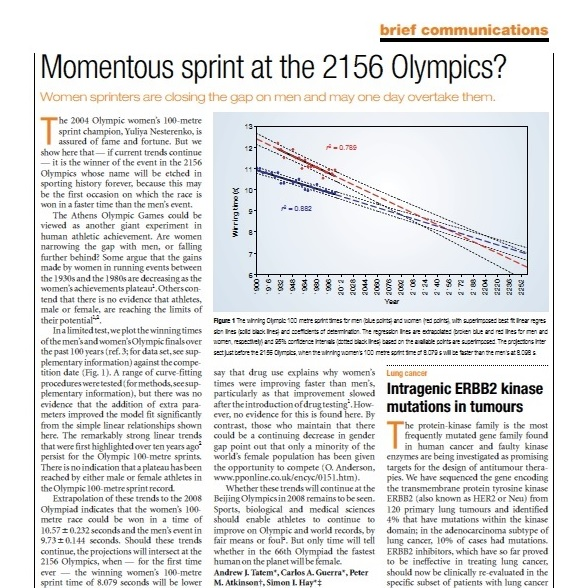
\includegraphics[width=8.12in]{figures/Naturesprint} 

}

\caption{A paper from Nature}\label{fig:Nature2004}
\end{figure}

\textbf{Q1.6} Does this seem reasonable to you? Why?

\textbf{Q1.7} What is the population they are generalising to?

\hypertarget{mmr-innoculation-and-autism}{%
\subsection{MMR innoculation and autism}\label{mmr-innoculation-and-autism}}

If a young child receives the MMR (measles, mumps and rubella) vaccination, are they more likely to become autistic than a child that did not receive the vaccination? In a 1998 paper in the \emph{Lancet}, Andrew Wakefield and co-authors suggested that the MMR vaccination led to intestinal abnormalities, resulting in impaired intestinal function and developmental, 24 hours upto a few weeks of vaccination. This hypothesis was based on 12 children \citep{wakefield1998retracted}. This led to a considerable drop in the percentage of infants and young children being vaccinated.

Some problems identified with this work were:

\begin{itemize}
\item
  too small a sample, not a random nor representative sample (the children had been referred to specialists),
\item
  there was no control group of healthy children for comparison (to see what percentage had autism)
\item
  4 of the 12 children had signs of autism prior to the vaccination
\item
  the authors inferred from this sample that children getting the MMR vaccination were more likely to become autistic than those not getting the vaccine. Thus generalising to all children who have had, or will have, the MMR vaccination.
\end{itemize}

Subsequently, in 2004, 10 of the 13 authors of the study retracted the paper, stating that the data were insufficient to establish a causal link between the MMR vaccine and autism. Arguably the paper lowered vaccination rates in the UK.

\textbf{Q1.8} How safe do you think it was to generalise to all children who have had, or will have, the MMR vaccination?

\hypertarget{two-sid-deaths-in-same-family}{%
\subsection{Two SID deaths in same family}\label{two-sid-deaths-in-same-family}}

How likely is it for two children in the same family to die from Sudden Infant Death (SID), or syndrome (cot death)? Mrs.~Sally Clark was imprisoned in 1999 for the murder of her two infant sons. She was found guilty partially on the basis of Professor Sir Roy Meadow's testimony who said that such an event, two SID deaths in the same family, should only occur with probability one in 73 million. Professor Sir David Cox, a former Professor of Statistics at Imperial College, London, told the General Medical Council's fitness to practise hearing that the odds of two children from the same family dying from sudden infant death syndrome (SIDS) were much higher because they shared the same genetics and were exposed to similar environmental factors. He said Prof.~Meadow's testimony that the chances of Mrs Clark's two babies dying of SIDS were ``one in 73 million should be regarded'' as an error \citep{sallyClarkGuardian}.

The use of statistics in court in the UK has recently been subject to considerable scrutiny see The Inns of Court Council of Advocacy and Royal Statistical Society \citeyearpar{innsof2017court}.

\hypertarget{SUMintro}{%
\section{Summary}\label{SUMintro}}

Numbers and statistics potentially gives us a very powerful way of interpreting and reaching conclusions about the world but they should be used carefully with consideration of bias and uncertainty. This course will help you to critically consider numeric data supplied in news articles and the different types of statistics that are reported.

\hypertarget{ANSintro}{%
\section{Answers}\label{ANSintro}}

\textbf{Q1.1} We should be cautious relying on this claim, see next answer.

\textbf{Q1.2} Consider this as a two stage problem. Can we generalise from 55 mice to all mice (of the species \emph{Mus muscularis})? Perhaps we can, but the laboratory strain of mice might be different to wild mice. Extrapolating to humans may be possible if the physiology of coffee metabolism is similar across species - but it might not be. Dogs, for example, metabolise theobromine, a toxic component of chocolate, at a far slower rate than humans. As a result chocolate is toxic for dogs but is not for humans.

\textbf{Q1.3} Presumably CITES and the Wildlife Conservation Society are using different methods to estimate the sturgeon population. One or both may be wrong.

\textbf{Q1.4} There could be a variety of ways to tackle a problem like this. The fish population could be estimated by seeing how many are captured by fishermen over a given area of ocean. Alternatively perhaps fishes could be marked and released and then recaptured which would allow an estimate of the population size.

\textbf{Q1.5} Requiring fishermen to report their catch accurately might be the cheapest method, otherwise, a dedicated mark recapture approach asin the question above might be necessary.

\textbf{Q1.6} It is a massive extrapolation into the future which assumes a linear trend. There must be a limit to the improvement in sprinter speed. A sprint could not be undertaken in zero seconds!

\textbf{Q1.7} The ``population'' here is not men or women but sprint speeds of men and women.

\textbf{Q1.8} Given it was a biased sample it was probably very unsafe to generalise to all children.

\hypertarget{part-data-collection-and-visualisation}{%
\part{Data Collection and Visualisation}\label{part-data-collection-and-visualisation}}

\hypertarget{sampling}{%
\chapter{Data collection and Sampling}\label{sampling}}

\hypertarget{INTsamp}{%
\section{Introduction}\label{INTsamp}}

Statistics deals with techniques for collecting and analysing data in order to draw conclusions or make some inference. This chapter outlines processes which are used to obtain data in order to draw sound conclusions. The basic techniques incorporate some form of random sampling. This chapter describes the need for sampling, basic sampling strategies, common problems that can afflict the sampling process, and the terminology required.

By the end of the this unit, you should be able to:

\begin{itemize}
\item
  understand the basic principles of sampling
\item
  appreciate the sorts of biases that may occur
\item
  distinguish between accuracy and precision
\item
  understand the difference between experiments and observational studies.
\end{itemize}

\hypertarget{terminology}{%
\subsection{Terminology}\label{terminology}}

We need a common language to talk concisely about statistics and here introduce terms related to sampling that will be used throughout the course:

\begin{itemize}
\item
  \textbf{Sampling unit} \index{Sampling Unit}: an individual object, animal, or person, on which measurements can be made. Essentially this is a discrete entity which is the basis of statistical inference.
\item
  \textbf{Target population}: the overall collection of potential sampling units about which we want to make some inference.
\item
  \textbf{Census}: when the entire target population is sampled/measured.
\item
  \textbf{Sampling protocol or design}: the procedure, or strategy, for selecting sampling units from the target population.
\item
  \textbf{Sample}: a subset of the target population for which measurements on sampling units are made.
\item
  \textbf{Variable}: a characteristic defined for each sampling unit (e.g.~age, weight, blood group) and are typically denoted by lower case Roman letters (e.g.~\(x\), \(y\) represent vectors containing measurements for each sampling unit).
\item
  \textbf{Parameter}: a numerical summary for the target population (e.g.~the mean height of adults in the UK) and are typically denoted by Greek letters (e.g.~\(\mu\), \(\sigma\)) or a numerical characteristic of a statistical model.
\item
  \textbf{Estimate/Statistic}: a numerical summary of a variable for the sample (e.g.~the proportion of a sample of UK citizens that favour a particular political party). Different notation conventions apply to represent estimates from samples, but generally lower case Roman letters are used (e.g.~\(\bar x\) represents the mean of sample data denoted by \(x\)). Note, these statistics are often estimates of a population parameter (e.g.~\(\bar x\) estimates \(\mu\)).
\end{itemize}

\hypertarget{what-is-sampling-and-why-do-it}{%
\section{What is sampling and why do it?}\label{what-is-sampling-and-why-do-it}}

Suppose a landowner has 200 acres of forest where the trees ready for harvest and plans to sell the timber; how could we determine the volume of wood from the forest to get an idea of monetary value? A tree could be a sampling unit and one approach would be to visit every tree, measure its total height, diameter at various heights and calculate the volume. We may also want to ``grade'' the tree in terms of percentage of good wood, lack of defects, decay, etc. In essence, we would be conducting a census of the trees. However, visiting and measuring every tree could be prohibitively expensive, taking far too much time and money.

Therefore, we don't measure all the trees but instead take a sample of plots of land (i.e., a subset of the forest), estimate the volume and grade of trees for each subset. From this the average volume on a plot can be obtained and multiplying this by the total number of plots in the forest will result in an estimate of the total volume of wood in the forest.

In this example, the trees are not necessarily damaged by measuring. In some cases, however, taking a measurement can involve damaging or destroying the unit involved. For example, quality control testing of cans of fizzy drink may involve opening the cans to measure the contents. Taking a census (or indeed sampling a large proportion of the target population) would be clearly counter-productive.

In many cases, it may not be necessary to know the true (i.e.~population) parameter and an estimate will be sufficient. For example, we may not need to know the true volume of wood in the forest and an estimate will be good enough to get an idea of the monetary value of the forest. Therefore, sampling is used rather than take a census. This may be because because we can't measure the entire population: it would be too expensive, take too much time and effort, is impractical or impossible.

\hypertarget{precision-accuracy-and-bias}{%
\subsection{Precision, accuracy and bias}\label{precision-accuracy-and-bias}}

In sampling, we take a sample from a target population and generate a statistic of interest. Suppose we are interested in establishing the proportion of undergraduate students in the University of St Andrews who have a driving licence. We might select a sample of students, ask them whether they have a driving licence and calculate the sample proportion. Image repeating this process with many samples of students. It is likely that the sample proportion will be different for each sample. Ideally, we would like our statistic to be accurate, precise and unbiased (top right in Figure \ref{fig:targetplot}), where

\begin{itemize}
\item
  \textbf{accuracy} implies that each sample statistic is similar to the population parameter
\item
  \textbf{precision} implies that the value of the sample statistic is similar for all samples, and
\item
  \textbf{bias} implies that the sample statistic tends to differ from the population parameter in some consistent way (i.e.~there is a systematic error).
\end{itemize}

In general, a sample statistic will be some combination of the population parameter being estimated plus any bias and some random variability.

\begin{figure}

{\centering 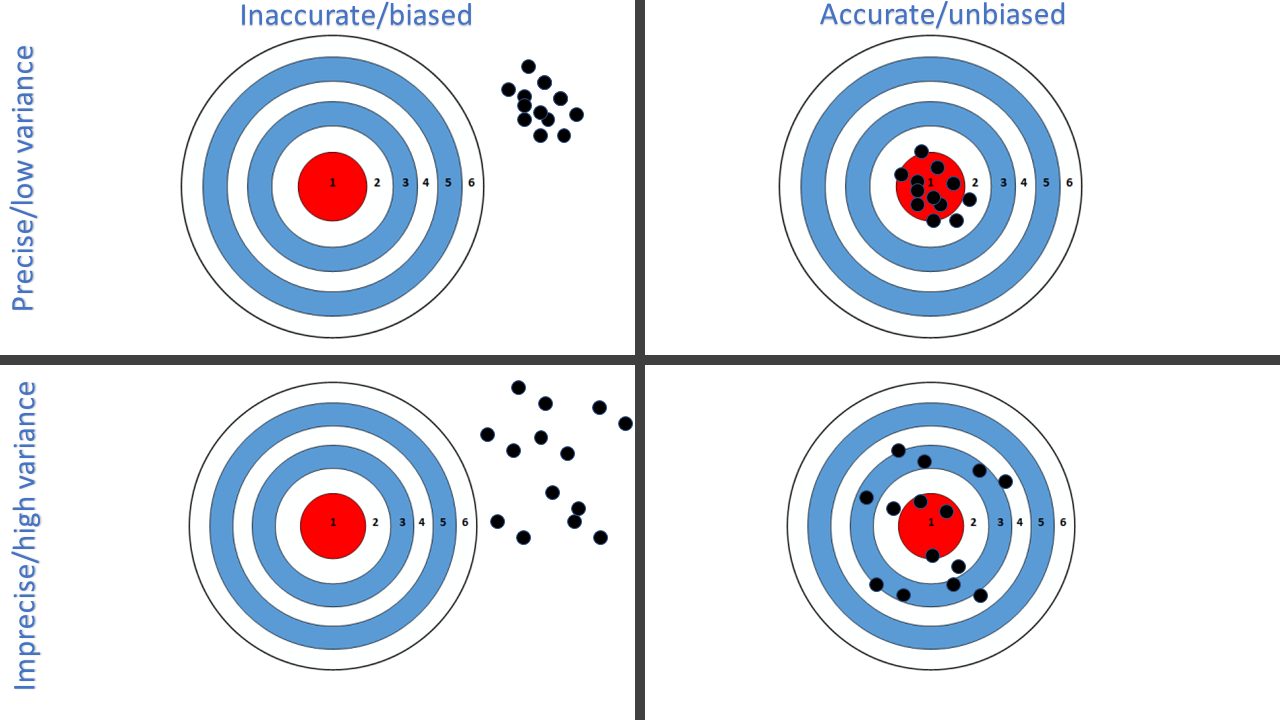
\includegraphics[width=0.95\linewidth]{figures/precision_accuracy_target} 

}

\caption{The centre of the target indicates the true value of the parameter and the dots are sample statistics.}\label{fig:targetplot}
\end{figure}

\textbf{Q2.1} A headline on the BBC website stated that ``Vapers rise `to more than three million' in Britain'' (\href{https://www.bbc.co.uk/news/health-45513762}{BBC, 14/09/2018}). The article goes onto state that the numbers of e-cigarette users has risen from from 2.9m to 3.2m between 2017 and 2018 - a rise of 10\%. It is likely that a sampling survey has been undertaken to obtain these numbers.

\textbf{a.} What is the target population?

\textbf{b.} What is the sampling unit?

\textbf{c.} What is the variable being measured?

\textbf{d.} What is the population parameter?

\textbf{e.} What is the sample estimate?

\hypertarget{three-types-of-data-collection}{%
\section{Three types of data collection}\label{three-types-of-data-collection}}

There are three general procedures for collecting data and each are covered in this chapter:

\begin{itemize}
\item
  sample surveys (and polls)
\item
  designed experiments
\item
  observational studies.
\end{itemize}

Statisticians make a distinction between experiments and observation studies (also known as quasi-experiments \footnote{This is one definition of quasi-experiment, there are others}).

It is important to emphasise that how data are collected affects the ability to learn about the world. Flawed data collection procedures can make it impossible, or nearly so, to arrive at quality decisions or to make accurate statements. In many cases, no amount of sophisticated data analysis procedures will remedy ``bad data''. Notably, whatever method is used for the collection/generation of data, sampling is likely to underpin the collection process. From the outset there is inherent uncertainty surrounding our ability to produce answers for a population from a sample, hence, robust sampling strategies need to be used when selecting a sample.

\hypertarget{common-but-unwise-data-collection-strategies}{%
\subsection{Common, but unwise, data collection strategies}\label{common-but-unwise-data-collection-strategies}}

For sample estimates to be applicable to the target population from which the sample was taken, the sample needs to be representative. Two approaches to sampling which generally lead to unrepresentative (i.e.~biased) samples are anecdotal evidence and self-selected samples.

\begin{itemize}
\item
  Anecdotal evidence can be based on haphazardly selected individual cases, which often come to our attention because they are striking in some way. These cases need not be representative of any larger group of cases.
\item
  Self-selected, or voluntary response, samples are commonplace; magazines and newspapers often include questionnaires that readers can complete and send back. Internet polls are much the same, as are opt-in surveys: individuals choose whether or not they want to respond and hence be included in the sample.
\end{itemize}

Principally, we want any sample statistic to have:

\begin{itemize}
\item
  high precision/low uncertainty,
\item
  high accuracy, and hence low bias,
\end{itemize}

as per top right panel in Figure \ref{fig:targetplot}. There can be many sources of inaccuracy and/or a lack of precision, but fortunately some of them can be controlled. Sampling is a just such a controllable source and three frequently used strategies are described below.

\textbf{Q2.2} Considering phone-in programmes on the radio, are the opinions expressed representative of the UK population, or even of all the people who listen to the radio show? What type of person is likely to call?

\hypertarget{simple-sampling-approaches}{%
\section{Simple sampling approaches}\label{simple-sampling-approaches}}

Having decided to take a sample from our target population, the next question is how to choose the sample. All good sample schemes have two features:

\begin{itemize}
\item
  planned randomness, and
\item
  the chance, or probability, that any given sampling unit being selected can be calculated.
\end{itemize}

These features ensure that sample is representative of the population; i.e., one has controlled for \textbf{selection bias}, the bias that results when part of the target population is systematically excluded from the samples.

Sampling is a large topic of study in itself; here we consider three basic strategies:

\begin{itemize}
\item
  Simple random samples
\item
  Systematic random samples
\item
  Stratified random samples
\end{itemize}

\hypertarget{simple-random-sample}{%
\subsection{Simple random sample}\label{simple-random-sample}}

A simple random sample (SRS) is a subset of the target population in which each sampling unit has an equal chance of being selected. The chance, or probability, of a sampling unit being selected can be calculated easily. Say the target population is of size \(N\) and the sample size is \(n\), then the probability of an individual sampling unit being selected is \(n/N\).

\textbf{Example} We want to select 10 students from a group of 150 using simple random sampling. The probability of an individual student being selected is \(\frac{10}{150}\).

How do we ensure that each sampling unit has an equal chance of being selected? One way would be to assign a number to each individual, write each number on a slip of paper, put the slip of papers in a hat, mix thoroughly and draw 10 slips out - the numbers on the slips of paper determine who is selected. Alternatively, a computer could be used to generate 10 numbers from a list of numbers 1 to 150.

\hypertarget{doing-this-in-r}{%
\subsubsection{Doing this in R}\label{doing-this-in-r}}

\begin{Shaded}
\begin{Highlighting}[]
\CommentTok{\# Generate a simple random sample of size 10 from a population of 150 units}

\CommentTok{\# Initialise necessary objects}
\NormalTok{N }\OtherTok{\textless{}{-}} \DecValTok{150} \CommentTok{\# Size of target population}
\NormalTok{n }\OtherTok{\textless{}{-}} \DecValTok{10} \CommentTok{\# Sample size}
\CommentTok{\# SRS }
\FunctionTok{sample}\NormalTok{(}\AttributeTok{x=}\DecValTok{1}\SpecialCharTok{:}\NormalTok{N, }\AttributeTok{size=}\NormalTok{n, }\AttributeTok{replace=}\ConstantTok{FALSE}\NormalTok{)}
\end{Highlighting}
\end{Shaded}

\begin{verbatim}
 [1]  54 148  72 131  53   7 150  17 123  96
\end{verbatim}

\begin{Shaded}
\begin{Highlighting}[]
\CommentTok{\# The sample doesn\textquotesingle{}t have to be numbers}
\NormalTok{IDs }\OtherTok{\textless{}{-}} \FunctionTok{c}\NormalTok{(}\StringTok{"subject1"}\NormalTok{, }\StringTok{"subject2"}\NormalTok{, }\StringTok{"subject3"}\NormalTok{, }\StringTok{"subject4"}\NormalTok{, }\StringTok{"subject5"}\NormalTok{)}
\FunctionTok{sample}\NormalTok{(}\AttributeTok{x=}\NormalTok{IDs, }\AttributeTok{size=}\DecValTok{2}\NormalTok{, }\AttributeTok{replace=}\ConstantTok{FALSE}\NormalTok{)}
\end{Highlighting}
\end{Shaded}

\begin{verbatim}
[1] "subject5" "subject1"
\end{verbatim}

It is worth spending a minute thinking about computer-generated random numbers. Computers are not random, however, they can be `effectively' random with pseudo-Random Number Generators (RNGs). There are many types of RNGs, but all are effectively unpredictable without knowing a starting point. In the examples below, we generate a sample of numbers with and without specifying the starting point.

First, we don't specify the starting point and so each time we generate a sample of numbers, the samples are different.

\begin{Shaded}
\begin{Highlighting}[]
\CommentTok{\# Example when the result is unpredictable}

\CommentTok{\# Generate 4 decimal numbers from 0 to 1 (a uniform (0,1) distribution) }
\FunctionTok{runif}\NormalTok{(}\AttributeTok{n=}\DecValTok{4}\NormalTok{, }\AttributeTok{min=}\DecValTok{0}\NormalTok{, }\AttributeTok{max=}\DecValTok{1}\NormalTok{)}
\end{Highlighting}
\end{Shaded}

\begin{verbatim}
[1] 0.4423083 0.7968483 0.3036517 0.5053533
\end{verbatim}

\begin{Shaded}
\begin{Highlighting}[]
\CommentTok{\# Repeat}
\FunctionTok{runif}\NormalTok{(}\AttributeTok{n=}\DecValTok{4}\NormalTok{, }\AttributeTok{min=}\DecValTok{0}\NormalTok{, }\AttributeTok{max=}\DecValTok{1}\NormalTok{)}
\end{Highlighting}
\end{Shaded}

\begin{verbatim}
[1] 0.2864899 0.4160687 0.6282003 0.6029328
\end{verbatim}

But - with a seed, a starting point for the RNG, the generated numbers are predictable/reproducible.

\begin{Shaded}
\begin{Highlighting}[]
\CommentTok{\# Set the seed for the RNG}
\FunctionTok{set.seed}\NormalTok{(}\DecValTok{2343}\NormalTok{)}
\FunctionTok{runif}\NormalTok{(}\AttributeTok{n=}\DecValTok{4}\NormalTok{, }\AttributeTok{min=}\DecValTok{0}\NormalTok{, }\AttributeTok{max=}\DecValTok{1}\NormalTok{)}
\end{Highlighting}
\end{Shaded}

\begin{verbatim}
[1] 0.20467634 0.09047926 0.61101041 0.17877428
\end{verbatim}

\begin{Shaded}
\begin{Highlighting}[]
\CommentTok{\# Repeat}
\FunctionTok{set.seed}\NormalTok{(}\DecValTok{2343}\NormalTok{)}
\FunctionTok{runif}\NormalTok{(}\AttributeTok{n=}\DecValTok{4}\NormalTok{, }\AttributeTok{min=}\DecValTok{0}\NormalTok{, }\AttributeTok{max=}\DecValTok{1}\NormalTok{)}
\end{Highlighting}
\end{Shaded}

\begin{verbatim}
[1] 0.20467634 0.09047926 0.61101041 0.17877428
\end{verbatim}

Setting the seed is useful for confirming calculations which have a stochastic, or random, component.

\hypertarget{systematic-samples}{%
\subsection{Systematic samples}\label{systematic-samples}}

Suppose there are \(N=1000\) individuals in the target population and we want to take a sample of size \(n=200\). A systematic sample can be selected as follows:

\begin{enumerate}
\def\labelenumi{\arabic{enumi}.}
\item
  Calculate the fixed periodic interval, \(k = N/n\). In our example, this is \(k = 1000/200 = 5\).
\item
  Randomly pick a starting number between 1 and \(k\), call it \(q\), say \(q=3\)
\item
  Sample the \(q\)th individual, then the (\(q+k\))th, then (\(q+2k\))th and so on. Thus, starting at \(q=3\), the sample will be generated by 3, (3+5), (3+2x5), and so on; the sample will consist of sampling units 3, 8, 13, \ldots, 993, 998.
\end{enumerate}

Systematic samples have some advantages over SRS:

\begin{itemize}
\item
  it is often easier to draw since only one number is randomly selected (i.e.~\(q\)).
\item
  it will distribute the sample more evenly through the population.
\item
  it will do better than a SRS if there is a trend in the values.
\end{itemize}

\textbf{Example} We want to take a sample of customers visiting a bank. From a practical point of view, it is much easier to pick every 10th person, say, arriving in the bank than refer to a SRS of bank customers. In addition, SRS could, by chance, select a lot of customers in the morning which could be a particular subset of the customers if there is a pattern in the type of customers that arrive through the day. A systematic sample would spread the selected customers throughout the day.

One thing to be aware of is, if the population contains some variation which is periodic in nature and if the fixed periodic interval (\(k\)) equals the periodic variation, the sample may be biased. Consider loaves of bread on a production line; each loaf is cut into 20 slices. A slice is taken from each loaf. Using a systematic sample with a fixed interval of \(k=20\), the sample will consist of either all crusts or no crusts, depending on the starting value.

\hypertarget{doing-this-in-r-1}{%
\subsubsection{Doing this in R}\label{doing-this-in-r-1}}

The code below selects a systematic sample.

\begin{Shaded}
\begin{Highlighting}[]
\CommentTok{\# Draw a systematic random sample of size 20 from a population of 100 units}

\CommentTok{\# Initialise values}
\NormalTok{N }\OtherTok{\textless{}{-}} \DecValTok{100} \CommentTok{\# Size of target population}
\NormalTok{n }\OtherTok{\textless{}{-}} \DecValTok{20} \CommentTok{\# Sample size }
\CommentTok{\# Calculate fixed periodic interval k}
\NormalTok{k }\OtherTok{\textless{}{-}}\NormalTok{ N}\SpecialCharTok{/}\NormalTok{n}
\NormalTok{k}
\end{Highlighting}
\end{Shaded}

\begin{verbatim}
[1] 5
\end{verbatim}

\begin{Shaded}
\begin{Highlighting}[]
\CommentTok{\# Randomly select starting point q}
\NormalTok{q }\OtherTok{\textless{}{-}} \FunctionTok{sample}\NormalTok{(}\DecValTok{1}\SpecialCharTok{:}\NormalTok{k, }\AttributeTok{size=}\DecValTok{1}\NormalTok{)}
\NormalTok{q}
\end{Highlighting}
\end{Shaded}

\begin{verbatim}
[1] 3
\end{verbatim}

\begin{Shaded}
\begin{Highlighting}[]
\CommentTok{\# Generate regular sequence}
\FunctionTok{seq}\NormalTok{(}\AttributeTok{from=}\NormalTok{q, }\AttributeTok{to=}\NormalTok{N, }\AttributeTok{by=}\NormalTok{k)}
\end{Highlighting}
\end{Shaded}

\begin{verbatim}
 [1]  3  8 13 18 23 28 33 38 43 48 53 58 63 68 73 78 83 88 93 98
\end{verbatim}

\hypertarget{stratified-random-samples}{%
\subsection{Stratified random samples}\label{stratified-random-samples}}

In a stratified random sample, the population is divided into different groups or ``strata'', then simple random samples are selected from each stratum. For example, we might divide the population of the university into four strata (e.g.~undergraduate students, postgraduate students, academic and research staff, and support staff) and take a SRS from each strata. Why do this?

\begin{itemize}
\item
  Sometimes it is more convenient to organise sampling in this way and choose a SRS within a homogeneous group.
\item
  The stratification ensures that all strata will be represented in the overall sample, which may not be the case for a SRS.
\item
  It may be useful to examine the separate statistics from each strata.
\item
  It can result in greater precision when estimating a parameter than for a SRS with the same sample size because sampling units within a stratum may be more similar (hence reducing variability).
\item
  The size of the sample in each stratum can be proportional to the total number of sampling units in each stratum so that each stratum is represented equally.
\end{itemize}

The proportion of sampling units in stratum \(i\), \(p_i\), can be found from

\[p_i = \frac{N_i}{N} \]
where \(N_i\) is the total number of sampling units in stratum \(i\). For a total sample of size \(n\), then the number selected from group \(i\) can be calculated from
\[n_i = n \times p_i\]

This strategy is frequently used in environmental studies, for example, in fisheries stock assessment where different areas (strata) are sampled with different intensity.

\textbf{Q2.3} In 2019, the population of the University of St Andrews was made up of members classed in one of four groups (size of the group is given in parentheses):

\begin{itemize}
\item
  undergraduate students (7,221),
\item
  postgraduate students (1,763),
\item
  academic and research staff (1,426), and
\item
  support staff (1,174).
\end{itemize}

\textbf{a.} For a simple random sample of size 500, what is the probability of an individual member of the University being selected?

\textbf{b.} If we take a systematic sample of size 500, what is the fixed period interval, \(k\)?

\textbf{c.} Assume that all members of staff are assigned a number. Given a starting number of \(q = 12\), what are the first five numbers of a systematic sample that would be selected using the value of \(k\) calculated in part 2a?

\textbf{d.} We now want to take a stratified random sample, using the groups as the strata, and sample in proportion to the strata sizes. What will be the sample size for each group if the total sample size is 500?

\hypertarget{sampling-biases}{%
\section{Sampling biases}\label{sampling-biases}}

Sampling error is incurred when the characteristics of interest in a population are estimated from a sample - it is the difference between the sample statistics and the true, but unknown, parameter of the population - and is unavoidable. There will also be random variation between samples - sampling error is also used more broadly to refer to this sample-to-sample variation. Therefore, it is important that our samples are representative of the population as a whole. In essence, we want any differences between our samples and the population to be due to random variation only and not due to other sources of error.

Selecting a sample in such a way that it is unrepresentative of the target population has been mentioned and will cause bias, however, even if a random sample is selected in some way, then serious biases can still occur.

\hypertarget{non-sampling-error}{%
\subsection{Non-sampling error}\label{non-sampling-error}}

Even though a random sample has been selected, sources of error, or bias, can occur when collecting data. A few common sources of error when surveying people in particular are listed below.

\textbf{Non-response bias}

When surveying people, a certain percentage of the sample will not provide information even though they have been selected to take part. The reasons for non-response will be many and may include not being at home, too busy, or having a dislike for pollsters. If the values of the variable(s) being measured differs between non-responders and responders, then the resulting statistic can be severely biased.

\textbf{Survey format}

The format of a survey (e.g.~postal questionnaire, by telephone, in person) may affect the results. For example, respondents may not feel comfortable giving personal information to an interviewer (e.g.~``How old are you?'') but more willing to provide the information in a postal questionnaire.

\textbf{Question effects}

Questions can be slanted in a particular way, or lead the respondent on purpose; for a well-designed survey this should be guarded against. The choice of words is also important as the following example illustrates.

\emph{Example} (from \citep{moore2003}) When asked `How do the Scots feel about the movement to become independent from England?' 51\% of the sample voted for ``independence for Scotland'', but only 34\% supported ``an independent Scotland separate from the United Kingdom''. It seems that the wording of the question had an effect; maybe ``independence'' is a nice, hopeful word while ``separate'' is a negative word.

Poor quality data can also arise depending upon length of survey; the respondent may get tired or bored if there are too many questions, or question response categories, to consider. The questions should also be in some logical order and not jump between topics which may confuse the respondent.

\textbf{Response bias}

The behaviour of the respondent or of the interviewer can influence responses in several ways.

An interviewer can intimidate or alienate the respondent, albeit unintentionally (e.g., different race or social class) leading the respondent to answer untruthfully.

A respondent may not answer truthfully because a question may have:

\begin{itemize}
\item
  a social stigma (or legal implications) related to it (e.g.~``Have you ever been arrested?'')
\item
  a social prestige slant (e.g.~``How much money do you earn?'').
\end{itemize}

Respondents may

\begin{itemize}
\item
  answer in a way that is socially acceptable (e.g.~to the question ``How many units of alcohol do you drink per week?'')
\item
  suffer from recall bias so that they cannot remember exactly when something happened or what happened (e.g.~``How many hours of television did you watch last Thursday?'')
\item
  misunderstand the question (e.g.~giving weight in kilograms instead of pounds).
\end{itemize}

Careful and thoughtful questionnaire design is important\textbackslash footnote\{Further reading can be found \href{https://www.pewresearch.org/methods/u-s-survey-research/questionnaire-design/}{here}. Any questionnaire should be tested to eliminate any inconsistencies or confusion before it is used for real.

\textbf{Q2.4} In 1936, a magazine in the USA called the \textit{Literary Digest} sent out 10 million questionnaires to people drawn from car registration lists and telephone directories asking who they would vote for in the upcoming election; 2.3 million questionnaires were returned. From the results, the magazine predicted a landslide victory for Republican candidate Alf Landon. In fact, the Democrat candidate, Franklin Roosevelt, won the election. With such a large number of questionnaires returned, what do you think went wrong?

\textbf{Q2.5} A psychologist was interested in understanding the motivation of serial killers and in estimating the mean number of victims per serial killer. The psychologist discovered there were 261 serial killers incarcerated worldwide.

\textbf{a.} The psychologist initially planned to interview all imprisoned serial killer about various aspects of their personality. Describe the approach being used.

\textbf{b.} This initial approach proved to be too costly, therefore, the psychologist randomly choose 80 killers to contact and ask if they were prepared to be interviewed. Thirty-nine agreed to be interviewed. Comment on the representativeness of the sample to the whole population of worldwide serial killers and what type of bias this may result in, if any.

\textbf{c.} In choosing the initial 80 prisoners, the psychologist selected them randomly in proportion to the overall number of imprisoned serial killers in each country e.g.~if 50\% of the world's convicted serial killers were in prisons in the USA, then 40 serial killers in the USA were selected at random. What sort of sampling design is this?

\hypertarget{experiments}{%
\section{Experiments}\label{experiments}}

The \citep{dictionary1980oxford} gives the following definition (one of several) for an experiment: \emph{An action or operation undertaken in order to discover something unknown, to test a hypothesis, or establish or illustrate some known truth.}

In an experiment, we often try to discover whether a ``treatment'' or ``condition'' has an effect on sampling units, or experimental units, and what the nature and magnitude of that effect is. Typically there is a \textbf{manipulation} or \textbf{intervention}. Note that if the experimental units are animals, they are known as ``subjects'' and if the experimental units are humans they are increasingly referred to as ``participants''. Experiments do not have to be done in the laboratory, they can be undertaken anywhere, for example, experiments might be used to answer the following questions:

\begin{enumerate}
\def\labelenumi{\arabic{enumi}.}
\tightlist
\item
  Does a certain drug improve the prospects for heart transplant patients?
\item
  Does heating a wire increase its electrical resistance?
\item
  How effective is an insecticide?
\end{enumerate}

To investigate these questions, we give different treatments to different experimental (sampling) units and measure a \textbf{response}. In the examples, above, these might be:

\begin{longtable}[]{@{}lll@{}}
\toprule
Example & Experimental unit & Treatment\tabularnewline
\midrule
\endhead
1 & patient & drug\tabularnewline
2 & wire & heat\tabularnewline
3 & mosquito & insecticide\tabularnewline
\bottomrule
\end{longtable}

There is often some natural variability in the results of any experiment. Using statistics, we aim to disentangle this natural variation from any variation that is introduced by our treatment method.

\hypertarget{randomised-experiments}{%
\subsection{Randomised experiments}\label{randomised-experiments}}

In a randomised experiment, treatments are randomly allocated to experimental units by the researcher.

\textbf{Example} A new drug for heart-transplant patients is to be tested against a standard drug. Patients in the study are randomly allocated to either the new or standard drug group. Each patient in the heart-transplant study has an equal chance of being selected for the group that will be given the new drug.

A difference in the response between the two groups can be attributed to the treatment because the patients were randomly allocated to treatments.

\textbf{Example} A new insecticide is developed for the control of mosquitoes for use in countries where malaria is a significant problem. How effective is it, and will it be cheaper or more expensive to use than existing chemical treatments?

The insecticide is designed for use with adult mosquitoes and a scientist might set up an experiment like this:

\begin{itemize}
\item
  Create 4 separate enclosures
\item
  Place a sample of the same number of adult mosquitoes in each enclosure.

  \begin{itemize}
  \tightlist
  \item
    These individuals are the experimental units in this experiment.
  \end{itemize}
\item
  Choose 4 different concentrations of insecticide, one for each enclosure.

  \begin{itemize}
  \tightlist
  \item
    Apply the treatment each day by spraying enclosure with insecticide.
  \item
    The concentration of insecticide is a factor known as the explanatory variable.
  \end{itemize}
\item
  One treatment should be a control in which no insecticide is applied, but a water spray is applied (in case mosquitoes are actually killed when sprayed).
\item
  Determine how many mosquitoes in each enclosure survive, and how many die (mortality, in this case, is the response variable/variable of interest).
\item
  Repeat (replicate the whole experiment) 10 times.

  \begin{itemize}
  \tightlist
  \item
    We can then see how much natural variation occurs in the results of the experiment
  \item
    this enables us to determine whether the treatment has a real effect on the outcome or if any differences are down to natural variability alone.
  \end{itemize}
\item
  Randomly assign experimental units (mosquitoes) to the 4 treatments and 10 replicates. This should get around possible biases

  \begin{itemize}
  \tightlist
  \item
    e.g.~if ``fitter'' individuals are selected for one treatment.
  \item
    Differences in responses should then only be due to the effect of the treatments.
  \end{itemize}
\end{itemize}

\hypertarget{components-of-an-experimental-design}{%
\subsection{Components of an experimental design}\label{components-of-an-experimental-design}}

\textbf{Randomization} may be carried out by assigning numbers to individuals, then picking numbers at random. Randomization is done to ensure that treatment groups are, on average, similar.

\begin{itemize}
\tightlist
\item
  Randomization is designed to avoid bias.
\end{itemize}

\textbf{Replication} is carried out in order to:

\begin{itemize}
\item
  assess the amount of natural variation in the results. This way, it is possible to determine whether a treatment has a significant effect.
\item
  increase precision. The more replicates, the more precise the result (but the greater the cost in time and money!)
\end{itemize}

As a rule of thumb, the number of replicates should be at least twice the number of treatments with an absolute minimum of 6 per treatment.

Sometimes, the experimental units (or subjects) are partitioned into stratum, or \textbf{blocked}. For example,
in the mosquito experiment, individuals could be assigned to ``male'' and ``female'' groups (strata) before being randomly allocated to a particular treatment. This may reduce the amount of natural variability in the results of an experiment, so that the results are more precise.

In studies involving human subjects, for example in drug trials, a \textbf{placebo} may be given to a control group.

\begin{itemize}
\item
  A placebo is a `treatment' (e.g.~drug or intervention) with no known active effects e.g.~sugar pills.
\item
  It is given so that the patient does not know what treatment they are receiving because there may be a psychological effect when a doctor offers a patient a treatment.
\end{itemize}

It may also be necessary to use \textbf{double blinding} so that the doctor does not know what treatment they are offering and the patient does not know what treatment they are receiving. This avoids subtle differences in the behaviour of doctors according to the treatment they are prescribing.

If a randomised experiment shows a significant effect, it is possible to argue for causation i.e.~that the treatment caused the effect.

\textbf{Example} A famous and large-scale designed experiment that is still relevant today is Salk's polio vaccine study.

Polio (poliomyelitis) is a serious viral infection that used to be common worldwide. It caused muscle weakness from which a small percentage of people did not recover and even died. The number of cases in the US during the mid 20th century are shown in Figure \ref{fig:polio}.

\begin{figure}[!htbp]

{\centering 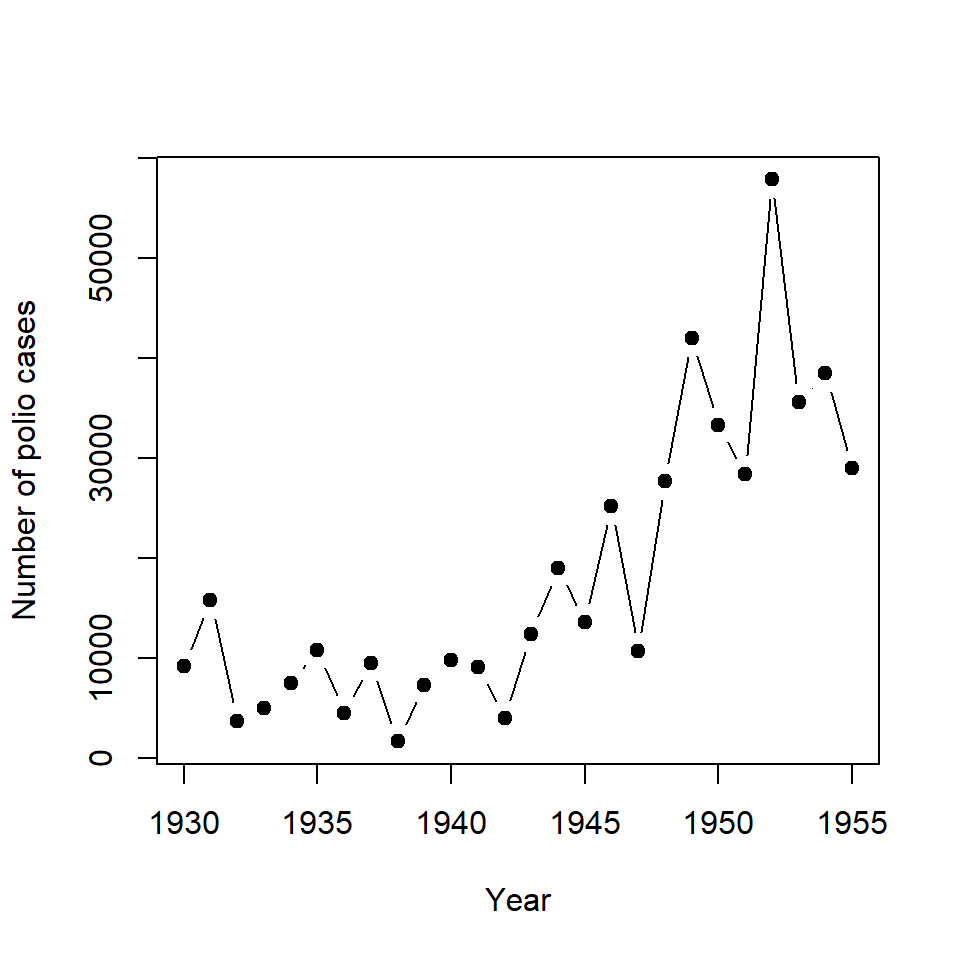
\includegraphics{IntroStats_files/figure-latex/polio-1} 

}

\caption{The number of polio cases from 1930 to 1955}\label{fig:polio}
\end{figure}

\begin{itemize}
\tightlist
\item
  In general, the incidence of polio was increasing over this time period.
\item
  However, the incidence of disease also fluctuates from year to year, with high and low incident years sometimes alternating.
\end{itemize}

Jonas Salk's created a vaccine and a large-scale trial of this vaccine was conducted in the US in 1954 to determine how effective it was in protecting children from paralysis or death due to polio. Snedecor and Cochran (\citeyearpar{Snedecor&Cochran1980}) describe the study in detail; a summary is provided here. School children were divided into two groups; one group received the vaccine (the treatment group) and the other group received no vaccine (control group). The comparison of the numbers of paralytic cases in each group were used to judge the effectiveness of the vaccine. Since severe symptoms are rare, large numbers of children were required and more than 200,000 children were recruited to each group. Within each participating school, children were randomised such that there were about equal numbers of children in each group. This stratified approach ensured that schools in high risk and low risk regions had about equal numbers of children in each group. A simple randomisation of children to the groups would mean that overall the numbers in the two groups were equal but would not take account of high and low risk regions.

The children in the vaccine group received three injections of the vaccine and the children in the comparison, or control, group received three injections of a saline solution. They were given at the same time and in the same manner.
A crucial aspect of the study was that neither parents, children, medics administering the vaccine or the doctors diagnosing illness knew which treatment group the children were in - this was a \textbf{double-blind trial}.

The following table shows the numbers of children in each of the groups and the number of polio cases (\citep{Snedecor&Cochran1980}, pg. 13):

\begin{longtable}[]{@{}lll@{}}
\toprule
~ Group & Number of children & Polio cases per 100,000\tabularnewline
\midrule
\endhead
Vaccinated & 200,745 & 16\tabularnewline
Control & 201,229 & 57\tabularnewline
\bottomrule
\end{longtable}

The trials provided good evidence for the effectiveness of the vaccine. Regular use of polio vaccine since the Salk trial has reduced the incidence of the disease dramatically.

\begin{center}\rule{0.5\linewidth}{0.5pt}\end{center}

To summarise, in an experiment we often try to determine whether a `treatment' (or intervention of some kind) has a significant effect.

\begin{itemize}
\item
  A \textbf{control group} is a group of units that are not exposed to the treatment. This group is generally necessary for comparison with the treatment group to assess the effectiveness of the treatment.
\item
  In a \textbf{randomised experiment}, subjects/experimental units are assigned to the treatment or control group at random.
\item
  In \textbf{blocked experiments}, the experimental units may first be divided into strata or groups (e.g.~on the basis of age).
\item
  Experiments should be replicated.
\item
  In drug trials, patients in the control group may be given a \textbf{placebo} (an inactive pill or medicine) so that they do not know whether they are in the control or treatment group
\item
  If the doctor also does not know which group the patient is in, this is a \textbf{double-blind} trial
\item
  If a randomised experiment produces a significant effect, then we can argue for a \textbf{causal link} between treatment and effect.
\end{itemize}

\hypertarget{controls}{%
\subsection{Controls}\label{controls}}

Controls are benchmarks required for a comparison, they are frequently used \textbf{but not necessarily essential}. For example, one might be interested in knowing whether having a cup of coffee elevates heart rate. Here a control is essential, otherwise how would one know if an elevation in heart rate was due to the coffee or because the heartbeat was being measured.

Sometimes a control is not necessary, for example if the question was ``Do different sorts of coffee have different effects on heart rate?'' The natural experiment would be to compare different varieties of coffee, no control is required because, here, we have \textbf{a contrast}.

\textbf{Q2.6} A doctor is investigating the potential effect of a new drug in combating an as yet incurable disease. Is a control required?

\textbf{Q2.7} A pharmaceutical company is testing whether a new experimental drug is better than the existing treatments on the market. Is a control required?

\hypertarget{observational-studies}{%
\section{Observational Studies}\label{observational-studies}}

Observational studies refer to data collected from `nature' without any kind of manipulation and so conditions are NOT under the control of the researcher. This terminology is commonly used across most of science, however alternative terminology is sometimes used; astronomers often refer to theory-based observation of stars, galaxies, gas clouds as ``experiments'' although in no sense are they manipulating the cosmos!

\textbf{Example} Let us return to the mosquito example. Imagine that villagers have already been using the new insecticide in the field. They have used the chemical at various concentrations. A scientist surveys the area and determines the population density of mosquitoes in different locations.
This scientist also collects information from the local people as to what concentration of insecticide they have been using.

This looks quite similar to the previous study. However, the results are more difficult to interpret because:

\begin{itemize}
\item
  we do not know if there are naturally-occurring differences in mosquito population density in the different areas due to ``other factors''. For example, there may be other animals that eat mosquitoes in one area and so the density is reduced (a \textbf{confounding variable}).
\item
  we do not know that the mosquitoes themselves are ``all the same'', e.g mosquitoes in one area may be genetically different to those in another area (another confounding variable).
\end{itemize}

It is more difficult to argue for \textbf{causation} based on an observational study because of potential confounding variables. It is important to remember this when reporting on the outcome of a statistical investigation. However, in practice, observational studies often have to be used as evidence for an effect because:

\begin{itemize}
\item
  It may be difficult, in practice, to carry out a randomized experiment, e.g.~the effects of fishing on a large ecosystem such as the North Sea cannot be explored by conducting experiments on a series of ``replicate'' oceans.
\item
  It may be unethical to carry out a randomized experiment:

  \begin{itemize}
  \tightlist
  \item
    e.g imagine that we want to know about the implications of smoking for human health. We are interested in knowing what effect of mothers smoking during pregnancy has on the average birth-weight of babies. It would not be ethical to ask a randomly-chosen group of mothers to take up smoking, because this might adversely affect their unborn babies or their own health.
  \end{itemize}
\end{itemize}

Therefore, we have to examine other kinds of evidence:

\begin{itemize}
\tightlist
\item
  randomised experiments carried out on animals
\item
  observational studies, e.g.~looking at birth weights of babies born to mothers who have chosen not to smoke and weights of babies born to mothers who have chosen not to give up smoking in pregnancy.
\end{itemize}

Remember that an observational study is not a randomized experiment, we may not be able to make a strong argument for causation based on the results. For example, if it is found that babies where the mothers smoked during pregnancy have generally lower birth weight, this could be due to confounding variables, such as diet.

\hypertarget{types-of-observational-study}{%
\subsection{Types of observational study}\label{types-of-observational-study}}

There are a variety of types of observational study. Some of which are given specific definitions:

\begin{itemize}
\item
  \textbf{Cohort study}: A cohort is any group of people who are linked in some way. For instance, a birth cohort includes all people born within a given time frame. Researchers compare what happens to members of the cohort that have been exposed to a particular variable to what happens to the other members who have not been exposed.
\item
  \textbf{Case control study}: Researchers identify people with an existing health problem (`cases') and a similar group without the problem (`controls') and then compare the two groups with respect to an exposure or exposures.
\end{itemize}

These studies can be \textbf{prospective} or \textbf{retrospective}:

\begin{itemize}
\item
  Prospective: none of the subjects have the disease (or other outcome of interest) when the study commences; the subjects are followed over a period of time to determine whether the disease develops.
\item
  Retrospective: the researcher looks at historical data to examine previous exposure to suspected factors in relation to an outcome determined at the start of the study.
\end{itemize}

\textbf{Example} UK Millennium cohort study

Known as the `Child of the New Century' project, the lives of nearly 19,000 children born in the UK during 2000 and 2001 were followed. Data were collected when they were 9 months, 3, 5, 7, 11, 14 and 17 years. A large number of studies have been conducted of the data collected looking at, for example, health, behavioural problems, career aspirations. Details can be found \href{https://cls.ucl.ac.uk/cls-studies/millennium-cohort-study/}{here}

\textbf{Example} A retrospective, case control observational study on smokers

To determine the death rate of men with different smoking habits, large studies were undertaken between 1951 and 1959 (\citeyearpar{Snedecor&Cochran1980}). A questionnaire was sent to the selected group of men asking about current and past smoking habits and other information, such as age. The study compared different groups whose death rates could be compared (e.g.~different types of smokers - nonsmokers, cigarettes, cigars, pipes, mixed).

If death rates were found to be different between the groups it would still be difficult to conclude this was due to the smoking habits. The subjects assigned themselves to groups by their smoking habits and the groups may differ in other ways apart from their smoking habits (e.g.~age, income, lifestyle).

To control for other factors, the researchers must try to control for these other factors and divide the subjects into groups such that these other factors are similar. Then, for example, compare the death-rates of smokers and non-smokers who are in the same age category.

\textbf{Example} A retrospective, case control study on sudden infant death syndrome (SIDS)

A large study on SIDS cases in Scotland were investigated from 1992 to 1995. When a case of SIDS occurred, the parents were interviewed to find out about methods of infant care and socioeconomic factors. Two controls were chosen for each case by identifying babies born in the same maternity unit and just before/after the SIDS baby, thus controlling for time of year and age and maternity unit. More details \href{http://www.sids-network.org/experts/scottish.htm}{here}

\begin{center}\rule{0.5\linewidth}{0.5pt}\end{center}

To summarise, there are two main types of observational study, \textbf{cohort} and \textbf{case control} studies.

\begin{itemize}
\item
  A \textbf{prospective study} is one in which samples are chosen, and variables measured, and the subjects (or units) are subsequently observed over time in order to observe the outcomes. The relationship between the initial measured variable on the outcome can be studied.
\item
  In a \textbf{retrospective case-control study}, cases in which a certain outcome has occurred are compared with controls in which that outcome has not occurred. Differences between the case and control groups may indicate factors that are correlated with certain outcomes.
\item
  A \textbf{confounding variable} is some factor not accounted for, which introduces a difference in outcomes between treatment groups that is NOT due to the effects of the treatment.
\item
  It is generally not possible to infer \textbf{causation} from an observational study: it is difficult to exclude the possible effects of confounding variables.
\end{itemize}

\hypertarget{observational-studies-vs-experiments}{%
\section{Observational studies vs experiments}\label{observational-studies-vs-experiments}}

Observation studies have advantages in that they:

\begin{itemize}
\tightlist
\item
  can often be cheaper, the results are collected from observation rather than requiring active intervention.
\item
  effects can be investigated that would be unethical to manipulate e.g.~the action of living near nuclear waste depositories on the risk of cancer. One could not force people live near nuclear power stations.
\end{itemize}

Experiments have advantages in that they:

\begin{itemize}
\tightlist
\item
  allow the investigation of variables that might not occur in naturally
\item
  causation can be easier to infer if there has been a direct manipulation.
\end{itemize}

\begin{center}\rule{0.5\linewidth}{0.5pt}\end{center}

\textbf{Q2.8} An evil industrialist has deliberately created an oil spill to prevent an area being recognised as a conservation zone. You as a statistical ecologist are conducting a survey of species diversity to compare to an earlier survey done prior to the oil spill? Is this an experiment or observational study?

\textbf{Q2.9} The evil industrialist is also a statistical ecologist and he conducts and analyses a survey of the polluted area. Is this an experiment or observational study?

\hypertarget{SUMsamp}{%
\section{Summary}\label{SUMsamp}}

Any well-designed sampling survey needs to have some random component included when selecting the sampling units in order to avoid bias. Several strategies can be implemented to select the sample depending on the aim of the study. However, even with a randomly selected sample, non-sampling biases can occur, particularly when studying people. Therefore, careful thought is required to decide what data to collect and how to collect it. In randomised designed experiments one can argue that some treatment, or intervention, has caused the observed effect. However in some situations, experiments are not appropriate and so observational studies are used.

Further reading on the subject can be found in \citep{richard2006veaux} or \citep{wildgaf}.

\hypertarget{learning-objectives}{%
\subsection{Learning objectives}\label{learning-objectives}}

This unit has covered

\begin{enumerate}
\def\labelenumi{\arabic{enumi}.}
\item
  the basic forms of data collection
\item
  the basic principles of sampling and illustrated different sampling strategies,
\item
  illustrated the difference between accuracy and precision, and
\item
  highlighted the sorts of biases that may occur
\item
  described the differences between designed experiments and observational studies.
\end{enumerate}

\hypertarget{ANSsamp}{%
\section{Answers}\label{ANSsamp}}

\textbf{Q2.1} \textbf{a.} The target population is the adults in the Great Britain.

\textbf{Q2.1} \textbf{b.} A sampling unit will be an adult in Great Britain. The article indicated that 12,000 British adults were sampled.

\textbf{Q2.1} \textbf{c.} The variable being measured on each sampling unit will be e-cigarette use, with likely values `user' or `not user' (or `yes' or `no').

\textbf{Q2.1} \textbf{d.} The population parameter will be the true number (or proportion) of e-cigarette users in Great British adults.

\textbf{Q2.1} \textbf{e.} The sample estimate is the number (or proportion) of e-cigarette users in the sample of British adults.

\textbf{Q2.2} It is likely that the people who phone in to the radio station hold strong feelings or opinions which may not reflect the opinions all those who listen or indeed of the general population.

\textbf{Q2.3} \textbf{a.} Calculate the total population size
\[ N = 7221 + 1763 + 1426 + 1174 = 11584\]
The probability of an individual being selected is

\[ \frac{n}{N} = \frac{500}{11584} = 0.043\].

Each member of the university has a 0.043 chance of being selected in the sample.

\textbf{Q2.3} \textbf{b.} For a systematic sample, the fixed periodic interval is given by

\[k = \frac{N}n = \frac{11584}{500} = 23.186 \sim 23\]

\textbf{Q2.3} \textbf{c.} The first five elements of a systematic sample will be (\(q, q+k, q+2k, q+3k, q+4k)\). Thus, if \(k\)=23 and \(q=12\), the first five individuals selected will be (12, 35, 58, 81 and 104).

\textbf{Q2.3} \textbf{d.} To calculate the sample size of each stratum, we first need to calculate the proportion of members in each strata. This is given by:

Undergraduates: \[\frac{7221}{11584} = 0.623 \]

Postgraduates: \[\frac{1763}{11584} = 0.152 \]

Academic and research staff: \[\frac{1426}{11584} = 0.123 \]

Support staff: \[\frac{1174}{11584} = 0.101 \]

Using these proportions, we can calculate the size of the sample in each group

Undergraduates: \[500 \times 0.623 = 311.68 \sim 312 \] individuals
Postgraduates: \[500 \times 0.152 = 76.01 \sim 76 \]
Academic and research staff: \[500 \times 123 = 61.56 \sim 62 \]
Support staff: \[500 \times 0.101 = 50.67 \sim 51 \]

Note: this gives a total sample of 501 and so you can choose either to reduce one of the groups by one, or have a sample of 501 individuals.

Performing these calculations in R forms the basis of computer practical 2.

\textbf{Q2.4} \citep{Squire1} identified several problems which compounded the error in the result:

\begin{itemize}
\item
  the sampling procedure was flawed - there were differences in voting patterns between those who received a questionnaire (i.e.~those with car and/or a telephone) and those who did not receive a questionnaire,
\item
  a low response rate - although a large number of questionnaires were returned, this was still less than 25\% of the total sent out,
\item
  non-response bias - those who returned their questionnaires favoured Landon.
  As an aside, George Gallup conducted a poll of 50,000 people and correctly predicted the result. Gallup remains a prominent election-polling organisation today.
\end{itemize}

\textbf{Q2.5} \textbf{a.} This is a census of the imprisoned serial killer population and a sample (presumably not random) of the entire worldwide serial killer population.

\textbf{Q2.5} \textbf{b.} Whilst the psychologist chose a random sample of serial killers, there may be a non-response bias in that only some chose to respond. These prisoners might have a different psychology compared to those that refused to participate.

There is another problem too; the imprisoned serial killers are a biased sample of the whole population of serial killers. Potential serial killers who are arrested after their first murder are not defined as serial killers and thus not included in the population. In addition, those not caught, presumably, could kill more than those who are imprisoned, thus, the mean number of victims could be under-estimated.

\textbf{Q2.5} \textbf{c.} This is a stratified sampling scheme with country being the strata.

\textbf{Q2.6} Yes. This question asks whether the drug works at all, so a control is required for comparison.

\textbf{Q2.7} No.~In this question, the drug is being compared to existing drugs so it is a contrast.

\textbf{Q2.8} There is no definitive answer; one could argue that as the statistical ecologist did not create the conditions, it is an observational study.

\textbf{Q2.9} It could be argued that because the industrialist deliberately manipulated the environment it is an experiment!

\hypertarget{describedata}{%
\chapter{Describing data}\label{describedata}}

\hypertarget{INTdata}{%
\section{Introduction}\label{INTdata}}

\emph{The goal is to turn data into information and information into insight.}
\href{http://www.hp.com/hpinfo/execteam/speeches/fiorina/04openworld.html}{Carly Fiorina, former chief executive officer, Hewlett Packard}

In chapter \ref{sampling}, different data collection methods were discussed. Having obtained some data, the first stage of any analysis is to perform an exploratory investigation to extract summaries of the data, such as the number of observations and average values and to plot it. In this chapter we consider methods to summarise data both visually and numerically. First, we consider types of data because the methods used for both simple, and more complex, analyses will depend on the type of data; for example, eye colour (e.g.~blue, brown) cannot be described by a numerical average which could be used to describe a variable like height.

By the end of this unit you should be able to

\begin{itemize}
\item
  distinguish between the different types of data
\item
  calculate basic numerical summaries for data
\item
  know which plots are applicable to different types of data.
\end{itemize}

\hypertarget{types-of-data}{%
\section{Types of data}\label{types-of-data}}

There are two general categories of variables: quantitative and qualitative.

\begin{itemize}
\item
  Quantitative data measure some quantity resulting in a numerical value, e.g.~weight, salary.
\item
  Qualitative data measure the quality of something resulting in a value that does not have a numerical meaning, e.g.~colour, religion, season.
\end{itemize}

These general types can be partitioned further:

\textbf{Quantitative}

\begin{itemize}
\item
  Discrete: data with distinct values and the possible values take only a distinct series of numbers (e.g.~number of traffic accidents, number of children born to a women)
\item
  Continuous: a value that can be measured evermore precisely and hence become essentially continuous (e.g.~height, speed).
\end{itemize}

For convenience, continuous data is often truncated to discrete values: for example, height may be reported to the nearest centimetre, (e.g.~I might say my height is 167 cm rather than 167.2345 cm); and age is generally reported in years rather than in years, months, days and hours etc.

\textbf{Qualitative}

\begin{itemize}
\item
  Ordinal: non-numeric value but the values have some natural ordering; e.g.~poor, fair, good, excellent.
\item
  Nominal: unordered, distinct by name only; e.g.~green, red, white.
\end{itemize}

\hypertarget{frequency-distributions}{%
\section{Frequency distributions}\label{frequency-distributions}}

For discrete variables, with a limited number of distinct values, or qualitative variables, the frequency distribution is a useful summary. It is formed by counting the number or frequency of each distinct value.

Suppose that a variable (which we will call \(z\)) could take values from 1 to 10, inclusive. The following 20 values had been recorded, and sorted in value order, \(z=\)\{2,2,2,2,2,3,4,4,5,5,5,6,7,7,8,8,8,8,10,10\}. The frequency distribution would be formed by counting the number of 1's, 2's, 3's and so on. For this example, the frequency distribution of \(z\) is shown in Table \ref{tab:zdata}.

\begin{longtable}[]{@{}cc@{}}
\caption{\label{tab:zdata} Frequency distribution of variable \(z\).}\tabularnewline
\toprule
\begin{minipage}[b]{(\columnwidth - 1\tabcolsep) * \real{0.07}}\centering
z\strut
\end{minipage} & \begin{minipage}[b]{(\columnwidth - 1\tabcolsep) * \real{0.17}}\centering
Frequency\strut
\end{minipage}\tabularnewline
\midrule
\endfirsthead
\toprule
\begin{minipage}[b]{(\columnwidth - 1\tabcolsep) * \real{0.07}}\centering
z\strut
\end{minipage} & \begin{minipage}[b]{(\columnwidth - 1\tabcolsep) * \real{0.17}}\centering
Frequency\strut
\end{minipage}\tabularnewline
\midrule
\endhead
\begin{minipage}[t]{(\columnwidth - 1\tabcolsep) * \real{0.07}}\centering
1\strut
\end{minipage} & \begin{minipage}[t]{(\columnwidth - 1\tabcolsep) * \real{0.17}}\centering
0\strut
\end{minipage}\tabularnewline
\begin{minipage}[t]{(\columnwidth - 1\tabcolsep) * \real{0.07}}\centering
2\strut
\end{minipage} & \begin{minipage}[t]{(\columnwidth - 1\tabcolsep) * \real{0.17}}\centering
5\strut
\end{minipage}\tabularnewline
\begin{minipage}[t]{(\columnwidth - 1\tabcolsep) * \real{0.07}}\centering
3\strut
\end{minipage} & \begin{minipage}[t]{(\columnwidth - 1\tabcolsep) * \real{0.17}}\centering
1\strut
\end{minipage}\tabularnewline
\begin{minipage}[t]{(\columnwidth - 1\tabcolsep) * \real{0.07}}\centering
4\strut
\end{minipage} & \begin{minipage}[t]{(\columnwidth - 1\tabcolsep) * \real{0.17}}\centering
2\strut
\end{minipage}\tabularnewline
\begin{minipage}[t]{(\columnwidth - 1\tabcolsep) * \real{0.07}}\centering
5\strut
\end{minipage} & \begin{minipage}[t]{(\columnwidth - 1\tabcolsep) * \real{0.17}}\centering
3\strut
\end{minipage}\tabularnewline
\begin{minipage}[t]{(\columnwidth - 1\tabcolsep) * \real{0.07}}\centering
6\strut
\end{minipage} & \begin{minipage}[t]{(\columnwidth - 1\tabcolsep) * \real{0.17}}\centering
1\strut
\end{minipage}\tabularnewline
\begin{minipage}[t]{(\columnwidth - 1\tabcolsep) * \real{0.07}}\centering
7\strut
\end{minipage} & \begin{minipage}[t]{(\columnwidth - 1\tabcolsep) * \real{0.17}}\centering
2\strut
\end{minipage}\tabularnewline
\begin{minipage}[t]{(\columnwidth - 1\tabcolsep) * \real{0.07}}\centering
8\strut
\end{minipage} & \begin{minipage}[t]{(\columnwidth - 1\tabcolsep) * \real{0.17}}\centering
4\strut
\end{minipage}\tabularnewline
\begin{minipage}[t]{(\columnwidth - 1\tabcolsep) * \real{0.07}}\centering
9\strut
\end{minipage} & \begin{minipage}[t]{(\columnwidth - 1\tabcolsep) * \real{0.17}}\centering
0\strut
\end{minipage}\tabularnewline
\begin{minipage}[t]{(\columnwidth - 1\tabcolsep) * \real{0.07}}\centering
10\strut
\end{minipage} & \begin{minipage}[t]{(\columnwidth - 1\tabcolsep) * \real{0.17}}\centering
2\strut
\end{minipage}\tabularnewline
\bottomrule
\end{longtable}

From this summary, it is straightforward to identify the \textbf{mode}, the most frequently recorded value. In this case, the mode is 2; the number 2 was recorded five times, which was more than any other value.

For continuous data, or discrete data with a large number of distinct values, the values are grouped into classes to form the frequency distribution. For example, if the heights of 100 adults had been measured to the nearest cm, then the frequency distribution may be created by counting the number of heights in the classes 151-155cm, 156-160cm, 161-165cm, and so on.

\hypertarget{doing-this-in-r-2}{%
\subsection{Doing this in R}\label{doing-this-in-r-2}}

There is a useful command in R which tabulates the number of records for each distinct value but note that it does not include possible values that were not recorded (e.g.~in the sample set \(z\), 1 and 9 were not recorded).

\begin{Shaded}
\begin{Highlighting}[]
\CommentTok{\# Create object containing values}
\NormalTok{z }\OtherTok{\textless{}{-}} \FunctionTok{c}\NormalTok{(}\DecValTok{2}\NormalTok{,}\DecValTok{2}\NormalTok{,}\DecValTok{2}\NormalTok{,}\DecValTok{2}\NormalTok{,}\DecValTok{2}\NormalTok{,}\DecValTok{3}\NormalTok{,}\DecValTok{4}\NormalTok{,}\DecValTok{4}\NormalTok{,}\DecValTok{5}\NormalTok{,}\DecValTok{5}\NormalTok{,}\DecValTok{5}\NormalTok{,}\DecValTok{6}\NormalTok{,}\DecValTok{7}\NormalTok{,}\DecValTok{7}\NormalTok{,}\DecValTok{8}\NormalTok{,}\DecValTok{8}\NormalTok{,}\DecValTok{8}\NormalTok{,}\DecValTok{8}\NormalTok{,}\DecValTok{10}\NormalTok{,}\DecValTok{10}\NormalTok{)}
\CommentTok{\# Get frequencies}
\FunctionTok{table}\NormalTok{(z)}
\end{Highlighting}
\end{Shaded}

\begin{verbatim}
z
 2  3  4  5  6  7  8 10 
 5  1  2  3  1  2  4  2 
\end{verbatim}

\hypertarget{numerical-summaries}{%
\section{Numerical summaries}\label{numerical-summaries}}

The frequency distribution distills the data into a useful table which contains all the information about that recorded variable. However, we generally want to summarise the data with a numerical summary rather than a table and to summarise a variable fully, we want to calculate a measure of centre (or central tendency) and a measure of spread (or variability). Knowing something about both the centre and spread is far more informative than just one measure alone.

The mode, mentioned previously, can be considered as a measure of the centre. The other measures we consider are the mean and median.

The measures of spread we will consider are the range, interquartile range, variance and standard deviation.

For these quantities it is useful to distinguish between the population and a sample drawn from the population.

\hypertarget{population-mean}{%
\subsection{Population mean}\label{population-mean}}

The population mean is a \textbf{parameter} (usually denoted by \(\mu\)) which is typically unknown. To obtain the population mean we have to sample every object in the population to obtain the true parameter. It is given by

\[\mu=\frac{\sum_{i=1}^{N} x_i}{N}\]
where

\begin{itemize}
\item
  \(N\) is the population size
\item
  \(x_i\) is the \(i\)th value in the set of values denoted by \(x\) (e.g.~\(x_1, x_2, \ldots ,x_N\))
\end{itemize}

\hypertarget{sample-mean}{%
\subsection{Sample mean}\label{sample-mean}}

Measuring every object in the population is often too difficult/expensive/impossible, therefore a sample is taken from the population and we obtain an \textbf{estimate} of \(\mu\) - this is called the \textbf{sample mean}. Remember, an estimate is a quantity calculated from our sample in order to estimate an unknown parameter.

The notation used to denote the sample mean varies; sometimes \(\hat{\mu}\) is used, where the `hat' denotes it is an estimate. More frequently, it is denoted by a `bar' over the name of the variable (e.g.~\(\bar x\)).

For any given sample, the sample mean is given by

\[\bar x = \frac{\sum_{i=1}^{n} x_i}{n}\]

where

\begin{itemize}
\item
  \(n\) is the sample size
\item
  \(x_i\) is the \(i\)th value in the set of values denoted by \(x\) (e.g.~\(x_1, x_2, \ldots ,x_n\))
\end{itemize}

The sample mean for the sample set of values in \(z\) will be

\[ \bar z = \frac{2+2+2+2+2+3+4+4+5+5+5+6+7+7+8+8+8+8+10+10}{20} = \frac{108}{20}=5.4\]

\hypertarget{sample-median}{%
\subsection{Sample median}\label{sample-median}}

We find the \textbf{sample median} (sometimes denoted by \(\tilde{x}\)) for any given sample of data by:

\begin{enumerate}
\def\labelenumi{\arabic{enumi}.}
\item
  sorting the values in value order and
\item
  finding the middle number.
\end{enumerate}

The position of the sample median for an ordered set of values can be found using:
\[\textrm{position}=\frac{n+1}{2}\]

where \(n\) is the sample size.

This formula means that when the sample size is an odd number the median can be directly obtained from the data set. For example, if \(n=11\), the median lies in the 6th position:
\[\textrm{position} = \frac{11+1}2=6 \]

If \(n\) is an even number, the median lies between two values. If, for example, \(n=12\), then \(\textrm{position}=\frac{12+1}2=6.5\). Thus, the median will lie between the 6th and 7th values. For simplicity and ease of calculation, the average of the two values is often used.

In the sample set of data \(z\), there are 20 values, therefore, \[\textrm{position}=\frac{20+1}{2}=10.5\]
and so the median will be the average of the 10th and 11th positions. Our sample is already sorted in order and the values in these positions are 5 and 5, thus, the median is \(\frac{5+5}2 = 5\).

\hypertarget{range}{%
\subsection{Range}\label{range}}

One of the simplest summary measures of variability is the \textbf{range}, the difference between the maximum and minimum value. In the sample set of numbers \(z\), the lowest is 2 and the highest is 10, and so the range is 10 - 2 = 8. The range is often referred to as the `minimum to maximum' value (e.g.~`the range is 2 to 10') but statistically it is the difference of these numbers.

Although useful, the range can sometimes be misleading if there is one number very different to the rest. For example, in the set \((3, 7, 9, 12, 14, 18, 19, 20, 1115)\), the range is \(1115 - 3 = 1112\), however, eight of the numbers are between 3 and 20. Therefore, other measures of spread may be more useful.

As an aside, an \textbf{outlier} in a set of data is a value that is very different to the other values recorded, such as the value 1115 in the above set. This value may be due to natural variability or due to an error in recording for example, (e.g.~it may really be two numbers 11 and 15). If outliers are identified, they should be double-checked in case of error. The mean is somewhat sensitive to outliers whereas the median is more robust to outliers.

\hypertarget{percentiles}{%
\subsection{Percentiles}\label{percentiles}}

The median is also known as the 50th \textbf{percentile} because 50\% of values lie below it and 50\% of values lie above it and while this value is commonly used as a measure of the centre, other percentile values are commonly used to describe the spread of the data. In particular,

\begin{itemize}
\item
  25th percentile (also called the lower or 1st quartile) - the value at which 25\% of the data lies below and 75\% above, and
\item
  75th percentile (upper or 3rd quartile) - the value at which 75\% of the data lies below and 25\% above.
\end{itemize}

The \textbf{interquartile range} (IQR) is given by (75th percentile - 25th percentile), thus 50\% of the data lies in this range.

In the sample set \(z\), we have 20 values, therefore the 25th percentile lies between the 5th and 6th position (5 values below and 15 values above), thus the average of the values in these positions is \(\frac{2+3}2 = 2.5\). The 75th percentile lies between the 14th and 15th position (15 values below and 5 values above), giving \(\frac{8+8}2= 8\). The IQR is thus \(8 - 2.5 = 5.5\).

As an aside, when the value of a percentile lies between two numbers, it is convenient, when doing calculations by hand, to calculate the mean of the two numbers. However, different algorithms can be used and in fact \texttt{R} uses such an algorithm by default, which may result in a slightly different answer compared to using the mean; we will see an example of this later.

\hypertarget{population-variance}{%
\subsection{Population variance}\label{population-variance}}

To obtain a measure of the variability in the population, we might, intuitively, calculate the difference between each value and the population mean and sum over all values:

\[ \sum_{i=1}^{N} (x_i - \mu) \]
Using the sample set \(z\) as a population, we get

\[(2-5.4) + (2-5.4) + ... + (10-5.4) = -3.4 + (-3.4) + ...+ 4.6 = 0\]
Hmm! This clearly doesn't quantify the variability very well because the result is 0; this is because the mean is the centre of all the values in the set. Squaring the differences avoids this problem:

\[ \sum_{i=1}^{N} (x_i - \mu)^2 \]
To obtain a measure of the average difference over all values, we divide by \(N\).

\[\sigma^2 = \frac{\sum_{i=1}^N{(x_i - \mu)^2}}{N} \]
This is called the \textbf{population variance} and is usually denoted by \(\sigma^2\).

\hypertarget{sample-variance-and-standard-deviation}{%
\subsection{Sample variance and standard deviation}\label{sample-variance-and-standard-deviation}}

As with the mean, we are generally dealing with a sample and not the whole population. Therefore, the population mean, \(\mu\), is unknown and so the mean is estimated from a sample of size \(n\). Thus, the \textbf{sample variance} (denoted by \(s^2\)) is generally a more usual estimate to obtain:

\[s^2 = \frac{\sum_{i=1}^n{(x_i - \bar x)^2}}{n-1} \]
Note the use of \((n-1)\) in the denominator instead of \(n\). The quantity \((n-1)\) is called the \textbf{degrees of freedom} of \(s^2\). It can be thought of as a correction for using a sample rather than the population.

Returning to our sample set of values \(z\), the sample variance will be given by:

\[s^2 = \frac{(2-5.4)^2 + (2-5.4)^2 + ... + (10-5.4)^2}{20-1}\]
\[ = \frac{(-3.4)^2 + (-3.4)^2 + ...+ 4.6^2}{19} = \frac{142.8}{19} = 7.516\]

The units of variance are tricky because they are `units squared'; by taking the square root of the variance, the statistic is transformed back to the same scale as the original values. This is called the \textbf{sample standard deviation}, \(s\):

\[s = \sqrt{s^2} = \sqrt{\frac{\sum_{i=1}^n{(x_i - \bar x)^2}}{n-1}} \]

The standard deviation for the sample set is thus:

\[s = \sqrt{7.516} = 2.741\]

\hypertarget{numerical-summaries-in-r}{%
\subsection{Numerical summaries in R}\label{numerical-summaries-in-r}}

\begin{Shaded}
\begin{Highlighting}[]
\CommentTok{\# Numerical summary commands }
\CommentTok{\# As before, use the sample set of data, z}
\NormalTok{z }\OtherTok{\textless{}{-}} \FunctionTok{c}\NormalTok{(}\DecValTok{2}\NormalTok{,}\DecValTok{2}\NormalTok{,}\DecValTok{2}\NormalTok{,}\DecValTok{2}\NormalTok{,}\DecValTok{2}\NormalTok{,}\DecValTok{3}\NormalTok{,}\DecValTok{4}\NormalTok{,}\DecValTok{4}\NormalTok{,}\DecValTok{5}\NormalTok{,}\DecValTok{5}\NormalTok{,}\DecValTok{5}\NormalTok{,}\DecValTok{6}\NormalTok{,}\DecValTok{7}\NormalTok{,}\DecValTok{7}\NormalTok{,}\DecValTok{8}\NormalTok{,}\DecValTok{8}\NormalTok{,}\DecValTok{8}\NormalTok{,}\DecValTok{8}\NormalTok{,}\DecValTok{10}\NormalTok{,}\DecValTok{10}\NormalTok{)}

\CommentTok{\# Mean}
\FunctionTok{mean}\NormalTok{(z)}
\end{Highlighting}
\end{Shaded}

\begin{verbatim}
[1] 5.4
\end{verbatim}

\begin{Shaded}
\begin{Highlighting}[]
\CommentTok{\# Median}
\FunctionTok{median}\NormalTok{(z)}
\end{Highlighting}
\end{Shaded}

\begin{verbatim}
[1] 5
\end{verbatim}

\begin{Shaded}
\begin{Highlighting}[]
\CommentTok{\# Obtain min and max values for the range {-} }\AlertTok{NOTE}\CommentTok{ it doesn\textquotesingle{}t do the calculation}
\FunctionTok{range}\NormalTok{(z)}
\end{Highlighting}
\end{Shaded}

\begin{verbatim}
[1]  2 10
\end{verbatim}

\begin{Shaded}
\begin{Highlighting}[]
\CommentTok{\# Obtain percentiles}
\CommentTok{\# }\AlertTok{NOTE}\CommentTok{, a different algorithm is used to calculate the percentile if it lies}
\CommentTok{\#       between two numbers}
\FunctionTok{quantile}\NormalTok{(z, }\AttributeTok{probs=}\FloatTok{0.25}\NormalTok{) }\CommentTok{\# 25th }
\end{Highlighting}
\end{Shaded}

\begin{verbatim}
 25% 
2.75 
\end{verbatim}

\begin{Shaded}
\begin{Highlighting}[]
\FunctionTok{quantile}\NormalTok{(z, }\AttributeTok{probs=}\FloatTok{0.75}\NormalTok{) }\CommentTok{\# 75th}
\end{Highlighting}
\end{Shaded}

\begin{verbatim}
75% 
  8 
\end{verbatim}

\begin{Shaded}
\begin{Highlighting}[]
\CommentTok{\# Interquartile range}
\FunctionTok{IQR}\NormalTok{(z)}
\end{Highlighting}
\end{Shaded}

\begin{verbatim}
[1] 5.25
\end{verbatim}

\begin{Shaded}
\begin{Highlighting}[]
\CommentTok{\# Sample variance}
\FunctionTok{var}\NormalTok{(z)}
\end{Highlighting}
\end{Shaded}

\begin{verbatim}
[1] 7.515789
\end{verbatim}

\begin{Shaded}
\begin{Highlighting}[]
\CommentTok{\# Sample standard deviation}
\FunctionTok{sd}\NormalTok{(z)}
\end{Highlighting}
\end{Shaded}

\begin{verbatim}
[1] 2.741494
\end{verbatim}

Rather than calculating all these values separately, they are a couple of useful functions that combine some of these statistics.

\begin{Shaded}
\begin{Highlighting}[]
\CommentTok{\# Summary}
\FunctionTok{summary}\NormalTok{(z)}
\end{Highlighting}
\end{Shaded}

\begin{verbatim}
   Min. 1st Qu.  Median    Mean 3rd Qu.    Max. 
   2.00    2.75    5.00    5.40    8.00   10.00 
\end{verbatim}

\begin{Shaded}
\begin{Highlighting}[]
\CommentTok{\# Five number summary}
\FunctionTok{fivenum}\NormalTok{(z)}
\end{Highlighting}
\end{Shaded}

\begin{verbatim}
[1]  2.0  2.5  5.0  8.0 10.0
\end{verbatim}

\textbf{Q3.1} Looking at the output from \texttt{fivenum(z)} can you work out what the five numbers relate to for the data stored in \texttt{z}?

\textbf{Q3.2} The following five values have been recorded \{19.5, 9.8, 8.6, 11.5, 5.1\}. Using these numbers calculate:

\textbf{a.} the sample mean,
\textbf{b.} median,
\textbf{c.} range and
\textbf{d.} sample standard deviation.

\hypertarget{visual-summaries}{%
\section{Visual summaries}\label{visual-summaries}}

The adage `a picture paints a thousand words' is especially relevant when summarising data. In this section, we highlight some of the basic methods for displaying both discrete and continuous data when considering both single variables and the relationship between two, or even three, variables.

\hypertarget{bar-charts}{%
\subsection{Bar charts}\label{bar-charts}}

Bar charts, or bar plots, are essentially visual representations of frequency distributions. There is a `bar' for each discrete value and the height of the bar represents the frequency of the value. The bar chart for the example set of data, \(z\), is shown in Figure \ref{fig:barplot1}.

\begin{figure}

{\centering 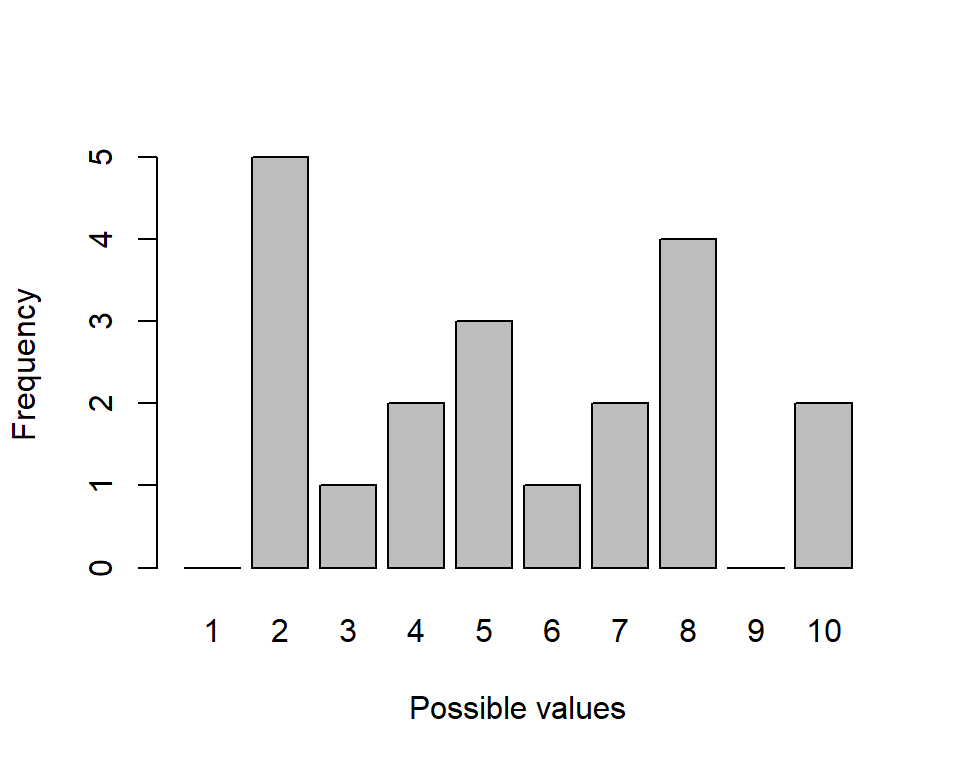
\includegraphics{IntroStats_files/figure-latex/barplot1-1} 

}

\caption{Vertical bar chart representing the frequency distribution in Table 1.}\label{fig:barplot1}
\end{figure}

In Figure \ref{fig:barplot1}, the bars are vertical but they could also be horizontal. The gaps between the bars are a useful reminder that the values are discrete (ane we look at histograms where there are no gaps later).

\hypertarget{pie-charts}{%
\subsection{Pie charts}\label{pie-charts}}

Pie charts are another way to view information in a frequency distribution (Figure \ref{fig:piechart1}). The area (and central angle) of each slice is proportional to the number it represents.

\begin{figure}

{\centering 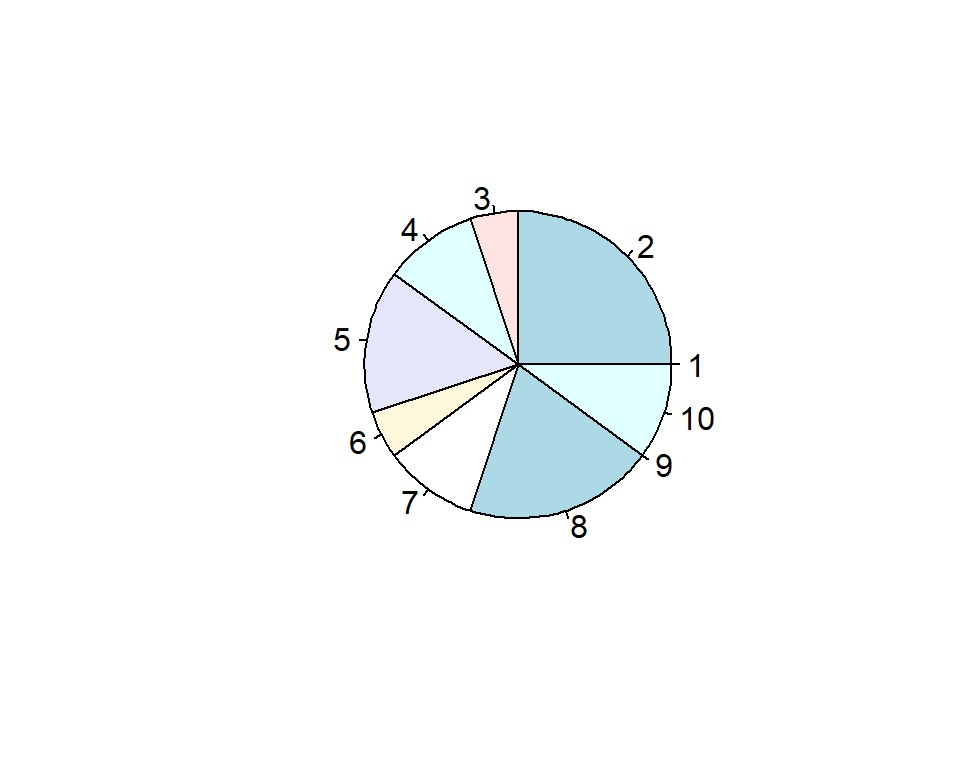
\includegraphics{IntroStats_files/figure-latex/piechart1-1} 

}

\caption{Pie chart representing the frequency distribution in Table 3.1.}\label{fig:piechart1}
\end{figure}

There are many variants of the basic pie chart (e.g.~exploded pie chart) but, in general, pie charts come with a serious `health-warning' because they can be difficult to interpret, particularly if there are many possible values.

\hypertarget{histograms}{%
\subsection{Histograms}\label{histograms}}

Histograms are a simple, effective and useful tool for displaying continuous data. Histograms partition the data values into distinct bins, or intervals, and the height of the bin represents the number of values in each bin. The division of data into different bins can alter the appearance appreciably; computer software generally have algorithms to decide on the bins (Figure \ref{fig:hist1}).

\begin{figure}

{\centering 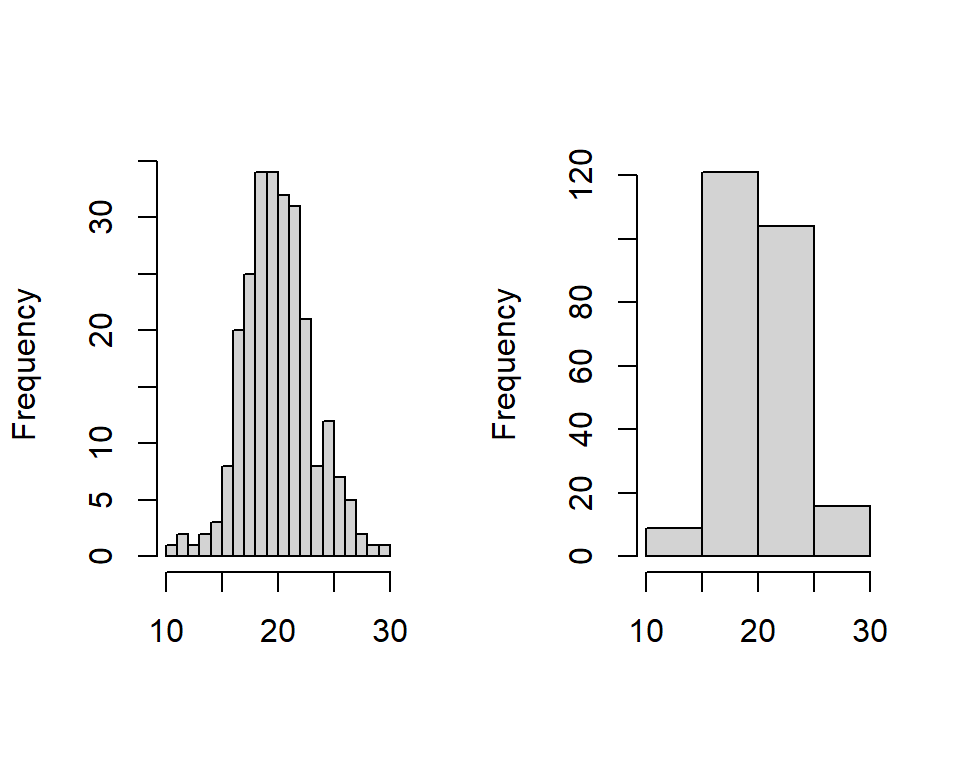
\includegraphics{IntroStats_files/figure-latex/hist1-1} 

}

\caption{Examples of data that is symmetrical about the mean is represented by two histograms using different bin widths.}\label{fig:hist1}
\end{figure}

Histograms show the \textbf{centre}, \textbf{spread} (variability) and \textbf{skewness} in the data.

\textbf{Skewness} is a measure of asymmetry about the mean and this feature is swiftly evident from histograms. In Figure \ref{fig:hist1}, 100 values are represented and the mean of the values is 20. We can see that the plot is roughly symmetric about the mean and so the skewness value is low. The median is the point where 50\% of the area of the histogram lies to the left and 50\% lies to the right. In this figure, the median is 20 - the mean and median are the same. This is always the case if the shape of the histogram is symmetric. In fact, comparing the mean and median gives an indication of the skewness of data (Figure \ref{fig:hist2}):

\begin{itemize}
\item
  Right, or positively, skewed data has a relatively long right tail compared to the left and the mean is greater than the median
\item
  Left, or negatively, skewed data has a relatively long left tail compared to the left and the mean is less than the median.
\item
  For symmetric data, the mean and median are equal.
\end{itemize}

\begin{figure}

{\centering 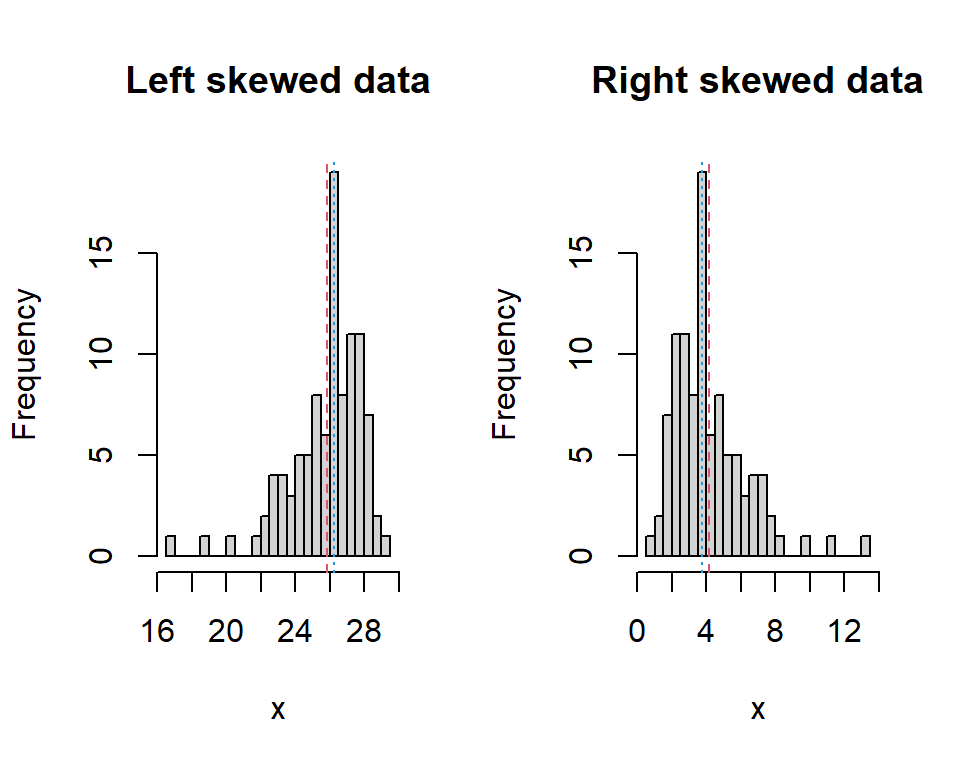
\includegraphics{IntroStats_files/figure-latex/hist2-1} 

}

\caption{Histograms of left-skewed data and right-skewed data. The red dashed line indicates the mean and the blue dotted indicates the median.}\label{fig:hist2}
\end{figure}

For highly skewed data the median is often a more appropriate measure of the centre than the mean, for example, salary or house prices.

A histogram is useful because it shows the sampled frequency of different ranges of values. If there is no discernible peak (or peaks) and all values are similarly likely, the distribution is described as uniform (Figure \ref{fig:hist3}).

\begin{figure}

{\centering 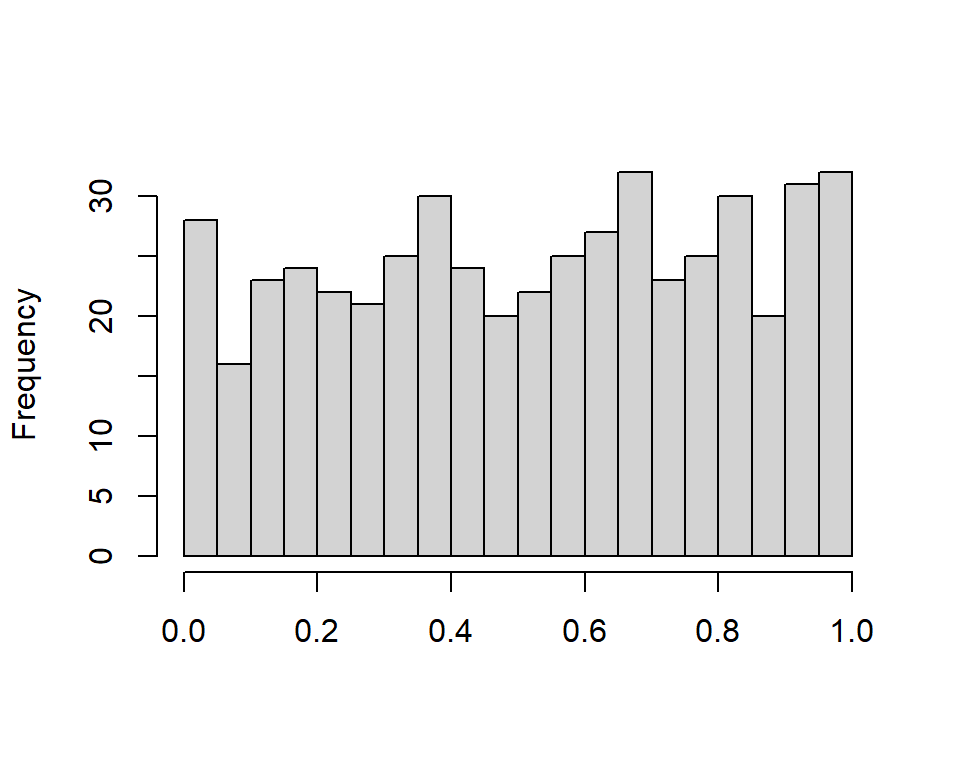
\includegraphics{IntroStats_files/figure-latex/hist3-1} 

}

\caption{A histogram showing 500 values selected at random from the set [0, 1].}\label{fig:hist3}
\end{figure}

\hypertarget{boxplots}{%
\subsection{Boxplots}\label{boxplots}}

An alternative to the histogram is the box plot (or box-and-whisker plot). These plots convey summary numerical information in the plot (Figure \ref{fig:boxplot1})

\begin{figure}

{\centering 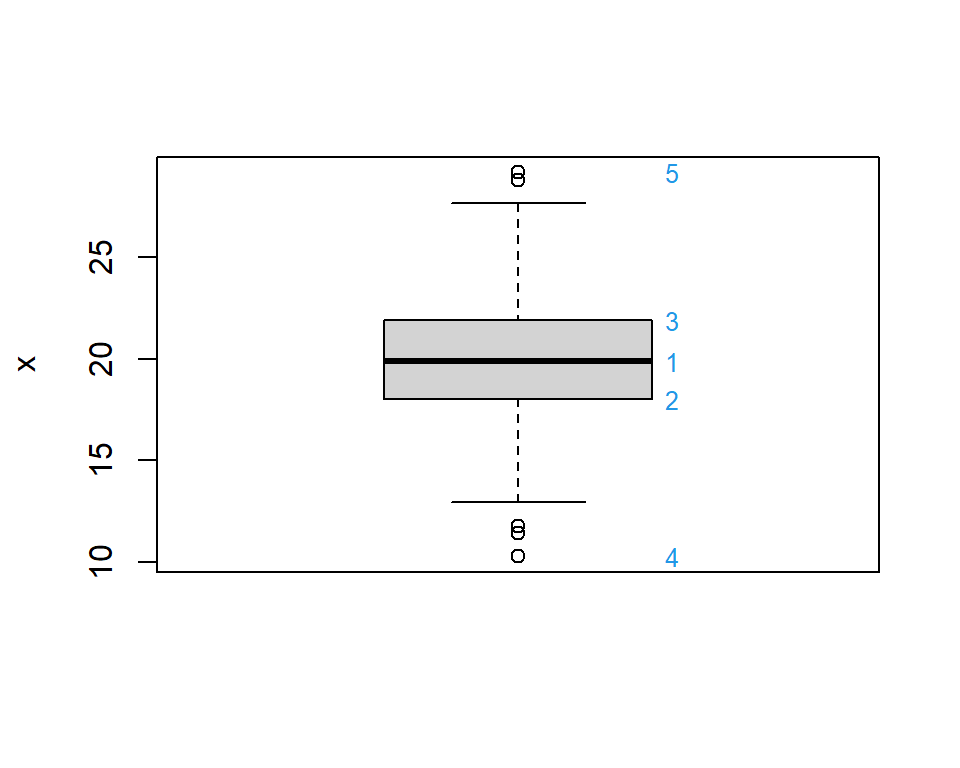
\includegraphics{IntroStats_files/figure-latex/boxplot1-1} 

}

\caption{Box plot of 100 values of variable called $x$. See below for an explanation of the numbers in blue.}\label{fig:boxplot1}
\end{figure}

The following numerical information can be gleaned from the plot (which was obtained in R using the default values):

\begin{itemize}
\item
  the median of the data is represented by the thick black line across the box (\color{blue}1 \color{black} on Figure \ref{fig:boxplot1}),
\item
  the lower limit of the box is the 25th percentile (\color{blue}2\color{black}),
\item
  the upper limit of the box is the 75th percentile (\color{blue}3\color{black}),
\item
  the height of the box spans the IQR,
\item
  the `whiskers' extend to the most extreme values, as long as these values are no more than 1.5 \(\times\) the IQR from the box (this can be changed in R),
\item
  if there are any values beyond the whiskers (as there are in Figure \ref{fig:boxplot1}), they are plotted as dots and highlighted as potentially unusual points (\color{blue}4 \color{black} and \color{blue}5\color{black}).
\end{itemize}

\hypertarget{basic-plots-in-r}{%
\subsection{Basic plots in R}\label{basic-plots-in-r}}

To create examples of the above plots in R, first some data is generated - stored in an object called \(x\). Don't worry at present about the command used to create the data - this will be addressed later in the course.

\begin{Shaded}
\begin{Highlighting}[]
\CommentTok{\# Set seed for RNG}
\FunctionTok{set.seed}\NormalTok{(}\DecValTok{1234}\NormalTok{)}
\CommentTok{\# Generate 100 random values from a symmetric (normal) distribution with}
\CommentTok{\#   mean=20 and standard deviation=3}
\NormalTok{x }\OtherTok{\textless{}{-}} \FunctionTok{rnorm}\NormalTok{(}\AttributeTok{n=}\DecValTok{100}\NormalTok{, }\AttributeTok{mean=}\DecValTok{20}\NormalTok{, }\AttributeTok{sd=}\DecValTok{3}\NormalTok{)}

\CommentTok{\# Boxplot}
\FunctionTok{boxplot}\NormalTok{(x)}
\end{Highlighting}
\end{Shaded}

\begin{center}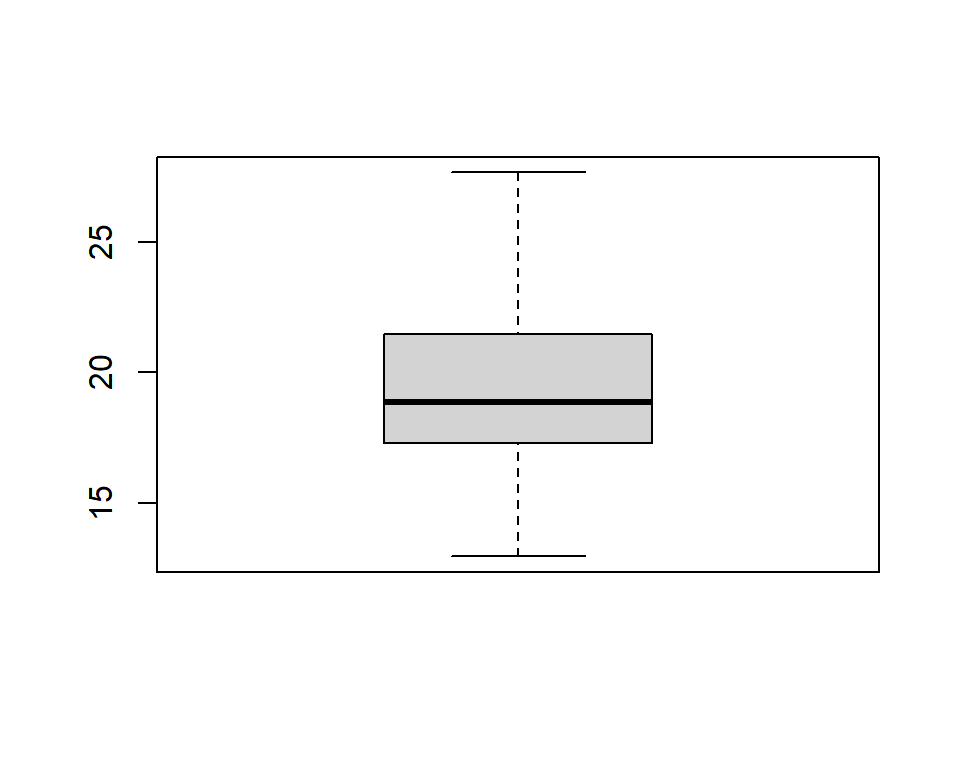
\includegraphics{IntroStats_files/figure-latex/unnamed-chunk-11-1} \end{center}

\begin{Shaded}
\begin{Highlighting}[]
\CommentTok{\# Histogram}
\FunctionTok{hist}\NormalTok{(x)}
\end{Highlighting}
\end{Shaded}

\begin{center}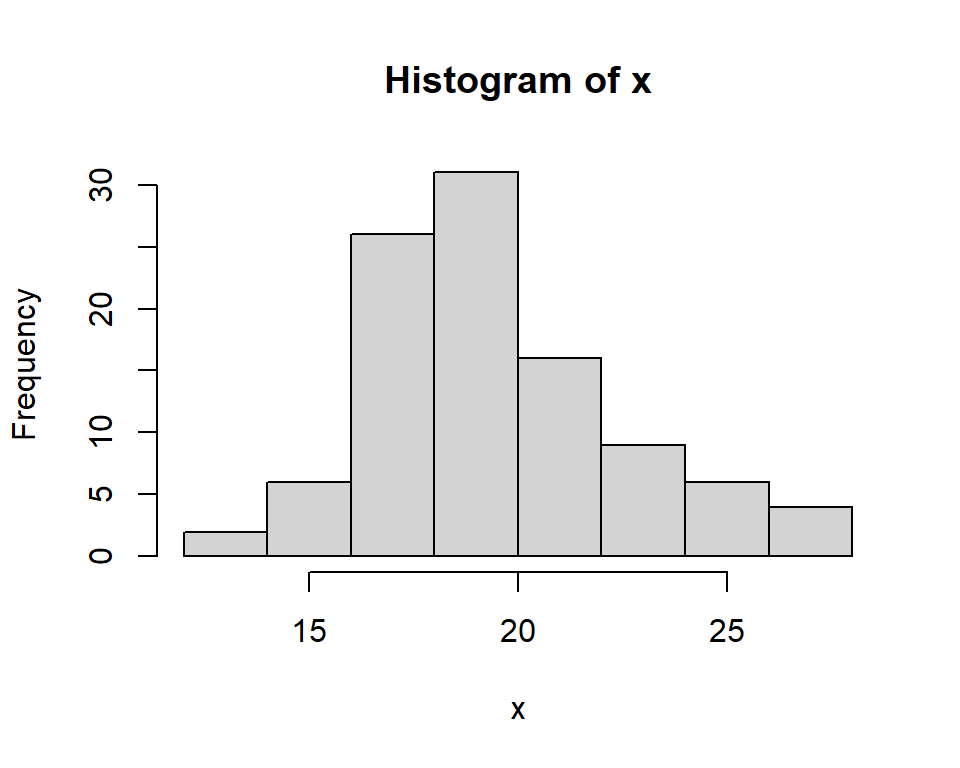
\includegraphics{IntroStats_files/figure-latex/unnamed-chunk-11-2} \end{center}

\begin{Shaded}
\begin{Highlighting}[]
\CommentTok{\# Create more bins (note the number of bins may not be exactly that specified)}
\FunctionTok{hist}\NormalTok{(x, }\AttributeTok{nclass=}\DecValTok{10}\NormalTok{, }\AttributeTok{main=}\StringTok{"Histogram of x with more bins"}\NormalTok{)}
\end{Highlighting}
\end{Shaded}

\begin{center}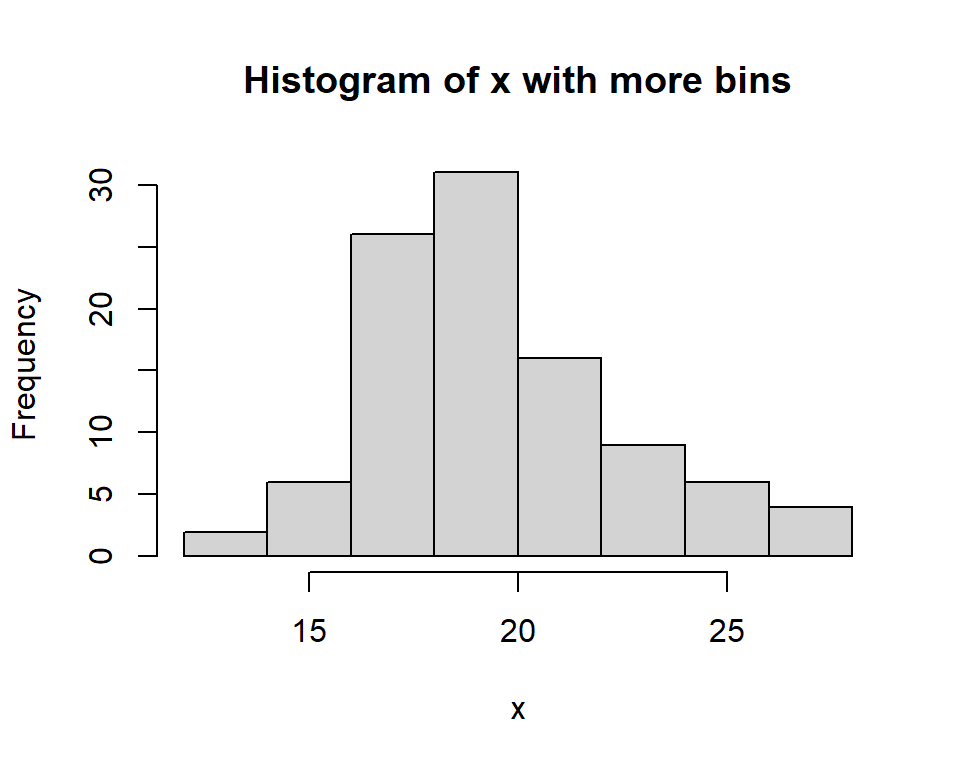
\includegraphics{IntroStats_files/figure-latex/unnamed-chunk-11-3} \end{center}

\begin{Shaded}
\begin{Highlighting}[]
\CommentTok{\# Use specific bin intervals}
\NormalTok{bins }\OtherTok{\textless{}{-}} \FunctionTok{seq}\NormalTok{(}\AttributeTok{from=}\DecValTok{10}\NormalTok{, }\AttributeTok{to=}\DecValTok{30}\NormalTok{, }\AttributeTok{by=}\DecValTok{2}\NormalTok{)}
\NormalTok{bins}
\end{Highlighting}
\end{Shaded}

\begin{verbatim}
 [1] 10 12 14 16 18 20 22 24 26 28 30
\end{verbatim}

\begin{Shaded}
\begin{Highlighting}[]
\FunctionTok{hist}\NormalTok{(x, }\AttributeTok{breaks=}\NormalTok{bins)}
\end{Highlighting}
\end{Shaded}

\begin{center}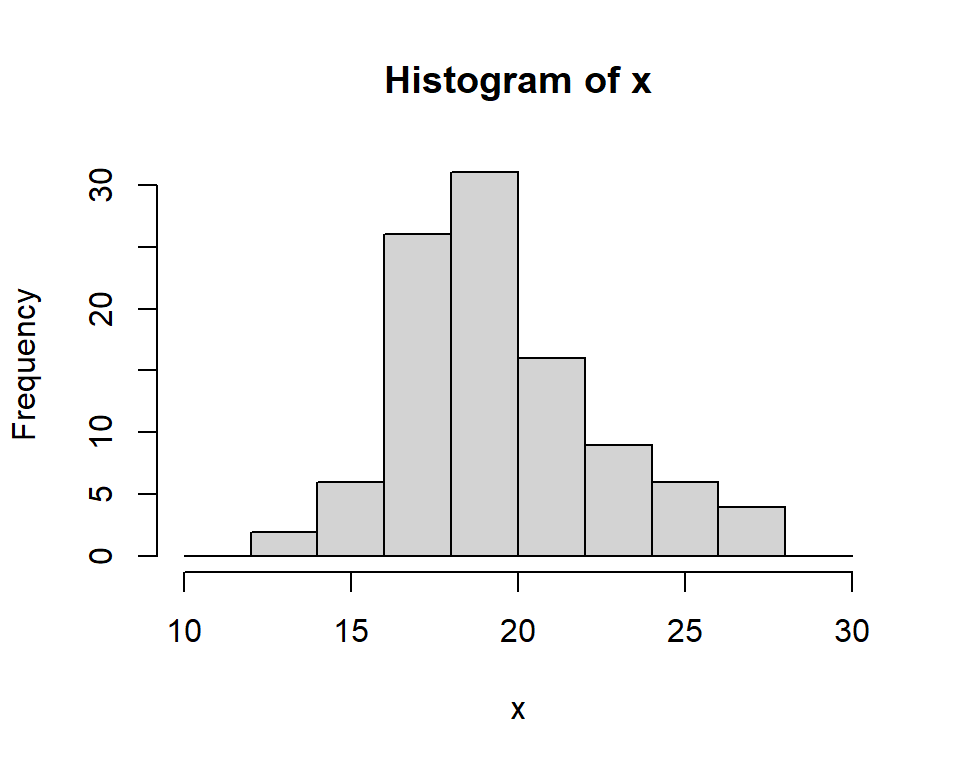
\includegraphics{IntroStats_files/figure-latex/unnamed-chunk-11-4} \end{center}

\hypertarget{other-plots}{%
\subsection{Other plots}\label{other-plots}}

Histograms and box plots are classical plots but more sophisticated plots have been developed more recently which can be used as alternatives, such as the \href{https://mode.com/blog/violin-plot-examples/}{violin plot} and \href{https://micahallen.org/2018/03/15/introducing-raincloud-plots/}{rain cloud plots}. Both combine box plots and a smoothed histogram.

\hypertarget{summarising-the-relationship-between-two-variables}{%
\section{Summarising the relationship between two variables}\label{summarising-the-relationship-between-two-variables}}

The plots and numerical summaries described so far have been concerned with a single variable. Frequently, we want to look at the relationship between two variables. In many situations one variable (conventionally denoted by \(X\)), will be considered as an explanatory (or independent) variable, while the other variable (conventionally denoted by \(Y\)), is deemed to be the response (or dependent) variable. The methods used to summarise (and analyse) these data depend on the types of data (see Table \ref{tab:datareltab} for some examples).

\begin{longtable}[]{@{}cccc@{}}
\caption{\label{tab:datareltab} Examples of the relationship between different types of data.}\tabularnewline
\toprule
\begin{minipage}[b]{(\columnwidth - 3\tabcolsep) * \real{0.31}}\centering
X\strut
\end{minipage} & \begin{minipage}[b]{(\columnwidth - 3\tabcolsep) * \real{0.28}}\centering
Y\strut
\end{minipage} & \begin{minipage}[b]{(\columnwidth - 3\tabcolsep) * \real{0.20}}\centering
X.type\strut
\end{minipage} & \begin{minipage}[b]{(\columnwidth - 3\tabcolsep) * \real{0.20}}\centering
Y.type\strut
\end{minipage}\tabularnewline
\midrule
\endfirsthead
\toprule
\begin{minipage}[b]{(\columnwidth - 3\tabcolsep) * \real{0.31}}\centering
X\strut
\end{minipage} & \begin{minipage}[b]{(\columnwidth - 3\tabcolsep) * \real{0.28}}\centering
Y\strut
\end{minipage} & \begin{minipage}[b]{(\columnwidth - 3\tabcolsep) * \real{0.20}}\centering
X.type\strut
\end{minipage} & \begin{minipage}[b]{(\columnwidth - 3\tabcolsep) * \real{0.20}}\centering
Y.type\strut
\end{minipage}\tabularnewline
\midrule
\endhead
\begin{minipage}[t]{(\columnwidth - 3\tabcolsep) * \real{0.31}}\centering
Amount of fertilizer\strut
\end{minipage} & \begin{minipage}[t]{(\columnwidth - 3\tabcolsep) * \real{0.28}}\centering
Weight of Crop\strut
\end{minipage} & \begin{minipage}[t]{(\columnwidth - 3\tabcolsep) * \real{0.20}}\centering
Quantitative\strut
\end{minipage} & \begin{minipage}[t]{(\columnwidth - 3\tabcolsep) * \real{0.20}}\centering
Quantitative\strut
\end{minipage}\tabularnewline
\begin{minipage}[t]{(\columnwidth - 3\tabcolsep) * \real{0.31}}\centering
Gender\strut
\end{minipage} & \begin{minipage}[t]{(\columnwidth - 3\tabcolsep) * \real{0.28}}\centering
Salary\strut
\end{minipage} & \begin{minipage}[t]{(\columnwidth - 3\tabcolsep) * \real{0.20}}\centering
Qualitative\strut
\end{minipage} & \begin{minipage}[t]{(\columnwidth - 3\tabcolsep) * \real{0.20}}\centering
Quantitative\strut
\end{minipage}\tabularnewline
\begin{minipage}[t]{(\columnwidth - 3\tabcolsep) * \real{0.31}}\centering
Socio/economic class\strut
\end{minipage} & \begin{minipage}[t]{(\columnwidth - 3\tabcolsep) * \real{0.28}}\centering
Type of employment\strut
\end{minipage} & \begin{minipage}[t]{(\columnwidth - 3\tabcolsep) * \real{0.20}}\centering
Qualitative\strut
\end{minipage} & \begin{minipage}[t]{(\columnwidth - 3\tabcolsep) * \real{0.20}}\centering
Qualitative\strut
\end{minipage}\tabularnewline
\bottomrule
\end{longtable}

\hypertarget{cross-tabulation}{%
\subsection{Cross-tabulation}\label{cross-tabulation}}

If both variables are qualitative, or discrete with a small number of possible values, then a cross-tabulation (also known as a contingency table) could be used - this is essentially an extension of the frequency distribution seen previously.

Table \ref{tab:dietdatatab} is an example of a cross-tabulation which summarises the number of people using one of three diets by gender.

\begin{longtable}[]{@{}cccc@{}}
\caption{\label{tab:dietdatatab} Number of subjects by diet and gender.}\tabularnewline
\toprule
\begin{minipage}[b]{(\columnwidth - 3\tabcolsep) * \real{0.19}}\centering
~\strut
\end{minipage} & \begin{minipage}[b]{(\columnwidth - 3\tabcolsep) * \real{0.07}}\centering
1\strut
\end{minipage} & \begin{minipage}[b]{(\columnwidth - 3\tabcolsep) * \real{0.07}}\centering
2\strut
\end{minipage} & \begin{minipage}[b]{(\columnwidth - 3\tabcolsep) * \real{0.07}}\centering
3\strut
\end{minipage}\tabularnewline
\midrule
\endfirsthead
\toprule
\begin{minipage}[b]{(\columnwidth - 3\tabcolsep) * \real{0.19}}\centering
~\strut
\end{minipage} & \begin{minipage}[b]{(\columnwidth - 3\tabcolsep) * \real{0.07}}\centering
1\strut
\end{minipage} & \begin{minipage}[b]{(\columnwidth - 3\tabcolsep) * \real{0.07}}\centering
2\strut
\end{minipage} & \begin{minipage}[b]{(\columnwidth - 3\tabcolsep) * \real{0.07}}\centering
3\strut
\end{minipage}\tabularnewline
\midrule
\endhead
\begin{minipage}[t]{(\columnwidth - 3\tabcolsep) * \real{0.19}}\centering
\textbf{Female}\strut
\end{minipage} & \begin{minipage}[t]{(\columnwidth - 3\tabcolsep) * \real{0.07}}\centering
14\strut
\end{minipage} & \begin{minipage}[t]{(\columnwidth - 3\tabcolsep) * \real{0.07}}\centering
14\strut
\end{minipage} & \begin{minipage}[t]{(\columnwidth - 3\tabcolsep) * \real{0.07}}\centering
15\strut
\end{minipage}\tabularnewline
\begin{minipage}[t]{(\columnwidth - 3\tabcolsep) * \real{0.19}}\centering
\textbf{Male}\strut
\end{minipage} & \begin{minipage}[t]{(\columnwidth - 3\tabcolsep) * \real{0.07}}\centering
10\strut
\end{minipage} & \begin{minipage}[t]{(\columnwidth - 3\tabcolsep) * \real{0.07}}\centering
11\strut
\end{minipage} & \begin{minipage}[t]{(\columnwidth - 3\tabcolsep) * \real{0.07}}\centering
12\strut
\end{minipage}\tabularnewline
\begin{minipage}[t]{(\columnwidth - 3\tabcolsep) * \real{0.19}}\centering
\textbf{Unknown}\strut
\end{minipage} & \begin{minipage}[t]{(\columnwidth - 3\tabcolsep) * \real{0.07}}\centering
0\strut
\end{minipage} & \begin{minipage}[t]{(\columnwidth - 3\tabcolsep) * \real{0.07}}\centering
2\strut
\end{minipage} & \begin{minipage}[t]{(\columnwidth - 3\tabcolsep) * \real{0.07}}\centering
0\strut
\end{minipage}\tabularnewline
\bottomrule
\end{longtable}

\hypertarget{doing-this-in-r-3}{%
\subsubsection{Doing this in R}\label{doing-this-in-r-3}}

\begin{Shaded}
\begin{Highlighting}[]
\CommentTok{\# Example of a cross{-}tabulation}
\CommentTok{\# Create some data {-} specify sample size}
\NormalTok{n }\OtherTok{\textless{}{-}} \DecValTok{10}
\CommentTok{\# Generate values at random}
\NormalTok{var1 }\OtherTok{\textless{}{-}} \FunctionTok{sample}\NormalTok{(}\DecValTok{1}\SpecialCharTok{:}\DecValTok{5}\NormalTok{, }\AttributeTok{size=}\NormalTok{n, }\AttributeTok{replace=}\ConstantTok{TRUE}\NormalTok{)}
\NormalTok{var2 }\OtherTok{\textless{}{-}} \FunctionTok{sample}\NormalTok{(}\FunctionTok{c}\NormalTok{(}\StringTok{"Y"}\NormalTok{,}\StringTok{"N"}\NormalTok{), }\AttributeTok{size=}\NormalTok{n, }\AttributeTok{replace=}\ConstantTok{TRUE}\NormalTok{)}
\CommentTok{\# Print data}
\NormalTok{var1}
\end{Highlighting}
\end{Shaded}

\begin{verbatim}
 [1] 3 3 5 1 4 4 3 2 1 1
\end{verbatim}

\begin{Shaded}
\begin{Highlighting}[]
\NormalTok{var2}
\end{Highlighting}
\end{Shaded}

\begin{verbatim}
 [1] "Y" "N" "Y" "Y" "Y" "N" "N" "N" "Y" "Y"
\end{verbatim}

\begin{Shaded}
\begin{Highlighting}[]
\CommentTok{\# Cross tabulation of data}
\FunctionTok{table}\NormalTok{(var1, var2)}
\end{Highlighting}
\end{Shaded}

\begin{verbatim}
    var2
var1 N Y
   1 0 3
   2 1 0
   3 2 1
   4 1 1
   5 0 1
\end{verbatim}

\hypertarget{side-by-side-boxplots}{%
\subsection{Side-by-side boxplots}\label{side-by-side-boxplots}}

If one variable is discrete and one continuous, then the continuous data could be divided into the groups specified by the qualitative (or discrete) variable: a numerical summary and box plot can be created for each group. For example in Figure \ref{fig:boxplot2}, the initial weights of people using one of three diets are illustrated.

\begin{figure}

{\centering 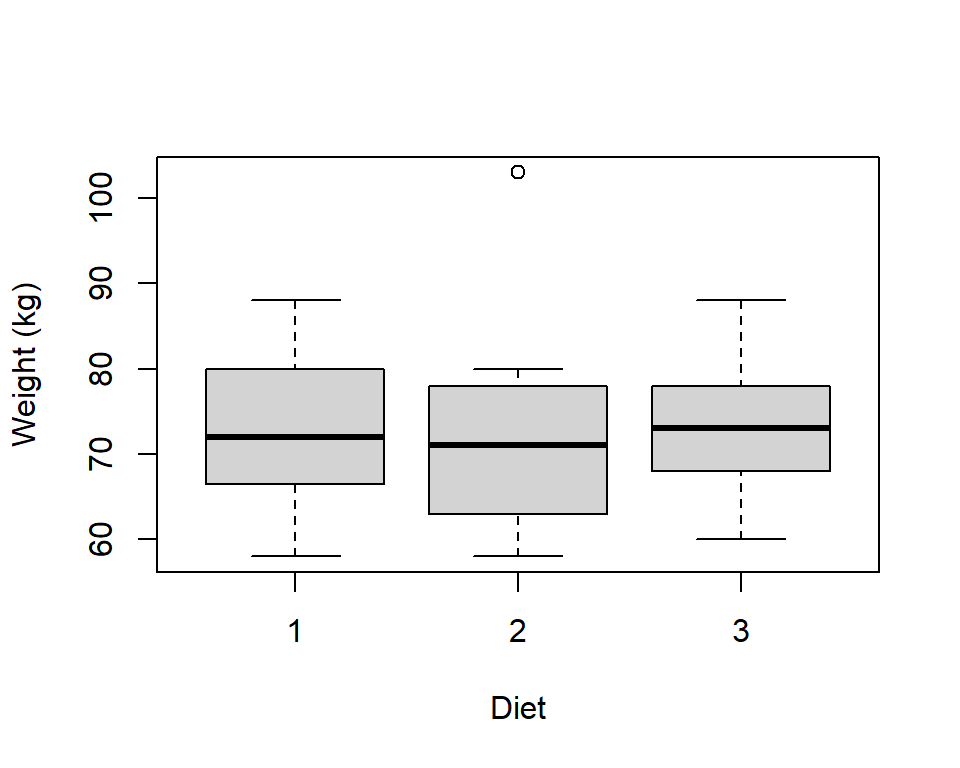
\includegraphics{IntroStats_files/figure-latex/boxplot2-1} 

}

\caption{Example of side-by-side boxplots to display the relationship between a quantitative and a qualitative variable.}\label{fig:boxplot2}
\end{figure}

Histograms could also be used in a similar way - see the computer practical associated with this chapter.

\hypertarget{scatter-plot}{%
\subsection{Scatter plot}\label{scatter-plot}}

The scatter plot is frequently used to display the relationship between two continuous variables. The values for each pair of variables are plotted on a graph with the response on the \(y\)-axis and the explanatory variable on the \(x\)-axis (Figure \ref{fig:scatter1}).

\begin{figure}

{\centering 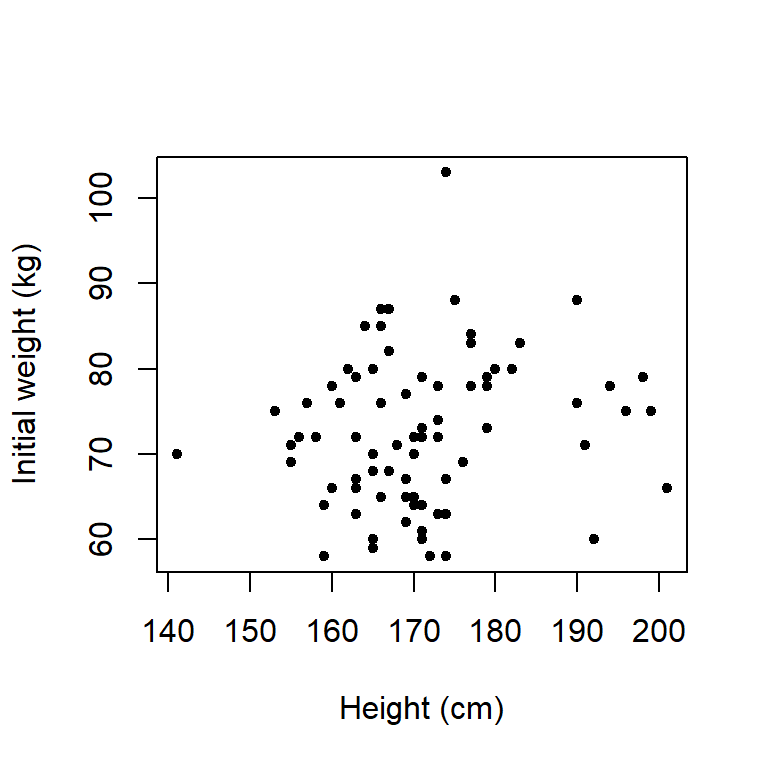
\includegraphics{IntroStats_files/figure-latex/scatter1-1} 

}

\caption{Scatter plot showing the relationship between the height and weight of subjects before starting a diet.}\label{fig:scatter1}
\end{figure}

If there was a third, discrete variable, then different colours, or symbols, could be used to highlight the points for the different levels. For example, in Figure \ref{fig:scatter2} the different coloured and shaped symbols represent the diet.

\begin{figure}

{\centering 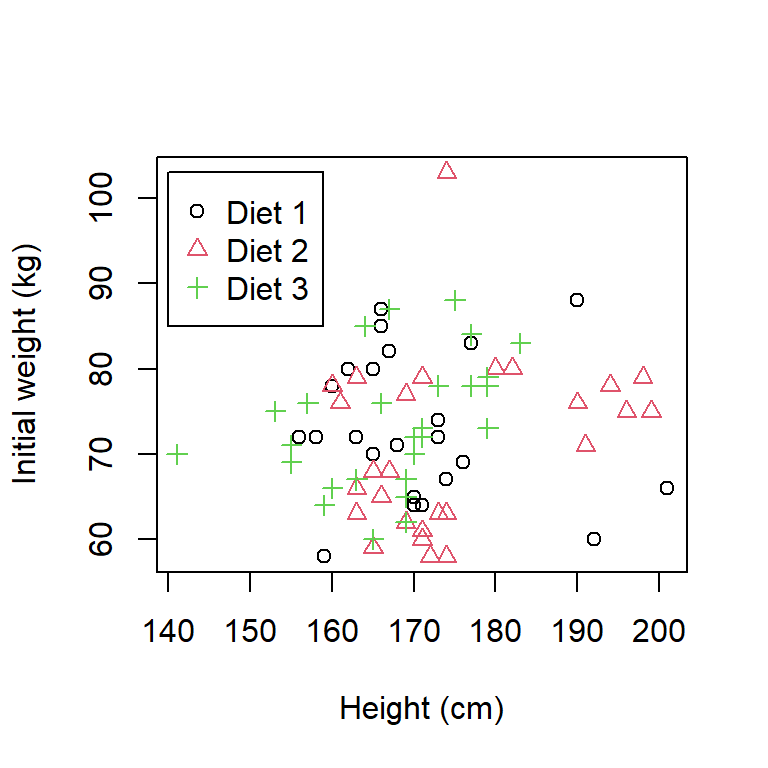
\includegraphics{IntroStats_files/figure-latex/scatter2-1} 

}

\caption{Scatter plot of the height and weight of subjects indicating diet group.}\label{fig:scatter2}
\end{figure}

\textit{Are there any obvious relationships in these data?}

\begin{itemize}
\item
  The initial weights seem to be fairly similar across each group (see point below).
\item
  The range of heights in each group is approximately 45cm but for diet groups 1 and 2, the minimum and maximum heights are 155 and 200cm approximately, whereas in the diet 3 group, the minimum and maximum are 141 and 185cm approx.
\item
  There are two observations that are potentially unusual; one height is substantially smaller that other heights (approx. 141 cm) and one weight is substantially larger that other weights (approx. 103 kg).
\end{itemize}

\hypertarget{doing-this-in-r-4}{%
\subsubsection{Doing this in R}\label{doing-this-in-r-4}}

To illustrate how to create a scatter plot in R, we first need to create some data. Don't worry too much about the commands used to create the data - these will be explained further as we go through the course. The more important commands for this section are the plot commands.

\begin{Shaded}
\begin{Highlighting}[]
\CommentTok{\# Generate 50 random values between 10 and 50}
\NormalTok{num }\OtherTok{\textless{}{-}} \DecValTok{50}
\NormalTok{xdata }\OtherTok{\textless{}{-}} \FunctionTok{runif}\NormalTok{(}\AttributeTok{n=}\NormalTok{num, }\AttributeTok{min=}\DecValTok{10}\NormalTok{, }\AttributeTok{max=}\DecValTok{50}\NormalTok{)}
\CommentTok{\# Generate 50 random values from a normal distribution (mean=x and sd=5)}
\NormalTok{ydata }\OtherTok{\textless{}{-}} \FunctionTok{rnorm}\NormalTok{(}\AttributeTok{n=}\NormalTok{num, }\AttributeTok{mean=}\NormalTok{xdata, }\AttributeTok{sd=}\DecValTok{3}\NormalTok{)}

\CommentTok{\# Scatter plot}
\FunctionTok{plot}\NormalTok{(}\AttributeTok{x=}\NormalTok{xdata, }\AttributeTok{y=}\NormalTok{ydata)}
\end{Highlighting}
\end{Shaded}

\begin{center}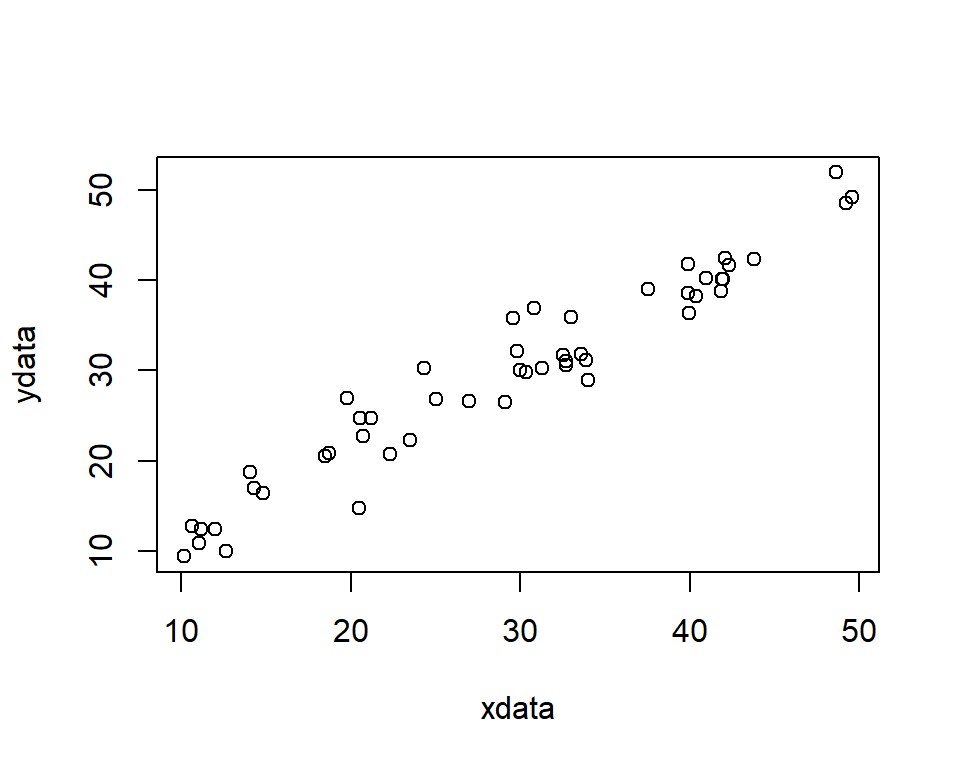
\includegraphics{IntroStats_files/figure-latex/unnamed-chunk-13-1} \end{center}

There are many options available in the \texttt{plot} functions to customise the plot, for example, different plotting symbols and colours. Use the help facility in R to look at the options available.

\hypertarget{quilt-plots}{%
\subsection{Quilt plots}\label{quilt-plots}}

If we are interested in the relationship between three continuous variables, a quilt plot can be used (an application can be found here \href{https://europepmc.org/article/med/24454789}{here}). These are a particularly useful way to summarise geo-referenced data (e.g.~where variables \(x\) and \(y\) represent spatial coordinates and a third variable \(z\) may represent altitude, for example).

\textbf{Q3.3} A doctor is investigating the effects of exercise on arthritis in human subjects aged 60 years. One hundred arthritis sufferers and 100 people who do not suffer from arthritis are asked to estimate how many hours of exercise they have taken each week, on average, over the past 5 years. The distribution of the average number of hours of exercise taken per week per person (called \(X\)) for both groups is shown in the histogram below. Based on the figure which statement is certainly FALSE (pick one statement only).

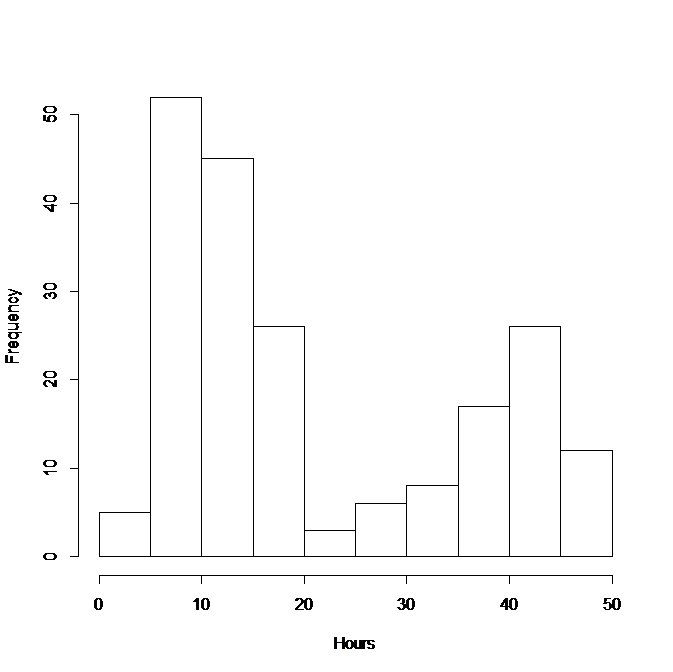
\includegraphics{figures/Bimodal_histogram.png}

A The minimum value of the data is 2 and the maximum value is 50 hours.

B The first, or lower, quartile lies in the range 0 to 10.

C The median lies in the range 20 to 30.

D The mean is 21.1 hours.

\textbf{Q3.4} \textbf{a.} The following numbers were generated with the function \texttt{fivenum}. What are the range and IQR?

\begin{verbatim}
[1]  8.271511 15.028300 17.323850 19.924308 32.079176
\end{verbatim}

\textbf{b.} A box plot was also provided and shown below. How can you tell that the box plot and five number summary are not describing exactly the same observations?

\begin{center}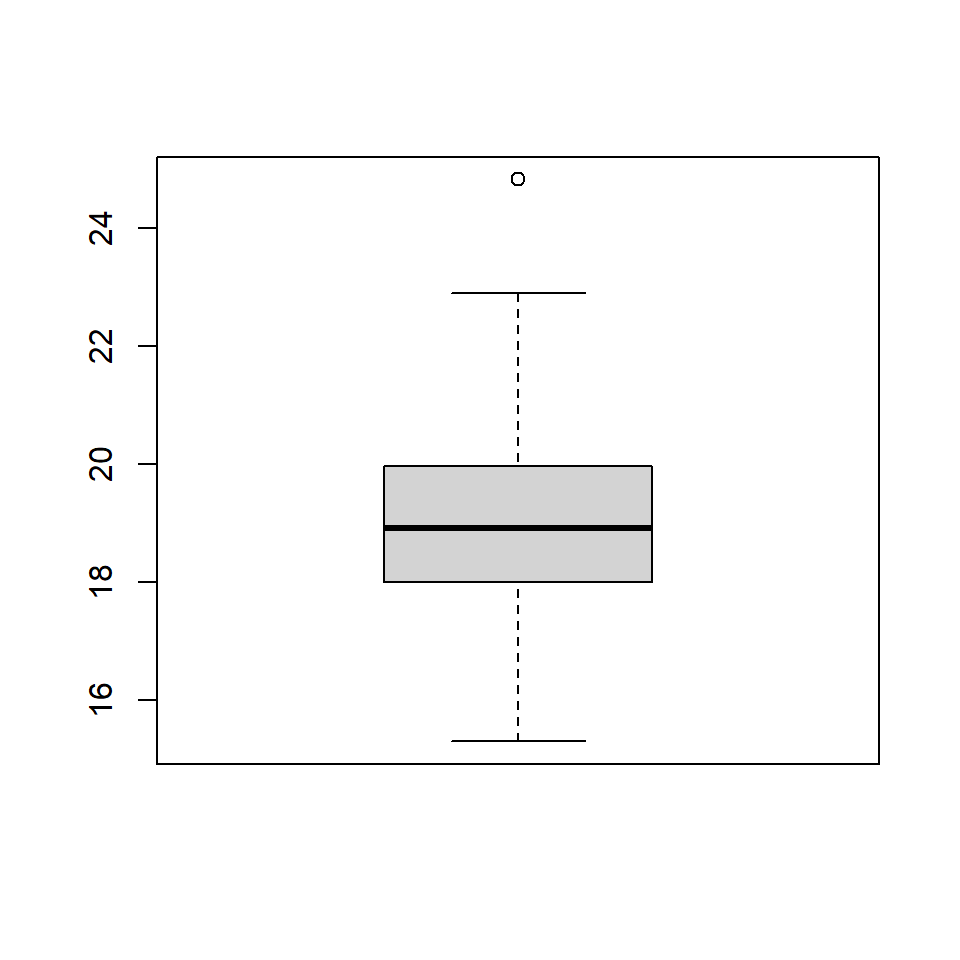
\includegraphics{IntroStats_files/figure-latex/unnamed-chunk-15-1} \end{center}

\textbf{Q3.5} What is the difference between a bar chart and a histogram?

\textbf{Q3.6} Consider the following summary of a continuous variable obtained using the \texttt{summary} function in \texttt{R}. What can you tell about the distribution of this variable?

\begin{verbatim}
   Min. 1st Qu.  Median    Mean 3rd Qu.    Max. 
0.04794 0.48459 0.86375 1.04466 1.38397 5.08813 
\end{verbatim}

\textbf{Q3.7} What method would be useful to assess the relationship between the following two variables:

\begin{enumerate}
\def\labelenumi{\alph{enumi}.}
\item
  Ethnicity and type of employment (e.g.~retail, agricultural, medical).
\item
  Volume of rainfall (litres) and the amount of runoff on an airport runway (litres).
\item
  Temperature (\(^o\)C) and habitat type (e.g.~Farmland, woodland).
\end{enumerate}

\hypertarget{handy-hints-when-including-tables-and-plots-into-reports}{%
\section{Handy hints when including tables and plots into reports}\label{handy-hints-when-including-tables-and-plots-into-reports}}

When including tables and plots into reports it is useful to keep a few rules in mind so that they are easy to understand and interpret and illustrate the key points.

\textbf{Figures}

\begin{itemize}
\item
  Make the plots self-explanatory: provide a title or label, label the axes and clearly state the units, provide a key if required.
\item
  Choose a scale that is convenient and makes the most of the paper/plotting region (i.e.~does not have too much `white-space')
\item
  Include the origin, or if it is not included take care not to mislead.
\item
  Consider whether the information may be more easily understood in a table, maybe in addition to any plots.
\end{itemize}

\textbf{Tables}

\begin{itemize}
\item
  Make the table clear and simple with the main numbers for comparison close to each other.
\item
  Arrange rows and columns in some natural order.
\item
  Choose convenient units and state what they are.
\item
  Provide a title and brief explanation of the data displayed.
\item
  If the table is getting complicated, consider splitting a table into smaller tables.
\item
  Round the numbers to an appropriate number of digits for presentation, for example two effective digits (e.g.~129, 1.2) but not for calculation.
\end{itemize}

\textbf{Example} Consider Table \ref{tab:maritaltab1} showing the numbers of people aged 16 and over in Wales in 2001 by marital status.

\begin{longtable}[]{@{}cc@{}}
\caption{\label{tab:maritaltab1} Number of people in each marital status group.}\tabularnewline
\toprule
\begin{minipage}[b]{(\columnwidth - 1\tabcolsep) * \real{0.35}}\centering
Status\strut
\end{minipage} & \begin{minipage}[b]{(\columnwidth - 1\tabcolsep) * \real{0.14}}\centering
Number\strut
\end{minipage}\tabularnewline
\midrule
\endfirsthead
\toprule
\begin{minipage}[b]{(\columnwidth - 1\tabcolsep) * \real{0.35}}\centering
Status\strut
\end{minipage} & \begin{minipage}[b]{(\columnwidth - 1\tabcolsep) * \real{0.14}}\centering
Number\strut
\end{minipage}\tabularnewline
\midrule
\endhead
\begin{minipage}[t]{(\columnwidth - 1\tabcolsep) * \real{0.35}}\centering
Single (never married)\strut
\end{minipage} & \begin{minipage}[t]{(\columnwidth - 1\tabcolsep) * \real{0.14}}\centering
649512\strut
\end{minipage}\tabularnewline
\begin{minipage}[t]{(\columnwidth - 1\tabcolsep) * \real{0.35}}\centering
Married\strut
\end{minipage} & \begin{minipage}[t]{(\columnwidth - 1\tabcolsep) * \real{0.14}}\centering
1031511\strut
\end{minipage}\tabularnewline
\begin{minipage}[t]{(\columnwidth - 1\tabcolsep) * \real{0.35}}\centering
Remarried\strut
\end{minipage} & \begin{minipage}[t]{(\columnwidth - 1\tabcolsep) * \real{0.14}}\centering
172466\strut
\end{minipage}\tabularnewline
\begin{minipage}[t]{(\columnwidth - 1\tabcolsep) * \real{0.35}}\centering
Separated (but legally
married)\strut
\end{minipage} & \begin{minipage}[t]{(\columnwidth - 1\tabcolsep) * \real{0.14}}\centering
43819\strut
\end{minipage}\tabularnewline
\begin{minipage}[t]{(\columnwidth - 1\tabcolsep) * \real{0.35}}\centering
Divorced\strut
\end{minipage} & \begin{minipage}[t]{(\columnwidth - 1\tabcolsep) * \real{0.14}}\centering
200991\strut
\end{minipage}\tabularnewline
\begin{minipage}[t]{(\columnwidth - 1\tabcolsep) * \real{0.35}}\centering
Widowed\strut
\end{minipage} & \begin{minipage}[t]{(\columnwidth - 1\tabcolsep) * \real{0.14}}\centering
217631\strut
\end{minipage}\tabularnewline
\begin{minipage}[t]{(\columnwidth - 1\tabcolsep) * \real{0.35}}\centering
Total\strut
\end{minipage} & \begin{minipage}[t]{(\columnwidth - 1\tabcolsep) * \real{0.14}}\centering
2315930\strut
\end{minipage}\tabularnewline
\bottomrule
\end{longtable}

For presentation, the table has been rearranged so that the rows are in order of size of group with the largest group at the top. The percentages have been added for ease of comparison (Table \ref{tab:maritaltab2}.

\begin{longtable}[]{@{}ccc@{}}
\caption{\label{tab:maritaltab2} Number and percentage by marital status.}\tabularnewline
\toprule
\begin{minipage}[b]{(\columnwidth - 2\tabcolsep) * \real{0.35}}\centering
Status\strut
\end{minipage} & \begin{minipage}[b]{(\columnwidth - 2\tabcolsep) * \real{0.24}}\centering
Number (1000s)\strut
\end{minipage} & \begin{minipage}[b]{(\columnwidth - 2\tabcolsep) * \real{0.18}}\centering
Percentage\strut
\end{minipage}\tabularnewline
\midrule
\endfirsthead
\toprule
\begin{minipage}[b]{(\columnwidth - 2\tabcolsep) * \real{0.35}}\centering
Status\strut
\end{minipage} & \begin{minipage}[b]{(\columnwidth - 2\tabcolsep) * \real{0.24}}\centering
Number (1000s)\strut
\end{minipage} & \begin{minipage}[b]{(\columnwidth - 2\tabcolsep) * \real{0.18}}\centering
Percentage\strut
\end{minipage}\tabularnewline
\midrule
\endhead
\begin{minipage}[t]{(\columnwidth - 2\tabcolsep) * \real{0.35}}\centering
Married\strut
\end{minipage} & \begin{minipage}[t]{(\columnwidth - 2\tabcolsep) * \real{0.24}}\centering
1032\strut
\end{minipage} & \begin{minipage}[t]{(\columnwidth - 2\tabcolsep) * \real{0.18}}\centering
44.5\strut
\end{minipage}\tabularnewline
\begin{minipage}[t]{(\columnwidth - 2\tabcolsep) * \real{0.35}}\centering
Single (never married)\strut
\end{minipage} & \begin{minipage}[t]{(\columnwidth - 2\tabcolsep) * \real{0.24}}\centering
650\strut
\end{minipage} & \begin{minipage}[t]{(\columnwidth - 2\tabcolsep) * \real{0.18}}\centering
28.0\strut
\end{minipage}\tabularnewline
\begin{minipage}[t]{(\columnwidth - 2\tabcolsep) * \real{0.35}}\centering
Widowed\strut
\end{minipage} & \begin{minipage}[t]{(\columnwidth - 2\tabcolsep) * \real{0.24}}\centering
218\strut
\end{minipage} & \begin{minipage}[t]{(\columnwidth - 2\tabcolsep) * \real{0.18}}\centering
9.4\strut
\end{minipage}\tabularnewline
\begin{minipage}[t]{(\columnwidth - 2\tabcolsep) * \real{0.35}}\centering
Divorced\strut
\end{minipage} & \begin{minipage}[t]{(\columnwidth - 2\tabcolsep) * \real{0.24}}\centering
201\strut
\end{minipage} & \begin{minipage}[t]{(\columnwidth - 2\tabcolsep) * \real{0.18}}\centering
8.7\strut
\end{minipage}\tabularnewline
\begin{minipage}[t]{(\columnwidth - 2\tabcolsep) * \real{0.35}}\centering
Remarried\strut
\end{minipage} & \begin{minipage}[t]{(\columnwidth - 2\tabcolsep) * \real{0.24}}\centering
172\strut
\end{minipage} & \begin{minipage}[t]{(\columnwidth - 2\tabcolsep) * \real{0.18}}\centering
7.4\strut
\end{minipage}\tabularnewline
\begin{minipage}[t]{(\columnwidth - 2\tabcolsep) * \real{0.35}}\centering
Separated (but legally
married)\strut
\end{minipage} & \begin{minipage}[t]{(\columnwidth - 2\tabcolsep) * \real{0.24}}\centering
44\strut
\end{minipage} & \begin{minipage}[t]{(\columnwidth - 2\tabcolsep) * \real{0.18}}\centering
1.9\strut
\end{minipage}\tabularnewline
\begin{minipage}[t]{(\columnwidth - 2\tabcolsep) * \real{0.35}}\centering
Total\strut
\end{minipage} & \begin{minipage}[t]{(\columnwidth - 2\tabcolsep) * \real{0.24}}\centering
2316\strut
\end{minipage} & \begin{minipage}[t]{(\columnwidth - 2\tabcolsep) * \real{0.18}}\centering
100.0\strut
\end{minipage}\tabularnewline
\bottomrule
\end{longtable}

\hypertarget{SUMdata}{%
\section{Summary}\label{SUMdata}}

Numerical summaries provide:

\begin{itemize}
\item
  a measure of the centre of the distribution (mean, median, mode),
\item
  a measure of the spead (range, IQR, standard deviation).
\end{itemize}

Histograms and box plots show overall features in the data such as the:

\begin{itemize}
\item
  mode,
\item
  symmetry or asymmetry, and
\item
  outliers.
\end{itemize}

Scatter plots show

\begin{itemize}
\item
  any relationships between the two variables
\item
  if there is a relationship, whether the relationship is linear or not, and
\item
  outliers.
\end{itemize}

\hypertarget{learning-outcomes}{%
\subsection{Learning outcomes}\label{learning-outcomes}}

You should be able to

\begin{enumerate}
\def\labelenumi{\arabic{enumi}.}
\item
  recognise different types of data
\item
  calculate a numerical summery of the centre and spread for a set of data
\item
  choose an appropriate plot and understand the features of the different plots.
\end{enumerate}

\hypertarget{ANSdata}{%
\section{Answers}\label{ANSdata}}

\textbf{Q3.1} The five numbers produced by the \texttt{fivenum} function are minimum, 25th percentile, median, 75th percentile and maximum (in that order). Note, the difference in the percentile measurements between \texttt{fivenum} and \texttt{summary} functions; \texttt{summary} uses a different algorithm to calculate the percentiles. The `help' for \texttt{fivenum} refers to a lower-hinge and an upper-hinge, these are the 25th and 75th percentiles, respectively.

\textbf{Q3.2} \textbf{a.} The mean is given by

\[ \bar x = \frac{\sum_{i=1}^{n} {x_i}}n=\frac{19.5 + 9.8 + 8.6 + 11.5 + 5.1}5 = \frac{54.4}5 = 10.9 \]

\textbf{Q3.2} \textbf{b.} To calculate the median, we need to first sort the data in numerical order; \{5.1, 8.6, 9.8, 11.5, 19.5\}. The median is the value at\(\textrm{position} =\frac{5+1}2 = 3\). The value in the 3rd position is 9.8, hence, this is the median.

\textbf{Q3.2} \textbf{c.} The range is given by the maximum - minimum value which is \(19.5 - 5.1 = 14.1\).

\textbf{Q3.2} \textbf{d.} The sample standard deviation is given by:

\[s = \sqrt{\frac{\sum_{i=1}^n{(x_i - \bar x)^2}}{n-1}} \]

\[s = \sqrt{\frac{(5.1-10.9)^2 + (8.6-10.9)^2 + (9.8-10.9)^2 + (11.5-10.9)^2 + (19.5-10.9)^2}{5-1}}\]

\[   = \sqrt{\frac{73.96 + 1.21 + 5.29 + 0.36 + 33.64}{4}} = \sqrt{\frac{114.46}4} = \sqrt{28.615} = 5.349 \]

\textbf{Q3.3} Statement A could be TRUE - the histogram does not explicitly indicate the minimum and maximum values, just that the minimum value is between 0 to 5 and the maximum is between 45 to 50.

Statement B is TRUE - For 200 observations the lower, or 25th, quartile will lie between the 50th and 51st value. Adding up the number of observations in the range 0 to 10, gives about 57 observations, hence, the lower quartile will lie in this range.

Statement C is FALSE - there are 200 observations (100 arthritis sufferers and 100 non-sufferers) and so the median is average of 100th and 101st value and adding up the number of observations in bins up to 20 hours will be more than 100 observations and so the median cannot lie in the range 20 to 30 hours.

Statement D could be TRUE - with a distribution like this is it is difficult to tell what the mean value will be without calculating it but 21.5 looks like a good guess. A rough calculation would be to use the number of observations in each bin (\(n_i\)) (obtained from the histogram) and the mid point of each bin (\(m_i\)) as follows (where \(B\) is the number of bins):

\[\bar x = \frac{\sum_{i=1}^B n_i \times m_i}{200} \]

\[  = \frac{(5 \times 2.5) + (52 \times 7.5) + (45 \times 12.5) + ... + (12 \times 47.5)}{200} = 21.13\]

Don't forget that there were 200 values and so

\[\sum_{i=1}^B n_i = 200 \]
\textbf{Q3.4} \textbf{a.} From the five number summary, the range is given by 32.0791759 \(-\) 8.2715115 = 0. The IQR is given by 19.9243085 \(-\) 15.0282996 = 4.8960089.

\textbf{Q3.4} \textbf{b.} There are various measures that indicate differences between the plot and the summary:

\begin{itemize}
\item
  The minimum and maximum values are different.
\item
  The 25th and 75th percentiles from the five number summary are 15.0282996 and 19.9243085 and from the box plot are18.0113198 and 19.9697234.
\end{itemize}

\textbf{Q3.5} A histogram is used to display quantitative data and has a range of numeric values on the \(x\)-axis, whereas a bar chart is used to display qualitative data (or discrete data with a few possible values) and has distinct categories on the \(x\)-axis.

\textbf{Q3.6} From the numerical summary, we can see that the minimum value is 0 and the maximum value is 5. The median (0.864 is less than the mean (1.04) and so the data are right-skewed (i.e.~with a long tail to the right). This is clearly seen looking at a histogram and box plot of the data, shown below.

\begin{center}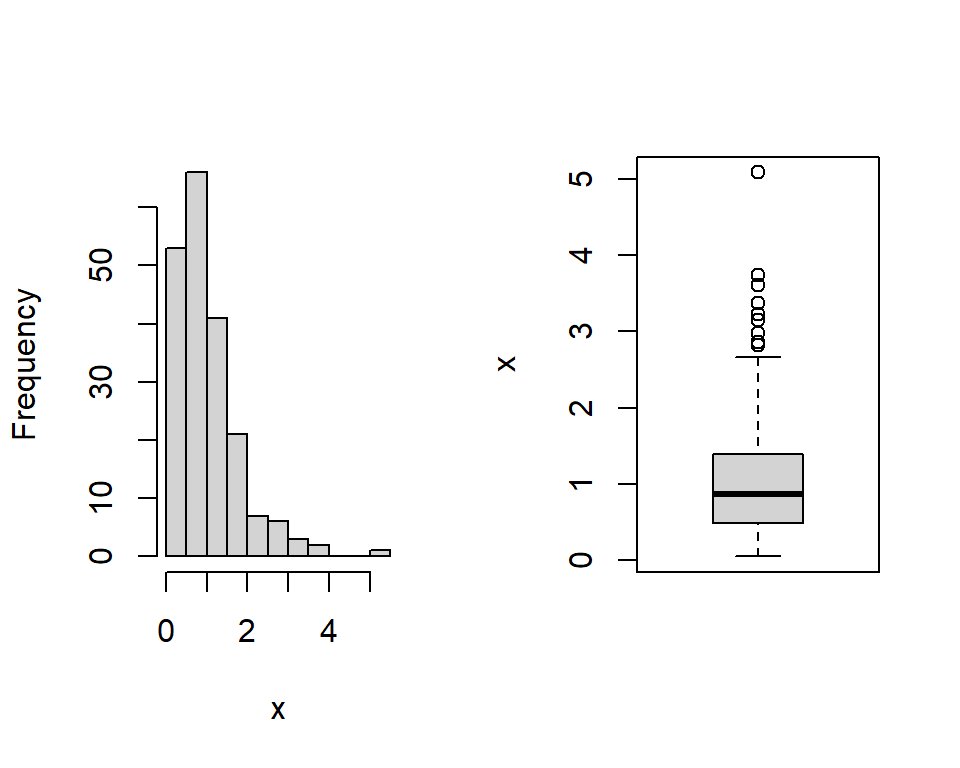
\includegraphics{IntroStats_files/figure-latex/unnamed-chunk-17-1} \end{center}

\textbf{Q3.7} The methods useful for assessing the relationship between pairs of variables depends on the type of data. In the examples below, there are a mix of quantitative and qualitative variables.

\textbf{Q3.7} \textbf{a.} Ethnicity and type of employment (e.g.~retail, agricultural, medical). Both variables are qualitative and so a frequency table showing the numbers in each category would be created. From the frequency table, the percentages in each category can be obtained.

\textbf{Q3.7} \textbf{b.} Volume of rainfall (litres) and the amount of runoff on an airport runway (litres). Both these variables are continuous and so a scatterplot would illustrate the relationship between them.

\textbf{Q3.7} \textbf{c.} Temperature (\(^o\)C) and habitat type (e.g.~Farmland, woodland). Temperature is a continuous variable and habitat type is qualitative and so side-by-side boxplots, or a series of histograms (one histogram of temperature for each habitat type), could be used to display the relationship.

\hypertarget{part-probability-and-distributions}{%
\part{Probability and Distributions}\label{part-probability-and-distributions}}

\hypertarget{probability}{%
\chapter{Probability}\label{probability}}

\hypertarget{INTprob}{%
\section{Introduction}\label{INTprob}}

{ \emph{Probability: as a measurable quantity: the extent to which a particular event is likely to occur, or a particular situation be the case, as measured by the relative frequency of occurrence of events of the same kind in the whole course of experience, and expressed by a number between 0 and 1.}
Oxford English Dictionary \citeyearpar{dictionary1989oxford}}

Here we define probability, consider how to represent it mathematically, present some axioms and basic results, and work through some example probability calculations. By the end of the this chapter, you should be able to

\begin{enumerate}
\def\labelenumi{\arabic{enumi}.}
\tightlist
\item
  distinguish the different definitions of probability
\item
  understand the basic axioms of probability.
\item
  understand Bayes' theorem and its simple applications
\end{enumerate}

In 2006, the polling organisation, Populus Limited, randomly sampled 1,509 adults, age 18 and older, by telephone between January 6\(^{th}\) and 8\(^{th}\) and asked each adult their voting intention (Labour, Conservative, Liberal Democrat, and Other). The resulting percentages were:

\label{tab:Votint} Voting intention in Populus survey.

\begin{table}
\label{Votint}
\caption{Voting Intention in Populus survey}
\end{table}

\begin{longtable}[]{@{}ll@{}}
\toprule
Party & Percentage\tabularnewline
\midrule
\endhead
Labour & 39\tabularnewline
Conservative & 36\tabularnewline
Liberal Democrat & 16\tabularnewline
Other & 9\tabularnewline
\bottomrule
\end{longtable}

How close are these sample \textbf{statistics} to the population \textbf{parameters}? A different sample would have got a different answer , so there must be uncertainty associated with these sample statistics.

Sampled value = Parameter + Chance Error

i.e.~signal + noise

The parameter(s) in this case are the unknown population proportions.

\begin{itemize}
\tightlist
\item
  So what is the magnitude of the error?
\item
  Ideas from probability will help with this.
\end{itemize}

Througout statistics, we consider the evaluation of hypotheses where we attach a probability to a particular event given a particular set of results. This allows us to decide whether to accept or reject the hypotheses. Therefore, this chapter will consider the concept of probability in some detail.

\hypertarget{random-phenomena-and-uncertain-outcomes}{%
\subsection{Random phenomena and uncertain outcomes}\label{random-phenomena-and-uncertain-outcomes}}

Lots of processes present us with uncertainty - consider processes that are random, repeatable and uncertain.

\textbf{For example}

\begin{itemize}
\tightlist
\item
  Process: Toss a coin

  \begin{itemize}
  \tightlist
  \item
    Outcomes: Head, Tail, Side
  \end{itemize}
\item
  Process: A person who does not have HIV is tested for HIV

  \begin{itemize}
  \tightlist
  \item
    Outcomes: Negative test result, Positive test result (a false positive)
  \end{itemize}
\item
  Process: Departure time of a flight from Edinburgh to London on an airline.

  \begin{itemize}
  \tightlist
  \item
    Outcomes: the flight departs on time, 1 minute late, 2 minutes late, etc
  \end{itemize}
\end{itemize}

Probability is a branch of mathematics that deals with the quantification of uncertainty.

A few things to remember about probabilities:

\begin{itemize}
\tightlist
\item
  Probabilities must lie between 0 and 1 (and cannot be larger than one or less than zero)
\item
  Probabilities are sometimes expressed as percentages, e.g.~0 = 0\%, 0.2 = 20\%, 0.02 = 2\%
\end{itemize}

\hypertarget{sample-spaces-and-events}{%
\section{Sample spaces and events}\label{sample-spaces-and-events}}

There are a lot of terms (explained below) related to the possible outcomes of a random process:

\begin{itemize}
\tightlist
\item
  sample space,
\item
  elementary events,
\item
  compound events,
\item
  mutually exclusive events,
\item
  independent events.
\end{itemize}

1. The collection of all possible outcomes of an experiment is the \textbf{sample space}, and is denoted \(\mathcal{S}\) (or as in Figure \ref{fig:Vennunion}. \(\Omega\)). Examples of sample spaces:

\begin{itemize}
\tightlist
\item
  Toss Coin: \(\mathcal{S}\) = \{H,T\} (Note the use of curly brackets to indicate a set.). We will assume from here on, that the chance of a coin falling on its side is so negligible that it can be ignored.
\item
  HIV Test: \(\mathcal{S}\) = \{Negative, Positive\}
\item
  Airplane actual departure time - scheduled departure time: \(\mathcal{S}\) = \{0 to 360 minutes\} assuming the flight is cancelled after 3 hours.
\end{itemize}

2. A subset of outcomes in \(\mathcal{S}\) is called an Event and it's often labelled by a capital letter, e.g.~\(A\).

Let \(A\) and \(B\) be any two events defined on a particular sample space.

For example The set of all possible outcomes occurring: \(A\) alone, \(B\) alone, or in either \(A\) and \(B\)..

\begin{itemize}
\tightlist
\item
  union of \(A\) and \(B\), \(A \cup B\) or \(A ~\mbox{or}~ B\) (Figure \ref{fig:Vennunion}).
\end{itemize}

\begin{figure}

{\centering 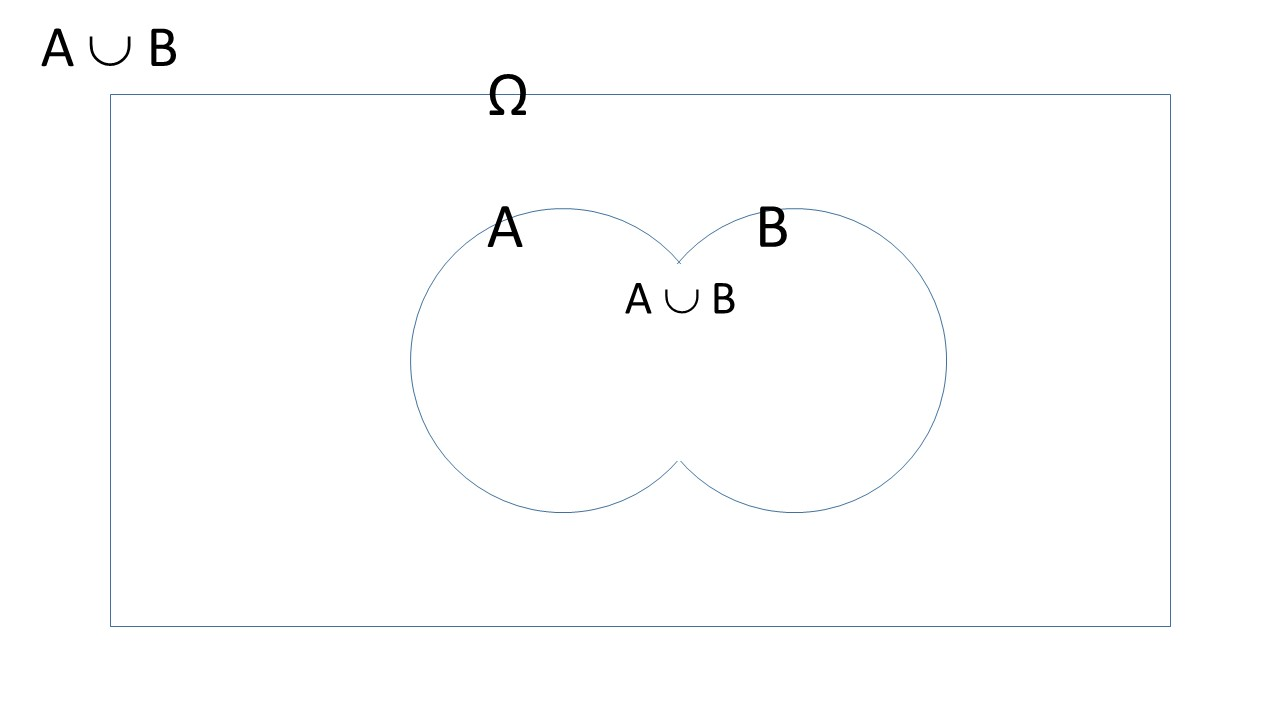
\includegraphics[width=1\linewidth]{./figures/AunionB} 

}

\caption{A Venn diagram of the union of events A and B}\label{fig:Vennunion}
\end{figure}

\begin{itemize}
\item
  The set of all events in \(\mathcal{S}\) that do not occur in A is: complement of \(A\) or \(\overline{A}\) or \(A^c\).
\item
  When \(A\) and \(B\) have no outcomes in common, they are mutually exclusive or disjoint, i.e., \(A \cap B\) = \(\emptyset\). \(\emptyset\) means empty set.
\end{itemize}

If there is just one outcome in an event A, the event is called simple or elementary, otherwise it is called compound.

When \(A\) and \(B\) have no outcomes in common, they are \textbf{mutually exclusive} or \textbf{disjoint}, i.e., \(A \cap B\) = \(\emptyset\)

The set of all outcomes occurring only in both \(A\) and \(B\) is

\begin{itemize}
\tightlist
\item
  intersection of \(A\) and \(B\), \(A \cap B\), or \(A ~\mbox{and}~ B\) (Figure \ref{fig:Vennintercept}).
\end{itemize}

\begin{figure}

{\centering 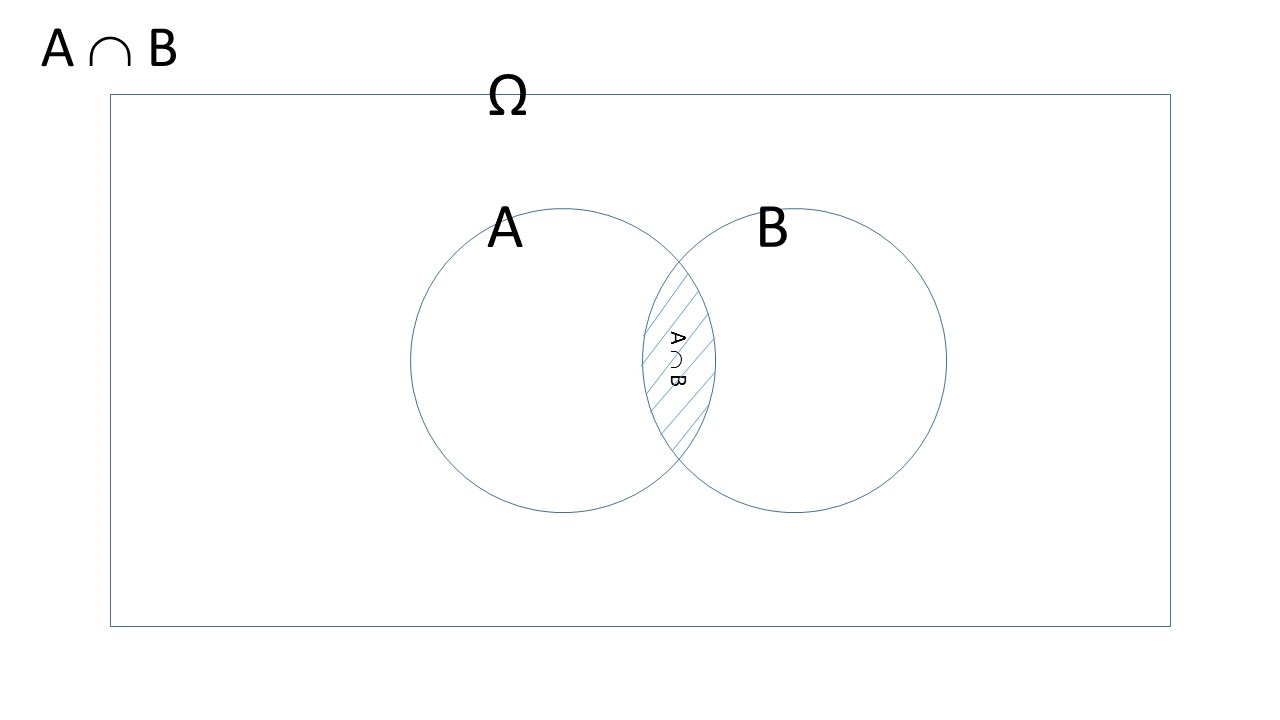
\includegraphics[width=1\linewidth]{./figures/AinterceptB} 

}

\caption{A Venn diagram of the intercept of events A and B}\label{fig:Vennintercept}
\end{figure}

\begin{itemize}
\tightlist
\item
  The set of all events in S that do not occur in \(A\) is the \textbf{complement} of \(A\) or \(\overline{A}\) or \(A^c\). So if the probability of sighting the Loch Ness Monster in a day at Loch Ness is 0.3 (e.g.~\(Pr(Nessie)=0.3\)) then the probability we don't see anything would be \(Pr(\overline{Nessie})=1-0.3=0.7\).
  This is called the \textbf{law of complementary probability}.
\end{itemize}

\textbf{Example} Roll 2 dice and count the total number of dots face up. Define the two events \(A\) and \(B\) as follows:

\(A\) = get an even number
\(B\) = get a number that is divisible by 3

Thus \(A\) = (\{2\}, \{4\}, \{6\}, \{8\}, \{10\}, \{12\}). and \(B\) = (\{3\}, \{6\}, \{9\}, \{12\}). Then

\begin{itemize}
\tightlist
\item
  \(A \cup B\) = \{2,3,4,6,8,9,10,12\}
\item
  \(A \cap B\) = \{6,12\}
\item
  \(A^c\) = \{3,5,7,9,11\}
\item
  Are \(A\) and \(B\) disjoint? No.~\(A \cap B \ne \emptyset\).
\end{itemize}

This example contain \emph{stochasticity} - a particular realisation of the process isn't completely predictable. The usual way of treating this is probabilistically.

\hypertarget{definition-of-probability-and-3-axioms}{%
\section{Definition of Probability and 3 Axioms}\label{definition-of-probability-and-3-axioms}}

\hypertarget{probability-1}{%
\subsection{Probability}\label{probability-1}}

Informally: Consider a process, with multiple uncertain outcomes, that could be repeated infinitely often, in an identical and independent fashion, then the probability of an event \(A\), \(\Pr(A)\), is the long run relative frequency of \(A\).

How does the above definition compare to probability in the following contexts?

\begin{itemize}
\tightlist
\item
  \textbf{Q4.1} The probability I win on a European roulette wheel choosing 1 number?
\item
  \textbf{Q4.2} The probability that I win any money on a spin of an mechanical one-armed bandit?
\item
  \textbf{Q4.3} The probability that the All Blacks win the 2019 world cup?
\item
  \textbf{Q4.4} The probability of rain tomorrow in St Andrews 10-11am is 0.07 (7\% chance)?
\item
  \textbf{Q4.5} The probability of nuclear war breaking out tomorrow?
\end{itemize}

\hypertarget{three-axioms}{%
\subsection{Three Axioms}\label{three-axioms}}

Formally probability can be described by 3 axioms.

\begin{itemize}
\item
  (Axiom 1) The probability of an event \(A \in S\), denoted \(\Pr(A)\) is a number between 0 and 1, inclusive.
\item
  (Axiom 2) \(\Pr(S)\) = 1
\item
  (Axiom 3) If \(A_1\), \(A_2\), \(\ldots\), \(A_k\) are a finite collection of mutually exclusive events, then
\end{itemize}

\[
\Pr(A_1 \cup A_2 \cup \ldots \cup A_k)  =  \sum_{i=1}^k \Pr(A_i)
\]

Informally, this is called the Addition Rule. Applies if \(k\) is infinite too.

These mean practically:

\begin{itemize}
\tightlist
\item
  Things that never happen get probability value 0.
\item
  Things that are certain get probability value 1.
\item
  Uncertain things get quantified between 0 and 1.
\item
  We need to know all possible outcomes to assign probabilities.
\item
  You can add probabilities of mutually exclusive things to get the probability one of them happens.
\end{itemize}

\emph{Example} The outcomes of a single die roll are 1, 2, 3, 4, 5, 6. The probabiity of getting any number at all is one from the second axion. What is the probability of getting an even number?

\[
\begin{aligned}
         \Pr(2 \cup 4 \cup 6) &= \Pr(2) + \Pr(4) + \Pr(6)\\ 
         &= \frac{1}{6} + \frac{1}{6} + \frac{1}{6} = \frac{1}{2} = 0.5 
\end{aligned}
\]

This uses Axiom 3 since \(2\), \(4\), and \(6\) are mutually exclusive.

\hypertarget{three-results-of-the-axioms}{%
\subsection{Three results of the Axioms}\label{three-results-of-the-axioms}}

All the other rules of probability come from these axioms

\begin{itemize}
\item
  Complement rule: \(\Pr(A^c) = 1 - \Pr(A)\).
\item
  General addition rule.
\end{itemize}

\(\Pr(A \cup B) = \Pr(A) + \Pr(B) - \Pr(A \cap B)\).

We have to remove \(\Pr(A \cap B)\) otherwise we would be counting that event space twice. Therefore, we adjust the sum of the two probabilities by subtracting the probability of the two events occurring together.This is called the \textbf{general addition rule}.

\begin{itemize}
\item
  Intersection of 2 mutually exclusive events:

  \begin{itemize}
  \tightlist
  \item
    If \(A\) and \(B\) are \textbf{mutually exclusive}, then \(\Pr(A \cap B) = 0\).(i.e.~they cannot occur together and the addition formula reduces to:
  \end{itemize}
\end{itemize}

\[Pr(A \cup B) = Pr(A) + Pr(B)\]

Remember to think of \(\cap\) as \textbf{AND} and \(\cup\) as \textbf{OR}

\hypertarget{independence-and-the-multiplication-rule}{%
\section{Independence and the Multiplication Rule}\label{independence-and-the-multiplication-rule}}

Formally, if two events \(A\) and \(B\) are independent, then

\[\Pr(A ~and~ B) = \Pr(A) \times \Pr(B)\]

Thus when two events are independent, the probability of \textbf{both} happening is the product of the two individual probabilities.

In plain language this means the occurrence of one event does not affect the probability of the other occurring.

Independence makes probability calculations easy - it is often assumed (but often not true)

\hypertarget{testing-for-independence}{%
\subsection{Testing for Independence}\label{testing-for-independence}}

We can assess if events F and G are actually independent using the multiplication rule where we ask if \(Pr(A) \times Pr(B)=Pr(A \cap B)\)

\emph{Example} A fair coin will be tossed twice. Let \(A\) be the event of
a Head on the first toss and \(B\) be the event of a Tail on the second toss.

The outcomes for two different flips should be independent (since the coin has no memory).

Thus, \(\Pr(A ~and~ B)\) = \(\Pr(A) \times \Pr(B)\) = 0.5 \(\times\) 0.5 = 0.25.

This could be tested by tossing the coin numerous times and seeing if the long run frequency matched 0.25.

\textbf{Q4.6.} In an ordinary card deck there are 52 cards: 4 suits (diamonds, hearts,
clubs, spades) of 13 cards (Ace,2,3,\(\ldots\),10,J,Q,K). A deck is shuffled
and one card is drawn and removed, and a second card is drawn. Let \(A\) = first
card = 2 of Spades and \(B\)=second card is 3 of spades. What is \(\Pr(A ~and~ B)\)?

\hypertarget{conditional-probabilities}{%
\section{Conditional probabilities}\label{conditional-probabilities}}

If there is partial information about the result of a random process, that
information can be used to calculate conditional probabilities for particular events. Conditional probabilities are often the most interesting (and counter intuitive!) aspects of probability-based work.

\begin{itemize}
\item
  Consider two events \(S\) and \(D\)

  \begin{itemize}
  \tightlist
  \item
    \(S\) = the event that one or more animals were seen in a sampling location and
  \item
    \(D\) = a randomly chosen sampling location was in a desert.
  \end{itemize}
\item
  We are now interested in the probability of \(S\) occurring \textbf{given} that \(D\) has occurred. What is the probability of seeing an animal if you are are looking in a desert. This probability is written as \(Pr (S|D)\), and is called the \textbf{conditional probability} of \(S\) given \(D\):
\end{itemize}

\[Pr(S|D) = \frac{Pr(S \cap D)}{Pr(D)}\]

If \(S\) and \(D\) are \textbf{independent} then whether \(D\) occurred or not will not affect \(Pr(S)\), so that \(Pr(S|D) = Pr(S)\).

\begin{itemize}
\item
  Consider two events A and B

  \begin{itemize}
  \tightlist
  \item
    A = the event that a head is tossed
  \item
    B = the event that a tail is tossed
  \end{itemize}

  In this case coin tosses are independent
\end{itemize}

Substituting this into the rule of conditional probability gives
\[Pr(A|B) = Pr(A) = \frac{Pr(A \cap B)} {Pr(B)}\]
and rearranging gives you the \textbf{multiplication rule} (see above).

\[ Pr(A) \times Pr(B) = Pr(A \cap B) \]

Explanation by example. This example is taken from Moore \citeyearpar{Moore1992}.

\begin{itemize}
\tightlist
\item
  A cross tabulation of suicides classified by victim and whether or not a firearm was used:
\end{itemize}

\begin{longtable}[]{@{}llll@{}}
\toprule
& Male & Female & Total\tabularnewline
\midrule
\endhead
Firearm & 16,381 & 2,559 & 18,940\tabularnewline
Other & 9,034 & 3,536 & 12,570\tabularnewline
Total & 25,415 & 6,095 & 31,510\tabularnewline
\bottomrule
\end{longtable}

\begin{itemize}
\tightlist
\item
  We convert the table into a relative frequency table with 4 categories by dividing throughout by the grand total 31,510, e.g.~the total proportion of males is \(25415/31510 = 0.807\):
\end{itemize}

\begin{longtable}[]{@{}llll@{}}
\toprule
& Male & Female & Total\tabularnewline
\midrule
\endhead
Firearm & 0.520 & 0.081 & 0.601\tabularnewline
Other & 0.287 & 0.112 & 0.399\tabularnewline
Total & 0.807 & 0.193 & 1.000\tabularnewline
\bottomrule
\end{longtable}

Let \(G\) be the event that a firearm was used then \(\Pr(G)\) = 0.601. If \(F\) be the event that a victim is female then \(\Pr(F)\) = 0.193.

\begin{itemize}
\tightlist
\item
  If you know the victim was Female (i.e.~\textbf{Given} Female), what is the probability a firearm was used? We need the values from the table that represent the probability that the victim was Female \textbf{and} used a firearm (0.081) and the probability the victim was Female (0.193):
\end{itemize}

\[Pr(G|F) = \frac{Pr(G \cap F)} {Pr(F)} = \frac{0.081}{0.193} = 0.420\]

\begin{itemize}
\tightlist
\item
  Therefore the probability of a firearm being used \textbf{given} it was a women
  is an example of \textbf{conditional probability}.
\end{itemize}

\hypertarget{independence-revisited}{%
\subsection{Independence revisited}\label{independence-revisited}}

One definition of independence is that two events \(A\) and \(B\) are independent when \(\Pr(A|B)\)=\(\Pr(A)\), or equivalently \(\Pr(B|A)\)=\(\Pr(B)\).

In words, knowing that \(B\) occurred tells one nothing about the probability of \(A\). The general multiplication rule reduces to ``the'\,' multiplication rule:

\[
    \Pr(A ~and~ B)  =  \Pr(A|B) \times \Pr(B) = \Pr(A) \times \Pr(B) 
\]

\hypertarget{tree-diagrams}{%
\section{Tree Diagrams}\label{tree-diagrams}}

A sometimes useful technique for calculating probabilities when there is a sequence
of random processes is to draw a tree diagram.

``\emph{A tree diagram is a device used to enumerate all possible outcomes of a sequence of procedures, where the number of possible outcomes for each procedure is finite}''
(paraphrasing Lipshutz \citeyearpar{Lipshutz2011}).

This approach can be used as a simple way of considering problems that might involve complex probabilities.

\textbf{Example} Let us suppose that the probability a woman age 40 has breast cancer is 1\%. If she has breast cancer the probability she tests positive on a screening mammogram is 99 \%. If she does not have breast cancer the probability that she nonetheless tests positive is 9\%.

What are the chances that a woman who tests positive actually has breast cancer?

Considered as a conditional probability problem it is complex.
We know:
\(Pr(Cancer)\) = 0.01
\(Pr(positive|Cancer)\) = 0.99
\(Pr(positive|Not cancer)\) = 0.09

So the question is what is Pr(Cancer\textbar positive)?

This can be calculated as

\begin{eqnarray*}
 \Pr(Cancer|positive)  =  \frac{\Pr(Cancer \cap positive)}{\Pr(positive)}
\end{eqnarray*}

But it is not immediately obvious what \(\Pr(Cancer \cap positive)\) and \(\Pr(positive)\) actually are.

Considering this as a tree diagram things (Figure \ref{fig:tree1}) become a little more obvious.

\begin{figure}

{\centering 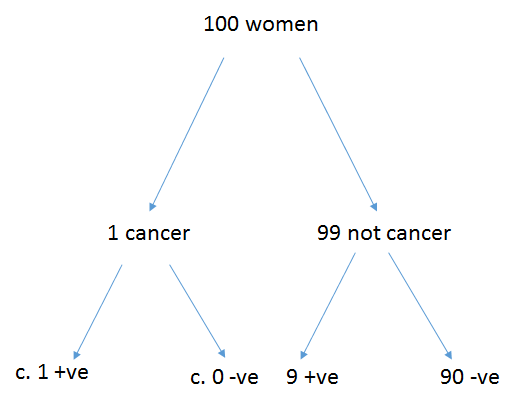
\includegraphics[width=0.95\linewidth]{figures/treediagram} 

}

\caption{All possible outcomes for 100 women.}\label{fig:tree1}
\end{figure}

Of 100 women, 1 has cancer and tests positive, 99 do not have cancer of whom
9/100 x 99 = 8.9 will test positive.

It now becomes easy to see that the \(Pr(Cancer|positive)\) = 1/(1+8.9) = 10.1\%

See Gigerenzer \citeyearpar{Gigerenzer2003} for more on this.

\textbf{Example} (adapted from Lipshutz \& Lipson 2011): ``Dragos and Christopher play a tennis tournament. The first person to win 2 games in a row or who wins a total of three games wins the tournament.'' On average Dragos has a 0.6 probability of winning an individual match and Christopher a 0.4 probability of winning an individual match. What is the probability Dragos wins the tournament.

We can tackle something simple like this by complete enumeration of outcomes. The following concepts are needed: independence (winning a game does not alter the chance of a future win of a game) and mutual exclusivity (only one player can win a match).

\begin{figure}

{\centering 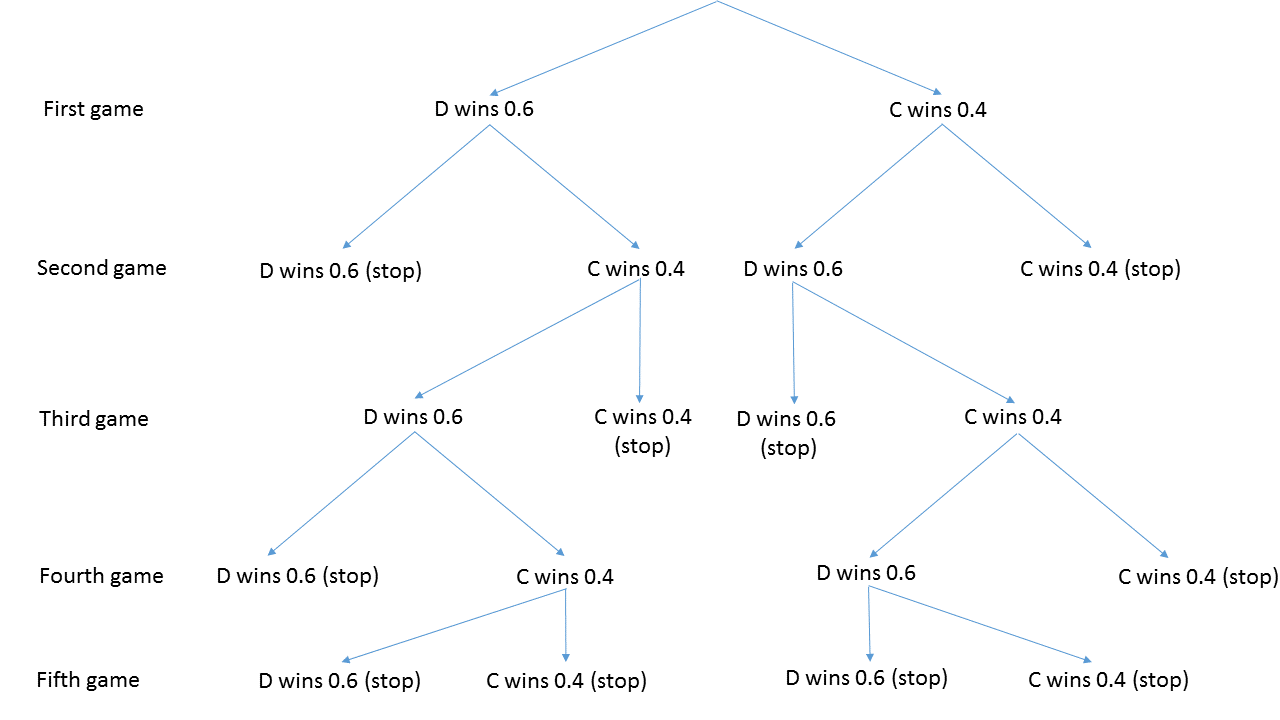
\includegraphics[width=0.95\linewidth]{figures/treediagramdrago} 

}

\caption{Tree for match outcomes.}\label{fig:tree2}
\end{figure}

The probablity of Dragos winning is
\[0.6 \times 0.6 + 0.6 \times 0.4 \times 0.6 \times 0.6 + 0.6 \times 0.4 \times 0.6 \times 0.4 \times 0.6 + 0.4 \times 0.6 \times 0.6 +0.4 \times 0.6 \times 0.4 \times 0.6 \times 0.6\]
\[= 0.360 + 0.086 + 0.035 + 0.144 +0.035 = 0.660\]

Some lessons arising for later:\\
How would I establish the baseline probabilities of each player winning a match?\\
In \emph{reality}, what confidence is associated with my assessment? What influences this?

\hypertarget{marginal-and-joint-probabilities}{%
\section{Marginal and joint probabilities}\label{marginal-and-joint-probabilities}}

When considering data that can be classified in a variety of ways it is often useful to consider the probabilities that can be generated from such data. When considering just one factor then the probabilities are \textbf{marginal} (for reasons that will become clear in a moment). If two or more factors are considered then the derived probabilites are \textbf{joint}.

For example, passengers of the Titanic can be viewed in terms of two ``random'\,' processes, living or dying after the ship hit the iceberg, and what class ticket they purchased.

\begin{itemize}
\tightlist
\item
  There were 2,201 people on the Titanic and the numbers cross-classified by two categories are:
\end{itemize}

\begin{longtable}[]{@{}llllll@{}}
\toprule
Fate & First & Second & Third & Crew & Total\tabularnewline
\midrule
\endhead
Lived & 203 & 118 & 178 & 212 & 711\tabularnewline
Died & 122 & 167 & 528 & 673 & 1490\tabularnewline
Total & 325 & 285 & 706 & 885 & 2201\tabularnewline
\bottomrule
\end{longtable}

Dividing the cell values, and row and column totals, by the grand total
yields a matrix of `'probabilities''.

\begin{longtable}[]{@{}llllll@{}}
\toprule
Fate & First & Second & Third & Crew & Total\tabularnewline
\midrule
\endhead
Lived & 0.092 & 0.054 & 0.081 & 0.096 & 0.323\tabularnewline
Died & 0.056 & 0.076 & 0.240 & 0.306 & 0.677\tabularnewline
Total & 0.148 & 0.129 & 0.321 & 0.402 & 1.000\tabularnewline
\bottomrule
\end{longtable}

For example, \(\Pr(Live \cap Second)\)=0.054, a joint probability, the proportion of the total of people on board the Titanic who were second class passengers and survived.
And \(\Pr(Live)\)=0.323, a marginal probability, the total proportion of people on board who lived. It is marginal because it is calculated from the margins of the table.

Of further interest are particular conditional probabilities, such as
did the ticket class have an effect on the probability of living?
These are conditional probabilities.

\begin{itemize}
\tightlist
\item
  For example, \textbf{given} that one had a First class ticket, what was the probability of surviving?
\end{itemize}

Substituting this into the rule of conditional probability gives
\[Pr(Lived|First)  = \frac{Pr(Lived \cap First)} {Pr(First)} = \frac{0.092} {0.148} = 0.622\]

\begin{itemize}
\tightlist
\item
  So \(Pr(Lived|First)\) is conditional.
\item
  \(Pr(Lived \cap First)\) is joint.
\item
  \(Pr(First)\) is marginal.
\end{itemize}

\hypertarget{SUMprob}{%
\section{Summary}\label{SUMprob}}

Understanding the basics of probability is extremely useful in interpreting evidence and in applying the tests and models that come later in the module.\\
If you want to learn more about the philisophical aspects of probability then consider taking the module \emph{Statistical Thinking}.

\hypertarget{learning-objectives-1}{%
\subsection{Learning objectives}\label{learning-objectives-1}}

By the end of the this unit, you should be able to

\begin{enumerate}
\def\labelenumi{\arabic{enumi}.}
\tightlist
\item
  distinguish the different definitions of probability
\item
  understand the basic axioms of probability.
\item
  understand Bayes' theorem and its simple applications
\end{enumerate}

\hypertarget{ANSprob}{%
\section{Answers}\label{ANSprob}}

\textbf{Q4.1} A European roulette wheel has 37 slots. So the chance of winning on a single number is 1/37. This could be determined as a long run frequency.

\textbf{Q4.2} To determine the exact probability one would need to know the number of wheels, the numerical breakdown of images on each wheel and knowledge of which combinations of images earn a payout. A more practical statistic is the expected return per pound for example. Understandably fruit machine producers are reluctant to supply this information unless compelled by law. This could be determined from a long run frequency.

\textbf{Q4.3} We can never know precisely the probability of a sports team winning a cup as there are so many variables. We might use historical sports statistics to generate a probability based on the performance of similar teams in the past. It would be difficult to determine this as a long run frequency as no teams will remain constant.

\textbf{Q4.4}The probability of rain tomorrow could be estimated by a mechanistic physical model which considers the weather conditions based on physical principles. Alternatively the probability of rain could be estimated statistically based on past similar weather conditions. Hence a long run frequency could be considered.

\textbf{Q4.5} Here it is rather difficult to predict the probabilities from observed events. The given probability comes from belief.

\textbf{Q4.6} \(Pr(A \cup B) = Pr(A) + Pr(B)\) but event B can only be regarded as independent if Pr(B) is adjusted for the fact that drawing the first card has altered things. There are \(4 \times 13 =52\) card
The probability of obtaining the first card is 1/52. The probability of obtaining the second card is 1/51 because before the second draw there are only 51 cards in the back.
So \(Pr(A \cap B) = Pr(A) \times Pr(B) = 1/52 \times 1/51 = 1/2652\).

\hypertarget{discreterv}{%
\chapter{Discrete random variables}\label{discreterv}}

\emph{{[}Professor Moriarty{]} is a man of good birth and excellent education, endowed by nature with a phenomenal mathematical faculty. At the age of twenty-one, he wrote a treatise upon the binomial theorem, which has had a European vogue. On the strength of it he won the mathematical chair at one of our smaller universities, and had, to all appearances, a most brilliant career before him.} Sir Arthur Conan Doyle \citeyearpar{Doyle1894}

\hypertarget{INTdiscrv}{%
\section{Introduction}\label{INTdiscrv}}

A \textbf{random variable} is a quantity that can take a range of values that cannot be predicted with certainty but only described probabilistically (\citet{BorowskiBorwein}). The values can either be discrete or continuous. In this unit, discrete random values are considered; continuous random values are considered in the following chapter.

In this unit, we define:

\begin{itemize}
\item
  discrete random variables,
\item
  probability mass functions,
\item
  cumulative distribution functions
\item
  expected values and expected variation of discrete random variables,
\item
  and three specific and useful random variables, Bernoulli, binomial and Poisson random variables.
\end{itemize}

Note that this chapter contains a lot of notation and many equations; please refer to the notation guide.

\hypertarget{discrete-random-variables}{%
\section{Discrete random variables}\label{discrete-random-variables}}

A discrete random variable is random variable which can only take a countable number of values.

As an example, consider tossing a fair coin twice; the possible outcomes are head-head, head-tail, tail-head and tail-tail. Assume that the variable of interest is the number of heads (denoted by \(Y\)) and so the resulting values, or sample space, for \(Y\) are either 0, 1 or 2 heads (Table \ref{tab:coinoutcometab}).

\begin{longtable}[]{@{}ccccc@{}}
\caption{\label{tab:coinoutcometab} The possible outcomes (H=head, T=tail) for tossing a coin twice and the resulting combinations of heads (\(Y\)).}\tabularnewline
\toprule
\endhead
\begin{minipage}[t]{(\columnwidth - 4\tabcolsep) * \real{0.19}}\centering
\textbf{Outcome}\strut
\end{minipage} & \begin{minipage}[t]{(\columnwidth - 4\tabcolsep) * \real{0.07}}\centering
HH\strut
\end{minipage} & \begin{minipage}[t]{(\columnwidth - 4\tabcolsep) * \real{0.07}}\centering
HT\strut
\end{minipage} & \begin{minipage}[t]{(\columnwidth - 4\tabcolsep) * \real{0.07}}\centering
TH\strut
\end{minipage} & \begin{minipage}[t]{(\columnwidth - 4\tabcolsep) * \real{0.07}}\centering
TT\strut
\end{minipage}\tabularnewline
\begin{minipage}[t]{(\columnwidth - 4\tabcolsep) * \real{0.19}}\centering
\textbf{Y}\strut
\end{minipage} & \begin{minipage}[t]{(\columnwidth - 4\tabcolsep) * \real{0.07}}\centering
2\strut
\end{minipage} & \begin{minipage}[t]{(\columnwidth - 4\tabcolsep) * \real{0.07}}\centering
1\strut
\end{minipage} & \begin{minipage}[t]{(\columnwidth - 4\tabcolsep) * \real{0.07}}\centering
1\strut
\end{minipage} & \begin{minipage}[t]{(\columnwidth - 4\tabcolsep) * \real{0.07}}\centering
0\strut
\end{minipage}\tabularnewline
\bottomrule
\end{longtable}

The variable \(Y\) is a discrete random variable; the outcome can only be a discrete value and we cannot predict the outcome with certainty but we can describe the outcome probabilistically.

\hypertarget{probability-mass-function}{%
\subsection{Probability mass function}\label{probability-mass-function}}

The probability mass function (PMF) is simply a mathematical description of the probabilities of outcomes in the sample space. We can construct the PMF for \(Y\), the number of heads when tossing a coin twice by considering the possible outcomes (Table \ref{tab:coinoutcometab}). The sample space is either no heads, one head or two heads (i.e.~\(S\)=\{0, 1, 2\}). The probability of two heads, written \(Pr(Y=2)\), will be 1 out of 4 possible outcomes, thus \(Pr(Y=2)=0.25\). Similar calculations can be used to obtain the probability of no heads and one head (Table \ref{tab:pmfex1tab}).

\begin{longtable}[]{@{}cccc@{}}
\caption{\label{tab:pmfex1tab} Probability mass function for \(Y\), the number of heads when a coin is tossed twice.}\tabularnewline
\toprule
\endhead
\begin{minipage}[t]{(\columnwidth - 3\tabcolsep) * \real{0.19}}\centering
\textbf{y}\strut
\end{minipage} & \begin{minipage}[t]{(\columnwidth - 3\tabcolsep) * \real{0.10}}\centering
0\strut
\end{minipage} & \begin{minipage}[t]{(\columnwidth - 3\tabcolsep) * \real{0.08}}\centering
1\strut
\end{minipage} & \begin{minipage}[t]{(\columnwidth - 3\tabcolsep) * \real{0.10}}\centering
2\strut
\end{minipage}\tabularnewline
\begin{minipage}[t]{(\columnwidth - 3\tabcolsep) * \real{0.19}}\centering
\textbf{Pr(Y=y)}\strut
\end{minipage} & \begin{minipage}[t]{(\columnwidth - 3\tabcolsep) * \real{0.10}}\centering
0.25\strut
\end{minipage} & \begin{minipage}[t]{(\columnwidth - 3\tabcolsep) * \real{0.08}}\centering
0.5\strut
\end{minipage} & \begin{minipage}[t]{(\columnwidth - 3\tabcolsep) * \real{0.10}}\centering
0.25\strut
\end{minipage}\tabularnewline
\bottomrule
\end{longtable}

The PMF tells us everything about the random variable \(Y\). It also has a special property in that if we sum \(Pr(Y=y)\) over all possible values in the sample space, we get 1.

If the sample space of a random variable denoted by \(X\) can be written as \{\({k, k+1, ... , n}\)\} then

\begin{align}
\sum_{x=k}^{n} Pr(X=x) = Pr(X=k) + Pr(X=k+1) + ... + Pr(X=n) = 1
\end{align}

This property is easy to verify for the PMF of \(Y\), the number of heads:

\[\sum_{y=0}^{2} Pr(Y=y) = Pr(Y=0) + Pr(Y=1) + Pr(Y=2) = 0.25 + 0.5 + 0.25 = 1\]

\textbf{Q5.1} Let event \(Y\) be the sum of the numbers resulting from throwing two fair, six-sided die. Calculate the probability mass function of \(Y\).

\hypertarget{cumulative-distribution-function}{%
\subsection{Cumulative distribution function}\label{cumulative-distribution-function}}

The cumulative distribution function (CDF) is derived from the PMF. For a discrete random variable called \(X\), the CDF provides the probability that \(Pr(X \le x)\). Thus, for the coin tossing example, the probability that \(Y\) is less than or equal to one head (i.e.~\(Pr(Y \le 1)\)) is given by:

\[Pr(Y \le 1) = Pr(Y=0) + Pr(Y=1) = 0.25 + 0.5 = 0.75\]
A similar calculation can be performed for all values in the sample space (Table \ref{tab:cdfex1tab}).

\begin{longtable}[]{@{}cccc@{}}
\caption{\label{tab:cdfex1tab} Probability mass function (\(Pr(Y=y)\)) and cumulative distribution function (\(Pr(Y \le y)\)) for \(Y\), the number of heads when a coin is tossed twice.}\tabularnewline
\toprule
\endhead
\begin{minipage}[t]{(\columnwidth - 3\tabcolsep) * \real{0.21}}\centering
\textbf{y}\strut
\end{minipage} & \begin{minipage}[t]{(\columnwidth - 3\tabcolsep) * \real{0.10}}\centering
0\strut
\end{minipage} & \begin{minipage}[t]{(\columnwidth - 3\tabcolsep) * \real{0.10}}\centering
1\strut
\end{minipage} & \begin{minipage}[t]{(\columnwidth - 3\tabcolsep) * \real{0.10}}\centering
2\strut
\end{minipage}\tabularnewline
\begin{minipage}[t]{(\columnwidth - 3\tabcolsep) * \real{0.21}}\centering
\textbf{Pr(Y=y)}\strut
\end{minipage} & \begin{minipage}[t]{(\columnwidth - 3\tabcolsep) * \real{0.10}}\centering
0.25\strut
\end{minipage} & \begin{minipage}[t]{(\columnwidth - 3\tabcolsep) * \real{0.10}}\centering
0.5\strut
\end{minipage} & \begin{minipage}[t]{(\columnwidth - 3\tabcolsep) * \real{0.10}}\centering
0.25\strut
\end{minipage}\tabularnewline
\begin{minipage}[t]{(\columnwidth - 3\tabcolsep) * \real{0.21}}\centering
\textbf{Pr(Y\textless=y)}\strut
\end{minipage} & \begin{minipage}[t]{(\columnwidth - 3\tabcolsep) * \real{0.10}}\centering
0.25\strut
\end{minipage} & \begin{minipage}[t]{(\columnwidth - 3\tabcolsep) * \real{0.10}}\centering
0.75\strut
\end{minipage} & \begin{minipage}[t]{(\columnwidth - 3\tabcolsep) * \real{0.10}}\centering
1\strut
\end{minipage}\tabularnewline
\bottomrule
\end{longtable}

The CDF is a useful tool in calculating probabilities over intervals of a discrete random variable. However, care must be taken in considering the endpoints of the intervals - are they inclusive or exclusive; this will be clearer with a more complicated example.

Consider the toss of a fair, six-sided die and denote it by \(X\); there are six possible outcomes (i.e.~1 to 6), all with equal probability (Table \ref{tab:cdfex2tab}). We can obtain the probability that \(X\) is less than 5 from the CDF as follows:

\[Pr(X < 5) = Pr(X \le 4) = 0.6667\]

\begin{longtable}[]{@{}ccccccc@{}}
\caption{\label{tab:cdfex2tab} PMF and CDF of \(X\), the toss of six-sided die.}\tabularnewline
\toprule
\endhead
\begin{minipage}[t]{(\columnwidth - 6\tabcolsep) * \real{0.21}}\centering
\textbf{x}\strut
\end{minipage} & \begin{minipage}[t]{(\columnwidth - 6\tabcolsep) * \real{0.12}}\centering
1\strut
\end{minipage} & \begin{minipage}[t]{(\columnwidth - 6\tabcolsep) * \real{0.12}}\centering
2\strut
\end{minipage} & \begin{minipage}[t]{(\columnwidth - 6\tabcolsep) * \real{0.12}}\centering
3\strut
\end{minipage} & \begin{minipage}[t]{(\columnwidth - 6\tabcolsep) * \real{0.12}}\centering
4\strut
\end{minipage} & \begin{minipage}[t]{(\columnwidth - 6\tabcolsep) * \real{0.12}}\centering
5\strut
\end{minipage} & \begin{minipage}[t]{(\columnwidth - 6\tabcolsep) * \real{0.12}}\centering
6\strut
\end{minipage}\tabularnewline
\begin{minipage}[t]{(\columnwidth - 6\tabcolsep) * \real{0.21}}\centering
\textbf{Pr(X=x)}\strut
\end{minipage} & \begin{minipage}[t]{(\columnwidth - 6\tabcolsep) * \real{0.12}}\centering
0.1667\strut
\end{minipage} & \begin{minipage}[t]{(\columnwidth - 6\tabcolsep) * \real{0.12}}\centering
0.1667\strut
\end{minipage} & \begin{minipage}[t]{(\columnwidth - 6\tabcolsep) * \real{0.12}}\centering
0.1667\strut
\end{minipage} & \begin{minipage}[t]{(\columnwidth - 6\tabcolsep) * \real{0.12}}\centering
0.1667\strut
\end{minipage} & \begin{minipage}[t]{(\columnwidth - 6\tabcolsep) * \real{0.12}}\centering
0.1667\strut
\end{minipage} & \begin{minipage}[t]{(\columnwidth - 6\tabcolsep) * \real{0.12}}\centering
0.1667\strut
\end{minipage}\tabularnewline
\begin{minipage}[t]{(\columnwidth - 6\tabcolsep) * \real{0.21}}\centering
\textbf{Pr(X\textless=x)}\strut
\end{minipage} & \begin{minipage}[t]{(\columnwidth - 6\tabcolsep) * \real{0.12}}\centering
0.1667\strut
\end{minipage} & \begin{minipage}[t]{(\columnwidth - 6\tabcolsep) * \real{0.12}}\centering
0.3333\strut
\end{minipage} & \begin{minipage}[t]{(\columnwidth - 6\tabcolsep) * \real{0.12}}\centering
0.5\strut
\end{minipage} & \begin{minipage}[t]{(\columnwidth - 6\tabcolsep) * \real{0.12}}\centering
0.6667\strut
\end{minipage} & \begin{minipage}[t]{(\columnwidth - 6\tabcolsep) * \real{0.12}}\centering
0.8333\strut
\end{minipage} & \begin{minipage}[t]{(\columnwidth - 6\tabcolsep) * \real{0.12}}\centering
1\strut
\end{minipage}\tabularnewline
\bottomrule
\end{longtable}

What happens if we want \(Pr(X>x)\) or \(Pr(X \ge x)\)? These can be found using the complement rule (Chapter \ref{probability}):

\[Pr(X>x) = 1-Pr(X \leq x)\]
\[Pr(X\ge x) = 1-Pr(X < x) = 1 - Pr(X \le (x-1))\]
Hence, the probability that \(X > 4\) can be found from
\[Pr(X > 4) = 1 - Pr(X \le 4) = 1 - 0.6667 = 0.333\]

\[Pr(X \ge 4) = 1 - Pr(X < 4) = 1 - Pr(X \le 3) = 1 - 0.5 = 0.5\]

With discrete random variables, it is important to be careful with \(<\), \(\le\), \(>\) and \(\ge\) signs.

\textbf{Q5.2} Using the PMF obtained for event \(Y\) defined in Q5.1,

\textbf{a.} Calculate the cumulative distribution function of \(Y\).

\textbf{b.} What is the probability that \(Y\) will be less than 7?

\textbf{c.} What is the probability that \(Y\) will be an odd number?

\textbf{d.} Include question to calculate an interval estimate.

\hypertarget{expectation}{%
\subsection{Expectation}\label{expectation}}

Although the outcome of a process is uncertain, the PMF can be used to determine what value might be expected on average, if the process was to be repeated many times. For a discrete random variable \(X\), with a finite number of outcomes \(k\), the \textbf{expected value} of \(X\), denoted by \(E(X)\) is given by

\begin{align}
E(X) = \sum_{x=k}^n xPr(X=x)
\end{align}

This is actually a weighted average where the probabilities are the weights (since the probabilities sum to one).

Using this equation, the expected value from tossing a die is therefore given by

\[E(X) = (1 \times 0.1667) + (2 \times 0.1667) + (3 \times 0.1667) + (4 \times 0.1667) + (5 \times 0.1667) + (6 \times 0.1667) = 3.5\]

The same calculation can be seen in Table \ref{tab:pmfex2tab}.

\begin{longtable}[]{@{}cccccccc@{}}
\caption{\label{tab:pmfex2tab} Calculations to obtain the expected value.}\tabularnewline
\toprule
\endhead
\begin{minipage}[t]{(\columnwidth - 7\tabcolsep) * \real{0.18}}\centering
\textbf{x}\strut
\end{minipage} & \begin{minipage}[t]{(\columnwidth - 7\tabcolsep) * \real{0.12}}\centering
1\strut
\end{minipage} & \begin{minipage}[t]{(\columnwidth - 7\tabcolsep) * \real{0.12}}\centering
2\strut
\end{minipage} & \begin{minipage}[t]{(\columnwidth - 7\tabcolsep) * \real{0.12}}\centering
3\strut
\end{minipage} & \begin{minipage}[t]{(\columnwidth - 7\tabcolsep) * \real{0.12}}\centering
4\strut
\end{minipage} & \begin{minipage}[t]{(\columnwidth - 7\tabcolsep) * \real{0.12}}\centering
5\strut
\end{minipage} & \begin{minipage}[t]{(\columnwidth - 7\tabcolsep) * \real{0.12}}\centering
6\strut
\end{minipage} & \begin{minipage}[t]{(\columnwidth - 7\tabcolsep) * \real{0.12}}\centering
Total\strut
\end{minipage}\tabularnewline
\begin{minipage}[t]{(\columnwidth - 7\tabcolsep) * \real{0.18}}\centering
\textbf{Pr(X=x)}\strut
\end{minipage} & \begin{minipage}[t]{(\columnwidth - 7\tabcolsep) * \real{0.12}}\centering
0.16667\strut
\end{minipage} & \begin{minipage}[t]{(\columnwidth - 7\tabcolsep) * \real{0.12}}\centering
0.16667\strut
\end{minipage} & \begin{minipage}[t]{(\columnwidth - 7\tabcolsep) * \real{0.12}}\centering
0.16667\strut
\end{minipage} & \begin{minipage}[t]{(\columnwidth - 7\tabcolsep) * \real{0.12}}\centering
0.16667\strut
\end{minipage} & \begin{minipage}[t]{(\columnwidth - 7\tabcolsep) * \real{0.12}}\centering
0.16667\strut
\end{minipage} & \begin{minipage}[t]{(\columnwidth - 7\tabcolsep) * \real{0.12}}\centering
0.16667\strut
\end{minipage} & \begin{minipage}[t]{(\columnwidth - 7\tabcolsep) * \real{0.12}}\centering
1\strut
\end{minipage}\tabularnewline
\begin{minipage}[t]{(\columnwidth - 7\tabcolsep) * \real{0.18}}\centering
\textbf{xPr(X=x)}\strut
\end{minipage} & \begin{minipage}[t]{(\columnwidth - 7\tabcolsep) * \real{0.12}}\centering
0.16667\strut
\end{minipage} & \begin{minipage}[t]{(\columnwidth - 7\tabcolsep) * \real{0.12}}\centering
0.33333\strut
\end{minipage} & \begin{minipage}[t]{(\columnwidth - 7\tabcolsep) * \real{0.12}}\centering
0.50000\strut
\end{minipage} & \begin{minipage}[t]{(\columnwidth - 7\tabcolsep) * \real{0.12}}\centering
0.66667\strut
\end{minipage} & \begin{minipage}[t]{(\columnwidth - 7\tabcolsep) * \real{0.12}}\centering
0.83333\strut
\end{minipage} & \begin{minipage}[t]{(\columnwidth - 7\tabcolsep) * \real{0.12}}\centering
1.00000\strut
\end{minipage} & \begin{minipage}[t]{(\columnwidth - 7\tabcolsep) * \real{0.12}}\centering
3.5\strut
\end{minipage}\tabularnewline
\bottomrule
\end{longtable}

The expected value from tossing a six-sided die is 3.5, i.e.~\(E(X)=3.5\). We could verify this empirically if we were to throw the die a large number of times and compute the average value of all the observed outcomes. As the number of throws increases, the average will converge to 3.5 - the simple arithmetic mean of all outcomes. Hence, if all outcomes are equally likely, as in the case of a fair die, then the expected value is simply the arithmetic mean, in the long term. If the probabilities are not equal, the expected value takes into account that all outcomes are not equally likely and a weighted average must be used.

\textbf{Q5.3} What is the expected value for event \(Y\) defined in Q5.1.

\hypertarget{variance}{%
\subsection{Variance}\label{variance}}

Since we cannot say with certainty what the outcome of an event will be, but only what is likely, or expected, there will be some uncertainty associated with the expected value. Can we commonly expect values to be close to the mean value or far from the mean value?

To quantify the degree to which the values differ from the expected value, or how spread out they may be, we calculate the variance of \(X\), denoted by \(Var(X)\):

\begin{align}
Var(X) = \sum_{x=k}^n (x - E(X))^2Pr(X=x)
\end{align}

Thus, the variance for the outcome of tossing a die is given by:

\[Var(X)= (1-3.5)^2 \times 0.1667 + (2-3.5)^2 \times 0.1667 + (3-3.5)^2 \times 0.1667 + (4-3.5)^2 \times 0.1667 + (5-3.5)^2 \times 0.1667 + (6-3.5)^2 \times 0.1667\]
\[= 1.04167 + 0.37500 + 0.04167 + 0.04167 + 0.3750 + 1.04167 = 2.917 \]

Again, we can add columns in the PMF table to help with this calculation (Table \ref{tab:pmfex3tab}).

\begin{longtable}[]{@{}ccccc@{}}
\caption{\label{tab:pmfex3tab} Intermediate calculations to obtain the variance for a fair, six sided die. (continued below)}\tabularnewline
\toprule
\endhead
\begin{minipage}[t]{(\columnwidth - 4\tabcolsep) * \real{0.39}}\centering
\textbf{\(x\)}\strut
\end{minipage} & \begin{minipage}[t]{(\columnwidth - 4\tabcolsep) * \real{0.15}}\centering
1\strut
\end{minipage} & \begin{minipage}[t]{(\columnwidth - 4\tabcolsep) * \real{0.15}}\centering
2\strut
\end{minipage} & \begin{minipage}[t]{(\columnwidth - 4\tabcolsep) * \real{0.15}}\centering
3\strut
\end{minipage} & \begin{minipage}[t]{(\columnwidth - 4\tabcolsep) * \real{0.15}}\centering
4\strut
\end{minipage}\tabularnewline
\begin{minipage}[t]{(\columnwidth - 4\tabcolsep) * \real{0.39}}\centering
\textbf{\(x-E(X)\)}\strut
\end{minipage} & \begin{minipage}[t]{(\columnwidth - 4\tabcolsep) * \real{0.15}}\centering
-2.5\strut
\end{minipage} & \begin{minipage}[t]{(\columnwidth - 4\tabcolsep) * \real{0.15}}\centering
-1.5\strut
\end{minipage} & \begin{minipage}[t]{(\columnwidth - 4\tabcolsep) * \real{0.15}}\centering
-0.5\strut
\end{minipage} & \begin{minipage}[t]{(\columnwidth - 4\tabcolsep) * \real{0.15}}\centering
0.5\strut
\end{minipage}\tabularnewline
\begin{minipage}[t]{(\columnwidth - 4\tabcolsep) * \real{0.39}}\centering
\textbf{\((x-E(X))^2\)}\strut
\end{minipage} & \begin{minipage}[t]{(\columnwidth - 4\tabcolsep) * \real{0.15}}\centering
6.25\strut
\end{minipage} & \begin{minipage}[t]{(\columnwidth - 4\tabcolsep) * \real{0.15}}\centering
2.25\strut
\end{minipage} & \begin{minipage}[t]{(\columnwidth - 4\tabcolsep) * \real{0.15}}\centering
0.25\strut
\end{minipage} & \begin{minipage}[t]{(\columnwidth - 4\tabcolsep) * \real{0.15}}\centering
0.25\strut
\end{minipage}\tabularnewline
\begin{minipage}[t]{(\columnwidth - 4\tabcolsep) * \real{0.39}}\centering
\textbf{\((x-E(X))^2\)Pr\((X=x)\)}\strut
\end{minipage} & \begin{minipage}[t]{(\columnwidth - 4\tabcolsep) * \real{0.15}}\centering
1.041667\strut
\end{minipage} & \begin{minipage}[t]{(\columnwidth - 4\tabcolsep) * \real{0.15}}\centering
0.375000\strut
\end{minipage} & \begin{minipage}[t]{(\columnwidth - 4\tabcolsep) * \real{0.15}}\centering
0.041667\strut
\end{minipage} & \begin{minipage}[t]{(\columnwidth - 4\tabcolsep) * \real{0.15}}\centering
0.041667\strut
\end{minipage}\tabularnewline
\bottomrule
\end{longtable}

\begin{longtable}[]{@{}cccc@{}}
\toprule
\endhead
\begin{minipage}[t]{(\columnwidth - 3\tabcolsep) * \real{0.39}}\centering
\textbf{\(x\)}\strut
\end{minipage} & \begin{minipage}[t]{(\columnwidth - 3\tabcolsep) * \real{0.15}}\centering
5\strut
\end{minipage} & \begin{minipage}[t]{(\columnwidth - 3\tabcolsep) * \real{0.15}}\centering
6\strut
\end{minipage} & \begin{minipage}[t]{(\columnwidth - 3\tabcolsep) * \real{0.11}}\centering
Total\strut
\end{minipage}\tabularnewline
\begin{minipage}[t]{(\columnwidth - 3\tabcolsep) * \real{0.39}}\centering
\textbf{\(x-E(X)\)}\strut
\end{minipage} & \begin{minipage}[t]{(\columnwidth - 3\tabcolsep) * \real{0.15}}\centering
1.5\strut
\end{minipage} & \begin{minipage}[t]{(\columnwidth - 3\tabcolsep) * \real{0.15}}\centering
2.5\strut
\end{minipage} & \begin{minipage}[t]{(\columnwidth - 3\tabcolsep) * \real{0.11}}\centering
\strut
\end{minipage}\tabularnewline
\begin{minipage}[t]{(\columnwidth - 3\tabcolsep) * \real{0.39}}\centering
\textbf{\((x-E(X))^2\)}\strut
\end{minipage} & \begin{minipage}[t]{(\columnwidth - 3\tabcolsep) * \real{0.15}}\centering
2.25\strut
\end{minipage} & \begin{minipage}[t]{(\columnwidth - 3\tabcolsep) * \real{0.15}}\centering
6.25\strut
\end{minipage} & \begin{minipage}[t]{(\columnwidth - 3\tabcolsep) * \real{0.11}}\centering
\strut
\end{minipage}\tabularnewline
\begin{minipage}[t]{(\columnwidth - 3\tabcolsep) * \real{0.39}}\centering
\textbf{\((x-E(X))^2\)Pr\((X=x)\)}\strut
\end{minipage} & \begin{minipage}[t]{(\columnwidth - 3\tabcolsep) * \real{0.15}}\centering
0.375000\strut
\end{minipage} & \begin{minipage}[t]{(\columnwidth - 3\tabcolsep) * \real{0.15}}\centering
1.041667\strut
\end{minipage} & \begin{minipage}[t]{(\columnwidth - 3\tabcolsep) * \real{0.11}}\centering
2.917\strut
\end{minipage}\tabularnewline
\bottomrule
\end{longtable}

The square root of the variance of \(X\) is equal to the standard deviation of \(X\),

\begin{align}
sd(X) = \sqrt {Var(X)}
\end{align}

Therefore, for tossing a six-sided die, the standard deviation will be:

\[sd(X) = \sqrt{Var(X)} = \sqrt{2.917} = 1.708\]

\textbf{Q5.4} What is the variance and standard deviation value for event \(Y\) defined in Q5.1.

\hypertarget{special-discrete-distributions}{%
\section{Special discrete distributions}\label{special-discrete-distributions}}

There are several discrete random variables and associated distributions which are frequently used in statistics; here we describe the Bernoulli, binomial and Poisson distributions.

\hypertarget{bernoulli-distribution}{%
\subsection{Bernoulli distribution}\label{bernoulli-distribution}}

A Bernoulli random variable is a discrete random variable which can only have two possible outcomes (e.g.~success/failure, yes/no, heads/tails) and these outcomes are represented by 0 and 1. The probability distribution takes the value of 1 with probability \(p\) and the value \(0\) with probability \(q=1-p\).

For example, in a single coin toss (denoted by \(X\)) we could represent a head with a 1 and a tail with 0 (or vice versa). The probability of obtaining a head, \(Pr(X=1) = 0.5\) and so the probability of obtaining a tail is \(Pr(X=0) = 1 - 0.5=0.5\). The PMF is shown in Table \ref{tab:pmffaircoin}.

\begin{longtable}[]{@{}lll@{}}
\caption{\label{tab:pmffaircoin} The PMF for tossing a fair coin; Head=1 and Tail=0.}\tabularnewline
\toprule
\(x\) & 1 & 0\tabularnewline
\midrule
\endfirsthead
\toprule
\(x\) & 1 & 0\tabularnewline
\midrule
\endhead
\(Pr(X=x)\) & \(p\) = 0.5 & \(1-p\) = 0.5\tabularnewline
& &\tabularnewline
\bottomrule
\end{longtable}

\textbf{Q5.5} Using the information in Table \ref{tab:pmffaircoin}, calculate the expected value of a fair coin?

\textbf{Q5.6} When practising darts, a darts player considers hitting a bull's eye with a dart as a success and considers missing the bull's eye as a failure. The probability they manage to hit a bull's eye is 0.25. Create and complete a PMF for the throw of a single dart.

\hypertarget{binomial-distribution}{%
\subsection{Binomial distribution}\label{binomial-distribution}}

Let \(Y_1\), \(Y_2\), \ldots, \(Y_n\) be \(n\) independent, Bernoulli random variables with the \textbf{same} probability of success, \(p\). Independence means that the outcome from one event has no effect on subsequent events. Define a new variable that is the sum:

\[X = \sum_{i=1}^n Y_i\]
\(X\) is called a \textbf{binomial} random variable and is described by two parameters, the number of trials \(n\) and the probability of success, \(p\). This is written concisely using the notation \(X \sim \textrm{Binomial}(n, p)\). The random variable \(X\) is the total number of successes out of \(n\) trials and follows a binomial distribution provided that:

\begin{enumerate}
\def\labelenumi{\arabic{enumi}.}
\tightlist
\item
  there are only two possible outcomes for each individual trial,
\item
  the probability of success, \(p\), is constant for all trials,
\item
  there are a fixed number of trials, \(n\), and
\item
  each trial is independent of other trials.
\end{enumerate}

For \(x\) in the set \{0, 1, \ldots, \(n\)\}, the probability mass function of the \(\textrm{Binomial}(n, p)\) distribution will provide the probability of obtaining \(x\) successes out of \(n\) trials:

\begin{align}
Pr(X=x) = \frac{n!}{x!(n-x)!}p^x (1-p)^{(n-x)}
\end{align}

As an example, consider a game of darts; assume the probability of hitting the bull's-eye is 0.25 and that one throw has no effect on subsequent throws (i.e.~each throw is independent). What is the probability of hitting the bull's-eye exactly once in 4 attempts? Let \(X\) denote hitting a bull's-eye (a success); we have four attempts (or trials) and so \(n=4\), the probability of a success for each attempt is \(p=0.25\). We want the probability of exactly one success, so \(x=1\). Thus, using equation 5:

\[Pr(X=1) = \frac{4!}{1!(4-1)!}(0.25)^1 (1-0.25)^{(4-1)} = \frac{4!}{1!3!} \times 0.25 \times (0.75)^3\]

\[ = 4 \times 0.25 \times 0.421875 = 0.4218\]

We can think of this equation in a more intuitive way and consider each of the components. There are four ways of throwing exactly one bull's eye in four attempts - we could hit the bull's eye on the first, second, third or fourth attempt. The probability of throwing one bull's eye is 0.25 and the probability of missing on three attempts is given by \(0.75 \times 0.75 \times 0.75\). Thus, putting all the components together, we have \(4 \times 0.25 \times (0.75)^3 = 0.4218\) which is what we had previously. It does not matter that the bull's eye was the first, second, third or fourth attempt - the binomial distribution does not consider the order of events.

Equation 5 can be used to complete the PMF for this example (i.e.~obtain the probability for 0, 1, 2, 3 and 4 bull's eye in four attempts). However, as we have seen doing these calculations can be a bit long-winded. Fortunately, there is an R function to do this.

\hypertarget{binomR}{%
\subsubsection{Doing this in R}\label{binomR}}

To calculate values from a binomial distribution, there are a special group of functions with the suffix, \texttt{binom}. To obtain a probability (i.e.~\(Pr(X=x)\)) we use the \texttt{dbinom} function and need to specify the parameters of the binomial distribution (i.e.~\(n\) and \(p\)).

\begin{Shaded}
\begin{Highlighting}[]
\CommentTok{\# Calculate the probability from a binomial distribution}
\NormalTok{n }\OtherTok{\textless{}{-}} \DecValTok{4} \CommentTok{\# number of trials}
\NormalTok{xsuccess }\OtherTok{\textless{}{-}} \DecValTok{1} \CommentTok{\# required number of successes}
\NormalTok{p }\OtherTok{\textless{}{-}} \FloatTok{0.25} \CommentTok{\# probability of a success}
\FunctionTok{dbinom}\NormalTok{(}\AttributeTok{x=}\NormalTok{xsuccess, }\AttributeTok{size=}\NormalTok{n, }\AttributeTok{prob=}\NormalTok{p)}
\end{Highlighting}
\end{Shaded}

\begin{verbatim}
[1] 0.421875
\end{verbatim}

The \texttt{dbinom} function can be used to calculate the probabilities associated with all possible outcomes and thus create the PMF. The possible outcomes range from no bull's eyes in four throws up to four bull's eyes.

\begin{Shaded}
\begin{Highlighting}[]
\CommentTok{\# Create the PMF }
\NormalTok{results }\OtherTok{\textless{}{-}} \FunctionTok{data.frame}\NormalTok{(}\AttributeTok{x=}\DecValTok{0}\SpecialCharTok{:}\DecValTok{4}\NormalTok{) }\CommentTok{\# Specify all possible outcomes}
\CommentTok{\# Check dataframe has been created correctly}
\NormalTok{results}
\end{Highlighting}
\end{Shaded}

\begin{verbatim}
  x
1 0
2 1
3 2
4 3
5 4
\end{verbatim}

\begin{Shaded}
\begin{Highlighting}[]
\CommentTok{\# Calculate the probabilty of each outcome}
\NormalTok{results}\SpecialCharTok{$}\NormalTok{PMF }\OtherTok{\textless{}{-}} \FunctionTok{dbinom}\NormalTok{(}\AttributeTok{x=}\NormalTok{results}\SpecialCharTok{$}\NormalTok{x, }\AttributeTok{size=}\NormalTok{n, }\AttributeTok{prob=}\NormalTok{p)}
\NormalTok{results}
\end{Highlighting}
\end{Shaded}

\begin{verbatim}
  x        PMF
1 0 0.31640625
2 1 0.42187500
3 2 0.21093750
4 3 0.04687500
5 4 0.00390625
\end{verbatim}

Another function, \texttt{pbinom}, calculates the CDF as follows:

\begin{Shaded}
\begin{Highlighting}[]
\CommentTok{\# Calculate the CDF}
\NormalTok{results}\SpecialCharTok{$}\NormalTok{CDF }\OtherTok{\textless{}{-}} \FunctionTok{pbinom}\NormalTok{(}\AttributeTok{q=}\NormalTok{results}\SpecialCharTok{$}\NormalTok{x, }\AttributeTok{size=}\NormalTok{n, }\AttributeTok{prob=}\NormalTok{p)}
\NormalTok{results}
\end{Highlighting}
\end{Shaded}

\begin{verbatim}
  x        PMF       CDF
1 0 0.31640625 0.3164063
2 1 0.42187500 0.7382812
3 2 0.21093750 0.9492188
4 3 0.04687500 0.9960938
5 4 0.00390625 1.0000000
\end{verbatim}

\hypertarget{visualising-the-binomial-distribution-for-different-values-of-n-and-p}{%
\subsubsection{\texorpdfstring{Visualising the binomial distribution for different values of \(n\) and \(p\)}{Visualising the binomial distribution for different values of n and p}}\label{visualising-the-binomial-distribution-for-different-values-of-n-and-p}}

We can think about the change in the shape of the binomial distribution as the probability of success changes, for example, Figure \ref{fig:binomfreq} shows the PMF for \(n\)=10 and three different values of \(p\):

\begin{itemize}
\item
  when \(p\) is low (e.g.~\(p=0.1\)) we only expect to see a small number of successes out of the 10 trials and the distribution is skewed to the right - we can't have fewer than zero successes and we don't see many high values.
\item
  when \(p\) is 0.5 we may expect to see about half of the 10 trials are successful and the distribution is symmetrical - about half the time we see more than 5 successes and about half the time we see fewer than 5 successes (out of the 10 trials).
\item
  when \(p\) is high (e.g.~\(p=0.9\)), we expect a large number of successes out of the 10 trials and the distribution is skewed to the left - we can't have more than ten successes and we don't see many low values.
\end{itemize}

\begin{figure}

{\centering 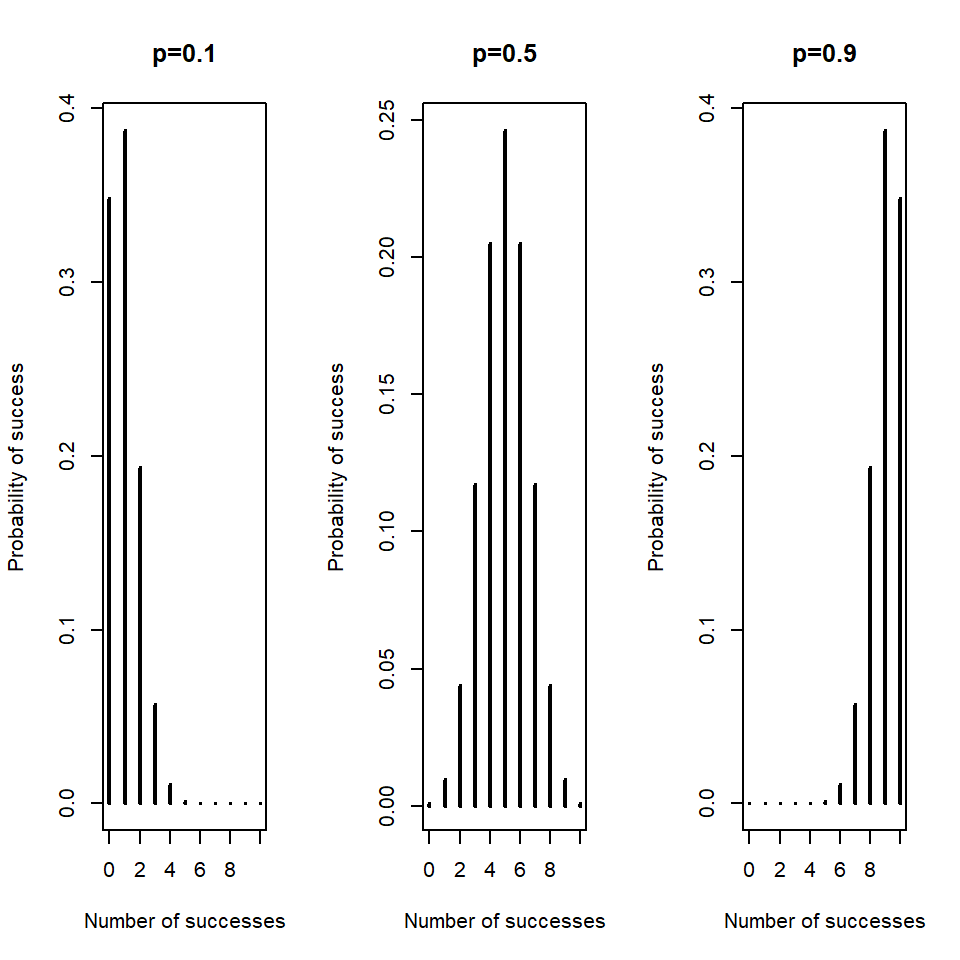
\includegraphics[width=.8\linewidth]{IntroStats_files/figure-latex/binomfreq-1} 

}

\caption{Probability mass functions for three different probabilities, $p$, and 10 trials.}\label{fig:binomfreq}
\end{figure}

You can explore some other combinations of \(p\) and \(n\) in Figure \ref{fig:binshiny}. There is also a live version \href{https://moniquemackenzie.shinyapps.io/IntroStats_Binomial/}{here}



\begin{figure}

{\centering \href{https://moniquemackenzie.shinyapps.io/IntroStats_Binomial/}{\includegraphics{IntroStats_files/figure-latex/binshiny-1} }

}

\caption{Visualising the Binomial distribution. You can see a live version by clicking \href{https://moniquemackenzie.shinyapps.io/IntroStats_Binomial/}{here}}\label{fig:binshiny}
\end{figure}

\hypertarget{expectation-and-variance}{%
\subsubsection{Expectation and variance}\label{expectation-and-variance}}

Using equation 5, we can calculate the probability the darts player throws none, one, two, three or four bull's eyes but what is the number of bull's eyes that the darts player might expect to hit in the long term, given they have four attempts? For a binomial random variable, there is a simple formula to calculate the expected number.

The expected value of a binomial random variable is given by

\begin{align}
E(X) = np
\end{align}

and the variance is found from

\begin{align}
Var(X) = np(1-p)
\end{align}

Thus, the number of times the darts player would expect to hit the bull's eye with 4 throws is

\[E(X) = 4 \times 0.25 = 1\]

and the variance is

\[Var(X) = 4 \times 0.25 \times (1-0.25) = 0.75\]

\textbf{Q5.7} In an online quiz, there are 10 multiple-choice questions and 4 possible options for each question, with only one correct option per question. A student, who is short on time, decides to randomly select an option for each question.

\textbf{a.} What is the probability of selecting the correct option for a question?

\textbf{b.} What is the expected number of questions that the student will answer correctly?

\textbf{c.} What is the probability of answering all questions correctly?

\textbf{d.} What is the probability of answering no questions correctly?

\textbf{e.} Is the student more likely to select the correct answer for every question or the wrong answer for every question?

\textbf{Q5.8} Use the PMF values shown in section \ref{binomR} for throwing four darts (i.e.~the output from R) and equation 2 to confirm that the expected number of bull's eye the player could be expected to throw is 1. Use equation 3 to confirm that the variance is 0.75 and hence calculate the standard deviation.

\hypertarget{poisdist}{%
\subsection{Poisson distribution}\label{poisdist}}

The Poisson distribution is used to describe the number of events occurring in some time interval, if these events occur at a known constant mean rate (\(\lambda\)) and independently of the time since the last event. An example of a Poisson variable might be the number of cars passing a certain point within a ten minute period. The interval could also apply to a specified area or volume, for example, the number of trees in a hectare.

A Poisson random variable \(X\) is a discrete random variable with an infinite, but countable, set of possible values, in particular \(X\) can equal values 0, 1, 2, 3, \ldots, and \(\lambda > 0\). This can be written as \(X \sim \textrm{Poisson}(\lambda)\).

The PMF for a Poisson random variable \(X\) is given by

\[ Pr(X=x) = \frac{e^{-\lambda}\lambda^x}{x!}\]
For example, the probability that \(X=3\) given that events occur with a mean rate \(\lambda=4\) is found from:

\[ Pr(X=3) = \frac{e^{-4} \times 4 \times 3}{3!} = \frac{1.1722}{6} = 0.1954\]

The underlying process that gives rise to a Poisson distribution is one where:

\begin{itemize}
\tightlist
\item
  \(x\) is the number of times that an event occurs in some interval and \(x\) can take values 0, 1, 2, \ldots{}
\item
  events are independent, i.e.~the occurrence of one event does not affect the occurrence of a second event
\item
  the mean rate of occurrence, \(\lambda\), is independent of occurrences. This is usually assumed to be constant but in reality may vary over time.
\item
  two events cannot occur at exactly the same instant, instead at each very small sub-interval either exactly one event occurs or does not occur.
\end{itemize}

Consider the following example; \textit{Xeroderma pigmentosum} (XP) is a genetic disorder which means that affected individuals are extremely sensitive to ultraviolet rays. The frequency in the U.S. and Europe is approximately 1 person in 250,000 people. If 1,000,000 people are randomly sampled, what is the probability that five people with XP are selected?

The mean rate of XP occurrence in one million people, \(\lambda\), is 4 people per million and we want the probability of selecting 5 people with XP from a million. Hence,

\[Pr(X=5) = \frac{e^{-4}4^5}{5!} = \frac{18.755}{120} = 0.156\]

\hypertarget{doing-this-in-r-5}{%
\subsubsection{Doing this in R}\label{doing-this-in-r-5}}

Similar to the binomial distribution, there are a suite of functions that can be used to obtain values from a Poisson distribution - the suffix is \texttt{pois}.

Using the example above, the probability of selecting 5 people with XP given \(\lambda=4\) can be found using:

\begin{Shaded}
\begin{Highlighting}[]
\FunctionTok{dpois}\NormalTok{(}\AttributeTok{x=}\DecValTok{5}\NormalTok{, }\AttributeTok{lambda=}\DecValTok{4}\NormalTok{)}
\end{Highlighting}
\end{Shaded}

\begin{verbatim}
[1] 0.1562935
\end{verbatim}

The CDF is found using the \texttt{ppois} function. For example this function can be used to calculate the probability of selecting less than 3 people with XP (i.e.~\(Pr(X \le 3)\)).

\begin{Shaded}
\begin{Highlighting}[]
\CommentTok{\# CDF }
\FunctionTok{ppois}\NormalTok{(}\AttributeTok{q=}\DecValTok{3}\NormalTok{, }\AttributeTok{lambda=}\DecValTok{4}\NormalTok{)}
\end{Highlighting}
\end{Shaded}

\begin{verbatim}
[1] 0.4334701
\end{verbatim}

\begin{Shaded}
\begin{Highlighting}[]
\CommentTok{\# This is equivalent to}
\FunctionTok{dpois}\NormalTok{(}\AttributeTok{x=}\DecValTok{0}\NormalTok{, }\AttributeTok{lambda=}\DecValTok{4}\NormalTok{) }\SpecialCharTok{+} \FunctionTok{dpois}\NormalTok{(}\AttributeTok{x=}\DecValTok{1}\NormalTok{, }\AttributeTok{lambda=}\DecValTok{4}\NormalTok{) }\SpecialCharTok{+} \FunctionTok{dpois}\NormalTok{(}\AttributeTok{x=}\DecValTok{2}\NormalTok{, }\AttributeTok{lambda=}\DecValTok{4}\NormalTok{) }\SpecialCharTok{+} \FunctionTok{dpois}\NormalTok{(}\AttributeTok{x=}\DecValTok{3}\NormalTok{, }\AttributeTok{lambda=}\DecValTok{4}\NormalTok{) }
\end{Highlighting}
\end{Shaded}

\begin{verbatim}
[1] 0.4334701
\end{verbatim}

\hypertarget{expected-value-and-variance}{%
\subsubsection{Expected value and variance}\label{expected-value-and-variance}}

A Poisson random variable has the interesting property such that the expected value and the variance are equal to the mean rate of occurrence:

\[E(X) = Var(X) = \lambda\]
Thus, returning to the example of the genetic disorder, the expected number of people out of one million people with XP is 4 and the variance is 4.

The standard deviation is given by

\[sd(X) = \sqrt{\lambda}\]

\textbf{Q5.9} The number of people buying an umbrella per day from a shop in April is Poisson
distributed with mean rate 4.5. What is the probability that at least 3 people buy an umbrella on an April day? Confirm your calculation using R.

\hypertarget{comparison-of-binomial-and-poisson-distributions}{%
\subsection{Comparison of binomial and Poisson distributions?}\label{comparison-of-binomial-and-poisson-distributions}}

The binomial and Poisson distributions are similar, in that they both measure the number of events. However, the binomial is based on discrete events - it provides the probability of a certain number of events out of a fixed number of trials and the probability of success in each trial is the same. The Poisson distribution provides the probability of a certain number of events occurring in a continuous domain, such that there are very many trials each with only one event. It turns out, that if \(n\) is large (i.e.~\(n \rightarrow \infty\)) and \(p\) is small (\(p \rightarrow 0\)), the binomial distribution is very like the Poisson distribution.

Let's return to the example in section \ref{poisdist}; the Poisson PMF was used to calculate the probability of 5 people with a rare disease being selected from a population of 1,000,000 - the probability was 0.156. This probability could also be calculated with a binomial PMF, where the probability of success is 1 in 250,000; to make calculations easy, we do this in R.

\begin{Shaded}
\begin{Highlighting}[]
\FunctionTok{dbinom}\NormalTok{(}\AttributeTok{x=}\DecValTok{5}\NormalTok{, }\AttributeTok{size=}\DecValTok{1000000}\NormalTok{, }\AttributeTok{prob=}\DecValTok{1}\SpecialCharTok{/}\DecValTok{250000}\NormalTok{)}
\end{Highlighting}
\end{Shaded}

\begin{verbatim}
[1] 0.1562938
\end{verbatim}

This is the same result as before, hence, the Poisson is frequently used to model occurrences of events that could happen a large number of times but rarely does (e.g.~the occurrence of rare illnesses in a population).

\hypertarget{SUMdiscrv}{%
\section{Summary}\label{SUMdiscrv}}

A discrete random variable is a quantity that can take a finite number of outcomes, but the outcome can not be predicted with certainty, only probabilistically. The probability mass function (PMF) describes these probabilities denoted by \(Pr(X=x)\) and the cumulative distribution function (CDF) provides \(Pr(X \le x)\). Using the PMF table, the expected value and standard deviation can easily be calculated. For specific discrete distributions, these values can be found from simple formulae.

\hypertarget{learning-outcomes-1}{%
\subsection{Learning outcomes}\label{learning-outcomes-1}}

In this chapter, you have learnt definitions for

\begin{enumerate}
\def\labelenumi{\arabic{enumi}.}
\item
  a discrete random variable
\item
  probability mass function and cumulative distribution function
\item
  and the expected value and variance of a discrete random variable
\end{enumerate}

and been introduced to special cases of discrete random variables such as Bernoulli, binomial and Poisson random variables.

\hypertarget{ANSdiscrv}{%
\section{Answers}\label{ANSdiscrv}}

\textbf{Q5.1} First of all, we need to consider the possible outcomes and how many ways there are to obtain them. For two dice (let's call them A and B), the table below shows all possible outcomes of event \(Y\):

\begin{center}
\begin{tabular} {l l|c|c|c|c|c|c}
\multicolumn{8}{c}{A}\\
 & & 1 & 2 & 3 & 4 & 5 & 6 \\
\hline
  & 1 & 2 & 3 & 4 & 5 & 6 & 7\\
  & 2 & 3 & 4 & 5 & 6 & 7 & 8\\
B & 3 & 4 & 5 & 6 & 7 & 8 & 9\\
  & 4 & 5 & 6 & 7 & 8 & 9 & 10 \\
  & 5 & 6 & 7 & 8 & 9 & 10 & 11 \\
  & 6 & 7 & 8 & 9 & 10 & 11 & 12\\
\hline
\end{tabular}
\end{center}

There are 36 possible combinations and the possible outcomes are 2 to 12, inclusive. There is only one way to obtain 2, (i.e.~throw a 1 on both A and B) but two ways to obtain a 3 (i.e.~1 on A and 2 on B and vice versa). Using this, we can start to construct the PMF. The probability of obtaining a 2 is \(Pr(Y=2) = \frac{1}{36} = 0.02778\) - a similar calculation is used to fill-in the rest of the PMF table.

\textbf{Q5.2} \textbf{a.} The CDF follows easily from the PMF in Q5.1 because it is simply the cumulative sum of the PMF.

\begin{longtable}[]{@{}cccc@{}}
\toprule
\begin{minipage}[b]{(\columnwidth - 3\tabcolsep) * \real{0.07}}\centering
y\strut
\end{minipage} & \begin{minipage}[b]{(\columnwidth - 3\tabcolsep) * \real{0.06}}\centering
n\strut
\end{minipage} & \begin{minipage}[b]{(\columnwidth - 3\tabcolsep) * \real{0.14}}\centering
Pr(Y=y)\strut
\end{minipage} & \begin{minipage}[b]{(\columnwidth - 3\tabcolsep) * \real{0.15}}\centering
Pr(Y\textless=y)\strut
\end{minipage}\tabularnewline
\midrule
\endhead
\begin{minipage}[t]{(\columnwidth - 3\tabcolsep) * \real{0.07}}\centering
2\strut
\end{minipage} & \begin{minipage}[t]{(\columnwidth - 3\tabcolsep) * \real{0.06}}\centering
1\strut
\end{minipage} & \begin{minipage}[t]{(\columnwidth - 3\tabcolsep) * \real{0.14}}\centering
0.02778\strut
\end{minipage} & \begin{minipage}[t]{(\columnwidth - 3\tabcolsep) * \real{0.15}}\centering
0.02778\strut
\end{minipage}\tabularnewline
\begin{minipage}[t]{(\columnwidth - 3\tabcolsep) * \real{0.07}}\centering
3\strut
\end{minipage} & \begin{minipage}[t]{(\columnwidth - 3\tabcolsep) * \real{0.06}}\centering
2\strut
\end{minipage} & \begin{minipage}[t]{(\columnwidth - 3\tabcolsep) * \real{0.14}}\centering
0.05556\strut
\end{minipage} & \begin{minipage}[t]{(\columnwidth - 3\tabcolsep) * \real{0.15}}\centering
0.08333\strut
\end{minipage}\tabularnewline
\begin{minipage}[t]{(\columnwidth - 3\tabcolsep) * \real{0.07}}\centering
4\strut
\end{minipage} & \begin{minipage}[t]{(\columnwidth - 3\tabcolsep) * \real{0.06}}\centering
3\strut
\end{minipage} & \begin{minipage}[t]{(\columnwidth - 3\tabcolsep) * \real{0.14}}\centering
0.08333\strut
\end{minipage} & \begin{minipage}[t]{(\columnwidth - 3\tabcolsep) * \real{0.15}}\centering
0.1667\strut
\end{minipage}\tabularnewline
\begin{minipage}[t]{(\columnwidth - 3\tabcolsep) * \real{0.07}}\centering
5\strut
\end{minipage} & \begin{minipage}[t]{(\columnwidth - 3\tabcolsep) * \real{0.06}}\centering
4\strut
\end{minipage} & \begin{minipage}[t]{(\columnwidth - 3\tabcolsep) * \real{0.14}}\centering
0.1111\strut
\end{minipage} & \begin{minipage}[t]{(\columnwidth - 3\tabcolsep) * \real{0.15}}\centering
0.2778\strut
\end{minipage}\tabularnewline
\begin{minipage}[t]{(\columnwidth - 3\tabcolsep) * \real{0.07}}\centering
6\strut
\end{minipage} & \begin{minipage}[t]{(\columnwidth - 3\tabcolsep) * \real{0.06}}\centering
5\strut
\end{minipage} & \begin{minipage}[t]{(\columnwidth - 3\tabcolsep) * \real{0.14}}\centering
0.1389\strut
\end{minipage} & \begin{minipage}[t]{(\columnwidth - 3\tabcolsep) * \real{0.15}}\centering
0.4167\strut
\end{minipage}\tabularnewline
\begin{minipage}[t]{(\columnwidth - 3\tabcolsep) * \real{0.07}}\centering
7\strut
\end{minipage} & \begin{minipage}[t]{(\columnwidth - 3\tabcolsep) * \real{0.06}}\centering
6\strut
\end{minipage} & \begin{minipage}[t]{(\columnwidth - 3\tabcolsep) * \real{0.14}}\centering
0.1667\strut
\end{minipage} & \begin{minipage}[t]{(\columnwidth - 3\tabcolsep) * \real{0.15}}\centering
0.5833\strut
\end{minipage}\tabularnewline
\begin{minipage}[t]{(\columnwidth - 3\tabcolsep) * \real{0.07}}\centering
8\strut
\end{minipage} & \begin{minipage}[t]{(\columnwidth - 3\tabcolsep) * \real{0.06}}\centering
5\strut
\end{minipage} & \begin{minipage}[t]{(\columnwidth - 3\tabcolsep) * \real{0.14}}\centering
0.1389\strut
\end{minipage} & \begin{minipage}[t]{(\columnwidth - 3\tabcolsep) * \real{0.15}}\centering
0.7222\strut
\end{minipage}\tabularnewline
\begin{minipage}[t]{(\columnwidth - 3\tabcolsep) * \real{0.07}}\centering
9\strut
\end{minipage} & \begin{minipage}[t]{(\columnwidth - 3\tabcolsep) * \real{0.06}}\centering
4\strut
\end{minipage} & \begin{minipage}[t]{(\columnwidth - 3\tabcolsep) * \real{0.14}}\centering
0.1111\strut
\end{minipage} & \begin{minipage}[t]{(\columnwidth - 3\tabcolsep) * \real{0.15}}\centering
0.8333\strut
\end{minipage}\tabularnewline
\begin{minipage}[t]{(\columnwidth - 3\tabcolsep) * \real{0.07}}\centering
10\strut
\end{minipage} & \begin{minipage}[t]{(\columnwidth - 3\tabcolsep) * \real{0.06}}\centering
3\strut
\end{minipage} & \begin{minipage}[t]{(\columnwidth - 3\tabcolsep) * \real{0.14}}\centering
0.08333\strut
\end{minipage} & \begin{minipage}[t]{(\columnwidth - 3\tabcolsep) * \real{0.15}}\centering
0.9167\strut
\end{minipage}\tabularnewline
\begin{minipage}[t]{(\columnwidth - 3\tabcolsep) * \real{0.07}}\centering
11\strut
\end{minipage} & \begin{minipage}[t]{(\columnwidth - 3\tabcolsep) * \real{0.06}}\centering
2\strut
\end{minipage} & \begin{minipage}[t]{(\columnwidth - 3\tabcolsep) * \real{0.14}}\centering
0.05556\strut
\end{minipage} & \begin{minipage}[t]{(\columnwidth - 3\tabcolsep) * \real{0.15}}\centering
0.9722\strut
\end{minipage}\tabularnewline
\begin{minipage}[t]{(\columnwidth - 3\tabcolsep) * \real{0.07}}\centering
12\strut
\end{minipage} & \begin{minipage}[t]{(\columnwidth - 3\tabcolsep) * \real{0.06}}\centering
1\strut
\end{minipage} & \begin{minipage}[t]{(\columnwidth - 3\tabcolsep) * \real{0.14}}\centering
0.02778\strut
\end{minipage} & \begin{minipage}[t]{(\columnwidth - 3\tabcolsep) * \real{0.15}}\centering
1\strut
\end{minipage}\tabularnewline
\bottomrule
\end{longtable}

\textbf{Q5.2} \textbf{b.} The probability that \(Y\) is less than, or equal to, 7 is obtained from the CDF:

\[Pr(Y \le 7) = 0.5833 \]

\textbf{Q5.2} \textbf{c.} The probability that \(Y\) will be odd is given by:

\[Pr(Y \textrm{ is odd}) = Pr(X=3) + Pr(X=5) + Pr(X=7) + Pr(X=9) + Pr(X=11) \]
\[ = 0.0555 + 0.1111 + 0.1667 + 0.1111 + 0.0555 = 0.5 \]

\textbf{Q5.3} The expected value of \(Y\) is given by:

\[E(Y) = \sum_{y=2}^{12} yPr(Y=y)\]
Adding an extra column in the table showing \(yPr(Y=y)\) can help with this calculation:

\begin{longtable}[]{@{}ccc@{}}
\toprule
\begin{minipage}[b]{(\columnwidth - 2\tabcolsep) * \real{0.08}}\centering
y\strut
\end{minipage} & \begin{minipage}[b]{(\columnwidth - 2\tabcolsep) * \real{0.14}}\centering
Pr(Y=y)\strut
\end{minipage} & \begin{minipage}[b]{(\columnwidth - 2\tabcolsep) * \real{0.17}}\centering
y.Pr(Y=y)\strut
\end{minipage}\tabularnewline
\midrule
\endhead
\begin{minipage}[t]{(\columnwidth - 2\tabcolsep) * \real{0.08}}\centering
2\strut
\end{minipage} & \begin{minipage}[t]{(\columnwidth - 2\tabcolsep) * \real{0.14}}\centering
0.02778\strut
\end{minipage} & \begin{minipage}[t]{(\columnwidth - 2\tabcolsep) * \real{0.17}}\centering
0.05556\strut
\end{minipage}\tabularnewline
\begin{minipage}[t]{(\columnwidth - 2\tabcolsep) * \real{0.08}}\centering
3\strut
\end{minipage} & \begin{minipage}[t]{(\columnwidth - 2\tabcolsep) * \real{0.14}}\centering
0.05556\strut
\end{minipage} & \begin{minipage}[t]{(\columnwidth - 2\tabcolsep) * \real{0.17}}\centering
0.1667\strut
\end{minipage}\tabularnewline
\begin{minipage}[t]{(\columnwidth - 2\tabcolsep) * \real{0.08}}\centering
4\strut
\end{minipage} & \begin{minipage}[t]{(\columnwidth - 2\tabcolsep) * \real{0.14}}\centering
0.08333\strut
\end{minipage} & \begin{minipage}[t]{(\columnwidth - 2\tabcolsep) * \real{0.17}}\centering
0.3333\strut
\end{minipage}\tabularnewline
\begin{minipage}[t]{(\columnwidth - 2\tabcolsep) * \real{0.08}}\centering
5\strut
\end{minipage} & \begin{minipage}[t]{(\columnwidth - 2\tabcolsep) * \real{0.14}}\centering
0.1111\strut
\end{minipage} & \begin{minipage}[t]{(\columnwidth - 2\tabcolsep) * \real{0.17}}\centering
0.5556\strut
\end{minipage}\tabularnewline
\begin{minipage}[t]{(\columnwidth - 2\tabcolsep) * \real{0.08}}\centering
6\strut
\end{minipage} & \begin{minipage}[t]{(\columnwidth - 2\tabcolsep) * \real{0.14}}\centering
0.1389\strut
\end{minipage} & \begin{minipage}[t]{(\columnwidth - 2\tabcolsep) * \real{0.17}}\centering
0.8333\strut
\end{minipage}\tabularnewline
\begin{minipage}[t]{(\columnwidth - 2\tabcolsep) * \real{0.08}}\centering
7\strut
\end{minipage} & \begin{minipage}[t]{(\columnwidth - 2\tabcolsep) * \real{0.14}}\centering
0.1667\strut
\end{minipage} & \begin{minipage}[t]{(\columnwidth - 2\tabcolsep) * \real{0.17}}\centering
1.167\strut
\end{minipage}\tabularnewline
\begin{minipage}[t]{(\columnwidth - 2\tabcolsep) * \real{0.08}}\centering
8\strut
\end{minipage} & \begin{minipage}[t]{(\columnwidth - 2\tabcolsep) * \real{0.14}}\centering
0.1389\strut
\end{minipage} & \begin{minipage}[t]{(\columnwidth - 2\tabcolsep) * \real{0.17}}\centering
1.111\strut
\end{minipage}\tabularnewline
\begin{minipage}[t]{(\columnwidth - 2\tabcolsep) * \real{0.08}}\centering
9\strut
\end{minipage} & \begin{minipage}[t]{(\columnwidth - 2\tabcolsep) * \real{0.14}}\centering
0.1111\strut
\end{minipage} & \begin{minipage}[t]{(\columnwidth - 2\tabcolsep) * \real{0.17}}\centering
1\strut
\end{minipage}\tabularnewline
\begin{minipage}[t]{(\columnwidth - 2\tabcolsep) * \real{0.08}}\centering
10\strut
\end{minipage} & \begin{minipage}[t]{(\columnwidth - 2\tabcolsep) * \real{0.14}}\centering
0.08333\strut
\end{minipage} & \begin{minipage}[t]{(\columnwidth - 2\tabcolsep) * \real{0.17}}\centering
0.8333\strut
\end{minipage}\tabularnewline
\begin{minipage}[t]{(\columnwidth - 2\tabcolsep) * \real{0.08}}\centering
11\strut
\end{minipage} & \begin{minipage}[t]{(\columnwidth - 2\tabcolsep) * \real{0.14}}\centering
0.05556\strut
\end{minipage} & \begin{minipage}[t]{(\columnwidth - 2\tabcolsep) * \real{0.17}}\centering
0.6111\strut
\end{minipage}\tabularnewline
\begin{minipage}[t]{(\columnwidth - 2\tabcolsep) * \real{0.08}}\centering
12\strut
\end{minipage} & \begin{minipage}[t]{(\columnwidth - 2\tabcolsep) * \real{0.14}}\centering
0.02778\strut
\end{minipage} & \begin{minipage}[t]{(\columnwidth - 2\tabcolsep) * \real{0.17}}\centering
0.3333\strut
\end{minipage}\tabularnewline
\begin{minipage}[t]{(\columnwidth - 2\tabcolsep) * \real{0.08}}\centering
Sum\strut
\end{minipage} & \begin{minipage}[t]{(\columnwidth - 2\tabcolsep) * \real{0.14}}\centering
1\strut
\end{minipage} & \begin{minipage}[t]{(\columnwidth - 2\tabcolsep) * \real{0.17}}\centering
7\strut
\end{minipage}\tabularnewline
\bottomrule
\end{longtable}

Thus, \(E(Y)=7\).

\textbf{Q5.4} The variance is calculated from

\[Var(Y) = \sum_{y=2}^{12} (y-E(Y))^2Pr(Y=y)\]
Again adding columns in the PMF table can ease this calculation:

\begin{longtable}[]{@{}ccccc@{}}
\toprule
\begin{minipage}[b]{(\columnwidth - 4\tabcolsep) * \real{0.08}}\centering
y\strut
\end{minipage} & \begin{minipage}[b]{(\columnwidth - 4\tabcolsep) * \real{0.14}}\centering
Pr(Y=y)\strut
\end{minipage} & \begin{minipage}[b]{(\columnwidth - 4\tabcolsep) * \real{0.12}}\centering
y-E(Y)\strut
\end{minipage} & \begin{minipage}[b]{(\columnwidth - 4\tabcolsep) * \real{0.18}}\centering
(y-E(Y))\^{}2\strut
\end{minipage} & \begin{minipage}[b]{(\columnwidth - 4\tabcolsep) * \real{0.29}}\centering
(y-E(Y))\^{}2.Pr(Y=y)\strut
\end{minipage}\tabularnewline
\midrule
\endhead
\begin{minipage}[t]{(\columnwidth - 4\tabcolsep) * \real{0.08}}\centering
2\strut
\end{minipage} & \begin{minipage}[t]{(\columnwidth - 4\tabcolsep) * \real{0.14}}\centering
0.02778\strut
\end{minipage} & \begin{minipage}[t]{(\columnwidth - 4\tabcolsep) * \real{0.12}}\centering
-5\strut
\end{minipage} & \begin{minipage}[t]{(\columnwidth - 4\tabcolsep) * \real{0.18}}\centering
25\strut
\end{minipage} & \begin{minipage}[t]{(\columnwidth - 4\tabcolsep) * \real{0.29}}\centering
0.6944\strut
\end{minipage}\tabularnewline
\begin{minipage}[t]{(\columnwidth - 4\tabcolsep) * \real{0.08}}\centering
3\strut
\end{minipage} & \begin{minipage}[t]{(\columnwidth - 4\tabcolsep) * \real{0.14}}\centering
0.05556\strut
\end{minipage} & \begin{minipage}[t]{(\columnwidth - 4\tabcolsep) * \real{0.12}}\centering
-4\strut
\end{minipage} & \begin{minipage}[t]{(\columnwidth - 4\tabcolsep) * \real{0.18}}\centering
16\strut
\end{minipage} & \begin{minipage}[t]{(\columnwidth - 4\tabcolsep) * \real{0.29}}\centering
0.8889\strut
\end{minipage}\tabularnewline
\begin{minipage}[t]{(\columnwidth - 4\tabcolsep) * \real{0.08}}\centering
4\strut
\end{minipage} & \begin{minipage}[t]{(\columnwidth - 4\tabcolsep) * \real{0.14}}\centering
0.08333\strut
\end{minipage} & \begin{minipage}[t]{(\columnwidth - 4\tabcolsep) * \real{0.12}}\centering
-3\strut
\end{minipage} & \begin{minipage}[t]{(\columnwidth - 4\tabcolsep) * \real{0.18}}\centering
9\strut
\end{minipage} & \begin{minipage}[t]{(\columnwidth - 4\tabcolsep) * \real{0.29}}\centering
0.75\strut
\end{minipage}\tabularnewline
\begin{minipage}[t]{(\columnwidth - 4\tabcolsep) * \real{0.08}}\centering
5\strut
\end{minipage} & \begin{minipage}[t]{(\columnwidth - 4\tabcolsep) * \real{0.14}}\centering
0.1111\strut
\end{minipage} & \begin{minipage}[t]{(\columnwidth - 4\tabcolsep) * \real{0.12}}\centering
-2\strut
\end{minipage} & \begin{minipage}[t]{(\columnwidth - 4\tabcolsep) * \real{0.18}}\centering
4\strut
\end{minipage} & \begin{minipage}[t]{(\columnwidth - 4\tabcolsep) * \real{0.29}}\centering
0.4444\strut
\end{minipage}\tabularnewline
\begin{minipage}[t]{(\columnwidth - 4\tabcolsep) * \real{0.08}}\centering
6\strut
\end{minipage} & \begin{minipage}[t]{(\columnwidth - 4\tabcolsep) * \real{0.14}}\centering
0.1389\strut
\end{minipage} & \begin{minipage}[t]{(\columnwidth - 4\tabcolsep) * \real{0.12}}\centering
-1\strut
\end{minipage} & \begin{minipage}[t]{(\columnwidth - 4\tabcolsep) * \real{0.18}}\centering
1\strut
\end{minipage} & \begin{minipage}[t]{(\columnwidth - 4\tabcolsep) * \real{0.29}}\centering
0.1389\strut
\end{minipage}\tabularnewline
\begin{minipage}[t]{(\columnwidth - 4\tabcolsep) * \real{0.08}}\centering
7\strut
\end{minipage} & \begin{minipage}[t]{(\columnwidth - 4\tabcolsep) * \real{0.14}}\centering
0.1667\strut
\end{minipage} & \begin{minipage}[t]{(\columnwidth - 4\tabcolsep) * \real{0.12}}\centering
0\strut
\end{minipage} & \begin{minipage}[t]{(\columnwidth - 4\tabcolsep) * \real{0.18}}\centering
0\strut
\end{minipage} & \begin{minipage}[t]{(\columnwidth - 4\tabcolsep) * \real{0.29}}\centering
0\strut
\end{minipage}\tabularnewline
\begin{minipage}[t]{(\columnwidth - 4\tabcolsep) * \real{0.08}}\centering
8\strut
\end{minipage} & \begin{minipage}[t]{(\columnwidth - 4\tabcolsep) * \real{0.14}}\centering
0.1389\strut
\end{minipage} & \begin{minipage}[t]{(\columnwidth - 4\tabcolsep) * \real{0.12}}\centering
1\strut
\end{minipage} & \begin{minipage}[t]{(\columnwidth - 4\tabcolsep) * \real{0.18}}\centering
1\strut
\end{minipage} & \begin{minipage}[t]{(\columnwidth - 4\tabcolsep) * \real{0.29}}\centering
0.1389\strut
\end{minipage}\tabularnewline
\begin{minipage}[t]{(\columnwidth - 4\tabcolsep) * \real{0.08}}\centering
9\strut
\end{minipage} & \begin{minipage}[t]{(\columnwidth - 4\tabcolsep) * \real{0.14}}\centering
0.1111\strut
\end{minipage} & \begin{minipage}[t]{(\columnwidth - 4\tabcolsep) * \real{0.12}}\centering
2\strut
\end{minipage} & \begin{minipage}[t]{(\columnwidth - 4\tabcolsep) * \real{0.18}}\centering
4\strut
\end{minipage} & \begin{minipage}[t]{(\columnwidth - 4\tabcolsep) * \real{0.29}}\centering
0.4444\strut
\end{minipage}\tabularnewline
\begin{minipage}[t]{(\columnwidth - 4\tabcolsep) * \real{0.08}}\centering
10\strut
\end{minipage} & \begin{minipage}[t]{(\columnwidth - 4\tabcolsep) * \real{0.14}}\centering
0.08333\strut
\end{minipage} & \begin{minipage}[t]{(\columnwidth - 4\tabcolsep) * \real{0.12}}\centering
3\strut
\end{minipage} & \begin{minipage}[t]{(\columnwidth - 4\tabcolsep) * \real{0.18}}\centering
9\strut
\end{minipage} & \begin{minipage}[t]{(\columnwidth - 4\tabcolsep) * \real{0.29}}\centering
0.75\strut
\end{minipage}\tabularnewline
\begin{minipage}[t]{(\columnwidth - 4\tabcolsep) * \real{0.08}}\centering
11\strut
\end{minipage} & \begin{minipage}[t]{(\columnwidth - 4\tabcolsep) * \real{0.14}}\centering
0.05556\strut
\end{minipage} & \begin{minipage}[t]{(\columnwidth - 4\tabcolsep) * \real{0.12}}\centering
4\strut
\end{minipage} & \begin{minipage}[t]{(\columnwidth - 4\tabcolsep) * \real{0.18}}\centering
16\strut
\end{minipage} & \begin{minipage}[t]{(\columnwidth - 4\tabcolsep) * \real{0.29}}\centering
0.8889\strut
\end{minipage}\tabularnewline
\begin{minipage}[t]{(\columnwidth - 4\tabcolsep) * \real{0.08}}\centering
12\strut
\end{minipage} & \begin{minipage}[t]{(\columnwidth - 4\tabcolsep) * \real{0.14}}\centering
0.02778\strut
\end{minipage} & \begin{minipage}[t]{(\columnwidth - 4\tabcolsep) * \real{0.12}}\centering
5\strut
\end{minipage} & \begin{minipage}[t]{(\columnwidth - 4\tabcolsep) * \real{0.18}}\centering
25\strut
\end{minipage} & \begin{minipage}[t]{(\columnwidth - 4\tabcolsep) * \real{0.29}}\centering
0.6944\strut
\end{minipage}\tabularnewline
\begin{minipage}[t]{(\columnwidth - 4\tabcolsep) * \real{0.08}}\centering
Sum\strut
\end{minipage} & \begin{minipage}[t]{(\columnwidth - 4\tabcolsep) * \real{0.14}}\centering
1\strut
\end{minipage} & \begin{minipage}[t]{(\columnwidth - 4\tabcolsep) * \real{0.12}}\centering
\strut
\end{minipage} & \begin{minipage}[t]{(\columnwidth - 4\tabcolsep) * \real{0.18}}\centering
\strut
\end{minipage} & \begin{minipage}[t]{(\columnwidth - 4\tabcolsep) * \real{0.29}}\centering
5.833\strut
\end{minipage}\tabularnewline
\bottomrule
\end{longtable}

Thus, \(Var(Y)=5.83\).

\textbf{Q5.5} Tossing a fair coin will have two outcomes, head or tail. Thus, it is an example of a Bernoulli random variable. Here we assign head=1 and tail=0. The PMF is shown below:

\begin{center}
\begin{tabular}{l|c|c}
Outcome & x & Pr(X=x) \\
\hline
Heads & 1 & 0.5 \\
Tails& 0 & 0.5 \\
\end{tabular}
\end{center}

The expected value can be found from equation 2 i.e.~

\[E(X) = \sum_{x=k} ^ n xPr(X=x)\]
Thus, \(E(X)=0.5\) as shown below:

\[E(X) = \sum_{x=0} ^ 1 xPr(X=x) = 0 \times Pr(X=0) + 1 \times Pr(X=1)\]

\[E(X) = 0 \times 0.5 + 1 \times 0.5 = 0.5\]

\textbf{Q5.6} There are two outcomes, success (bull's eye) and failure (missing a bull's eye). The PMF is shown below.

\begin{center}
\begin{tabular}{l|c}
Outcome & Pr(X=x) \\
\hline
Success & 0.25 \\
Failure & 0.75 \\
\end{tabular}
\end{center}

\textbf{Q5.7} \textbf{a.} The probability of selecting the correct multiple choice option is
\[Pr(success)= \frac{1}{4} = 0.25\]

\textbf{Q5.7} \textbf{b.} In this case, there are two outcomes per question: correct (success) or incorrect and there are a fixed number of questions (trials). Therefore, we consider the number of successes (\(X\)) to follow a binomial distribution, \(X \sim \textrm{Binomial}(10, 0.25)\). The expected number of successes is given by

\[E(X) = np = 10 \times 0.25 = 2.5\]

\textbf{Q5.7} \textbf{c.} Equation 5 can be used to calculate the probability of \(x\) successes out of \(n\) trials - in this example, we want the probability that all questions are answered correctly - so 10 successes:

\[Pr(X=10) = \frac{10!}{10!(10-10)!}(0.25)^{10} (1-0.25)^{(10-10)}\]
\[ = \frac{10!}{10!0!}(0.25)^10 (0.75)^{0} = 0.25^{10} = 0.0953 \times 10^{-5}\]

\textbf{Q5.7} \textbf{d.} Similarly, if the student answers no questions correctly, then \(x=0\):

\[Pr(X=10) = \frac{10!}{0!(10-0)!}(0.25)^0 (1-0.25)^{(10-0)}\]
\[= \frac{10!}{0!10!}(0.25)^0 (0.75)^{10} = 0.75^{10} = 0.0563\]

\textbf{Q5.7} \textbf{e.} The probability of \(Pr(X=0)\) is much greater than the \(Pr(X=10)\), hence the student is more likely to choose the wrong option for all questions than choose all the correct options. This is commonsense perhaps, because there are more wrong options to choose from.

\textbf{Q5.8} Let \(X\) be a throw of four darts, we use the PMF table to obtain the \(E(X)\).

\begin{longtable}[]{@{}ccc@{}}
\toprule
\begin{minipage}[b]{(\columnwidth - 2\tabcolsep) * \real{0.11}}\centering
x\strut
\end{minipage} & \begin{minipage}[b]{(\columnwidth - 2\tabcolsep) * \real{0.18}}\centering
Pr(X=x)\strut
\end{minipage} & \begin{minipage}[b]{(\columnwidth - 2\tabcolsep) * \real{0.18}}\centering
xPr(X=x)\strut
\end{minipage}\tabularnewline
\midrule
\endhead
\begin{minipage}[t]{(\columnwidth - 2\tabcolsep) * \real{0.11}}\centering
0\strut
\end{minipage} & \begin{minipage}[t]{(\columnwidth - 2\tabcolsep) * \real{0.18}}\centering
0.31640625\strut
\end{minipage} & \begin{minipage}[t]{(\columnwidth - 2\tabcolsep) * \real{0.18}}\centering
0\strut
\end{minipage}\tabularnewline
\begin{minipage}[t]{(\columnwidth - 2\tabcolsep) * \real{0.11}}\centering
1\strut
\end{minipage} & \begin{minipage}[t]{(\columnwidth - 2\tabcolsep) * \real{0.18}}\centering
0.421875\strut
\end{minipage} & \begin{minipage}[t]{(\columnwidth - 2\tabcolsep) * \real{0.18}}\centering
0.421875\strut
\end{minipage}\tabularnewline
\begin{minipage}[t]{(\columnwidth - 2\tabcolsep) * \real{0.11}}\centering
2\strut
\end{minipage} & \begin{minipage}[t]{(\columnwidth - 2\tabcolsep) * \real{0.18}}\centering
0.2109375\strut
\end{minipage} & \begin{minipage}[t]{(\columnwidth - 2\tabcolsep) * \real{0.18}}\centering
0.421875\strut
\end{minipage}\tabularnewline
\begin{minipage}[t]{(\columnwidth - 2\tabcolsep) * \real{0.11}}\centering
3\strut
\end{minipage} & \begin{minipage}[t]{(\columnwidth - 2\tabcolsep) * \real{0.18}}\centering
0.046875\strut
\end{minipage} & \begin{minipage}[t]{(\columnwidth - 2\tabcolsep) * \real{0.18}}\centering
0.140625\strut
\end{minipage}\tabularnewline
\begin{minipage}[t]{(\columnwidth - 2\tabcolsep) * \real{0.11}}\centering
4\strut
\end{minipage} & \begin{minipage}[t]{(\columnwidth - 2\tabcolsep) * \real{0.18}}\centering
0.00390625\strut
\end{minipage} & \begin{minipage}[t]{(\columnwidth - 2\tabcolsep) * \real{0.18}}\centering
0.015625\strut
\end{minipage}\tabularnewline
\begin{minipage}[t]{(\columnwidth - 2\tabcolsep) * \real{0.11}}\centering
Total\strut
\end{minipage} & \begin{minipage}[t]{(\columnwidth - 2\tabcolsep) * \real{0.18}}\centering
1\strut
\end{minipage} & \begin{minipage}[t]{(\columnwidth - 2\tabcolsep) * \real{0.18}}\centering
1\strut
\end{minipage}\tabularnewline
\bottomrule
\end{longtable}

Thus, by summing the final column in the table, we see that the \(E(X)=1\).

The variance and intermediate calculations are given in the table below.

\begin{longtable}[]{@{}cccc@{}}
\toprule
\begin{minipage}[b]{(\columnwidth - 3\tabcolsep) * \real{0.11}}\centering
x\strut
\end{minipage} & \begin{minipage}[b]{(\columnwidth - 3\tabcolsep) * \real{0.18}}\centering
Pr(X=x)\strut
\end{minipage} & \begin{minipage}[b]{(\columnwidth - 3\tabcolsep) * \real{0.32}}\centering
(x-E(X))\^{}2\strut
\end{minipage} & \begin{minipage}[b]{(\columnwidth - 3\tabcolsep) * \real{0.32}}\centering
(x-E(X))\^{}2.Pr(X=x)\strut
\end{minipage}\tabularnewline
\midrule
\endhead
\begin{minipage}[t]{(\columnwidth - 3\tabcolsep) * \real{0.11}}\centering
0\strut
\end{minipage} & \begin{minipage}[t]{(\columnwidth - 3\tabcolsep) * \real{0.18}}\centering
0.31640625\strut
\end{minipage} & \begin{minipage}[t]{(\columnwidth - 3\tabcolsep) * \real{0.32}}\centering
1\strut
\end{minipage} & \begin{minipage}[t]{(\columnwidth - 3\tabcolsep) * \real{0.32}}\centering
0.31640625\strut
\end{minipage}\tabularnewline
\begin{minipage}[t]{(\columnwidth - 3\tabcolsep) * \real{0.11}}\centering
1\strut
\end{minipage} & \begin{minipage}[t]{(\columnwidth - 3\tabcolsep) * \real{0.18}}\centering
0.421875\strut
\end{minipage} & \begin{minipage}[t]{(\columnwidth - 3\tabcolsep) * \real{0.32}}\centering
1.23259516440783e-32\strut
\end{minipage} & \begin{minipage}[t]{(\columnwidth - 3\tabcolsep) * \real{0.32}}\centering
5.20001084984554e-33\strut
\end{minipage}\tabularnewline
\begin{minipage}[t]{(\columnwidth - 3\tabcolsep) * \real{0.11}}\centering
2\strut
\end{minipage} & \begin{minipage}[t]{(\columnwidth - 3\tabcolsep) * \real{0.18}}\centering
0.2109375\strut
\end{minipage} & \begin{minipage}[t]{(\columnwidth - 3\tabcolsep) * \real{0.32}}\centering
1\strut
\end{minipage} & \begin{minipage}[t]{(\columnwidth - 3\tabcolsep) * \real{0.32}}\centering
0.2109375\strut
\end{minipage}\tabularnewline
\begin{minipage}[t]{(\columnwidth - 3\tabcolsep) * \real{0.11}}\centering
3\strut
\end{minipage} & \begin{minipage}[t]{(\columnwidth - 3\tabcolsep) * \real{0.18}}\centering
0.046875\strut
\end{minipage} & \begin{minipage}[t]{(\columnwidth - 3\tabcolsep) * \real{0.32}}\centering
4\strut
\end{minipage} & \begin{minipage}[t]{(\columnwidth - 3\tabcolsep) * \real{0.32}}\centering
0.1875\strut
\end{minipage}\tabularnewline
\begin{minipage}[t]{(\columnwidth - 3\tabcolsep) * \real{0.11}}\centering
4\strut
\end{minipage} & \begin{minipage}[t]{(\columnwidth - 3\tabcolsep) * \real{0.18}}\centering
0.00390625\strut
\end{minipage} & \begin{minipage}[t]{(\columnwidth - 3\tabcolsep) * \real{0.32}}\centering
9\strut
\end{minipage} & \begin{minipage}[t]{(\columnwidth - 3\tabcolsep) * \real{0.32}}\centering
0.03515625\strut
\end{minipage}\tabularnewline
\begin{minipage}[t]{(\columnwidth - 3\tabcolsep) * \real{0.11}}\centering
Total\strut
\end{minipage} & \begin{minipage}[t]{(\columnwidth - 3\tabcolsep) * \real{0.18}}\centering
1\strut
\end{minipage} & \begin{minipage}[t]{(\columnwidth - 3\tabcolsep) * \real{0.32}}\centering
\strut
\end{minipage} & \begin{minipage}[t]{(\columnwidth - 3\tabcolsep) * \real{0.32}}\centering
0.75\strut
\end{minipage}\tabularnewline
\bottomrule
\end{longtable}

Thus, \(Var(X)=0.75\) and so \(sd(X)=\sqrt{0.75}=0.866\).

\textbf{Q5.9} Here, we want \(Pr(X \le 3)\) and \(\lambda=4.5\), thus,

\[Pr(X\le 3) = Pr(X=0) + Pr(X=1) + Pr(X=2) + Pr(X=3) \]
\[ = \frac{e^{-4.5}4.5^0}{0!} + \frac{e^{-4.5}4.5^1}{1!} + \frac{e^{-4.5}4.5^2}{2!} + \frac{e^{-4.5}4.5^3}{3!}\]

\[ = 0.0111 + 0.04999 + \frac{0.2249}{2} + \frac{1.0123}{6} = 0.3423\]
We can confirm this calculation in R using the function \texttt{ppois}:

\begin{Shaded}
\begin{Highlighting}[]
\FunctionTok{ppois}\NormalTok{(}\AttributeTok{q=}\DecValTok{3}\NormalTok{, }\AttributeTok{lambda=}\FloatTok{4.5}\NormalTok{)}
\end{Highlighting}
\end{Shaded}

\begin{verbatim}
[1] 0.342296
\end{verbatim}

\begin{Shaded}
\begin{Highlighting}[]
\CommentTok{\# Check this calculation}
\FunctionTok{dpois}\NormalTok{(}\AttributeTok{x=}\DecValTok{0}\NormalTok{, }\AttributeTok{lambda=}\FloatTok{4.5}\NormalTok{) }\SpecialCharTok{+} \FunctionTok{dpois}\NormalTok{(}\AttributeTok{x=}\DecValTok{1}\NormalTok{, }\AttributeTok{lambda=}\FloatTok{4.5}\NormalTok{) }\SpecialCharTok{+} \FunctionTok{dpois}\NormalTok{(}\AttributeTok{x=}\DecValTok{2}\NormalTok{, }\AttributeTok{lambda=}\FloatTok{4.5}\NormalTok{) }\SpecialCharTok{+} \FunctionTok{dpois}\NormalTok{(}\AttributeTok{x=}\DecValTok{3}\NormalTok{, }\AttributeTok{lambda=}\FloatTok{4.5}\NormalTok{)}
\end{Highlighting}
\end{Shaded}

\begin{verbatim}
[1] 0.342296
\end{verbatim}

\hypertarget{contrv}{%
\chapter{Continuous random variables}\label{contrv}}

\hypertarget{INTcontrv}{%
\section{Introduction}\label{INTcontrv}}

In the previous chapter, discrete random variables were described; a discrete variable has a countable, or finite, number of possible outcomes. But what happens when the variable is continuous and so that there are an uncountable, or infinite, number of possible outcomes? We describe such variables in this chapter and consider equivalent functions to the PMF and CDF that were described for discrete variables. Specifically we define:

\begin{itemize}
\item
  a continuous random variable
\item
  a probability density function
\item
  the cumulative distribution function, and
\item
  the expectation and variance for a continuous random variable.
\end{itemize}

Also in this section, we consider transformations of random variables.

\hypertarget{continuous-random-variables}{%
\section{Continuous random variables}\label{continuous-random-variables}}

A continuous random variable is a random variable where the number of events in the possible outcomes, or sample space, is infinite and uncountable. At least some portion of the sample space will consist of an interval on the real number line. This is more formally defined below.

\hypertarget{probability-density-function}{%
\subsection{Probability density function}\label{probability-density-function}}

If \(X\) is a continuous random variable, the probability density function (PDF) of \(X\) is a function \(f(x)\) such that for any two numbers \(a\) and \(b\), where \(a \leq b\),

\begin{align}
Pr(a \le X \le b) = \int_a^b f(x)dx
\end{align}

This equation can be translated into plain English as `the probability of \(X\) being in the interval \([a, b]\) is given by the area under the curve \(f(x)\) between the values \(a\) and \(b\)'. Integrating a function provides the area under the function.

Two conditions that \(f(x)\) must satisfy are:

\begin{enumerate}
\def\labelenumi{\arabic{enumi}.}
\item
  \[f(x) \ge 0 \textrm{ for all } x\]
\item
  \[\int _{- \infty}^{\infty} f(x)dx = 1 \]
\end{enumerate}

What do these conditions mean? Condition 1 states that all values of \(f(x)\) must be greater than, or equal to, zero for all possible values of \(x\), i.e.~\(f(x)\) cannot be negative. Condition 2 states that if we integrate \(f(x)\) (i.e.~find the area) between the minimum and maximum values of \(x\), the value will be one. In condition 2, the minimum and maximum values are \(\-intfy\) and \(\infty\), respectively, but in practice are generally different to this (as we see below).

Note that the value of the function for a particular value of \(x\) is not a probability (see below).

As seen in Equation 1, calculating probabilities for a continuous random variables involves integration. In this course, R will be used for integration and the example given below is to illustrate the use of the method.

\textbf{Example} Consider a chemical process that has a certain reaction. The temperature (\(X\)) caused by the reaction has a particular distribution on the interval {[}-5, 5{]}. The values that \(X\) can take are plotted on the \(x\)-axis and the density \(f(x)\) on the \(y\)-axis (Figure \ref{fig:pdfex1}). From this figure, we can see that the \(f(x)=0.1\) on the interval {[}-5, 5{]} and is zero elsewhere. This is described as a uniform distribution and can be written \(X \sim \textrm{Uniform} (-5, 5)\).

\begin{figure}

{\centering 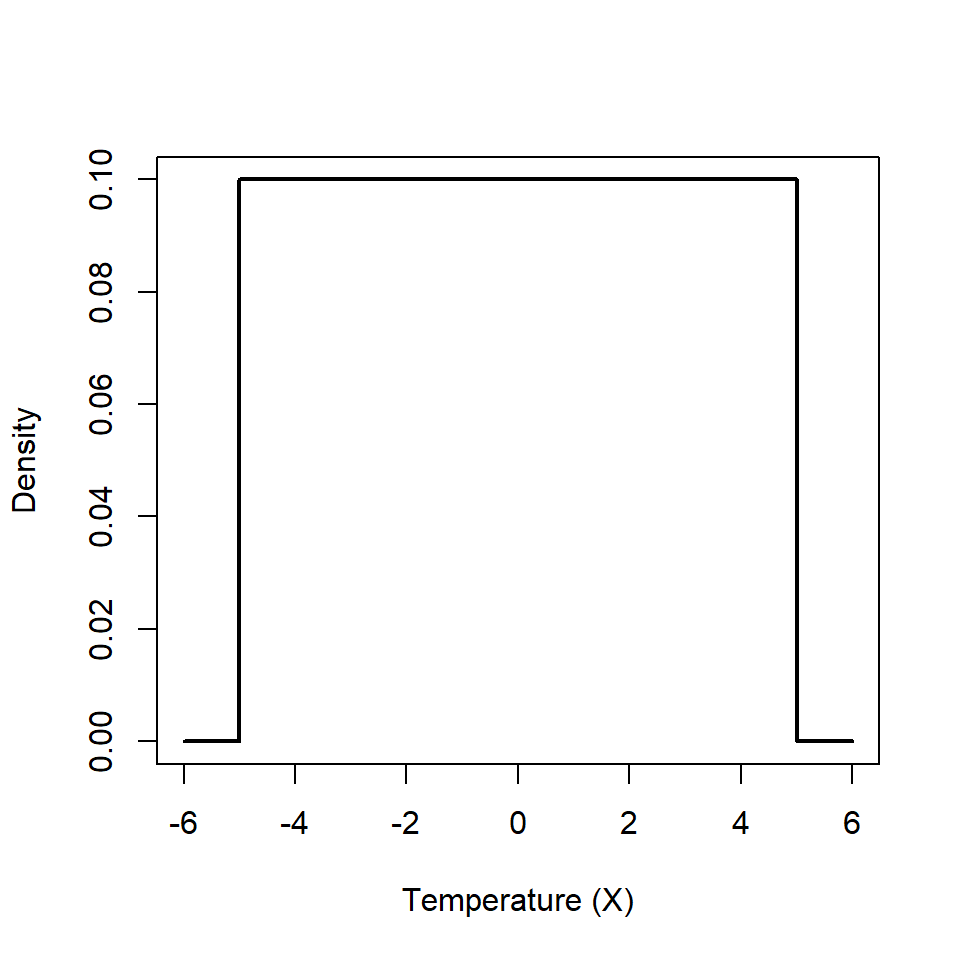
\includegraphics{IntroStats_files/figure-latex/pdfex1-1} 

}

\caption{Probability density function for the temperature of a chemical reaction.}\label{fig:pdfex1}
\end{figure}

We can verify that \(f(x)\) is a PDF by checking that it satisfies the two conditions noted above. The limits in this example are {[}-5, 5{]} and we can see that \(f(x)=0.1\) on this interval which satisfies the first condition. The second condition requires a bit more work because we need to integrate the function between these limits (this is just for illustration):

\[\int _{-5}^{5} f(x)dx = \int _{-5}^{5} 0.1 dx = 0.1[x ]_{-5}^5 = 0.1(5 - -5) = 0.1 \times 10 = 1\]

Thus the area under the curve equals 1 and thus satisfies condition 2.

For a discrete random variable, the PMF defined the probability associated with a certain outcome and the sum of the probabilities for all outcomes equalled one. We have just seen that for a continuous random variable, integration of the PDF over all possible values also equals one (condition 2). Therefore, to obtain the probability associated with a range of specified values, we integrate the PDF over the range of the specified values - hence, equation 7.1.

For example, the probability that \(X\) is between -2.5 and 2.5 is given by:

\[Pr(-2.5 \le X \le 2.5) = \int_{-2.5}^{2.5} 0.1 \mathrm{d}x \]

\[ = 0.1[x]_{-2.5}^{2.5} = 0.1[2.5 - -2.5] = 0.1 \times 5 = 0.5\]

With a discrete random variable, the probability associated with a particular value (\(Pr(X=x)\)) can be calculated. This is not the same for a continuous random variable and only the probability for a range of possible values can be calculated. Think about a distribution of a continuous variable such as height (denoted by \(H\)); the probability that someone is between 165-166 cm can be found from

\[Pr(165 \le H \le 166) = \int_{165}^{166} f(h)dh \]

If the interval of interest reduces, say \(Pr(165 \le H \le 165.5)\), then it follows that the probability will also reduce. As the interval gets narrower the probability will also reduce until the interval is so precise that the probability is effectively zero and hence, the probability of a particular value is zero. Thus for continuous distributions, only intervals are considered.

\hypertarget{cumulative-distribution-function-1}{%
\subsection{Cumulative distribution function}\label{cumulative-distribution-function-1}}

The cumulative distribution function, (CDF), for a continuous random variable is the same as for a discrete random variable, i.e.~
\[ F(x) = Pr(X \leq x) \]

However, while the calculation of the CDF involves summation for a discrete random variable it involves integration for a continuous random variable. For example, the probability that the temperature is less than 0 is given by:

\[ F(x) = Pr(X \leq 0) = \int_{-5}^{0} 0.1 \mathrm{d}x \]

\[ = 0.1[x]_{-5}^{0} = 0.1[0 - -5] = 0.1 \times 5 = 0.5 \]

This calculation is shown to illustrate how the probability is obtained. In practice, we will use R to do the calculations because integrating some of the specific distributions we will consider is a non-trivial task.

\hypertarget{doing-this-in-r-6}{%
\subsubsection{Doing this in R}\label{doing-this-in-r-6}}

As with the binomial distribution shown in the previous chapter, there are functions which can be used to calculate probabilities for a uniform distribution; not surprisingly, the functions have the suffix \texttt{unif}. To define a uniform function, the minimum and maximum values are required (in this example of a chemical reaction, these are -5 and 5, respectively).

\begin{Shaded}
\begin{Highlighting}[]
\CommentTok{\# Create a range of values (make wider than limits of the distribution)}
\NormalTok{xvalues }\OtherTok{\textless{}{-}} \FunctionTok{seq}\NormalTok{(}\SpecialCharTok{{-}}\DecValTok{6}\NormalTok{, }\DecValTok{6}\NormalTok{, }\AttributeTok{by=}\FloatTok{0.01}\NormalTok{)}
\CommentTok{\# Create a dataframe}
\NormalTok{results }\OtherTok{\textless{}{-}} \FunctionTok{data.frame}\NormalTok{(}\AttributeTok{x=}\NormalTok{xvalues)}
\CommentTok{\# Calculate density specifying limits of distribution }
\NormalTok{results}\SpecialCharTok{$}\NormalTok{density }\OtherTok{\textless{}{-}} \FunctionTok{dunif}\NormalTok{(}\AttributeTok{x=}\NormalTok{results}\SpecialCharTok{$}\NormalTok{x, }\AttributeTok{min=}\SpecialCharTok{{-}}\DecValTok{5}\NormalTok{, }\AttributeTok{max=}\DecValTok{5}\NormalTok{) }
\CommentTok{\# Plot PDF}
\FunctionTok{plot}\NormalTok{(results}\SpecialCharTok{$}\NormalTok{x, results}\SpecialCharTok{$}\NormalTok{density, }\AttributeTok{type=}\StringTok{"l"}\NormalTok{, }\AttributeTok{xlab=}\StringTok{"x"}\NormalTok{, }\AttributeTok{ylab=}\StringTok{"Density"}\NormalTok{)}
\end{Highlighting}
\end{Shaded}

\begin{center}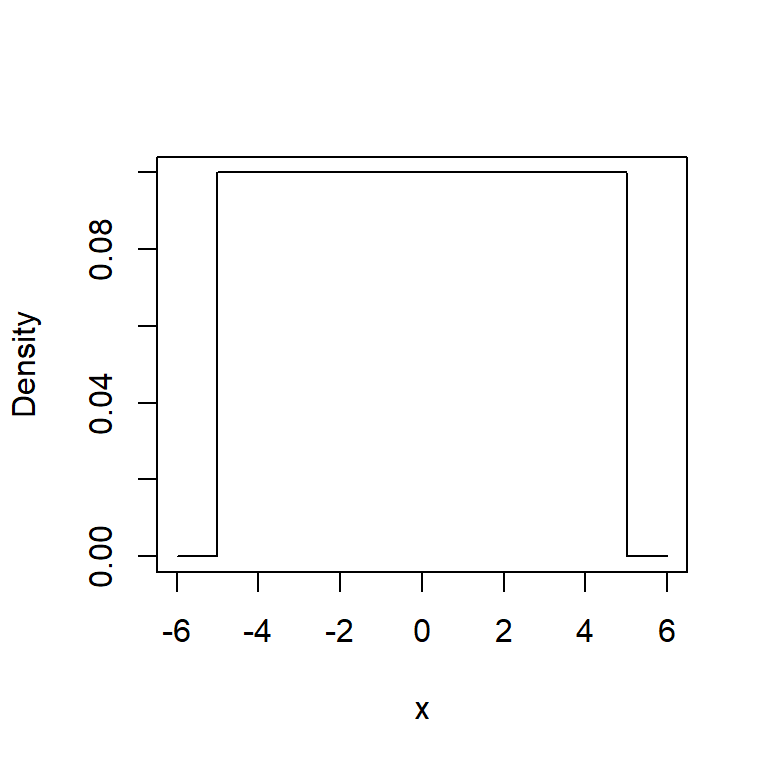
\includegraphics{IntroStats_files/figure-latex/unnamed-chunk-31-1} \end{center}

\begin{Shaded}
\begin{Highlighting}[]
\CommentTok{\# Calculate CDF}
\NormalTok{results}\SpecialCharTok{$}\NormalTok{CDF }\OtherTok{\textless{}{-}} \FunctionTok{punif}\NormalTok{(}\AttributeTok{q=}\NormalTok{results}\SpecialCharTok{$}\NormalTok{x, }\AttributeTok{min=}\SpecialCharTok{{-}}\DecValTok{5}\NormalTok{, }\AttributeTok{max=}\DecValTok{5}\NormalTok{)}
\CommentTok{\# Plot CDF}
\FunctionTok{plot}\NormalTok{(results}\SpecialCharTok{$}\NormalTok{x, results}\SpecialCharTok{$}\NormalTok{CDF, }\AttributeTok{type=}\StringTok{"l"}\NormalTok{, }\AttributeTok{xlab=}\StringTok{"x"}\NormalTok{, }\AttributeTok{ylab=}\StringTok{"CDF"}\NormalTok{)}
\end{Highlighting}
\end{Shaded}

\begin{center}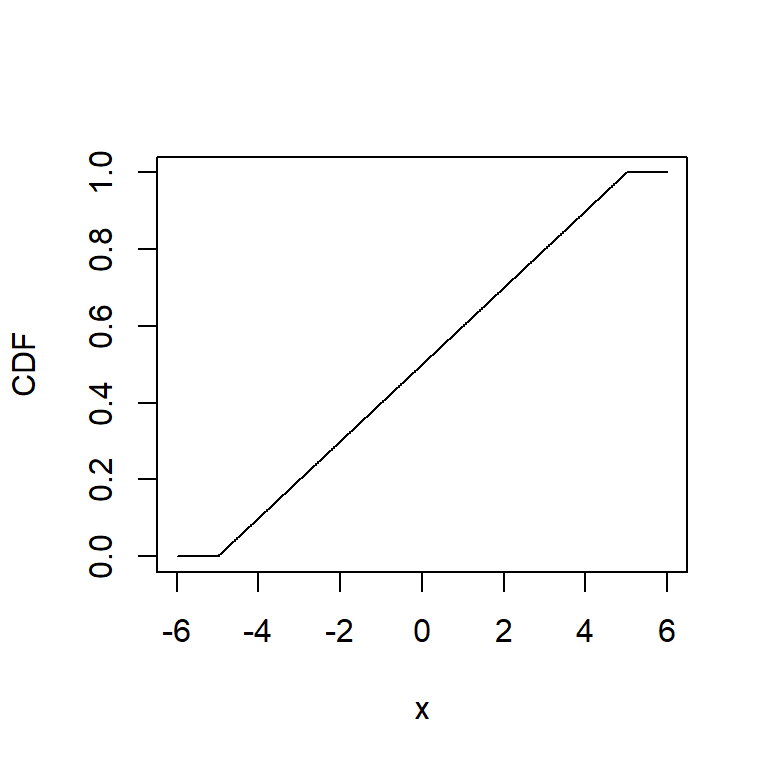
\includegraphics{IntroStats_files/figure-latex/unnamed-chunk-31-2} \end{center}

\hypertarget{expectation-and-variance-1}{%
\subsection{Expectation and variance}\label{expectation-and-variance-1}}

Similar to a discrete random variable, the expectation for a continuous random variable is like a weighted sum, but this time integration is required.

\begin{align}
E(X) = \int_{-\infty}^{\infty}xf(x)dx
\end{align}

Likewise the variance is given by,

\begin{align}
Var(X) = \int_{-\infty}^{\infty}(x - E(X))^2f(x)dx
\end{align}

which is equivalent to

\begin{align}
Var(X) = E(X^2) - [E(X)]^2
\end{align}

\textbf{Example} In the chemical reaction, the expected value is given by

\[E(X) = \int_{-5}^{5} x0.1 dx\]
\[ =0.1[\frac{x^2}{2}]_{-5}^{5} = \frac{0.1}{2}[25 - 25] = 0 \]
Thus, the expected temperature in the chemical reaction is 0; this makes sense if we look at Figure \ref{fig:pdfex1} - it is the central value of \(X\).

\hypertarget{special-continuous-distributions}{%
\section{Special continuous distributions}\label{special-continuous-distributions}}

An example of a uniform distribution has just been introduced. There are several other distributions that will crop up later in the course, specifically the normal, \(t\) and \(F\) distributions.

These theoretical distributions are characterised by parameters which describe the location, scale and shape of the curve. In general, the properties of these parameters are as follows:

\begin{itemize}
\item
  location fixes the lower, or mid, point of the distribution on the number scale or \(x\)-axis (e.g.~is the midpoint of the distribution at 10 or 100 etc.),
\item
  scale determines length of the \(x\)-axis (e.g.~how spread out the distribution is along the \(x\)-axis),
\item
  shape allows the curve to take a variety of shapes, perhaps shifting or stretching the distribution along the \(x\)-axis.
\end{itemize}

Not all distributions have all these parameters and the distributions described in this document are characterised by only one or two parameters. The normal distribution is used for many applications and so we look at this distribution in detail.

\hypertarget{normal-distribution}{%
\subsection{normal distribution}\label{normal-distribution}}

A normally distributed random variable \(X\) is defined by two parameters, \(\mu\) and \(\sigma^2\), where \(\mu=E(X)\) and \(\sigma^2=Var(X)\). This can be written more concisely as \(X \sim N(\mu, \sigma^2)\). The normal distribution is symmetrical and the parameter \(\mu\) defines the centre of the distribution and \(\sigma^2\) defines the spread.

How different values of \(\mu\) and \(\sigma^2\) affect the shape of the distribution can be seen in Figure \ref{fig:pdfnormex1}. Note that, because of condition 2, the area under all the curves is one and so there is a trade-off between the maximum density of the distribution and how spread out the distribution is along the \(x\)-axis.



\begin{figure}

{\centering 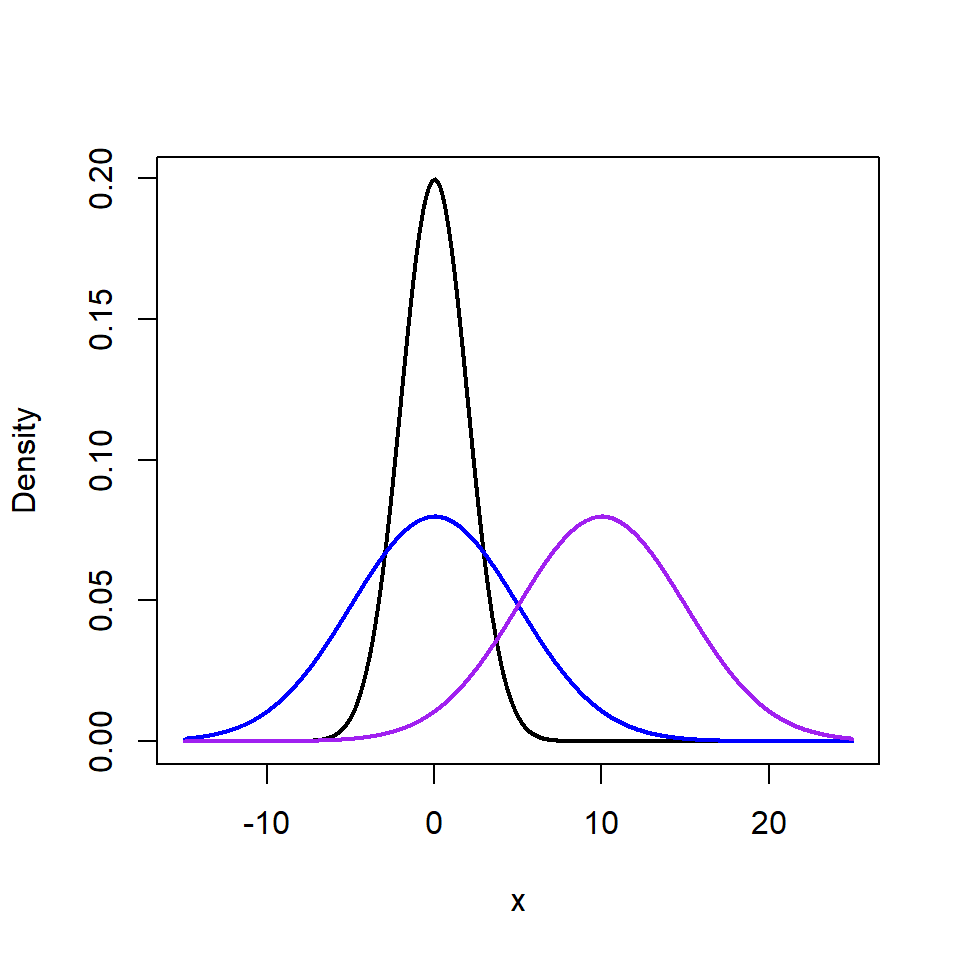
\includegraphics{IntroStats_files/figure-latex/pdfnormex1-1} 

}

\caption{Examples of normal distributions with different values of \(\mu\) and \(\sigma^2\); \(N(0,4)\) (black), \(N(0,25)\) (blue), \(N(10, 25)\) (purple).}\label{fig:pdfnormex1}
\end{figure}

The probability distribution function for the normal distribution is given by:

\begin{align}
f(x; \mu, \sigma) = \frac{1}{\sqrt{2\pi\sigma^2}}e^{[\frac{-1}{2\sigma^2}(x-\mu)^2]}
\end{align}

Normal distributions have some useful properties (which we make use of in future chapters):

\begin{itemize}
\item
  they are symmetric about the mean and median (which are equal)
\item
  68\% of observations are within \(\pm 1 \times \sigma\) of \(\mu\) (i.e.~68\% of the area is within the interval \(\mu-\sigma\) and \(\mu + \sigma\))
\item
  95\% of observations are within \(\pm 1.96 \times \sigma\) of \(\mu\)
\item
  99\% of observations are within \(\pm 2.58 \times \sigma\) of \(\mu\)
\end{itemize}

This can be seen in Figure \ref{fig:pdfnormex2}.



\begin{figure}

{\centering 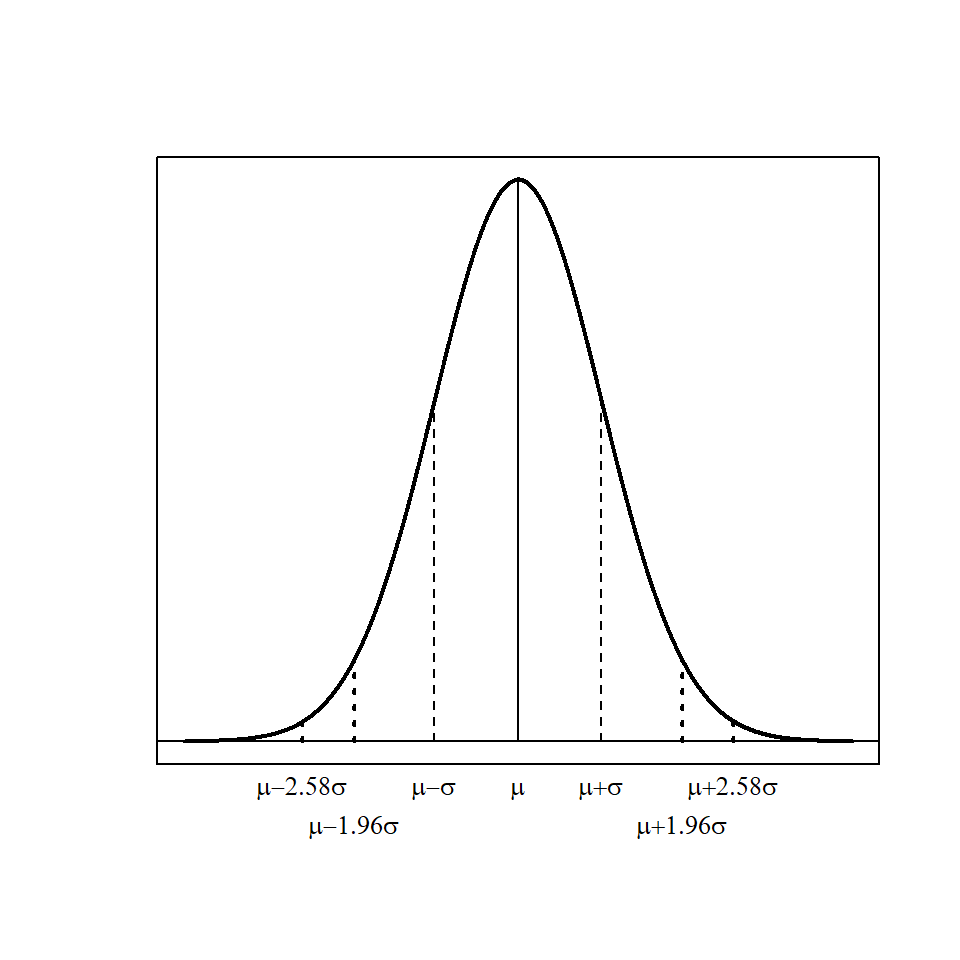
\includegraphics{IntroStats_files/figure-latex/pdfnormex2-1} 

}

\caption{(ref:pdfnormex2}\label{fig:pdfnormex2}
\end{figure}

\hypertarget{doing-calculations-in-r}{%
\subsubsection{Doing calculations in R}\label{doing-calculations-in-r}}

Many measurements will have empirical frequency distributions that are normal, or nearly normal. This can be helpful in that we can then use this information to find out about the population, given knowledge of \(\mu\) and \(\sigma\). Remember that condition 2 specifies that the area under \(f(x)\) for all possible values of \(X\) is equal to one (there is an equivalent condition for discrete random variables), hence the area of different intervals can inform us about the probability of these intervals.

For example, assume the distribution of women's heights (\(X\)) is approximately normal with a mean 160cm and standard deviation 6cm (i.e.~\(X \sim N(160, 6^2)\)). We want to find the probability that a randomly chosen woman is smaller than 150cm (\(Pr(X \le 150)\)) and this is given by the area under the curve less than 150 cm (Figure \ref{fig:pdfnormex3}).



\begin{figure}

{\centering 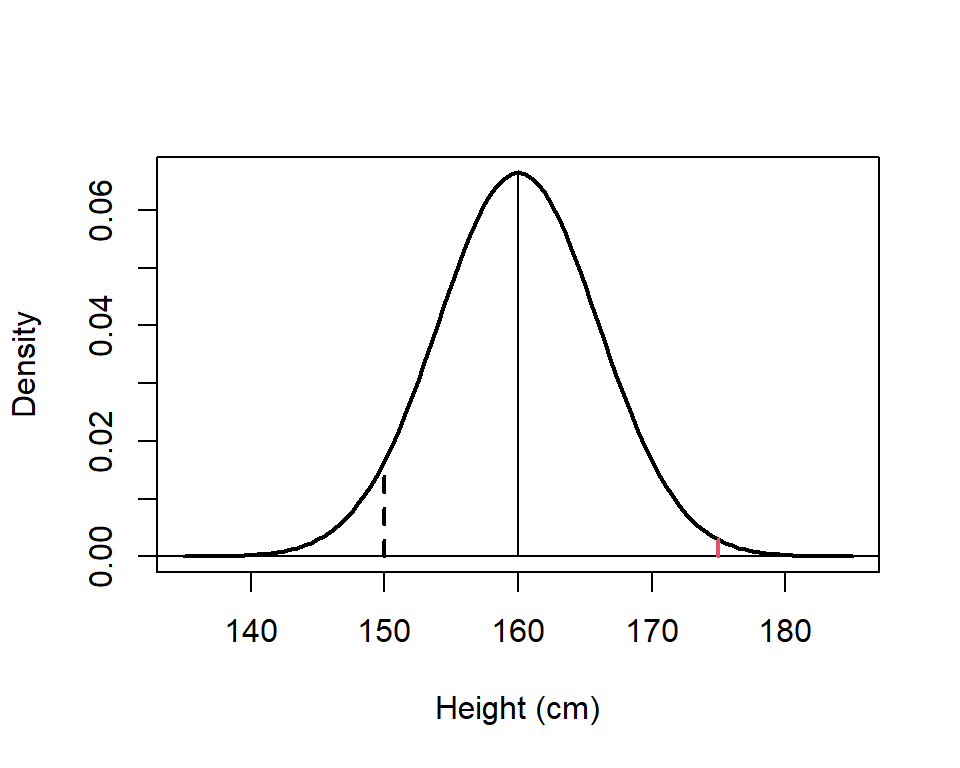
\includegraphics{IntroStats_files/figure-latex/pdfnormex3-1} 

}

\caption{ref:pdfnormex3}\label{fig:pdfnormex3}
\end{figure}

As we have seen, we can find this from the cumulative distribution function and we can use R to do the calculations:

\begin{Shaded}
\begin{Highlighting}[]
\CommentTok{\# Specify parameters}
\NormalTok{mu }\OtherTok{\textless{}{-}} \DecValTok{160} \CommentTok{\# Mean}
\NormalTok{sigma }\OtherTok{\textless{}{-}} \DecValTok{6} \CommentTok{\# Standard deviation}
\CommentTok{\# CDF {-} area under the curve less than q}
\FunctionTok{pnorm}\NormalTok{(}\AttributeTok{q=}\DecValTok{150}\NormalTok{, }\AttributeTok{mean=}\NormalTok{mu, }\AttributeTok{sd=}\NormalTok{sigma, }\AttributeTok{lower.tail=}\ConstantTok{TRUE}\NormalTok{)}
\end{Highlighting}
\end{Shaded}

\begin{verbatim}
[1] 0.04779035
\end{verbatim}

The probability is 0.04779, hence, approximately 4.78\% of women will be less than 150 cm.

What about the probability that a randomly chosen women will be greater than 175 cm (i.e.~\(Pr(X > 175)\))? In this case we want the area under the curve for values greater than 175 (red line in Figure \ref{fig:pdfnormex3}). Again we can use R to do the calculations and there are two possible options. The first calculation uses the complement rule and the CDF. Hence,

\[Pr(X > 175) = 1 - Pr(X \le 175)\]
In R, the command is:

\begin{Shaded}
\begin{Highlighting}[]
\DecValTok{1} \SpecialCharTok{{-}} \FunctionTok{pnorm}\NormalTok{(}\AttributeTok{q=}\DecValTok{175}\NormalTok{, }\AttributeTok{mean=}\NormalTok{mu, }\AttributeTok{sd=}\NormalTok{sigma)}
\end{Highlighting}
\end{Shaded}

\begin{verbatim}
[1] 0.006209665
\end{verbatim}

We can be somewhat casual about \(\le\) and \(<\) (and also \(\ge\) and \(>\)) signs because as we have seen the \(Pr(X=a) = 0\). (Note, this does not apply to discrete random variables.)

R provides an alternative method to obtain \(Pr(X > 175)\), if an additional argument is specified in the \texttt{pnorm} function. By default, the area to the left of a specified value (\texttt{q}), or the lower tail (i.e.~the CDF), is returned by \texttt{pnorm}. Specifying the argument \texttt{lower.tail=FALSE} will return the area to the right of \texttt{q} (the upper tail), hence, we can obtain the relevant probability directly:

\begin{Shaded}
\begin{Highlighting}[]
\CommentTok{\# Area under curve greater than q}
\FunctionTok{pnorm}\NormalTok{(}\AttributeTok{q=}\DecValTok{175}\NormalTok{, }\AttributeTok{mean=}\NormalTok{mu, }\AttributeTok{sd=}\NormalTok{sigma, }\AttributeTok{lower.tail=}\ConstantTok{FALSE}\NormalTok{)}
\end{Highlighting}
\end{Shaded}

\begin{verbatim}
[1] 0.006209665
\end{verbatim}

These functions make calculating probabilities relatively straight forward, for example, we can find the probability a women is between 148 and 172 cm, i.e.~\(Pr(148 \le X \le 172)\).

\begin{Shaded}
\begin{Highlighting}[]
\CommentTok{\# Area under curve in interval 148 to 172}
\NormalTok{area172 }\OtherTok{\textless{}{-}} \FunctionTok{pnorm}\NormalTok{(}\AttributeTok{q=}\DecValTok{172}\NormalTok{, }\AttributeTok{mean=}\NormalTok{mu, }\AttributeTok{sd=}\NormalTok{sigma, }\AttributeTok{lower.tail=}\ConstantTok{TRUE}\NormalTok{)}
\NormalTok{area148 }\OtherTok{\textless{}{-}} \FunctionTok{pnorm}\NormalTok{(}\AttributeTok{q=}\DecValTok{148}\NormalTok{, }\AttributeTok{mean=}\NormalTok{mu, }\AttributeTok{sd=}\NormalTok{sigma, }\AttributeTok{lower.tail=}\ConstantTok{TRUE}\NormalTok{)}
\NormalTok{area172 }\SpecialCharTok{{-}}\NormalTok{ area148}
\end{Highlighting}
\end{Shaded}

\begin{verbatim}
[1] 0.9544997
\end{verbatim}

Why is this probability not surprising? Hint, how many values of \(\sigma\) are these limits away from the mean?

The interval 148 to 172 is \(\mu \pm 2 \sigma\) and we know that for a normal distribution, 95\% of the distribution falls within 1.96 standard deviations of the mean. Hence, we would expect the probability to be very close to 95\%.

\hypertarget{standard-normal-distribution}{%
\subsection{Standard normal distribution}\label{standard-normal-distribution}}

A special case of the normal distribution is the \textbf{standard normal distribution} where \(\mu=0\) and \(\sigma^2=1\). The PDF is simpler:

\begin{align}
f(x; \mu, \sigma) = \frac{1}{\sqrt{2\pi}}e^{\frac{(x - \mu)^2}{2}}
\end{align}

The standard normal distribution is very useful because any given normal distribution can be transformed to a standard normal PDF by converting the normal random variables to standard units. This process, called standardization, is simply

\begin{align}
Z = \frac{X - \mu}{\sigma}
\end{align}

A random variable from a standard normal distribution is often denoted by \(Z\), i.e \(Z \sim N(0, 1)\). Sometimes the term `normalisation' is used instead of standardisation but they refer to different transformations: normalisation usually means to scale the data values so they they lie between 0 and 1; standardisation transforms the data to have a mean 0 and standard deviation of one.

\textbf{Example} Assume that IQ (intellgent quotient) is distributed as \(N(100,15^2)\). What is the IQ for someone at the 99th percentile i.e.~what is \(q\) such that \(Pr(X \le X q)=0.99\)?

We can find this value using the CDF function in R.

\begin{Shaded}
\begin{Highlighting}[]
\FunctionTok{qnorm}\NormalTok{(}\AttributeTok{p=}\FloatTok{0.99}\NormalTok{, }\AttributeTok{mean=}\DecValTok{100}\NormalTok{, }\AttributeTok{sd=}\DecValTok{15}\NormalTok{)}
\end{Highlighting}
\end{Shaded}

\begin{verbatim}
[1] 134.8952
\end{verbatim}

Alternatively, we can find the 99th percentile for the standard normal, then multiply by \(\sigma\) and add \(\mu\) i.e.~

\[ X = Z \sigma + \mu\]

\begin{Shaded}
\begin{Highlighting}[]
\CommentTok{\# Use standard normal and transform}
\FunctionTok{qnorm}\NormalTok{(}\AttributeTok{p=}\FloatTok{0.99}\NormalTok{, }\AttributeTok{mean=}\DecValTok{0}\NormalTok{, }\AttributeTok{sd=}\DecValTok{1}\NormalTok{)}\SpecialCharTok{*}\DecValTok{15} \SpecialCharTok{+} \DecValTok{100}
\end{Highlighting}
\end{Shaded}

\begin{verbatim}
[1] 134.8952
\end{verbatim}

Thus, the IQ for someone in the 99th percentile will be nearly 135.

\hypertarget{simple-transformations-of-random-variables}{%
\subsection{Simple transformations of random variables}\label{simple-transformations-of-random-variables}}

Sometimes we may wish to consider transformations of random variables other than standardisation; for example a variable has been measured in some unit (e.g.~inches) and we want to transform it to another unit of measurement (e.g.~centimetres) and find the expected value in the new units of measurement.

There are some simple rules that we can apply in these cases which apply for both continuous and discrete random variables.

\hypertarget{adding-and-multipling-by-a-constant}{%
\subsubsection{Adding and multipling by a constant}\label{adding-and-multipling-by-a-constant}}

Let \(X\) be a random variable and let \(Y\) be some function of \(X\) that involves either the addition of some constant \(a\), the multiplication of a constant \(b\) or indeed both. The expected value of \(Y\), \(E(Y)\) can then be found using these simple rules:

\begin{itemize}
\item
  \(Y = aX\) and \(E(Y) = aE(X)\).
\item
  \(Y = X + b\) and \(E(Y) = E(X) + b\).
\item
  \(Y = aX + b\) and \(E(Y)= aE(X) + b\).
\end{itemize}

\textbf{Example} The expected temperature at a particular location was \(10^o\)Celsius. What is the expected value in Fahrenheit?

The conversion from Celsius (\(C\)) to Fahrenheit (\(F\)) is
\[ F = 1.8C + 32\]
Therefore, the expected value in Fahrenheit is given by:

\[E(F) = 1.8E(C) + 32 = 1.8 \times 10 + 32 = 50\]
Hence, the expected value in Fahrenheit is 50\(^o\).

What about the variance of a simple transformation? Similar rules to those for the expectation also apply:

\begin{itemize}
\item
  \(Y = aX\) then \(Var(Y)= a^2Var(X)\)
\item
  \(Y = X + b\) then \(Var(Y)= Var(X)\)
\item
  \(Y = aX + b\) then \(Var(Y)= a^2Var(X)\).
\end{itemize}

If a constant is added to, or subtracted from, \(X\), then the expected value is shifted by this amount but the variability is unchanged. Conversely, if a variable is multiplied by a constant, the expected value is also multiplied by the constant and the variance is multiplied by the constant squared.

We can illustrate these rules empirically by generating some random data. Here we generate data for a variable \(X \sim N(\mu=20, \sigma^2=9)\).

\begin{Shaded}
\begin{Highlighting}[]
\CommentTok{\# Set seed}
\FunctionTok{set.seed}\NormalTok{(}\DecValTok{1234}\NormalTok{)}
\CommentTok{\# Generate 100 random values from a normal distribution (with mean 20 and sd 3)}
\NormalTok{X }\OtherTok{\textless{}{-}} \FunctionTok{rnorm}\NormalTok{(}\AttributeTok{n=}\DecValTok{100}\NormalTok{, }\AttributeTok{mean=}\DecValTok{20}\NormalTok{, }\AttributeTok{sd=}\DecValTok{3}\NormalTok{)}
\CommentTok{\# Expected value and variance of X}
\FunctionTok{mean}\NormalTok{(X)}
\end{Highlighting}
\end{Shaded}

\begin{verbatim}
[1] 19.52971
\end{verbatim}

\begin{Shaded}
\begin{Highlighting}[]
\FunctionTok{var}\NormalTok{(X)}
\end{Highlighting}
\end{Shaded}

\begin{verbatim}
[1] 9.07947
\end{verbatim}

The transformation is specified \(Y = 2X + 5\) and so we create \(Y\) and then obtain the mean and variance using the usual R functions.

\begin{Shaded}
\begin{Highlighting}[]
\CommentTok{\# Let Y = 2X + 5}
\NormalTok{Y }\OtherTok{\textless{}{-}}\NormalTok{ (}\DecValTok{2} \SpecialCharTok{*}\NormalTok{ X) }\SpecialCharTok{+} \DecValTok{5}
\CommentTok{\# Expected value and variance of Y}
\FunctionTok{mean}\NormalTok{(Y)}
\end{Highlighting}
\end{Shaded}

\begin{verbatim}
[1] 44.05943
\end{verbatim}

\begin{Shaded}
\begin{Highlighting}[]
\FunctionTok{var}\NormalTok{(Y)}
\end{Highlighting}
\end{Shaded}

\begin{verbatim}
[1] 36.31788
\end{verbatim}

Thus, the mean of \(Y\) is 44.06 and the variance is 36.32. Now, we use the rules above to obtain the mean and variance of \(Y\) from the mean and variance of \(X\), \(E(X)\) and \(Var(X)\):

\begin{Shaded}
\begin{Highlighting}[]
\CommentTok{\# Use rules to obtain expected value of y}
\NormalTok{(}\DecValTok{2}\SpecialCharTok{*}\FunctionTok{mean}\NormalTok{(X)) }\SpecialCharTok{+} \DecValTok{5}
\end{Highlighting}
\end{Shaded}

\begin{verbatim}
[1] 44.05943
\end{verbatim}

\begin{Shaded}
\begin{Highlighting}[]
\CommentTok{\# and variance}
\DecValTok{4}\SpecialCharTok{*}\FunctionTok{var}\NormalTok{(X)}
\end{Highlighting}
\end{Shaded}

\begin{verbatim}
[1] 36.31788
\end{verbatim}

The same values were obtained as before; the other rules can be similarly demonstrated.

\hypertarget{adding-random-variables}{%
\subsubsection{Adding random variables}\label{adding-random-variables}}

Sometimes we may wish to consider a transformation including two random variables, \(X\) and \(Y\). In this case, the expected value for adding the variables, (\(X + Y\)), is given by:

\begin{align}
E(X + Y) = E(X) + E(Y)
\end{align}

Similarly, the expected value for subtracting the variables, \((X-Y)\), is given by:

\begin{align}
E(X - Y) = E(X) - E(Y)
\end{align}

If we assume that \(X\) and \(Y\) are independent, the variances can simply be added to obtain both \(Var(X+Y)\) and \(Var(X-Y)\):

\begin{align}
Var(X+Y) = Var(X-Y) = Var(X) + Var(Y)
\end{align}

More complicated transformations can be considered using previous rules, for example,

\[Z = a + bX + cY\]
Hence,

\begin{align}
E(Z) = a + bE(X) + cE(Y)
\end{align}

and, similarly if \(X\) and \(Y\) are independent, the variance is given by

\begin{align}
Var(Z) = b^2Var(X) + c^2Var(Y)
\end{align}

\textbf{Example} A time-and-motion study measures the time required for an assembly line worker to perform two successive repetitive tasks. The data showed that the time required to position a part on an automobile chassis varied from car to car with mean 11 seconds and standard deviation 2 seconds. The time required to attach the part to the chassis also varied, with mean 20 seconds and standard deviation 4 seconds. What is the expected combined time for positioning and attaching the part?

To answer this, let \(X\) represent the time to position the part and \(Y\) represent the time to attach the part. The expected total time taken to position and attach a part, \(X+Y\), is given by:

\[ E(X+Y) = E(X) + E(Y) = 11 + 20 = 31 \textrm{ seconds}\]

The time-and-motion study finds that the times required for the two steps are independent, i.e.~the time to attach a part is not affected by the time taken to position the part. What is the standard deviation for the time to position and attach the part?

\[V(X+Y) = V(X) + V(Y) = 2^2 + 4^2 = 20 \]

\[SD(X+Y) = \sqrt{V(X+Y)} = \sqrt{20} = 4.47 \textrm{ seconds}\]

So far we have considered variables that are independent but if this is not the case, then we need to take into account how closely related they are.

\hypertarget{covariance-and-correlation}{%
\subsubsection{Covariance and correlation}\label{covariance-and-correlation}}

If \(X\) and \(Y\) are not independent, then the covariance, \textbf{a measure of the degree of association} or \textbf{similarity}, of \(X\) and \(Y\), needs to be taken into account when calculating the variance:

\begin{align}
Var(X+Y) = Var(X) + Var(Y) + 2Cov(X,Y) \\
Var(X-Y) = Var(X) + Var(Y) - 2Cov(X,Y)
\end{align}

The covariance is explored further but first another useful rule theorem is required.

If two independent random variables are multiplied, the expected value of the product is the product of the expected values, or more succinctly:

\begin{align}
E(XY) = E(X)E(Y)
\end{align}

The covariance between two random variables \(X\) and \(Y\) is:

\begin{align}
Cov(X,Y) = E[(X-E(X))(Y-E(Y))] \\
= E(XY) - E(X)E(Y)
\end{align}

Independent random variables have zero covariance.

A related measure is the correlation coefficient, \(\rho\), which measures the linear relationship between two variables:

\begin{align}
\rho = \frac{Cov(X,Y)}{\sqrt{Var(X)Var(Y)}}
\end{align}

Correlation is explored further in Chapter \ref{correlation} and so it is not expanded on here, except to say that \(\rho\) (or denoted by \(r\) for a sample) can take values between -1 and 1 (inclusive) and when \(\rho=1\), there is a positive linear relationship between \(X\) and \(Y\), when \(\rho=-1\), there is a negative relationship between \(X\) and \(Y\) and when \(\rho=0\), there is no relationship between \(X\) and \(Y\).

We can rearrange equation 17 so that

\[Cov(X,Y) = \rho \sqrt{Var(X)Var(Y)}\]

and then substitute into equations, such that

\begin{align}
Var(X+Y) = Var(X) + Var(Y) + 2\rho \sqrt{Var(X)Var(Y)} \\
Var(X-Y) = Var(X) + Var(Y) - 2\rho \sqrt{Var(X)Var(Y)}
\end{align}

\textbf{Example} How would the standard deviation change, if the time taken to position and attach a part were dependent, with a correlation coefficient of 0.8?

\[Var(X+Y) = Var(X) + Var(Y) + 2\rho\sqrt{Var(X)Var(Y)}\]

\[ =2^2 + 4^2 + 2 \times 0.8 \times \sqrt{2^2 \times 4^2} = 32.8\]
\[SD(X+Y) = \sqrt{32.8} = 5.73 \textrm{ seconds}\]
\textbf{Q6.1} Using the time-and-motion study described in the example, the variation in the worker's performance is reduced by better training, and hence the standard deviations of positioning and attaching the parts has decreased. Will this decrease change the expected value of the combined steps, if the mean times for the two steps remain as before?

\textbf{Q6.2} A company makes a profit of \pounds 2,000 on each military unit sold and \pounds 3,500 on each civilian unit. Thus the profit is from military units is \pounds 2,000\(X\) where \(X\) is the number of military units sold; similarly, the profit from civilian units is \pounds 3,500\(Y\), where \(Y\) is the number of civilian units sold. The expected number of military units to be sold is 5,000 and the expected number of civilian units to be sold is 445. Using this information answer the following questions.

\textbf{a.} What is the expected profit on military units?

\textbf{b.} What is the expected total profit for military and civilian units?

\textbf{c.} What is the expected difference in profit between military and civilian units?

\textbf{d.} Assuming that the number of military and civilian units sold are independent, describe how to calculate the variance of the total profit. Will this be different to the variance of the difference calculated in part c?

\textbf{Q6.3} Planks of wood are cut into two sizes, short and long. The length (in metres) of the short planks has a \(N(0.5, 0.01)\) distribution and the length of the long planks has a \(N(1.5, 0.0625)\) distribution. It was found that one short plank and two long planks placed end to end were required to make one floorboard.

\textbf{a.} What is the mean length of floorboards?

\textbf{b.} Assuming that the two lengths of plank are independent, what is the variance of the floorboard.

\textbf{c.} What is the probability that the floorboard will be too long for a room 4 metres in length?

\hypertarget{SUMcontrv}{%
\section{Summary}\label{SUMcontrv}}

There are analogous functions to the PMF and CDF for continuous random variables, the main difference is that we need to integrate under the curves to obtain probabilities, expected values and variances rather than summation.

The normal and standard normal distributions have been described in detail. These distributions crop up frequently in statistics; other distributions considered in following chapters are the \(t\) and \(F\).

Random variables can be transformed in various ways and there are simple rules which can be applied to obtain the expected values and variances of these transformations.

\hypertarget{learning-outcomes-2}{%
\subsection{Learning outcomes}\label{learning-outcomes-2}}

In this chapter, you have learnt definitions for the

\begin{enumerate}
\def\labelenumi{\arabic{enumi}.}
\item
  PDF and CDF
\item
  expectation and variance
\end{enumerate}

for continuous random variables. The normal and standard normal distributions have been described in detail and rules for obtaining the expected value and variances for simple transformations of random variables have been illustrated.

\hypertarget{ANScontrv}{%
\section{Answers}\label{ANScontrv}}

\textbf{Q6.1} No.~Changing the standard deviations will not change the means.

\textbf{Q6.2} \textbf{a.} Consider \(X_T = 2000X\), then using
\[E(X_T) = 2000E(X) = 2000 \times 5000 = 10000000\]

the expected profit is \(\pounds 10,000,000\).

\textbf{Q6.2} \textbf{b.} The expected total profit is obtained from

\[ E(2000X+3500Y) = 2000E(X) + 3500E(Y) = 2000 \times 5000 + 3500 \times 445 = 11557500 \]
Hence, the expected total profit is £\(11,557,500\).

\textbf{Q6.2} \textbf{c.} The expected difference in profits between military and civilian sales can be calculated from

\[E(2000X - 3500Y) = 2000E(X) - 3500E(Y) = 2000 \times 5000 - 3500 \times 445 = 8442500\]
Thus, the expected difference in profits is £8,442,500.

\textbf{Q6.2} \textbf{d.} The variance for \(2000X\) units is given by \(Var(2000X) = 2000^2Var(X)\) and similarly the variance for \(3500Y\) is \(Var(3500Y) = 3500^2Var(Y)\).

If the units sold for military and civilian use are independent, then the variances can be added to calculate the variance of the total profit:

\[Var(2000X + 3500Y) = 2000^2Var(X) + 3500^2Var(Y)\]
The variance will be the same for the difference in profits.

\textbf{Q6.3} Let \(X\) represent the short planks and \(Y\) represent the long planks and so a floorboard is made up of \(F = X + 2Y\).

\textbf{Q6.3} \textbf{a.} Using equation 11, let \(a=0\), \(b=1\) and \(c=2\),
\[E(F) = 1 \times E(X) + 2 \times E(Y) = 0.5 + 2 \times 1.5 = 3.5\]
The expected length of a floorboard is 3.5m.

\textbf{Q6.3} \textbf{b.} Similarly, the variance is given by
\[Var(F) = 1 \times Var(X) + 2^2Var(Y) = 0.01 + 4 \times 0.0625 = 0.26\]
\textbf{Q6.3} \textbf{c.} The probability \(Pr(F > 4)\) is required, where \(F \sim N(3.5, 0.26)\). R can be used to find this probability with the \texttt{pnorm} command. There are two equivalent commands:

Using \(1 - Pr(X \le 4)\)

\begin{Shaded}
\begin{Highlighting}[]
\DecValTok{1} \SpecialCharTok{{-}} \FunctionTok{pnorm}\NormalTok{(}\AttributeTok{q=}\DecValTok{4}\NormalTok{, }\AttributeTok{mean=}\FloatTok{3.5}\NormalTok{, }\AttributeTok{sd=}\FunctionTok{sqrt}\NormalTok{(}\FloatTok{0.26}\NormalTok{))}
\end{Highlighting}
\end{Shaded}

\begin{verbatim}
[1] 0.1633998
\end{verbatim}

Alternatively,

\begin{Shaded}
\begin{Highlighting}[]
\FunctionTok{pnorm}\NormalTok{(}\AttributeTok{q=}\DecValTok{4}\NormalTok{, }\AttributeTok{mean=}\FloatTok{3.5}\NormalTok{, }\AttributeTok{sd=}\FunctionTok{sqrt}\NormalTok{(}\FloatTok{0.26}\NormalTok{), }\AttributeTok{lower.tail=}\ConstantTok{FALSE}\NormalTok{)}
\end{Highlighting}
\end{Shaded}

\begin{verbatim}
[1] 0.1633998
\end{verbatim}

Therefore, the probability that a floorboard is greater than 4 m is 0.163.

\hypertarget{CIformean}{%
\chapter{Confidence intervals for sample means}\label{CIformean}}

\emph{\ldots{} a hypothesis test tells us whether the observed data are consistent with the null hypothesis, and a confidence interval tells us which hypotheses are consistent with the data.} William C. Blackwelder.

\hypertarget{INTci}{%
\section{Introduction}\label{INTci}}

We would like a sample to be representative of the target population. If we were to generate several samples from the same population and then calculate the sample statistics for each sample (e.g.~a mean), it is likely that the statistics would differ between samples - this is due to sampling error and is unavoidable. However, the extent to which these sample means will vary is somewhat predictable and we can use this information to provide a measure of uncertainty for the sample statistic. This takes the form of an interval between which we have some confidence that the true mean lies - this is called a confidence interval (CI). There are several methods which can be used to obtain a CI, depending on whether the data fulfill various criteria.

In this chapter you will:

\begin{itemize}
\tightlist
\item
  examine the behaviour of the sample mean
\item
  quantify the precision of the sample mean and hence calculate a confidence interval,
\item
  quantify the precision of the difference between two sample means and again calculate a confidence interval, and finally
\item
  consider an alternative approach for obtaining a confidence interval.
\end{itemize}

In this chapter we are mainly concerned with sample means but similar uncertainty will exist for other sample statistics such as the median, variance and proportions. In the final section we consider how the uncertainty of these other statistics can be quantified.

\hypertarget{uncertainty-of-the-sample-mean}{%
\section{Uncertainty of the sample mean}\label{uncertainty-of-the-sample-mean}}

To illustrate the variability in the sample, we consider the distribution of women's heights. Assume that height is normally distributed with a mean of 160 cm and a standard deviation of 6 cm, i.e.~Height \(\sim N(\mu=160, \sigma^2=6^2)\).

If we randomly draw five values from this distribution, then these might be:
\emph{152.7}, \emph{161.7}, \emph{166.6}, \emph{145.9} and \emph{162.6}

The mean of this sample is 157.9 cm and this is quite close to the population mean. Usually however, we don't know the population mean and so, in general, we want to know how well a sample mean represents the population. To find out how good an estimate is, we need to know how precise it is and this depends on:

\begin{itemize}
\tightlist
\item
  the sample size, and
\item
  the variability in the population.
\end{itemize}

Intuitively, we might expect that if the population is very variable, then the distribution of sample means may also be variable. Conversely, if the population is not very variable, then we might expect that sample means will be similar to the population mean and also to each other. In addition, a large sample may more closely resemble the population than a small sample and, hence, the sample mean from a large sample may be more similar to the population mean than the sample mean from a small sample.

This concept can be illustrated by generating many samples from a known population, calculating the mean for each sample and looking at the distribution of the sample means. In Figure (\ref{fig:histsampsize}), 1000 sample means have been generated from samples of different sizes, drawn from a normal distribution with mean 160 and standard deviation 6.

\begin{figure}[!htb]

{\centering 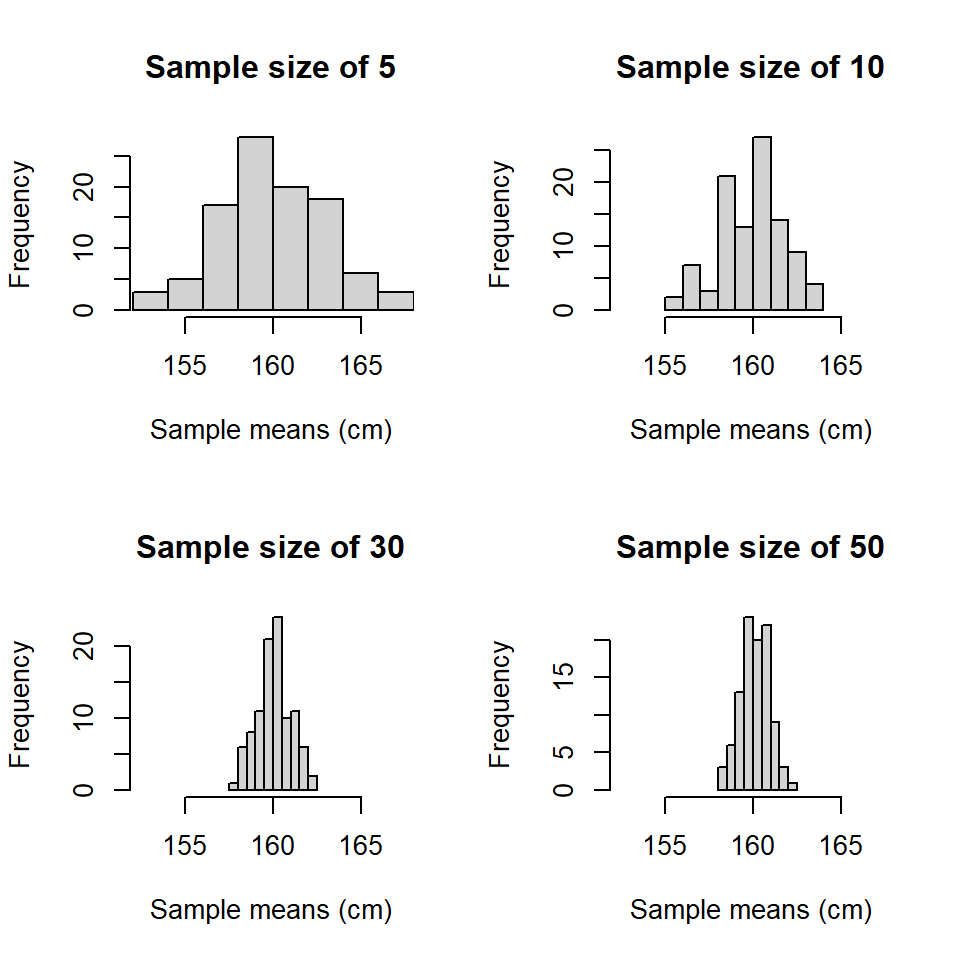
\includegraphics{IntroStats_files/figure-latex/histsampsize-1} 

}

\caption{Distributions of 1000 sample means using four different sizes of sample. The underlying population was $N(160,6^2)$.}\label{fig:histsampsize}
\end{figure}

There are two things to notice about these distributions of sample means:

\begin{itemize}
\tightlist
\item
  the distributions are centered about the true population mean of 160,
  and
\item
  the sample means range from about 152 to 168 when the sample size is 5, but this spread reduces as the sample size increases.
\end{itemize}

These patterns will be similar for any distribution of sample estimates and so can be used to inform how precise a sample mean might be.

\hypertarget{precision-of-the-sample-mean}{%
\subsection{Precision of the sample mean}\label{precision-of-the-sample-mean}}

The standard deviation of the sample means is found by dividing the population standard deviation by the square root of the sample size being averaged:

\[sd(\textrm{sample mean}) = \frac{\textrm{Population SD}}{\sqrt{\textrm{sample size}}}\]

The standard deviation of a sampling distribution is called a \textbf{standard error}. Therefore, substituting the usual notation (see Chapter \ref{describedata}) into this formula, the standard error of the mean is given by:

\[se(\hat \mu) = \frac{\sigma}{\sqrt{n}}\]

Thus, using the height data, the standard error for a sample size of 5 is given by:

\[se(\hat \mu) = \frac{6}{\sqrt{5}} = 2.68\]

As shown in Figure \ref{fig:histsampsize}, the standard deviation (and hence standard error) of the distribution of the sample mean reduces as the sample size increases; the standard error using a sample size of 30 is

\[se(\hat \mu) = \frac{6}{\sqrt{30}} = 1.095\]

\hypertarget{confidence-interval-with-known-sigma}{%
\subsection{\texorpdfstring{Confidence interval with known \(\sigma\)}{Confidence interval with known \textbackslash sigma}}\label{confidence-interval-with-known-sigma}}

In this example, we assumed the data were normally distributed and, as we have seen in Figure \ref{fig:histsampsize}, the distributions of the sample mean were also normally distributed. This is very handy because we know that for any normally distributed variable, 95\% of the time a randomly chosen value will fall within 1.96 standard deviations of the mean. Hence, the sample mean will fall within 1.96 standard deviations of the true population mean about 95\% of the time (or for about 95\% of samples taken). While we rarely know the true population mean, it is likely that the estimate of the sample mean will fall within about 1.96 standard deviations of the population mean. Thus, we can derive an upper and lower limit between which we think the true population mean will lie - this is called a confidence interval. A 95\% confidence interval for the sample mean is given by the following:

\[ \hat \mu - 1.96 \times \frac{\sigma}{\sqrt{n}} \quad ; \quad \hat \mu + 1.96 \times \frac{\sigma}{\sqrt{n}}\]
or, writing this more succinctly as,

\[ \hat \mu \pm 1.96 \times \frac{\sigma}{\sqrt{n}}\]

Thus, for a sample of size 5, the 95\% confidence interval for the mean will be

\[157.9 \pm 1.96 \times 2.68\]

\[157.9 \pm 5.25\]

which results in the limits 152.6 cm and 163.2 cm. We can see for a distribution with a mean and variance equal to our sample mean and standard deviation i.e.~\(N(\mu=157.9, \sigma^2=2.68^2)\), that 95\% of the distribution lies between these limits (Figure \ref{fig:popci}). This means that if we repeatedly take samples of size 5, calculate the sample mean and a 95\% CI for the mean, 95\% of the confidence intervals will include the true population mean.

\begin{figure}

{\centering 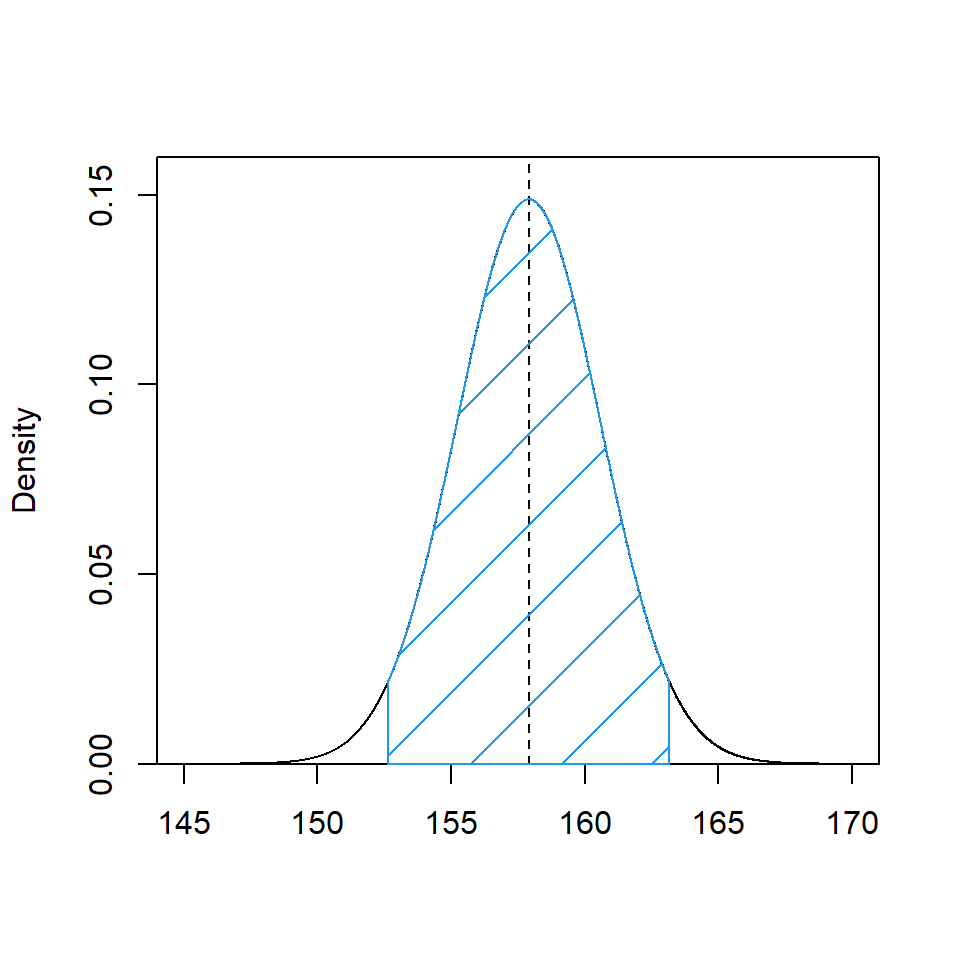
\includegraphics{IntroStats_files/figure-latex/popci-1} 

}

\caption{Sampling distribution of the sample mean for a sample of size 5. 95\% of the central part of the distribution is shaded blue. The sample mean is shown by the dotted line.}\label{fig:popci}
\end{figure}

We can think of 1.96 as a value which multiplies the standard error to provide a value above and below the sample mean to create the confidence interval. Increasing or decreasing this multiplier will result in wider and narrower intervals and we look at this later. Before that we consider a fundamental theorem in statistics.

To illustrate a confidence interval we used data from a normal distribution and, in general, we don't usually know if the data are drawn from a normal distribution! However, help is at hand in the form of the Central Limit Theorem.

\hypertarget{central-limit-theorem}{%
\subsubsection{Central limit theorem}\label{central-limit-theorem}}

The Central Limit Theorem (CLT) states that no matter what distribution we sample from, the \textbf{distribution of the sample means} (\(\hat \mu\)) is closely approximated by the normal distribution in large samples.

We can see this in Figure \ref{fig:histsampsize}, but how large a sample is required for reliable estimation of the population mean? The sample size required depends somewhat on the data: for data from symmetrical distributions a sample of 5 may be sufficient; for heavily skewed data a sample of 50 may be required.

In calculating a CI, we also need to consider the variability in the data and this is quantified by the standard deviation. In the example above, we knew the population standard deviation but what happens if we don't know the population standard deviation? We consider this next.

\hypertarget{confidence-interval-with-unknown-sigma}{%
\subsection{\texorpdfstring{Confidence interval with unknown \(\sigma\)}{Confidence interval with unknown \textbackslash sigma}}\label{confidence-interval-with-unknown-sigma}}

If the population standard deviation is unknown (and in fact the population standard deviation is rarely known), the population standard deviation (\(\sigma\)) is simply replaced by the sample standard deviation (\(s\)) in the formula for the standard error:

\[se(\hat \mu)=\frac{\textrm{sample SD}}{\sqrt{\textrm{sample size}}} = \frac{s}{\sqrt{n}}\]

Thus, for the sample of five heights, the sample standard deviation is 8.415 and so the sample standard error is

\[se(\hat \mu) = \frac{8.415}{\sqrt{5}} = 3.763\]

When we sample data from a normal distribution and we know the population standard deviation (\(\sigma\)), the distribution of sample means is exactly normally distributed about the true population mean, \(\mu\). When we don't know the population standard deviation, we introduce a new source of variability because we use the sample standard deviation of the data instead of a known population standard deviation. Therefore, rather than using quantiles from the normal distribution to find the multipliers needed to calculate the confidence interval, we use a different distribution; the \(t\) distribution is used to find the multiplier. Before continuing with the calculation we look at the \(t\) distribution and see how it compares to a standard normal distribution.

\hypertarget{the-t-distribution}{%
\subsubsection{\texorpdfstring{The \(t\) distribution}{The t distribution}}\label{the-t-distribution}}

The \(t\) distribution (also known as Student's \(t\) distribution) is symmetrical about zero and has a similar shape to the standard normal distribution. However, rather than being defined by a mean and variance, the \(t\) distribution is indexed by a parameter called the degrees of freedom (\(df\)) (i.e.~\(t_{df}\)). The degrees of freedom are determined by the sample size such that \(df=n-1\). When \(n\) is small the \(t\) distribution has fatter tails and a flatter top compared with the normal distribution; as \(n\) (and thus \(df\)) increases, the \(t\) distribution become more and more like a standard normal distribution (Figure \ref{fig:tandnormplot}). As an example, when \(n=11\), and hence \(t_{df=10}\), only 92\% of the distribution falls within 1.96 standard deviations either side the mean, whereas for a standard normal distribution, 95\% of the distribution falls within 1.96 standard deviations of the mean. For a \(t_{df=10}\) distribution, 95\% of the distribution will lie between 2.23 standard deviations of the mean.

\begin{figure}[!htb]

{\centering 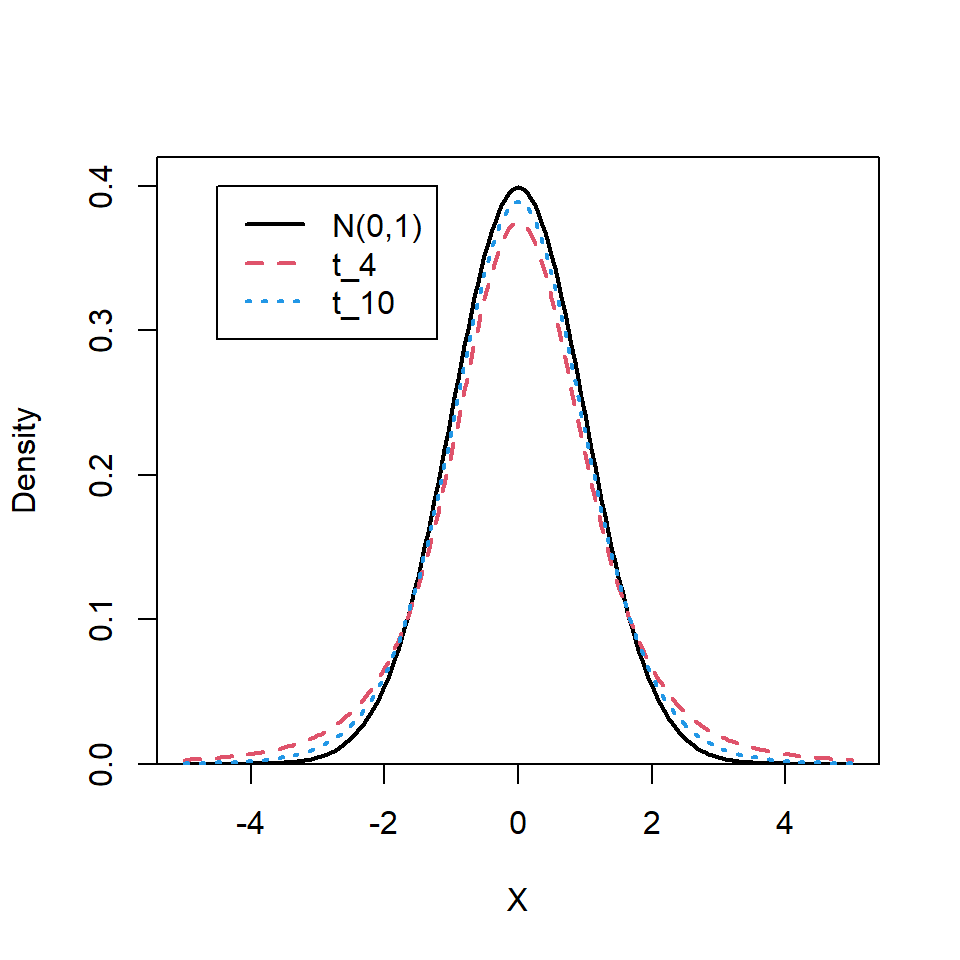
\includegraphics{IntroStats_files/figure-latex/tandnormplot-1} 

}

\caption{Comparison of standard normal and $t$ distributions with 4 and 10 $df$.}\label{fig:tandnormplot}
\end{figure}

\hypertarget{confidence-interval-for-the-sample-mean}{%
\subsubsection{Confidence interval for the sample mean}\label{confidence-interval-for-the-sample-mean}}

When the population standard deviation is unknown and estimated by the sample standard deviation, the multiplier is found from the \(t\) distribution such that the confidence interval limits are found from

\[\hat{\mu} - t_{(1-(\alpha/2), df=n-1)} \times \frac{s}{\sqrt{n}} \quad;\quad \hat{\mu} + t_{(1-(\alpha/2), df=n-1)} \times \frac{s}{\sqrt{n}}\]
or more succinctly,

\[\hat{\mu}\pm t_{(1-(\alpha/2), df=n-1)}se(\hat{\mu})\]

where \(t_{(1-\alpha/2, df=n-1)}\) represents a value (multiplier) from the \(t_{df=(n-1)}\) distribution; this indicates how far we need to extend either side of the sample estimate in order to `catch' the true mean with some associated confidence, represented by \(\alpha\). The confidence represents how confident we want to be that the interval contains the true mean.

The most frequently quoted CI are 95\% confidence intervals (i.e.~we want to be 95\% confident that the interval contains the true mean). For 95\% CI, \(\alpha = 5\)\%, thus \(1 - \frac{\alpha}{2} = 1 - \frac{0.05}{2} = 0.975\). Thus, the multiplier is the quantile \(q\) such that \(Pr(X \le q) = 0.975\) where \(X \sim t_{{df}}\).

To illustrate how to find the multiplier, let's return to the height sample data. Figure @ref(fig:tdist.ca) shows that a \(Pr(X \le 2.78) = 0.975\) and because the \(t\) distribution is symmetric round zero, we know that \(Pr(X \le -2.78) = 0.025\), hence 95\% of the area (the red shaded area) will lie between -2.78 and 2.78 where \(df=4\).

(ref:tdist.ca) Probability density distribution for \(t_{df=4}\). The red shaded area is 95\% of the area with 2.5\% in each tail.

\begin{figure}[!htb]

{\centering 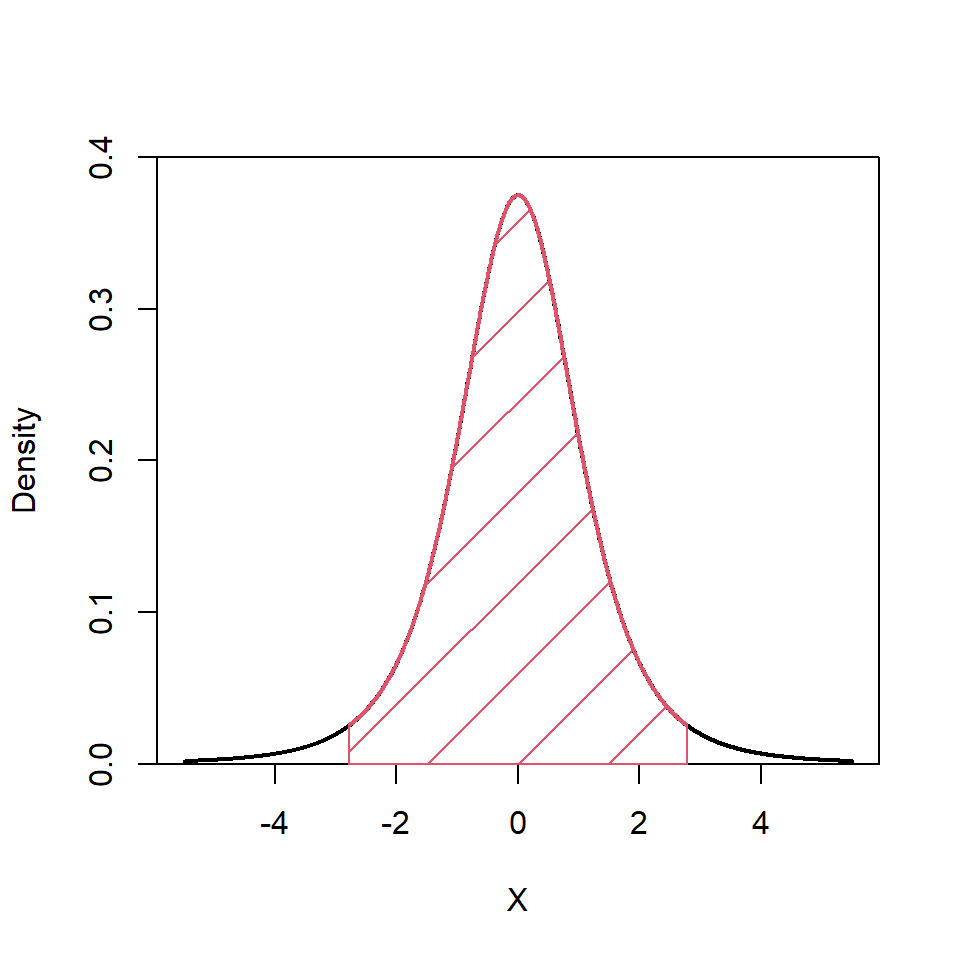
\includegraphics{IntroStats_files/figure-latex/tdist.ca-1} 

}

\caption{(ref:tdist.ca)}(\#fig:tdist.ca)
\end{figure}

Thus using the sample standard deviation, the interval is found from:

\[157.9 \pm t_{0.975, \textrm{df}=4} \times 3.763\]

and substituting in the value for the \(t\)-multiplier, \(t_{0.975, \textrm{df}=4} = 2.78\), gives

\[157.9 \pm 2.78 \times 3.763\]
\[157.9 \pm 10.46\]

Thus, the 95\% confidence interval for the mean is 147.4 to 168.4 cm; 95\% of the time the true mean will lie in the range 147.4 and 168.4 cm. This is wider than the confidence interval found using the population standard deviation (which was 152.6 to 163.2 cm) because of the additional uncertainty about the variability of the distribution.

\hypertarget{what-does-confidence-mean}{%
\subsubsection{What does confidence mean?}\label{what-does-confidence-mean}}

Confidence is a long run process, it does not apply to any one particular interval. Essentially, if we repeatedly take samples from a population and calculate a 95\% CI (just as we have done above for one sample), 95\% of the intervals will contain the true population mean. That means 5\% of the intervals will not contain the true mean!

If we wanted to increase the chance of catching the true mean, the interval could be widened by considering 99\% confidence intervals. In this case for our sample of five heights, the \(t\)-multiplier would be 4.6 resulting in an interval of 140.6 to 175.2 cm. Conversely, a 90\% confidence interval would be narrower i.e.~(149.9 to 165.9 cm). Both 90\% and 99\% confidence intervals are used but 95\% CI are the ones most frequently stated.

\hypertarget{doing-this-in-r-7}{%
\subsubsection{Doing this in R}\label{doing-this-in-r-7}}

To start with, we illustrate how to calculate a confidence interval by obtaining all the individual components. The \(t\)-multiplier is found from the cumulative distribution function for the \(t\) distribution \texttt{qt} - this is similar to the \texttt{qnorm} function introduced in Chapter \ref{contrv}.

\begin{Shaded}
\begin{Highlighting}[]
\CommentTok{\# 95\% CI for the sample mean assuming underlying population is normal}

\CommentTok{\# Create object for sample data}
\NormalTok{hgt }\OtherTok{\textless{}{-}} \FunctionTok{c}\NormalTok{(}\FloatTok{152.7}\NormalTok{, }\FloatTok{161.7}\NormalTok{, }\FloatTok{166.6}\NormalTok{, }\FloatTok{145.9}\NormalTok{, }\FloatTok{162.6}\NormalTok{)}

\CommentTok{\# Save the individual components of the CI}
\CommentTok{\# Sample mean}
\NormalTok{mean.hgt }\OtherTok{\textless{}{-}} \FunctionTok{mean}\NormalTok{(hgt)}
\NormalTok{mean.hgt}
\end{Highlighting}
\end{Shaded}

\begin{verbatim}
[1] 157.9
\end{verbatim}

\begin{Shaded}
\begin{Highlighting}[]
\CommentTok{\# Sample standard deviation}
\NormalTok{sd.hgt }\OtherTok{\textless{}{-}} \FunctionTok{sd}\NormalTok{(hgt)}
\NormalTok{sd.hgt}
\end{Highlighting}
\end{Shaded}

\begin{verbatim}
[1] 8.415165
\end{verbatim}

\begin{Shaded}
\begin{Highlighting}[]
\CommentTok{\# Number of observations}
\NormalTok{n }\OtherTok{\textless{}{-}} \FunctionTok{length}\NormalTok{(hgt)}
\NormalTok{n}
\end{Highlighting}
\end{Shaded}

\begin{verbatim}
[1] 5
\end{verbatim}

\begin{Shaded}
\begin{Highlighting}[]
\CommentTok{\# Calculate standard error}
\NormalTok{se.hgt }\OtherTok{\textless{}{-}}\NormalTok{ sd.hgt}\SpecialCharTok{/}\FunctionTok{sqrt}\NormalTok{(n)}
\NormalTok{se.hgt}
\end{Highlighting}
\end{Shaded}

\begin{verbatim}
[1] 3.763376
\end{verbatim}

\begin{Shaded}
\begin{Highlighting}[]
\CommentTok{\# t{-}multiplier for 95\% CI}
\NormalTok{tmult }\OtherTok{\textless{}{-}} \FunctionTok{qt}\NormalTok{(}\AttributeTok{p=}\FloatTok{0.975}\NormalTok{, }\AttributeTok{df=}\DecValTok{4}\NormalTok{)}
\NormalTok{tmult}
\end{Highlighting}
\end{Shaded}

\begin{verbatim}
[1] 2.776445
\end{verbatim}

\begin{Shaded}
\begin{Highlighting}[]
\CommentTok{\# Lower limit}
\NormalTok{mean.hgt }\SpecialCharTok{{-}}\NormalTok{ (tmult}\SpecialCharTok{*}\NormalTok{se.hgt)}
\end{Highlighting}
\end{Shaded}

\begin{verbatim}
[1] 147.4512
\end{verbatim}

\begin{Shaded}
\begin{Highlighting}[]
\CommentTok{\# Upper limit}
\NormalTok{mean.hgt }\SpecialCharTok{+}\NormalTok{ (tmult}\SpecialCharTok{*}\NormalTok{se.hgt)}
\end{Highlighting}
\end{Shaded}

\begin{verbatim}
[1] 168.3488
\end{verbatim}

The above commands illustrate how to construct the confidence intervals from the individual components. However, there is a short cut (isn't there always in R) to obtain a CI. We make use of the \texttt{t.test} function; the \texttt{t.test} function does a lot more than provide confidence intervals (which we will explore in the following chapter) but for now we only want the CI which are given by specifying \texttt{\$conf.int}.

\begin{Shaded}
\begin{Highlighting}[]
\CommentTok{\# 95\% CI (default)}
\FunctionTok{t.test}\NormalTok{(}\AttributeTok{x=}\NormalTok{hgt)}\SpecialCharTok{$}\NormalTok{conf.int}
\end{Highlighting}
\end{Shaded}

\begin{verbatim}
[1] 147.4512 168.3488
attr(,"conf.level")
[1] 0.95
\end{verbatim}

\begin{Shaded}
\begin{Highlighting}[]
\CommentTok{\# 90\% CI}
\FunctionTok{t.test}\NormalTok{(}\AttributeTok{x=}\NormalTok{hgt, }\AttributeTok{conf.level=}\FloatTok{0.90}\NormalTok{)}\SpecialCharTok{$}\NormalTok{conf.int}
\end{Highlighting}
\end{Shaded}

\begin{verbatim}
[1] 149.8771 165.9229
attr(,"conf.level")
[1] 0.9
\end{verbatim}

\begin{Shaded}
\begin{Highlighting}[]
\CommentTok{\# 99\% CI}
\FunctionTok{t.test}\NormalTok{(}\AttributeTok{x=}\NormalTok{hgt, }\AttributeTok{conf.level=}\FloatTok{0.99}\NormalTok{)}\SpecialCharTok{$}\NormalTok{conf.int}
\end{Highlighting}
\end{Shaded}

\begin{verbatim}
[1] 140.5731 175.2269
attr(,"conf.level")
[1] 0.99
\end{verbatim}

\textbf{Q7.1} A researcher was interested in the typical size of trees (measured as diameter at breast height, dbh) of a particular species in a forest. Data on dbh (in cm) had been collected on a sample of 50 trees. The mean dbh was 765 cm and the standard deviation was 3.

\textbf{a.} What is the standard error of the mean?

\textbf{b.} Which of the following multipliers should be used for a 90\% confidence interval?

\begin{Shaded}
\begin{Highlighting}[]
\FunctionTok{qt}\NormalTok{(}\AttributeTok{p=}\FloatTok{0.90}\NormalTok{, }\AttributeTok{df=}\DecValTok{49}\NormalTok{)}
\end{Highlighting}
\end{Shaded}

\begin{verbatim}
[1] 1.299069
\end{verbatim}

\begin{Shaded}
\begin{Highlighting}[]
\FunctionTok{qnorm}\NormalTok{(}\FloatTok{0.05}\NormalTok{)}
\end{Highlighting}
\end{Shaded}

\begin{verbatim}
[1] -1.644854
\end{verbatim}

\begin{Shaded}
\begin{Highlighting}[]
\FunctionTok{qt}\NormalTok{(}\AttributeTok{p=}\FloatTok{0.95}\NormalTok{, }\AttributeTok{df=}\DecValTok{49}\NormalTok{)}
\end{Highlighting}
\end{Shaded}

\begin{verbatim}
[1] 1.676551
\end{verbatim}

\begin{Shaded}
\begin{Highlighting}[]
\FunctionTok{qt}\NormalTok{(}\AttributeTok{p=}\FloatTok{0.975}\NormalTok{, }\AttributeTok{df=}\DecValTok{49}\NormalTok{)}
\end{Highlighting}
\end{Shaded}

\begin{verbatim}
[1] 2.009575
\end{verbatim}

\textbf{c.} Calculate a 90\% confidence interval for the mean.

\textbf{d.} Interpret the confidence interval.

\textbf{Q7.2} A study of birth weight was conducted in San Francisco, US. The summary statistics of weights of babies for the group of non-smoking mothers are as follows: \(n=742\), \(\hat \mu = 123.05\) ounces and \(s = 17.4\) ounces. Calculate a 95\% confidence interval for the mean; the sample size is large and so assume that the \(t\) multiplier is 1.96. The full data set can be found \href{https://www.stat.berkeley.edu/users/statlabs/labs.html}{here}.

\hypertarget{difference-between-two-group-means}{%
\section{Difference between two group means}\label{difference-between-two-group-means}}

Sometimes we want to compare two means, for example the mean blood pressure of patients that have received one of two treatments or the mean yield of tomato plants grown in one of two varieties of potting compost. Hence, we are interested in the difference between the two means and want to find a confidence interval for the difference. The process is very similar to that described previously.

Assume we have two groups, which we call \(A\) and \(B\), and sample means have been obtained, \(\hat \mu_A\) and \(\hat \mu_B\). The difference between the sample means is simply given by

\[\textrm{difference } A - B = \hat \mu_A - \hat \mu_B\]

If this difference is zero (or very close to zero), then it likely that there is no real difference between these two groups. However, if it is not zero there are two possible alternatives:

\begin{itemize}
\tightlist
\item
  the two samples are from the same parent population and the difference is due to sampling variability, or
\item
  the two samples are from different populations and so there is a difference beyond any sampling variability.
\end{itemize}

The phrase `different populations' is used here to refer to parent populations that have different population means, however, we also need to consider whether the parent populations have different standard deviations; as we shall see, this is taken account of when considering the precision of the estimate of the difference.

In the next chapter we look at formal statistical tests to determine between the two alternatives described above but here we want to find an interval around the estimate of the difference that we are confident (to some level) contains the true difference.

The confidence interval for the difference in the means is given by:

\[(\hat \mu_A - \hat \mu_B) \pm t_{(1-(\alpha/2), n-1)}se(\hat \mu_A - \hat \mu_B)\]

where \(se(\hat \mu_A - \hat \mu_B)\) is the standard error of the difference.

The standard error of the difference is obtained by combining the uncertainty of the two sample estimates and the calculation depends on whether the variability of the two groups can be assumed to be the same (or very similar) or not.

\textbf{Q7.3} According to an advertising campaign, batteries from brand \(A\) last longer than
batteries from brand \(B\). In order to compare the two brands we select a random sample of 90 brand \(A\) batteries and 60 brand \(B\) batteries. The sample of brand \(A\) batteries run continuously for a total of 4451 minutes with a sample standard deviation of 6.32 minutes. The sample of brand \(B\) batteries run continuously for a total of 2763 minutes with a sample standard deviation of 3.31 minutes. Assume that the data are normally distributed.

Find estimates for \(\hat \mu_A\) and \(\hat \mu_B\), the mean running time of a battery from brand \(A\) and brand \(B\), respectively. Hence find an estimate for the difference in mean running time between the two brands.

\hypertarget{assuming-equal-standard-deviations-of-the-two-groups}{%
\subsection{Assuming equal standard deviations of the two groups}\label{assuming-equal-standard-deviations-of-the-two-groups}}

If we can assume that the two groups have the same variability, we pool the information on variability (quantified by the sample standard deviations) to generate an estimate of the pooled variability.

The standard error of the difference in sample means is the pooled estimate of the common standard deviation (\(s_p\)) (assuming that the variances in the populations are similar) computed as the weighted average of the standard deviations in the samples,

\[se(\hat{\mu_A} - \hat{\mu_B})=s_p\sqrt{\frac{1}{n_A} + \frac{1}{n_B}}\]

where \(s_p\) is the pooled standard deviation and is found as follows:

\[ s_p = \sqrt{\frac{(n_A-1)s_A^2 + (n_B-1)s_B^2}{n_A + n_B -2}}\]
The pooled degrees of freedom are given by \(df=(n_A + n_B - 2)\). These degrees of freedom are then used to find the multiplier \(t_{(1-(\alpha/2), df)}\).

This specification for the standard error and degrees of freedom are only appropriate when the two groups have equal standard deviations.

\textbf{Example} We continue to look at data collected from the observational study of birth weights introduced in Q7.1. In total, 1236 women were enrolled in the study and the participants came from a wide range of economic, social and educational backgrounds. We want to calculate a 95\% confidence interval for the difference between the means for the mothers who smoked and mothers who did not smoke. The summary data are provided in Table \ref{tab:babywgttab}.

\begin{longtable}[]{@{}cccc@{}}
\caption{\label{tab:babywgttab} Summary of birth weight data for the smoking and non-smoking groups (units are ounces); n is sample size and SD is the standard deviation.}\tabularnewline
\toprule
\begin{minipage}[b]{(\columnwidth - 3\tabcolsep) * \real{0.14}}\centering
Smoking\strut
\end{minipage} & \begin{minipage}[b]{(\columnwidth - 3\tabcolsep) * \real{0.08}}\centering
n\strut
\end{minipage} & \begin{minipage}[b]{(\columnwidth - 3\tabcolsep) * \real{0.12}}\centering
Mean\strut
\end{minipage} & \begin{minipage}[b]{(\columnwidth - 3\tabcolsep) * \real{0.12}}\centering
SD\strut
\end{minipage}\tabularnewline
\midrule
\endfirsthead
\toprule
\begin{minipage}[b]{(\columnwidth - 3\tabcolsep) * \real{0.14}}\centering
Smoking\strut
\end{minipage} & \begin{minipage}[b]{(\columnwidth - 3\tabcolsep) * \real{0.08}}\centering
n\strut
\end{minipage} & \begin{minipage}[b]{(\columnwidth - 3\tabcolsep) * \real{0.12}}\centering
Mean\strut
\end{minipage} & \begin{minipage}[b]{(\columnwidth - 3\tabcolsep) * \real{0.12}}\centering
SD\strut
\end{minipage}\tabularnewline
\midrule
\endhead
\begin{minipage}[t]{(\columnwidth - 3\tabcolsep) * \real{0.14}}\centering
No\strut
\end{minipage} & \begin{minipage}[t]{(\columnwidth - 3\tabcolsep) * \real{0.08}}\centering
742\strut
\end{minipage} & \begin{minipage}[t]{(\columnwidth - 3\tabcolsep) * \real{0.12}}\centering
123.05\strut
\end{minipage} & \begin{minipage}[t]{(\columnwidth - 3\tabcolsep) * \real{0.12}}\centering
17.4\strut
\end{minipage}\tabularnewline
\begin{minipage}[t]{(\columnwidth - 3\tabcolsep) * \real{0.14}}\centering
Yes\strut
\end{minipage} & \begin{minipage}[t]{(\columnwidth - 3\tabcolsep) * \real{0.08}}\centering
484\strut
\end{minipage} & \begin{minipage}[t]{(\columnwidth - 3\tabcolsep) * \real{0.12}}\centering
114.11\strut
\end{minipage} & \begin{minipage}[t]{(\columnwidth - 3\tabcolsep) * \real{0.12}}\centering
18.1\strut
\end{minipage}\tabularnewline
\bottomrule
\end{longtable}

The estimate for the difference between the non-smoking group (\(N\)) and the smoking group (\(S\)) is given by

\[\hat \mu_N - \hat \mu_S = 123.05 - 114.11  = 8.94\]

In this example, the sample standard deviations are very similar and so we will calculate the pooled standard deviation:

\[ s_p = \sqrt{\frac{(n_N-1)s_N^2 + (n_S-1)s_S^2}{n_N + n_S -2}}\]
Substituting in the values gives:

\[ s_p = \sqrt{\frac{(742-1)17.4^2 + (484-1)18.1^2}{742 + 484 -2}}  = \sqrt{\frac{382580.8}{1224}} = 17.68\]
Thus, the standard error is

\[se(\hat{\mu}_N - \hat{\mu}_S)=s_p\sqrt{\frac{1}{n_N} + \frac{1}{n_S}} = 17.68 \sqrt{\frac{1}{742} + \frac{1}{484}} = 1.033\]

The degrees of freedom are

\[df = 742 + 484 - 2 = 1224\]

The next component of the confidence interval is the multiplier \(t_{(1-\frac{\alpha}{2}, df)}\). For a 95\% confidence interval, \(\alpha=0.05\) and so we want the quantile associated with \(t_{(0.975,df=1224)}\). The degrees of freedom are large and so the relevant \(t\) distribution will be very similar to the normal distribution; the actual value of the multiplier is 1.9619. Thus the 95\% confidence interval is given by

\[8.94 \pm 1.9619 \times 1.033 \]

\[8.94 \pm 2.027\]

which results in an interval 6.91 to 10.97 ounces. This interval indicates that we can be 95\% confident that, on average, a baby with a non-smoking mother is likely to be about 7 to 11 ounces heavier than a baby with a mother who smokes.

\hypertarget{doing-this-in-r-8}{%
\subsubsection{Doing this in R}\label{doing-this-in-r-8}}

Again we can call on the \texttt{t.test} function to calculate a CI for the difference between two sample means. In the code below, the birth weights for non-smokers and smokers have been stored in objects called \texttt{grpN} and \texttt{grpS}, respectively.

\begin{Shaded}
\begin{Highlighting}[]
\CommentTok{\# 95\% CI}
\FunctionTok{t.test}\NormalTok{(}\AttributeTok{x=}\NormalTok{grpN, }\AttributeTok{y=}\NormalTok{grpS, }\AttributeTok{var.equal=}\ConstantTok{TRUE}\NormalTok{)}\SpecialCharTok{$}\NormalTok{conf.int}
\end{Highlighting}
\end{Shaded}

\begin{verbatim}
[1]  6.911199 10.964133
attr(,"conf.level")
[1] 0.95
\end{verbatim}

\textbf{Q7.4} For the details of battery running times provided in Q7.3, calculate the standard error (assuming the standard deviations are equal) for the difference in mean running time and hence, using the following information, calculate a 95\% confidence interval for the difference in means.

\begin{Shaded}
\begin{Highlighting}[]
\FunctionTok{qt}\NormalTok{(}\AttributeTok{p=}\FloatTok{0.975}\NormalTok{, }\AttributeTok{df=}\DecValTok{148}\NormalTok{)}
\end{Highlighting}
\end{Shaded}

\begin{verbatim}
[1] 1.976122
\end{verbatim}

\hypertarget{assuming-unequal-standard-deviations-of-the-two-groups}{%
\subsection{Assuming unequal standard deviations of the two groups}\label{assuming-unequal-standard-deviations-of-the-two-groups}}

If the standard deviations of the two groups cannot be assumed to be equal, then to accurately describe the differences we need to alter the standard error and degrees of freedom calculations. This standard error formula is:

\[se(\hat{\mu}_A - \hat{\mu}_B)= \sqrt{\frac{{s_A}^2}{{n_A}} + \frac{{s_B}^2}{{n_B}}}\]

To calculate the degrees of freedom when doing the calculation by hand, use the minimum value out of \(n_A-1\) and \(n_B -1\):

\[df = Min(n_A-1, n_B -1)\]

In computing packages, the more exact (but also more tricky to calculate by hand) Welch-Satterthwaite equation is used:

\[df_w = \frac{\left(\frac{s_A^2}{n_A} + \frac{s_B^2}{n_B}\right)^2}{\frac{s_A^4}{n_A^2(n_A-1)} + \frac{s_A^4}{n_A^2(n_A-1)}}\]

The Welch-Satterthwaite approximation for df (\(df_w\)) is always smaller than the degrees of freedom under equal standard deviation, so for the same \(\alpha\) level, the multiplier will be wider. We will investigate the effects of using this more exact formula further in the computer practical associated with this chapter.

\textbf{Example} Using the summary data in Table \ref{tab:babywgttab}, we calculate the 95\% confidence interval for the difference in means using the standard error formula that should be used if we cannot assume that the standard deviations of the two groups are the same.

The standard error formula, assuming that the standard deviations of the two groups are not equal is:

\[se(\hat{\mu}_N - \hat{\mu}_S)= \sqrt{\frac{{s_N}^2}{{n_N}} + \frac{{s_S}^2}{{n_S}}} = \sqrt{\frac{17.4^2}{742} + \frac{18.1^2}{484}} = 1.04\]

Since we are doing this calculation by hand the following formula is used to obtain the degrees of freedom.

\[df = Min(742-1, 484-1) = 483\]
This results in a multiplier of 1.965, thus, the 95\% confidence is given by

\[8.94 \pm 1.965 \times 1.04\]
which results in an interval (6.90, 10.98), hence we can be 95\% confident that the difference in birth weights between the smoking and non-smoking mothers is between 6.9 and 11 ounces.

This is generally the approach that should be used to obtain the confidence interval because the previous approach should only be used if it can be assumed that the population standard deviations (which we generally don't know) are equal.

\hypertarget{doing-this-in-r-9}{%
\subsubsection{Doing this in R}\label{doing-this-in-r-9}}

The assumption that the standard deviations are unequal is specified by default (with the \texttt{var.equal=FALSE}) but it is useful to include this argument for clarity.

\begin{Shaded}
\begin{Highlighting}[]
\CommentTok{\# 95\% CI}
\FunctionTok{t.test}\NormalTok{(}\AttributeTok{x=}\NormalTok{grpN, }\AttributeTok{y=}\NormalTok{grpS, }\AttributeTok{var.equal=}\ConstantTok{FALSE}\NormalTok{)}\SpecialCharTok{$}\NormalTok{conf.int}
\end{Highlighting}
\end{Shaded}

\begin{verbatim}
[1]  6.89385 10.98148
attr(,"conf.level")
[1] 0.95
\end{verbatim}

\textbf{Q7.5} Using the information in Q7.3, calculate the standard error for the difference in mean running times assuming that the standard deviations are not equal and hence calculate the 95\% confidence interval. Calculate the degrees of freedom and select the correct multiplier from the following information.

\begin{Shaded}
\begin{Highlighting}[]
\FunctionTok{qt}\NormalTok{(}\FloatTok{0.975}\NormalTok{, }\AttributeTok{df=}\DecValTok{59}\NormalTok{)}
\end{Highlighting}
\end{Shaded}

\begin{verbatim}
[1] 2.000995
\end{verbatim}

\begin{Shaded}
\begin{Highlighting}[]
\FunctionTok{qt}\NormalTok{(}\FloatTok{0.975}\NormalTok{, }\AttributeTok{df=}\DecValTok{148}\NormalTok{)}
\end{Highlighting}
\end{Shaded}

\begin{verbatim}
[1] 1.976122
\end{verbatim}

\hypertarget{empirical-bootstrap-based-confidence-intervals}{%
\section{Empirical (bootstrap-based) confidence intervals}\label{empirical-bootstrap-based-confidence-intervals}}

In the calculation of confidence intervals so far we have relied on the CLT. In some circumstances, for example if the sample size is very small or the wider (or parent) population is very skewed, we may not be able to safely assume that the distribution of the sample mean is approximately normal. In such cases, the confidence interval may not capture the true parameter with the required level of confidence and so an alternative method for calculating confidence intervals may be more appropriate. An \textbf{empirical} (also called \textbf{non-parametric} or \textbf{bootstrap}) approach is a useful alternative to obtaining a confidence interval.

Assume we want to obtain a CI for a sample mean, then the empirical, bootstrap approach is as follows:

\begin{enumerate}
\def\labelenumi{\arabic{enumi}.}
\item
  Select \(n\) values at random and \textbf{with replacement} from our original sample of \(n\) values.

  \begin{itemize}
  \tightlist
  \item
    If we have 100 values in the original sample, we randomly select a sample of 100 values.
  \item
    Sampling with replacement, means some of the observations in the original data may be selected several times and other observations not selected at all.
  \end{itemize}
\item
  Calculate the mean for this generated sample.
\item
  Repeat steps 1 and 2 many times (e.g.~at least 1000 times).

  \begin{itemize}
  \tightlist
  \item
    For example, if we took 1000 samples each with \(n=100\), this would give us a set of 1000 mean values.
  \end{itemize}
\item
  Examine the distribution of these sample estimates and locate the values which define the central 95\% of the values in this distribution (whatever it's shape) (i.e.~the 2.5 and 97.5 percentiles).

  \begin{itemize}
  \tightlist
  \item
    These are called `percentile' confidence intervals.
  \end{itemize}
\end{enumerate}

This method has the advantage that,

\begin{itemize}
\tightlist
\item
  it side-steps the assumption that the distribution of sample estimates is normally distributed and simply locates the central 95\% of the sample estimates.
\item
  it can be used to obtain confidence intervals for the median or a difference between means, or any other statistic of interest.
\end{itemize}

However,

\begin{itemize}
\tightlist
\item
  this approach can be computationally intensive,
\item
  and because of the random nature it may not always provide the desired coverage (e.g.~the intervals may be too small or too large and may not capture the parameter of interest with the desired confidence).
\end{itemize}

To illustrate this approach we will use it to find a confidence interval for the mean weights of babies described in Q7.1. To discover more about the bootstrap then see \citep{Davison1997}.

\hypertarget{doing-this-in-r-10}{%
\subsubsection{Doing this in R}\label{doing-this-in-r-10}}

The code below shows the steps involved to generate a bootstrap-based confidence interval for the mean weights of babies born to non-smoking mothers. The numbers relate to the steps outlined above. The weights are stored in an object called \texttt{grpN}.

To repeatedly perform the same commands a `\texttt{for} loop' is used to generate samples and calculate the sample mean; the commands within \texttt{\{\}} are repeated \texttt{B} times with the index \texttt{i} starting at 1 and increasing by 1 each time the loop is repeated.

\begin{Shaded}
\begin{Highlighting}[]
\CommentTok{\# R code to obtain a bootstrap confidence intervals for density}

\CommentTok{\# Number of bootstraps}
\NormalTok{B }\OtherTok{\textless{}{-}} \DecValTok{1000}
\CommentTok{\# Number of observations}
\NormalTok{n }\OtherTok{\textless{}{-}} \FunctionTok{length}\NormalTok{(grpN)}
\CommentTok{\# Create object to store bootstrap sample means}
\NormalTok{res1 }\OtherTok{\textless{}{-}} \FunctionTok{rep}\NormalTok{(}\ConstantTok{NA}\NormalTok{, B)}
\CommentTok{\# 3. Bootstrap loops}
\ControlFlowTok{for}\NormalTok{ (i }\ControlFlowTok{in} \DecValTok{1}\SpecialCharTok{:}\NormalTok{B) \{}
  \CommentTok{\# 1. Generate random sample from data with replacement}
\NormalTok{  bootsamp }\OtherTok{\textless{}{-}} \FunctionTok{sample}\NormalTok{(}\AttributeTok{x=}\NormalTok{grpN, }\AttributeTok{size=}\NormalTok{n, }\AttributeTok{replace=}\ConstantTok{TRUE}\NormalTok{)}
  \CommentTok{\# 2. Calculate mean of bootstrap sample and store}
\NormalTok{  res1[i] }\OtherTok{\textless{}{-}} \FunctionTok{mean}\NormalTok{(bootsamp) }
\NormalTok{\}}
\CommentTok{\# 4. Obtain central 95 percentiles for CI}
\FunctionTok{quantile}\NormalTok{(res1, }\AttributeTok{probs=}\FunctionTok{c}\NormalTok{(}\FloatTok{0.025}\NormalTok{, }\FloatTok{0.975}\NormalTok{))}
\end{Highlighting}
\end{Shaded}

\begin{verbatim}
    2.5%    97.5% 
121.7339 124.2144 
\end{verbatim}

\textbf{Creating a function}

If a series of commands are being used repeatedly (as in steps 1 and 2 in the code above), it often makes sense to combine them into a function. This is done in the code below.

\begin{Shaded}
\begin{Highlighting}[]
\NormalTok{samplemean.f }\OtherTok{\textless{}{-}} \ControlFlowTok{function}\NormalTok{(}\AttributeTok{sampdata=}\NormalTok{data, }\AttributeTok{do.replace=}\ConstantTok{TRUE}\NormalTok{) \{ }
  \CommentTok{\# Function to generate a sample and calculate the mean}
  \CommentTok{\# Arguments: }
    \CommentTok{\# sampdata = original sample }
    \CommentTok{\# do.replace = indicates whether sampling is with replacement, or not}
\NormalTok{  n }\OtherTok{\textless{}{-}} \FunctionTok{length}\NormalTok{(sampdata)}
\NormalTok{  bootsamp }\OtherTok{\textless{}{-}} \FunctionTok{sample}\NormalTok{(}\AttributeTok{x=}\NormalTok{sampdata, }\AttributeTok{size=}\NormalTok{n, }\AttributeTok{replace=}\NormalTok{do.replace)}
\NormalTok{  bootmean }\OtherTok{\textless{}{-}} \FunctionTok{mean}\NormalTok{(bootsamp)}
  \CommentTok{\# Return mean}
\NormalTok{  bootmean}
\NormalTok{\}}
\end{Highlighting}
\end{Shaded}

Defining a function follows certain conventions:

\begin{itemize}
\tightlist
\item
  the first line assigns the function contained in the function to a name (in this case \texttt{samplemean.f})
\item
  all arguments required for the function are specified at the top, including any default values,
\item
  all function commands are within the parentheses \texttt{\{\}}
\item
  the last line returns the result of the function.
\end{itemize}

Having created this function, we can amend the bootstrap code to include it:

\begin{Shaded}
\begin{Highlighting}[]
\CommentTok{\# Number of bootstraps}
\NormalTok{B }\OtherTok{\textless{}{-}} \DecValTok{1000}
\CommentTok{\# Create object to store sample means}
\NormalTok{res1 }\OtherTok{\textless{}{-}} \FunctionTok{rep}\NormalTok{(}\ConstantTok{NA}\NormalTok{, B)}
\CommentTok{\# 3. Bootstrap loops}
\ControlFlowTok{for}\NormalTok{ (i }\ControlFlowTok{in} \DecValTok{1}\SpecialCharTok{:}\NormalTok{B) \{}
  \CommentTok{\# 1. and 2. Obtain sample means with function}
\NormalTok{  res1[i] }\OtherTok{\textless{}{-}} \FunctionTok{samplemean.f}\NormalTok{(}\AttributeTok{sampdata=}\NormalTok{grpN, }\AttributeTok{do.replace=}\ConstantTok{TRUE}\NormalTok{)}
\NormalTok{\}}
\CommentTok{\# 4. Obtain 95 percentiles for CI}
\FunctionTok{quantile}\NormalTok{(res1, }\AttributeTok{probs=}\FunctionTok{c}\NormalTok{(}\FloatTok{0.025}\NormalTok{, }\FloatTok{0.975}\NormalTok{))}
\end{Highlighting}
\end{Shaded}

\begin{verbatim}
    2.5%    97.5% 
121.7559 124.2779 
\end{verbatim}

How does this empirical CI compare to that using the conventional method? The CIs obtained from the two methods should be similar; the sample size is fairly large and the heights are approximately normally distributed.

\textbf{Bootstrapping the easy way!}

The commands above have been included to illustrate all the steps in a bootstrap approach. However, in practice we don't need to write the code to perform such a bootstrap (unless you want to) because R contains a suite of functions which perform these commands; these require two additional libraries to be installed and then loaded into the R workspace with the \texttt{library} function.

The process requires two stages; one to generate the distribution of sample estimates and the second to obtain the confidence interval from the distribution.

The code below generates a CI for mean weight of babies from non-smoking mothers. The \texttt{oneboot} function generates the sample estimates and requires 3 arguments to be specified:

\begin{itemize}
\tightlist
\item
  \texttt{data} - the data to be bootstrapped, in this example, the weights are stored in an object called \texttt{grpN},
\item
  \texttt{FUN} - the name of the function used to calculate the statistic of interest (in this case, we want the \texttt{mean} but the \texttt{median} or \texttt{sd}, for example, could also be used), and
\item
  \texttt{R} - the number of repetitions.
\end{itemize}

The \texttt{boot.ci} function calculates the CI with the specified level of confidence.

\begin{Shaded}
\begin{Highlighting}[]
\CommentTok{\# Bootstrapping CI using built{-}in functions}

\CommentTok{\# Generate bootstrap sample means}
\FunctionTok{library}\NormalTok{(simpleboot)}
\NormalTok{bsmeans }\OtherTok{\textless{}{-}} \FunctionTok{one.boot}\NormalTok{(}\AttributeTok{data=}\NormalTok{grpN, }\AttributeTok{FUN=}\NormalTok{mean, }\AttributeTok{R=}\DecValTok{1000}\NormalTok{)}

\CommentTok{\# Obtain CI}
\FunctionTok{library}\NormalTok{(boot)}
\FunctionTok{boot.ci}\NormalTok{(bsmeans, }\AttributeTok{conf=}\FloatTok{0.95}\NormalTok{, }\AttributeTok{type=}\StringTok{"perc"}\NormalTok{) }
\end{Highlighting}
\end{Shaded}

\begin{verbatim}
BOOTSTRAP CONFIDENCE INTERVAL CALCULATIONS
Based on 1000 bootstrap replicates

CALL : 
boot.ci(boot.out = bsmeans, conf = 0.95, type = "perc")

Intervals : 
Level     Percentile     
95%   (121.8, 124.3 )  
Calculations and Intervals on Original Scale
\end{verbatim}

The CI is similar to those calculated previously but due to the random selection of data, the results from a bootstrap may be slightly different each time the code is executed.

The code below generates a CI for difference in mean weight of babies from non-smoking and smoking mothers using the \texttt{two.boot} function. The arguments are:

\begin{itemize}
\tightlist
\item
  \texttt{sample1} and \texttt{sample2} - the two groups of data, in this example, the weights are stored in objects called \texttt{grpN} and \texttt{grpS},
\item
  \texttt{FUN} - the name of the function used to calculate the statistic of interest (in this case, we want the difference between the means), and
\item
  \texttt{R} - the number of repetitions.
\end{itemize}

\begin{Shaded}
\begin{Highlighting}[]
\CommentTok{\# Bootstrapping CI using built{-}in functions}

\CommentTok{\# Generate bootstrap sample means}
\FunctionTok{library}\NormalTok{(simpleboot)}
\NormalTok{bsdiffs }\OtherTok{\textless{}{-}} \FunctionTok{two.boot}\NormalTok{(}\AttributeTok{sample1=}\NormalTok{grpN, }\AttributeTok{sample2=}\NormalTok{grpS, }\AttributeTok{FUN=}\NormalTok{mean, }\AttributeTok{R=}\DecValTok{1000}\NormalTok{)}

\CommentTok{\# Obtain CI}
\FunctionTok{library}\NormalTok{(boot)}
\FunctionTok{boot.ci}\NormalTok{(bsdiffs, }\AttributeTok{conf=}\FloatTok{0.95}\NormalTok{, }\AttributeTok{type=}\StringTok{"perc"}\NormalTok{) }
\end{Highlighting}
\end{Shaded}

\begin{verbatim}
BOOTSTRAP CONFIDENCE INTERVAL CALCULATIONS
Based on 1000 bootstrap replicates

CALL : 
boot.ci(boot.out = bsdiffs, conf = 0.95, type = "perc")

Intervals : 
Level     Percentile     
95%   ( 6.845, 10.975 )  
Calculations and Intervals on Original Scale
\end{verbatim}

\hypertarget{confidence-intervals-for-other-sample-statistics}{%
\section{Confidence intervals for other sample statistics}\label{confidence-intervals-for-other-sample-statistics}}

The methods described in this chapter can be adapted to find confidence intervals for other sample statistics, for example the median and variance. As previously mentioned, bootstrap confidence intervals can easily be obtained for these sample statistics in R by changing the \texttt{FUN} argument in the \texttt{one.boot} or \texttt{two.boot} functions.

Parametric confidence intervals can also be obtained in a similar manner to that of the sample mean. Rather than using the \(t\) distribution other statistical distributions are used; for example, for a CI for the variance a \(\chi^2\) distribution is used - this distribution is described in Chapter \ref{tableofcounts}.
A brief description of a CI for the median is given below. In a later chapter we look at confidence intervals for sample proportions.

\hypertarget{confidence-interval-for-the-median}{%
\subsubsection{Confidence interval for the median}\label{confidence-interval-for-the-median}}

For the median, the confidence interval is obtained slightly differently and because we are not making any assumptions about the distribution (e.g.~that it is symmetric), the CI is approximate.

Similar to the median, the CI is based on ranked values. The ranked value for the lower 95\% CI (for a sample of size \(n\)) is given by

\[\frac{n}{2} - \frac{1.96 \sqrt{n}}{2}\]
and the ranked value for the upper 95\% CI is given by

\[1 + \frac{n}{2} + \frac{1.96 \sqrt{n}}{2}\]

The CI is then obtained by finding the observed values associated with these ranked values.

\textbf{Example} The median weight of babies is 120 ounces. The sample size is 1236 and so the median was the average of the 618th and 619th ranked values. The ranked value for the lower 95\% CI is found from

\[\frac{1236}{2} - \frac{1.96 \sqrt{1236}}{2} = 618 - 34.45 = 583.55\]

The ranked value for the upper 95\% CI is found from

\[1 + \frac{1236}{2} + \frac{1.96 \sqrt{1236}}{2} = 1 + 618 + 34.45 = 653.45\]

There are no ranked values 583.55 and 653.45 and so these values simply get rounded to the nearest integer, hence, the 584th and 653rd ranked observations provide the confidence interval, which in this case is 119 to 121 ounces.

Note that the confidence interval may not be symmetrical about the median because it is based on ranked values.

\hypertarget{doing-this-in-r-11}{%
\subsubsection{Doing this in R}\label{doing-this-in-r-11}}

To obtain a CI for the median, we again make use of a function, \texttt{wilcox.test}, that we will come across again later in the course but for now we use it to harvest the CI.

\begin{Shaded}
\begin{Highlighting}[]
\CommentTok{\# Calculate median}
\FunctionTok{median}\NormalTok{(baby}\SpecialCharTok{$}\NormalTok{bwt)}
\end{Highlighting}
\end{Shaded}

\begin{verbatim}
[1] 120
\end{verbatim}

\begin{Shaded}
\begin{Highlighting}[]
\CommentTok{\# 95\% CI for median}
\FunctionTok{wilcox.test}\NormalTok{(}\AttributeTok{x=}\NormalTok{baby}\SpecialCharTok{$}\NormalTok{bwt, }\AttributeTok{conf.int=}\ConstantTok{TRUE}\NormalTok{)}\SpecialCharTok{$}\NormalTok{conf.int}
\end{Highlighting}
\end{Shaded}

\begin{verbatim}
[1] 119 121
attr(,"conf.level")
[1] 0.95
\end{verbatim}

An alternative method (there are others) requires the package \texttt{DescTools} to be installed and loaded and then the function \texttt{medianCI} can be used:

\begin{Shaded}
\begin{Highlighting}[]
\CommentTok{\# Load library(already installed)}
\FunctionTok{library}\NormalTok{(DescTools)}
\CommentTok{\# 95\% CI for median}
\FunctionTok{MedianCI}\NormalTok{(baby}\SpecialCharTok{$}\NormalTok{bwt)}
\end{Highlighting}
\end{Shaded}

\begin{verbatim}
median lwr.ci upr.ci 
   120    119    121 
attr(,"conf.level")
[1] 0.9503555
\end{verbatim}

\hypertarget{SUMci}{%
\section{Summary}\label{SUMci}}

This chapter has illustrated that sample estimates, such as the sample mean, follow statistical distributions and we know something about the location and spread of these sampling distributions based on the information in the sample (i.e.~sample size, mean and standard deviation). This information can be used to obtain a plausible range of values for the true, but unknown, population mean: a confidence interval.

\hypertarget{learning-outcomes-3}{%
\subsection{Learning outcomes}\label{learning-outcomes-3}}

In this chapter you have seen

\begin{itemize}
\tightlist
\item
  that the sampling distribution of a sample estimate is normally distributed which has led to the Central Limit Theorem,
\item
  the calculation of confidence intervals, for both a sample mean and the difference between two sample means, relying on the CLT, and
\item
  the calculation of bootstrap-based confidence intervals,
\item
  and that confidence intervals can be obtained for other sample statistics.
\end{itemize}

\hypertarget{ANSci}{%
\section{Answers}\label{ANSci}}

\textbf{Q7.1} \textbf{a.} The standard error is 0.424 cm.

\[se(\hat \mu) = \frac{s}{\sqrt{n}} = \frac{3}{\sqrt{50}} = 0.424\]

\textbf{Q7.1} \textbf{b.} The correct multiplier for a 90\% confidence interval when using the sample standard deviation is \texttt{qt(p=0.95,\ df=49)\ =\ 1.6765}

\textbf{Q7.1} \textbf{c.} The 90\% confidence interval is 14.6 to 16.0 cm, calculated from

\[15.3 \pm 1.6766 \times 0.424\]

\textbf{Q7.1} \textbf{d.} We can be 90\% confident that the mean diameter at breast height is between 14.6 cm and 16 cm.

\textbf{Q7.2} The 95\% confidence interval is given by

\[\hat \mu \pm 1.96 \times \frac{s}{\sqrt{n}}\]

and substituting in the numbers gives

\[123.05 \pm 1.96 \times \frac{17.4}{\sqrt{742}}\]
\[123.05 \pm 1.96 \times 0.6388\]

\[123.05 \pm 1.252 \]
\[121.8 \quad ; \quad 124.3\]

The sample mean is 123.05 ounces with a 95\% confidence interval (121.8, 124.3).

\textbf{Q7.3} The mean running time for each brand are

\[\hat \mu_A = \frac{4451}{90} = 49.46 \quad ; \quad \hat \mu_A = \frac{2763}{60} = 46.05 \]
An estimate of the difference in mean running time is 3.41 minutes:

\[ \hat \mu_A - \hat \mu_B = 49.46 - 46.05 = 3.41\]

\textbf{Q7.4} Assuming that the standard deviations are equal, the standard error is given by

\[se(\hat \mu_A - \hat \mu_B) = s_p \sqrt{\frac{1}{90} + \frac{1}{60}}\]
where

\[s_p = \sqrt{\frac{89 \times 6.32^2 + 59 \times 3.31^2}{90 + 60 -2}} = \sqrt{\frac{4205.195}{148}} = 5.33 \]
\[se(\hat \mu_A - \hat \mu_B) = 5.33 \times 0.1667 = 0.888\]

The 95\% confidence interval for the difference is mean running time is 1.65 to 5.17 minutes.

\[ 3.41 \pm 1.976 \times 0.888\]

\textbf{Q7.5} Assuming that the standard deviations are not equal the standard error is given by

\[se(\hat \mu_A - \hat \mu_B) = \sqrt{\frac{6.32^2}{90} + \frac{3.31^2}{60}} = 0.792\]
Using the simple approach to obtaining the multiplier, the required degrees of freedom are 59 (i.e.~the minimum of 59 and 89), thus the multiplier is 2.001. Substituting in these values, the 95\% confidence interval for the difference in mean running time is now between 1.8 and 5 minutes:

\[3.41 \pm 2.001 \times 0.792\]
\[ 1.825 \quad ; \quad 4.995\]

\hypertarget{part-hypothesis-testing}{%
\part{Hypothesis Testing}\label{part-hypothesis-testing}}

\hypertarget{hypothtests}{%
\chapter{Hypothesis Tests}\label{hypothtests}}

\emph{The value for which \(P\)=0.05, or 1 in 20, is 1.96 or nearly 2; it is convenient to take this point as a limit in judging whether a deviation ought to be considered significant or not. Deviations exceeding twice the standard deviation are thus formally regarded as significant. Using this criterion we should be led to follow up a false indication only once in 22 trials, even if the statistics were the only guide available. Small effects will still escape notice if the data are insufficiently numerous to bring them out, but no lowering of the standard of significance would meet this difficulty.}
R. A Fisher, 1971.

\hypertarget{INThyp}{%
\section{Introduction}\label{INThyp}}

A confidence interval provides a plausible range of values for an unknown parameter (e.g.~the population mean). A hypothesis test is conducted to investigate a question e.g.~does the application of fertilizer increase crop yield, does a new drug reduce blood pressure compared to a standard drug? These might be termed research hypotheses - the question that the study is designed to answer. In a one sample \(t\) test, a sample mean is compared to a known or hypothesised value. A two sample \(t\) test is used to determine if two population means are equal. In hypothesis testing, we try to determine the strength of evidence for a particular value given the data - this can be quantified by a probability, the \(p\)-value. Hypothesis tests such as \(t\) tests rely on assumptions but if these assumptions are not valid, alternative, non-parametric methods can be used.

This chapter describes

\begin{itemize}
\tightlist
\item
  the different types of hypotheses
\item
  a one sample, two sample and paired \(t\) tests
\item
  the differences between one and two-tailed tests
\item
  using a \(p\)-value or fixed significance level to make conclusions,
\item
  non-parametric alternatives to \(t\) tests and
\item
  statistical and practical significance.
\end{itemize}

\hypertarget{types-of-hypotheses}{%
\subsection{Types of hypotheses}\label{types-of-hypotheses}}

A study is generally designed with a research hypothesis in mind. To test a research hypothesis, two further hypotheses are required and these are defined with a specific format; a null hypothesis and an alternative hypothesis.

The \textbf{null} hypothesis (denoted by \(H_0\)) is the hypothesis that is tested and is very specific. In a one sample \(t\) test it specifies that there is no difference between the true mean (\(\mu\)) and the hypothesised value (say \(\mu_0\)). This is represented mathematically as:

\[H_0: \mu = \mu_0\]
or equivalently,

\[H_0: \mu - \mu_0 = 0\]
\textbf{Example} We wish to determine whether a sample of baby weights could have been generated from a population with a mean of 120 ounces; this is the research hypothesis to be tested. The null hypothesis would be

\[H_0: \mu = 120\]

The \textbf{alternative} hypothesis (denoted by \(H_1\) or \(H_A\)) could take several forms. Firstly, we could state that the true mean is not equal to the hypothesised value:

\[H_1: \mu \ne \mu_0\]
This is called a \textbf{two-tailed} test because \(\mu\) could be either larger or smaller than \(\mu_0\) - the direction of any difference is not important. We could, however, be more precise and state a direction where we think the difference will lie, for example:

\[H_1: \mu < \mu_0\]
or alternatively:

\[H_1: \mu > \mu_0\]

These are called \textbf{one-tailed} tests because the direction of the difference is important. For both one- and two-tailed tests, the null hypothesis will remain the same.

The alternative hypothesis for a two-tailed test of the birth weights will be:

\[H_1: \mu \ne 120\]

The example we have considered so far is a \textbf{one sample} test because we have one sample of data and we which to know whether it could have been generated from a process with a particular mean, e.g.~120 ounces.

We might be interested in determining whether data in two groups could have been generated from processes with the same or different means - this is a \textbf{two sample} test because we are comparing two samples, or groups. Assuming two groups, \(A\) and \(B\), the null hypothesis will be:

\[H_0: \mu_A = \mu_B\]

or

\[H_0: \mu_A - \mu_B = 0\]

Similar to a one sample test, the alternative hypotheses could be that the two means are not the same (two-tailed test):

\[H_1: \mu_A \ne \mu_B\]

or the means are different in some direction (one-tailed tests):

\[H_1: \mu_A < \mu_B\]

\[H_1: \mu_A > \mu_B\]

Having defined the test hypotheses, a test statistic is calculated and the strength of evidence for this statistic, given the null hypothesis is true, is quantified.

\hypertarget{how-do-hypothesis-tests-work}{%
\subsection{How do hypothesis tests work?}\label{how-do-hypothesis-tests-work}}

Hypothesis tests work by comparing an estimate obtained from the data (we call this a `data-estimate') with what we expect to find assuming that \(H_0\) is true. The basic formulation of the test statistic (\(t_{stat}\)) is:

\[t_{stat}=\frac{\textrm{data-estimate - hypothesised value}}{\textrm{standard error of data-estimate}}\]

Evidence against the null hypothesis is provided by a large discrepancy between this data-estimate and the hypothesised value given by \(H_0\). If \(H_0\) is true, we expect the data-estimate and the hypothesised value to be similar and any difference is due to sampling variation alone.

However, detecting a difference from a particular value depends on the variability of the data and this is quantified by the standard error of the data-estimate. Consider a two sample test, where we want to decide whether any observed difference between the two group means is due to a real difference between the groups or whether it is due to sampling variability. Figure \ref{fig:groupbox} illustrates two sets of data: group 1 has a mean of 30 and group 2 has a mean of 20; the standard deviation in the left hand panel is 2 for both groups and the standard deviation in the right hand panel is 8. A real difference between means seems:

\begin{itemize}
\item
  more compelling if the values within groups are tightly clustered (left-hand plot, Figure \ref{fig:groupbox}).
\item
  less convincing if the values within each group are very variable (right-hand plot, Figure \ref{fig:groupbox}).
\end{itemize}

If there are no differences between group means (i.e.~the null hypothesis is true) then any observed differences are likely to be small compared with the within-group variability (i.e.~similar to the right-hand plot, Figure \ref{fig:groupbox}).

\begin{figure}

{\centering 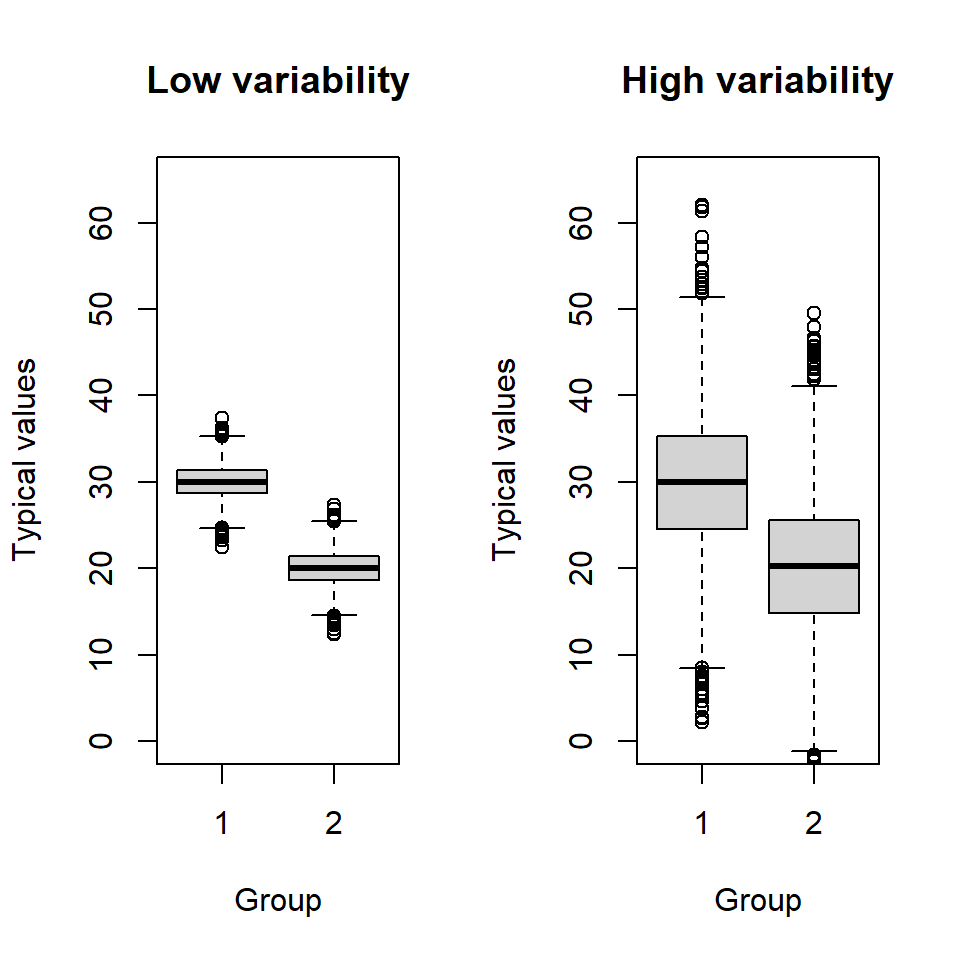
\includegraphics{IntroStats_files/figure-latex/groupbox-1} 

}

\caption{Box plots illustrating the distribution of data for two groups where the variability in the data is low (left) and high (right).}\label{fig:groupbox}
\end{figure}

We use the `test statistic' to quantify how much our data-estimate differs from the value in the null hypothesis taking into account the variability in the data. The formula for calculating the test statistic varies across data types and the nature of the test. In this chapter we consider one and two sample tests \(t\) to compare sample means; proportions are considered in a later chapter.

\hypertarget{one-sample-t-test}{%
\subsection{\texorpdfstring{One sample \(t\) test}{One sample t test}}\label{one-sample-t-test}}

In a one sample \(t\) test we compare the data-estimate to the hypothesised value; the \(t\) test statistic is given by:

\[t_{stat}=\frac{\hat \mu - \mu_0}{se(\hat \mu)}\]
where \(\hat \mu\) is the sample mean and \(se(\hat \mu)\) is the standard error of the sample mean.\\
Let's return to the example where we want to determine whether sample of baby weights could have been generated from a population with a mean of 120 ounces. As a reminder, the null hypothesis is:

\(H_0\): \({\mu} = 120\)

We will consider a two-tailed test and so the alternative hypothesis is:

\(H_1\): \({\mu} \neq 120\)

The sample statistics are: \(\hat\mu\)=119.5769, \(s\)=18.236 and \(n\)=1236. Substituting in these values we can calculate the standard error and test statistic.

The standard error is given by:

\[se(\hat\mu) = \frac{s}{\sqrt{n}} = \frac{18.24}{\sqrt{1236}} = 0.519\]
The test statistic is, therefore,

\[t_{stat}=\frac{\hat{\mu} - 120}{se(\hat{\mu})} = \frac{119.577 - 120}{0.519} = -0.815\]

If \(H_0\) is true, the test statistic (\(t_{stat}\)) should be close to zero because the difference between the test statistic and the hypothesised value is small.

If \(H_0\) is false, the test statistic should be large (positive or negative) because the difference between the test statistic and the hypothesised value is large.

To decide if a test statistic is `large' under the null hypothesis, we compare the test statistic to a reference distribution and, not surprisingly for a \(t\) test, we use the \(t\) distribution. The shape of the \(t\) distribution depends on the degrees of freedom and for a one sample \(t\) test the degrees of freedom (\(df\)) are given by \(df = n - 1\). Using this reference distribution we can determine what values might typically arise.

Having found the test statistic for the one sample test of baby weights, we obtain the associated reference \(t\) distribution. The sample size is 1236, and so \(df = 1236 - 1 = 1235\), hence, the reference distribution is a \(t_{df=1235}\) distribution (Figure \ref{fig:tdist1235}). This figure shows that values close to zero are likely to occur and values smaller than -2, or greater than 2, are unlikely. Where the test statistic lies on the reference distribution indicates how typical it is given the null hypothesis.

The reference distribution can be used in two ways to determine the strength of evidence for the null hypothesis: by obtaining an exact \(p\)-value for the test statistic or using a pre-determined significance level.

\hypertarget{determining-an-exact-p-value}{%
\subsubsection{\texorpdfstring{Determining an exact \(p\)-value}{Determining an exact p-value}}\label{determining-an-exact-p-value}}

A \textbf{\(p\)-value} is the \textbf{probability} of observing a test statistic at least as extreme as the one observed, given the null hypothesis is true. Thus,

\begin{itemize}
\item
  a test statistic close to zero would be likely to occur if was no difference between the data-estimate and the hypothesised value (other than sampling variability) and thus the probability of observing such a value would be high.
\item
  a large, absolute value of the test statistic would be likely if there was a real difference between the data-estimate and the hypothesised value (over and above sampling variability) and thus the probability of observing such a value would be small.
\end{itemize}

A mathematical representation of the \(p\)-value for a two-tailed test is:

\[Pr(T \le -|t_{stat}|) + Pr(T \ge |t_{stat}|) \]
where \(T\) is a random variable distributed as \(t_{df}\).

Using the \(t_{df=1235}\) distribution, the \(p\)-value associated with the test statistic of -0.815 can be obtained (Figure \ref{fig:tdist1235}). We want the probability of a value smaller than -0.815 and the probability of a value greater than 0.815 (i.e.~the areas in both tails of the distribution):

\[Pr(T \le -0.815) + Pr(T \ge 0.815) \]

The first part of this expression (i.e.~\(Pr(T \le -0.815)\)) is the cumulative distribution function and because the distribution is symmetric we can easily find the value \(Pr(T \ge 0.815)\).

\begin{figure}[!htb]

{\centering 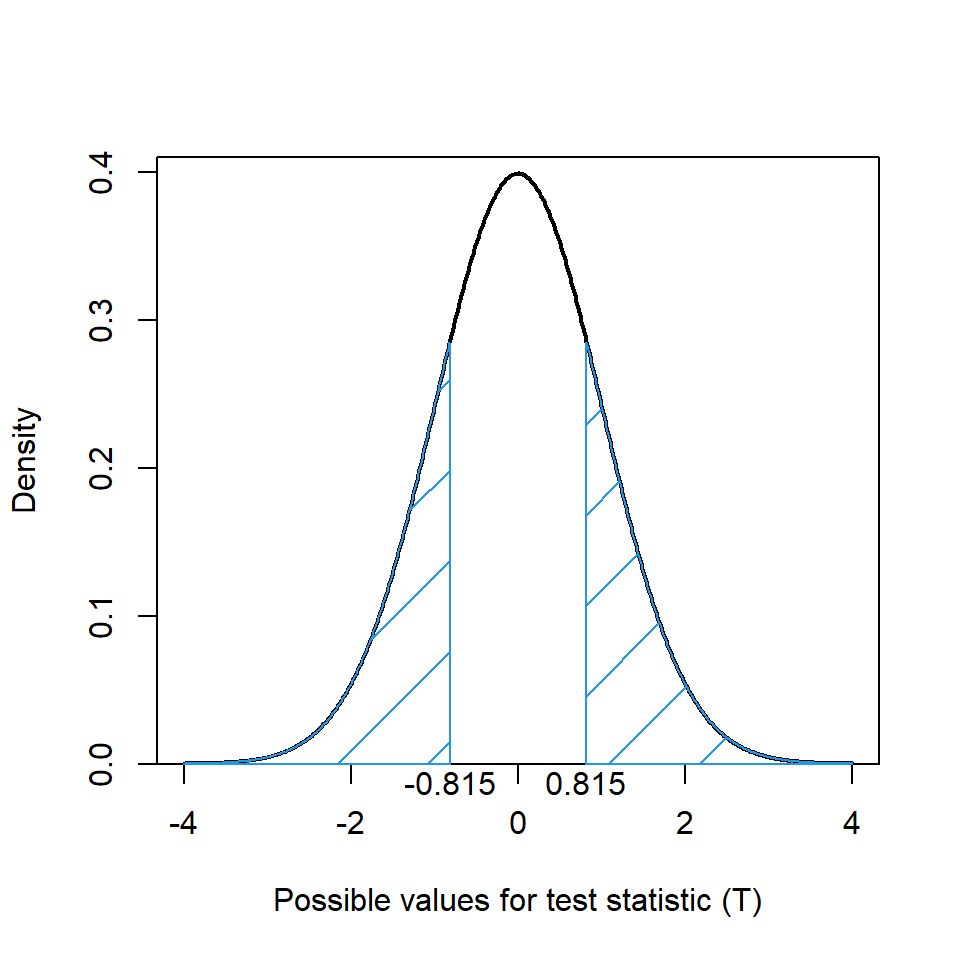
\includegraphics{IntroStats_files/figure-latex/tdist1235-1} 

}

\caption{Reference $t$ distribution for one sample example, $t_{df=1235}$. The blue shaded region indicates areas more extreme than the test statistic (for a two-tailed test).}\label{fig:tdist1235}
\end{figure}

The blue shaded area on Figure \ref{fig:tdist1235} is a substantial proportion of the total area and is, in fact, 0.415 (= 0.2076 + 0.2076) of the area, hence the \(p\)-value is 0.415. What does this \(p\)-value indicate about how likely a test statistic of -0.815 is?

The \(p\)-value measures the strength of evidence against the null hypothesis and, typically, \(H_0\) is only rejected when the \(p\)-value is really small. What is classed as small? Common threshold values are 0.1, 0.05 or 0.01 and they can be translated as follows \citep{wildgaf}:

\begin{longtable}[]{@{}ll@{}}
\toprule
Approximate \(p\)-value & Translation\tabularnewline
\midrule
\endhead
\textgreater0.10 & \textbf{No} evidence against \(H_0\)\tabularnewline
0.05 & \textbf{Weak} evidence against \(H_0\)\tabularnewline
0.01 & \textbf{Strong} evidence against \(H_0\)\tabularnewline
\(\le\) 0.001 & \textbf{Very strong} evidence against \(H_0\)\tabularnewline
\bottomrule
\end{longtable}

A \(p\)-value of 0.415 is pretty large, much larger than any of the values which provide evidence against \(H_0\) (shown in the table above). Hence, we conclude that the test statistic is consistent with \(H_0\); we are pretty likely to observe a test statistic of -0.815, or one more extreme. These data do not provide evidence to reject the null hypothesis and the sample of baby weights could come from an underlying population with a mean of 120 ounces.

\textbf{Example} The average age of the mothers in the sample (of size \(n=1236\)) from the US was 27.255 years with a standard deviation of 5.7814 years. The average age of first time mothers in the UK 2017 was 28.8 (The original data are \href{https://www.ons.gov.uk/peoplepopulationandcommunity/birthsdeathsandmarriages/livebirths/bulletins/birthcharacteristicsinenglandandwales/2017.html}{here}). Is there evidence to suggest that the age of mothers differ between the US and UK? We assume that the age of mothers in the UK was obtained from a census (and so there is no uncertainty).

The null hypothesis is:

\[H_0: \mu_{US} = 28.8\]

and since there is no reason to suspect that the average age in the US is either higher or lower than in the UK, we consider a two-tailed test and so the alternative hypothesis is:

\[H_1: \mu_{US} \ne 28.8\]

The standard error is given by:

\[se(\hat \mu_{US}) = \frac{s}{\sqrt{n}} = \frac{5.7814}{\sqrt{1236}} = 0.1644\]

and thus the test statistic is:

\[ t_{stat} = \frac{\hat \mu_{US} - 28.8}{se(\hat \mu_{US})} = \frac{27.255 - 28.8}{0.1664} = -9.285\]

We compare this to a reference distribution - since the sample size is 1236, the degrees of freedom for the reference distribution will be 1235. This is the distribution plotted in Figure \ref{fig:tdist1235} (since the sample size is the same as the sample of baby weights) and shows that a value of -9.285 will be out in the left hand tail (so much so that it is not even displayed on the \(x\)-axis scale.) In fact, the probability of obtaining a value as extreme, or more extreme, than -9.285 (i.e.~\(Pr(T \le -0.9285)\)) is pretty much zero and even when added to the probability in right hand tail (i.e.~\(Pr(T \ge 0.9285)\)) the \(p\)-value is approximately zero. Translating this value using the table above, there is strong evidence to reject \(H_0\) and conclude that the average age of the US mothers is not from a population with a mean of 28.8 years.

\hypertarget{using-a-fixed-significance-level}{%
\subsubsection{Using a fixed significance level}\label{using-a-fixed-significance-level}}

Some studies used a (pre-determined) fixed significance level; the evidence for the null hypothesis is determined with a 5\% significance level, for example. We find a `critical value' from the reference distribution based on the significance level and compare the test statistic to this critical value. Let's return to the reference distribution for the baby weights and assume a fixed significance level of 5\%; this is a two-tailed test (as specified in the alternative hypothesis) and so we want to find the quantile (the critical value, \(t_{crit}\)) such that:

\[Pr(T \le -|t_{crit}|) + Pr(T \ge |t_{crit}|) = 0.05\]

In Figure \ref{fig:tdist1235ex2}, the critical value, \(t_{crit}\) is 1.96 (i.e.~the red shaded area is 5\% of the total area) and we can see that the test statistic does not fall within the red shaded region. Hence, the conclusion is the same as before, there is no evidence to reject the null hypothesis, testing at a 5\% significance level.

A test statistic falling within the red shaded region would be sufficiently unlikely (based on the significance level) to have occurred if the null hypothesis was true, hence, providing evidence to reject the null hypothesis.

\begin{figure}[!htb]

{\centering 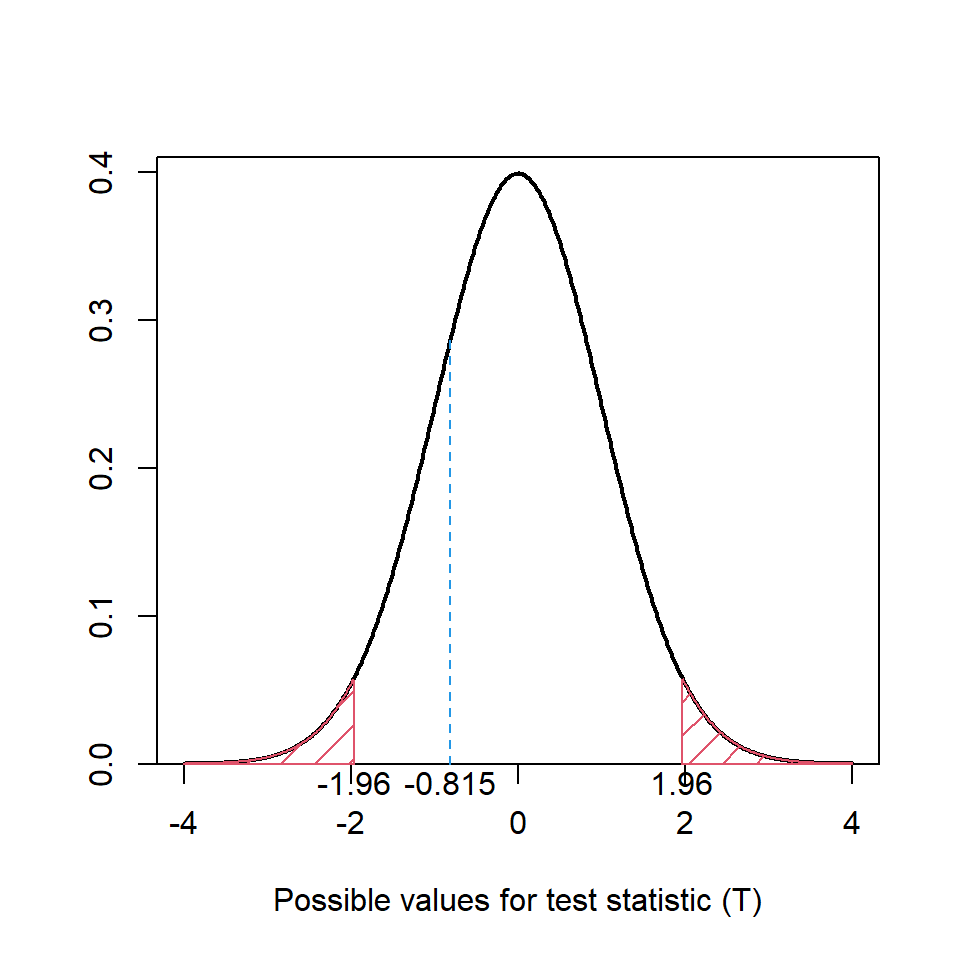
\includegraphics{IntroStats_files/figure-latex/tdist1235ex2-1} 

}

\caption{Reference t distribution for one sample example, $t_{df=1235}$. The red shaded region indicates areas more extreme than the critical value. The blue dashed line indicates the test statistic.}\label{fig:tdist1235ex2}
\end{figure}

This method of obtaining a critical value based on a fixed significance level and comparing it to the test statistic was used when making a decision regarding the null hypothesis was limited to looking up critical values in statistical tables. It is still frequently practised - it is commonplace to see the phrase `testing at a significance level of \ldots{}' in statistical reports. In more recent times, when access to computing power and statistical packages is commonplace, it is now easy to perform a test and obtain an exact \(p\)-value and indeed many computer packages routinely provide exact \(p\)-values in output.

\hypertarget{doing-this-in-r-12}{%
\subsubsection{Doing this in R}\label{doing-this-in-r-12}}

The function \texttt{t.test} was previously introduced to calculate a confidence interval; now we use it to perform a one sample \(t\) test on the baby weights. These data are stored in an object called \texttt{baby} and the weights are in a column called \texttt{bwt}. For a one sample test, the hypothesised value (\texttt{mu}) is specified and a two-tailed test (i.e.~\(H_1: \mu \ne 120\)) is performed by default.

\begin{Shaded}
\begin{Highlighting}[]
\CommentTok{\# One sample t test}
\FunctionTok{t.test}\NormalTok{(}\AttributeTok{x=}\NormalTok{baby}\SpecialCharTok{$}\NormalTok{bwt, }\AttributeTok{mu=}\DecValTok{120}\NormalTok{)}
\end{Highlighting}
\end{Shaded}

\begin{verbatim}
    One Sample t-test

data:  baby$bwt
t = -0.81574, df = 1235, p-value = 0.4148
alternative hypothesis: true mean is not equal to 120
95 percent confidence interval:
 118.5592 120.5945
sample estimates:
mean of x 
 119.5769 
\end{verbatim}

The output provides information about the test; the test statistic, degrees of freedom and exact \(p\)-value, what alternative hypothesis has been specified, and the sample mean and 95\% confidence interval for the sample mean.

The \texttt{t.test} function provides the \(p\)-value as part of the output, but we can also find this value from the \texttt{pt} function. In the command below, two alternative methods are used to find it.

\begin{Shaded}
\begin{Highlighting}[]
\CommentTok{\# Finding the exact p{-}value}
\CommentTok{\# 1. Calculate area in lower tail and multiply by 2}
\FunctionTok{pt}\NormalTok{(}\AttributeTok{q=}\SpecialCharTok{{-}}\FloatTok{0.815}\NormalTok{, }\AttributeTok{df=}\DecValTok{1235}\NormalTok{) }\SpecialCharTok{*} \DecValTok{2}
\end{Highlighting}
\end{Shaded}

\begin{verbatim}
[1] 0.4152294
\end{verbatim}

\begin{Shaded}
\begin{Highlighting}[]
\CommentTok{\# 2. Calculate area in both tails and add}
\FunctionTok{pt}\NormalTok{(}\AttributeTok{q=}\SpecialCharTok{{-}}\FloatTok{0.815}\NormalTok{, }\AttributeTok{df=}\DecValTok{1235}\NormalTok{) }\SpecialCharTok{+} \FunctionTok{pt}\NormalTok{(}\AttributeTok{q=}\FloatTok{0.815}\NormalTok{, }\AttributeTok{df=}\DecValTok{1235}\NormalTok{, }\AttributeTok{lower.tail=}\ConstantTok{FALSE}\NormalTok{)}
\end{Highlighting}
\end{Shaded}

\begin{verbatim}
[1] 0.4152294
\end{verbatim}

The \texttt{t.test} function does not provide the critical value but this can be obtained from the \texttt{qt} function: for a two-tailed test, the significance level is distributed equally between the two tails. For a significance level of 5\%, there will be 2.5\% in each tail; by default, the area in the lower tail is provided.

\begin{Shaded}
\begin{Highlighting}[]
\CommentTok{\# Left hand (lower) tail}
\FunctionTok{qt}\NormalTok{(}\AttributeTok{p=}\FloatTok{0.025}\NormalTok{, }\AttributeTok{df=}\DecValTok{1235}\NormalTok{)}
\end{Highlighting}
\end{Shaded}

\begin{verbatim}
[1] -1.961887
\end{verbatim}

\begin{Shaded}
\begin{Highlighting}[]
\CommentTok{\# Right hand (upper) tail}
\FunctionTok{qt}\NormalTok{(}\AttributeTok{p=}\FloatTok{0.025}\NormalTok{, }\AttributeTok{df=}\DecValTok{1235}\NormalTok{, }\AttributeTok{lower.tail=}\ConstantTok{FALSE}\NormalTok{)}
\end{Highlighting}
\end{Shaded}

\begin{verbatim}
[1] 1.961887
\end{verbatim}

\textbf{Q8.1} The weight of a chocolate bar was supposed to be 100 grams. To check the manufacturing process, a random sample of 100 bars were weighed; the sample mean was 99.06 grams and the standard deviation was 9.58.

\textbf{a.} State the null and alternative hypotheses to be tested with a two-tailed test.

\textbf{b.} Calculate a test statistic.

\textbf{c.} Based the following information, what do you conclude?

\begin{Shaded}
\begin{Highlighting}[]
\FunctionTok{qt}\NormalTok{(}\AttributeTok{p=}\FloatTok{0.025}\NormalTok{, }\AttributeTok{df=}\DecValTok{99}\NormalTok{)}
\end{Highlighting}
\end{Shaded}

\begin{verbatim}
[1] -1.984217
\end{verbatim}

\textbf{d.} What command would you use to calculate the exact \(p\)-value associated with the test statistic?

\hypertarget{two-sample-t-test}{%
\section{\texorpdfstring{Two sample \(t\) test}{Two sample t test}}\label{two-sample-t-test}}

In a two sample \(t\) test, we are interested in comparing means of continuous data from two groups (e.g.~groups \(A\) and \(B\)). The test statistic is used to quantify the discrepancy between the data-estimate and the null hypothesis (i.e.~no differences between the two means):
\[H_0 : \mu_A = \mu_B\]
or equivalently,

\[H_0 : \mu_A - \mu_B = 0\]
The alternative hypothesis for a two-tailed test will be:
\[H_1 : \mu_A - \mu_B \ne 0\]

The test statistic is given by:

\[t_{stat} = \frac{(\hat{\mu}_A - \hat{\mu}_B) - 0}{se(\hat{\mu}_A - \hat{\mu}_B)}\]

\textbf{Example} We continue to look at data collected from the observational study of birth weights introduced previously. We want to test whether babies born to mothers who did not smoke are heavier in weight compared to babies born to mothers who smoked. The summary data are provided in Table \ref{tab:babywgttab2}.

\begin{longtable}[]{@{}cccc@{}}
\caption{\label{tab:babywgttab2} Summary of birth weight data for the smoking and non-smoking groups (units are ounces).}\tabularnewline
\toprule
\begin{minipage}[b]{(\columnwidth - 3\tabcolsep) * \real{0.14}}\centering
Smoking\strut
\end{minipage} & \begin{minipage}[b]{(\columnwidth - 3\tabcolsep) * \real{0.08}}\centering
n\strut
\end{minipage} & \begin{minipage}[b]{(\columnwidth - 3\tabcolsep) * \real{0.12}}\centering
Mean\strut
\end{minipage} & \begin{minipage}[b]{(\columnwidth - 3\tabcolsep) * \real{0.12}}\centering
SD\strut
\end{minipage}\tabularnewline
\midrule
\endfirsthead
\toprule
\begin{minipage}[b]{(\columnwidth - 3\tabcolsep) * \real{0.14}}\centering
Smoking\strut
\end{minipage} & \begin{minipage}[b]{(\columnwidth - 3\tabcolsep) * \real{0.08}}\centering
n\strut
\end{minipage} & \begin{minipage}[b]{(\columnwidth - 3\tabcolsep) * \real{0.12}}\centering
Mean\strut
\end{minipage} & \begin{minipage}[b]{(\columnwidth - 3\tabcolsep) * \real{0.12}}\centering
SD\strut
\end{minipage}\tabularnewline
\midrule
\endhead
\begin{minipage}[t]{(\columnwidth - 3\tabcolsep) * \real{0.14}}\centering
No\strut
\end{minipage} & \begin{minipage}[t]{(\columnwidth - 3\tabcolsep) * \real{0.08}}\centering
742\strut
\end{minipage} & \begin{minipage}[t]{(\columnwidth - 3\tabcolsep) * \real{0.12}}\centering
123.05\strut
\end{minipage} & \begin{minipage}[t]{(\columnwidth - 3\tabcolsep) * \real{0.12}}\centering
17.4\strut
\end{minipage}\tabularnewline
\begin{minipage}[t]{(\columnwidth - 3\tabcolsep) * \real{0.14}}\centering
Yes\strut
\end{minipage} & \begin{minipage}[t]{(\columnwidth - 3\tabcolsep) * \real{0.08}}\centering
484\strut
\end{minipage} & \begin{minipage}[t]{(\columnwidth - 3\tabcolsep) * \real{0.12}}\centering
114.11\strut
\end{minipage} & \begin{minipage}[t]{(\columnwidth - 3\tabcolsep) * \real{0.12}}\centering
18.1\strut
\end{minipage}\tabularnewline
\bottomrule
\end{longtable}

We define the null hypothesis for the two groups, smokers (\(S\)) and non-smokers (\(N\)) as:

\[H_0: \mu_N - \mu_S = 0\]

The alternative hypothesis will be one-tailed because we want to see if babies in the non-smoking group are heavier than the smoking group babies.

\[H_1: \mu_N > \mu_S\]
or

\[H_1: \mu_N - \mu_S > 0\]

Since we do not want to make the assumption that the standard deviations of the two groups are equal, we will calculate the standard error of the difference from:

\[se(\hat{\mu_N} - \hat{\mu_S})= \sqrt{\frac{{s_N}^2}{{n_N}} + \frac{{s_S}^2}{{n_S}}} = \sqrt{\frac{17.4^2}{742} + \frac{18.1^2}{484}} = 1.042\]
Thus, the test statistic is:

\[t_{stat} = \frac{(123.05 - 114.11) - 0}{1.042} = 8.583\]

The degrees of freedom (for hand calculation) are given by finding the minimum value (\(Min\)) from the sample sizes for the two groups minus one:

\[df = Min(n_N-1, n_S-1) = Min(741, 483) = 483\]

Hence, the reference distribution is \(t_{df=483}\) and, because we are conducting a one-tail test, we are only interested in the probability associated with \(Pr(T \ge 8.583)\). Figure \ref{fig:tdist483} shows that this probability is going to be very small because the test statistic is in the extreme right hand tail, i.e.~the \(p\)-value is going to be close to zero. Hence, there is strong evidence to reject the null hypothesis and conclude that the babies from non-smoking mothers are heavier from smoking mothers.

\begin{figure}[!htb]

{\centering 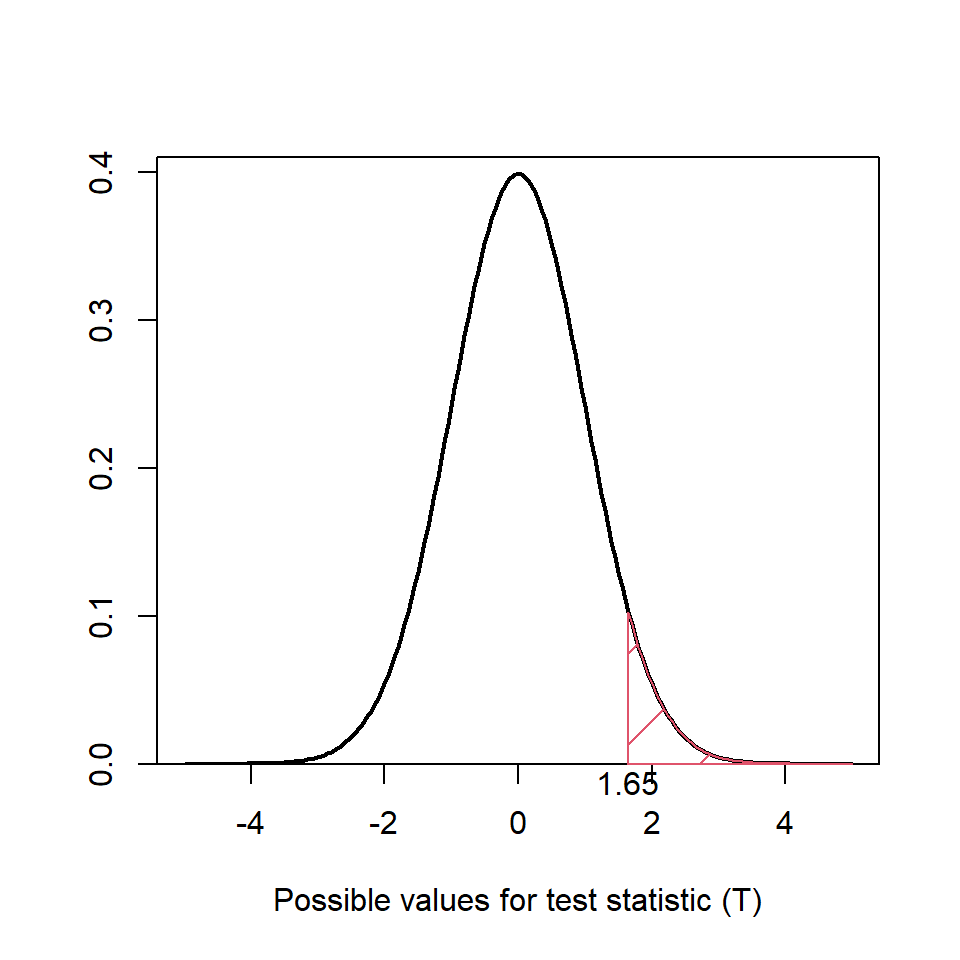
\includegraphics{IntroStats_files/figure-latex/tdist483-1} 

}

\caption{Reference $t$ distribution for two sample test example, $t_{df=483}$. The red shaded region indicates areas more extreme than the critical value.}\label{fig:tdist483}
\end{figure}

To obtain the critical value associated with a significance level of 5\%, we want the area in the right hand tail only - because this is a one-tailed test, i.e.~\(Pr(T > t_{crit}) = 0.05\); this is the red shaded area in Figure \ref{fig:tdist483}. The test statistic is much larger than the critical value (\(t_{crit}=1.65\)) and thus there is evidence to suggest that the babies born to non-smoking mothers are heavier than babies born to mothers who smoked, testing at a 5\% significance level.

\hypertarget{doing-this-in-r-13}{%
\subsection{Doing this in R}\label{doing-this-in-r-13}}

To make the code simple, separate objects are created for two groups. By default, a two-tailed test is performed but a one-tailed test can be specified using the \texttt{alternative} argument. Also by default, the standard deviations are assumed to be unequal and the degrees of freedom will be calculated using the Welch-Satterthwaite equation (Chapter \ref{CIformean}).

\begin{Shaded}
\begin{Highlighting}[]
\CommentTok{\# Save objects for two groups}
\NormalTok{grpN }\OtherTok{\textless{}{-}}\NormalTok{ baby}\SpecialCharTok{$}\NormalTok{bwt[baby}\SpecialCharTok{$}\NormalTok{smoke}\SpecialCharTok{==}\DecValTok{0}\NormalTok{]}
\NormalTok{grpS }\OtherTok{\textless{}{-}}\NormalTok{ baby}\SpecialCharTok{$}\NormalTok{bwt[baby}\SpecialCharTok{$}\NormalTok{smoke}\SpecialCharTok{==}\DecValTok{1}\NormalTok{]}

\CommentTok{\# Two sample, one{-}tailed t test}
\FunctionTok{t.test}\NormalTok{(}\AttributeTok{x=}\NormalTok{grpN, }\AttributeTok{y=}\NormalTok{grpS, }\AttributeTok{alternative=}\StringTok{"greater"}\NormalTok{)}
\end{Highlighting}
\end{Shaded}

\begin{verbatim}
    Welch Two Sample t-test

data:  grpN and grpS
t = 8.5813, df = 1003.2, p-value < 2.2e-16
alternative hypothesis: true difference in means is greater than 0
95 percent confidence interval:
 7.222928      Inf
sample estimates:
mean of x mean of y 
 123.0472  114.1095 
\end{verbatim}

Since a one-tailed test has been specified, only one limit of the confidence interval for the difference in means is provided; in this example it is a plausible value for a lower limit i.e.~that the weight of babies born to non-smoking mothers is likely to be at least 7.22 ounces.

The \(p\)-value in the output is found from:

\begin{Shaded}
\begin{Highlighting}[]
\CommentTok{\# p{-}value in upper tail (using the Welch{-}Satterthwaite df)}
\FunctionTok{pt}\NormalTok{(}\AttributeTok{q=}\FloatTok{8.5813}\NormalTok{, }\AttributeTok{df=}\FloatTok{1003.2}\NormalTok{, }\AttributeTok{lower.tail=}\ConstantTok{FALSE}\NormalTok{)}
\end{Highlighting}
\end{Shaded}

\begin{verbatim}
[1] 1.762554e-17
\end{verbatim}

The critical value, testing at a significance level of 5\% for a one-tailed test, would be found using the following command:

\begin{Shaded}
\begin{Highlighting}[]
\CommentTok{\# Critical value (using df for hand calculation)}
\CommentTok{\# Significance level is 5\% for a one{-}tailed test}
\FunctionTok{qt}\NormalTok{(}\AttributeTok{p=}\FloatTok{0.05}\NormalTok{, }\AttributeTok{df=}\DecValTok{482}\NormalTok{, }\AttributeTok{lower.tail=}\ConstantTok{FALSE}\NormalTok{)}
\end{Highlighting}
\end{Shaded}

\begin{verbatim}
[1] 1.648021
\end{verbatim}

\textbf{Q8.2} According to an advertising campaign, batteries from brand \(A\) last longer than
batteries from brand \(B\). State the null and alternative hypotheses required to test this claim and hence, conduct a hypothesis test using the following data using a fixed significance level of 5\%. Assume that the data are normally distributed. The following may be of use.

\begin{Shaded}
\begin{Highlighting}[]
\FunctionTok{qt}\NormalTok{(}\AttributeTok{p=}\FloatTok{0.05}\NormalTok{, }\AttributeTok{df=}\DecValTok{59}\NormalTok{, }\AttributeTok{lower.tail=}\ConstantTok{FALSE}\NormalTok{)}
\end{Highlighting}
\end{Shaded}

\begin{verbatim}
[1] 1.671093
\end{verbatim}

\begin{longtable}[]{@{}cccc@{}}
\toprule
\begin{minipage}[b]{(\columnwidth - 3\tabcolsep) * \real{0.11}}\centering
Brand\strut
\end{minipage} & \begin{minipage}[b]{(\columnwidth - 3\tabcolsep) * \real{0.07}}\centering
n\strut
\end{minipage} & \begin{minipage}[b]{(\columnwidth - 3\tabcolsep) * \real{0.10}}\centering
Mean\strut
\end{minipage} & \begin{minipage}[b]{(\columnwidth - 3\tabcolsep) * \real{0.10}}\centering
SD\strut
\end{minipage}\tabularnewline
\midrule
\endhead
\begin{minipage}[t]{(\columnwidth - 3\tabcolsep) * \real{0.11}}\centering
A\strut
\end{minipage} & \begin{minipage}[t]{(\columnwidth - 3\tabcolsep) * \real{0.07}}\centering
90\strut
\end{minipage} & \begin{minipage}[t]{(\columnwidth - 3\tabcolsep) * \real{0.10}}\centering
49.5\strut
\end{minipage} & \begin{minipage}[t]{(\columnwidth - 3\tabcolsep) * \real{0.10}}\centering
6.32\strut
\end{minipage}\tabularnewline
\begin{minipage}[t]{(\columnwidth - 3\tabcolsep) * \real{0.11}}\centering
B\strut
\end{minipage} & \begin{minipage}[t]{(\columnwidth - 3\tabcolsep) * \real{0.07}}\centering
60\strut
\end{minipage} & \begin{minipage}[t]{(\columnwidth - 3\tabcolsep) * \real{0.10}}\centering
46.1\strut
\end{minipage} & \begin{minipage}[t]{(\columnwidth - 3\tabcolsep) * \real{0.10}}\centering
3.31\strut
\end{minipage}\tabularnewline
\bottomrule
\end{longtable}

\textbf{Q8.3} An experiment looked at the effect of either a high or low protein diet on female rats. The gains in weight over a period of time were recorded and a two-sample \(t\) test was conducted; the R output is shown below.

\begin{verbatim}
    Welch Two Sample t-test

data:  hi.protein and lo.protein
t = 1.9107, df = 13.082, p-value = 0.07821
alternative hypothesis: true difference in means is not equal to 0
95 percent confidence interval:
 -2.469073 40.469073
sample estimates:
mean of x mean of y 
      120       101 
\end{verbatim}

\textbf{a.} State the null and alternative hypotheses that have been tested.

\textbf{b.} Given that the standard error for the difference in means used in this test was 9.944, explain how the test statistic was calculated.

\textbf{c.} Interpret the test results.

\hypertarget{paired-t-test}{%
\section{\texorpdfstring{Paired \(t\) test}{Paired t test}}\label{paired-t-test}}

A paired \(t\) test is used to compare the population means of two groups where the observations in one sample can be paired with an observation in the other sample. An example would be a study where participants are measured before and after a treatment and so the two measurments are not independent since the measurements were taken from the same participants. These types of study can be very useful because using the same participants can eliminate any variation other than the treatment between the two groups.

Let \(x\) be a measurement before treatment, or some intervention, and \(y\) be a measurement after treatment. The difference between the two measurements on each participant \(i\) is given by:

\[d_i = x_i - y_i\]

The mean of the difference is calculated, here denoted by \(\bar d\), this essentially reduces the data to one sample; a paired \(t\) test is the same as a one sample \(t\) test on the differences. The null hypothesis is that the true mean of the differences is equal to zero:

\[H_0: \mu_d = 0\]
The alternative hypothesis can be specified in several ways depending on whether a one or two-tailed test is required, for example:

\[H_1: \mu_d \ne 0\]
\[H_1: \mu_d > 0\]
\[H_1: \mu_d < 0\]

The test statistic is given by:

\[t_{stat} = \frac{\bar d - 0}{se(\bar d)} \]

The standard error of the differences is:

\[se(\bar d) = \frac{s_d}{\sqrt{n}}\]
where \(s_d\) is the sample standard deviation of the differences.

Under the null hypothesis, the test statistic follows a \(t_{df=n-1}\) distribution and this can be used to obtain a \(p\)-value.

\textbf{Example} A study tested whether cholesterol level was reduced after using a certain brand of margarine as part of a low cholesterol diet. Eighteen participants incorporated the margarine into their daily diet and their cholesterol levels were measured at the start and after 4 and 8 weeks. Here we compare the cholesterol levels after 4 and 8 weeks (data can be found \href{https://www.sheffield.ac.uk/mash/statistics/datasets}{here}). We do not make an assumption about whether cholesterol levels should be higher or lower after 8 weeks and hence use a two-tailed test.

The mean and standard deviation of the differences are \(\bar d = 0.0628\) and \(s_d = 0.0704\). The test statistic is then:

\[t_{stat} = \frac{0.0628}{\frac{0.0704}{\sqrt{18}}} = 3.78\]
This is compared to a \(t_{df=17}\) distribution; Figure \ref{fig:tdist17} shows that the test statistic lies in the right hand tail and so the probability of obtaining a value as extreme as this is going to be very small. The critical value is 2.11 and Figure \ref{fig:tdist17} shows that the test statistic is much greater than the critical value. Therefore, there is some evidence to reject the null hypothesis and conclude that there is a difference in cholesterol levels between weeks 4 and 8.

\begin{figure}[!htb]

{\centering 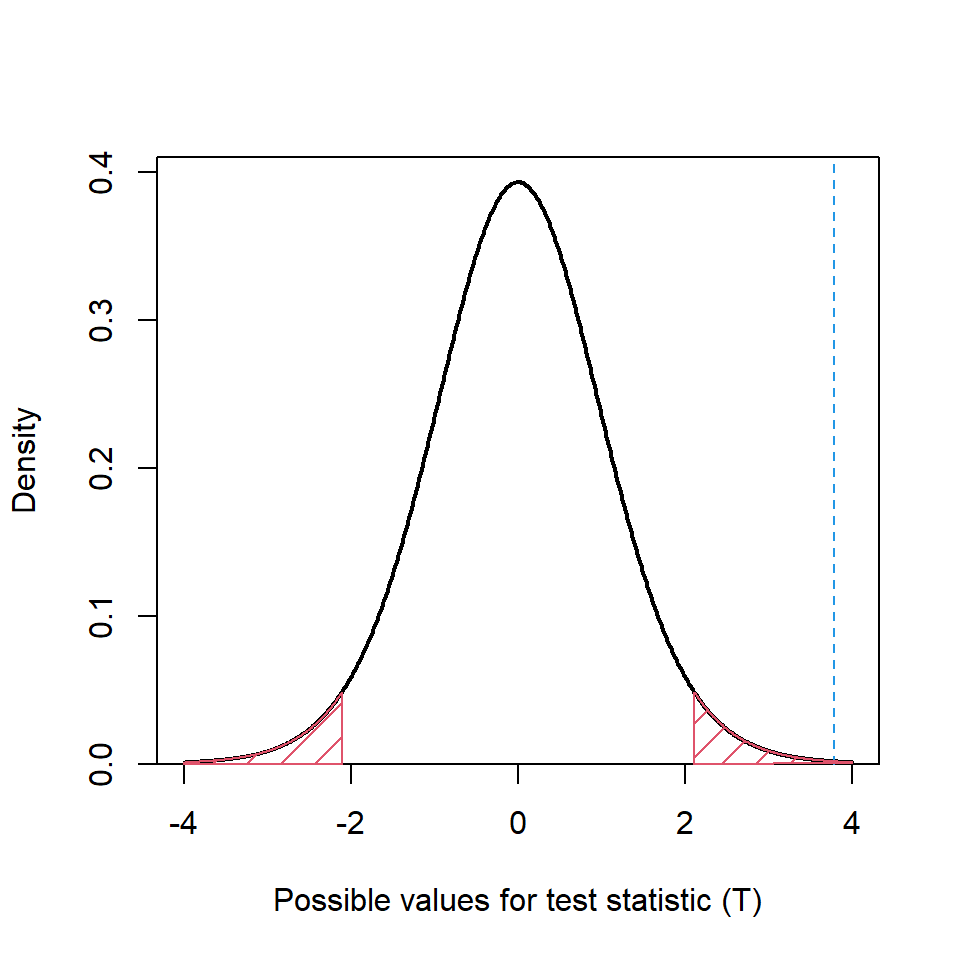
\includegraphics{IntroStats_files/figure-latex/tdist17-1} 

}

\caption{Reference $t_{df}=17$ distribution for paired sample example. The blue dashed line indicates the test statistic and the red shaded region indicates areas more extreme than the critical value (testing at a significance level of 5\%.}\label{fig:tdist17}
\end{figure}

\hypertarget{doing-this-in-r-14}{%
\subsection{Doing this in R}\label{doing-this-in-r-14}}

The \texttt{t.test} function is used to perform a paired \(t\) test with an additional argument to indicate that the data are paired observations. In the example below, the cholesterol data have been stored in an object called \texttt{chol}.

\begin{Shaded}
\begin{Highlighting}[]
\CommentTok{\# Paired t test}
\FunctionTok{t.test}\NormalTok{(chol}\SpecialCharTok{$}\NormalTok{After8weeks, chol}\SpecialCharTok{$}\NormalTok{After4weeks, }\AttributeTok{paired=}\ConstantTok{TRUE}\NormalTok{)}
\end{Highlighting}
\end{Shaded}

\begin{verbatim}
    Paired t-test

data:  chol$After8weeks and chol$After4weeks
t = -3.7809, df = 17, p-value = 0.001491
alternative hypothesis: true difference in means is not equal to 0
95 percent confidence interval:
 -0.09780897 -0.02774658
sample estimates:
mean of the differences 
            -0.06277778 
\end{verbatim}

The similarity between this approach and using a one sample test of the differences is easily shown:

\begin{Shaded}
\begin{Highlighting}[]
\CommentTok{\# Calculate the difference}
\NormalTok{diff }\OtherTok{\textless{}{-}}\NormalTok{ chol}\SpecialCharTok{$}\NormalTok{After8weeks }\SpecialCharTok{{-}}\NormalTok{ chol}\SpecialCharTok{$}\NormalTok{After4weeks }

\CommentTok{\# One sample t test of differences}
\FunctionTok{t.test}\NormalTok{(}\AttributeTok{x=}\NormalTok{diff, }\AttributeTok{mu=}\DecValTok{0}\NormalTok{)}
\end{Highlighting}
\end{Shaded}

\begin{verbatim}
    One Sample t-test

data:  diff
t = -3.7809, df = 17, p-value = 0.001491
alternative hypothesis: true mean is not equal to 0
95 percent confidence interval:
 -0.09780897 -0.02774658
sample estimates:
  mean of x 
-0.06277778 
\end{verbatim}

\hypertarget{t-test-assumptions}{%
\section{\texorpdfstring{\(t\) test assumptions}{t test assumptions}}\label{t-test-assumptions}}

Both one and two sample \(t\) tests are based on assumptions that need to be fulfilled for the results to be reliable. These assumptions are that the data are

\begin{enumerate}
\def\labelenumi{\arabic{enumi}.}
\item
  independent (both within and between groups), and
\item
  normally distributed.
\end{enumerate}

The first assumption can be determined by having knowledge of the data collection procedures and what the data represent. If the sampling units in the groups are paired, then a paired \(t\) test can be undertaken.

The second assumption can be checked by plotting the data, for example using histograms and boxplots. This will be explored further in the chapter \ref{anova}.

If the data are not normally distributed, then a non-parametric test can be used and so we look at this next.

\textbf{Q8.4} For the test described in Q8.3, as well as an assumption regarding standard deviations of the two groups, state two other assumptions on which this test was based.

\hypertarget{non-parametric-alternative-to-t-tests}{%
\section{\texorpdfstring{Non-parametric alternative to \(t\) tests}{Non-parametric alternative to t tests}}\label{non-parametric-alternative-to-t-tests}}

The \(t\) test assumes that the data are normally distributed and, although the test is quite robust if data are not exactly normally distributed (i.e.~the test result is still valid), in some situations the data will be skewed or the sample size will be small. In these circumstances, non-parametric, or distribution-free, methods are available. However, these methods still assume that the data are independent within and between groups.

To determine if two data samples have the same population mean, the Mann-Whitney-Wilcoxon test is used.

\hypertarget{mann-whitney-wilcoxon-test}{%
\subsection{Mann-Whitney-Wilcoxon test}\label{mann-whitney-wilcoxon-test}}

This test is known by various names (e.g.~Mann-Whitney, two-sample Wilcoxon). The null hypothesis is that the two groups (say \(A\) and \(B\)) have the same distributions - represented as \(H_0: A = B\). The alternative hypothesis is that there is a shift in the distribution; if there is no reason to suggest a shift to the left or right, the alternative hypothesis will \(H_1: A \ne B\). One-tailed variants (i.e.~\(H_1: A < B\) or \(H_1: A > B\)) can also be tested.

\textbf{Example} To illustrate the test procedure, six baby weights from the smoking group and six from the non-smoking group are used. The data in the two groups are

Non-smoking (N): 120, 113, 123, 136, 138, 132

Smoking (S): 128, 108, 143, 144, 141, 110

The test statistic is based on sorting the data into order and assigning ranks - the ranks in each group are then added together. The procedure is:

\begin{enumerate}
\def\labelenumi{\arabic{enumi}.}
\tightlist
\item
  Combine the values (weights) from both groups and rank them in order of increasing value.
\end{enumerate}

\begin{longtable}[]{@{}ccc@{}}
\toprule
\begin{minipage}[b]{(\columnwidth - 2\tabcolsep) * \real{0.12}}\centering
Weight\strut
\end{minipage} & \begin{minipage}[b]{(\columnwidth - 2\tabcolsep) * \real{0.11}}\centering
Group\strut
\end{minipage} & \begin{minipage}[b]{(\columnwidth - 2\tabcolsep) * \real{0.11}}\centering
Rank\strut
\end{minipage}\tabularnewline
\midrule
\endhead
\begin{minipage}[t]{(\columnwidth - 2\tabcolsep) * \real{0.12}}\centering
108\strut
\end{minipage} & \begin{minipage}[t]{(\columnwidth - 2\tabcolsep) * \real{0.11}}\centering
S\strut
\end{minipage} & \begin{minipage}[t]{(\columnwidth - 2\tabcolsep) * \real{0.11}}\centering
1\strut
\end{minipage}\tabularnewline
\begin{minipage}[t]{(\columnwidth - 2\tabcolsep) * \real{0.12}}\centering
110\strut
\end{minipage} & \begin{minipage}[t]{(\columnwidth - 2\tabcolsep) * \real{0.11}}\centering
S\strut
\end{minipage} & \begin{minipage}[t]{(\columnwidth - 2\tabcolsep) * \real{0.11}}\centering
2\strut
\end{minipage}\tabularnewline
\begin{minipage}[t]{(\columnwidth - 2\tabcolsep) * \real{0.12}}\centering
113\strut
\end{minipage} & \begin{minipage}[t]{(\columnwidth - 2\tabcolsep) * \real{0.11}}\centering
N\strut
\end{minipage} & \begin{minipage}[t]{(\columnwidth - 2\tabcolsep) * \real{0.11}}\centering
3\strut
\end{minipage}\tabularnewline
\begin{minipage}[t]{(\columnwidth - 2\tabcolsep) * \real{0.12}}\centering
120\strut
\end{minipage} & \begin{minipage}[t]{(\columnwidth - 2\tabcolsep) * \real{0.11}}\centering
N\strut
\end{minipage} & \begin{minipage}[t]{(\columnwidth - 2\tabcolsep) * \real{0.11}}\centering
4\strut
\end{minipage}\tabularnewline
\begin{minipage}[t]{(\columnwidth - 2\tabcolsep) * \real{0.12}}\centering
123\strut
\end{minipage} & \begin{minipage}[t]{(\columnwidth - 2\tabcolsep) * \real{0.11}}\centering
N\strut
\end{minipage} & \begin{minipage}[t]{(\columnwidth - 2\tabcolsep) * \real{0.11}}\centering
5\strut
\end{minipage}\tabularnewline
\begin{minipage}[t]{(\columnwidth - 2\tabcolsep) * \real{0.12}}\centering
128\strut
\end{minipage} & \begin{minipage}[t]{(\columnwidth - 2\tabcolsep) * \real{0.11}}\centering
S\strut
\end{minipage} & \begin{minipage}[t]{(\columnwidth - 2\tabcolsep) * \real{0.11}}\centering
6\strut
\end{minipage}\tabularnewline
\begin{minipage}[t]{(\columnwidth - 2\tabcolsep) * \real{0.12}}\centering
132\strut
\end{minipage} & \begin{minipage}[t]{(\columnwidth - 2\tabcolsep) * \real{0.11}}\centering
N\strut
\end{minipage} & \begin{minipage}[t]{(\columnwidth - 2\tabcolsep) * \real{0.11}}\centering
7\strut
\end{minipage}\tabularnewline
\begin{minipage}[t]{(\columnwidth - 2\tabcolsep) * \real{0.12}}\centering
136\strut
\end{minipage} & \begin{minipage}[t]{(\columnwidth - 2\tabcolsep) * \real{0.11}}\centering
N\strut
\end{minipage} & \begin{minipage}[t]{(\columnwidth - 2\tabcolsep) * \real{0.11}}\centering
8\strut
\end{minipage}\tabularnewline
\begin{minipage}[t]{(\columnwidth - 2\tabcolsep) * \real{0.12}}\centering
138\strut
\end{minipage} & \begin{minipage}[t]{(\columnwidth - 2\tabcolsep) * \real{0.11}}\centering
N\strut
\end{minipage} & \begin{minipage}[t]{(\columnwidth - 2\tabcolsep) * \real{0.11}}\centering
9\strut
\end{minipage}\tabularnewline
\begin{minipage}[t]{(\columnwidth - 2\tabcolsep) * \real{0.12}}\centering
141\strut
\end{minipage} & \begin{minipage}[t]{(\columnwidth - 2\tabcolsep) * \real{0.11}}\centering
S\strut
\end{minipage} & \begin{minipage}[t]{(\columnwidth - 2\tabcolsep) * \real{0.11}}\centering
10\strut
\end{minipage}\tabularnewline
\begin{minipage}[t]{(\columnwidth - 2\tabcolsep) * \real{0.12}}\centering
143\strut
\end{minipage} & \begin{minipage}[t]{(\columnwidth - 2\tabcolsep) * \real{0.11}}\centering
S\strut
\end{minipage} & \begin{minipage}[t]{(\columnwidth - 2\tabcolsep) * \real{0.11}}\centering
11\strut
\end{minipage}\tabularnewline
\begin{minipage}[t]{(\columnwidth - 2\tabcolsep) * \real{0.12}}\centering
144\strut
\end{minipage} & \begin{minipage}[t]{(\columnwidth - 2\tabcolsep) * \real{0.11}}\centering
S\strut
\end{minipage} & \begin{minipage}[t]{(\columnwidth - 2\tabcolsep) * \real{0.11}}\centering
12\strut
\end{minipage}\tabularnewline
\bottomrule
\end{longtable}

\begin{enumerate}
\def\labelenumi{\arabic{enumi}.}
\setcounter{enumi}{1}
\tightlist
\item
  Calculate the sum of ranks for each group:
\end{enumerate}

\[R_N = 3 + 4 + 5 + 7 + 8 + 9 = 36\]
\[R_S = 1 + 2 + 6 + 10 + 11 + 12 = 42\]

\begin{enumerate}
\def\labelenumi{\arabic{enumi}.}
\setcounter{enumi}{2}
\tightlist
\item
  Calculate a test statistic for both groups:
\end{enumerate}

\[W_N = R_N - \frac{n_N(n_N + 1)}{2} = 36 - \frac{6 \times 7}{2} = 15\]

\[W_S = R_S - \frac{n_S(n_S + 1)}{2} = 42 - \frac{6 \times 7}{2} = 21\]

\begin{enumerate}
\def\labelenumi{\arabic{enumi}.}
\setcounter{enumi}{3}
\tightlist
\item
  Either of these values are used as the test statistic - the smaller value is generally used when consulting statistical tables to determine a critical value (There are some statistical tables \href{https://onlinepubs.trb.org/onlinepubs/nchrp/cd-22/manual/v2appendixc.pdf}{here}) and then the test statistic would be compared to the critical value as described previously. Here, we use R and R uses the test statistic for the first group specified in the command (see below).
\end{enumerate}

There are also one sample and paired sample variants of the Mann-Whitney-Wilcoxon test and these are illustrated below.

\hypertarget{doing-this-in-r-15}{%
\subsubsection{Doing this in R}\label{doing-this-in-r-15}}

The function is called \texttt{wilcox.test} and, as in the example above, only the first six weights in each group are used.

\begin{Shaded}
\begin{Highlighting}[]
\FunctionTok{wilcox.test}\NormalTok{(}\AttributeTok{x=}\NormalTok{grpN[}\DecValTok{1}\SpecialCharTok{:}\DecValTok{6}\NormalTok{], }\AttributeTok{y=}\NormalTok{grpS[}\DecValTok{1}\SpecialCharTok{:}\DecValTok{6}\NormalTok{])}
\end{Highlighting}
\end{Shaded}

\begin{verbatim}
    Wilcoxon rank sum exact test

data:  grpN[1:6] and grpS[1:6]
W = 15, p-value = 0.6991
alternative hypothesis: true location shift is not equal to 0
\end{verbatim}

The \(p\)-value is interpreted as before; here it is large and thus provides no evidence to reject the null hypothesis.

For large samples, the test statistic \(W\) is approximately normally distributed and so the \(p\)-value is obtained from the normal distribution and a correction is applied to account for this approximation: we can see this using all the data for the baby weights.

\begin{Shaded}
\begin{Highlighting}[]
\FunctionTok{wilcox.test}\NormalTok{(}\AttributeTok{x=}\NormalTok{grpN, }\AttributeTok{y=}\NormalTok{grpS)}
\end{Highlighting}
\end{Shaded}

\begin{verbatim}
    Wilcoxon rank sum test with continuity correction

data:  grpN and grpS
W = 231918, p-value < 2.2e-16
alternative hypothesis: true location shift is not equal to 0
\end{verbatim}

A one sample version is available; here the null hypothesis can be interpreted as the median is equal to some hypothesised value:

\[H_0: \textrm{median} = \textrm{median}_0\]

To illustrate the command for the baby weights:

\begin{Shaded}
\begin{Highlighting}[]
\FunctionTok{wilcox.test}\NormalTok{(}\AttributeTok{x=}\NormalTok{baby}\SpecialCharTok{$}\NormalTok{bwt, }\AttributeTok{mu=}\DecValTok{120}\NormalTok{)}
\end{Highlighting}
\end{Shaded}

\begin{verbatim}
    Wilcoxon signed rank test with continuity correction

data:  baby$bwt
V = 358753, p-value = 0.7062
alternative hypothesis: true location is not equal to 120
\end{verbatim}

To illustrate a paired sample variant of the Mann-Whitney-Wilcoxon test, we return to the cholesterol data.

\begin{Shaded}
\begin{Highlighting}[]
\CommentTok{\# Paired sample}
\FunctionTok{wilcox.test}\NormalTok{(}\AttributeTok{x=}\NormalTok{chol}\SpecialCharTok{$}\NormalTok{After4weeks, }\AttributeTok{y=}\NormalTok{chol}\SpecialCharTok{$}\NormalTok{After8weeks, }\AttributeTok{paired=}\ConstantTok{TRUE}\NormalTok{)}
\end{Highlighting}
\end{Shaded}

\begin{verbatim}
    Wilcoxon signed rank test with continuity correction

data:  chol$After4weeks and chol$After8weeks
V = 152.5, p-value = 0.003725
alternative hypothesis: true location shift is not equal to 0
\end{verbatim}

\hypertarget{practical-significance-versus-statistical-significance}{%
\section{Practical significance versus statistical significance}\label{practical-significance-versus-statistical-significance}}

The word `significant' can often cause confusion - in hypothesis tests a significant result frequently means the \(p\)-value is less than 0.05. It does not necessarily imply that the result (for example, a difference between means) is substantial and has practical significance. Indeed we sometimes define the significance as part of our test e.g.~0.05, and another analysis might use a different value to determine significance. To illustrate the practical significance, confidence intervals should be reported along with the test results.

Statistical significance:

\begin{itemize}
\item
  relates to the existence of an effect,
\item
  it can be found with small differences if the sample size is large enough (because the standard error will be small).
\end{itemize}

Practical (or clinical) significance:

\begin{itemize}
\tightlist
\item
  relates to the size of an effect and should be reported to provide context to the hypothesis test results.
\end{itemize}

For an interesting (and short) read about practical and statistical significance have a look at this \href{https://www.statslife.org.uk/the-statistics-dictionary/1000-the-statistics-dictionary-significantly-misleading}{Significance Magazine article}.

\hypertarget{SUMhyp}{%
\section{Summary}\label{SUMhyp}}

This chapter has covered the underlying concepts of hypothesis testing; a test statistic is obtained and compared to a reference distribution. Where the test statistic lies on this reference distribution provides evidence to either reject, or not reject, the null hypothesis. In terms of the \(p\)-value:

\begin{itemize}
\item
  a small \(p\)-value indicates that the test statistic is very unlikely to be obtained when the null hypothesis is true - \(H_0\) is rejected in favour of \(H_1\).
\item
  a large \(p\)-value indicates the test statistic is likely to be obtained when the null hypothesis is true - \(H_0\) cannot be rejected.
\end{itemize}

The \(t\) tests rely on data being normally distributed; if this is not a valid assumption, non-parametric tests can be used.

In chapter 11, we consider hypothesis tests for when there are more than two groups. For more information about hypothesis testing in general \href{https://www.khanacademy.org/math/probability/statistics-inferential/hypothesis-testing/v/hypothesis-testing-and-p-values}{see}.

\hypertarget{learning-outcomes-4}{%
\subsection{Learning outcomes}\label{learning-outcomes-4}}

In this chapter you have seen how to

\begin{enumerate}
\def\labelenumi{\arabic{enumi}.}
\item
  define test hypotheses and determine whether one-tailed or two-tailed tests should be used,
\item
  calculate a test statistic for a one, two and paired sample \(t\) tests,
\item
  decide whether to reject, or otherwise, the null hypothesis based on the \(p\)-value and testing at a fixed significance level,
\item
  use a non-parametric alternative to \(t\)-tests, and
\item
  consider the practical and statistical significance of a test.
\end{enumerate}

\hypertarget{ANShyp}{%
\section{Answers}\label{ANShyp}}

\textbf{Q8.1} The sample statistics were \(n\)=100, \(\hat \mu = 99.06\) and \(s=9.58\).

\textbf{Q8.1} \textbf{a.} We want to determine if the population mean could be 100 grams. The null and alternative hypotheses to be tested with a two-tailed test are:

\[H_0: \mu = 100\]

\[H_1: \mu \ne 100\]

\textbf{Q8.1} \textbf{b.} The test statistic is

\[t_{stat} = \frac{\hat \mu - m_0}{\frac{s}{\sqrt{n}}} = \frac{99.06 - 100}{\frac{9.58}{\sqrt{100}}} = -0.9812\]

\textbf{Q8.1} \textbf{c.} The value provided in the output (i.e.~-1.984) was the critical value (\(t{crit}\)) in the lower tail, testing at a fixed significance level of 5\%. In this case \(t_{crit} < t_{stat}\) and so there is no evidence to reject the null hypothesis; the sample could have been generated from a population with mean 100 grams.

\textbf{d.} The exact \(p\)-value associated with the test statistic for a two-tailed test will be provided by the command:

\begin{Shaded}
\begin{Highlighting}[]
\FunctionTok{pt}\NormalTok{(}\AttributeTok{q=}\SpecialCharTok{{-}}\FloatTok{0.9812}\NormalTok{, }\AttributeTok{df=}\DecValTok{99}\NormalTok{) }\SpecialCharTok{*} \DecValTok{2}
\end{Highlighting}
\end{Shaded}

\begin{verbatim}
[1] 0.3288859
\end{verbatim}

\textbf{Q8.2} The claim is that Brand A batteries last longer than Brand B. Therefore, the hypotheses will be:

\[H_0: \mu_A - \mu_B = 0\]

\[H_1: \mu_A - \mu_B > 0\]

The test statistic is given by

\[t_{stat} = \frac{(\hat \mu_A - \hat \mu_B) - 0}{se(\mu_A - \hat \mu_B)}\]

First calculate the standard error of the difference:

\[se(\hat{\mu_A} - \hat{\mu_B})= \sqrt{\frac{{s_A}^2}{{n_A}} + \frac{{s_B}^2}{{n_B}}} = \sqrt{\frac{6.32^2}{90} + \frac{3.31^2}{60}} = 0.7915\]
Thus, the test statistic is:

\[t_{stat} = \frac{(49.5 - 46.1) - 0}{0.7915} = 4.2956\]

For ease of calculation, the degrees of freedom for the relevant \(t\) distribution are given by:

\[df = Min(n_A - 1, n_B - 1) = Min(89, 59) = 59\]

The critical value will be found from R and since this is a one-tailed test, we only want the area in the upper tail.

\begin{Shaded}
\begin{Highlighting}[]
\FunctionTok{qt}\NormalTok{(}\AttributeTok{p=}\FloatTok{0.05}\NormalTok{, }\AttributeTok{df=}\DecValTok{59}\NormalTok{, }\AttributeTok{lower.tail=}\ConstantTok{FALSE}\NormalTok{)}
\end{Highlighting}
\end{Shaded}

\begin{verbatim}
[1] 1.671093
\end{verbatim}

This value is less than the test statistic and so there is evidence to reject the null hypothesis, testing at a 5\% significance level, and conclude that brand A lasts longer than brand B.

The \(p\)-value is found using the \texttt{pt} function:

\begin{Shaded}
\begin{Highlighting}[]
\FunctionTok{pt}\NormalTok{(}\AttributeTok{q=}\FloatTok{4.2956}\NormalTok{, }\AttributeTok{df=}\DecValTok{59}\NormalTok{, }\AttributeTok{lower.tail=}\ConstantTok{FALSE}\NormalTok{)}
\end{Highlighting}
\end{Shaded}

\begin{verbatim}
[1] 3.298826e-05
\end{verbatim}

In confirmation, the \(p\)-value is small (i.e.~\textless0.001).

\textbf{Q8.3} Let the two groups, high protein and low protein diets, be defined by \(H\) and \(L\), respectively.

\textbf{Q8.3} \textbf{a.} The null and alternative hypotheses are

\[H_0: \mu_H - \mu_L = 0\]
\[H_1: \mu_H - \mu_L \ne 0\]

\textbf{Q8.3} \textbf{b.} The test statistic was calculated from the data estimate (difference in means) minus the hypothesised value divided by the standard error of the difference.

\[\textrm{test statistic} = \frac{(\hat \mu_H - \hat \mu_L) - 0}{se(\hat \mu_H - \hat \mu_L)}\]

\[ 1.9107 =\frac{120 - 101}{9.944} \]
\textbf{Q8.3} \textbf{c.} The \(p\)-value is 0.07821 which provides weak evidence to reject the null hypothesis.

\textbf{Q8.4} The two remaining assumptions are:

\begin{enumerate}
\def\labelenumi{\arabic{enumi}.}
\item
  Independence of the data within and between groups.
\item
  Data are normally distributed.
\end{enumerate}

\hypertarget{anova}{%
\chapter{Analysis of Variance}\label{anova}}

{ \emph{The analysis of variance is not a mathematical theorem, but rather a convenient method of arranging the arithmetic.} R. A. Fisher. }

\hypertarget{INTanova}{%
\section{Introduction}\label{INTanova}}

Previously we have considered the comparison of two groups. In this chapter, we consider the comparison of more than two group means using a procedure called analysis of variance (generally called ANOVA). ANOVA indicates whether at least one group is different from at least one other group mean. To identify where those differences lie, we need to then consider each of the pairwise comparisons but taking into account that we are making several comparisons.

In this chapter we will consider

\begin{itemize}
\tightlist
\item
  the number of comparisons when there are more than two groups,
\item
  determining if there is a difference in the group means and where any differences might lie,
\item
  checking test assumptions and
\item
  alternative methods if the assumptions are not valid.
\end{itemize}

\hypertarget{multiple-comparisons}{%
\section{Multiple comparisons}\label{multiple-comparisons}}

We start with a motivating example; a sample of plants have been grown in three different growing mediums and the amounts of various chemical elements in a leaf from each plant have been obtained. It was felt that the chemical composition of the plants was specific to growing medium and, if so, this may help identify where plants were grown. The growing mediums, or groups, were classified as B, N and P and here, we are interested in whether the mean titanium levels differ between the three groups (Figure \ref{fig:plantbox}).

\begin{figure}

{\centering 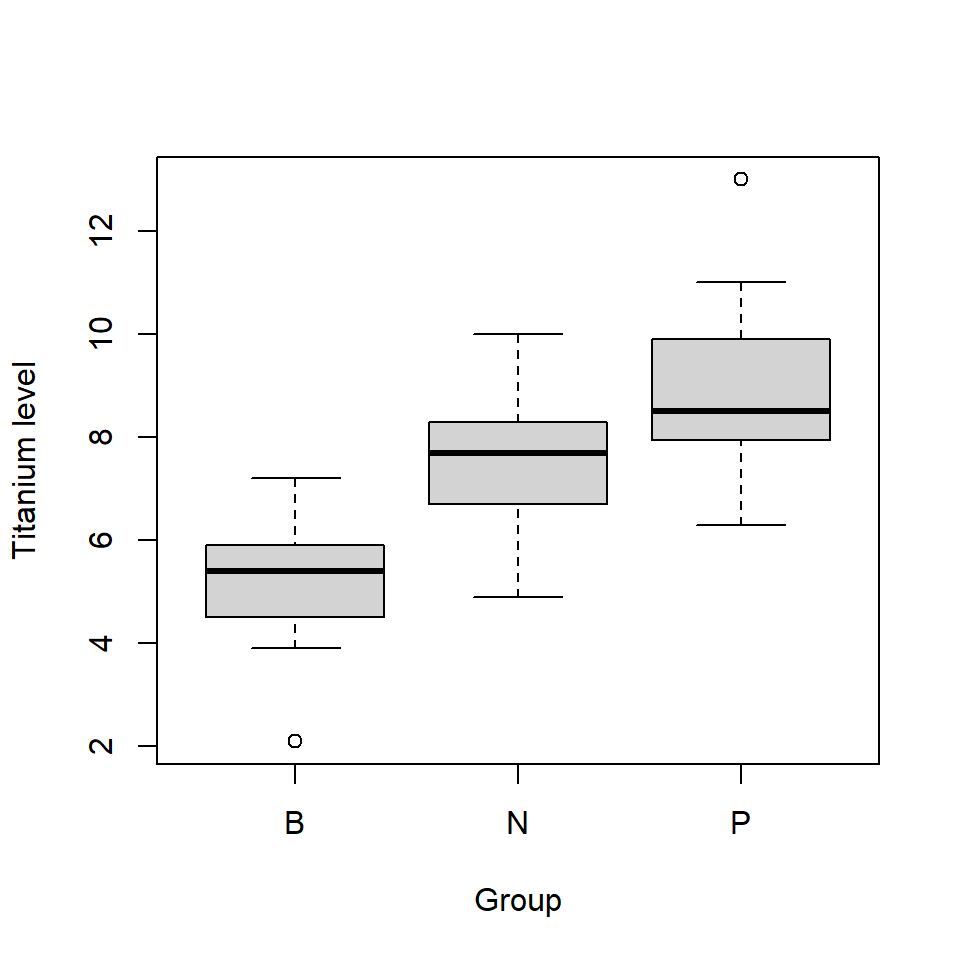
\includegraphics{IntroStats_files/figure-latex/plantbox-1} 

}

\caption{Distributions of titanium levels in three groups.}\label{fig:plantbox}
\end{figure}

There is a substantial overlap in the values between the three groups and so we will require formal methods to determine if the underlying groups means are the same or there is a real difference (beyond sampling variability). We could conduct a series of two sample \(t\) tests and compare B with N, B with P and N and P. However, when making a series of comparisons, we run the risk of drawing a false conclusion.

\hypertarget{type-i-and-type-ii-error}{%
\subsection{Type I and Type II error}\label{type-i-and-type-ii-error}}

When using a fixed significance level to draw a conclusion, the significance level, \(\alpha\) is the associated error rate - the probability of rejecting the null hypothesis when it is, in fact, true. For example, a significance level of 5\% (\(\alpha=0.05\)) means that there is a 5\% chance of rejecting the null hypothesis when it should not be rejected (e.g.~there is no difference between means). This is known as a Type I error. The converse error also exists, called a Type II error.

\begin{itemize}
\item
  \textbf{Type I error} - rejecting the null hypothesis when it is true (false positive)
\item
  \textbf{Type II error} - not rejecting the null hypothesis when it is false (false negative)
\end{itemize}

Table \ref{tab:type12} should help with understanding.

\begin{longtable}[]{@{}lll@{}}
\caption{\label{tab:type12} Possibilities for \(H_0\) and the decision based on test results.}\tabularnewline
\toprule
~Outcome of test & \(H_0\) True & \(H_0\) False\tabularnewline
\midrule
\endfirsthead
\toprule
~Outcome of test & \(H_0\) True & \(H_0\) False\tabularnewline
\midrule
\endhead
Reject \(H_0\) & Type I Error & Correct decision\tabularnewline
Fail to reject \(H_0\) & Correct decision & Type II Error\tabularnewline
\bottomrule
\end{longtable}

In comparing each pair of groups, there is a Type I error associated with each test and the Type I error compounds every time we do an additional test. The error rate over all possible pairwise comparisons is then no longer 5\% and increases the chance of drawing false conclusions. We come back to this later in the chapter but essentially what we need is one test that compares all group means simultaneously; we do this using one-way Analysis of Variance.

\hypertarget{analysis-of-variance-anova}{%
\section{ANalysis Of VAriance (ANOVA)}\label{analysis-of-variance-anova}}

We want to test for differences in means between three or more groups. The null hypothesis will be that the group means are the same and the alternative hypothesis will be that at least one mean is difference from at least one other mean.

\textbf{Example} The null hypotheses to compare the mean titanium levels in three groups, B, N and P is:

\[ H_0: \mu_{\textrm{B}} = \mu_{\textrm{N}} = \mu_{\textrm{P}} \]
The alternative hypothesis is usually specified as

\[H_1: \textrm{at least one mean is different from one of the other means}\]
because specifying all the options is rather long-winded, i.e.~\(\mu_{\textrm{B}} = \mu_{\textrm{N}} \ne \mu_{\textrm{P}}\) or
\(\mu_{\textrm{B}} \ne \mu_{\textrm{N}} = \mu_{\textrm{P}}\) or
\(\mu_{\textrm{B}} \ne \mu_{\textrm{P}} = \mu_{\textrm{N}}\) or
\(\mu_{\textrm{B}} \ne \mu_{\textrm{N}} \ne \mu_{\textrm{P}}\).

If \(H_0\) is true, we would expect the group means to be similar and any observed differences between the sample means is due to sampling variation only. However, detecting differences between group means depends on the variability associated with each group. If there are no differences between means (i.e.~the null hypothesis is true) then any differences between the group means are likely to be small compared with the within group variability (Figure \ref{fig:groupbox2}).

\begin{figure}

{\centering 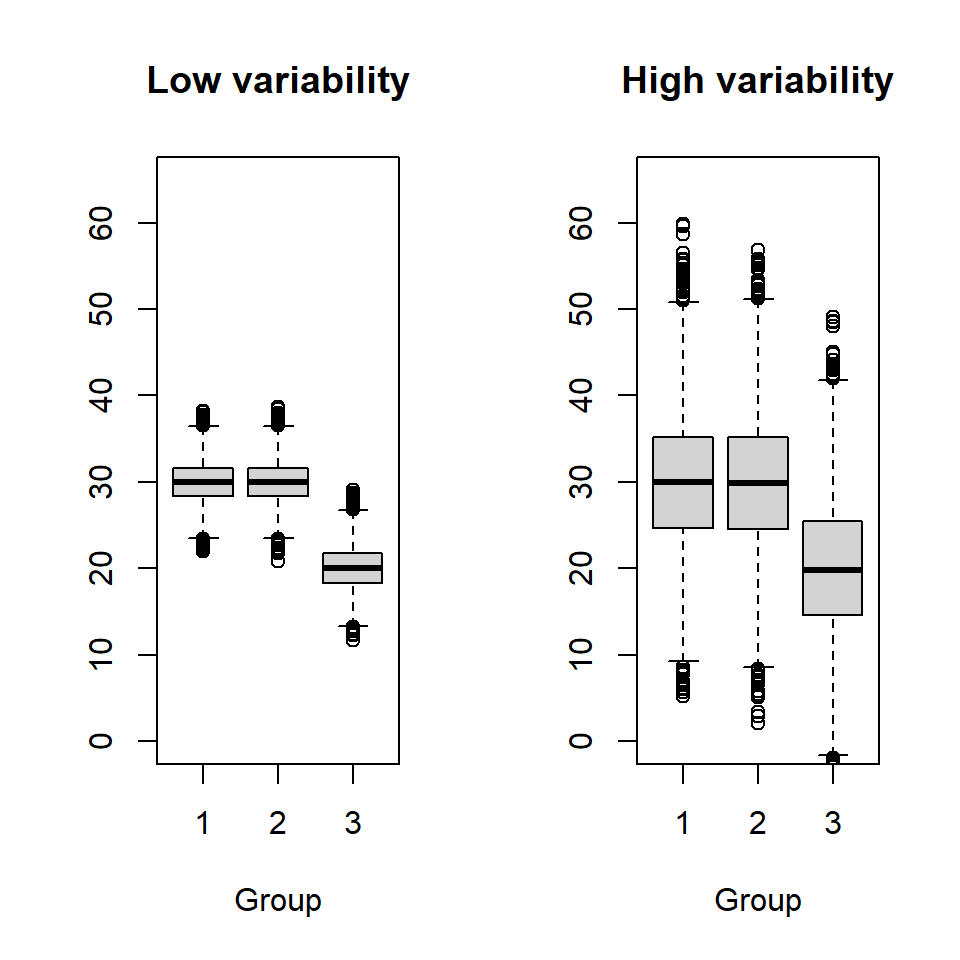
\includegraphics{IntroStats_files/figure-latex/groupbox2-1} 

}

\caption{Illustration of between and within group variability: the mean for groups 1 and 2 is 30 and the mean for group 3 is 20. The standard deviation is 2.5 on the left and 8 on the right.}\label{fig:groupbox2}
\end{figure}

The ANOVA procedure explicitly compares the `between' and `within' group variability to test \(H_0\). This is done using an \(F\) test statistic.

\hypertarget{f-test-statistic-for-anova}{%
\subsection{\texorpdfstring{\(F\) test statistic for ANOVA}{F test statistic for ANOVA}}\label{f-test-statistic-for-anova}}

The \(F\) test statistic for ANOVA is the ratio of the variability between groups (\(s_B^2\)) and the variability within groups (\(s_W^2\)):

\[f_0=\frac{s^2_B}{s^2_W}\]

The numerator, \(s^2_B\), represents the difference between each group mean and the overall mean (combined across groups). It will be large if there are large differences between the group means:

\[s^2_B=\frac{\sum_{i=1}^{k} n_i (\bar{x}_{i}-\bar{x}_{.})^2}{k-1}= \frac{SS_B}{k-1}\]

where

\begin{itemize}
\tightlist
\item
  \(k\) is the number of groups,
\item
  \(n_i\) is the sample size for group \(i\) and \(i=1, ..., k\),
\item
  \(\bar{x}_{i}\) is the sample mean for group \(i\), and
\item
  \(\bar{x}_{.}\) is the sample mean across all groups combined.
\end{itemize}

The denominator, \(s^2_W\), represents the variability within groups (via \(s^2_i\)) weighted by sample size within groups. It will be large if the data vary a great deal within groups (Figure \ref{fig:groupbox2}, right hand plot):

\[s^2_W = \frac{\sum_{i=1}^{k}(n_i-1)s_i^2}{n_{tot} - k} = \frac{SS_W}{n_{tot} - k}\]

\begin{itemize}
\tightlist
\item
  where \(s_i^2\) is the sample variance for group \(i\), and
\item
  \(n_{tot}\) is the total number of observations across all groups.
\end{itemize}

If \(H_0\) is true, \(f_0\) should be small - differences between means are small compared with the spread within groups. If \(H_0\) is false, \(f_0\) should be large - differences between means will be large compared to the spread within groups. Evidence against \(H_0\) is provided by values of \(f_0\) which would be unusually large when \(H_0\) is true. How large is large?

Deciding if a test statistic is typical under the null hypothesis, we compare the test statistic with a reference distribution; in this case, the \(F_{(df_1,df_2)}\) distribution, where \(df_1=k-1\) and \(df_2=n_{tot}-k\) is used. This distribution is also used to obtain an exact \(p\)-value for the test; we will use \texttt{R} for this in general (although there are tables where critical values can be looked up). Before looking at the \(F\) distribution, we examine how \(f_0\) is calculated. As with \(p\)-values, we will generally use R to calculate \(f_0\), however, it is useful to see how it is calculated and presented.

\hypertarget{calculating-an-anova-table}{%
\subsection{Calculating an ANOVA table}\label{calculating-an-anova-table}}

A convenient way to compile all the values for an \(F\) test statistic is to compile an ANOVA table (Table \ref{tab:anovatab}). The variability observed in the data is partitioned into the pattern, or signal, which can be explained by the different groups and then what is left over, called errors or residuals. Residuals will crop up again in chapter 13 when regression models are described. In fact with ANOVA, we are fitting a model, it is just that the explanatory variable is a nominal variable.

\begin{longtable}[]{@{}lllll@{}}
\caption{\label{tab:anovatab} Components of an ANOVA table.}\tabularnewline
\toprule
~Source of variation & df & Sum Sq & Mean Sq & \(F\) value\tabularnewline
\midrule
\endfirsthead
\toprule
~Source of variation & df & Sum Sq & Mean Sq & \(F\) value\tabularnewline
\midrule
\endhead
Between groups & \(k-1\) & \(SS_B\) & \(s_B^2\) & \(f_0\)\tabularnewline
Residuals & \(n_{tot}-k\) & \(SS_W\) & \(s_W^2\) &\tabularnewline
--------------- & -------------- & --------- & ---------- & --\tabularnewline
Total & \(n_{tot}-1\) & & &\tabularnewline
\bottomrule
\end{longtable}

The completed ANOVA table to test for differences between the mean titanium level in groups B, N and P is given in Table \ref{tab:anovatitanium}.

\begin{longtable}[]{@{}lllll@{}}
\caption{\label{tab:anovatitanium} ANOVA table testing for differences in mean titanium levels in plants grown in one of three growing mediums.}\tabularnewline
\toprule
~Source of variation & df & Sum Sq & Mean Sq & \(F\) value\tabularnewline
\midrule
\endfirsthead
\toprule
~Source of variation & df & Sum Sq & Mean Sq & \(F\) value\tabularnewline
\midrule
\endhead
Between groups & 2 & 118.60 & 59.30 & 28.31\tabularnewline
Residuals & 43 & 90.06 & 2.09 &\tabularnewline
--------------- & -------------- & --------- & ---------- & --\tabularnewline
Total & 45 & & &\tabularnewline
\bottomrule
\end{longtable}

To illustrate the calculations, the number of observations, sample means and standard deviations are required for each group and also these values overall groups (Table \ref{tab:plantsumtab}).

\begin{longtable}[]{@{}cccc@{}}
\caption{\label{tab:plantsumtab} Summary statistics of the titanium levels in plants.}\tabularnewline
\toprule
\begin{minipage}[b]{(\columnwidth - 3\tabcolsep) * \real{0.11}}\centering
GM\strut
\end{minipage} & \begin{minipage}[b]{(\columnwidth - 3\tabcolsep) * \real{0.07}}\centering
n\strut
\end{minipage} & \begin{minipage}[b]{(\columnwidth - 3\tabcolsep) * \real{0.10}}\centering
Mean\strut
\end{minipage} & \begin{minipage}[b]{(\columnwidth - 3\tabcolsep) * \real{0.11}}\centering
SD\strut
\end{minipage}\tabularnewline
\midrule
\endfirsthead
\toprule
\begin{minipage}[b]{(\columnwidth - 3\tabcolsep) * \real{0.11}}\centering
GM\strut
\end{minipage} & \begin{minipage}[b]{(\columnwidth - 3\tabcolsep) * \real{0.07}}\centering
n\strut
\end{minipage} & \begin{minipage}[b]{(\columnwidth - 3\tabcolsep) * \real{0.10}}\centering
Mean\strut
\end{minipage} & \begin{minipage}[b]{(\columnwidth - 3\tabcolsep) * \real{0.11}}\centering
SD\strut
\end{minipage}\tabularnewline
\midrule
\endhead
\begin{minipage}[t]{(\columnwidth - 3\tabcolsep) * \real{0.11}}\centering
B\strut
\end{minipage} & \begin{minipage}[t]{(\columnwidth - 3\tabcolsep) * \real{0.07}}\centering
13\strut
\end{minipage} & \begin{minipage}[t]{(\columnwidth - 3\tabcolsep) * \real{0.10}}\centering
5.1\strut
\end{minipage} & \begin{minipage}[t]{(\columnwidth - 3\tabcolsep) * \real{0.11}}\centering
1.318\strut
\end{minipage}\tabularnewline
\begin{minipage}[t]{(\columnwidth - 3\tabcolsep) * \real{0.11}}\centering
N\strut
\end{minipage} & \begin{minipage}[t]{(\columnwidth - 3\tabcolsep) * \real{0.07}}\centering
9\strut
\end{minipage} & \begin{minipage}[t]{(\columnwidth - 3\tabcolsep) * \real{0.10}}\centering
7.58\strut
\end{minipage} & \begin{minipage}[t]{(\columnwidth - 3\tabcolsep) * \real{0.11}}\centering
1.622\strut
\end{minipage}\tabularnewline
\begin{minipage}[t]{(\columnwidth - 3\tabcolsep) * \real{0.11}}\centering
P\strut
\end{minipage} & \begin{minipage}[t]{(\columnwidth - 3\tabcolsep) * \real{0.07}}\centering
24\strut
\end{minipage} & \begin{minipage}[t]{(\columnwidth - 3\tabcolsep) * \real{0.10}}\centering
8.85\strut
\end{minipage} & \begin{minipage}[t]{(\columnwidth - 3\tabcolsep) * \real{0.11}}\centering
1.447\strut
\end{minipage}\tabularnewline
\begin{minipage}[t]{(\columnwidth - 3\tabcolsep) * \real{0.11}}\centering
Total\strut
\end{minipage} & \begin{minipage}[t]{(\columnwidth - 3\tabcolsep) * \real{0.07}}\centering
46\strut
\end{minipage} & \begin{minipage}[t]{(\columnwidth - 3\tabcolsep) * \real{0.10}}\centering
7.54\strut
\end{minipage} & \begin{minipage}[t]{(\columnwidth - 3\tabcolsep) * \real{0.11}}\centering
2.153\strut
\end{minipage}\tabularnewline
\bottomrule
\end{longtable}

Each component of the table is calculated as follows:

\begin{equation}\label{}
\begin{split}
SS_B & = \sum_{i=1}^{k} n_i (\bar{x}_{i.}-\bar{x}_{..})^2 \\
& = 13(5.10 - 7.54)^2 + 9(7.58 - 7.54)^2 + 24(8.85 - 7.54)^2 \\
& = 118.60
\end{split}
\end{equation}

\[s^2_B = \frac{SS_B}{k-1} = \frac{118.60}{3-1} = 59.30 \]

\begin{equation}
\begin{split}
SS_W & = \sum_{i=1}^{k}(n_i-1)s_i^2 \\
& = (13-1)1.318^2 + (9-1)1.622^2 + (23-1)1.447^2 \\
& = 88.16
\end{split}
\end{equation}

\[s^2_W = \frac{SS_W}{n_{tot}-k} = \frac{90.06}{46 - 3} = 2.09\]
Finally,

\[f_0 = \frac{s^2_B}{s^2_W} = \frac{59.307}{2.09} = 28.31\]

Hence, the test statistic is 28.31. To decide whether this is large, we compare it to the \(F_{(df_1,df_2)}\) distribution.

\hypertarget{f-distribution}{%
\subsection{\texorpdfstring{\(F\) distribution}{F distribution}}\label{f-distribution}}

The \(F\) distribution (named in honour of R. A. Fisher) is a continuous distribution. It is defined by two parameters, \(F_{df_1,df_2}\), where,

\begin{itemize}
\tightlist
\item
  \(df_1 = k - 1\)
\item
  \(df_2 = n_{tot} - k\).
\end{itemize}

The \(F\) distribution can take on a variety of shapes but cannot have negative values. Figure \ref{fig:fdist} shows some examples of shapes and you can also explore the shape changes yourself in Figure \ref{fig:fshiny}.

\begin{figure}

{\centering 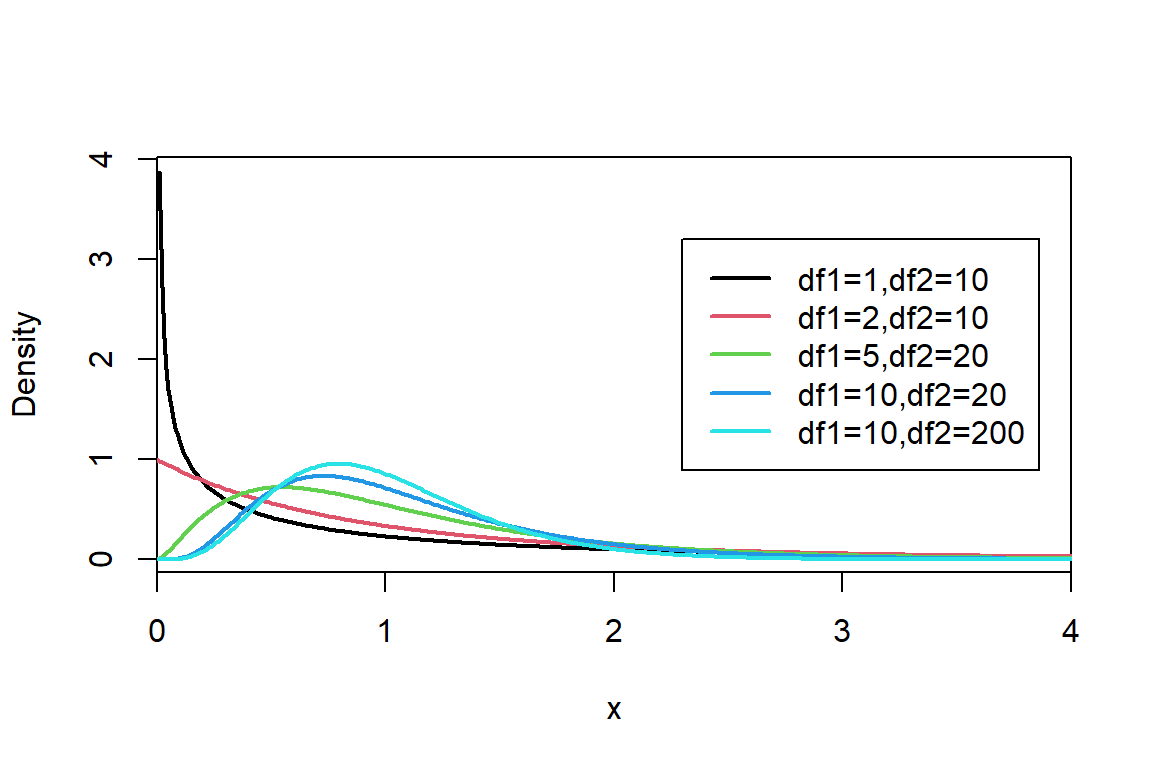
\includegraphics{IntroStats_files/figure-latex/fdist-1} 

}

\caption{The probability density function of $F_{df1,df2}$ distribution for different values of the parameters $df1$ and $df2$.}\label{fig:fdist}
\end{figure}



\begin{figure}

{\centering \href{https://moniquemackenzie.shinyapps.io/IntroStats_Fdistribution/}{\includegraphics{IntroStats_files/figure-latex/fshiny-1} }

}

\caption{Visualising the F-distribution. You can see a live version by clicking \href{https://moniquemackenzie.shinyapps.io/IntroStats_Fdistribution/}{here}}\label{fig:fshiny}
\end{figure}

In our example, \(df_1=2\) and \(df_2=43\) and this distribution is shown in Figure \ref{fig:fdist2and4}. We can see that the density (on the \(y\)-axis) at a value of about 6 on the \(x\)-axis is pretty much zero. Our test statistic is 28.31, hence the probability of obtaining a value as large and larger than this (i.e.~\(Pr(f \ge 28.31)\) where \(f \sim F_{2,43}\)) is going to be small; in fact the \(p\)-value is \(<0.0001\). This indicates that it is very unlikely to obtain a value as large, or larger, than 28.31 when the group means are the same. We reject \(H_0\) and have strong evidence that at least one of the group means is different to one of the other means.

\begin{figure}

{\centering 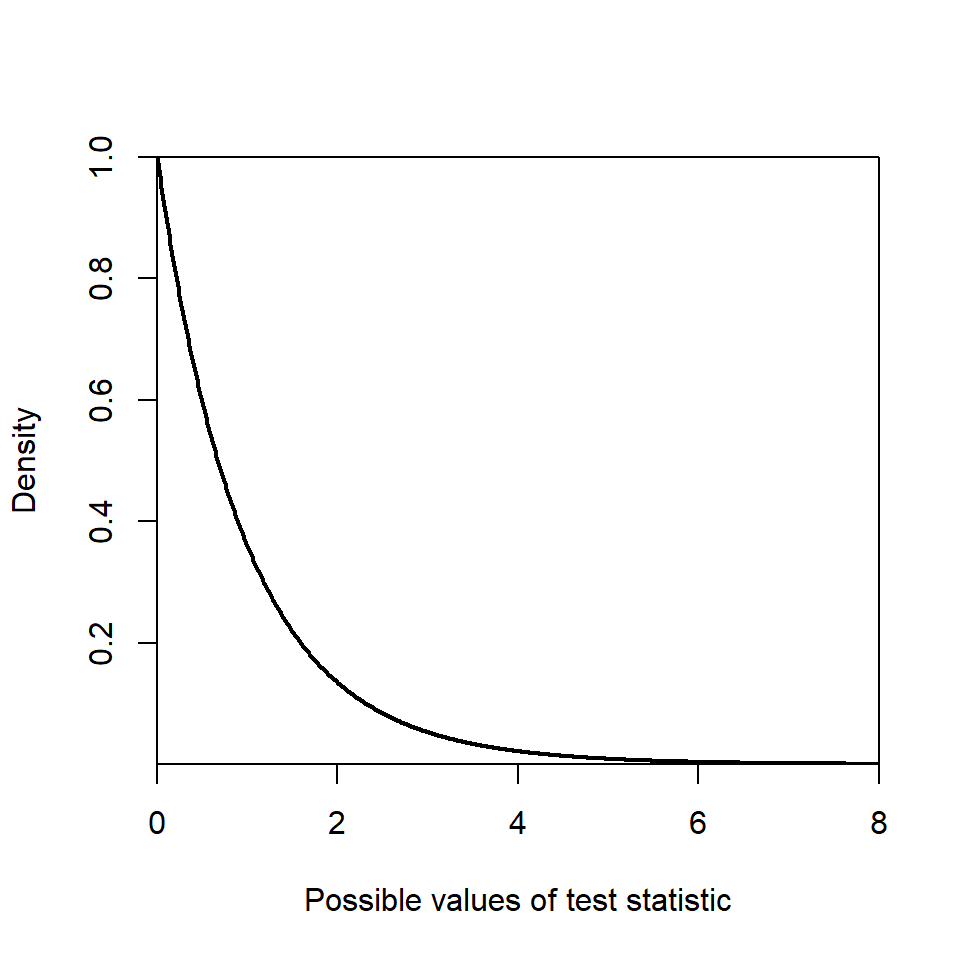
\includegraphics{IntroStats_files/figure-latex/fdist2and4-1} 

}

\caption{Reference distribution, $F_{2,43}$ distribution.}\label{fig:fdist2and4}
\end{figure}

\hypertarget{doing-this-in-r-16}{%
\subsection{Doing this in R}\label{doing-this-in-r-16}}

Fortunately R removes the hard work and does all the calculations, however, to make sense of the output created by the \texttt{aov} function, and create a neat ANOVA table, the \texttt{summary} function is used.

\begin{Shaded}
\begin{Highlighting}[]
\CommentTok{\# Fit ANOVA}
\NormalTok{plant.aov }\OtherTok{\textless{}{-}} \FunctionTok{aov}\NormalTok{(Ti }\SpecialCharTok{\textasciitilde{}}\NormalTok{ Group, }\AttributeTok{data=}\NormalTok{plant)}
\CommentTok{\# Display ANOVA table}
\FunctionTok{summary}\NormalTok{(plant.aov)}
\end{Highlighting}
\end{Shaded}

\begin{verbatim}
            Df Sum Sq Mean Sq F value   Pr(>F)    
Group        2 118.60   59.30   28.31 1.43e-08 ***
Residuals   43  90.06    2.09                     
---
Signif. codes:  0 '***' 0.001 '**' 0.01 '*' 0.05 '.' 0.1 ' ' 1
\end{verbatim}

The asterisks give a visual indication of the significance level; in this case the three asterisks (\texttt{***}) indicate that the \(p\)-value is between 0 and 0.001.

One thing to note is that the \(p\)-value is only associated with the upper tail. Hence, if we want to calculate the exact \(p\)-value, the upper tail has to be specified in the function to obtain the \(p\)-value, or indeed if we want to obtain a critical value.

\begin{Shaded}
\begin{Highlighting}[]
\CommentTok{\# Exact p{-}value}
\FunctionTok{pf}\NormalTok{(}\AttributeTok{q=}\FloatTok{28.31}\NormalTok{, }\AttributeTok{df1=}\DecValTok{2}\NormalTok{, }\AttributeTok{df2=}\DecValTok{43}\NormalTok{, }\AttributeTok{lower.tail=}\ConstantTok{FALSE}\NormalTok{)}
\end{Highlighting}
\end{Shaded}

\begin{verbatim}
[1] 1.429293e-08
\end{verbatim}

\begin{Shaded}
\begin{Highlighting}[]
\CommentTok{\# Critical value, testing at a significance level of 5\%}
\FunctionTok{qf}\NormalTok{(}\AttributeTok{p=}\FloatTok{0.05}\NormalTok{, }\AttributeTok{df1=}\DecValTok{2}\NormalTok{, }\AttributeTok{df2=}\DecValTok{43}\NormalTok{, }\AttributeTok{lower.tail=}\ConstantTok{FALSE}\NormalTok{)}
\end{Highlighting}
\end{Shaded}

\begin{verbatim}
[1] 3.21448
\end{verbatim}

The critical value, testing at a significance level of 5\%, is 3.21 - our test statistic (\(f_0\)=28.31) is much larger than this, hence, leading us to the same conclusion.

\textbf{Q9.1} A consumer organisation was interested in comparing the price of petrol (pence per litre) in four different locations classified as city, motorway, rural and town. Prices at ten petrol stations, selected at random for the four locations, were recorded; a summary of the results are provided below.

\begin{longtable}[]{@{}cccc@{}}
\toprule
\begin{minipage}[b]{(\columnwidth - 3\tabcolsep) * \real{0.15}}\centering
Location\strut
\end{minipage} & \begin{minipage}[b]{(\columnwidth - 3\tabcolsep) * \real{0.07}}\centering
n\strut
\end{minipage} & \begin{minipage}[b]{(\columnwidth - 3\tabcolsep) * \real{0.11}}\centering
Mean\strut
\end{minipage} & \begin{minipage}[b]{(\columnwidth - 3\tabcolsep) * \real{0.11}}\centering
SD\strut
\end{minipage}\tabularnewline
\midrule
\endhead
\begin{minipage}[t]{(\columnwidth - 3\tabcolsep) * \real{0.15}}\centering
City\strut
\end{minipage} & \begin{minipage}[t]{(\columnwidth - 3\tabcolsep) * \real{0.07}}\centering
10\strut
\end{minipage} & \begin{minipage}[t]{(\columnwidth - 3\tabcolsep) * \real{0.11}}\centering
135.4\strut
\end{minipage} & \begin{minipage}[t]{(\columnwidth - 3\tabcolsep) * \real{0.11}}\centering
5.52\strut
\end{minipage}\tabularnewline
\begin{minipage}[t]{(\columnwidth - 3\tabcolsep) * \real{0.15}}\centering
Motorway\strut
\end{minipage} & \begin{minipage}[t]{(\columnwidth - 3\tabcolsep) * \real{0.07}}\centering
10\strut
\end{minipage} & \begin{minipage}[t]{(\columnwidth - 3\tabcolsep) * \real{0.11}}\centering
143.6\strut
\end{minipage} & \begin{minipage}[t]{(\columnwidth - 3\tabcolsep) * \real{0.11}}\centering
3.84\strut
\end{minipage}\tabularnewline
\begin{minipage}[t]{(\columnwidth - 3\tabcolsep) * \real{0.15}}\centering
Rural\strut
\end{minipage} & \begin{minipage}[t]{(\columnwidth - 3\tabcolsep) * \real{0.07}}\centering
10\strut
\end{minipage} & \begin{minipage}[t]{(\columnwidth - 3\tabcolsep) * \real{0.11}}\centering
140.4\strut
\end{minipage} & \begin{minipage}[t]{(\columnwidth - 3\tabcolsep) * \real{0.11}}\centering
6.43\strut
\end{minipage}\tabularnewline
\begin{minipage}[t]{(\columnwidth - 3\tabcolsep) * \real{0.15}}\centering
Town\strut
\end{minipage} & \begin{minipage}[t]{(\columnwidth - 3\tabcolsep) * \real{0.07}}\centering
10\strut
\end{minipage} & \begin{minipage}[t]{(\columnwidth - 3\tabcolsep) * \real{0.11}}\centering
133\strut
\end{minipage} & \begin{minipage}[t]{(\columnwidth - 3\tabcolsep) * \real{0.11}}\centering
7\strut
\end{minipage}\tabularnewline
\begin{minipage}[t]{(\columnwidth - 3\tabcolsep) * \real{0.15}}\centering
Total\strut
\end{minipage} & \begin{minipage}[t]{(\columnwidth - 3\tabcolsep) * \real{0.07}}\centering
40\strut
\end{minipage} & \begin{minipage}[t]{(\columnwidth - 3\tabcolsep) * \real{0.11}}\centering
138.1\strut
\end{minipage} & \begin{minipage}[t]{(\columnwidth - 3\tabcolsep) * \real{0.11}}\centering
7\strut
\end{minipage}\tabularnewline
\bottomrule
\end{longtable}

\textbf{a.} Describe the null and alternative hypotheses to be tested.

\textbf{b.} Complete the ANOVA table to calculate the \(F\) test statistic.

\textbf{c.} A critical value, testing at a significance level of 5\%, for the reference \(F\) distribution is given below. What do you conclude regarding the mean prices between locations?

\begin{Shaded}
\begin{Highlighting}[]
\FunctionTok{qf}\NormalTok{(}\AttributeTok{p=}\FloatTok{0.05}\NormalTok{, }\AttributeTok{df1=}\DecValTok{3}\NormalTok{, }\AttributeTok{df2=}\DecValTok{36}\NormalTok{, }\AttributeTok{lower.tail=}\ConstantTok{FALSE}\NormalTok{)}
\end{Highlighting}
\end{Shaded}

\begin{verbatim}
[1] 2.866266
\end{verbatim}

\hypertarget{assumptions}{%
\subsection{Assumptions}\label{assumptions}}

In order for the \(F\) test results to be valid, we need the following assumptions to be met:

\begin{itemize}
\tightlist
\item
  Independence: the data are sampled independently,
\item
  Normality: the data for each group appears to have come from a Normal distribution,
\item
  Constant spread: the underlying standard deviations for each group appear to be equal.
\end{itemize}

ANOVA is reasonably robust to departures from the `constant spread' and `Normality' assumptions, however, the `independence' assumption is critical for valid results. As a conservative rule of thumb, ANOVA should give reliable results if the largest standard deviation of the groups is no larger than twice the smallest standard deviation of the groups.

\textbf{Example} We can check these assumptions for the ANOVA we have conducted on the plant data. Within each group, different plants were measured for titanium levels and without knowing further details of the data collection, we assume the values are independent. The other assumptions can be tested more formally.

\textbf{Checking constant spread}

Table 9.4 indicates that the standard deviations are similar in each group based on the rule of thumb - the smallest is 1.318 and the largest is 1.622. Levene's test provides a formal test. The null hypothesis is that the population variances for each group are equal (called homogeneity of variances, or homoscedasticity); for example

\[H_0: \sigma_B^2 = \sigma_N^2 = \sigma_P^2 \]
The test statistic is compared to an \(F_{df_1,df_2}\) distribution (i.e.~the same reference distribution as for ANOVA) and we use R to illustrate this. The \texttt{car} \citep{Fox2019} library is required for Levene's test.

\begin{Shaded}
\begin{Highlighting}[]
\FunctionTok{library}\NormalTok{(car)}
\FunctionTok{leveneTest}\NormalTok{(Ti }\SpecialCharTok{\textasciitilde{}}\NormalTok{ Group, }\AttributeTok{data=}\NormalTok{plant)}
\end{Highlighting}
\end{Shaded}

\begin{verbatim}
Levene's Test for Homogeneity of Variance (center = median)
      Df F value Pr(>F)
group  2  0.1852 0.8316
      43               
\end{verbatim}

The \(p\)-value is interpreted in the same way as for other hypothesis test - in this example, the \(p\)-value is large and so we cannot reject the null hypothesis and conclude that the variances are the same.

\textbf{Checking normality}

To check whether the data are normally distributed we can examine the observations (as in Figure \ref{fig:plantbox}) or look at the residuals (differences between the observations and the values created when fitting the model). The residuals should lie on a straight line if they are normally distributed. (There will be more on residuals in a later chapter.)

\begin{Shaded}
\begin{Highlighting}[]
\CommentTok{\# Plot a normal QQ plot}
\FunctionTok{qqnorm}\NormalTok{(plant.aov}\SpecialCharTok{$}\NormalTok{residuals)}
\CommentTok{\# Add a line to the plot}
\FunctionTok{qqline}\NormalTok{(plant.aov}\SpecialCharTok{$}\NormalTok{residuals)}
\end{Highlighting}
\end{Shaded}

\begin{figure}

{\centering 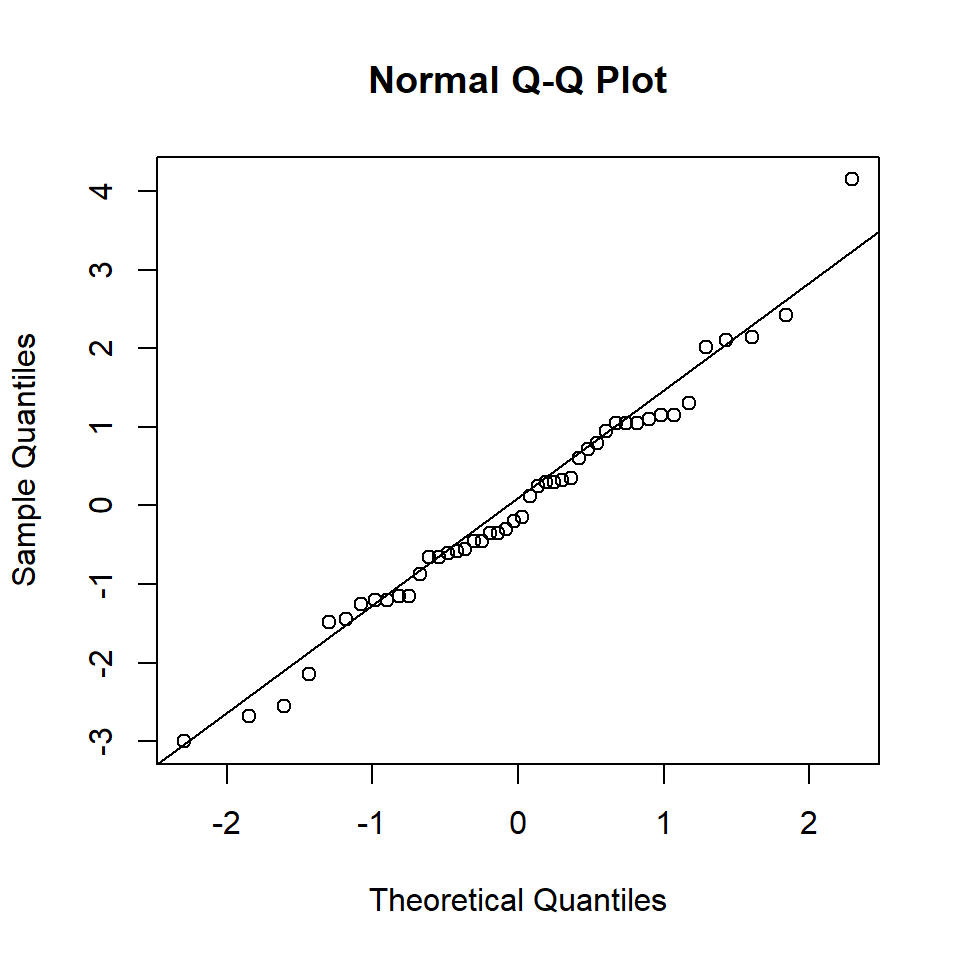
\includegraphics{IntroStats_files/figure-latex/qqnorm1-1} 

}

\caption{Quantile-quantile plot of residuals.}\label{fig:qqnorm1}
\end{figure}

Figure \ref{fig:qqnorm1} indicates that the residuals lie roughly on a straight line. To formally check, we can undertake a Shapiro-Wilk test. The null hypothesis for this test is that the data come from a normally distributed population.

\begin{Shaded}
\begin{Highlighting}[]
\FunctionTok{shapiro.test}\NormalTok{(plant.aov}\SpecialCharTok{$}\NormalTok{residuals)}
\end{Highlighting}
\end{Shaded}

\begin{verbatim}
    Shapiro-Wilk normality test

data:  plant.aov$residuals
W = 0.98038, p-value = 0.6216
\end{verbatim}

We see from the results that the \(p\)-value is large (0.62), thus, there is no evidence to reject the null hypothesis and we can conclude that the data are normally distributed.

All the assumptions have been checked (as far as possible) and are valid for these plant data. Thus, we can move on with the analysis to try and determine where differences lie.

\hypertarget{identifying-differences-and-more-on-multiple-comparisons}{%
\section{Identifying differences (and more on multiple comparisons)}\label{identifying-differences-and-more-on-multiple-comparisons}}

ANOVA identifies whether, or not, a difference exists between at least one pair of group means. If a difference exists, the next stage is to identify which pairs of groups are different and how large any differences might be. There will be three pairwise comparisons for three groups (B-N, B-P and N-P) but the number soon increases with more groups; the number is given by for \(k\) groups:

\[\textrm{number of pairwise comparisons} = \frac{k!}{(k-2)!2!}\]

We could build 95\% confidence intervals for each pairwise comparison but each has a Type I error rate of 5\%; these errors compound and so we can adjust the error rate so that the overall, or \textbf{family wise}, error rate is 5\%. There are various methods of making this adjustment and here we look at three methods; Bonferroni correction, Sidak adjustment and Tukey's Honest Significance Differences.

\textbf{Q9.2} If there are four groups to be compared (as in Q9.1), how many pairwise comparisons can be made?

\hypertarget{bonferroni-correction}{%
\subsection{Bonferroni correction}\label{bonferroni-correction}}

This is a simple method; we calculate a new threshold \(p\)-value by dividing the desired Type I error rate (overall comparisons), by the number of comparisons:

\[\alpha_{adj} = \frac{\alpha}{c}\]
where

\begin{itemize}
\tightlist
\item
  \(\alpha_{adj}\) is the new threshold,
\item
  \(\alpha\) is the desired Type I error collectively (family error rate) and
\item
  \(c\) is the number of comparisons.
\end{itemize}

\textbf{Example} We want to conduct a series of 5 two sample \(t\) tests with a desired overall error rate of 5\%. The adjusted error rate is thus, \(\alpha_{adj} = 0.05/5 = 0.01\) and so rather than accept a result as significant if the probability is below 0.05, we accept it as significant if the \(p\)-value for each test is below 0.01.

This method is considered to be `conservative' with respect to the family wise error rate, particularly if there are a large number of tests, or comparisons. This correction comes at the cost of increasing the Type II error.

\hypertarget{sidak-adjustment}{%
\subsection{Sidak adjustment}\label{sidak-adjustment}}

The Sidak adjustment for the new threshold \(p\)-value is calculated from:

\[\alpha_{adj} = 1 - (1-\alpha)^{\frac{1}{c}}\]
\textbf{Example} We have a control treatment and plan to compare it against 3 different treatments and require an overall Type I error of 5\%:

\[\alpha_{adj} = 1 - (1 - 0.05)^{\frac{1}{3}}=0.01695\]
Therefore, a \(p\)-value \textless{} 0.01695 is required to conclude a significant result for each comparison.

\hypertarget{tukeys-honest-significant-difference-hsd}{%
\subsection{Tukey's Honest Significant Difference (HSD)}\label{tukeys-honest-significant-difference-hsd}}

This method is similar to creating confidence intervals for differences between two means but modifies the standard error and multiplier resulting in wider confidence intervals. We can then check to see if zero is contained within each CI to determine whether any pair of group means are significantly different with a family wise error rate of \(\alpha\).

\textbf{Example} We return to the data of titanium levels in plants grown in three different types of growing medium; previously we found that a difference does exist. We calculate Tukey's HSD for the pairwise comparisons to decide where any differences might lie (Table \ref{tab:tukeydif}).

\begin{longtable}[]{@{}ccccc@{}}
\caption{\label{tab:tukeydif} Differences and confidence intervals obtained using Tukey's HSD; the columns are described below.}\tabularnewline
\toprule
\begin{minipage}[b]{(\columnwidth - 4\tabcolsep) * \real{0.14}}\centering
~\strut
\end{minipage} & \begin{minipage}[b]{(\columnwidth - 4\tabcolsep) * \real{0.11}}\centering
diff\strut
\end{minipage} & \begin{minipage}[b]{(\columnwidth - 4\tabcolsep) * \real{0.14}}\centering
lwr\strut
\end{minipage} & \begin{minipage}[b]{(\columnwidth - 4\tabcolsep) * \real{0.11}}\centering
upr\strut
\end{minipage} & \begin{minipage}[b]{(\columnwidth - 4\tabcolsep) * \real{0.17}}\centering
p adj\strut
\end{minipage}\tabularnewline
\midrule
\endfirsthead
\toprule
\begin{minipage}[b]{(\columnwidth - 4\tabcolsep) * \real{0.14}}\centering
~\strut
\end{minipage} & \begin{minipage}[b]{(\columnwidth - 4\tabcolsep) * \real{0.11}}\centering
diff\strut
\end{minipage} & \begin{minipage}[b]{(\columnwidth - 4\tabcolsep) * \real{0.14}}\centering
lwr\strut
\end{minipage} & \begin{minipage}[b]{(\columnwidth - 4\tabcolsep) * \real{0.11}}\centering
upr\strut
\end{minipage} & \begin{minipage}[b]{(\columnwidth - 4\tabcolsep) * \real{0.17}}\centering
p adj\strut
\end{minipage}\tabularnewline
\midrule
\endhead
\begin{minipage}[t]{(\columnwidth - 4\tabcolsep) * \real{0.14}}\centering
\textbf{N-B}\strut
\end{minipage} & \begin{minipage}[t]{(\columnwidth - 4\tabcolsep) * \real{0.11}}\centering
2.478\strut
\end{minipage} & \begin{minipage}[t]{(\columnwidth - 4\tabcolsep) * \real{0.14}}\centering
0.9545\strut
\end{minipage} & \begin{minipage}[t]{(\columnwidth - 4\tabcolsep) * \real{0.11}}\centering
4.001\strut
\end{minipage} & \begin{minipage}[t]{(\columnwidth - 4\tabcolsep) * \real{0.17}}\centering
0.0008236\strut
\end{minipage}\tabularnewline
\begin{minipage}[t]{(\columnwidth - 4\tabcolsep) * \real{0.14}}\centering
\textbf{P-B}\strut
\end{minipage} & \begin{minipage}[t]{(\columnwidth - 4\tabcolsep) * \real{0.11}}\centering
3.75\strut
\end{minipage} & \begin{minipage}[t]{(\columnwidth - 4\tabcolsep) * \real{0.14}}\centering
2.54\strut
\end{minipage} & \begin{minipage}[t]{(\columnwidth - 4\tabcolsep) * \real{0.11}}\centering
4.96\strut
\end{minipage} & \begin{minipage}[t]{(\columnwidth - 4\tabcolsep) * \real{0.17}}\centering
6.734e-09\strut
\end{minipage}\tabularnewline
\begin{minipage}[t]{(\columnwidth - 4\tabcolsep) * \real{0.14}}\centering
\textbf{P-N}\strut
\end{minipage} & \begin{minipage}[t]{(\columnwidth - 4\tabcolsep) * \real{0.11}}\centering
1.272\strut
\end{minipage} & \begin{minipage}[t]{(\columnwidth - 4\tabcolsep) * \real{0.14}}\centering
-0.1009\strut
\end{minipage} & \begin{minipage}[t]{(\columnwidth - 4\tabcolsep) * \real{0.11}}\centering
2.645\strut
\end{minipage} & \begin{minipage}[t]{(\columnwidth - 4\tabcolsep) * \real{0.17}}\centering
0.07432\strut
\end{minipage}\tabularnewline
\bottomrule
\end{longtable}

\begin{itemize}
\item
  the first column indicates the two groups being compared,
\item
  `diff' is the point estimate of the difference in means between the two groups,
\item
  `lwr' and `upr' are the lower and upper bounds, respectively, of the confidence interval for the difference taking into account the multiple comparisons, and
\item
  `\(p\) adj' is the \(p\)-value evaluating the null hypothesis that the difference between the means of the populations is zero taking into account the number of multiple comparisons.
\end{itemize}

In this case, one confidence interval contains zero (i.e.~P-N); on average the mean titanium level in group P is between -0.1 units lower to 2.65 units higher than group N. An interval containing zero indicates that zero is a plausible value for the difference in means, thus the means for these two groups are not significantly different.

The other intervals are significantly different - the interval does not contain zero. The mean titanium level in N is significantly higher than B - on average 0.95 to 4.00 units higher (95\% confidence). Also, the level in P is significantly higher than in B - on average 2.54 to 4.96 units higher (95\% confidence)

As a comparison, Table \ref{tab:normalCI} shows that standard 95\% confidence intervals for each of the difference in means are slightly narrower than the confidence intervals obtained using Tukey's HSD (Table 9.5).

\begin{longtable}[]{@{}ccc@{}}
\caption{\label{tab:normalCI} Standard 95\% confidence intervals for each pairwise comparison.}\tabularnewline
\toprule
\begin{minipage}[b]{(\columnwidth - 2\tabcolsep) * \real{0.11}}\centering
Group\strut
\end{minipage} & \begin{minipage}[b]{(\columnwidth - 2\tabcolsep) * \real{0.15}}\centering
lwr\strut
\end{minipage} & \begin{minipage}[b]{(\columnwidth - 2\tabcolsep) * \real{0.11}}\centering
upr\strut
\end{minipage}\tabularnewline
\midrule
\endfirsthead
\toprule
\begin{minipage}[b]{(\columnwidth - 2\tabcolsep) * \real{0.11}}\centering
Group\strut
\end{minipage} & \begin{minipage}[b]{(\columnwidth - 2\tabcolsep) * \real{0.15}}\centering
lwr\strut
\end{minipage} & \begin{minipage}[b]{(\columnwidth - 2\tabcolsep) * \real{0.11}}\centering
upr\strut
\end{minipage}\tabularnewline
\midrule
\endhead
\begin{minipage}[t]{(\columnwidth - 2\tabcolsep) * \real{0.11}}\centering
N-B\strut
\end{minipage} & \begin{minipage}[t]{(\columnwidth - 2\tabcolsep) * \real{0.15}}\centering
1.086\strut
\end{minipage} & \begin{minipage}[t]{(\columnwidth - 2\tabcolsep) * \real{0.11}}\centering
3.87\strut
\end{minipage}\tabularnewline
\begin{minipage}[t]{(\columnwidth - 2\tabcolsep) * \real{0.11}}\centering
P-B\strut
\end{minipage} & \begin{minipage}[t]{(\columnwidth - 2\tabcolsep) * \real{0.15}}\centering
2.785\strut
\end{minipage} & \begin{minipage}[t]{(\columnwidth - 2\tabcolsep) * \real{0.11}}\centering
4.715\strut
\end{minipage}\tabularnewline
\begin{minipage}[t]{(\columnwidth - 2\tabcolsep) * \real{0.11}}\centering
P-N\strut
\end{minipage} & \begin{minipage}[t]{(\columnwidth - 2\tabcolsep) * \real{0.15}}\centering
-0.05809\strut
\end{minipage} & \begin{minipage}[t]{(\columnwidth - 2\tabcolsep) * \real{0.11}}\centering
2.603\strut
\end{minipage}\tabularnewline
\bottomrule
\end{longtable}

\hypertarget{doing-this-in-r-17}{%
\subsubsection{Doing this in R}\label{doing-this-in-r-17}}

\begin{Shaded}
\begin{Highlighting}[]
\CommentTok{\# Create ANOVA object}
\NormalTok{plant.aov }\OtherTok{\textless{}{-}} \FunctionTok{aov}\NormalTok{(Ti }\SpecialCharTok{\textasciitilde{}}\NormalTok{ Group, }\AttributeTok{data=}\NormalTok{plant)}
\CommentTok{\# Tukeys HSD}
\FunctionTok{TukeyHSD}\NormalTok{(plant.aov)}
\end{Highlighting}
\end{Shaded}

\begin{verbatim}
  Tukey multiple comparisons of means
    95% family-wise confidence level

Fit: aov(formula = Ti ~ Group, data = plant)

$Group
        diff        lwr      upr     p adj
N-B 2.477778  0.9544691 4.001086 0.0008236
P-B 3.750000  2.5402571 4.959743 0.0000000
P-N 1.272222 -0.1008697 2.645314 0.0743237
\end{verbatim}

These intervals can be displayed with a helpful dashed line allowing confidence intervals containing zero to be easily identified:

\begin{Shaded}
\begin{Highlighting}[]
\CommentTok{\# Plot Tukeys HSD}
\FunctionTok{plot}\NormalTok{(}\FunctionTok{TukeyHSD}\NormalTok{(plant.aov))}
\end{Highlighting}
\end{Shaded}

\begin{figure}

{\centering 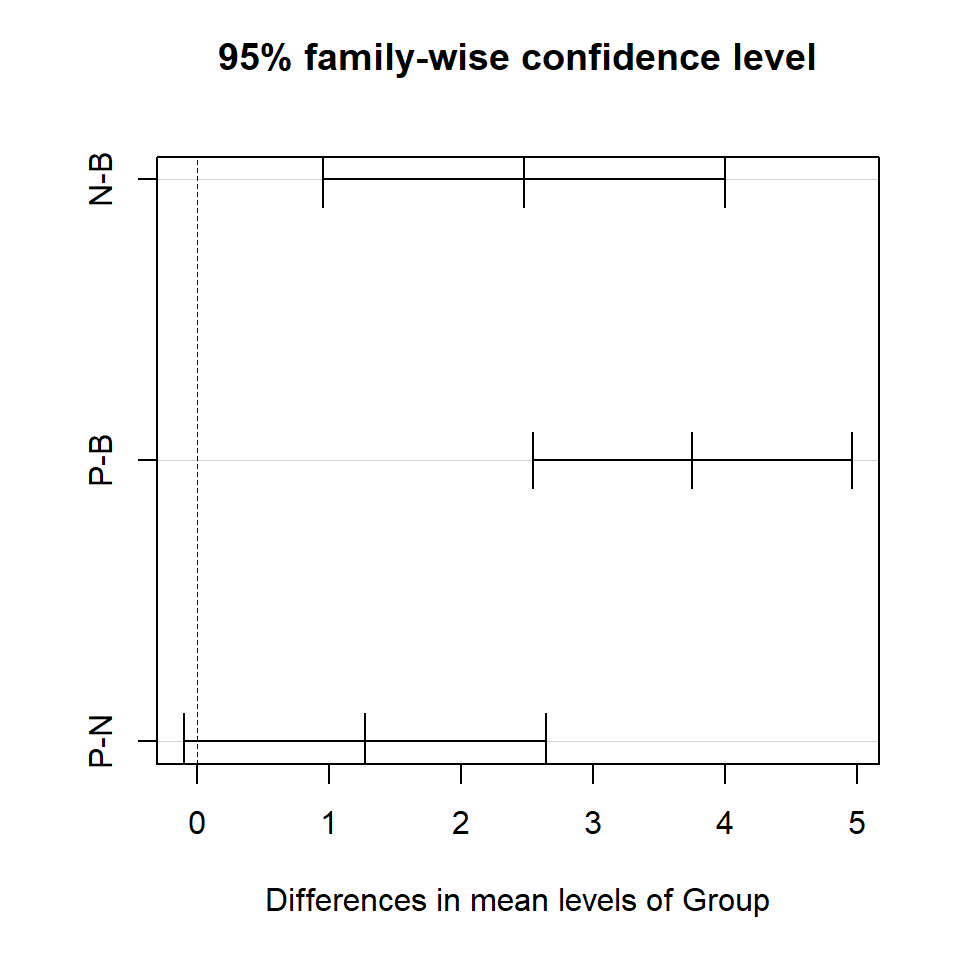
\includegraphics{IntroStats_files/figure-latex/unnamed-chunk-92-1} 

}

\caption{Comparison of titanium levels in groups B, N and P. The horizontal black lines indicate Tukey's HSD confidence interval for the pairwise comparison. The dashed line means it is easy to identify CI that include zero.}\label{fig:unnamed-chunk-92}
\end{figure}

\textbf{Q9.3} The following are Tukey's HSD comparing the petrol prices for four different locations.

\begin{Shaded}
\begin{Highlighting}[]
\FunctionTok{TukeyHSD}\NormalTok{(}\FunctionTok{aov}\NormalTok{(prices }\SpecialCharTok{\textasciitilde{}}\NormalTok{ location, }\AttributeTok{data=}\NormalTok{petrol))}
\end{Highlighting}
\end{Shaded}

\begin{verbatim}
  Tukey multiple comparisons of means
    95% family-wise confidence level

Fit: aov(formula = prices ~ location, data = petrol)

$location
                     diff        lwr        upr     p adj
Motorway-City    8.201950   1.191987 15.2119125 0.0164806
Rural-City       5.075935  -1.934027 12.0858982 0.2258147
Town-City       -2.408140  -9.418102  4.6018231 0.7915806
Rural-Motorway  -3.126014 -10.135977  3.8839485 0.6301923
Town-Motorway  -10.610089 -17.620052 -3.6001266 0.0013224
Town-Rural      -7.484075 -14.494038 -0.4741123 0.0326058
\end{verbatim}

\textbf{a.} Which locations are significantly different and which are not, testing at a significance level of 5\%?

\textbf{b.} Which two locations have the largest difference in means?

\hypertarget{multiple-comparison-controversy}{%
\subsection{Multiple comparison controversy}\label{multiple-comparison-controversy}}

In making adjustments when performing multiple comparisons, we are trading one error for another; we control a Type I error at the cost of a Type II error. For example, when making multiple comparisons, the adjustments reduce the threshold probability level used to determine significance. This means that we won't make many Type I errors, but Type II errors could be large. This relates to a concept called power, which is covered in chapter \ref{power}.

The choice of whether, or not, to make any adjustment is not straightforward and is generally context specific:

\begin{itemize}
\tightlist
\item
  sometimes people think adjustments should be made because they are really worried about Type I errors/false positives (e.g.~concluding a treatment is effective when it isn't)
\item
  sometimes making a Type II error/false negative could be concerning (e.g.~when exploring new cancer drugs a promising drug might be missed).
\end{itemize}

\hypertarget{alternative-tests-to-anova}{%
\section{Alternative tests to ANOVA}\label{alternative-tests-to-anova}}

If the data do not fulfill the test assumptions of normality and constant spread (or equal standard deviations), alternative tests are available and two are briefly described below. Although some assumptions can be relaxed with these tests, other assumptions can not.

If the data are not normally distributed, the Kruskal-Wallis test can be used as a non-parametric alternative to ANOVA; it can be thought of as a multi-level version of the Mann-Whitney test (chapter \ref{hypothtests}). However, this test does still assume that the groups have the same standard deviation. This test uses ranks and the null hypothesis is that the mean ranks of the groups is the same. The test statistic follows a \(\chi^2\) (chi-square) distribution which is indexed by one parameter, the degrees of freedom; this distribution is discussed in chapter \ref{tableofcounts}.

If the groups do not have similar standard deviations (heteroscedastic), an adaptation to ANOVA, called Welch's ANOVA, can be used, although this still requires that the data are normally distributed.

\hypertarget{doing-this-in-r-18}{%
\subsection{Doing this in R}\label{doing-this-in-r-18}}

The Kruskal\_Wallis test is performed with the \texttt{kruskal.test} function:

\begin{Shaded}
\begin{Highlighting}[]
\FunctionTok{kruskal.test}\NormalTok{(Ti }\SpecialCharTok{\textasciitilde{}}\NormalTok{ Group, }\AttributeTok{data=}\NormalTok{plant)}
\end{Highlighting}
\end{Shaded}

\begin{verbatim}
    Kruskal-Wallis rank sum test

data:  Ti by Group
Kruskal-Wallis chi-squared = 26.286, df = 2, p-value = 1.959e-06
\end{verbatim}

The \(p\)-value is interpreted in the same way; here it is very small, providing evidence to reject the null hypothesis. There is also a function which provides multiple comparisons after the Kruskal-Wallis test \citep{Siegel&Castellan1988}; this requires the \texttt{pgirmess} library \citep{R-pgirmess}. It identifies differences between groups depending on the specified significance level (0.05 by default).

\begin{Shaded}
\begin{Highlighting}[]
\FunctionTok{library}\NormalTok{(pgirmess)}
\FunctionTok{kruskalmc}\NormalTok{(Ti }\SpecialCharTok{\textasciitilde{}}\NormalTok{ Group, }\AttributeTok{data=}\NormalTok{plant)}
\end{Highlighting}
\end{Shaded}

\begin{verbatim}
Multiple comparison test after Kruskal-Wallis 
p.value: 0.05 
Comparisons
      obs.dif critical.dif difference
B-N 15.085470     13.93401       TRUE
B-P 23.682692     11.06576       TRUE
N-P  8.597222     12.55995      FALSE
\end{verbatim}

Welch's ANOVA is performed using \texttt{welch.test} which is in the \texttt{onewaytests} library \citep{R-onewaytests} (this is not part of the base libraries and so will need to be installed). Again it gives helpful output.

\begin{Shaded}
\begin{Highlighting}[]
\FunctionTok{library}\NormalTok{(onewaytests)}
\FunctionTok{welch.test}\NormalTok{(Ti }\SpecialCharTok{\textasciitilde{}}\NormalTok{ Group, }\AttributeTok{data=}\NormalTok{plant)}
\end{Highlighting}
\end{Shaded}

\begin{verbatim}
  Welch's Heteroscedastic F Test (alpha = 0.05) 
------------------------------------------------------------- 
  data : Ti and Group 

  statistic  : 30.83309 
  num df     : 2 
  denom df   : 19.47308 
  p.value    : 9.232681e-07 

  Result     : Difference is statistically significant. 
------------------------------------------------------------- 
\end{verbatim}

\hypertarget{SUManova}{%
\section{Summary}\label{SUManova}}

Analysis of variance, the procedure for comparing differences in means for more than two groups is a frequently used procedure. Technically we have described here, a one-way ANOVA because data are divided by only one factor, i.e.~the different groups. Not covered here is a two-way ANOVA where two factors can be taken into account. As with any statistical test, there are underlying assumptions which need to be met for the results to be valid and an appropriate test needs to be selected based on the data.

The significance level (\(\alpha\)) is the probability of rejecting the null hypothesis when it is true (Type I error) and we want this to be small. The level should be set prior to any test and is the level you are happy to reject the null hypothesis. A value of \(\alpha=0.05\) is frequently used but to decrease the chance of making a Type I error, a value of \(\alpha=0.01\) is sometimes used; we would advise using 0.01 as a default value.

Most of the R functions provide an exact \(p\)-value associated with the test statistic - this is the probability of obtaining the test statistic, and one more extreme, if the null hypothesis is true. It is found from the area under the reference distribution associated with the test statistic. To decide whether to reject the null hypothesis, the \(p\)-value is compared to the \(\alpha\) level set prior to the test. A \(p\)-value less than \(\alpha\) provides evidence to reject the null hypothesis and a \(p\)-value greater than \(\alpha\) does not provide evidence to reject the null hypothesis.

If statistically significant differences are detected, then we want to determine where the differences lie. Comparing multiple pairwise combinations of groups increases the risk of making a Type I error and so to ensure that the desired error rate applies over all comparisons an adjustment can be made.

In this chapter we have concentrated on the Type I error for a test; in the next chapter, the Type II error is considered.

More information about the \(F\) test for ANOVA can be found \href{https://www.khanacademy.org/math/probability/statistics-inferential/anova/v/anova-3-hypothesis-test-with-f-statistic}{here}

\hypertarget{learning-outcomes-5}{%
\subsection{Learning outcomes}\label{learning-outcomes-5}}

In this chapter we have

\begin{enumerate}
\def\labelenumi{\arabic{enumi}.}
\item
  undertaken a one-way analysis of variance to determine differences between more than two groups,
\item
  determined where differences between groups lie,
\item
  checked the test assumptions, and
\item
  if the assumptions for ANOVA are not fulfilled, seen that an alternative test can be used.
\end{enumerate}

\hypertarget{ANSanova}{%
\section{Answers}\label{ANSanova}}

\textbf{Q9.1} \textbf{a.} The null hypothesis is that the mean petrol price is the same in all four locations:

\[H_0: \mu_{City} = \mu_{Motorway} = \mu_{Rural} = \mu_{Town} \]
The alternative hypothesis is that at least one location has a different mean petrol price to one other location.

\textbf{Q9.1} \textbf{b.} The completed ANOVA table is given below and the \(F\) test statistic is 6.77.

\begin{longtable}[]{@{}lllll@{}}
\toprule
~Source of variation & df & Sum Sq & Mean Sq & \(F\) value\tabularnewline
\midrule
\endhead
Between locations & 3 & 668.4 & 229.47 & 6.77\tabularnewline
Residuals & 36 & 1220.47 & 33.90 &\tabularnewline
------------------ & -------------- & --------- & ---------- & --\tabularnewline
Total & 39 & & &\tabularnewline
\bottomrule
\end{longtable}

Each component of the table is calculated as follows where \(k = 4\) groups.

\begin{equation}\label{}
\begin{split}
SS_B & = \sum_{i=1}^{k} n_i (\bar{x}_{i.}-\bar{x}_{..})^2 \\
& = 10(135.4 - 138.1)^2 + 10(143.6 - 138.1)^2 + 10(140.4 - 138.1)^2 + 10(133.0 - 138.1)^2\\
& = 688.4
\end{split}
\end{equation}

\[s^2_B = \frac{SS_B}{k-1} = \frac{688.4}{4-1} = 229.47\]

\begin{equation}
\begin{split}
SS_W & = \sum_{i=1}^{k}(n_i-1)s_i^2 \\
& = (10-1)5.52^2 + (10-1)3.84^2 + (10-1)6.43^2 + (10-1)7.00^2\\
& = 1220.47
\end{split}
\end{equation}

\[s^2_W = \frac{SS_W}{n_{tot}-k} = \frac{1220.47}{40 - 4} = 33.90\]
Finally,

\[f_0 = \frac{s^2_B}{s^2_W} = \frac{229.47}{33.90} = 6.77\]

\textbf{Q9.1} \textbf{c.} The critical value is 2.866 which is smaller than the \(F\) test statistic. Hence, there is evidence to reject the null hypothesis and conclude that at least one location has a different mean petrol prices to one other location.

\textbf{Q9.2} If there are four groups, there will be 6 possible pairwise comparisons (see below).

\textbf{Q9.3} \textbf{a.} The locations which are significantly different are Motorway-City, Town-Motorway and Town-Rural; these CI have a small \(p\)-value (\textless0.05) and do not contain zero. The locations which are not significantly different are Rural-City, Town-City and Rural-Motorway.

\textbf{Q9.3} \textbf{b.} The largest difference is between Town and Motorway. On average, the price in Town is 3.6 to 17.6 pence per litre lower than the price in the Motorway.

\hypertarget{power}{%
\chapter{Statistical Power}\label{power}}

\emph{Nearly all men can stand adversity, but if you want to test a man's character, give him power.}
Misattributed to Abraham Lincoln.

\hypertarget{INTpower}{%
\section{Introduction}\label{INTpower}}

Statistical power is a measure of our ability to detect differences/effects given they actually do exist. In more formal statistical terms, it is our ability to reject the null hypothesis when it really should be rejected. Typically the question of power is raised in the planning of a study, e.g.~`What should the sample size be in order to detect a given effect, if one is present?' Alternatively, one could ask `What effect size could be detected, given a certain sample size?'

It is obvious when thinking about hypothesis tests that the probability of a result depends on both the underlying effect size and the sample size.

The idea of power is intimately connected to the Type II errors. Remember that a

\begin{itemize}
\tightlist
\item
  Type I error is the probability of incorrectly rejecting \(H_0\) i.e.~\textbf{a false positive}
\item
  Type II error is the probability of incorrectly failing to reject \(H_0\) i.e.~\textbf{a false negative}.
\end{itemize}

These are shown in Table \ref{tab:type1and2} along with the correct decisions.
We control Type I errors in hypothesis tests by setting the threshold \(p\)-value (i.e.~Type I error = \(\alpha\)) but so far we have not considered controlling Type II errors (\(\beta\)) in tests. In fact, the Type II error rate can be more difficult to calculate.

\label{tab:type1and2} Type I and Type II errors

\begin{longtable}[]{@{}lll@{}}
\toprule
~Outcome of test & H\(_0\) True & H\(_0\) False\tabularnewline
\midrule
\endhead
Reject H\(_0\) & Type I Error, \(\alpha\) & Correct decision\tabularnewline
Fail to reject H\(_0\) & Correct decision & Type II Error, \(\beta\)\tabularnewline
\bottomrule
\end{longtable}

Statistical power is given by (\(1-\beta\)) - this is the probability we correctly reject \(H_0\).

\textbf{Q9.1} Given what you know of statistical power so far, what aspects of a statistical test do you think would increase power?

Calculating power requires we know (or speculate) about what the alternative hypothesis, \(H_1\), is - something we are usually very vague about. Similar to other hypothesis tests, our probability calculations are conditional on some hypothesised state being true.

\hypertarget{a-motivating-example---environmental-impact-assessment}{%
\section{A motivating example - Environmental impact assessment}\label{a-motivating-example---environmental-impact-assessment}}

Wind and current turbines (Figure \ref{fig:MCT}) are being built around the world to provide green energy. Typically, as part of the environmental impact associated with such construction, people consider the effects of the turbines on wildlife before being built, during development and when they are in operation. The impact may be an actual population change caused by the turbines or a redistribution of the population caused by the turbines.

\begin{figure}

{\centering 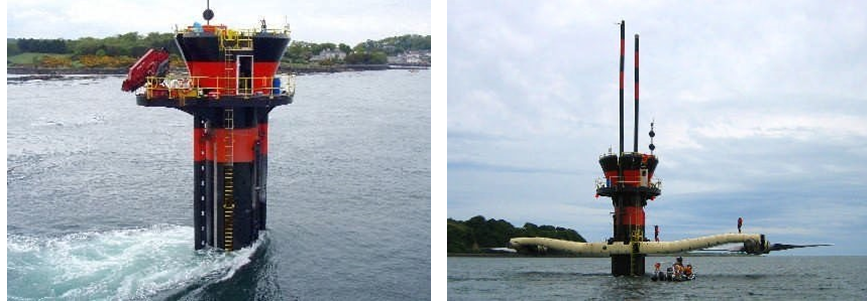
\includegraphics[width=12.04in]{figures/MCT} 

}

\caption{A current turbine}\label{fig:MCT}
\end{figure}

Typically, the impacts are assessed by means of surveys of animals, for example, observers counting the animals present at various times and recording their locations and estimating the animal populations. However, the distribution and number of animals might be effected by a number of other variables, such as tide-state, time of day, season etc., as well as the turbines.

If no impact was found, this might be due to the fact that not enough surveying was undertaken. So a typical question might be, `If animal numbers decreased by half after turbine construction, what amount of survey effort would be required to detect that change?' Alternatively, a range of scenarios might be considered, as in (Table \ref{tab:power}), where different population effects are considered as well as two different sampling regimes.

\label{tab:power} Power to detect an effect under different scenarios

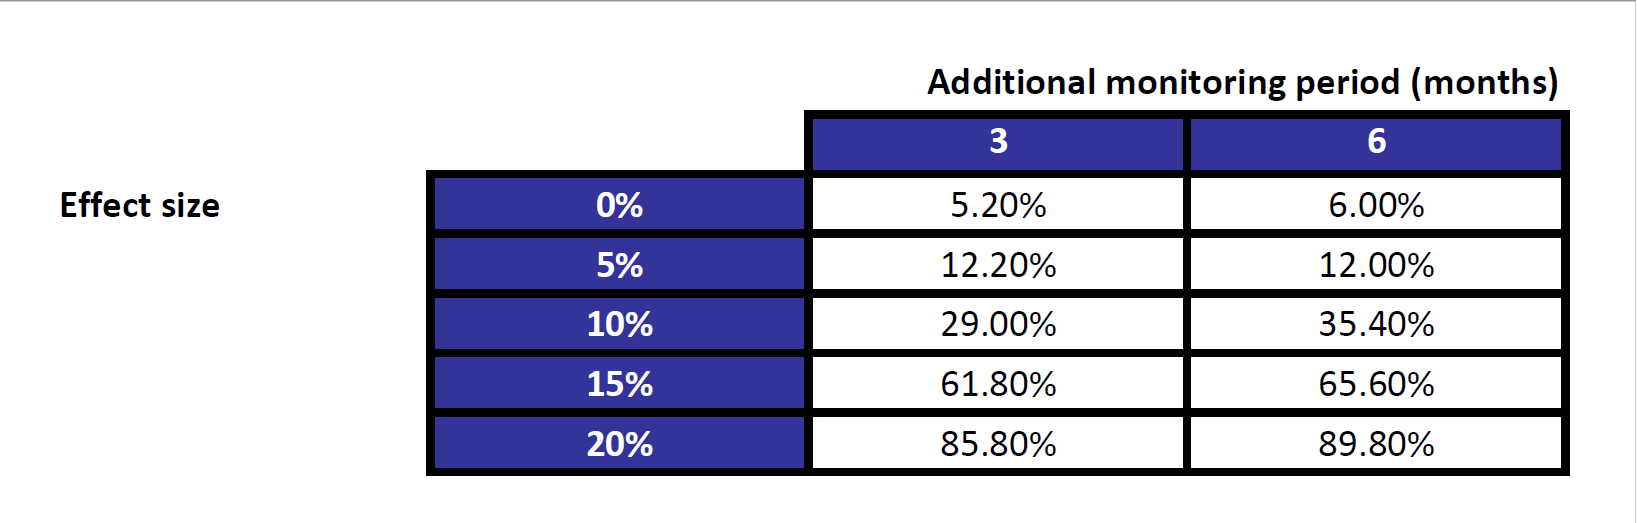
\includegraphics{figures/powerTableEIA.png}

\begin{itemize}
\tightlist
\item
  The power under various effect sizes and sampling regimes are given as percentages.
\item
  For example, expect almost 0.898 probability of detecting a 20\% reduction in the population if a further 6-months data are collected.
\end{itemize}

So power calculations are often required in order to determine how much data to collect. This will depend on:

\begin{itemize}
\tightlist
\item
  How big an effect do you need/hope to detect?
\item
  How much variability is in the system?
\item
  What level of power is needed?
\end{itemize}

Armed with this information, we can advise on sample size, \(n\), to meet these specifications. Knowing the variability is the crucial issue; estimates might be obtainable from previous studies, a new pilot study or as a last resort, a guess. An estimate of variance from a pilot study might be inaccurate if sample size was low.

\hypertarget{calculating-power}{%
\section{Calculating power}\label{calculating-power}}

(Example modified from Larsen \& Marx \citeyearpar{Larsen&Marx2006})

Imagine there is a new fuel additive that is expected to increase the fuel efficiency for vehicles. The underlying fuel efficiency with the standard fuel is assumed to be 25 mpg. It is thought an improvement of at least 3\% in fuel efficiency would be substantial enough for the additive to be taken to market. A trial is planned with the intention of detecting whether fuel efficiency with the additive has increased from 25 to 26 mpg (i.e.~an approximate 3\% increase) or even more.

We need to first identify our assumptions:

\begin{itemize}
\tightlist
\item
  Fuel efficiency in cars is normally distributed.
\item
  The standard deviation of efficiency in cars is claimed to be 2.4 (\(\sigma\)). We assume this is known (rather than estimated).
\end{itemize}

Assuming an effect size (improvement) to 26 mpg is desired, and a sample size of 30, what is the power and Type II error associated with this (one-sided) test scenario?

The underlying hypothesis test here is a one sample \(z\) test (because \(\sigma\) is known; if this were estimated, we would use a \(t\) test). The null and alternative hypotheses are:

\(H_0\): \(\hat \mu = 25\)
\(H_1\): \(\hat \mu > 25\)

The test is one tailed because we are considering an improvement in efficiency. It would be two-tailed is we were considering a difference in efficiency between the two fuels.

The test statistic is given by

\[ z_{stat} = \frac{\textrm{data-estimate} - \textrm{hypothesised value}}{\textrm{standard error(data-estimate)}} = \frac{\hat \mu - \textrm{hypothesised value}}{\frac{\sigma}{\sqrt{n}}}\]
We would reject \(H_0\) if \(z_{stat}\) is greater than the critical value, \(z_{crit}\), i.e.~\(z_{stat} > z_{crit}\):

\[ \frac{\hat \mu - \textrm{hypothesised value}}{\frac{\sigma}{\sqrt{n}}} > z_{crit}\]
Thus, we can rearrange this expression to provide a value of \(\hat \mu\) that would be required to reject \(H_0\):

\[\hat \mu > \textrm{hypothesised value} + \frac{\sigma}{\sqrt{n}}z_{crit}\]
Assuming the Type I error is 5\%, (\(\alpha\) = 0.05), we know that the one-tailed critical value, \(z_{crit}\), is:

\begin{Shaded}
\begin{Highlighting}[]
\FunctionTok{qnorm}\NormalTok{(}\AttributeTok{p=}\FloatTok{0.95}\NormalTok{)}
\end{Highlighting}
\end{Shaded}

\begin{verbatim}
[1] 1.644854
\end{verbatim}

The hypothesised value is 25, so that the critical value that would cause us to reject \(H_0\) can be calculated as follows:

\[25 + 1.644854 \times \frac{2.4}{\sqrt{30}} = 25.72\]

Figure \ref{fig:fuelplot} shows the probability density function under the null hypothesis i.e.~\(N(\mu=25, \sigma=2.4)\). The red shaded area indicates critical value that would lead us to rejecting the null hypothesis under \(\alpha = 0.05\).

\begin{figure}

{\centering \includegraphics{IntroStats_files/figure-latex/fuelplot-1} 

}

\caption{Probability density function of the reference distribution showing the Type I error region (red).}\label{fig:fuelplot}
\end{figure}

Hence, if our sample had a mean greater than 25.72 mpg we would reject \(H_0\). In rejecting the Null hypothesis we are at risk of making a Type I error. The Type II error, needs to be considered as well (Figure \ref{fig:fuelplot2}), relative to the alternative hypothesis. If \(H_1\) were true with its greater mean, and had the same standard deviation, we would produce false negatives (Type II) errors by falling left of this decision boundary.

\begin{figure}

{\centering \includegraphics{IntroStats_files/figure-latex/fuelplot2-1} 

}

\caption{Probability density function of reference distribution showing the Type I error region (red) and the Type II error region (purple).}\label{fig:fuelplot2}
\end{figure}

To calculate the purple false negative area if \(\mu = 26\) in R:

\begin{Shaded}
\begin{Highlighting}[]
\FunctionTok{pnorm}\NormalTok{(}\AttributeTok{q=}\FloatTok{25.72}\NormalTok{, }\AttributeTok{mean=}\DecValTok{26}\NormalTok{, }\AttributeTok{sd=}\FloatTok{2.4}\SpecialCharTok{/}\FunctionTok{sqrt}\NormalTok{(}\DecValTok{30}\NormalTok{), }\AttributeTok{lower.tail=}\ConstantTok{TRUE}\NormalTok{)}
\end{Highlighting}
\end{Shaded}

\begin{verbatim}
[1] 0.2614083
\end{verbatim}

\begin{itemize}
\tightlist
\item
  Thus, a Type II error occurs about 26.1\% of the time.
\item
  Power is \(1-\beta = 1 - 0.2614 = 0.7386\) i.e.~73.9\%
  Therefore, we would fail to find evidence of a 1 mpg improvement almost a quarter the time.
\end{itemize}

\hypertarget{increasing-the-power}{%
\subsection{Increasing the power}\label{increasing-the-power}}

In the above case the power might be thought of as not very high. The obvious adaptions to make an improvements to this poor power are:

\begin{itemize}
\tightlist
\item
  Increasing precision through larger samples.
\item
  Increasing precision through controlling variability (e.g.~testing on a standardised track or the like).
\item
  Accept a higher Type I error.
\item
  Have a fuel additive that is expected to have improvements much greater than 1 mpg.
\end{itemize}

\hypertarget{increasing-the-sample-size}{%
\subsubsection{Increasing the sample size}\label{increasing-the-sample-size}}

What happens if \(n\) is doubled?

\begin{itemize}
\tightlist
\item
  The decision boundary is now at:
\end{itemize}

\begin{Shaded}
\begin{Highlighting}[]
\NormalTok{decisionBound }\OtherTok{\textless{}{-}} \DecValTok{25}\FloatTok{+1.644854}\SpecialCharTok{*}\FloatTok{2.4}\SpecialCharTok{/}\FunctionTok{sqrt}\NormalTok{(}\DecValTok{60}\NormalTok{)}

\NormalTok{decisionBound}
\end{Highlighting}
\end{Shaded}

\begin{verbatim}
[1] 25.50964
\end{verbatim}

Therefore the false negative rate is

\begin{Shaded}
\begin{Highlighting}[]
\FunctionTok{pnorm}\NormalTok{(}\AttributeTok{q=}\NormalTok{decisionBound, }\AttributeTok{mean=}\DecValTok{26}\NormalTok{, }\AttributeTok{sd=}\FloatTok{2.4}\SpecialCharTok{/}\FunctionTok{sqrt}\NormalTok{(}\DecValTok{60}\NormalTok{))}
\end{Highlighting}
\end{Shaded}

\begin{verbatim}
[1] 0.05675267
\end{verbatim}

This means our Type II error is about 5.7\% - a power of 94.3\% (80\% is often the goal in planning).

\hypertarget{increasing-the-effect-size}{%
\subsubsection{Increasing the effect size}\label{increasing-the-effect-size}}

Bigger changes in effect size would give higher power too, for example, we could consider 26.5 mpg instead of 26 mpg:

\begin{Shaded}
\begin{Highlighting}[]
\FunctionTok{pnorm}\NormalTok{(}\AttributeTok{q=}\NormalTok{decisionBound, }\AttributeTok{mean=}\FloatTok{26.5}\NormalTok{, }\AttributeTok{sd=}\FloatTok{2.4}\SpecialCharTok{/}\FunctionTok{sqrt}\NormalTok{(}\DecValTok{60}\NormalTok{))}
\end{Highlighting}
\end{Shaded}

\begin{verbatim}
[1] 0.0006958301
\end{verbatim}

Power is now therefore 1 - 0.0007 = 99.9\%; increasing the signal-to-noise ratio improves power.

\hypertarget{accepting-a-higher-type-i-error-rate}{%
\subsubsection{Accepting a higher Type I error rate}\label{accepting-a-higher-type-i-error-rate}}

Accepting an increased Type I error (e.g.~\(\alpha=10\%\)) similarly improves power - it lowers the decision boundary in this problem, but this might be undesirable.

\begin{Shaded}
\begin{Highlighting}[]
\FunctionTok{qnorm}\NormalTok{(}\AttributeTok{p=}\FloatTok{0.9}\NormalTok{)}
\end{Highlighting}
\end{Shaded}

\begin{verbatim}
[1] 1.281552
\end{verbatim}

\begin{Shaded}
\begin{Highlighting}[]
\NormalTok{decisionBound }\OtherTok{\textless{}{-}} \DecValTok{25}\SpecialCharTok{+}\FunctionTok{qnorm}\NormalTok{(}\FloatTok{0.9}\NormalTok{)}\SpecialCharTok{*}\FloatTok{2.4}\SpecialCharTok{/}\FunctionTok{sqrt}\NormalTok{(}\DecValTok{30}\NormalTok{)}

\NormalTok{decisionBound}
\end{Highlighting}
\end{Shaded}

\begin{verbatim}
[1] 25.56155
\end{verbatim}

\begin{Shaded}
\begin{Highlighting}[]
\FunctionTok{pnorm}\NormalTok{(}\AttributeTok{q=}\NormalTok{decisionBound, }\AttributeTok{mean=}\DecValTok{26}\NormalTok{, }\AttributeTok{sd=}\FloatTok{2.4}\SpecialCharTok{/}\FunctionTok{sqrt}\NormalTok{(}\DecValTok{30}\NormalTok{))}
\end{Highlighting}
\end{Shaded}

\begin{verbatim}
[1] 0.1585039
\end{verbatim}

Therefore the new power is 1 - 15.9 = 84.1\%

\begin{itemize}
\tightlist
\item
  Given a Type II error of 26.1\% versus 15.9\% before (power moves from 73.9\% originally to 84.1\%).
\end{itemize}

Essentially, we are trading the probability of making one type of error for another.

\hypertarget{power-by-simulation}{%
\subsection{Power by simulation}\label{power-by-simulation}}

The above is a theoretical approach to the calculation of power; frequently these days, power is estimated by simulation. This is often a more intuitive approach.

Using the above case, we assume the true mean was normally distributed with mean 26 mpg and standard deviation 2.4. If 1000 samples (of size 30) are randomly generated from this distribution and the sample mean calculated each time, the proportion of the means greater than the critical value from the Null distribution (i.e.~assuming \(\mu\) =25) would give the power. The code below implements this process.

\begin{Shaded}
\begin{Highlighting}[]
\CommentTok{\# Initialise vector to store results}
\NormalTok{value }\OtherTok{\textless{}{-}} \ConstantTok{NA}
\FunctionTok{set.seed}\NormalTok{ (}\DecValTok{101}\NormalTok{)}
\CommentTok{\# Critical value}
\NormalTok{zcrit }\OtherTok{\textless{}{-}} \FunctionTok{qnorm}\NormalTok{ (}\AttributeTok{p=}\FloatTok{0.95}\NormalTok{, }\AttributeTok{mean=}\DecValTok{25}\NormalTok{, }\AttributeTok{sd=}\FloatTok{2.4}\SpecialCharTok{/}\FunctionTok{sqrt}\NormalTok{(}\DecValTok{30}\NormalTok{))}

\CommentTok{\# Begin loop}
\ControlFlowTok{for}\NormalTok{ (i }\ControlFlowTok{in} \DecValTok{1}\SpecialCharTok{:}\DecValTok{1000}\NormalTok{) \{}
  \CommentTok{\# Generate random sample}
\NormalTok{  samplepower }\OtherTok{\textless{}{-}} \FunctionTok{rnorm}\NormalTok{ (}\AttributeTok{n=}\DecValTok{30}\NormalTok{, }\AttributeTok{mean=}\DecValTok{26}\NormalTok{, }\AttributeTok{sd=}\FloatTok{2.4}\NormalTok{) }\DocumentationTok{\#\#\#this is truth}
  \CommentTok{\# Test mean of sample, if \textgreater{} zcrit value=1, otherwise value=0}
  \ControlFlowTok{if}\NormalTok{ (}\FunctionTok{mean}\NormalTok{(samplepower) }\SpecialCharTok{\textgreater{}}\NormalTok{ zcrit) \{value[i]}\OtherTok{=}\DecValTok{1}\NormalTok{\}}
  \ControlFlowTok{else}\NormalTok{ \{(value[i]}\OtherTok{=}\DecValTok{0}\NormalTok{)\}}
\NormalTok{\} }\CommentTok{\# End loop}

\CommentTok{\# Calculate proportion}
\NormalTok{power }\OtherTok{\textless{}{-}} \FunctionTok{sum}\NormalTok{(value)}\SpecialCharTok{/}\DecValTok{1000}
\NormalTok{power}
\end{Highlighting}
\end{Shaded}

\begin{verbatim}
[1] 0.757
\end{verbatim}

The generated power is similar to 73.8\%, the value obtained above using a theoretical approach. If the number of iterations is increased the generated power converges ever closer to 73.8\%.

Similarly, if the sample size is increased to 60 (i.e.~n = 60 above) then an answer similar to the theoretical figure of approximately 94.3\% is obtained.

\begin{Shaded}
\begin{Highlighting}[]
\CommentTok{\# Initialise vector to store results}
\NormalTok{value }\OtherTok{\textless{}{-}} \ConstantTok{NA}
\FunctionTok{set.seed}\NormalTok{ (}\DecValTok{101}\NormalTok{)}
\CommentTok{\# Critical value}
\NormalTok{zcrit }\OtherTok{\textless{}{-}} \FunctionTok{qnorm}\NormalTok{ (}\AttributeTok{p=}\FloatTok{0.95}\NormalTok{, }\AttributeTok{mean=}\DecValTok{25}\NormalTok{, }\AttributeTok{sd=}\FloatTok{2.4}\SpecialCharTok{/}\FunctionTok{sqrt}\NormalTok{(}\DecValTok{60}\NormalTok{))}

\CommentTok{\# Begin loop}
\ControlFlowTok{for}\NormalTok{ (i }\ControlFlowTok{in} \DecValTok{1}\SpecialCharTok{:}\DecValTok{1000}\NormalTok{) \{}
  \CommentTok{\# Generate random sample}
\NormalTok{  samplepower }\OtherTok{\textless{}{-}} \FunctionTok{rnorm}\NormalTok{ (}\AttributeTok{n=}\DecValTok{60}\NormalTok{, }\AttributeTok{mean=}\DecValTok{26}\NormalTok{, }\AttributeTok{sd=}\FloatTok{2.4}\NormalTok{) }\DocumentationTok{\#\#\#this is truth}
  \CommentTok{\# Test mean of sample, if \textgreater{} zcrit value=1, otherwise value=0}
  \ControlFlowTok{if}\NormalTok{ (}\FunctionTok{mean}\NormalTok{(samplepower) }\SpecialCharTok{\textgreater{}}\NormalTok{ zcrit) \{value[i]}\OtherTok{=}\DecValTok{1}\NormalTok{\}}
  \ControlFlowTok{else}\NormalTok{ \{(value[i]}\OtherTok{=}\DecValTok{0}\NormalTok{)\}}
\NormalTok{\} }\CommentTok{\# End loop}

\CommentTok{\# Calculate proportion}
\NormalTok{power }\OtherTok{\textless{}{-}} \FunctionTok{sum}\NormalTok{(value)}\SpecialCharTok{/}\DecValTok{1000}
\NormalTok{power}
\end{Highlighting}
\end{Shaded}

\begin{verbatim}
[1] 0.95
\end{verbatim}

An interactive example of simulation based power analysis with varying sample size is in Figure \ref{fig:powshiny}. There is also a live version \href{https://moniquemackenzie.shinyapps.io/IntroStats_PowerDemo/}{here}



\begin{figure}

{\centering \href{https://moniquemackenzie.shinyapps.io/IntroStats_PowerDemo/}{\includegraphics{IntroStats_files/figure-latex/powshiny-1} }

}

\caption{An example of simulation based power analysis. You can see a live version by clicking \href{https://moniquemackenzie.shinyapps.io/IntroStats_PowerDemo/}{here}}\label{fig:powshiny}
\end{figure}

\hypertarget{multiple-comparisons-1}{%
\subsection{Multiple comparisons}\label{multiple-comparisons-1}}

When we make multiple comparisons and we adjust the family wise error rate (see the previous chapter) we are decreasing the risk of a Type I error but increasing the risk of a Type II error leading to a lower power.

\begin{itemize}
\tightlist
\item
  We make our Type I error boundaries more stringent (broader) i.e.~lower threshold \(p\)-values.
\item
  We are trading errors at some level, i.e., if the Type II errors increase, the power decreases.
\end{itemize}

\hypertarget{SUMpower}{%
\section{Summary}\label{SUMpower}}

Power should be an essential component of planning a statistical investigation. As mentioned above, a common convention is that a study should have a priori power of c.~80\% to be viable. Small sample sizes, trying to distinguish very small effect sizes and sloppy measurement with high variance will decrease the power of a test and lead to a low probability of rejecting \(H_0\). If these activities are undertaken to deliberately fail to reject \(H_0\) then this would be scientific misconduct.

There are myths propagated in some scientific disciplines about statistical power, namely that the power of a test can be assessed post-hoc to determine if the found negative results are justified. To be blunt, this is \emph{nonsense}. Power is numerically related to probability for a given Null hypothesis, therefore, any result which fails to reject the null hypothesis will have low power. It is meaningless to calculate power post-hoc as a way of ascertaining the appropriateness of a null result.

\hypertarget{learning-objectives-2}{%
\subsection{Learning Objectives}\label{learning-objectives-2}}

At the end of this chapter you should:

\begin{enumerate}
\def\labelenumi{\arabic{enumi}.}
\tightlist
\item
  understand power and its appropriate uses.
\item
  calculate simple power statistics
\item
  understand when power should not be used.
\end{enumerate}

\hypertarget{ANSpower}{%
\section{Answers}\label{ANSpower}}

\textbf{Q9.1} Power is all about the signal to noise ratio. So one can either

\begin{itemize}
\tightlist
\item
  increase the signal i.e.~assume a bigger effect size or
\item
  decrease the noise i.e.~increase the precision typically by increasing sample size.
\end{itemize}

\hypertarget{proportions}{%
\chapter{Proportions}\label{proportions}}

\emph{There is no excellent beauty that hath not some strangeness in the proportion.}
Sir Francis Bacon \citeyearpar{Bacon1696}

\hypertarget{INTprop}{%
\section{Introduction}\label{INTprop}}

Data often come as counts or frequencies which can be transformed to proportions. For example, imagine a survey where at each of several locations, the presence or absence of one or more birds is noted. The proportion of locations where a bird was located can be obtained from

\[\textrm{proportion of bird locations} = \frac{\textrm{number of locations where one or more birds are seen}}{\textrm{total number of locations}}\]

We can use the observed proportion to estimate the probability of seeing one or more birds at a particular locality, \(x\), out of the number of trials, \(n\), to estimate the probability of success, \(p\):

\[\hat p = \frac{x}{n}\]

Hence, we estimate the true underlying probability \(p\) with the sample proportion \(\hat p\). If different locations had been sampled, then the observed proportion of locations where a bird was detected would likely change. There is some uncertainty associated with the sample proportions. Therefore in this chapter we consider:

\begin{itemize}
\tightlist
\item
  confidence intervals for proportions
\item
  confidence intervals for a difference in proportions and
\item
  a hypothesis test for a proportion.
\end{itemize}

Proportions and probabilities are similar in that they are both bounded by 0 and 1 and the terms are often used interchangeably, not least because the sample proportion is frequently used to estimate the underlying (but unknown) population probability of success.

In some cases, looking at the difference between proportions is not possible or relevant and so a ratio is obtained - this is called an odds ratio and discussed at the end of this chapter.

\hypertarget{confidence-intervals}{%
\section{Confidence intervals}\label{confidence-intervals}}

To illustrate the formulation of CI for a proportion, we can consider the bird survey mentioned above. Imagine the birds were surveyed at three different time periods (perhaps before (which we will call phase A), during (phase B) and after (phase C) the building of a windfarm. There are two obvious questions of interest: in what proportion of localities will a bird be seen and what is the difference in the proportion of birds seen between the phases?

To estimate the proportion of localities with birds in this region assume that the number of locations where a bird was detected \(x\) is a random variable from a binomial distribution with known \(n\) (fixed number of trials, i.e.~all sampling locations) and unknown \(p\) (probability of success).

We will estimate the proportion of `successful' observations, \(p\), from the number of observations with sightings (`successes') and the total number of observations (`trials').

Recall, there are 4 conditions of the binomial distribution:

\begin{enumerate}
\def\labelenumi{\arabic{enumi}.}
\tightlist
\item
  two outcomes for each trial,
\item
  the same probability of success for each trial,
\item
  a fixed number of trials,
\item
  independence of trials.
\end{enumerate}

\textbf{Q11.1} How realistic are these conditions for the wind farm data?

\hypertarget{exploratory-data-analysis}{%
\subsection{Exploratory data analysis}\label{exploratory-data-analysis}}

Trained observers recorded the presence or absence of birds at each spatial location:

\begin{itemize}
\tightlist
\item
  when birds were seen in some defined location a presence (success) was recorded
\item
  and when birds were not seen it was recorded as an absence (failure).
\end{itemize}

We estimate the probability of sighting an animal using:

\[\hat{p}=\frac{\text{number of successes}}{\text{number of trials}} \]

which in the wind farm data, as mentioned in the introduction, translates to:

\[\hat p = \frac{\textrm{number of observations where one or more birds were seen}}{\textrm{total number of observations}}\]
For each phase we have the number of successful observations and the number of observations in total (Table \ref{tab:phasetab}). \\

\label{tab:phasetab} Number of presence (1) or absence (0) observations in phases A, B and C in the building of a windfarm.

\begin{longtable}[]{@{}cccc@{}}
\toprule
\begin{minipage}[b]{(\columnwidth - 3\tabcolsep) * \real{0.17}}\centering
~\strut
\end{minipage} & \begin{minipage}[b]{(\columnwidth - 3\tabcolsep) * \real{0.11}}\centering
A\strut
\end{minipage} & \begin{minipage}[b]{(\columnwidth - 3\tabcolsep) * \real{0.11}}\centering
B\strut
\end{minipage} & \begin{minipage}[b]{(\columnwidth - 3\tabcolsep) * \real{0.11}}\centering
C\strut
\end{minipage}\tabularnewline
\midrule
\endhead
\begin{minipage}[t]{(\columnwidth - 3\tabcolsep) * \real{0.17}}\centering
\textbf{0}\strut
\end{minipage} & \begin{minipage}[t]{(\columnwidth - 3\tabcolsep) * \real{0.11}}\centering
10335\strut
\end{minipage} & \begin{minipage}[t]{(\columnwidth - 3\tabcolsep) * \real{0.11}}\centering
12495\strut
\end{minipage} & \begin{minipage}[t]{(\columnwidth - 3\tabcolsep) * \real{0.11}}\centering
5436\strut
\end{minipage}\tabularnewline
\begin{minipage}[t]{(\columnwidth - 3\tabcolsep) * \real{0.17}}\centering
\textbf{1}\strut
\end{minipage} & \begin{minipage}[t]{(\columnwidth - 3\tabcolsep) * \real{0.11}}\centering
1143\strut
\end{minipage} & \begin{minipage}[t]{(\columnwidth - 3\tabcolsep) * \real{0.11}}\centering
1633\strut
\end{minipage} & \begin{minipage}[t]{(\columnwidth - 3\tabcolsep) * \real{0.11}}\centering
460\strut
\end{minipage}\tabularnewline
\begin{minipage}[t]{(\columnwidth - 3\tabcolsep) * \real{0.17}}\centering
\textbf{Total}\strut
\end{minipage} & \begin{minipage}[t]{(\columnwidth - 3\tabcolsep) * \real{0.11}}\centering
11478\strut
\end{minipage} & \begin{minipage}[t]{(\columnwidth - 3\tabcolsep) * \real{0.11}}\centering
14128\strut
\end{minipage} & \begin{minipage}[t]{(\columnwidth - 3\tabcolsep) * \real{0.11}}\centering
5896\strut
\end{minipage}\tabularnewline
\bottomrule
\end{longtable}

From this summary information we estimate the sighting probabilities in each phase as follows:

\[\hat p_{A} = \frac{1143}{11478} = 0.0996 \quad; \quad \hat p_{B} = \frac{1633}{14128} = 0.1156 \quad ; \quad \hat p_{C} = \frac{460}{5896} = 0.0780\]
We can estimate similar probabilities for each year and month (Figure \ref{fig:barplotfig2}) of the survey. The before period was from 2000 to 2002 inclusive, the during period was 2003 and 2007 and the after period was 2011.

\begin{figure}

{\centering \includegraphics{IntroStats_files/figure-latex/barplotfig2-1} 

}

\caption{Barplot showing the mean sightings probability for every year/month combination. N.B.Not all months are labelled}\label{fig:barplotfig2}
\end{figure}

From this information (Figure \ref{fig:barplotfig2}) we see that:

\begin{itemize}
\tightlist
\item
  the proportion of sighting a bird appears to be higher in phase B compared with the phases A and C,
\item
  and the proportion of sighting a bird tends to be highest in January-March of each year.
\end{itemize}

While some patterns are apparent, it is difficult to tell if the observed differences are genuine differences across phases and/or year-month combinations or if these differences are due to sampling error; would these differences have been seen even if the true underlying (but unknown) probability of sighting for all phases (and/or year-month combinations) was the same? To assess the uncertainty associated with a sample proportion, we build a confidence interval and the formulation of the interval depends on the number of trials, \(n\), and on the value of \(p\).

\hypertarget{confidence-intervals-large-sample-sizes}{%
\subsection{Confidence intervals: large sample sizes}\label{confidence-intervals-large-sample-sizes}}

While the number of successes from the number of trials is assumed to be a binomial random variable, the sample proportions (estimates for \(p\); \(\hat{p}\)) are normally distributed about the true (underlying) population proportion if the number of trials is \textbf{large}. Therefore, confidence intervals (CIs) for proportions are constructed in a similar way to CIs for large samples of normal data. For large samples, the sample porportion is approximately normally distributed:

\[\hat{p} \sim normal \left(p, se({p})\right)\]
However, since we never know \(p\), we use the sample proportion \(\hat p\), thus, the standard deviation of the sample proportion (the standard error) can be found using:

\[se(\hat{p})=\sqrt{\frac{\hat p (1-\hat p)}{n}}\]
Just as with means we can create 95\% confidence interval on the proportions.

To find a \textbf{95\% confidence interval} for \(p\) we use a familiar structure:
\begin{align*}
          \textrm{estimate}~~ &\pm z_{1-\frac{\alpha}{2}} \times~~ \textrm{standard error}\\
          \hat{p} & \pm 1.96 \times \sqrt{\frac{\hat{p} (1-\hat{p})}{n}}
\end{align*}

where \(\alpha=0.05\) for a 95\% CI, hence \(z_{0.025}\).

\hypertarget{how-large-is-large-enough}{%
\subsubsection{How large is large enough?}\label{how-large-is-large-enough}}

To assume these estimates are approximately normally distributed about \(p\) we require large samples. As the number of trials increases, the distribution becomes more and more like the normal distribution until the sample size is so large that the distribution is exactly normally distributed - it has reached a limit, or asymptote, hence, these CI are sometimes called `asymptotic' confidence intervals. However, the required sample size changes with \(\hat{p}\).

The minimum sample sizes for different values of \(\hat p\) are given in Table \ref{tab:samplesizeprop}. Thus if p is very small 0.05 or large 0.95, a sample size of at least 960 would be required in order to assume that the proportion is normally distributed.:

\label{tab:samplesizeprop} Sample sizes for to assume large-sample properties for proportions

\begin{table}
\label{samplesizeprop}
\caption{Sample sizes for to assume large-sample properties for proportions}
\end{table}

\begin{longtable}[]{@{}ccccccccccc@{}}
\toprule
Value for \(\hat{p}\) & 0.05 & 0.1 & 0.15 & 0.2 & 0.25 & 0.3 & 0.35 & 0.4 & 0.45 & 0.5\tabularnewline
\midrule
\endhead
Minimum \(n\) & 960 & 400 & 220 & 125 & 76 & 47 & 23 & 13 & 11 & 10\tabularnewline
Value for \(\hat{p}\) & 0.95 & 0.9 & 0.85 & 0.8 & 0.75 & 0.7 & 0.65 & 0.6 & 0.55 & 0.5\tabularnewline
\bottomrule
\end{longtable}

\textbf{Example} We are going to build 95\% CIs for the proportion of sighting birds in phases A, B and C. The total number of sampled locations (\(n\)) for each phase is greater than 1000 and so results based on these large-sample properties should be valid.

The CI for Phase A is constructed as follows: we estimated \(p_A\) previously, \(\hat p_A = 0.0996\) and the standard error is given by:

\[se(\hat{p_A})=\sqrt{\frac{\hat{p_A}(1-\hat{p_A})}{n}}=
          \sqrt{\frac{0.0996(1-0.0996)}{11478}}=  0.0028\]

\begin{align*}
95\%~ \textrm{CI}=&\hat{p} \pm z_{0.025} \times se(\hat{p})\\
=&0.0996 \pm 1.96 \times 0.0028\\
=& (0.0941,0.1051)
\end{align*}

Based on these results we can be 95\% confident that the proportion of locations with a bird in Phase \emph{A} is somewhere between 0.094 (9.4\%) and 0.105 (10.5\%).

We find 95\% CI for the proportions in phases B and C and thus can say,

\begin{itemize}
\item
  with 95\% confidence we estimate the proportion of a location with a bird in this region in Phase B to be somewhere between 0.11, 0.121
\item
  with 95\% confidence we estimate the proportion of a location with a bird in this region in Phase C to be somewhere between 0.071, 0.085.
\end{itemize}

\hypertarget{doing-this-in-r-19}{%
\subsubsection{Doing this in R}\label{doing-this-in-r-19}}

To calculate these confidence intervals in R, an additional package is required \texttt{Hmisc} \citep{R-Hmisc}:

\begin{Shaded}
\begin{Highlighting}[]
\CommentTok{\# Load package}
\FunctionTok{library}\NormalTok{(Hmisc)}
\CommentTok{\# 95\% CI using asymptotic normal approximation; x=number of successes; }
\CommentTok{\#   n=number of trials}
\FunctionTok{binconf}\NormalTok{(}\AttributeTok{x=}\DecValTok{1143}\NormalTok{, }\AttributeTok{n=}\DecValTok{11478}\NormalTok{, }\AttributeTok{alpha=}\FloatTok{0.05}\NormalTok{, }\AttributeTok{method=}\StringTok{"asymptotic"}\NormalTok{)}
\end{Highlighting}
\end{Shaded}

\begin{verbatim}
   PointEst      Lower     Upper
 0.09958181 0.09410374 0.1050599
\end{verbatim}

\hypertarget{confidence-intervals-small-sample-sizes}{%
\subsection{Confidence intervals: small sample sizes}\label{confidence-intervals-small-sample-sizes}}

For `small' samples (less than those in the table above) when \(p\) is close to zero or one, assuming the proportions are normally distributed is not valid.

To illustrate this we calculate the 95\% CI for \(\hat p=0.1\) and \(n=10\).

\[se(\hat p) = \sqrt{\frac{0.1 (1-0.1)}{10}} = 0.0949\]

Hence, the CI is given by

\[0.1 \pm 1.96*0.0949\]
\[0.1 \pm 0.1859 \]
\[-0.086 \quad ; \quad 0.286 \]

The lower limit is less than 0 and a proportion cannot be negative. Therefore, a different formulation is required for small sample sizes.

The literature suggests that \textbf{Wilson intervals} are preferred in these cases \citep{Agresti1998}. This has a rather more complicated formula:

\[\frac{1}{1+{\frac{1}{n}}z^{2}}\left[{\hat {p}}+{\frac{1}{2n}}z^{2}\pm z{\sqrt{{\frac {1}{n}}{\hat{p}}\left(1-{\hat{p}}\right)+{\frac {1}{4n^{2}}}z^{2}}}\right]\]
(and so we will be using \texttt{R} to calculate these values.)

This approach ensures that the confidence interval limits never extend below zero or above one.

For example, Table \ref{tab:compwilson} the asymptotic (i.e.~using the normal distribution) and Wilson confidence intervals are calculated when we have one success and 10 trials (i.e.~\(p=0.1\)):

\label{tab:compwilson} Comparison of Wilson and asymptotic confidence intervals

\begin{longtable}[]{@{}cccc@{}}
\toprule
\begin{minipage}[b]{(\columnwidth - 3\tabcolsep) * \real{0.24}}\centering
~\strut
\end{minipage} & \begin{minipage}[b]{(\columnwidth - 3\tabcolsep) * \real{0.15}}\centering
PointEst\strut
\end{minipage} & \begin{minipage}[b]{(\columnwidth - 3\tabcolsep) * \real{0.15}}\centering
Lower\strut
\end{minipage} & \begin{minipage}[b]{(\columnwidth - 3\tabcolsep) * \real{0.15}}\centering
Upper\strut
\end{minipage}\tabularnewline
\midrule
\endhead
\begin{minipage}[t]{(\columnwidth - 3\tabcolsep) * \real{0.24}}\centering
\textbf{Wilson}\strut
\end{minipage} & \begin{minipage}[t]{(\columnwidth - 3\tabcolsep) * \real{0.15}}\centering
0.1\strut
\end{minipage} & \begin{minipage}[t]{(\columnwidth - 3\tabcolsep) * \real{0.15}}\centering
0.005129\strut
\end{minipage} & \begin{minipage}[t]{(\columnwidth - 3\tabcolsep) * \real{0.15}}\centering
0.4042\strut
\end{minipage}\tabularnewline
\begin{minipage}[t]{(\columnwidth - 3\tabcolsep) * \real{0.24}}\centering
\textbf{Asymptotic}\strut
\end{minipage} & \begin{minipage}[t]{(\columnwidth - 3\tabcolsep) * \real{0.15}}\centering
0.1\strut
\end{minipage} & \begin{minipage}[t]{(\columnwidth - 3\tabcolsep) * \real{0.15}}\centering
-0.08594\strut
\end{minipage} & \begin{minipage}[t]{(\columnwidth - 3\tabcolsep) * \real{0.15}}\centering
0.2859\strut
\end{minipage}\tabularnewline
\bottomrule
\end{longtable}

The lower limit for the confidence interval based on the normal distribution is negative - an inplausible value for a proportion.

According to our table of `what is large', when \(\hat{p} = 0.1\), we should have a sample size of more than 400 to use the method based on the normal distribution.

If we increase the number of trials to 1000, (and the number of success to 100 so that \(\hat{p}=0.1\)), then the asymptotic normal distribution-based interval no longer gives impossible values.

\begin{longtable}[]{@{}cccc@{}}
\toprule
\begin{minipage}[b]{(\columnwidth - 3\tabcolsep) * \real{0.24}}\centering
~\strut
\end{minipage} & \begin{minipage}[b]{(\columnwidth - 3\tabcolsep) * \real{0.15}}\centering
PointEst\strut
\end{minipage} & \begin{minipage}[b]{(\columnwidth - 3\tabcolsep) * \real{0.14}}\centering
Lower\strut
\end{minipage} & \begin{minipage}[b]{(\columnwidth - 3\tabcolsep) * \real{0.14}}\centering
Upper\strut
\end{minipage}\tabularnewline
\midrule
\endhead
\begin{minipage}[t]{(\columnwidth - 3\tabcolsep) * \real{0.24}}\centering
\textbf{Wilson}\strut
\end{minipage} & \begin{minipage}[t]{(\columnwidth - 3\tabcolsep) * \real{0.15}}\centering
0.1\strut
\end{minipage} & \begin{minipage}[t]{(\columnwidth - 3\tabcolsep) * \real{0.14}}\centering
0.08291\strut
\end{minipage} & \begin{minipage}[t]{(\columnwidth - 3\tabcolsep) * \real{0.14}}\centering
0.1202\strut
\end{minipage}\tabularnewline
\begin{minipage}[t]{(\columnwidth - 3\tabcolsep) * \real{0.24}}\centering
\textbf{Asymptotic}\strut
\end{minipage} & \begin{minipage}[t]{(\columnwidth - 3\tabcolsep) * \real{0.15}}\centering
0.1\strut
\end{minipage} & \begin{minipage}[t]{(\columnwidth - 3\tabcolsep) * \real{0.14}}\centering
0.08141\strut
\end{minipage} & \begin{minipage}[t]{(\columnwidth - 3\tabcolsep) * \real{0.14}}\centering
0.1186\strut
\end{minipage}\tabularnewline
\bottomrule
\end{longtable}

However, note that for very small estimates of \(p\), Wilson intervals are still preferred even if the number of trials is large.

For our wind farm data, the Wilson intervals for the proportions of locations are givein in Table \ref{tab:compphases}:

\label{tab:compphases} Comparison of Wilson confidence intervals for the windfarm phases

\begin{longtable}[]{@{}cccc@{}}
\toprule
\begin{minipage}[b]{(\columnwidth - 3\tabcolsep) * \real{0.11}}\centering
Phase\strut
\end{minipage} & \begin{minipage}[b]{(\columnwidth - 3\tabcolsep) * \real{0.15}}\centering
PointEst\strut
\end{minipage} & \begin{minipage}[b]{(\columnwidth - 3\tabcolsep) * \real{0.14}}\centering
Lower\strut
\end{minipage} & \begin{minipage}[b]{(\columnwidth - 3\tabcolsep) * \real{0.14}}\centering
Upper\strut
\end{minipage}\tabularnewline
\midrule
\endhead
\begin{minipage}[t]{(\columnwidth - 3\tabcolsep) * \real{0.11}}\centering
A\strut
\end{minipage} & \begin{minipage}[t]{(\columnwidth - 3\tabcolsep) * \real{0.15}}\centering
0.09958\strut
\end{minipage} & \begin{minipage}[t]{(\columnwidth - 3\tabcolsep) * \real{0.14}}\centering
0.09424\strut
\end{minipage} & \begin{minipage}[t]{(\columnwidth - 3\tabcolsep) * \real{0.14}}\centering
0.1052\strut
\end{minipage}\tabularnewline
\begin{minipage}[t]{(\columnwidth - 3\tabcolsep) * \real{0.11}}\centering
B\strut
\end{minipage} & \begin{minipage}[t]{(\columnwidth - 3\tabcolsep) * \real{0.15}}\centering
0.1156\strut
\end{minipage} & \begin{minipage}[t]{(\columnwidth - 3\tabcolsep) * \real{0.14}}\centering
0.1104\strut
\end{minipage} & \begin{minipage}[t]{(\columnwidth - 3\tabcolsep) * \real{0.14}}\centering
0.121\strut
\end{minipage}\tabularnewline
\begin{minipage}[t]{(\columnwidth - 3\tabcolsep) * \real{0.11}}\centering
C\strut
\end{minipage} & \begin{minipage}[t]{(\columnwidth - 3\tabcolsep) * \real{0.15}}\centering
0.07802\strut
\end{minipage} & \begin{minipage}[t]{(\columnwidth - 3\tabcolsep) * \real{0.14}}\centering
0.07144\strut
\end{minipage} & \begin{minipage}[t]{(\columnwidth - 3\tabcolsep) * \real{0.14}}\centering
0.08514\strut
\end{minipage}\tabularnewline
\bottomrule
\end{longtable}

These are very similar to the CI we calculated earlier; this is not surprising since the numbers of trials are so large.

\begin{figure}

{\centering \includegraphics{IntroStats_files/figure-latex/barplotcifig-1} 

}

\caption{Barplot showing the mean sightings probability for each of the three phases. The black lines are 95\% Wilsons confidence intervals.}\label{fig:barplotcifig}
\end{figure}

\hypertarget{doing-this-in-r-20}{%
\subsubsection{Doing this in R}\label{doing-this-in-r-20}}

Wilson confidence intervals are obtained by specifying \texttt{method="wilson}.

\begin{Shaded}
\begin{Highlighting}[]
\CommentTok{\# Wilson\textquotesingle{}s CI for p=0.1 and number of trials is 10}
\FunctionTok{binconf}\NormalTok{(}\AttributeTok{x=}\DecValTok{1}\NormalTok{, }\AttributeTok{n=}\DecValTok{10}\NormalTok{, }\AttributeTok{alpha=}\FloatTok{0.05}\NormalTok{, }\AttributeTok{method=}\StringTok{"wilson"}\NormalTok{)}
\end{Highlighting}
\end{Shaded}

\begin{verbatim}
 PointEst       Lower   Upper
      0.1 0.005129329 0.40415
\end{verbatim}

\hypertarget{comparing-two-proportions-the-z-test}{%
\section{\texorpdfstring{Comparing two proportions: the \(z\) test}{Comparing two proportions: the z test}}\label{comparing-two-proportions-the-z-test}}

In this section we compare two proportions and again use the wind farm data as a motivating example.

While there appears to be some differences across phases based on the results obtained so far, in order to statistically answer questions about changes in proportions over time, we need to formally test for differences between the groups (e.g.~between phases or between different years or months).

Rather than use confidence intervals, which give a range of likely values for each parameter, we test for \textbf{no difference} between the two parameter values and evaluate the strength of evidence against this null hypothesis. We \textbf{formally} compare two proportions with a hypothesis test, which uses the normal distribution as the reference distribution (known as a \(z\) test).

So for example, we examine if there have been changes between phases in the wndfarm data by comparing the differences we have observed between phases with the sorts of differences we would expect to see even if no genuine changes have occurred.

\hypertarget{testing-for-no-difference-between-groups}{%
\subsection{Testing for `no difference' between groups}\label{testing-for-no-difference-between-groups}}

In order to test the research hypothesis that sighting proportions were different in phase A (\(p_{A}\)) and phase C (\(p_{C}\)) we take the following steps:

\begin{itemize}
\tightlist
\item
  We test this research hypothesis using the (skeptical) null hypothesis of no difference (\(H_0\)) and a `two-sided' alternative hypothesis (\(H_1\)) of either a positive or negative difference:
\end{itemize}

\[H_0: p_{A}-p_{C}=0\]

\[H_1: p_{A}-p_{C} \neq 0\]

\begin{itemize}
\item
  We evaluate the null hypothesis by considering what we would expect to see if the null hypothesis is true. For example,

  \begin{itemize}
  \tightlist
  \item
    if there has been no difference in sighting probabilities between phases then we would expect to see small differences in the sighting rates across phases.
  \item
    small differences like these (based on sampling variability alone) provide us with the background for comparison with the differences we did observe across phases.
  \end{itemize}
\item
  We compare our data-estimate (i.e.~the difference between \(p_{A}\) and \(p_{C}\)) with the hypothesised value (for no difference, or zero, in this case):
\end{itemize}

\[\textrm{data-estimate} - \textrm{hypothesised value}\]

\begin{itemize}
\tightlist
\item
  Our data-estimate for the difference between the proportions is:
\end{itemize}

\begin{center}
$$\hat{p}_{A}-\hat{p}_{C}= 0.0996 - 0.078 = 0.0216 $$
\end{center}

\begin{itemize}
\item
  the hypothesised value is 0, therefore our estimate is 0.0216 units.
\item
  While the point estimate (of 0.0216) is useful, we know that if we had taken data from slightly different locations or at slightly different times we would have obtained a different set of data and so we need to consider the uncertainty in our estimate.
\item
  The uncertainty in the estimate of the difference between the proportions can be quantified by the \textbf{standard error of the difference}:
\end{itemize}

\begin{align*}
se(\hat{p}_A-\hat{p}_C)=&\sqrt{\frac{\hat{p}_A(1-\hat{p}_A)}{n_A}+\frac{\hat{p}_C(1-\hat{p}_C)}{n_C}}\\
\end{align*}

\begin{align*}
=& \sqrt{\frac{0.0996(1-0.0996)}{11478}+\frac{0.078(1-0.078)}{5896}}\\
= &   0.004\\
\end{align*}

This method of calculating the uncertainty in our estimate (the standard error formula) requires these sample proportions are independent.

Do you think this is realistic in this case?

\hypertarget{how-does-our-estimate-compare-with-the-differences-we-might-expect}{%
\subsubsection{How does our estimate compare with the differences we might expect?}\label{how-does-our-estimate-compare-with-the-differences-we-might-expect}}

Once we have quantified the uncertainty about our estimate we can represent the difference seen between sample proportions as a ratio of the standard error.

\[\text{test statistic} = \frac{\text{difference - hypothesised value}}{\text{standard error}}\]

This puts our estimate for the difference into perspective:

\begin{itemize}
\item
  small differences can look large if the standard error is small (and our estimate has high precision/low uncertainty) and
\item
  large differences can look small (if our estimate has low precision/high uncertainty).
\end{itemize}

In our example, even an apparently small difference is actually large when we consider the high precision/low uncertainty about the estimate:

\begin{align*}
\textrm{test statistic} =&\frac{\textrm{difference-hypothesised value}}{\textrm{standard error}}\\
=& \frac{0.022}{0.004} = 
4.82\\
\end{align*}

This estimate is in excess of 4 standard errors above zero. This can be seen in Figure \ref{fig:ztestplot}; where the test statistic is compared to the reference distribution i.e.~a distribution that we might expect to see (because of sampling variability) even if there is no underlying difference in the values of the true proportions.

\begin{figure}

{\centering \includegraphics{IntroStats_files/figure-latex/ztestplot-1} 

}

\caption{Reference distribution for the $z$ test: the  differences between proportions that would be expected if $p_1=p_2$. The dotted line indicates the test statistic.}\label{fig:ztestplot}
\end{figure}

\begin{itemize}
\item
  From here we can evaluate the chance of getting a value at least as extreme as 4.82 when \(H_0\) is true and there was \textbf{no difference} in proportions across phases.
\item
  We do this using the normal distribution as a reference distribution because it turns out that when there are no differences across phases, the test statistic has a normal distribution with \(\mu=0\) and \(\sigma=1\). This distribution is known as the \textbf{standard normal distribution} or \textbf{\(z\) distribution} (Chapter \ref{hypothtests}).
\item
  We use this reference distribution as a comparison with our observed test statistic.
\end{itemize}

In this case, we find the chance of seeing a difference like this (or one more extreme) is very small: the probability is \(\ensuremath{10^{-6}}\).

\textbf{What can we conclude?}

We have \textbf{strong evidence} for a difference between the proportions of locations where birds were detected in phase A and phase C.

We can reject the null hypothesis of no difference between proportions in phase A and phase C at the 1\% level.

\begin{itemize}
\tightlist
\item
  Specifically, the probability of sighting a bird in Phase C appears to be significantly lower than in Phase A.
\end{itemize}

\hypertarget{ci-for-the-difference-between-population-proportions-p_1-p_2}{%
\section{\texorpdfstring{CI for the difference between population proportions, (\(p_1-p_2\))}{CI for the difference between population proportions, (p\_1-p\_2)}}\label{ci-for-the-difference-between-population-proportions-p_1-p_2}}

In the wind farm example we are interested in asking if there are differences across phases.

We can calculate the \textbf{confidence interval for the difference in two proportions} in the standard way:

\[\textrm{difference between sample proportions} \pm z\textrm{-multiplier} \times \textrm{standard error of the difference}\]

\[(\hat p_1-\hat p_2) \pm z_{1-\frac{\alpha}{2}} \times se(\hat p_1-\hat p_2)\]

However, the choice of formula for the standard error of the difference between two proportions can be important.

\begin{itemize}
\item
  For instance, it might be unrealistic to assume independence between samples and so the standard error formula used previously (situation A - see later) might be inappropriate.
\item
  For this reason (and in lots of other situations) we may need to use a different formula to calculate the standard error, which acknowledges that both sample proportions are estimated from a common sample.
\end{itemize}

In our example, it is possible that the proportions of locations where birds were detected in each phase are not independent because the two phases are likely to `share' animals. Similarly, the locations within each phase may not be independent, in that if there are birds in one location, birds may be more likely to be in nearby locations.

\begin{center}\rule{0.5\linewidth}{0.5pt}\end{center}

\hypertarget{choosing-the-appropriate-standard-error-when-comparing-proportions}{%
\subsection{Choosing the appropriate standard error when comparing proportions}\label{choosing-the-appropriate-standard-error-when-comparing-proportions}}

When comparing proportions difference sorts of sampling situations can arise. This means that different standard errors should be used. The sampling situations we consider here are:

\begin{itemize}
\item
  Situation A - the proportions originate from independent samples.
\item
  Situation B - the same sample gives rise to two (or more) proportions where the same individual can only choose one of the options (or can only contribute to ONE of the proportions being considered).
\item
  Situation C - the same sample but an individual can choose more than one category (or can contribute to BOTH of the proportions being considered).
\end{itemize}

\hypertarget{situation-a-proportions-from-independent-samples}{%
\subsubsection{Situation A: Proportions from independent samples}\label{situation-a-proportions-from-independent-samples}}

\textbf{Example} A random sample of 1000 people born in New Zealand is compared to a random sample of 1000 people born in Scotland, e.g.~a respondent can't belong to both populations.

\[se(p_1-p_2) = \sqrt{\frac{p_1(1-p_1)}{n_1}+\frac{p_2(1-p_2)}{n_2}}\]

\hypertarget{situation-b-one-sample-of-size-n-several-response-categories}{%
\subsubsection{\texorpdfstring{Situation B: One sample of size \(n\), several response categories}{Situation B: One sample of size n, several response categories}}\label{situation-b-one-sample-of-size-n-several-response-categories}}

\textbf{Example} A random sample of Scots are asked who they are going to vote for in the next election, e.g.~one group of respondents slot into only ONE category and the proportions add to 1.

\[se(p_1-p_2) =\sqrt{\frac{p_1+ p_2-(p_1-p_2)^2}{n}}\]

\hypertarget{situation-c-one-sample-of-size-n-many-yesno-items}{%
\subsubsection{\texorpdfstring{Situation C: One sample of size \(n\), many ``Yes/No'' items}{Situation C: One sample of size n, many ``Yes/No'' items}}\label{situation-c-one-sample-of-size-n-many-yesno-items}}

\textbf{Example} A random sample of Scots are asked:
1. Do you watch rugby?
2. Do you like beer?
3. Do you like licorice?
e.g.~one group of respondents can slot into MORE THAN ONE category.

\[se(p_1-p_2) = \sqrt{\frac{Min(p_1 + p_2,  q_1 + q_2)-(p_1-p_2)^2}{n}}\]

where \(q_1 = 1-p_1\) and \(q_2 = 1-p_2\) and \(Min(a, b)\) denotes selecting the minimum from \(a\) or \(b\).

The following graphics from Wild \& Seber\citeyearpar{wildgaf} may help visualise these situations.

\begin{figure}[htbp]
\centering
\includegraphics[height=2.8in, width=5in]{./figures/L23pic1.png}
\caption{Visualising situation A\label{L23pic1}}
\end{figure}

\begin{figure}[htbp]
\centering
\includegraphics[height=2.8in, width=5in]{./figures/L23pic2.png}
\caption{Visualising situation B\label{L23pic2}}
\end{figure}

\begin{figure}[htbp]
\centering
\includegraphics[height=2.8in, width=5in]{./figures/L23pic3.png}
\caption{Visualising situation C\label{L23pic3}}
\end{figure}

\hypertarget{choosing-different-standard-errors}{%
\subsubsection{Choosing different standard errors}\label{choosing-different-standard-errors}}

As an illustration of which standard error to choose, we consider the data from an international study carried out in 1998. The study was designed to measure people's reactions to their health care system. A summary of the results are shown in Table \ref{tab:choosingsamplesit}:

\label{tab:choosingsamplesit} esults from a 1998 study which surveyed 1000 people each from 5 countries
about their health care system. Table entry is the percentage (\%) agreeing to the statement.

\begin{longtable}[]{@{}cccccc@{}}
\toprule
Statement & Australia & Canada & N.Z. & U.K. & U.S.\tabularnewline
\midrule
\endhead
Difficulties getting needed care & 15 & 20 & 18 & 15 & 28\tabularnewline
Recent changes will harm quality & 28 & 46 & 38 & 12 & 18\tabularnewline
System should be rebuilt & 30 & 23 & 32 & 14 & 33\tabularnewline
No bills not covered by insurance & 7 & 27 & 12 & 44 & 8\tabularnewline
Sample size & 1000 & 1000 & 1000 & 1000 & 1000\tabularnewline
Health care expenditure (USD per person) & 1805 & 2095 & 1352 & 1347 & 4090\tabularnewline
\bottomrule
\end{longtable}

\textbf{1.} We want to compare the 30\% of Australians agreeing to the ``System should be rebuilt'' with the 23\% of Canadians agreeing to the same statement; which sampling situation is appropriate, A, B or C?

\begin{itemize}
\item
  \textbf{Situation A} is appropriate; we have two independent samples of people from different countries.
\item
  Using the percentages, the proportions of interest are \(\hat p_1 = \frac{300}{1000} = 0.3\); \(\hat p_2 = \frac{230}{1000} = 0.23\)
\item
  The standard error for the difference between these proportions is obtained using the formula
\end{itemize}

\[se(p_1-p_2) = \sqrt{\frac{p_1(1-p_1)}{n_1}+\frac{p_2(1-p_2)}{n_2}}\]
\[se(\hat p_1-\hat p_2) = \sqrt{\frac{0.30(1-0.30)}{1000}+\frac{0.23(1-0.23)}{1000}}=0.0197\]

\textbf{2.} The respondents could choose: `agree' `disagree' or `don't know' to the statements in the table above. If we compared the proportion of Canadians who agreed ``Recent changes will harm quality'' with those Canadians who disagreed with that statement (which was 15\%), which sampling situation applies A, B or C?

\begin{itemize}
\item
  \textbf{Situation B} is appropriate. We have one sample of Canadians who either agree or disagree (or don't know) with this statement.
\item
  \(\hat p_1 = \frac{460}{1000} = 0.46\); \(\hat p_2 = 0.15\)
\item
  The standard error for the difference between these proportions is obtained using the formula
\end{itemize}

\[se(p_1-p_2) =\sqrt{\frac{p_1+ p_2-(p_1-p_2)^2}{n}}\]

\[se(\hat p_1-\hat p_2) =\sqrt{\frac{0.46+ 0.15-(0.46-0.15)^2}{1000}}=0.022\]

\textbf{3.} If we wanted to compare the proportion of people in the U.K. agreeing to ``Difficulties getting needed care'' and agreeing to ``System should be rebuilt'' what sampling situation would apply, A, B or C?

\begin{itemize}
\item
  \textbf{Situation C} is appropriate. The same set of people are being asked (we have one sample) and they can agree with both these statements.
\item
  \(\hat p_1 = \frac{15}{100} = 0.15\); \(\hat p_2 = \frac{14}{100} = 0.14\)
\item
  The standard error for the difference between these proportions is obtained using the formula
\end{itemize}

\[se(p_1-p_2) = \sqrt{\frac{Min(p_1 + p_2, q_1 + q_2)-(p_1-p_2)^2}{n}}\]

\begin{itemize}
\tightlist
\item
  \(\hat q_1 = 1 - \hat p_1 = 1 - 0.15 = 0.85\); \(\hat q_2 = 1 - \hat p_2 = 0.86\)
\end{itemize}

\[se(p_1-p_2) = \sqrt{\frac{Min(0.15 + 0.14, 0.85 + 0.86)-(0.15-0.14)^2}{1000}}\]
\[se(p_1-p_2) = \sqrt{\frac{Min(0.29, 1.71)-(0.15-0.14)^2}{1000}}\]

\[= \sqrt{\frac{0.29 - (0.15-0.14)^2}{1000}} = 0.017 \]

An example of the differences between the confidence intervals calculated using the different standard error formulae for situations (A, B or C) can be seen below.

\textbf{Q11.2} A survey was undertaken to ascertain the favourite film genre of undergraduates from the University of St Andrews (and only one genre could be chosen). The results were as follows: romantic comedies 13\%, musicals 8\%, science-fiction/fantasy 22\%, romance 27\%, westerns 5\%, war 8\%, horror 9\%, other 8\%. What sampling situation (i.e.~A-C) best reflects this situation?

\textbf{Q11.3} If, from the same survey, the proportion of first year students who like romantic comedies is compared to the proportion of second year students who like romantic comedies, what sampling situation is this?

\textbf{Q11.4} If, instead of being asked to choose one favourite genre, the students can choose a number of genre they enjoy from a list, which may lead to, for example, 53\% of students who said they liked romantic comedies etc. What sampling situation would this be?

\hypertarget{odds-ratios}{%
\section{Odds ratios}\label{odds-ratios}}

In this section we calculate an odds ratio (OR) to quantify the extent of the association between two groups. An odds ratio is a relative measure of effect, which allows, for example, the comparison of an intervention group of a study relative to a control, or placebo, group. Therefore they are most often used in medicine to identify potential causes of disease or ascertain the effect of a treatment.

We need first to define what are meant by statistical odds.

Note: Statistical odds are not quite the same as betting odds. Betting odds are the probability of an event taking place which allow the prospective winnings to be calculated if the event happens. Statistical odds express relative probabilities.

\hypertarget{calculating-the-odds-of-success}{%
\subsection{Calculating the odds of success}\label{calculating-the-odds-of-success}}

The \textbf{odds of success} are defined to be:

\[odds=\frac{p(\textrm{success})}{p(\textrm{failure})} = \frac{p}{1-p}\]

Hence, if \(p=0.8\), the odds of success are

\[odds=\frac{p}{1-p}=\frac{0.8}{1-0.8}=\frac{0.8}{0.2}=4\]

A few points to note about odds:

\begin{itemize}
\tightlist
\item
  Odds are never negative.
\item
  When the odds are greater than 1, then success is more likely than failure.
\item
  When the odds of success=4 (for example), success is four times as likely as a failure; we expect 4 successes for every one failure.
\item
  When the odds of success is \(\frac{1}{4}=0.25\), failure is four times as likely as a success; we expect to see one success for every 4 failures.
\end{itemize}

Note: Statistical odds are not quite the same as betting odds. Betting odds are the probability of an event taking place which allow the prospective winnings to be calculated if the event happens. Statistical odds express relative probabilities.

We can rearrange the formula above to obtain the probability of success from the odds:

\[p=\frac{\textrm{odds}}{\textrm{odds+1}}\]
and so if the odds is 4, then

\[p=\frac{4}{(4+1)}=\frac{4}{5}=0.8\].

\hypertarget{calculating-the-odds-of-success-for-2-x-2-tables}{%
\subsection{Calculating the odds of success for 2 x 2 tables}\label{calculating-the-odds-of-success-for-2-x-2-tables}}

In the wind farm example we are interested in comparing the odds of detecting at least one bird at a location in phase A compared with phase C. To calculate the odds of success in each of phase A and phase C we

\begin{itemize}
\item
  view the data as a 2 x 2 table, and
\item
  calculate the odds of success for each row of this table.
\end{itemize}

\begin{longtable}[]{@{}cccc@{}}
\toprule
\begin{minipage}[b]{(\columnwidth - 3\tabcolsep) * \real{0.14}}\centering
~\strut
\end{minipage} & \begin{minipage}[b]{(\columnwidth - 3\tabcolsep) * \real{0.11}}\centering
0\strut
\end{minipage} & \begin{minipage}[b]{(\columnwidth - 3\tabcolsep) * \real{0.10}}\centering
1\strut
\end{minipage} & \begin{minipage}[b]{(\columnwidth - 3\tabcolsep) * \real{0.11}}\centering
Sum\strut
\end{minipage}\tabularnewline
\midrule
\endhead
\begin{minipage}[t]{(\columnwidth - 3\tabcolsep) * \real{0.14}}\centering
\textbf{A}\strut
\end{minipage} & \begin{minipage}[t]{(\columnwidth - 3\tabcolsep) * \real{0.11}}\centering
10335\strut
\end{minipage} & \begin{minipage}[t]{(\columnwidth - 3\tabcolsep) * \real{0.10}}\centering
1143\strut
\end{minipage} & \begin{minipage}[t]{(\columnwidth - 3\tabcolsep) * \real{0.11}}\centering
11478\strut
\end{minipage}\tabularnewline
\begin{minipage}[t]{(\columnwidth - 3\tabcolsep) * \real{0.14}}\centering
\textbf{C}\strut
\end{minipage} & \begin{minipage}[t]{(\columnwidth - 3\tabcolsep) * \real{0.11}}\centering
5436\strut
\end{minipage} & \begin{minipage}[t]{(\columnwidth - 3\tabcolsep) * \real{0.10}}\centering
460\strut
\end{minipage} & \begin{minipage}[t]{(\columnwidth - 3\tabcolsep) * \real{0.11}}\centering
5896\strut
\end{minipage}\tabularnewline
\begin{minipage}[t]{(\columnwidth - 3\tabcolsep) * \real{0.14}}\centering
\textbf{Sum}\strut
\end{minipage} & \begin{minipage}[t]{(\columnwidth - 3\tabcolsep) * \real{0.11}}\centering
15771\strut
\end{minipage} & \begin{minipage}[t]{(\columnwidth - 3\tabcolsep) * \real{0.10}}\centering
1603\strut
\end{minipage} & \begin{minipage}[t]{(\columnwidth - 3\tabcolsep) * \real{0.11}}\centering
17374\strut
\end{minipage}\tabularnewline
\bottomrule
\end{longtable}

For the phase A (first row) we start by finding the sighting probability:\\
\[\hat p_A=\frac{1143}{\ensuremath{1.1478\times 10^{4}}}=0.1\]

and from there we can find the odds of success:

\[\textrm{odds}_A =\frac{\hat p_A}{(1-\hat p_A)}=\frac{0.1}{(1 - 0.1)}= 0.111\]

The odds for phase A are less than 1 which means that the probability of detecting a bird is much lower than the probability of not detecting a bird:

\begin{itemize}
\tightlist
\item
  failure (absence) is more likely than success (presence).
\end{itemize}

We perform the same calculations for phase C. The probability of a bird is:

\[\hat p_C=\frac{460}{5896}=0.078\]

The odds of success is:

\[\textrm{odds}_C = \frac{\hat p_C}{(1-\hat p_C)}= 0.084621\]

The odds for phase C are also less than 1 which means that the probability of bird presence is much lower than the probability of bird absence.

\begin{itemize}
\tightlist
\item
  failure (absence) is more likely than success (failure).
\end{itemize}

\hypertarget{calculating-the-odds-ratio}{%
\subsection{Calculating the odds ratio}\label{calculating-the-odds-ratio}}

The the relevant odds known, the odds ratio can then be calculated:

\begin{itemize}
\item
  the numerator is the odds in the intervention arm/group 1
\item
  the denominator is the odds in the control arm/group 2
\end{itemize}

If the \textbf{outcome is the same} in both groups, the \textbf{ratio will be 1}: this implies there is no difference between the two arms (groups) of the study.

However:

\begin{itemize}
\item
  if the OR is \(> 1\) the intervention is better than the control.
\item
  if the OR is \(< 1\) the control is better than the intervention.
\end{itemize}

For example, in the wind farm data, the two groups could be the presence (or absence) of animals seen A and C the wind farm development.

So in the medical study of TEON, we might be interested in the presence, or absence, of blindness in people who are either Vitamin D deficient or have acceptable Vitamin D levels.

Whatever the situation, we must calculate the \textbf{odds of success} for each of the two groups.

We can find the ratio of these two values (a so-called \textbf{odds ratio}).

\begin{itemize}
\tightlist
\item
  We do this following the procedure stated earlier, the `intervention' is the numerator:
\end{itemize}

\[\theta=\frac{\text{odds}_C}{\text{odds}_A}=\frac{\hat{p}_C/(1-\hat{p}_C)}{\hat{p}_A/(1-\hat{p}_A)}=\frac{(460 / 5896) / (1-(460/ 5896))}{(1143 / \ensuremath{1.1478\times 10^{4}}) / (1-(1143 / \ensuremath{1.1478\times 10^{4}})}= 0.085/ 0.111= 0.765\]

Remember:

\begin{itemize}
\item
  If the OR is \(> 1\) the intervention is better than the control.
\item
  If the OR is \(< 1\) the control is better than the intervention.
\end{itemize}

In our example, the OR is \(<1\) so the odds of seeing something in phase C (intervention group) is lower than the odds of seeing something in phase A (control group) as this ratio is less than 1.

\begin{itemize}
\tightlist
\item
  If the reverse was true, the odds ratio (\(\theta\)) would be greater than 1 but can never be zero or negative.
\end{itemize}

\hypertarget{confidence-intervals-for-odds-ratios}{%
\subsection{Confidence intervals for odds ratios}\label{confidence-intervals-for-odds-ratios}}

While the odds ratio calculated above is based on our sample estimates for the two proportions, and thus constitutes our `best guess' for the odds ratio (\(\hat{\theta}\)), this value will change from survey to survey and so it is often useful to construct a 95\% confidence interval for the odds ratio.

Previously we have used the normal and \(t\)-distributions to construct confidence intervals, however, these are poor choices to use for confidence intervals based around the odds ratio because, unless the sample size is large, the sampling distribution for the odds ratio (\(\theta\)) is highly skewed.

\begin{itemize}
\item
  For example, even if the true, and unknown, odds ratio is 1 the estimate cannot be much smaller (since it can never be zero or negative) but it can often be much higher just due to chance.
\item
  This means the estimates are not guaranteed to be symmetrically distributed about the true odds ratio.
\end{itemize}

For this reason, the \textbf{log of the odds ratio} is used as the centre of the associated confidence intervals since these estimates tend to be more symmetrical.

Specifically, the log of the odds ratio estimates tend to be approximately normal with a mean of \(\log(\theta)\) and a \textbf{standard error} of:

\[se_{OR}=\sqrt{\frac{1}{n_{11}}+\frac{1}{n_{12}}+\frac{1}{n_{21}}+\frac{1}{n_{22}}}\]

where \(n_{11}...n_{22}\) are based on the number of observations in each group/outcome category.

We can construct the 95\% confidence interval for \(\log\theta\) using the estimate for \(\log\hat{\theta}\). We can then get values back on the raw odds ratio scale by `undoing' this log function using the exponential function.

\begin{itemize}
\item
  For example, if we apply the log function to the value of 2 we get: log(2)=0.693
\item
  and we can undo this function by applying the exponential function: exp(0.693)=2.
\end{itemize}

A large-sample, \textbf{confidence interval for log of the odds ratio} can be found using:

\[\log(\hat{\theta}) \pm z_{1-\alpha/2} \times se_{OR}\]

we can then exponentiate the upper and lower limits of this interval to obtain a confidence interval for the odds ratio.

\textbf{Example} Back to our wind farm example, entries from the centre of the following table provide the numbers of observations, \(n_{11}\) etc.:

\begin{longtable}[]{@{}cccc@{}}
\toprule
\begin{minipage}[b]{(\columnwidth - 3\tabcolsep) * \real{0.14}}\centering
~\strut
\end{minipage} & \begin{minipage}[b]{(\columnwidth - 3\tabcolsep) * \real{0.11}}\centering
0\strut
\end{minipage} & \begin{minipage}[b]{(\columnwidth - 3\tabcolsep) * \real{0.10}}\centering
1\strut
\end{minipage} & \begin{minipage}[b]{(\columnwidth - 3\tabcolsep) * \real{0.11}}\centering
Sum\strut
\end{minipage}\tabularnewline
\midrule
\endhead
\begin{minipage}[t]{(\columnwidth - 3\tabcolsep) * \real{0.14}}\centering
\textbf{A}\strut
\end{minipage} & \begin{minipage}[t]{(\columnwidth - 3\tabcolsep) * \real{0.11}}\centering
10335\strut
\end{minipage} & \begin{minipage}[t]{(\columnwidth - 3\tabcolsep) * \real{0.10}}\centering
1143\strut
\end{minipage} & \begin{minipage}[t]{(\columnwidth - 3\tabcolsep) * \real{0.11}}\centering
11478\strut
\end{minipage}\tabularnewline
\begin{minipage}[t]{(\columnwidth - 3\tabcolsep) * \real{0.14}}\centering
\textbf{C}\strut
\end{minipage} & \begin{minipage}[t]{(\columnwidth - 3\tabcolsep) * \real{0.11}}\centering
5436\strut
\end{minipage} & \begin{minipage}[t]{(\columnwidth - 3\tabcolsep) * \real{0.10}}\centering
460\strut
\end{minipage} & \begin{minipage}[t]{(\columnwidth - 3\tabcolsep) * \real{0.11}}\centering
5896\strut
\end{minipage}\tabularnewline
\begin{minipage}[t]{(\columnwidth - 3\tabcolsep) * \real{0.14}}\centering
\textbf{Sum}\strut
\end{minipage} & \begin{minipage}[t]{(\columnwidth - 3\tabcolsep) * \real{0.11}}\centering
15771\strut
\end{minipage} & \begin{minipage}[t]{(\columnwidth - 3\tabcolsep) * \real{0.10}}\centering
1603\strut
\end{minipage} & \begin{minipage}[t]{(\columnwidth - 3\tabcolsep) * \real{0.11}}\centering
17374\strut
\end{minipage}\tabularnewline
\bottomrule
\end{longtable}

So in this case, comparing phases A and C means these values are:

\begin{itemize}
\tightlist
\item
  the value for row 1 of interest in the table and in column 1: \(n_{11}=10335\)
\item
  the value for row 1 of interest in the table and in column 2: \(n_{12}=1143\)
\item
  the value for row 2 of interest in the table and in column 1: \(n_{21}=5436\)
\item
  the value for row 2 of interest in the table and in column 2: \(n_{21}=460\)
\end{itemize}

Therefore, the standard error of the odds ratio is:

\[se_{OR}=\sqrt{\frac{1}{\ensuremath{1.0335\times 10^{4}}}+\frac{1}{1143}+\frac{1}{5436}+\frac{1}{460}}=0.058\]

\begin{itemize}
\tightlist
\item
  As is typical, the standard error decreases as the cell counts increase. For instance, if all cell entries were 10,000 the new \(se_{OR}\) would be just 0.02.
\end{itemize}

In our example, the estimated odds ratio is: 0.765 and we are interested in whether this could be a 1:1 ratio and therefore even odds.
A 95\% confidence interval for this ratio is:

\[\log(0.765) \pm 1.960 \times 0.058\]

which returns a lower limit of -0.381 and an upper limit of -0.155.

These upper and lower limits are exponentiated:

\[\big(\text{exp}(-0.381),  \text{exp}(-0.155)\big)\]
to give

\begin{center}
(0.683, 0.857)
\end{center}

\begin{itemize}
\item
  This result tells us that an odds ratio value of 1 is not a plausible value for the odds and so the odds in phase A appear to be genuinely higher than in phase C.
\item
  Additionally, with 95\% confidence we estimate the odds of presence of a bird in phase A compared with phase C appears to be somewhere between 0.683 and 0.857.
\end{itemize}

\hypertarget{doing-this-in-r-21}{%
\subsubsection{Doing this in R}\label{doing-this-in-r-21}}

The package \texttt{epitools} - epidemiology tools \citep{R-epitools} is used for calculating odds ratios.

\begin{Shaded}
\begin{Highlighting}[]
\CommentTok{\# Create object containing the number of successes (presence) and failures (absence)}
\NormalTok{counts }\OtherTok{\textless{}{-}} \FunctionTok{c}\NormalTok{(}\DecValTok{1143}\NormalTok{, }\DecValTok{10335}\NormalTok{, }\DecValTok{460}\NormalTok{, }\DecValTok{5436}\NormalTok{)}
\CommentTok{\# Convert to a matrix}
\NormalTok{matcounts }\OtherTok{\textless{}{-}} \FunctionTok{matrix}\NormalTok{(counts, }\AttributeTok{nrow=}\DecValTok{2}\NormalTok{, }\AttributeTok{byrow=}\ConstantTok{TRUE}\NormalTok{)}
\CommentTok{\# Add row and column names}
\FunctionTok{dimnames}\NormalTok{(matcounts) }\OtherTok{\textless{}{-}} \FunctionTok{list}\NormalTok{(}\StringTok{"Phase"}\OtherTok{=}\FunctionTok{c}\NormalTok{(}\StringTok{"A"}\NormalTok{,}\StringTok{"C"}\NormalTok{), }\StringTok{"AnimalsSeen"}\OtherTok{=}\FunctionTok{c}\NormalTok{(}\StringTok{"Presence"}\NormalTok{,}\StringTok{"Absence"}\NormalTok{))}
\NormalTok{matcounts}
\end{Highlighting}
\end{Shaded}

\begin{verbatim}
     AnimalsSeen
Phase Presence Absence
    A     1143   10335
    C      460    5436
\end{verbatim}

\begin{Shaded}
\begin{Highlighting}[]
\CommentTok{\# Load package}
\FunctionTok{require}\NormalTok{(epitools)}
\CommentTok{\# Odds ratio and CI}
\NormalTok{OR }\OtherTok{\textless{}{-}} \FunctionTok{oddsratio}\NormalTok{(matcounts, }\AttributeTok{method=}\StringTok{\textquotesingle{}wald\textquotesingle{}}\NormalTok{, }\AttributeTok{rev=}\StringTok{\textquotesingle{}rows\textquotesingle{}}\NormalTok{)}
\CommentTok{\# Print out odds ratio and CI}
\NormalTok{OR}\SpecialCharTok{$}\NormalTok{measure}
\end{Highlighting}
\end{Shaded}

\begin{verbatim}
     odds ratio with 95% C.I.
Phase estimate     lower    upper
    C 1.000000        NA       NA
    A 0.765143 0.6833239 0.856759
\end{verbatim}

\begin{itemize}
\item
  \texttt{rev=\textquotesingle{}rows\textquotesingle{}} reverses the rows in the data object because we want the odds ratio to be odds\(_C\)/odds\(_A\).
\item
  \texttt{method=\textquotesingle{}wald\textquotesingle{}} there are several method for calculating CI. Wald's method uses the normal approximation as described above.
\end{itemize}

\hypertarget{final-note-on-odds-ratios}{%
\subsection{Final note on odds ratios}\label{final-note-on-odds-ratios}}

The survey example given above would not typically be analysed using odds ratios in real life. Odds ratios are typically employed in case control studies where a typically (rare) disease is being investigated. These studies tend to be retrospective in that `cases' are found (with the disease) and then `controls' and the initial circumstances of the cases and controls are compared\citep{Lewallen&Courtright1998}. Controls are created such that they are matched, in some way, to cases, for example by age, sex, smoker etc. The matching factor is not the variable of interest; if it is, it should not be used as a matching criterion.

\textbf{Example} A mixed sex group (40 male, 40 female) of patients with a disease X are documented. Another 40 control (without the disease) individuals are matched for age and sex. The numbers with known exposure to, for example, asbestos in each group is determined (see table below).

\begin{longtable}[]{@{}cccc@{}}
\toprule
\begin{minipage}[b]{(\columnwidth - 3\tabcolsep) * \real{0.25}}\centering
~\strut
\end{minipage} & \begin{minipage}[b]{(\columnwidth - 3\tabcolsep) * \real{0.14}}\centering
Disease\strut
\end{minipage} & \begin{minipage}[b]{(\columnwidth - 3\tabcolsep) * \real{0.18}}\centering
No disease\strut
\end{minipage} & \begin{minipage}[b]{(\columnwidth - 3\tabcolsep) * \real{0.08}}\centering
Sum\strut
\end{minipage}\tabularnewline
\midrule
\endhead
\begin{minipage}[t]{(\columnwidth - 3\tabcolsep) * \real{0.25}}\centering
\textbf{Asbestos}\strut
\end{minipage} & \begin{minipage}[t]{(\columnwidth - 3\tabcolsep) * \real{0.14}}\centering
31\strut
\end{minipage} & \begin{minipage}[t]{(\columnwidth - 3\tabcolsep) * \real{0.18}}\centering
1\strut
\end{minipage} & \begin{minipage}[t]{(\columnwidth - 3\tabcolsep) * \real{0.08}}\centering
32\strut
\end{minipage}\tabularnewline
\begin{minipage}[t]{(\columnwidth - 3\tabcolsep) * \real{0.25}}\centering
\textbf{No asbestos}\strut
\end{minipage} & \begin{minipage}[t]{(\columnwidth - 3\tabcolsep) * \real{0.14}}\centering
9\strut
\end{minipage} & \begin{minipage}[t]{(\columnwidth - 3\tabcolsep) * \real{0.18}}\centering
39\strut
\end{minipage} & \begin{minipage}[t]{(\columnwidth - 3\tabcolsep) * \real{0.08}}\centering
48\strut
\end{minipage}\tabularnewline
\begin{minipage}[t]{(\columnwidth - 3\tabcolsep) * \real{0.25}}\centering
\textbf{Sum}\strut
\end{minipage} & \begin{minipage}[t]{(\columnwidth - 3\tabcolsep) * \real{0.14}}\centering
40\strut
\end{minipage} & \begin{minipage}[t]{(\columnwidth - 3\tabcolsep) * \real{0.18}}\centering
40\strut
\end{minipage} & \begin{minipage}[t]{(\columnwidth - 3\tabcolsep) * \real{0.08}}\centering
80\strut
\end{minipage}\tabularnewline
\bottomrule
\end{longtable}

Hence the proportions with and without exposure to asbestos in each group can be obtained.

\[Pr(\textrm{Asbestos|Disease}) = \frac{31}{40}  = 0.775\]
\[Pr(\textrm{Asbestos|No disease}) = \frac{1}{40} = 0.025\]\\
\[Pr(\textrm{No Asbestos|Disease}) = \frac{9}{40} = 0.225\]\\
\[Pr(\textrm{No Asbestos|No disease}) = \frac{39}{40} = 0.975\]

Therefore, the odds of exposure to asbestos for the disease group are:

\[\textrm{Odds}_{\textrm{Disease}} = \frac{Pr(\textrm{Asbestos|Disease})}{Pr(\textrm{Asbestos|No disease})} = \frac{0.775}{0.225} =  3.444\]

and for the control group:

\[\textrm{Odds}_{\textrm{No disease}} = \frac{0.025}{0.975} = 0.026\]

Hence, the odds ratio is

\[\textrm{Odds ratio} = \frac{3.444}{0.026} = 134.333\]

Confidence intervals can be created as before:
\[\log(134.333)\pm 1.959964 \times \sqrt{\frac{1}{31}+\frac{1}{1}+\frac{1}{9}+\frac{1}{39}}\]

\[4.9 \pm  1.959964 \times 1.081\]

resulting in values of 2.7812 and 7.0195 which, exponentiated, gives a 95\% confidence interval of (16.1, 1118.2) - clear evidence of an association between asbestos and the disease.

These calculations can easily be done in R.

\begin{Shaded}
\begin{Highlighting}[]
\NormalTok{matrixasbestos }\OtherTok{\textless{}{-}} \FunctionTok{matrix}\NormalTok{ (}\FunctionTok{c}\NormalTok{(}\DecValTok{1}\NormalTok{,}\DecValTok{31}\NormalTok{,}\DecValTok{39}\NormalTok{,}\DecValTok{9}\NormalTok{), }\AttributeTok{nrow=}\DecValTok{2}\NormalTok{, }\AttributeTok{ncol=}\DecValTok{2}\NormalTok{, }\AttributeTok{byrow=}\NormalTok{T) }\DocumentationTok{\#\#\#note order changed of variables}
\NormalTok{OR }\OtherTok{\textless{}{-}} \FunctionTok{oddsratio}\NormalTok{(matrixasbestos, }\AttributeTok{method=}\StringTok{\textquotesingle{}wald\textquotesingle{}}\NormalTok{, }\AttributeTok{rev=}\StringTok{\textquotesingle{}rows\textquotesingle{}}\NormalTok{)}
\CommentTok{\# Print out odds ratio and CI}
\NormalTok{OR}\SpecialCharTok{$}\NormalTok{measure}
\end{Highlighting}
\end{Shaded}

\begin{verbatim}
          odds ratio with 95% C.I.
Predictor  estimate    lower    upper
  Exposed2   1.0000       NA       NA
  Exposed1 134.3333 16.13831 1118.174
\end{verbatim}

\textbf{Q11.5} Imagine a case-control study looking at the relationship between male pattern baldness and prostate cancer: 101 males with prostate cancer were assessed for the presence or absence of substantial male pattern baldness; 49 were assessed as bald. The control group (n = 98) did not have cancer and 80 were characterised as bald. The question of interest here, is whether baldness predicts prostate cancer? Note that this is NOT an independent sample of counts because the two groups (cancer or no cancer) have been matched in some way (possibly age for example).

\begin{longtable}[]{@{}cccc@{}}
\toprule
\begin{minipage}[b]{(\columnwidth - 3\tabcolsep) * \real{0.19}}\centering
~\strut
\end{minipage} & \begin{minipage}[b]{(\columnwidth - 3\tabcolsep) * \real{0.12}}\centering
Cancer\strut
\end{minipage} & \begin{minipage}[b]{(\columnwidth - 3\tabcolsep) * \real{0.17}}\centering
No cancer\strut
\end{minipage} & \begin{minipage}[b]{(\columnwidth - 3\tabcolsep) * \real{0.08}}\centering
Sum\strut
\end{minipage}\tabularnewline
\midrule
\endhead
\begin{minipage}[t]{(\columnwidth - 3\tabcolsep) * \real{0.19}}\centering
\textbf{Bald}\strut
\end{minipage} & \begin{minipage}[t]{(\columnwidth - 3\tabcolsep) * \real{0.12}}\centering
49\strut
\end{minipage} & \begin{minipage}[t]{(\columnwidth - 3\tabcolsep) * \real{0.17}}\centering
80\strut
\end{minipage} & \begin{minipage}[t]{(\columnwidth - 3\tabcolsep) * \real{0.08}}\centering
129\strut
\end{minipage}\tabularnewline
\begin{minipage}[t]{(\columnwidth - 3\tabcolsep) * \real{0.19}}\centering
\textbf{No bald}\strut
\end{minipage} & \begin{minipage}[t]{(\columnwidth - 3\tabcolsep) * \real{0.12}}\centering
52\strut
\end{minipage} & \begin{minipage}[t]{(\columnwidth - 3\tabcolsep) * \real{0.17}}\centering
18\strut
\end{minipage} & \begin{minipage}[t]{(\columnwidth - 3\tabcolsep) * \real{0.08}}\centering
70\strut
\end{minipage}\tabularnewline
\begin{minipage}[t]{(\columnwidth - 3\tabcolsep) * \real{0.19}}\centering
\textbf{Sum}\strut
\end{minipage} & \begin{minipage}[t]{(\columnwidth - 3\tabcolsep) * \real{0.12}}\centering
101\strut
\end{minipage} & \begin{minipage}[t]{(\columnwidth - 3\tabcolsep) * \real{0.17}}\centering
98\strut
\end{minipage} & \begin{minipage}[t]{(\columnwidth - 3\tabcolsep) * \real{0.08}}\centering
199\strut
\end{minipage}\tabularnewline
\bottomrule
\end{longtable}

Using the above table, calculate the probability of being bald given cancer (i.e.~Pr(bald\textbar cancer) and the probability of being bald given no cancer.

\textbf{Q11.6} What about the probability of cancer given baldness and the probability of cancer given no baldness? Is it legitimate to compare these proportions? Hint: think about the independence of individuals within the groups being compared.

\textbf{Q11.7} What method (direct comparison of proportions or odds ratios) would you use to analyse these data and why?

\hypertarget{SUMprop}{%
\section{Summary}\label{SUMprop}}

Proportions are often incorrectly treated in the scientific literature so it is useful to know how to handle such statistics. There are other ways to handle cross classified count data. One of which we will consider in the material on \(\chi^{2}\) test.

\hypertarget{learning-outcomes-6}{%
\subsection{Learning outcomes}\label{learning-outcomes-6}}

At the end of this chapter you should be able to\\
1) recognise that a problem involves proportions,\\
2) construct an appropriate confidence interval for a proportion and a difference between proportions,\\
3) construct a significance test testing the difference between proportions, and
4) have a basic understanding of odds ratios.

\hypertarget{ANSprop}{%
\section{Answers}\label{ANSprop}}

\textbf{Q11.1} There are certainly two outcomes for each trial (seen or not seen). Within a phase we can assume there is the same probability of success. There are fixed number of trials (sampling localities) but they may not be independent as sampling locations close to each other may have similar characteristics.

\textbf{Q11.2} This is sampling situation B, one sample with several mutually exclusive categories, i.e.~there is one sample of students and they chose one from many categories of films.

\textbf{Q11.3} This is sampling situation A, two independent samples; one of first years and the other second years.

\textbf{Q11.4} This is sampling situation C, one sample with many `yes/no' items, i.e.~there is one sample of students and for each film genre listed, they indicate whether they enjoy the genre or not.

\textbf{Q11.5} The \(Pr(\textrm{Bald|Cancer})\) = 49/101 and \(Pr(\textrm{Bald|No Cancer})\) = 80/98 (although presumably no one is too concerned about male pattern baldness given a diagnosis of cancer!).

\textbf{Q11.6} The \(Pr(\textrm{Cancer|Bald})\) = 49/129 and \(Pr(\textrm{Cancer|Not bald})\) = 52/70 are the statistics of interest. In the previous question the two groups being compared were `Cancer' and `No cancer'; individuals were allocated to each of these groups based on their prognosis. In this question, the two groups being compared are `Bald' and `Not bald'. The two proportions cannot be legitimately compared because individuals within the two groups have been matched in some way; for example, there are 129 subjects classed as bald, but this group consists of subjects (with and without cancer) and these individuals have been matched in some way (i.e.~they have similar characteristics) and are therefore not independent.

\textbf{Q11.7} The control group does not reflect the occurrence of cancer in the general population (because they have been chosen by virtue of not having cancer) and so there would be no value in directly comparing the probabilities anyway. However, the odds ratio does allow us to explore the relative odds of getting cancer.

\hypertarget{tableofcounts}{%
\chapter{Tables of counts}\label{tableofcounts}}

\hypertarget{introduction}{%
\section{Introduction}\label{introduction}}

Sometimes our data are summarised as tables of counts (or contingency tables); this might be a frequency distribution if there is only one variable (one-way table) or as a cross-tabulation if there are two discrete variables (two-way table). We can still ask questions of these data to test hypotheses and the general approach is similar to that previously described but the reference distribution used is a \(\chi^2\) (pronounced `chi-square') distribution.

Chi-square tests on contingency tables look at the distributions of counts over the cells (in the table) and we ask does a particular row or column distribution differ significantly from some other distribution. We consider two different types of test; a goodness-of-fit test used on a one-way table and a test of independence used on a cross-tabulation. As usual, the validity of conclusions based on these tests rely on some assumptions being met and these are described.

\hypertarget{chi2-goodness-of-fit-test}{%
\section{\texorpdfstring{\(\chi^2\) goodness-of-fit test}{\textbackslash chi\^{}2 goodness-of-fit test}}\label{chi2-goodness-of-fit-test}}

As a motivating example, we consider data collected from the Scottish Schools Adolescent Lifestyle and Substance Use Survey (SALSUS) established by the Scottish Executive to monitor substance use among young people in Scotland. School pupils in independent and local authority schools were targeted and the data we use are from 2002 - the total sample size was 22,246 pupils.

Pupils were asked to record the ethnic group to which they identified, (note that the groups were then combined into five broad categories\footnote{https://www.ethnicity-facts-figures.service.gov.uk/style-guide/ethnic-groups}); the numbers in each group are shown in Table \ref{tab:pupilgroup}.

\begin{longtable}[]{@{}cc@{}}
\caption{\label{tab:pupilgroup} Observed numbers of school pupils in each ethnic group.}\tabularnewline
\toprule
\begin{minipage}[b]{(\columnwidth - 1\tabcolsep) * \real{0.11}}\centering
Group\strut
\end{minipage} & \begin{minipage}[b]{(\columnwidth - 1\tabcolsep) * \real{0.17}}\centering
Frequency\strut
\end{minipage}\tabularnewline
\midrule
\endfirsthead
\toprule
\begin{minipage}[b]{(\columnwidth - 1\tabcolsep) * \real{0.11}}\centering
Group\strut
\end{minipage} & \begin{minipage}[b]{(\columnwidth - 1\tabcolsep) * \real{0.17}}\centering
Frequency\strut
\end{minipage}\tabularnewline
\midrule
\endhead
\begin{minipage}[t]{(\columnwidth - 1\tabcolsep) * \real{0.11}}\centering
White\strut
\end{minipage} & \begin{minipage}[t]{(\columnwidth - 1\tabcolsep) * \real{0.17}}\centering
21249\strut
\end{minipage}\tabularnewline
\begin{minipage}[t]{(\columnwidth - 1\tabcolsep) * \real{0.11}}\centering
Asian\strut
\end{minipage} & \begin{minipage}[t]{(\columnwidth - 1\tabcolsep) * \real{0.17}}\centering
408\strut
\end{minipage}\tabularnewline
\begin{minipage}[t]{(\columnwidth - 1\tabcolsep) * \real{0.11}}\centering
Black\strut
\end{minipage} & \begin{minipage}[t]{(\columnwidth - 1\tabcolsep) * \real{0.17}}\centering
113\strut
\end{minipage}\tabularnewline
\begin{minipage}[t]{(\columnwidth - 1\tabcolsep) * \real{0.11}}\centering
Mixed\strut
\end{minipage} & \begin{minipage}[t]{(\columnwidth - 1\tabcolsep) * \real{0.17}}\centering
204\strut
\end{minipage}\tabularnewline
\begin{minipage}[t]{(\columnwidth - 1\tabcolsep) * \real{0.11}}\centering
Other\strut
\end{minipage} & \begin{minipage}[t]{(\columnwidth - 1\tabcolsep) * \real{0.17}}\centering
272\strut
\end{minipage}\tabularnewline
\begin{minipage}[t]{(\columnwidth - 1\tabcolsep) * \real{0.11}}\centering
Total\strut
\end{minipage} & \begin{minipage}[t]{(\columnwidth - 1\tabcolsep) * \real{0.17}}\centering
22246\strut
\end{minipage}\tabularnewline
\bottomrule
\end{longtable}

We want to assess the similarity of the ethnicity recorded in the SALSUS sample to that of the population in Scotland. Table \ref{tab:pupilgroup2} shows the proportions of the ethnic groups recorded in the census.

\begin{longtable}[]{@{}cc@{}}
\caption{\label{tab:pupilgroup2} Proportion of the population of Scotland in each ethnic group obtained from the census.}\tabularnewline
\toprule
\begin{minipage}[b]{(\columnwidth - 1\tabcolsep) * \real{0.11}}\centering
Group\strut
\end{minipage} & \begin{minipage}[b]{(\columnwidth - 1\tabcolsep) * \real{0.18}}\centering
Proportion\strut
\end{minipage}\tabularnewline
\midrule
\endfirsthead
\toprule
\begin{minipage}[b]{(\columnwidth - 1\tabcolsep) * \real{0.11}}\centering
Group\strut
\end{minipage} & \begin{minipage}[b]{(\columnwidth - 1\tabcolsep) * \real{0.18}}\centering
Proportion\strut
\end{minipage}\tabularnewline
\midrule
\endhead
\begin{minipage}[t]{(\columnwidth - 1\tabcolsep) * \real{0.11}}\centering
White\strut
\end{minipage} & \begin{minipage}[t]{(\columnwidth - 1\tabcolsep) * \real{0.18}}\centering
0.9726\strut
\end{minipage}\tabularnewline
\begin{minipage}[t]{(\columnwidth - 1\tabcolsep) * \real{0.11}}\centering
Asian\strut
\end{minipage} & \begin{minipage}[t]{(\columnwidth - 1\tabcolsep) * \real{0.18}}\centering
0.018\strut
\end{minipage}\tabularnewline
\begin{minipage}[t]{(\columnwidth - 1\tabcolsep) * \real{0.11}}\centering
Black\strut
\end{minipage} & \begin{minipage}[t]{(\columnwidth - 1\tabcolsep) * \real{0.18}}\centering
0.0014\strut
\end{minipage}\tabularnewline
\begin{minipage}[t]{(\columnwidth - 1\tabcolsep) * \real{0.11}}\centering
Mixed\strut
\end{minipage} & \begin{minipage}[t]{(\columnwidth - 1\tabcolsep) * \real{0.18}}\centering
0.005\strut
\end{minipage}\tabularnewline
\begin{minipage}[t]{(\columnwidth - 1\tabcolsep) * \real{0.11}}\centering
Other\strut
\end{minipage} & \begin{minipage}[t]{(\columnwidth - 1\tabcolsep) * \real{0.18}}\centering
0.003\strut
\end{minipage}\tabularnewline
\bottomrule
\end{longtable}

As for all tests, we have a null (\(H_0\)) and alternative hypothesis (\(H_1\)). In this case we want to test:

\[H_0: \textrm{the ethnicity in the sample is the same as the ethnicity in the population}\]

\[H_1: \textrm{the ethnicity in the sample is not the same as the ethnicity in the population}\]

The first step is to calculate what frequencies we would \textbf{expect} to see if the sample reflected the census population. These expected frequencies for each group (or cell in the table) can be obtained by:

\[\textrm{Expected value} = \textrm{total sample size} \times \textrm{expected cell proportion}\]
Thus, for the `white' group, the expected value is

\[ \textrm{Expected value} = 22246 \times 0.9726 = 21636.46\]

These expected values can be obtained for all groups (Table \ref{tab:pupilgroup3}).

\begin{longtable}[]{@{}ccc@{}}
\caption{\label{tab:pupilgroup3} The observed frequencies from the SALSUS and the expected values according to the census.}\tabularnewline
\toprule
\begin{minipage}[b]{(\columnwidth - 2\tabcolsep) * \real{0.11}}\centering
Group\strut
\end{minipage} & \begin{minipage}[b]{(\columnwidth - 2\tabcolsep) * \real{0.17}}\centering
Frequency\strut
\end{minipage} & \begin{minipage}[b]{(\columnwidth - 2\tabcolsep) * \real{0.17}}\centering
Expected\strut
\end{minipage}\tabularnewline
\midrule
\endfirsthead
\toprule
\begin{minipage}[b]{(\columnwidth - 2\tabcolsep) * \real{0.11}}\centering
Group\strut
\end{minipage} & \begin{minipage}[b]{(\columnwidth - 2\tabcolsep) * \real{0.17}}\centering
Frequency\strut
\end{minipage} & \begin{minipage}[b]{(\columnwidth - 2\tabcolsep) * \real{0.17}}\centering
Expected\strut
\end{minipage}\tabularnewline
\midrule
\endhead
\begin{minipage}[t]{(\columnwidth - 2\tabcolsep) * \real{0.11}}\centering
White\strut
\end{minipage} & \begin{minipage}[t]{(\columnwidth - 2\tabcolsep) * \real{0.17}}\centering
21249\strut
\end{minipage} & \begin{minipage}[t]{(\columnwidth - 2\tabcolsep) * \real{0.17}}\centering
21636\strut
\end{minipage}\tabularnewline
\begin{minipage}[t]{(\columnwidth - 2\tabcolsep) * \real{0.11}}\centering
Asian\strut
\end{minipage} & \begin{minipage}[t]{(\columnwidth - 2\tabcolsep) * \real{0.17}}\centering
408\strut
\end{minipage} & \begin{minipage}[t]{(\columnwidth - 2\tabcolsep) * \real{0.17}}\centering
400.4\strut
\end{minipage}\tabularnewline
\begin{minipage}[t]{(\columnwidth - 2\tabcolsep) * \real{0.11}}\centering
Black\strut
\end{minipage} & \begin{minipage}[t]{(\columnwidth - 2\tabcolsep) * \real{0.17}}\centering
113\strut
\end{minipage} & \begin{minipage}[t]{(\columnwidth - 2\tabcolsep) * \real{0.17}}\centering
31.14\strut
\end{minipage}\tabularnewline
\begin{minipage}[t]{(\columnwidth - 2\tabcolsep) * \real{0.11}}\centering
Mixed\strut
\end{minipage} & \begin{minipage}[t]{(\columnwidth - 2\tabcolsep) * \real{0.17}}\centering
204\strut
\end{minipage} & \begin{minipage}[t]{(\columnwidth - 2\tabcolsep) * \real{0.17}}\centering
111.2\strut
\end{minipage}\tabularnewline
\begin{minipage}[t]{(\columnwidth - 2\tabcolsep) * \real{0.11}}\centering
Other\strut
\end{minipage} & \begin{minipage}[t]{(\columnwidth - 2\tabcolsep) * \real{0.17}}\centering
272\strut
\end{minipage} & \begin{minipage}[t]{(\columnwidth - 2\tabcolsep) * \real{0.17}}\centering
66.74\strut
\end{minipage}\tabularnewline
\bottomrule
\end{longtable}

To determine whether the sample data are consistent with the null hypothesis, we calculate a measure of difference between the observed and expected counts using the chi-square test statistic:

\[\chi_{stat}^2 = \sum_{\textrm{all cells}} \frac{(\textrm{observed count} - \textrm{expected count})^2}{\textrm{expected count}}\]
This formula is frequently abbreviated to:

\[\chi_{stat}^2 = \sum_{\textrm{all cells}} \frac{(\textrm{O} - \textrm{E})^2}{\textrm{E}}\]

A key component to this statistic is a simple (squared) distance between what is predicted by our theory (in this case the census), and what we observed in our sample (i.e.~O-E in the formula). The chi-square component for the White group is:

\[\chi_{white}^2 = \frac{(21249 - 21636.46)^2}{21636.46}= 6.938\]

The \(\chi^2\) contributions are calculated for all ethnic groups (Table \ref{tab:pupilgroup4}).

\begin{longtable}[]{@{}cccc@{}}
\caption{\label{tab:pupilgroup4} Chi-square components (column `Chi') for each ethnic group.}\tabularnewline
\toprule
\begin{minipage}[b]{(\columnwidth - 3\tabcolsep) * \real{0.11}}\centering
Group\strut
\end{minipage} & \begin{minipage}[b]{(\columnwidth - 3\tabcolsep) * \real{0.17}}\centering
Frequency\strut
\end{minipage} & \begin{minipage}[b]{(\columnwidth - 3\tabcolsep) * \real{0.15}}\centering
Expected\strut
\end{minipage} & \begin{minipage}[b]{(\columnwidth - 3\tabcolsep) * \real{0.15}}\centering
Chi\strut
\end{minipage}\tabularnewline
\midrule
\endfirsthead
\toprule
\begin{minipage}[b]{(\columnwidth - 3\tabcolsep) * \real{0.11}}\centering
Group\strut
\end{minipage} & \begin{minipage}[b]{(\columnwidth - 3\tabcolsep) * \real{0.17}}\centering
Frequency\strut
\end{minipage} & \begin{minipage}[b]{(\columnwidth - 3\tabcolsep) * \real{0.15}}\centering
Expected\strut
\end{minipage} & \begin{minipage}[b]{(\columnwidth - 3\tabcolsep) * \real{0.15}}\centering
Chi\strut
\end{minipage}\tabularnewline
\midrule
\endhead
\begin{minipage}[t]{(\columnwidth - 3\tabcolsep) * \real{0.11}}\centering
White\strut
\end{minipage} & \begin{minipage}[t]{(\columnwidth - 3\tabcolsep) * \real{0.17}}\centering
21249\strut
\end{minipage} & \begin{minipage}[t]{(\columnwidth - 3\tabcolsep) * \real{0.15}}\centering
21636\strut
\end{minipage} & \begin{minipage}[t]{(\columnwidth - 3\tabcolsep) * \real{0.15}}\centering
6.939\strut
\end{minipage}\tabularnewline
\begin{minipage}[t]{(\columnwidth - 3\tabcolsep) * \real{0.11}}\centering
Asian\strut
\end{minipage} & \begin{minipage}[t]{(\columnwidth - 3\tabcolsep) * \real{0.17}}\centering
408\strut
\end{minipage} & \begin{minipage}[t]{(\columnwidth - 3\tabcolsep) * \real{0.15}}\centering
400.4\strut
\end{minipage} & \begin{minipage}[t]{(\columnwidth - 3\tabcolsep) * \real{0.15}}\centering
0.1432\strut
\end{minipage}\tabularnewline
\begin{minipage}[t]{(\columnwidth - 3\tabcolsep) * \real{0.11}}\centering
Black\strut
\end{minipage} & \begin{minipage}[t]{(\columnwidth - 3\tabcolsep) * \real{0.17}}\centering
113\strut
\end{minipage} & \begin{minipage}[t]{(\columnwidth - 3\tabcolsep) * \real{0.15}}\centering
31.14\strut
\end{minipage} & \begin{minipage}[t]{(\columnwidth - 3\tabcolsep) * \real{0.15}}\centering
215.1\strut
\end{minipage}\tabularnewline
\begin{minipage}[t]{(\columnwidth - 3\tabcolsep) * \real{0.11}}\centering
Mixed\strut
\end{minipage} & \begin{minipage}[t]{(\columnwidth - 3\tabcolsep) * \real{0.17}}\centering
204\strut
\end{minipage} & \begin{minipage}[t]{(\columnwidth - 3\tabcolsep) * \real{0.15}}\centering
111.2\strut
\end{minipage} & \begin{minipage}[t]{(\columnwidth - 3\tabcolsep) * \real{0.15}}\centering
77.37\strut
\end{minipage}\tabularnewline
\begin{minipage}[t]{(\columnwidth - 3\tabcolsep) * \real{0.11}}\centering
Other\strut
\end{minipage} & \begin{minipage}[t]{(\columnwidth - 3\tabcolsep) * \real{0.17}}\centering
272\strut
\end{minipage} & \begin{minipage}[t]{(\columnwidth - 3\tabcolsep) * \real{0.15}}\centering
66.74\strut
\end{minipage} & \begin{minipage}[t]{(\columnwidth - 3\tabcolsep) * \real{0.15}}\centering
631.3\strut
\end{minipage}\tabularnewline
\bottomrule
\end{longtable}

The \(\chi^2\) values for each group are added together to give the overall \(\chi^2\)-test statistic.
\[\chi_{stat}^2 = 6.939 + 0.1432 + 215.14 + 77.37 + 631.3 = 930.9\]

As with other hypothesis tests, the larger the test statistic, the stronger the evidence against \(H_0\). Therefore, we wish to know if this test statistic (i.e.~\(\chi_{stat}^2 = 930.9\)) is considered large, if the null hypothesis is true. To determine this, we compare it to a reference distribution; not surprisingly, for a \(\chi^2\) test, the reference distribution is a \(\chi^2\) distribution. The \(\chi^2\) distribution is indexed by one parameter, the degrees of freedom, found from (for a one-way table):

\[\textrm{df} = \textrm{number of categories} - 1 \]

The \(\chi^2\) distribution takes different shapes according to the degrees of freedom. You can explore these in Figure \ref{fig:chishiny}. There is also a live version \href{https://moniquemackenzie.shinyapps.io/IntroStats_ChiSq/}{here}



\begin{figure}

{\centering \href{https://moniquemackenzie.shinyapps.io/IntroStats_ChiSq/}{\includegraphics{IntroStats_files/figure-latex/chishiny-1} }

}

\caption{Exploring the \(\chi^2\) distribution. You can see a live version by clicking \href{https://moniquemackenzie.shinyapps.io/IntroStats_ChiSq/}{here}}\label{fig:chishiny}
\end{figure}

We have 5 ethnic groups and so

\[\textrm{df} = 5 - 1 = 4\]
The reference distribution (\(\chi^2_{df=4}\)) is shown in Figure \ref{fig:chisq1}.



\begin{figure}

{\centering \includegraphics{IntroStats_files/figure-latex/chisq1-1} 

}

\caption{Reference distribution, \(\chi^2_{df=4}\). The red shaded area shows the critical region, testing at a 5\% significance level. Note that only one tail is used.}\label{fig:chisq1}
\end{figure}

We can see that values most likely to occur are around 2 to 6 and testing at a significance level of 5\%, the critical value is 9.49. Hence, a value of 930.9 is very untypical and, indeed the exact probability associated with this test statistic is pretty much zero. Hence, we have strong evidence against \(H_0\); the observed numbers in the ethnic groups from the sample do not represent what we would expect according to the census.

We can go further and investigate what gave rise to such a large test statistic; \(\chi^2\) components for the Black and Other groups were particularly large. The observed number in the Other group was 272 pupils, but according to the census, we expected 67 pupils in this group, hence this large discrepancy led to the large \(\chi^2\) component. Thus, pupils identified as Other and Black were over-represented in the sample compared to the population. This may be due to biased sampling or changing demographics in the population.

\hypertarget{doing-this-in-r-22}{%
\subsection{Doing this in R}\label{doing-this-in-r-22}}

To perform a \(\chi^2\) test in R, we need to provide the observed values and the proportions under the null hypothesis (note, the proportions need to sum to 1).

\begin{Shaded}
\begin{Highlighting}[]
\CommentTok{\# Groups}
\NormalTok{Group }\OtherTok{\textless{}{-}} \FunctionTok{c}\NormalTok{(}\StringTok{"White"}\NormalTok{,}\StringTok{"Asian"}\NormalTok{,}\StringTok{"Black"}\NormalTok{,}\StringTok{"Mixed"}\NormalTok{,}\StringTok{"Other"}\NormalTok{)}
\CommentTok{\# Observed frequencies from SALSUS}
\NormalTok{Frequency }\OtherTok{\textless{}{-}} \FunctionTok{c}\NormalTok{(}\DecValTok{21249}\NormalTok{, }\DecValTok{408}\NormalTok{, }\DecValTok{113}\NormalTok{, }\DecValTok{204}\NormalTok{, }\DecValTok{272}\NormalTok{)}
\CommentTok{\# Proportions in each group from census}
\NormalTok{CensusProp }\OtherTok{\textless{}{-}} \FunctionTok{c}\NormalTok{(}\FloatTok{0.9726}\NormalTok{, }\FloatTok{0.018}\NormalTok{, }\FloatTok{0.0014}\NormalTok{, }\FloatTok{0.005}\NormalTok{, }\FloatTok{0.003}\NormalTok{)}

\CommentTok{\# Chi{-}square test {-} save to new object}
\NormalTok{salsusTest }\OtherTok{\textless{}{-}} \FunctionTok{chisq.test}\NormalTok{(}\AttributeTok{x=}\NormalTok{Frequency, }\AttributeTok{p=}\NormalTok{CensusProp)}
\NormalTok{salsusTest}
\end{Highlighting}
\end{Shaded}

\begin{verbatim}
    Chi-squared test for given probabilities

data:  Frequency
X-squared = 930.91, df = 4, p-value < 2.2e-16
\end{verbatim}

The new `test statistic' object contains some useful information, such as the expected values:

\begin{Shaded}
\begin{Highlighting}[]
\CommentTok{\# Expected values}
\NormalTok{salsusTest}\SpecialCharTok{$}\NormalTok{expected}
\end{Highlighting}
\end{Shaded}

\begin{verbatim}
[1] 21636.4596   400.4280    31.1444   111.2300    66.7380
\end{verbatim}

Unfortunately, the test statistic object does not contain the \(\chi^2\) components but these can easily be calculated:

\begin{Shaded}
\begin{Highlighting}[]
\CommentTok{\# Save expected values}
\NormalTok{Expected }\OtherTok{\textless{}{-}}\NormalTok{ salsusTest}\SpecialCharTok{$}\NormalTok{expected}
\CommentTok{\# Chi{-}square values for each group}
\NormalTok{(Frequency }\SpecialCharTok{{-}}\NormalTok{ Expected)}\SpecialCharTok{\^{}}\DecValTok{2}\SpecialCharTok{/}\NormalTok{Expected}
\end{Highlighting}
\end{Shaded}

\begin{verbatim}
[1]   6.9385169   0.1431848 215.1378499  77.3736663 631.3118260
\end{verbatim}

The critical value associated with testing at a fixed significance level can be found using the following command. Note that the distribution is not symmetric and so we want the area in the right hand tail.

\begin{Shaded}
\begin{Highlighting}[]
\CommentTok{\# Critical value, testing at a 5\% significance level}
\FunctionTok{qchisq}\NormalTok{(}\AttributeTok{p=}\FloatTok{0.05}\NormalTok{, }\AttributeTok{df=}\DecValTok{4}\NormalTok{, }\AttributeTok{lower.tail=}\ConstantTok{FALSE}\NormalTok{)}
\end{Highlighting}
\end{Shaded}

\begin{verbatim}
[1] 9.487729
\end{verbatim}

The exact \(p\)-value can be found using:

\begin{Shaded}
\begin{Highlighting}[]
\CommentTok{\# Exact p{-}value for test statistic}
\FunctionTok{pchisq}\NormalTok{(}\AttributeTok{q=}\FloatTok{930.9}\NormalTok{, }\AttributeTok{df=}\DecValTok{4}\NormalTok{, }\AttributeTok{lower.tail=}\ConstantTok{FALSE}\NormalTok{)}
\end{Highlighting}
\end{Shaded}

\begin{verbatim}
[1] 3.360768e-200
\end{verbatim}

\begin{center}\rule{0.5\linewidth}{0.5pt}\end{center}

\textbf{Q12.1} A curious child was interested in determining whether a six-sided die was fair and threw the die 60 times and recorded the result each time. The observed frequency distribution is given below.

\begin{longtable}[]{@{}cc@{}}
\toprule
\begin{minipage}[b]{(\columnwidth - 1\tabcolsep) * \real{0.12}}\centering
Number\strut
\end{minipage} & \begin{minipage}[b]{(\columnwidth - 1\tabcolsep) * \real{0.17}}\centering
Frequency\strut
\end{minipage}\tabularnewline
\midrule
\endhead
\begin{minipage}[t]{(\columnwidth - 1\tabcolsep) * \real{0.12}}\centering
1\strut
\end{minipage} & \begin{minipage}[t]{(\columnwidth - 1\tabcolsep) * \real{0.17}}\centering
8\strut
\end{minipage}\tabularnewline
\begin{minipage}[t]{(\columnwidth - 1\tabcolsep) * \real{0.12}}\centering
2\strut
\end{minipage} & \begin{minipage}[t]{(\columnwidth - 1\tabcolsep) * \real{0.17}}\centering
7\strut
\end{minipage}\tabularnewline
\begin{minipage}[t]{(\columnwidth - 1\tabcolsep) * \real{0.12}}\centering
3\strut
\end{minipage} & \begin{minipage}[t]{(\columnwidth - 1\tabcolsep) * \real{0.17}}\centering
9\strut
\end{minipage}\tabularnewline
\begin{minipage}[t]{(\columnwidth - 1\tabcolsep) * \real{0.12}}\centering
4\strut
\end{minipage} & \begin{minipage}[t]{(\columnwidth - 1\tabcolsep) * \real{0.17}}\centering
19\strut
\end{minipage}\tabularnewline
\begin{minipage}[t]{(\columnwidth - 1\tabcolsep) * \real{0.12}}\centering
5\strut
\end{minipage} & \begin{minipage}[t]{(\columnwidth - 1\tabcolsep) * \real{0.17}}\centering
7\strut
\end{minipage}\tabularnewline
\begin{minipage}[t]{(\columnwidth - 1\tabcolsep) * \real{0.12}}\centering
6\strut
\end{minipage} & \begin{minipage}[t]{(\columnwidth - 1\tabcolsep) * \real{0.17}}\centering
10\strut
\end{minipage}\tabularnewline
\bottomrule
\end{longtable}

\textbf{a.} State the null and alternative hypotheses for a chi-square goodness-of-fit test.

\textbf{b.} For the null hypothesis is part a, what are the expected values?

\textbf{c.} Calculate a suitable test statistic.

\textbf{d.} Using the following information, what do you conclude?

\begin{Shaded}
\begin{Highlighting}[]
\FunctionTok{qchisq}\NormalTok{(}\AttributeTok{p=}\FloatTok{0.05}\NormalTok{, }\AttributeTok{df=}\DecValTok{5}\NormalTok{, }\AttributeTok{lower.tail=}\ConstantTok{FALSE}\NormalTok{)}
\end{Highlighting}
\end{Shaded}

\begin{verbatim}
[1] 11.0705
\end{verbatim}

\textbf{e.} The child is not convinced by these results of the statistical test. What might they do to convince themselves?

\hypertarget{chi2-test-of-independence}{%
\section{\texorpdfstring{\(\chi^2\) test of independence}{\textbackslash chi\^{}2 test of independence}}\label{chi2-test-of-independence}}

Previously we described a test for a one-way table. Sometimes we have a cross-tabulation, or two-way table. Consider the following data (Table \ref{tab:voters1}) tabulating support for Democratic, Republican or Independent candidates by gender (taken from \citep{Agresti2007}).

\begin{longtable}[]{@{}cccc@{}}
\caption{\label{tab:voters1} Numbers of supporters for each political party by gender.}\tabularnewline
\toprule
\begin{minipage}[b]{(\columnwidth - 3\tabcolsep) * \real{0.12}}\centering
Gender\strut
\end{minipage} & \begin{minipage}[b]{(\columnwidth - 3\tabcolsep) * \real{0.15}}\centering
Democrat\strut
\end{minipage} & \begin{minipage}[b]{(\columnwidth - 3\tabcolsep) * \real{0.19}}\centering
Independent\strut
\end{minipage} & \begin{minipage}[b]{(\columnwidth - 3\tabcolsep) * \real{0.19}}\centering
Republican\strut
\end{minipage}\tabularnewline
\midrule
\endfirsthead
\toprule
\begin{minipage}[b]{(\columnwidth - 3\tabcolsep) * \real{0.12}}\centering
Gender\strut
\end{minipage} & \begin{minipage}[b]{(\columnwidth - 3\tabcolsep) * \real{0.15}}\centering
Democrat\strut
\end{minipage} & \begin{minipage}[b]{(\columnwidth - 3\tabcolsep) * \real{0.19}}\centering
Independent\strut
\end{minipage} & \begin{minipage}[b]{(\columnwidth - 3\tabcolsep) * \real{0.19}}\centering
Republican\strut
\end{minipage}\tabularnewline
\midrule
\endhead
\begin{minipage}[t]{(\columnwidth - 3\tabcolsep) * \real{0.12}}\centering
Female\strut
\end{minipage} & \begin{minipage}[t]{(\columnwidth - 3\tabcolsep) * \real{0.15}}\centering
762\strut
\end{minipage} & \begin{minipage}[t]{(\columnwidth - 3\tabcolsep) * \real{0.19}}\centering
327\strut
\end{minipage} & \begin{minipage}[t]{(\columnwidth - 3\tabcolsep) * \real{0.19}}\centering
468\strut
\end{minipage}\tabularnewline
\begin{minipage}[t]{(\columnwidth - 3\tabcolsep) * \real{0.12}}\centering
Male\strut
\end{minipage} & \begin{minipage}[t]{(\columnwidth - 3\tabcolsep) * \real{0.15}}\centering
484\strut
\end{minipage} & \begin{minipage}[t]{(\columnwidth - 3\tabcolsep) * \real{0.19}}\centering
239\strut
\end{minipage} & \begin{minipage}[t]{(\columnwidth - 3\tabcolsep) * \real{0.19}}\centering
477\strut
\end{minipage}\tabularnewline
\bottomrule
\end{longtable}

In total there are 2,757 individuals in the sample. A question that might arise is whether there is more female support for Democrats than Republicans, for example. Indeed there are more female supporters for Democrats than Republicans in our sample, but there were also more Democrats in the sample. Even adjusting for this, another sample would give different frequencies and so is the difference explicable by sampling variability or is there a relationship between political support and gender? We wish to determine whether there is a relationship, or association, between political support and gender or whether gender and political support independent of one another.

The null hypothesis we test assumes that the two variables are independent (hence a test of independence). In this example, the null hypothesis is:

\[H_0: \textrm{gender and voting intention are independent}\]

The alternative hypothesis states the opposite view.

\[H_1: \textrm{gender and voting intention are not independent, i.e. there is an association between gender and political support.}\]

As before, we calculate expected counts assuming that \(H_0\) is true. In this case, the probability of being in a particular cell, is the probability of being in the particular row, multiplied by the probability of being in the particular column (remember \(P(A \cap B) = P(A) \times P(B)\) for independent events). Thus, the expected count for each cell in the table is given by

\[\textrm{Expected value} =  \frac{\textrm{row total}}{\textrm{grand total}} \times \frac{\textrm{column total}}{\textrm{grand total}} \times \textrm{grand total}\]
where the grand total is the overall total (or sample size). Some values can be cancelled out and so the formula is abbreviated to:

\[\textrm{Expected value} =  \frac{\textrm{row total} \times \textrm{column total}}{\textrm{grand total}} \]
To use this formula in our example, we need the necessary totals (Table \ref{tab:voters2}).

\begin{longtable}[]{@{}ccccc@{}}
\caption{\label{tab:voters2} Numbers of supporters for each political party by gender with the row and column totals added.}\tabularnewline
\toprule
\begin{minipage}[b]{(\columnwidth - 4\tabcolsep) * \real{0.12}}\centering
Gender\strut
\end{minipage} & \begin{minipage}[b]{(\columnwidth - 4\tabcolsep) * \real{0.15}}\centering
Democrat\strut
\end{minipage} & \begin{minipage}[b]{(\columnwidth - 4\tabcolsep) * \real{0.19}}\centering
Independent\strut
\end{minipage} & \begin{minipage}[b]{(\columnwidth - 4\tabcolsep) * \real{0.18}}\centering
Republican\strut
\end{minipage} & \begin{minipage}[b]{(\columnwidth - 4\tabcolsep) * \real{0.11}}\centering
Total\strut
\end{minipage}\tabularnewline
\midrule
\endfirsthead
\toprule
\begin{minipage}[b]{(\columnwidth - 4\tabcolsep) * \real{0.12}}\centering
Gender\strut
\end{minipage} & \begin{minipage}[b]{(\columnwidth - 4\tabcolsep) * \real{0.15}}\centering
Democrat\strut
\end{minipage} & \begin{minipage}[b]{(\columnwidth - 4\tabcolsep) * \real{0.19}}\centering
Independent\strut
\end{minipage} & \begin{minipage}[b]{(\columnwidth - 4\tabcolsep) * \real{0.18}}\centering
Republican\strut
\end{minipage} & \begin{minipage}[b]{(\columnwidth - 4\tabcolsep) * \real{0.11}}\centering
Total\strut
\end{minipage}\tabularnewline
\midrule
\endhead
\begin{minipage}[t]{(\columnwidth - 4\tabcolsep) * \real{0.12}}\centering
Female\strut
\end{minipage} & \begin{minipage}[t]{(\columnwidth - 4\tabcolsep) * \real{0.15}}\centering
762\strut
\end{minipage} & \begin{minipage}[t]{(\columnwidth - 4\tabcolsep) * \real{0.19}}\centering
327\strut
\end{minipage} & \begin{minipage}[t]{(\columnwidth - 4\tabcolsep) * \real{0.18}}\centering
468\strut
\end{minipage} & \begin{minipage}[t]{(\columnwidth - 4\tabcolsep) * \real{0.11}}\centering
1557\strut
\end{minipage}\tabularnewline
\begin{minipage}[t]{(\columnwidth - 4\tabcolsep) * \real{0.12}}\centering
Male\strut
\end{minipage} & \begin{minipage}[t]{(\columnwidth - 4\tabcolsep) * \real{0.15}}\centering
484\strut
\end{minipage} & \begin{minipage}[t]{(\columnwidth - 4\tabcolsep) * \real{0.19}}\centering
239\strut
\end{minipage} & \begin{minipage}[t]{(\columnwidth - 4\tabcolsep) * \real{0.18}}\centering
477\strut
\end{minipage} & \begin{minipage}[t]{(\columnwidth - 4\tabcolsep) * \real{0.11}}\centering
1200\strut
\end{minipage}\tabularnewline
\begin{minipage}[t]{(\columnwidth - 4\tabcolsep) * \real{0.12}}\centering
Total\strut
\end{minipage} & \begin{minipage}[t]{(\columnwidth - 4\tabcolsep) * \real{0.15}}\centering
1246\strut
\end{minipage} & \begin{minipage}[t]{(\columnwidth - 4\tabcolsep) * \real{0.19}}\centering
566\strut
\end{minipage} & \begin{minipage}[t]{(\columnwidth - 4\tabcolsep) * \real{0.18}}\centering
945\strut
\end{minipage} & \begin{minipage}[t]{(\columnwidth - 4\tabcolsep) * \real{0.11}}\centering
2757\strut
\end{minipage}\tabularnewline
\bottomrule
\end{longtable}

Thus, the expected number of female Democrat supporters is:

\[\textrm{Expected value} = \frac{1557 \times 1246}{2757} = 703.67\]

The expected number of male Democrat supporters is:

\[\textrm{Expected value} = \frac{1200 \times 1246}{2757} = 542.33\]

We do this for all cells in the table (Table \ref{tab:voters3}):

\begin{longtable}[]{@{}cccc@{}}
\caption{\label{tab:voters3} Expected numbers of supporters for each political party by gender.}\tabularnewline
\toprule
\begin{minipage}[b]{(\columnwidth - 3\tabcolsep) * \real{0.12}}\centering
Gender\strut
\end{minipage} & \begin{minipage}[b]{(\columnwidth - 3\tabcolsep) * \real{0.15}}\centering
Democrat\strut
\end{minipage} & \begin{minipage}[b]{(\columnwidth - 3\tabcolsep) * \real{0.19}}\centering
Independent\strut
\end{minipage} & \begin{minipage}[b]{(\columnwidth - 3\tabcolsep) * \real{0.19}}\centering
Republican\strut
\end{minipage}\tabularnewline
\midrule
\endfirsthead
\toprule
\begin{minipage}[b]{(\columnwidth - 3\tabcolsep) * \real{0.12}}\centering
Gender\strut
\end{minipage} & \begin{minipage}[b]{(\columnwidth - 3\tabcolsep) * \real{0.15}}\centering
Democrat\strut
\end{minipage} & \begin{minipage}[b]{(\columnwidth - 3\tabcolsep) * \real{0.19}}\centering
Independent\strut
\end{minipage} & \begin{minipage}[b]{(\columnwidth - 3\tabcolsep) * \real{0.19}}\centering
Republican\strut
\end{minipage}\tabularnewline
\midrule
\endhead
\begin{minipage}[t]{(\columnwidth - 3\tabcolsep) * \real{0.12}}\centering
Female\strut
\end{minipage} & \begin{minipage}[t]{(\columnwidth - 3\tabcolsep) * \real{0.15}}\centering
703.7\strut
\end{minipage} & \begin{minipage}[t]{(\columnwidth - 3\tabcolsep) * \real{0.19}}\centering
319.6\strut
\end{minipage} & \begin{minipage}[t]{(\columnwidth - 3\tabcolsep) * \real{0.19}}\centering
533.7\strut
\end{minipage}\tabularnewline
\begin{minipage}[t]{(\columnwidth - 3\tabcolsep) * \real{0.12}}\centering
Male\strut
\end{minipage} & \begin{minipage}[t]{(\columnwidth - 3\tabcolsep) * \real{0.15}}\centering
542.3\strut
\end{minipage} & \begin{minipage}[t]{(\columnwidth - 3\tabcolsep) * \real{0.19}}\centering
246.3\strut
\end{minipage} & \begin{minipage}[t]{(\columnwidth - 3\tabcolsep) * \real{0.19}}\centering
411.3\strut
\end{minipage}\tabularnewline
\bottomrule
\end{longtable}

As before, the test statistic (\(\chi_{stat}^2\)) is given by

\[\chi_{stat}^2 = \sum_{\textrm{all cells}} \frac{(\textrm{O} - \textrm{E})^2}{\textrm{E}}\]

The chi-square component for the female Democrat supporters is thus:

\[\frac{(762 - 703.67)^2}{703.67} = 4.84\]

The chi-square values for all cells are shown in Table \ref{tab:voters4}.

\begin{longtable}[]{@{}cccc@{}}
\caption{\label{tab:voters4} Chi-square values for political support by gender.}\tabularnewline
\toprule
\begin{minipage}[b]{(\columnwidth - 3\tabcolsep) * \real{0.12}}\centering
Gender\strut
\end{minipage} & \begin{minipage}[b]{(\columnwidth - 3\tabcolsep) * \real{0.15}}\centering
Democrat\strut
\end{minipage} & \begin{minipage}[b]{(\columnwidth - 3\tabcolsep) * \real{0.19}}\centering
Independent\strut
\end{minipage} & \begin{minipage}[b]{(\columnwidth - 3\tabcolsep) * \real{0.19}}\centering
Republican\strut
\end{minipage}\tabularnewline
\midrule
\endfirsthead
\toprule
\begin{minipage}[b]{(\columnwidth - 3\tabcolsep) * \real{0.12}}\centering
Gender\strut
\end{minipage} & \begin{minipage}[b]{(\columnwidth - 3\tabcolsep) * \real{0.15}}\centering
Democrat\strut
\end{minipage} & \begin{minipage}[b]{(\columnwidth - 3\tabcolsep) * \real{0.19}}\centering
Independent\strut
\end{minipage} & \begin{minipage}[b]{(\columnwidth - 3\tabcolsep) * \real{0.19}}\centering
Republican\strut
\end{minipage}\tabularnewline
\midrule
\endhead
\begin{minipage}[t]{(\columnwidth - 3\tabcolsep) * \real{0.12}}\centering
Female\strut
\end{minipage} & \begin{minipage}[t]{(\columnwidth - 3\tabcolsep) * \real{0.15}}\centering
4.835\strut
\end{minipage} & \begin{minipage}[t]{(\columnwidth - 3\tabcolsep) * \real{0.19}}\centering
0.169\strut
\end{minipage} & \begin{minipage}[t]{(\columnwidth - 3\tabcolsep) * \real{0.19}}\centering
8.084\strut
\end{minipage}\tabularnewline
\begin{minipage}[t]{(\columnwidth - 3\tabcolsep) * \real{0.12}}\centering
Male\strut
\end{minipage} & \begin{minipage}[t]{(\columnwidth - 3\tabcolsep) * \real{0.15}}\centering
6.273\strut
\end{minipage} & \begin{minipage}[t]{(\columnwidth - 3\tabcolsep) * \real{0.19}}\centering
0.22\strut
\end{minipage} & \begin{minipage}[t]{(\columnwidth - 3\tabcolsep) * \real{0.19}}\centering
10.49\strut
\end{minipage}\tabularnewline
\bottomrule
\end{longtable}

Thus, the test statistic is:

\[\chi^2_{stat} = 4.835 + 0.169 + 8.084 + 6.273 + 0.220 + 10.489 = 30.07\]

We need to compare this to a \(\chi^2\) reference distribution; the degrees of freedom are found from:

\[ \textrm{df} = (\textrm{number of rows}-1) \times (\textrm{number of columns}-1) \]

The data in this example is a \(2 \times 3\) table, thus the degrees of freedom are:
\[ df = (2-1) \times (3-1) = 2\]

The reference distribution, \(\chi^2_{df=2}\), is shown in Figure \ref{fig:chisq2}.



\begin{figure}

{\centering \includegraphics{IntroStats_files/figure-latex/chisq2-1} 

}

\caption{Reference distribution, \(\chi^2_{df=2}\). The red shaded area shows the critical region, testing at a 5\% significance level.}\label{fig:chisq2}
\end{figure}

The red shaded area in Figure \ref{fig:chisq2} indicates that the critical value is 5.99 and so since the test statistic is greater than this, we reject the null hypothesis. There is evidence to suggest that gender is not independent of political support.

If we examine the \(\chi^2\) components (Table \ref{tab:voters4}), we see that the largest components were for Republicans and then Democrats. There were less female Republicans and more male Republicans than expected given the null hypothesis; the converse was true for Democrats.

\hypertarget{doing-this-in-r-23}{%
\subsection{Doing this in R}\label{doing-this-in-r-23}}

The key to performing a \(\chi^2\) test of independence is getting the data into the correct matrix form and so it is useful to print it out before going ahead with the test.

\begin{Shaded}
\begin{Highlighting}[]
\CommentTok{\# Create data}
\NormalTok{voters }\OtherTok{\textless{}{-}} \FunctionTok{c}\NormalTok{(}\DecValTok{762}\NormalTok{,}\DecValTok{327}\NormalTok{,}\DecValTok{468}\NormalTok{,}\DecValTok{484}\NormalTok{,}\DecValTok{239}\NormalTok{,}\DecValTok{477}\NormalTok{)}
\CommentTok{\# Convert to a matrix}
\NormalTok{voters.mat }\OtherTok{\textless{}{-}} \FunctionTok{matrix}\NormalTok{(voters, }\AttributeTok{nrow=}\DecValTok{2}\NormalTok{, }\AttributeTok{ncol=}\DecValTok{3}\NormalTok{, }\AttributeTok{byrow=}\ConstantTok{TRUE}\NormalTok{)}
\NormalTok{voters.mat}
\end{Highlighting}
\end{Shaded}

\begin{verbatim}
     [,1] [,2] [,3]
[1,]  762  327  468
[2,]  484  239  477
\end{verbatim}

\begin{Shaded}
\begin{Highlighting}[]
\CommentTok{\# Chi{-}square test of independence}
\FunctionTok{chisq.test}\NormalTok{(}\AttributeTok{x=}\NormalTok{voters.mat)}
\end{Highlighting}
\end{Shaded}

\begin{verbatim}
    Pearson's Chi-squared test

data:  voters.mat
X-squared = 30.07, df = 2, p-value = 2.954e-07
\end{verbatim}

Note that for 2 \(\times\) 2 tables, a correction is applied by default in the \texttt{chisq.test} function. The reason for this is that we assume a discrete distribution can be approximated by continuous distribution (i.e.~the \(\chi^2\) distribution). To account for this approximation, an adjustment is made to the formula to calculate \(\chi_{stat}^2\) which makes the test statistic smaller, and thus the corresponding \(p\)-value will be larger.

\begin{center}\rule{0.5\linewidth}{0.5pt}\end{center}

\textbf{Q12.2} A student newspaper (The Saint, 02/02/2019) conducted a survey using social media platforms to determine whether students were in favour of the UK holding a second referendum on Brexit. A statistics student wanted to determine whether voting preference was different on the two social media platforms. The numbers of students who voted are given in the following table.

\begin{longtable}[]{@{}ccc@{}}
\toprule
\begin{minipage}[b]{(\columnwidth - 2\tabcolsep) * \real{0.15}}\centering
Platfom\strut
\end{minipage} & \begin{minipage}[b]{(\columnwidth - 2\tabcolsep) * \real{0.08}}\centering
Yes\strut
\end{minipage} & \begin{minipage}[b]{(\columnwidth - 2\tabcolsep) * \real{0.08}}\centering
No\strut
\end{minipage}\tabularnewline
\midrule
\endhead
\begin{minipage}[t]{(\columnwidth - 2\tabcolsep) * \real{0.15}}\centering
Facebook\strut
\end{minipage} & \begin{minipage}[t]{(\columnwidth - 2\tabcolsep) * \real{0.08}}\centering
158\strut
\end{minipage} & \begin{minipage}[t]{(\columnwidth - 2\tabcolsep) * \real{0.08}}\centering
61\strut
\end{minipage}\tabularnewline
\begin{minipage}[t]{(\columnwidth - 2\tabcolsep) * \real{0.15}}\centering
Twitter\strut
\end{minipage} & \begin{minipage}[t]{(\columnwidth - 2\tabcolsep) * \real{0.08}}\centering
19\strut
\end{minipage} & \begin{minipage}[t]{(\columnwidth - 2\tabcolsep) * \real{0.08}}\centering
11\strut
\end{minipage}\tabularnewline
\bottomrule
\end{longtable}

\textbf{a.} State a suitable null and alternative hypothesis of a statistical test to determine whether voting preference was different between the social media
platforms.

\textbf{b.} Calculate the expected counts, assuming that voting preference was not related to social media platform.

\textbf{c.} Calculate an appropriate test statistic for the test described in part (a).

\textbf{d.} If the exact \(p\)-value associated with the test statistic calculated in part (c) was 0.32, what do you conclude?

\hypertarget{test-assumptions}{%
\section{Test assumptions}\label{test-assumptions}}

As with other hypothesis tests, \(\chi^2\) tests require that some assumptions are fulfilled in order that the results are reliable.\(\chi^2\) tests are only valid when the data are collected as a random sample or as a number of random samples. They are `large' sample tests that require the total count for the table to be sufficiently large. The following rules of thumb help ensure we don't use \(\chi^2\) tests for samples which are too small:

\begin{itemize}
\tightlist
\item
  each expected cell count should be greater than 1
\item
  80\% (at least) of the expected counts should be at least 5.
\end{itemize}

If these rules do not hold, then the categories may be combined in some sensible way to achieve acceptable cell counts.

\hypertarget{summary}{%
\section{Summary}\label{summary}}

Although discrete data are summarised and treated differently to continuous data, the approach to hypothesis testing is the same; the null and alternative hypotheses are stated, a test statistic is calculated and then compared to a reference distribution. \(\chi^2\) tests are used for discrete data in the form of contingency tables.

\hypertarget{learning-outcomes-7}{%
\subsection{Learning outcomes}\label{learning-outcomes-7}}

In this chapter you have seen how to undertake a:

\begin{enumerate}
\def\labelenumi{\arabic{enumi}.}
\item
  test for goodness of fit to some a priori distribution, and
\item
  test for independence/association.
\end{enumerate}

\hypertarget{answers}{%
\section{Answers}\label{answers}}

\textbf{Q12.1} In this example, we conduct a goodness-of-fit test to check whether the die is fair.

\textbf{Q12.1} \textbf{a.} The hypotheses could be specified in a variety of ways, for example

\[H_0: \textrm{all numbers are equally likely} \]
\[H_1: \textrm{the numbers are not equally likely to occur}\]

\textbf{Q12.1} \textbf{b.} The total number of throws was 60. Thus, if each number is equally likely (i.e.~with probability \(\frac{1}{6}\)) we would expect each number to be thrown 10 times (for a sample of size 60).

\textbf{Q12.1} \textbf{c.} The \(\chi^2\) test statistic is given by:

\[\chi_{stat}^2 = \sum_{\textrm{all cells}} \frac{(\textrm{O} - \textrm{E})^2}{\textrm{E}}\]
The \(\chi^2\) values are:

\begin{longtable}[]{@{}cccc@{}}
\toprule
\begin{minipage}[b]{(\columnwidth - 3\tabcolsep) * \real{0.12}}\centering
Number\strut
\end{minipage} & \begin{minipage}[b]{(\columnwidth - 3\tabcolsep) * \real{0.17}}\centering
Frequency\strut
\end{minipage} & \begin{minipage}[b]{(\columnwidth - 3\tabcolsep) * \real{0.15}}\centering
Expected\strut
\end{minipage} & \begin{minipage}[b]{(\columnwidth - 3\tabcolsep) * \real{0.08}}\centering
Chi\strut
\end{minipage}\tabularnewline
\midrule
\endhead
\begin{minipage}[t]{(\columnwidth - 3\tabcolsep) * \real{0.12}}\centering
1\strut
\end{minipage} & \begin{minipage}[t]{(\columnwidth - 3\tabcolsep) * \real{0.17}}\centering
8\strut
\end{minipage} & \begin{minipage}[t]{(\columnwidth - 3\tabcolsep) * \real{0.15}}\centering
10\strut
\end{minipage} & \begin{minipage}[t]{(\columnwidth - 3\tabcolsep) * \real{0.08}}\centering
0.4\strut
\end{minipage}\tabularnewline
\begin{minipage}[t]{(\columnwidth - 3\tabcolsep) * \real{0.12}}\centering
2\strut
\end{minipage} & \begin{minipage}[t]{(\columnwidth - 3\tabcolsep) * \real{0.17}}\centering
7\strut
\end{minipage} & \begin{minipage}[t]{(\columnwidth - 3\tabcolsep) * \real{0.15}}\centering
10\strut
\end{minipage} & \begin{minipage}[t]{(\columnwidth - 3\tabcolsep) * \real{0.08}}\centering
0.9\strut
\end{minipage}\tabularnewline
\begin{minipage}[t]{(\columnwidth - 3\tabcolsep) * \real{0.12}}\centering
3\strut
\end{minipage} & \begin{minipage}[t]{(\columnwidth - 3\tabcolsep) * \real{0.17}}\centering
9\strut
\end{minipage} & \begin{minipage}[t]{(\columnwidth - 3\tabcolsep) * \real{0.15}}\centering
10\strut
\end{minipage} & \begin{minipage}[t]{(\columnwidth - 3\tabcolsep) * \real{0.08}}\centering
0.1\strut
\end{minipage}\tabularnewline
\begin{minipage}[t]{(\columnwidth - 3\tabcolsep) * \real{0.12}}\centering
4\strut
\end{minipage} & \begin{minipage}[t]{(\columnwidth - 3\tabcolsep) * \real{0.17}}\centering
19\strut
\end{minipage} & \begin{minipage}[t]{(\columnwidth - 3\tabcolsep) * \real{0.15}}\centering
10\strut
\end{minipage} & \begin{minipage}[t]{(\columnwidth - 3\tabcolsep) * \real{0.08}}\centering
8.1\strut
\end{minipage}\tabularnewline
\begin{minipage}[t]{(\columnwidth - 3\tabcolsep) * \real{0.12}}\centering
5\strut
\end{minipage} & \begin{minipage}[t]{(\columnwidth - 3\tabcolsep) * \real{0.17}}\centering
7\strut
\end{minipage} & \begin{minipage}[t]{(\columnwidth - 3\tabcolsep) * \real{0.15}}\centering
10\strut
\end{minipage} & \begin{minipage}[t]{(\columnwidth - 3\tabcolsep) * \real{0.08}}\centering
0.9\strut
\end{minipage}\tabularnewline
\begin{minipage}[t]{(\columnwidth - 3\tabcolsep) * \real{0.12}}\centering
6\strut
\end{minipage} & \begin{minipage}[t]{(\columnwidth - 3\tabcolsep) * \real{0.17}}\centering
10\strut
\end{minipage} & \begin{minipage}[t]{(\columnwidth - 3\tabcolsep) * \real{0.15}}\centering
10\strut
\end{minipage} & \begin{minipage}[t]{(\columnwidth - 3\tabcolsep) * \real{0.08}}\centering
0\strut
\end{minipage}\tabularnewline
\bottomrule
\end{longtable}

The \(\chi^2\) test statistic is

\[\chi_{stat}^2 = 0.4 + 0.9 + 0.1 + 8.1 + 0.9 + 0 = 10.4\]

\textbf{Q12.1} \textbf{d.} The test statistic is compared to a reference distribution; with six categories, df \(= 6 - 1 = 5\). The information provided in the R output was a critical value, testing at a significance level of 5\% (i.e.~\(\chi^2_{crit}=11.07\)). The test statistic is smaller (but not by much) than the critical value, thus these data do not provide evidence to reject the null hypothesis. We conclude that the die is fair.

\begin{Shaded}
\begin{Highlighting}[]
\NormalTok{dieFreq }\OtherTok{\textless{}{-}} \FunctionTok{c}\NormalTok{(}\DecValTok{8}\NormalTok{, }\DecValTok{7}\NormalTok{, }\DecValTok{9}\NormalTok{, }\DecValTok{19}\NormalTok{, }\DecValTok{7}\NormalTok{, }\DecValTok{10}\NormalTok{)}
\CommentTok{\# Note, no need to specify proportions if expected cell proportions are equal}
\FunctionTok{chisq.test}\NormalTok{(}\AttributeTok{x=}\NormalTok{dieFreq)}
\end{Highlighting}
\end{Shaded}

\begin{verbatim}
    Chi-squared test for given probabilities

data:  dieFreq
X-squared = 10.4, df = 5, p-value = 0.06466
\end{verbatim}

\textbf{Q12.1} \textbf{e.} The child could increase the sample size with more throws of the die.

\textbf{Q12.2} This question calls for a \(\chi^2\) test of independence.

\textbf{Q12.2} \textbf{a.} The hypotheses are:

\(H_0\): Voting preference is independent of social media platform (i.e.~no difference in voting preference between platforms)

\(H_1\): Voting preference is not independent of the social media platform (i.e.~voting preference is different between platforms).

\textbf{Q12.2} \textbf{b.} The expected counts in each cell in the table are given by

\[\textrm{Expected value} = \frac{\textrm{row total} - \textrm{column total}}{\textrm{grand total}}\]
The totals are

\begin{longtable}[]{@{}cccc@{}}
\toprule
\begin{minipage}[b]{(\columnwidth - 3\tabcolsep) * \real{0.15}}\centering
Platfom\strut
\end{minipage} & \begin{minipage}[b]{(\columnwidth - 3\tabcolsep) * \real{0.08}}\centering
Yes\strut
\end{minipage} & \begin{minipage}[b]{(\columnwidth - 3\tabcolsep) * \real{0.07}}\centering
No\strut
\end{minipage} & \begin{minipage}[b]{(\columnwidth - 3\tabcolsep) * \real{0.11}}\centering
Total\strut
\end{minipage}\tabularnewline
\midrule
\endhead
\begin{minipage}[t]{(\columnwidth - 3\tabcolsep) * \real{0.15}}\centering
Facebook\strut
\end{minipage} & \begin{minipage}[t]{(\columnwidth - 3\tabcolsep) * \real{0.08}}\centering
158\strut
\end{minipage} & \begin{minipage}[t]{(\columnwidth - 3\tabcolsep) * \real{0.07}}\centering
61\strut
\end{minipage} & \begin{minipage}[t]{(\columnwidth - 3\tabcolsep) * \real{0.11}}\centering
219\strut
\end{minipage}\tabularnewline
\begin{minipage}[t]{(\columnwidth - 3\tabcolsep) * \real{0.15}}\centering
Twitter\strut
\end{minipage} & \begin{minipage}[t]{(\columnwidth - 3\tabcolsep) * \real{0.08}}\centering
19\strut
\end{minipage} & \begin{minipage}[t]{(\columnwidth - 3\tabcolsep) * \real{0.07}}\centering
11\strut
\end{minipage} & \begin{minipage}[t]{(\columnwidth - 3\tabcolsep) * \real{0.11}}\centering
30\strut
\end{minipage}\tabularnewline
\begin{minipage}[t]{(\columnwidth - 3\tabcolsep) * \real{0.15}}\centering
Total\strut
\end{minipage} & \begin{minipage}[t]{(\columnwidth - 3\tabcolsep) * \real{0.08}}\centering
177\strut
\end{minipage} & \begin{minipage}[t]{(\columnwidth - 3\tabcolsep) * \real{0.07}}\centering
72\strut
\end{minipage} & \begin{minipage}[t]{(\columnwidth - 3\tabcolsep) * \real{0.11}}\centering
249\strut
\end{minipage}\tabularnewline
\bottomrule
\end{longtable}

The expected values are

\begin{longtable}[]{@{}ccc@{}}
\toprule
\begin{minipage}[b]{(\columnwidth - 2\tabcolsep) * \real{0.15}}\centering
Platfom\strut
\end{minipage} & \begin{minipage}[b]{(\columnwidth - 2\tabcolsep) * \real{0.11}}\centering
Yes\strut
\end{minipage} & \begin{minipage}[b]{(\columnwidth - 2\tabcolsep) * \real{0.11}}\centering
No\strut
\end{minipage}\tabularnewline
\midrule
\endhead
\begin{minipage}[t]{(\columnwidth - 2\tabcolsep) * \real{0.15}}\centering
Facebook\strut
\end{minipage} & \begin{minipage}[t]{(\columnwidth - 2\tabcolsep) * \real{0.11}}\centering
155.7\strut
\end{minipage} & \begin{minipage}[t]{(\columnwidth - 2\tabcolsep) * \real{0.11}}\centering
63.33\strut
\end{minipage}\tabularnewline
\begin{minipage}[t]{(\columnwidth - 2\tabcolsep) * \real{0.15}}\centering
Twitter\strut
\end{minipage} & \begin{minipage}[t]{(\columnwidth - 2\tabcolsep) * \real{0.11}}\centering
21.33\strut
\end{minipage} & \begin{minipage}[t]{(\columnwidth - 2\tabcolsep) * \real{0.11}}\centering
8.675\strut
\end{minipage}\tabularnewline
\bottomrule
\end{longtable}

\textbf{Q12.2} \textbf{c.} The chi-square test statistic is given by

\[\chi_{stat}^2 = \sum_{\textrm{all cells}} \frac{(\textrm{O} - \textrm{E})^2}{\textrm{E}}\]

\begin{longtable}[]{@{}ccc@{}}
\toprule
\begin{minipage}[b]{(\columnwidth - 2\tabcolsep) * \real{0.15}}\centering
Platfom\strut
\end{minipage} & \begin{minipage}[b]{(\columnwidth - 2\tabcolsep) * \real{0.12}}\centering
Yes\strut
\end{minipage} & \begin{minipage}[b]{(\columnwidth - 2\tabcolsep) * \real{0.12}}\centering
No\strut
\end{minipage}\tabularnewline
\midrule
\endhead
\begin{minipage}[t]{(\columnwidth - 2\tabcolsep) * \real{0.15}}\centering
Facebook\strut
\end{minipage} & \begin{minipage}[t]{(\columnwidth - 2\tabcolsep) * \real{0.12}}\centering
0.0347\strut
\end{minipage} & \begin{minipage}[t]{(\columnwidth - 2\tabcolsep) * \real{0.12}}\centering
0.0854\strut
\end{minipage}\tabularnewline
\begin{minipage}[t]{(\columnwidth - 2\tabcolsep) * \real{0.15}}\centering
Twitter\strut
\end{minipage} & \begin{minipage}[t]{(\columnwidth - 2\tabcolsep) * \real{0.12}}\centering
0.2535\strut
\end{minipage} & \begin{minipage}[t]{(\columnwidth - 2\tabcolsep) * \real{0.12}}\centering
0.6233\strut
\end{minipage}\tabularnewline
\bottomrule
\end{longtable}

Summing the \(\chi^2\) values gives the test statistic:

\[ x_{stat}^2 = 0.0347 + 0.0854 + 0.2535 + 0.6233 = 0.9969\]

\textbf{Q12.2} \textbf{d.} Given that the \(p\)-value is 0.32 (much greater than a 5\% significance level), there is no evidence to reject the null hypothesis and conclude that the two factors are independent, i.e.~that voting preference is independent of choice of social media platform.

\begin{Shaded}
\begin{Highlighting}[]
\NormalTok{voteFreq }\OtherTok{\textless{}{-}} \FunctionTok{c}\NormalTok{(}\DecValTok{158}\NormalTok{, }\DecValTok{61}\NormalTok{, }\DecValTok{19}\NormalTok{, }\DecValTok{11}\NormalTok{)}
\NormalTok{voteFreq.mat }\OtherTok{\textless{}{-}} \FunctionTok{matrix}\NormalTok{(voteFreq, }\AttributeTok{nrow=}\DecValTok{2}\NormalTok{, }\AttributeTok{byrow=}\ConstantTok{TRUE}\NormalTok{)}
\CommentTok{\# Without correction}
\FunctionTok{chisq.test}\NormalTok{(}\AttributeTok{x=}\NormalTok{voteFreq.mat, }\AttributeTok{correct=}\ConstantTok{FALSE}\NormalTok{)}
\end{Highlighting}
\end{Shaded}

\begin{verbatim}
    Pearson's Chi-squared test

data:  voteFreq.mat
X-squared = 0.99698, df = 1, p-value = 0.318
\end{verbatim}

\begin{Shaded}
\begin{Highlighting}[]
\CommentTok{\# With correction}
\FunctionTok{chisq.test}\NormalTok{(}\AttributeTok{x=}\NormalTok{voteFreq.mat)}
\end{Highlighting}
\end{Shaded}

\begin{verbatim}
    Pearson's Chi-squared test with Yates' continuity correction

data:  voteFreq.mat
X-squared = 0.61432, df = 1, p-value = 0.4332
\end{verbatim}

\hypertarget{part-regression-and-linear-models}{%
\part{Regression and Linear Models}\label{part-regression-and-linear-models}}

\hypertarget{correg}{%
\chapter{Correlation and Regression}\label{correg}}

\hypertarget{introcorreg}{%
\section{Introduction}\label{introcorreg}}

We can think about ANOVA in terms of explaining a continuous variable by the different groups, a nominal variable, but what if both variables are continuous? In this case, we might still be interested in ascertaining whether there is a relationship between the variables and correlation can help. If we want to try and explain one variable with the other variable, we fit a simple linear regression model and this allows us to describe the relationship with an equation.

In this chapter we look at the two basic statistical concepts of correlation and simple linear regression.

\hypertarget{correlation}{%
\section{Correlation}\label{correlation}}

To illustrate the concept of correlation, one might ask the question ``Is left leg length (LLL) associated with total height of a person?''

\begin{figure}

{\centering \includegraphics{IntroStats_files/figure-latex/scatplot1-1} 

}

\caption{Scatterplot of total height and left leg length.}\label{fig:scatplot1}
\end{figure}

Does Figure \ref{fig:scatplot1} provide evidence that there is an association or \textbf{correlation}, as we say with continuous variables?

If you think that plot provided evidence of correlation, what about this data set (Figure \ref{fig:scatplot2})?

\begin{figure}

{\centering \includegraphics{IntroStats_files/figure-latex/scatplot2-1} 

}

\caption{Scatterplot of total height and left leg length.}\label{fig:scatplot2}
\end{figure}

Or this one Figure \ref{fig:scatplot3}?

\begin{figure}

{\centering \includegraphics{IntroStats_files/figure-latex/scatplot3-1} 

}

\caption{Scatterplot of total height and left leg length.}\label{fig:scatplot3}
\end{figure}

It would be useful to have a method to objectively answer these questions. In this case, one undertakes correlation. Correlation asks the question ``is there a relationship?'' but not what the relationship is - for that we use regression (which we consider later). Here we will consider linear correlation but there could also be a non-linear relationship and then the statistic of association is called \textbf{concurvity}.

Correlation is typically indexed by a \textbf{correlation coefficient} (\(R\) or \(r\)) which takes a value from -1 to +1 where,

\begin{itemize}
\tightlist
\item
  -1 indicates a perfect negative relationship,
\item
  0 means no relationship and
\item
  +1 indicates a perfect positive relationship.
\end{itemize}

The statistic \(r\) is the estimated (or sample) coefficient of the unknown population correlation coefficient, \(\rho\).

There are many types of correlation coefficients, but one frequently used is Pearson's product moment correlation coefficient which, for two continuous variables denoted by \(x\) and \(y\), is given by:

\[r=\frac{\sum_{i=1}^{n}(x_i-\bar{x})(y_i-\bar{y})}{\sqrt{\sum_{i=1}^{n}(x_i-\bar{x})^2\sum_{i=1}^{n}(y_i-\bar{y})^2}}\]
where

\begin{itemize}
\tightlist
\item
  \(n\) is the number of observations,
\item
  \(x_i\) and \(y_i\) are values for observation \(i\),
\item
  \(\bar x\) and \(\bar y\) are sample means for each variable.
\end{itemize}

For example, consider the contribution of left leg length to human height in a sample of men (using the data in Figure \ref{fig:scatplot1}), we can use R to do the calculation; the variables \texttt{LLL} and \texttt{TotalHeight} are stored in a data frame \texttt{hgt}.

\[r=\frac{\sum(diffx)(diffy)}{\sqrt{\sum (diffx)^2\sum(diffy)^2}}\]
where \(diffx = x_i - \bar x\) and \(diffy = y_i - \bar y\).

\begin{Shaded}
\begin{Highlighting}[]
\CommentTok{\# Manual calculation of r}
\NormalTok{diffx }\OtherTok{\textless{}{-}}\NormalTok{ hgt}\SpecialCharTok{$}\NormalTok{LLL }\SpecialCharTok{{-}} \FunctionTok{mean}\NormalTok{(hgt}\SpecialCharTok{$}\NormalTok{LLL) }\DocumentationTok{\#\#\#\#differences of x and xbar}
\NormalTok{diffy }\OtherTok{\textless{}{-}}\NormalTok{  hgt}\SpecialCharTok{$}\NormalTok{TotalHeight }\SpecialCharTok{{-}} \FunctionTok{mean}\NormalTok{(hgt}\SpecialCharTok{$}\NormalTok{TotalHeight)}

\NormalTok{r }\OtherTok{\textless{}{-}} \FunctionTok{sum}\NormalTok{(diffx}\SpecialCharTok{*}\NormalTok{diffy)}\SpecialCharTok{/}\FunctionTok{sqrt}\NormalTok{(}\FunctionTok{sum}\NormalTok{ (diffx}\SpecialCharTok{\^{}}\DecValTok{2}\NormalTok{)}\SpecialCharTok{*}\FunctionTok{sum}\NormalTok{(diffy}\SpecialCharTok{\^{}}\DecValTok{2}\NormalTok{) )}
\FunctionTok{print}\NormalTok{ (r)}
\end{Highlighting}
\end{Shaded}

\begin{verbatim}
[1] 0.8675782
\end{verbatim}

Thus, \(r = 0.868\); it is close to \(+1\) indicating a strong, positive relationship between LLL and total height.

The value can also be obtained by using the command \texttt{cor} where you supply it the two vectors of interest.

\begin{Shaded}
\begin{Highlighting}[]
\FunctionTok{cor}\NormalTok{(hgt}\SpecialCharTok{$}\NormalTok{TotalHeight, hgt}\SpecialCharTok{$}\NormalTok{LLL)}
\end{Highlighting}
\end{Shaded}

\begin{verbatim}
[1] 0.8675782
\end{verbatim}

Another alternative formula for the sample product-moment correlation coefficient is

\[r= \frac{\frac{\sum (x-\bar{x})(y-\bar{y})}{n-1}}{s_xs_y}\]

Or assuming the population correlation coefficient is of interest
\[\rho= \frac{\frac{\sum (x-\bar{x})(y-\bar{y}}{N}}{\sigma_x\sigma_y}\]

The numerator here is called the \textbf{covariance} of \(x\) and \(y\) and so an alternative way to describe the formula is:

\[r = \frac{Cov(xy)}{\sqrt{Var(x)Var(y)}}\]

\begin{center}\rule{0.5\linewidth}{0.5pt}\end{center}

\textbf{Q13.1} I have two random variables \(X\) and \(Y\). The variances of these variables are 2.5 and 4, respectively, and their covariance is -2.5. What is the correlation between these two variables?

\textbf{Q13.2} Suppose I was to create a new random variable \(Z=X + Y\) from the previous question. What would be the consequence to the variance estimate of \(Z\) if I were to ignore the covariance of \(X\) and \(Y\) (assuming X and Y actually were correlated)?

\hypertarget{significance-of-r}{%
\subsection{\texorpdfstring{Significance of \(r\)}{Significance of r}}\label{significance-of-r}}

Just like other statistics \(r\) can have a significance associated with it. The test is typically whether \(\rho\), the unknown population correlation coefficient, is different from one. So

\[H_0:  \rho = 0\]
\[H_1:  \rho \neq 0\]

In fact, the significance is generated by a \(t\) test statistic with \(n-2\) degrees of freedom:

\[t = \frac{r \times \sqrt{n-2}}{\sqrt {1-r^2}}\]

In the case of the correlation of total height and left leg length, \(r = 0.868\) and \(n=100\) so

\[t = \frac{0.868 \times \sqrt{100-2}}{\sqrt {1-0.868^2}}= \frac{8.593}{0.497} = 17.289\]

The significance level associated with this test statistic is found from:

\begin{Shaded}
\begin{Highlighting}[]
\DecValTok{2}\SpecialCharTok{*}\FunctionTok{pt}\NormalTok{(}\AttributeTok{q=}\FloatTok{17.289}\NormalTok{, }\AttributeTok{df=}\DecValTok{98}\NormalTok{, }\AttributeTok{lower.tail=}\ConstantTok{FALSE}\NormalTok{) }\DocumentationTok{\#\#\#assuming a two{-}tailed test }
\end{Highlighting}
\end{Shaded}

\begin{verbatim}
[1] 1.583346e-31
\end{verbatim}

Such a small \(p\)-value is perhaps not surprising in this case where \(r\) is close to one.

The confidence intervals for \(\rho\), the unknown population correlation coefficient are actually quite complicated involving a transformation of \(r\) to normalise it, then adding/subtracting an equivalent of the ``\(se \times t_{\alpha/2, df}\)'' term seen so frequently throughout this module, and then back-transforming back to scale of \(r\).

Unsurprisingly there is a function in R to compute the CI and conduct the hypothesis test.

\begin{Shaded}
\begin{Highlighting}[]
\FunctionTok{cor.test}\NormalTok{ (hgt}\SpecialCharTok{$}\NormalTok{TotalHeight, hgt}\SpecialCharTok{$}\NormalTok{LLL)}
\end{Highlighting}
\end{Shaded}

\begin{verbatim}
    Pearson's product-moment correlation

data:  hgt$TotalHeight and hgt$LLL
t = 17.27, df = 98, p-value < 2.2e-16
alternative hypothesis: true correlation is not equal to 0
95 percent confidence interval:
 0.8090244 0.9090815
sample estimates:
      cor 
0.8675782 
\end{verbatim}

\hypertarget{correlation-and-causation}{%
\subsection{Correlation and causation}\label{correlation-and-causation}}

The causal correlation fallacy is the idea that just because there is a \emph{correlation}, or indeed \emph{association}, (in the case of categorical variables) between two (or more) sets of variables then there is a causal link. Obviously, causality implies correlation but correlation does not necessarily imply causation.

Variables might be correlated by

\begin{enumerate}
\def\labelenumi{\alph{enumi})}
\tightlist
\item
  chance
\item
  another third variable which affects them both.
\item
  genuine causation.
\end{enumerate}

Figure \ref{fig:quartet} shows ``Anscombe's quartet'', a series of famous data sets that show identical correlation coefficients but probably negligible causation! The summary values of each variable are shown below.

\begin{verbatim}
    Pearson's product-moment correlation

data:  x1 and y1
t = 4.2415, df = 9, p-value = 0.00217
alternative hypothesis: true correlation is not equal to 0
95 percent confidence interval:
 0.4243912 0.9506933
sample estimates:
      cor 
0.8164205 
\end{verbatim}

\begin{verbatim}
    Pearson's product-moment correlation

data:  x2 and y2
t = 4.2386, df = 9, p-value = 0.002179
alternative hypothesis: true correlation is not equal to 0
95 percent confidence interval:
 0.4239389 0.9506402
sample estimates:
      cor 
0.8162365 
\end{verbatim}

\begin{verbatim}
    Pearson's product-moment correlation

data:  x3 and y3
t = 4.2394, df = 9, p-value = 0.002176
alternative hypothesis: true correlation is not equal to 0
95 percent confidence interval:
 0.4240623 0.9506547
sample estimates:
      cor 
0.8162867 
\end{verbatim}

\begin{verbatim}
    Pearson's product-moment correlation

data:  x4 and y4
t = 4.243, df = 9, p-value = 0.002165
alternative hypothesis: true correlation is not equal to 0
95 percent confidence interval:
 0.4246394 0.9507224
sample estimates:
      cor 
0.8165214 
\end{verbatim}

Each pair of variables (i.e.\(x_1\) and \(y_1\), \(x_2\) and \(y_2\), etc.) have identical \(r\) values!

\begin{figure}

{\centering \includegraphics{IntroStats_files/figure-latex/quartet-1} 

}

\caption{Anscombe's four regressions}\label{fig:quartet}
\end{figure}

Here is a slightly more modern version from the R library \texttt{datasauRus}. All the following data have an approximately identical albeit low \(r\).

\begin{verbatim}
[1] "dino"

    Pearson's product-moment correlation

data:  x and y
t = -0.76443, df = 140, p-value = 0.4459
alternative hypothesis: true correlation is not equal to 0
95 percent confidence interval:
 -0.2267905  0.1013316
sample estimates:
        cor 
-0.06447185 
\end{verbatim}

\begin{verbatim}
[1] "away"

    Pearson's product-moment correlation

data:  x and y
t = -0.76034, df = 140, p-value = 0.4483
alternative hypothesis: true correlation is not equal to 0
95 percent confidence interval:
 -0.2264633  0.1016730
sample estimates:
        cor 
-0.06412835 
\end{verbatim}

\begin{verbatim}
[1] "h_lines"

    Pearson's product-moment correlation

data:  x and y
t = -0.73161, df = 140, p-value = 0.4656
alternative hypothesis: true correlation is not equal to 0
95 percent confidence interval:
 -0.2241632  0.1040704
sample estimates:
        cor 
-0.06171484 
\end{verbatim}

\begin{verbatim}
[1] "v_lines"

    Pearson's product-moment correlation

data:  x and y
t = -0.82368, df = 140, p-value = 0.4115
alternative hypothesis: true correlation is not equal to 0
95 percent confidence interval:
 -0.2315243  0.0963843
sample estimates:
        cor 
-0.06944557 
\end{verbatim}

\begin{verbatim}
[1] "x_shape"

    Pearson's product-moment correlation

data:  x and y
t = -0.77767, df = 140, p-value = 0.4381
alternative hypothesis: true correlation is not equal to 0
95 percent confidence interval:
 -0.2278491  0.1002267
sample estimates:
        cor 
-0.06558334 
\end{verbatim}

\begin{verbatim}
[1] "star"

    Pearson's product-moment correlation

data:  x and y
t = -0.74645, df = 140, p-value = 0.4566
alternative hypothesis: true correlation is not equal to 0
95 percent confidence interval:
 -0.2253512  0.1028327
sample estimates:
       cor 
-0.0629611 
\end{verbatim}

\begin{verbatim}
[1] "high_lines"

    Pearson's product-moment correlation

data:  x and y
t = -0.81246, df = 140, p-value = 0.4179
alternative hypothesis: true correlation is not equal to 0
95 percent confidence interval:
 -0.23062896  0.09732128
sample estimates:
        cor 
-0.06850422 
\end{verbatim}

\begin{verbatim}
[1] "dots"

    Pearson's product-moment correlation

data:  x and y
t = -0.71527, df = 140, p-value = 0.4756
alternative hypothesis: true correlation is not equal to 0
95 percent confidence interval:
 -0.2228536  0.1054338
sample estimates:
        cor 
-0.06034144 
\end{verbatim}

\begin{verbatim}
[1] "circle"

    Pearson's product-moment correlation

data:  x and y
t = -0.81054, df = 140, p-value = 0.419
alternative hypothesis: true correlation is not equal to 0
95 percent confidence interval:
 -0.23047593  0.09748136
sample estimates:
        cor 
-0.06834336 
\end{verbatim}

\begin{verbatim}
[1] "bullseye"

    Pearson's product-moment correlation

data:  x and y
t = -0.81344, df = 140, p-value = 0.4173
alternative hypothesis: true correlation is not equal to 0
95 percent confidence interval:
 -0.2307071  0.0972395
sample estimates:
        cor 
-0.06858639 
\end{verbatim}

\begin{verbatim}
[1] "slant_up"

    Pearson's product-moment correlation

data:  x and y
t = -0.81371, df = 140, p-value = 0.4172
alternative hypothesis: true correlation is not equal to 0
95 percent confidence interval:
 -0.23072883  0.09721679
sample estimates:
        cor 
-0.06860921 
\end{verbatim}

\begin{verbatim}
[1] "slant_down"

    Pearson's product-moment correlation

data:  x and y
t = -0.81813, df = 140, p-value = 0.4147
alternative hypothesis: true correlation is not equal to 0
95 percent confidence interval:
 -0.23108127  0.09684801
sample estimates:
        cor 
-0.06897974 
\end{verbatim}

\begin{figure}

{\centering \includegraphics{IntroStats_files/figure-latex/datasaurus-1} 

}

\caption{Datasaurus regressions}\label{fig:datasaurus}
\end{figure}

\textbf{Q13.3} A television advert for \emph{Booster} breakfast cereal claims ``that people who start their day with a healthy breakfast like \emph{Booster} actually lose more weight than those who skip breakfast.''

Does this support a causal link between healthy breakfast cereals and weight loss?

\newpage

\hypertarget{regression}{%
\section{Regression}\label{regression}}

Correlation asks the question ``Is there a (linear) relationship?'' A more interesting question might be ``Is there a (linear) relationship and what is it?'' i.e.~what is our best estimate of the equation relating the two variables; \textbf{linear regression} allows us to do this. Here we will explore this using the environmental impact assessment (EIA) data and other datasets we have already encountered, for example, we might use variables in the EIA data to predict depth (\texttt{Depth}) at a particular location.

Regression is a way to study relationships between variables. There are three main reasons why we may want to do this:

\begin{itemize}
\tightlist
\item
  \textbf{Description}: It can be useful to describe relationships (without necessarily really explaining them. For example a spatial map of an animal species for example.
\item
  \textbf{Explanation:} Genuine interest in the nature of the relationship between variables e.g.~How is depth and penguin density related?
\item
  \textbf{Prediction:} Using variables to predict others (e.g.~using \texttt{DistCoast} to predict \texttt{Depth})
\end{itemize}

Linear regression models:

\begin{itemize}
\tightlist
\item
  contain explanatory (sometime called ``independent'') variable(s) which help us explain or predict the behaviour of the response variable.
\item
  assume constantly increasing, or decreasing, relationships between each explanatory variable and the response.
\end{itemize}

In simple linear regression, we consider only one explanatory variable in the regression model.

\hypertarget{exploratory-data-analysis-1}{%
\subsection{Exploratory data analysis}\label{exploratory-data-analysis-1}}

To analyse the EIA data properly would require some more advanced methods, but we can illustrate the basic principles of simple linear regression with these data.

First, we consider a potential relationship between the distance from the coast and the depth of the water (fairly trivial but it will illustrate the methods):

\begin{itemize}
\tightlist
\item
  We want to use a function of distance from coast to explain depth.
\item
  Visualising the relationship between two numeric (and continuous) variables suggests using a scatterplot.
\item
  By convention, we put distance from coast on the \(x\)-axis because this is the explanatory variable (and the function we are after is \(y=f(x)\)).
\end{itemize}

\begin{figure}

{\centering \includegraphics{IntroStats_files/figure-latex/depthdistscatter-1} 

}

\caption{Relationship of distance to coast and depth.}\label{fig:depthdistscatter}
\end{figure}

The scatterplot (Figure \ref{fig:depthdistscatter}) tells us:

\begin{itemize}
\tightlist
\item
  waters nearer the shore are shallower
\item
  there is a positive relationship is apparent (i.e.~as distance to coast increases so does the depth)
\item
  (there are also stripes, which is interesting)
\end{itemize}

How can we formalise this relationship?

\hypertarget{model-specification}{%
\subsection{Model specification}\label{model-specification}}

\hypertarget{setting-up-the-model}{%
\subsubsection{Setting up the model}\label{setting-up-the-model}}

We will first explain this using generic data. Assume there is a variable \(X\) and a variable \(Y\),
which is thought to be potentially dependent on \(X\). We can plot them out (Figure \ref{fig:xy}).

\begin{figure}

{\centering \includegraphics{IntroStats_files/figure-latex/xy-1} 

}

\caption{A scatterplot illustrating the relationship between $X$ and $Y$.}\label{fig:xy}
\end{figure}

\newpage

A linear/straight line relationship between \(X\) and \(Y\) might be a reasonable starting point; perhaps some lines like those in Figure \ref{fig:manylines} would be a good fit and summarise these data well.

\begin{figure}

{\centering \includegraphics{IntroStats_files/figure-latex/manylines-1} 

}

\caption{Scatterplot with examples of possible fitted lines.}\label{fig:manylines}
\end{figure}

All the lines shown in Figure \ref{fig:manylines} have the same general form. What we want to do is find the `best' model. \textbf{A simple linear regression model} has the form:

\[\textrm{response} = \textrm{intercept} + \textrm{slope} \times \textrm{explanatory variable} + \textrm{error}\]
In notation form this can be represented as:

\[y_i = \beta_0 + \beta_1 x_i + \epsilon_i\]

where

\begin{itemize}
\tightlist
\item
  \(y_i\) refers to the individual values of \(Y\) indexed by \(i\),i.e.~i = 1, \ldots, n observations. This the response or the dependent variable.
\item
  \(x_i\) refers to the individual values of \(X\) indexed by \(i\),\\
\item
  \(\beta_0\) is the intercept parameter,
\item
  \(\beta_1\) is the slope parameter, and
\item
  \(\epsilon_i\) is an error term.
  We use the data to estimate values for the intercept and slope.
\end{itemize}

\hypertarget{the-intercept-beta_0}{%
\subsubsection{\texorpdfstring{The intercept (\(\beta_0\))}{The intercept (\textbackslash beta\_0)}}\label{the-intercept-beta_0}}

The intercept can be thought of in a few ways:

\begin{itemize}
\tightlist
\item
  The response value (under the model) when the explanatory variable(s) is/are zero
\item
  Where the regression line cuts the vertical axis
\item
  The expected value of the response (\(y_i\)) when \(x_i=0\).
\end{itemize}

\hypertarget{the-slope-beta_1}{%
\subsubsection{\texorpdfstring{The slope (\(\beta_1\))}{The slope (\textbackslash beta\_1)}}\label{the-slope-beta_1}}

The slope, or \textbf{gradient}, of the regression line is:

\begin{itemize}
\tightlist
\item
  the expected change in the response (\(y_i\)) when \(x_i\) increases by 1 unit.
\end{itemize}

\hypertarget{the-error-term-a-model-for-the-noise}{%
\subsubsection{The error term (a model for the noise)}\label{the-error-term-a-model-for-the-noise}}

A linear regression model might summarise the relationship between \(X\) and \(Y\), but not all the observations follow this linear relationship \textbf{exactly}. The error term (\(\epsilon_i\)) allows for deviations from this linear relationship:

\begin{itemize}
\tightlist
\item
  In the simplest version of regression described here (i.e.~one explanatory variable) the error is assumed to be distributed normally in the \(y\) dimension i.e.~the uncertainty is in the dependent variable not the x variable.
\item
  The normal distribution has two parameters that describe it, the mean (\(\mu\)) and variance (\(\sigma^2\)).
\item
  Since we are modelling the mean response, there is \textbf{zero} mean difference\footnote{nothing left over on average} between the line and the observations;
\item
  The variance of the errors (\(\sigma_e^2\)) is estimated as a part of the linear model fitting process.
\end{itemize}

This can be summarised as \(\epsilon_i \sim N(0, \sigma_e^2)\).

\hypertarget{which-straight-line-to-choose}{%
\subsection{Which straight line to choose?}\label{which-straight-line-to-choose}}

There are many possible straight lines as we saw in Figure \ref{fig:manylines}:

\begin{itemize}
\item
  We want values of \(\beta_0\) and \(\beta_1\) that look most plausible in light of our data
\item
  We want \(\beta_0\) and \(\beta_1\) which give the best fitting line - the \textbf{regression line}.
\end{itemize}

We can use least-squares to find the best fitting regression line.

\hypertarget{the-least-squares-ls-criterion}{%
\subsubsection{The Least Squares (LS) criterion}\label{the-least-squares-ls-criterion}}

A variety of criteria could be used to fit a ``best fit'' line. One often used criterion is the leat squares criterion. We want to choose values for the parameters that minimise the sum of the squared differences between the observed data (\(y_i\)) and the predictions under the model (\(\hat{y}_i\)). The LS criterion finds parameter estimates which minimise this:

\[\sum_{i=1}^n (data-model)^2=\sum_{i=1}^n (y_i-\hat{y}_i)^2 = SS_{Res} \]

\begin{itemize}
\item
  The solid line in Figure \ref{fig:bestline} (our model for the signal) will be as close as we can get to the data (on average, based on vertical distances). Other fitted lines (e.g.~like the red dashed line) will have a far higher sum of squared differences \(SS_{Resl}\).
\item
  Note other (possibly non linear) models may be better, but this is our best straight line model.
\item
  The vertical distances between the observed data and the best fit line are called \textbf{``residuals''}. The least square criterion obtains a line that minimises the summed squares of the residuals, typically abbreviated to \textbf{``the sum of squares''}.
\end{itemize}

\begin{figure}

{\centering \includegraphics{IntroStats_files/figure-latex/bestline-1} 

}

\caption{A simple *X-Y* scatterplot with different regression lines; best fit line (black), less optimal line (red). The vertical difference (shown by the arrows) between the observations and the best fit line are the residuals.}\label{fig:bestline}
\end{figure}

Figure \ref{fig:sumsqshiny} allows you to choose a best fit line yourself. Can you find the best fit that minimises the sum of the square of the residuals? The red arrows indicate the residual lengths.



\begin{figure}

{\centering \href{https://moniquemackenzie.shinyapps.io/IntroStats_SumsSq/}{\includegraphics{IntroStats_files/figure-latex/sumsqshiny-1} }

}

\caption{Exploring the line of best fit using residual sums of squares. You can see a live version by clicking \href{https://moniquemackenzie.shinyapps.io/IntroStats_SumsSq/}{here}}\label{fig:sumsqshiny}
\end{figure}

\hypertarget{fitting-the-model-the-details}{%
\subsection{Fitting the model: the details}\label{fitting-the-model-the-details}}

The slope and intercept estimates can be found from the data using:

\[\hat{\beta}_1=\frac{\sum_{i=1}^{n}(x_i-\bar{x})y_i}{\sum_{i=1}^{n}(x_i-\bar{x})^2}\]

\[\hat{\beta}_0=\bar{y} - \hat{\beta}_1\bar{x}\]
where \(\bar{x}\) is the mean of the explanatory variable and \(\bar{y}\) is the mean of the response.

Least squares is a useful criterion and it has another advantage; the least squares estimate for the gradient is also \emph{the maximum likelihood estimator} for the gradient which has theoretical usefulness in more advanced applications.

\hypertarget{predictions}{%
\subsection{Predictions}\label{predictions}}

Having obtained estimates for \(\beta_0\) and \(\beta_1\), they can be used to obtain predicted, or fitted, values of the response:

\[\hat{y_i}=\hat{\beta}_0+\hat{\beta}_1x_{i}\]

We can then estimate \(Y\) for any given value of \(X\) (within reason).

\hypertarget{the-variance-estimate}{%
\subsection{The variance estimate}\label{the-variance-estimate}}

We can find the variance estimate for the error term (\(\sigma_e^2\)) as follows:
\begin{equation}
s^2 = \hat{\sigma_e}^2=\frac{1}{n-k-1}\sum_{i=1}^n(y_i-\hat{y}_i)^2
\end{equation}

where

\begin{itemize}
\tightlist
\item
  \(\hat{y}_i\) are the fitted values,
\item
  \(n\) is the number of observations,
\item
  \(k\) is the number of slope parameters estimated (in simple linear regression \(k=1\)).
\end{itemize}

This estimate (\(s=\sqrt{s^2}\)) is provided as the \texttt{Residual\ Standard\ Error} in the \texttt{R} output (see later):

\begin{itemize}
\tightlist
\item
  Remember, our model for noise is a single normal distribution - so this value indicates how wide/variable this distribution is.
\item
  The model for noise implies points tend to be near the line; less likely to be far away (i.e.~because the residuals are assumed to have a normal distribution with a mean of zero).
\item
  However, this value is not the uncertainty on any given prediction from the model, see Chapter \ref{prediction} for details on that.
\end{itemize}

\hypertarget{introduction-to-the-matrix-form}{%
\subsection{Introduction to the matrix form}\label{introduction-to-the-matrix-form}}

There is another way to consider the simple linear regression model which allows for efficient notation and reflects how the best fit line is fitted in practice, as well as allowing computation of more complicated models in the future. The generic equation of the line can be given as:

\[ Y_i = \beta_0+\beta_1 X_i + \epsilon_i \]

where \(Y_i\) is the \(i\)th \(Y\) variable and \(X_i\) is the \(i\)th predictor and \(\epsilon_i\) the error associated with the \(i\)th point.

For each datum in turn this would be

\[ Y_1 = \beta_0+\beta_1 X_1 + \epsilon_1 \]
\[ Y_2 = \beta_0+\beta_1 X_2 + \epsilon_2 \]
\[ Y_3 = \beta_0+\beta_1 X_3 + \epsilon_3 \]

etc.

The \(Y\)'s can be considered as single vector

\[
\mathbf{Y} = \left[\begin{array}
{r}
Y_1  \\
Y_2  \\
\vdots\\
Y_n
\end{array}\right]
\]

Likewise the right-hand side of the equation can be broken up as

\[
\left[\begin{array}
{r}
\beta_0 + \beta_1 X_1 \\
 \beta_0 + \beta_1 X_2 \\  
\vdots \\
\beta_0+\beta_1 X_n
\end{array}\right] +
\left[\begin{array}
{r}
\epsilon_1 \\
 \epsilon_2 \\  
\vdots\\
\epsilon_n
\end{array}\right]
\]

which can be turned into (for those familiar with matrices and matrix multiplication)

\[
\left[\begin{array}
{rr}
1 & X_1 \\
1 & X_2 \\  
\vdots & \vdots\\
1 & X_n
\end{array}\right] 
\left[\begin{array}
{r}
\beta_0 \\
\beta_1 \\  
\end{array}\right] +
\left[\begin{array}
{r}
\epsilon_1 \\
\epsilon_2 \\  
\vdots\\
\epsilon_n
\end{array}\right]
\]

If

\[
\mathbf{X} = 
\left[\begin{array}
{rr}
1 & X_1 \\
1 & X_2 \\  
\vdots & \vdots\\
1 & X_n
\end{array}\right] 
\]

\[
\mathbf{\beta} = 
\left[\begin{array}
{r}
\beta_0 \\
 \beta_1 \\  
\end{array}\right]
\]

and

\[
\mathbf{\epsilon} = 
\left[\begin{array}
{r}
\epsilon_1 \\
 \epsilon_2 \\  
\vdots \\
\epsilon_n
\end{array}\right]
\]

Then we get

\[ \mathbf{y} = \mathbf{X}\boldsymbol{\beta} + \mathbf{\epsilon}\]

Which for our fitted regression would be:

\[ \hat{\mathbf{y}} = \mathbf{X} \hat{\boldsymbol{\beta}} \]

Which is simply \(y_i = \beta_0 + \beta_1 x_i\), for all values of \(i\) in an economic way which allows scope for future complexity.

To illustrate matrix calculations, we fit a simple regression to eight observations:

\begin{Shaded}
\begin{Highlighting}[]
  \FunctionTok{set.seed}\NormalTok{(}\DecValTok{345}\NormalTok{)}
\NormalTok{  x }\OtherTok{\textless{}{-}} \FunctionTok{runif}\NormalTok{(}\DecValTok{8}\NormalTok{)}
\NormalTok{  y }\OtherTok{\textless{}{-}} \DecValTok{2} \SpecialCharTok{+}\NormalTok{ x}\SpecialCharTok{*}\DecValTok{2} \SpecialCharTok{+} \FunctionTok{rnorm}\NormalTok{(}\DecValTok{8}\NormalTok{)}
  
\NormalTok{  smallLM }\OtherTok{\textless{}{-}} \FunctionTok{lm}\NormalTok{(y }\SpecialCharTok{\textasciitilde{}}\NormalTok{ x)}

  \FunctionTok{plot}\NormalTok{(x, y)}
  \FunctionTok{abline}\NormalTok{(}\FunctionTok{coef}\NormalTok{(smallLM))}
\end{Highlighting}
\end{Shaded}

\begin{center}\includegraphics{IntroStats_files/figure-latex/unnamed-chunk-144-1} \end{center}

\begin{Shaded}
\begin{Highlighting}[]
\NormalTok{  modelEst }\OtherTok{\textless{}{-}} \FunctionTok{as.vector}\NormalTok{(}\FunctionTok{coef}\NormalTok{(smallLM))}
\NormalTok{  modelEst}
\end{Highlighting}
\end{Shaded}

\begin{verbatim}
[1] 2.120458 2.763582
\end{verbatim}

The matrix \emph{\(X\)} would be

\begin{Shaded}
\begin{Highlighting}[]
\NormalTok{XMat }\OtherTok{\textless{}{-}} \FunctionTok{cbind}\NormalTok{(}\FunctionTok{rep}\NormalTok{(}\DecValTok{1}\NormalTok{, }\DecValTok{8}\NormalTok{), x)}
\NormalTok{XMat}
\end{Highlighting}
\end{Shaded}

\begin{verbatim}
               x
[1,] 1 0.2162537
[2,] 1 0.2747640
[3,] 1 0.3899251
[4,] 1 0.6557397
[5,] 1 0.4358664
[6,] 1 0.8034841
[7,] 1 0.3856799
[8,] 1 0.8333017
\end{verbatim}

So if we (matrix) multiply this by the model coefficients we get our predicted values (\(\hat{y}\)). We can see this if we compare the results of the matrix multiplication \texttt{\%*\%} to the fitted values found from the regression model object.

Compare:

\begin{Shaded}
\begin{Highlighting}[]
\NormalTok{ XMat }\SpecialCharTok{\%*\%}\NormalTok{ modelEst}
\end{Highlighting}
\end{Shaded}

\begin{verbatim}
         [,1]
[1,] 2.718093
[2,] 2.879791
[3,] 3.198048
[4,] 3.932649
[5,] 3.325011
[6,] 4.340952
[7,] 3.186316
[8,] 4.423356
\end{verbatim}

to the fitted values:

\begin{Shaded}
\begin{Highlighting}[]
\FunctionTok{fitted}\NormalTok{(smallLM)}
\end{Highlighting}
\end{Shaded}

\begin{verbatim}
       1        2        3        4        5        6        7        8 
2.718093 2.879791 3.198048 3.932649 3.325011 4.340952 3.186316 4.423356 
\end{verbatim}

\hypertarget{regression-in-practise}{%
\subsection{Regression in practise}\label{regression-in-practise}}

We can now return to the EIA example and use \texttt{DistCoast} to explain/predict \texttt{Depth}:

\begin{itemize}
\tightlist
\item
  \texttt{DistCoast} is the explanatory variable (\(x_i\)=\texttt{DistCoast})
\item
  \texttt{Depth} is the response variable (\(y_i\)=\texttt{Depth})
\item
  We have 31502 observations (\(i=1,...,31502\)) (observations right on the coast line have been removed)
\item
  However, we have \texttt{Depth} values when \texttt{Distcoast} (\(x\)) is close to zero, but this is not guaranteed in many other situations; \textbf{it is ill-advised} to assume a linear relationship holds outside the range of the observed data.
\end{itemize}

In this example, the slope is the change in \texttt{Depth} (in m) for a 1 km increase in distance from the shore:

\begin{itemize}
\tightlist
\item
  A slope \(>0\) indicates a positive/increasing relationship
\item
  A slope\(=0\) indicates no relationship (horizontal line)
\item
  A slope\(<0\) indicates a negative/decreasing relationship
\item
  \texttt{Depth} is measured on a continuous scale
\end{itemize}

We can start by modelling the differences between the data and the model using a normal distribution.

\emph{N.B.}

\begin{itemize}
\tightlist
\item
  There is not really a linear response in this example.
\item
  The relationship looks quite complex so maybe something else is going on.
\item
  As we shall see, assuming a simple linear model (i.e.~a straight line relationship) in this example might be inappropriate.
\end{itemize}

\hypertarget{doing-this-in-r-24}{%
\subsubsection{Doing this in R}\label{doing-this-in-r-24}}

The data have been stored in an object called \texttt{EIAData}. The function used to fit a linear model is \texttt{lm}.

\begin{Shaded}
\begin{Highlighting}[]
\CommentTok{\# Fit a regression using lm (linear model)}
\NormalTok{depthModel }\OtherTok{\textless{}{-}} \FunctionTok{lm}\NormalTok{(Depth }\SpecialCharTok{\textasciitilde{}}\NormalTok{ DistCoast,  }\AttributeTok{data=}\NormalTok{EIAData)}
\end{Highlighting}
\end{Shaded}

Note that when we write the regression equation we want to fit, we just need to specify \(\textrm{response} \sim \textrm{explanatory variable}\). The intercept and gradient terms get included automatically.

To look at the output, it is useful to use \texttt{summary} as a wrapper function:

\begin{Shaded}
\begin{Highlighting}[]
\FunctionTok{summary}\NormalTok{(depthModel)}
\end{Highlighting}
\end{Shaded}

\begin{verbatim}
Call:
lm(formula = Depth ~ DistCoast, data = EIAData)

Residuals:
     Min       1Q   Median       3Q      Max 
-12.7798  -2.7073   0.1306   2.0266  14.7909 

Coefficients:
            Estimate Std. Error t value Pr(>|t|)    
(Intercept) 2.145980   0.044140   48.62   <2e-16 ***
DistCoast   1.268106   0.004721  268.59   <2e-16 ***
---
Signif. codes:  0 '***' 0.001 '**' 0.01 '*' 0.05 '.' 0.1 ' ' 1

Residual standard error: 4.182 on 31500 degrees of freedom
Multiple R-squared:  0.6961,    Adjusted R-squared:  0.6961 
F-statistic: 7.214e+04 on 1 and 31500 DF,  p-value: < 2.2e-16
\end{verbatim}

From the output we can obtain the regression coefficients:

\begin{itemize}
\tightlist
\item
  the intercept: \(\hat{\beta_0}=2.150\)
\item
  the slope of the line: \(\hat{\beta_1}= 1.268\)
\item
  the estimated standard deviation of the errors: \(s = \hat{\sigma}=4.18\)
\end{itemize}

Thus, the fitted line (shown in Figure \ref{fig:fitteddepth}) is:

\[\hat{\textrm{Depth}} = 2.150 + 1.268\textrm{DistCoast}\]

\begin{figure}

{\centering \includegraphics{IntroStats_files/figure-latex/fitteddepth-1} 

}

\caption{A scatterplot of depth and distance from coast with the least squares best fit line}\label{fig:fitteddepth}
\end{figure}

It is worth looking at the summary output again, as well as an anova table output (equivalent to a one-way analysis of variance table). Using these functions in \texttt{R} tell you different information about the fitted model.

The output from the \texttt{summary} function tells you what the regression coefficients are and whether they are significantly different from zero.

\begin{Shaded}
\begin{Highlighting}[]
\CommentTok{\# Summary of fitted model}
\FunctionTok{summary}\NormalTok{(depthModel)}
\end{Highlighting}
\end{Shaded}

\begin{verbatim}
Call:
lm(formula = Depth ~ DistCoast, data = EIAData)

Residuals:
     Min       1Q   Median       3Q      Max 
-12.7798  -2.7073   0.1306   2.0266  14.7909 

Coefficients:
            Estimate Std. Error t value Pr(>|t|)    
(Intercept) 2.145980   0.044140   48.62   <2e-16 ***
DistCoast   1.268106   0.004721  268.59   <2e-16 ***
---
Signif. codes:  0 '***' 0.001 '**' 0.01 '*' 0.05 '.' 0.1 ' ' 1

Residual standard error: 4.182 on 31500 degrees of freedom
Multiple R-squared:  0.6961,    Adjusted R-squared:  0.6961 
F-statistic: 7.214e+04 on 1 and 31500 DF,  p-value: < 2.2e-16
\end{verbatim}

The \texttt{anova} table tells you about the variation about the best fit line.

\begin{Shaded}
\begin{Highlighting}[]
\CommentTok{\# Analysis of variance table}
\FunctionTok{anova}\NormalTok{(depthModel)}
\end{Highlighting}
\end{Shaded}

\begin{verbatim}
Analysis of Variance Table

Response: Depth
             Df  Sum Sq Mean Sq F value    Pr(>F)    
DistCoast     1 1261676 1261676   72142 < 2.2e-16 ***
Residuals 31500  550898      17                      
---
Signif. codes:  0 '***' 0.001 '**' 0.01 '*' 0.05 '.' 0.1 ' ' 1
\end{verbatim}

There are connections between the two tables. For example, the \(t\) statistic (\texttt{t\ value}) in the \texttt{summary} statement, for \texttt{DistCoast} is directly related to the \(F\) statistic in the \texttt{anova} table.

\[t^2 = F\]

\[114.5^2 = 13112\]

We will return to the \texttt{anova} table later.

\hypertarget{SUMcorreg}{%
\section{Summary}\label{SUMcorreg}}

When we have two continuous variables, we are oftn interested in whether there is a relationship between them. A correlation coefficient measures the strength of a linear relationship. A simple linear regression describes the linear relationship when we want to use one variable to explain the other variable. Regression is a useful tool in statistics and can be extended to include many explanatory variables but first we consider the general framework of the linear model.

\hypertarget{learning-outcomes-8}{%
\subsection{Learning outcomes}\label{learning-outcomes-8}}

At the end of this chapter you should understand

\begin{enumerate}
\def\labelenumi{\arabic{enumi}.}
\tightlist
\item
  correlation and its constraints
\item
  the need to be cautious in assigning causation, and
\item
  simple linear regression.
\end{enumerate}

\hypertarget{ANScorreg}{%
\section{Answers}\label{ANScorreg}}

\textbf{Q13.1} Using the \(r= \frac{Covar(XY)}{\sqrt(Var(x))\sqrt(Var(Y))}\) formula.

\[r= \frac{-2.5}{\sqrt(2.5)\sqrt(4)} = -0.791\]
\textbf{Q13.2} If the variance of \(Z\) is calculated ignoring the covariance of \(X\) and \(Y\), then it will be overestimated as \(X\) and \(Y\) are being treated as independent (see earlier chapters for the addition rules for variances).

\textbf{Q13.3} Assuming it is a real effect, there may be other reasons why \emph{Booster} consumers lose more weight than breakfast skippers. They may have a more healthy, or active, lifestyle more generally, for example.

\hypertarget{introlm}{%
\chapter{Introduction to the linear model}\label{introlm}}

\hypertarget{INTlm}{%
\section{Introduction}\label{INTlm}}

The linear model is a generalisation of various tests and modelling techniques we have already encountered in this module. Essentially the \(t\) test, one-way analysis of variance and regression can all be integrated into a single modelling framework. The linear model really developed from a method called ANCOVA (analysis of covariance) developed by the famous geneticist/statistician Ronald Fisher and his co-workers \citeyearpar{Eden&Fisher1927} which allowed analysis of variance (using categorical variables) and regression to be combined into one analysis. Here we show how the linear model can be used to perform some of the tests from earlier in the module.

\hypertarget{the-linear-model-as-a-t-test}{%
\section{\texorpdfstring{The linear model as a \(t\) test}{The linear model as a t test}}\label{the-linear-model-as-a-t-test}}

The linear model can be used to undertake \(t\) tests but the data has to be thought of in a slightly different manner.

\textbf{Example} Consider the TEON medical dataset; it was data collected to investigate causes of Tanzanian Endemic Optic Neuropathy (TEON) a degenerative disease of the eyes. There is a hypothesis that TEON may be due to vitamin deficiencies.

As a reminder of the data, the first six records of the data are shown below:

\begin{Shaded}
\begin{Highlighting}[]
\FunctionTok{head}\NormalTok{(meddata)}
\end{Highlighting}
\end{Shaded}

\begin{verbatim}
    gend age vitdresul         vitdc vit.12  vitbc folate TEON teonpres
1 female  50     10.98 insufficiency  310.0 normal  19.17  Yes        1
2 female  39     13.46 insufficiency  238.0 normal   8.16  Yes        1
3 female  39     15.36 insufficiency  361.0 normal   5.55  Yes        1
4   male  28     11.32           low  113.4    low   4.58  Yes        1
5   male  17      5.88   defficiency  313.0 normal   3.18  Yes        1
7   male  26     12.21 insufficiency  986.0   high  16.41  Yes        1
\end{verbatim}

Consider a \(t\) test; we want to explore the difference between vitamin D levels in the two TEON groups (presence or absence of TEON). In the commands below, two new objects are created for coding convenience: vitamin D levels where TEON is present (\texttt{yesteonvitD}) and vitamin D where TEON is absent (\texttt{noteonvitD}).

\begin{Shaded}
\begin{Highlighting}[]
\FunctionTok{require}\NormalTok{(tidyverse)}

\NormalTok{yesteonvitD}\OtherTok{\textless{}{-}}\NormalTok{ dplyr}\SpecialCharTok{::}\FunctionTok{filter}\NormalTok{(meddata, TEON}\SpecialCharTok{==}\StringTok{\textquotesingle{}Yes\textquotesingle{}}\NormalTok{) }\SpecialCharTok{\%\textgreater{}\%}
\NormalTok{  dplyr}\SpecialCharTok{::}\FunctionTok{select}\NormalTok{(vitdresul)}

\NormalTok{noteonvitD}\OtherTok{\textless{}{-}}\NormalTok{ dplyr}\SpecialCharTok{::}\FunctionTok{filter}\NormalTok{(meddata, TEON}\SpecialCharTok{==}\StringTok{\textquotesingle{}No\textquotesingle{}}\NormalTok{) }\SpecialCharTok{\%\textgreater{}\%}
\NormalTok{  dplyr}\SpecialCharTok{::}\FunctionTok{select}\NormalTok{(vitdresul)}

\CommentTok{\# Equivalent to:}
\CommentTok{\# noteonvitD\textless{}{-} meddata$vitdresul[meddata$TEON==\textquotesingle{}No\textquotesingle{}]}
\end{Highlighting}
\end{Shaded}

Note here we're using \emph{pipes} from \texttt{tidyr} using the \texttt{tidyverse} package \citep{R-tidyr} and tools from the \texttt{dplyr} libraries using the \texttt{tidyverse} package \citep{R-dplyr} (both loaded using the \texttt{tidyverse} package) to create the two new objects. They're very good for data wrangling.

Having the data in the required form, we perform a two sample (two-tailed) \(t\) test (assuming equal variances):

\begin{Shaded}
\begin{Highlighting}[]
\FunctionTok{t.test}\NormalTok{(}\AttributeTok{x =}\NormalTok{ yesteonvitD, }\AttributeTok{y =}\NormalTok{ noteonvitD, }\AttributeTok{var.equal=}\ConstantTok{TRUE}\NormalTok{)}
\end{Highlighting}
\end{Shaded}

\begin{verbatim}
    Two Sample t-test

data:  yesteonvitD and noteonvitD
t = -6.1878, df = 58, p-value = 6.666e-08
alternative hypothesis: true difference in means is not equal to 0
95 percent confidence interval:
 -11.764534  -6.013488
sample estimates:
mean of x mean of y 
 10.69714  19.58615 
\end{verbatim}

The results indicate:

\begin{itemize}
\tightlist
\item
  We have a significant difference ( \emph{p}-value = \(6.6e^{-10}\))
\item
  Group \texttt{yes} is \(19.58-10.697=8.883\) units lower than group \texttt{no} on average
\item
  The 95\% CI for this is about -11.76 to -6.01.
\end{itemize}

We can write the same a little differently to emphasize the similarity of a two sample \(t\) test with linear models - we can think of this as a very general statement of the form:

\[y=f(x)\]

This is interpreted as \(y\) is a function of \(x\). In our example, \(y\) is the vitamin D level and this can be written as a function of the TEON group. The alternative syntax used below highlights this interpretation:

\begin{Shaded}
\begin{Highlighting}[]
\CommentTok{\# Order TEON levels for comparability}
\NormalTok{meddata}\SpecialCharTok{$}\NormalTok{TEON }\OtherTok{\textless{}{-}} \FunctionTok{relevel}\NormalTok{(}\FunctionTok{as.factor}\NormalTok{(meddata}\SpecialCharTok{$}\NormalTok{TEON), }\AttributeTok{ref=}\StringTok{"Yes"}\NormalTok{)}
\CommentTok{\# Two sample t test as a model}
\FunctionTok{t.test}\NormalTok{(vitdresul }\SpecialCharTok{\textasciitilde{}}\NormalTok{ TEON, }\AttributeTok{data=}\NormalTok{meddata, }\AttributeTok{var.equal=}\ConstantTok{TRUE}\NormalTok{)}
\end{Highlighting}
\end{Shaded}

\begin{verbatim}
    Two Sample t-test

data:  vitdresul by TEON
t = -6.1878, df = 58, p-value = 6.666e-08
alternative hypothesis: true difference in means is not equal to 0
95 percent confidence interval:
 -11.764534  -6.013488
sample estimates:
mean in group Yes  mean in group No 
         10.69714          19.58615 
\end{verbatim}

Instead of treating the data as two distinct data sets, we have instead used \texttt{meddata} with \texttt{vitdresul} in one column and the group \texttt{TEON} in another column.
We get the same results, but were more explicit by stating \(y = f(x)\).

\emph{Note}:

\begin{itemize}
\tightlist
\item
  We are making sure the groups are ordered to produce the same sign estimates (not very important)
\item
  We are also not using the Welch-Satterthwaite variant (of the two sample \(t\) test), so we can compare to the next model.
\end{itemize}

\hypertarget{using-a-linear-model}{%
\subsubsection{Using a linear model}\label{using-a-linear-model}}

The same model can be fitted as a simple linear regression model and now we try the same analysis using the \texttt{lm} function.

\begin{Shaded}
\begin{Highlighting}[]
\NormalTok{meddata}\SpecialCharTok{$}\NormalTok{TEON }\OtherTok{\textless{}{-}} \FunctionTok{relevel}\NormalTok{(meddata}\SpecialCharTok{$}\NormalTok{TEON, }\AttributeTok{ref=}\StringTok{\textquotesingle{}No\textquotesingle{}}\NormalTok{)}

\NormalTok{TEON\_lm }\OtherTok{\textless{}{-}} \FunctionTok{lm}\NormalTok{(vitdresul }\SpecialCharTok{\textasciitilde{}}\NormalTok{ TEON, }\AttributeTok{data=}\NormalTok{meddata)}

\FunctionTok{summary}\NormalTok{(TEON\_lm)}
\end{Highlighting}
\end{Shaded}

\begin{itemize}
\tightlist
\item
  I have set the baseline level to be the \texttt{no} group, for comparability with previous analysis (i.e.~the intercept)
\item
  The \texttt{yes} group is then estimated relative to the baseline i.e.~the mean value for \texttt{yes} is the baseline plus the \texttt{coefficient} given for \texttt{yes} (19.5862 + -8.8890)
\item
  The model structure is like before \(y=f(x)\) (or \texttt{y\ \textasciitilde{}\ x} in R code).
\item
  The \emph{signal} (\(f\)) in this example is very simple - just \emph{means} based on group membership.
\end{itemize}

\begin{verbatim}
Call:
lm(formula = vitdresul ~ TEON, data = meddata)

Residuals:
     Min       1Q   Median       3Q      Max 
-10.1262  -3.7462  -0.2462   2.4929  20.3938 

Coefficients:
            Estimate Std. Error t value Pr(>|t|)    
(Intercept)  19.5862     0.8499  23.046  < 2e-16 ***
TEONYes      -8.8890     1.4365  -6.188 6.67e-08 ***
---
Signif. codes:  0 '***' 0.001 '**' 0.01 '*' 0.05 '.' 0.1 ' ' 1

Residual standard error: 5.307 on 58 degrees of freedom
Multiple R-squared:  0.3976,    Adjusted R-squared:  0.3873 
F-statistic: 38.29 on 1 and 58 DF,  p-value: 6.666e-08
\end{verbatim}

The 95\% confidence intervals for the estimated regression coefficients are given by:

\begin{Shaded}
\begin{Highlighting}[]
\FunctionTok{confint}\NormalTok{(TEON\_lm)}
\end{Highlighting}
\end{Shaded}

\begin{verbatim}
                2.5 %    97.5 %
(Intercept)  17.88497 21.287336
TEONYes     -11.76453 -6.013488
\end{verbatim}

Scanning through all the results, notice that some values are common:

\begin{itemize}
\tightlist
\item
  t test statistic and the regression coefficient for 'TEONYes` are the same (-6.1878)
\item
  the same \emph{p}-value (\(6.67e^{-08}\)) for each statistic
\item
  the same estimates (19.586) and confidence intervals (-11.76, -6.01).
\end{itemize}

Note that the \(t\) test can do one thing the linear model cannot. One assumption of the linear model (which we will discuss in detail later) is that the variance of the two groups (in the case of the \(t\) test analogue) are the same. The linear model can only undertake the equivalent of the pooled \(t\) test (i.e.~standard deviations of the two groups are assumed equal) not the unpooled \(t\) test (i.e.~standard deviations are not equal).

\textbf{Q14.1} Considering the model that has just been fitted, what is the dependent, or response, variable in the model?

\textbf{Q14.2} What is the predictor, or explanatory, variable in the model?

\textbf{Q14.3} Comment on the direction of causality implied in these models. Is the latter analysis necessarily appropriate?

\textbf{Q14.4} For the \(t\) tests, the argument \texttt{var.equal=TRUE} is specified. The same argument is not required to be specified for a linear model. What do you think this might imply about the underlying assumptions of the linear model?

\textbf{Q14.5} Write down the equation of the linear model being fitted and explain each of the terms in the model.

\textbf{Q14.6} Explain the columns \texttt{Estimate}, \texttt{Std.\ Error}, \texttt{t\ value} and \texttt{Pr(\textgreater{}\textbar{}t\textbar{})}. How is the \texttt{t\ value} calculated?

\textbf{Q14.7} What do the \texttt{***} indicate after \texttt{Pr(\textgreater{}\textbar{}t\textbar{})} values?

\textbf{Q14.8} Using the values in the output, write down the fitted equations (i.e for TEON=No and TEON=Yes).

\textbf{Q14.9} What is the estimated vitamin D level for a person with TEON?

\textbf{Q14.10} If the degrees of freedom associated with the residuals is 58, what was the number of observations?

\textbf{Q14.11} Show how the confidence interval for the parameter associated with TEON = Yes is calculated given the following information:\\
\texttt{\textgreater{}\ qt(0.025,\ df=58)}~\\
\texttt{{[}1{]}\ -2.001717}

\textbf{Q14.12} How would you calculate the \(p\)-value for the \(t\) test statistic for the slope using the \texttt{pt} function?

\hypertarget{the-linear-model-as-analysis-of-variance}{%
\section{The linear model as analysis of variance}\label{the-linear-model-as-analysis-of-variance}}

Recall one-way analysis of variance where there are more than two groups. We can create a variable in the medical data called \texttt{ageTEON} with four groups; this tells us whether each patient is:

\begin{itemize}
\tightlist
\item
  Without TEON and young (age less than the median age of 36)
\item
  Without TEON and old (age equal to or greater than the median age of 36)
\item
  With TEON and young (as above)
\item
  With TEON and old (as above)
\end{itemize}

The output of an \(F\) test as in ANOVA to determine any group-based estimate differences in vitamin D levels is shown below:

\begin{Shaded}
\begin{Highlighting}[]
\FunctionTok{summary}\NormalTok{(}\FunctionTok{aov}\NormalTok{(vitdresul }\SpecialCharTok{\textasciitilde{}}\NormalTok{ ageTEON, }\AttributeTok{data=}\NormalTok{meddata))}
\end{Highlighting}
\end{Shaded}

\begin{verbatim}
            Df Sum Sq Mean Sq F value   Pr(>F)    
ageTEON      3   1115   371.5   13.02 1.46e-06 ***
Residuals   56   1598    28.5                     
---
Signif. codes:  0 '***' 0.001 '**' 0.01 '*' 0.05 '.' 0.1 ' ' 1
\end{verbatim}

\hypertarget{fitting-aov-as-a-linear-model}{%
\subsubsection{\texorpdfstring{Fitting \texttt{aov} as a linear model}{Fitting aov as a linear model}}\label{fitting-aov-as-a-linear-model}}

We can again model this relationship as \(y = f(x)\) using \texttt{lm} where \(x\) is a categorical variable with more than 2 levels.

\begin{Shaded}
\begin{Highlighting}[]
\NormalTok{ageTEON\_lm }\OtherTok{\textless{}{-}} \FunctionTok{lm}\NormalTok{(vitdresul }\SpecialCharTok{\textasciitilde{}}\NormalTok{ ageTEON, }\AttributeTok{data=}\NormalTok{meddata)}
\FunctionTok{summary}\NormalTok{(ageTEON\_lm)}
\end{Highlighting}
\end{Shaded}

\begin{verbatim}
Call:
lm(formula = vitdresul ~ ageTEON, data = meddata)

Residuals:
    Min      1Q  Median      3Q     Max 
-10.262  -3.697  -0.345   1.869  20.570 

Coefficients:
                Estimate Std. Error t value Pr(>|t|)    
(Intercept)      19.7223     1.1388  17.319  < 2e-16 ***
ageTEONNoYoung   -0.3123     1.7248  -0.181 0.856985    
ageTEONYesOld   -10.3823     2.0371  -5.097 4.23e-06 ***
ageTEONYesYoung  -7.7914     1.9724  -3.950 0.000221 ***
---
Signif. codes:  0 '***' 0.001 '**' 0.01 '*' 0.05 '.' 0.1 ' ' 1

Residual standard error: 5.341 on 56 degrees of freedom
Multiple R-squared:  0.411, Adjusted R-squared:  0.3794 
F-statistic: 13.02 on 3 and 56 DF,  p-value: 1.456e-06
\end{verbatim}

Observe:

\begin{itemize}
\tightlist
\item
  The matching degrees of freedom (3 and 56), \(F\) test statistic (13.02) and \(p\)-value (\(1.465e^{-06}\))
\item
  We get estimated differences between factor levels and a baseline level (which is \texttt{NoOld}).
\end{itemize}

\hypertarget{simple-linear-regression-again}{%
\section{Simple linear regression (again)}\label{simple-linear-regression-again}}

We now try another simple regression with the medical data and model vitamin D levels as a function of a continuous covariate, folate. The model we want to fit is:

\[\textrm{vitdresul} = \beta_0 + \beta_1\textrm{folate} + \epsilon\]

Remember for a simple linear regression model:

\begin{itemize}
\tightlist
\item
  The model for signal is a simple straight line.
\item
  The model for noise is a normal distribution.
\end{itemize}

\begin{Shaded}
\begin{Highlighting}[]
\NormalTok{simpleReg }\OtherTok{\textless{}{-}} \FunctionTok{lm}\NormalTok{(vitdresul }\SpecialCharTok{\textasciitilde{}}\NormalTok{ folate, }\AttributeTok{data=}\NormalTok{meddata)}
\FunctionTok{summary}\NormalTok{(simpleReg)}
\end{Highlighting}
\end{Shaded}

\begin{verbatim}
Call:
lm(formula = vitdresul ~ folate, data = meddata)

Residuals:
     Min       1Q   Median       3Q      Max 
-13.1034  -4.4947  -0.3768   3.8585  23.2495 

Coefficients:
            Estimate Std. Error t value Pr(>|t|)    
(Intercept) 15.44131    1.61776   9.545 1.69e-13 ***
folate       0.09022    0.11856   0.761     0.45    
---
Signif. codes:  0 '***' 0.001 '**' 0.01 '*' 0.05 '.' 0.1 ' ' 1

Residual standard error: 6.805 on 58 degrees of freedom
Multiple R-squared:  0.009884,  Adjusted R-squared:  -0.007187 
F-statistic: 0.579 on 1 and 58 DF,  p-value: 0.4498
\end{verbatim}

From the output, we can construct the fitted equation:

\[\hat {\textrm{vitdresul}} = 15.4413 + 0.0902 \times\textrm{folate}\]

What does this equation tell us? We can see that:

\begin{itemize}
\item
  When folate levels are 0, we estimate mean vitamin D level as 15.44.
\item
  For each unit increase of folate, we estimate an average increase in Vitamin D as 0.0902.
\item
  There isn't a statistically significant (linear) relationship between folate and Vitamin D levels ( \emph{p}-value = 0.45)
\item
  The amount of variance in the data explained by this model is just about 1.0\% (from the Multiple R-squared value)
\item
  Overall, the model doesn't really explain a significant amount of the variation ( \emph{p}-value = 0.4498)
\end{itemize}

\hypertarget{looking-at-the-fitted-model}{%
\subsubsection{Looking at the fitted model}\label{looking-at-the-fitted-model}}

Let's look at the fitted model - we assume a simple straight line relationship between the response and covariate:

\begin{itemize}
\tightlist
\item
  We can plot the data (it's a simple case) and overlay the fitted model (Figure \ref{fig:VitD}).
\end{itemize}

\begin{Shaded}
\begin{Highlighting}[]
\CommentTok{\#coefficients(simpleReg)}

\FunctionTok{plot}\NormalTok{(meddata}\SpecialCharTok{$}\NormalTok{folate, meddata}\SpecialCharTok{$}\NormalTok{vitdresul, }\AttributeTok{xlab=}\StringTok{"Folate"}\NormalTok{, }\AttributeTok{ylab=}\StringTok{"Vit. D level"}\NormalTok{)}
\CommentTok{\# Add a fitted line using the correlation coefficients}
\FunctionTok{abline}\NormalTok{(}\FunctionTok{coefficients}\NormalTok{(simpleReg), }\AttributeTok{col=}\StringTok{\textquotesingle{}blue\textquotesingle{}}\NormalTok{, }\AttributeTok{lwd=}\DecValTok{2}\NormalTok{)}
\end{Highlighting}
\end{Shaded}

\begin{figure}

{\centering \includegraphics{IntroStats_files/figure-latex/VitD-1} 

}

\caption{Scatterplot of vitamin D against folate levels and fitted regression line (blue). }\label{fig:VitD}
\end{figure}

We can also look at an ANOVA table for this model

\begin{Shaded}
\begin{Highlighting}[]
\FunctionTok{anova}\NormalTok{(simpleReg)}
\end{Highlighting}
\end{Shaded}

\begin{verbatim}
Analysis of Variance Table

Response: vitdresul
          Df  Sum Sq Mean Sq F value Pr(>F)
folate     1   26.81  26.809   0.579 0.4498
Residuals 58 2685.50  46.302               
\end{verbatim}

We can do a lot with \texttt{lm}!

\hypertarget{model-performance}{%
\section{Model performance}\label{model-performance}}

As we have seen, it is easy to fit a linear model (especially in R) but have we fitted a good model? What does ``good'' even mean? Here we look at methods for assessing the goodness of fit of the fitted line.

\hypertarget{goodness-of-fit-r2}{%
\subsubsection{\texorpdfstring{Goodness of fit, \(R^2\)}{Goodness of fit, R\^{}2}}\label{goodness-of-fit-r2}}

One criterion for assessing goodness of fit might be whether the model accurately predicts the observed values. Another way of putting this might be ``how much of variation observed in the data is explained by the model?'' To answer this question, we consider the regression as an analysis of variance problem. The variability observed in the data can be partitioned in to the variability explained by model and the variability not explained by the model. We want to know how much of the total observed variation has been explained by the model?

The easiest way to do this is to work out the proportion of unexplained variation and subtract from one.

\[R^2=1- \frac{\sum_{i=1}^{n}(y_i-\hat{y})^2}{\sum_{i=1}^{n}(y_i-\bar{y})^2}\]

\begin{itemize}
\tightlist
\item
  the numerator is the square error or residual sum of squares \(SS_{Res}\)
\item
  the denominator is known as the total sum of squares (\(SS_{Total}\)).
  So here to determine the proportion of explained variation we have determined the proportion of the unexplained variation and subtracted it from one.
\end{itemize}

In the summary of \texttt{depthModel}, we see that the multiple R-sq is 0.6903. We can use the \texttt{anova} function output for the \texttt{depthModel} to illustrate the calculation:

\begin{Shaded}
\begin{Highlighting}[]
\CommentTok{\# Fit a regression using lm (linear model)}
\NormalTok{depthModel }\OtherTok{\textless{}{-}} \FunctionTok{lm}\NormalTok{(depth }\SpecialCharTok{\textasciitilde{}}\NormalTok{ DistCoast,  }\AttributeTok{data=}\NormalTok{workingData)}

\CommentTok{\# Summary of model}
\FunctionTok{summary}\NormalTok{(depthModel)}
\end{Highlighting}
\end{Shaded}

\begin{verbatim}
Call:
lm(formula = depth ~ DistCoast, data = workingData)

Residuals:
     Min       1Q   Median       3Q      Max 
-12.5152  -2.7239   0.1013   2.1208  14.7857 

Coefficients:
             Estimate Std. Error t value Pr(>|t|)    
(Intercept) 2.298e+00  1.064e-01    21.6   <2e-16 ***
DistCoast   1.244e-06  1.087e-08   114.5   <2e-16 ***
---
Signif. codes:  0 '***' 0.001 '**' 0.01 '*' 0.05 '.' 0.1 ' ' 1

Residual standard error: 4.322 on 5882 degrees of freedom
Multiple R-squared:  0.6903,    Adjusted R-squared:  0.6903 
F-statistic: 1.311e+04 on 1 and 5882 DF,  p-value: < 2.2e-16
\end{verbatim}

\begin{Shaded}
\begin{Highlighting}[]
\CommentTok{\# anova table}
\FunctionTok{anova}\NormalTok{(depthModel)}
\end{Highlighting}
\end{Shaded}

\begin{verbatim}
Analysis of Variance Table

Response: depth
            Df Sum Sq Mean Sq F value    Pr(>F)    
DistCoast    1 244936  244936   13112 < 2.2e-16 ***
Residuals 5882 109881      19                      
---
Signif. codes:  0 '***' 0.001 '**' 0.01 '*' 0.05 '.' 0.1 ' ' 1
\end{verbatim}

Just as in the case of the one-way analysis of variance, the variation (sum of the square differences) is broken down in terms of

\begin{itemize}
\tightlist
\item
  the explained sum of squares portion (by \texttt{Distcoast}) and
\item
  the residual unexplained variation \texttt{Residuals} (\(SS_{Res}\)).
\end{itemize}

As in ANOVA seen previously, the \(F\) value is the ratio of explained variation (now turned into a variance by dividing by the degrees of freedom) to the unexplained variation (also considered as a variance.)

Using the output, \(R^2\) is given by:

\[R^2 = 1- \frac{\textrm{Residual Sum of Squares}}{\textrm{Total Sum of Squares}} = 1- \frac{109881}{244936+109881} = 0.6903\]
Another way of writing \(R^2\) is the proportion of variation (measured as sum of squares) explained:

\[R^2 = \frac{\textrm{Model Sum of Squares}}{\textrm{Total Sum of Squares}} =\frac{244936}{244936+109881} = 0.6903\]

We mentioned before the connection between the \texttt{t} and \texttt{F} statistics in the \texttt{summary} table
but there are other connections too. If the residual standard error of the summary table (i.e.~\(4.322\)) is squared, this gives the Mean sum of squares associated with the residuals in the \texttt{anova} table i.e.\[ 4.322^2 = 18.7 \approx 19\].

We can also look at an ANOVA table for regression of vitamin D levels by folate using the medical data to illustrate another calculation of R-sq:

\begin{verbatim}
Analysis of Variance Table

Response: vitdresul
          Df  Sum Sq Mean Sq F value Pr(>F)
folate     1   26.81  26.809   0.579 0.4498
Residuals 58 2685.50  46.302               
\end{verbatim}

Let's calculate the \(R^2\) from the ANOVA table. First, let's see the structure of the ANOVA table object using \texttt{str}:

\begin{Shaded}
\begin{Highlighting}[]
\CommentTok{\# Stucture of ANOVA table}
\FunctionTok{str}\NormalTok{(}\FunctionTok{anova}\NormalTok{(simpleReg))}
\end{Highlighting}
\end{Shaded}

\begin{verbatim}
Classes 'anova' and 'data.frame':   2 obs. of  5 variables:
 $ Df     : int  1 58
 $ Sum Sq : num  26.8 2685.5
 $ Mean Sq: num  26.8 46.3
 $ F value: num  0.579 NA
 $ Pr(>F) : num  0.45 NA
 - attr(*, "heading")= chr [1:2] "Analysis of Variance Table\n" "Response: vitdresul"
\end{verbatim}

There are two components to the sum of squares related to the slope and the error. If we add these we get the total sum of squares.

\begin{Shaded}
\begin{Highlighting}[]
\CommentTok{\# Save ANOVA object}
\NormalTok{anova.simpleReg }\OtherTok{\textless{}{-}} \FunctionTok{anova}\NormalTok{(simpleReg)}

\CommentTok{\# Total sum of squares}
\NormalTok{tss }\OtherTok{\textless{}{-}} \FunctionTok{sum}\NormalTok{(anova.simpleReg[,}\DecValTok{2}\NormalTok{])}
\CommentTok{\# Sum of squares for slope}
\NormalTok{folatess }\OtherTok{\textless{}{-}}\NormalTok{ anova.simpleReg[}\DecValTok{1}\NormalTok{,}\DecValTok{2}\NormalTok{]}
\CommentTok{\# Goodness of fit}
\NormalTok{R2 }\OtherTok{\textless{}{-}}\NormalTok{ folatess}\SpecialCharTok{/}\NormalTok{tss}
\NormalTok{R2}
\end{Highlighting}
\end{Shaded}

\begin{verbatim}
[1] 0.009884201
\end{verbatim}

\hypertarget{multiple-regression}{%
\section{Multiple regression}\label{multiple-regression}}

Previously we have considered just one explanatory (predictor) variable, be it categorical (like \texttt{Phase} in the environmental data set) or continuous (like \texttt{folate} in the medical data set). However, many systems presumably have multiple inputs so it would be useful to have models that can consider multiple predictors at the same time, both for efficiency \emph{and} to take into account the relationships those variables might have with each other.

In this section we are going to describe multiple linear regression models and illustrate the methods by examining and quantify relationships between the response (density) and the other covariates available in the EIA data set.
We will fit some preliminary models, carry out model selection, diagnose model problems and interpret some results (in light of any problems).

\hypertarget{the-eia-data-again}{%
\subsection{The EIA data again}\label{the-eia-data-again}}

We'll return to the EIA dataset seen previously. To analyse these data properly would require some more advanced methods, but we can illustrate the basic principles of multiple regression with these data.

Recall that data were collected during three different construction phases (A, B and C):

\begin{itemize}
\item
  We could fit an ANOVA and determine whether there are differences in average densities across phases.
\item
  If we see compelling (and reliable) differences across average densities in each phase, we would want to be sure that any differences seen across phases are not due to other variables (apart from phase).

  \begin{itemize}
  \item
    For instance, if a bird species avoids deep waters and locations with deep water were over-represented in phase C, this could return a lower average density in phase C (compared with the other phases) for this reason alone.
  \item
    Ignoring imbalances like these could lead us to incorrectly conclude that differences across phases are due to the wind farm construction.
  \end{itemize}
\end{itemize}

Therefore, we want to include multiple explanatory variables (covariates) in a linear model:

\begin{itemize}
\item
  For these (and other) reasons, it makes sense to consider the relationship between density and several covariates simultaneously, even if the primary interest solely lies in changes due to construction phases.
\item
  We might also gain valuable insights about variables which influence density.
\end{itemize}

\hypertarget{exploratory-data-analysis-2}{%
\subsubsection{Exploratory Data Analysis}\label{exploratory-data-analysis-2}}

Scatterplots can be a good way to explore relationships between variables, but over-plotting (several points on top of each other) can make patterns difficult to see and so we might want to use the \texttt{qplot} function in the \texttt{ggplot2} library:

\begin{Shaded}
\begin{Highlighting}[]
\FunctionTok{require}\NormalTok{(ggplot2)}
\FunctionTok{require}\NormalTok{(gridExtra)}
\NormalTok{a}\OtherTok{\textless{}{-}}\FunctionTok{qplot}\NormalTok{(Depth, Density, }\AttributeTok{data=}\NormalTok{workingData, }\AttributeTok{xlab=}\StringTok{"Depth (m)"}\NormalTok{,}
\AttributeTok{ylab=}\StringTok{"Density"}\NormalTok{, }\AttributeTok{geom =} \FunctionTok{c}\NormalTok{(}\StringTok{"point"}\NormalTok{), }\AttributeTok{alpha =} \FunctionTok{I}\NormalTok{(}\DecValTok{1} \SpecialCharTok{/} \DecValTok{5}\NormalTok{))}
\NormalTok{b}\OtherTok{\textless{}{-}}\FunctionTok{qplot}\NormalTok{(XPos, Density, }\AttributeTok{data=}\NormalTok{workingData,}\AttributeTok{xlab=}\StringTok{"X co{-}ordinate"}\NormalTok{,}
\AttributeTok{ylab=}\StringTok{"Density"}\NormalTok{, }\AttributeTok{geom =} \FunctionTok{c}\NormalTok{(}\StringTok{"point"}\NormalTok{), }\AttributeTok{alpha =} \FunctionTok{I}\NormalTok{(}\DecValTok{1} \SpecialCharTok{/} \DecValTok{5}\NormalTok{))}
\FunctionTok{grid.arrange}\NormalTok{(a, b, }\AttributeTok{nrow=}\DecValTok{1}\NormalTok{)}
\end{Highlighting}
\end{Shaded}

\begin{figure}

{\centering \includegraphics{IntroStats_files/figure-latex/realscatterplots14a-1} 

}

\caption{Scatterplots for potential model covariates and estimated densities.}\label{fig:realscatterplots14a}
\end{figure}

\begin{figure}

{\centering \includegraphics{IntroStats_files/figure-latex/realscatterplots14b-1} 

}

\caption{Scatterplots for potential model covariates and estimated densities.}\label{fig:realscatterplots14b}
\end{figure}

Using Figures \ref{fig:realscatterplots14a} and \ref{fig:realscatterplots14b}, it is very difficult to tell which covariates affect density due to the very large numbers of observations, but speculatively the highest densities seem to be associated with:

\begin{itemize}
\tightlist
\item
  moderate depths
\item
  large values of the X-coordinate
\item
  central values of the Y-coordinate
\item
  locations near the coast.
\end{itemize}

\hypertarget{model-specification-1}{%
\subsection{Model specification}\label{model-specification-1}}

We are going to use multiple covariates to predict density in the survey area
using linear regression. There are two main reasons why we may want to do this:

\begin{itemize}
\tightlist
\item
  \textbf{Explanation}: We may be genuinely interested in finding the relationship between such variables (e.g.~what, if any, is the relationship between density and depth?)
\item
  \textbf{Prediction}: If there is a relationship between the variables under study, then knowledge of some variables will help us predict others (e.g., if we know that density changes with depth on the transects, then knowing the depth of a site will help us predict density off the transects).
\end{itemize}

\hypertarget{candidate-covariates}{%
\subsubsection{Candidate covariates}\label{candidate-covariates}}

Linear models with continuous explanatory variables assume constantly increasing or decreasing relationships between each explanatory variable and the response. We are going to consider the following covariates in the model(s):

\begin{itemize}
\tightlist
\item
  X-coordinate: the easting co-ordinate of each location (UTM)
\item
  Y-coordinate: the northing co-ordinate of each location (UTM)
\item
  Distance from coast: how far each location is from the nearest coast
\item
  Depth: the depth of the water at each location
\item
  month: calendar month
\end{itemize}

Since we are also interested in potential changes across phases, we also include:

\begin{itemize}
\item
  Phase: construction status of the site:

  \begin{itemize}
  \tightlist
  \item
    baseline (phase=A),
  \item
    installation/operation of the first windfarm (phase=B),
  \item
    installation/operation of the second windfarm (phase=C)
  \end{itemize}
\end{itemize}

It is worth looking at the relationships between pairs of explanatory variables to see if there are any correlations between them (Figure \ref{fig:exploratory}).

\begin{figure}

{\centering \includegraphics{IntroStats_files/figure-latex/exploratory-1} 

}

\caption{Scatterplots showing the relationships between explanatory variables. The plots are symmetrical above and below the diagonal.}\label{fig:exploratory}
\end{figure}

\hypertarget{the-model-for-the-signal}{%
\subsubsection{The model for the signal}\label{the-model-for-the-signal}}

Multiple linear regression models use at least two explanatory variables to predict the response of interest and can be written as:

\[
y_{i} =  \beta_0 +
\beta_1x_{1i} + \beta_2x_{2i} + \cdots +\beta_px_{pi} +\epsilon_{i}
\label{eq:lreg}
\]

where

\begin{itemize}
\tightlist
\item
  \(y_{i}\) is the response (density for time point \(i\) in teh EIA case),
\item
  \(\beta_0\), is the intercept parameter,
\item
  \(\beta_1,\beta_2\),\ldots,\(\beta_p\) are slope coefficients and
\item
  \(x_{1i}, x_{2i},...,x_{pi}\) are the explanatory variables for each time point (\(i\))
\item
  \(\epsilon_i\) is the error for time point \(i\).
\end{itemize}

\hypertarget{the-model-for-the-noise}{%
\subsubsection{The model for the noise}\label{the-model-for-the-noise}}

While the linear combination of covariates (\(\beta_0 + \beta_1x_{1i} + \beta_2x_{2i} +,...,+\beta_px_{pi}\)) might describe the relationship between the response and covariates well, it will never describe the response exactly. For this reason, we need to consider the differences between the response and values predicted by the model (the errors; \(\epsilon_{i}\)).

For these models, we will assume the collection of these differences (\(\boldsymbol{\epsilon}\)) are well described by a normal distribution with zero mean and some variance, \(\sigma^2\):

\begin{equation}
\boldsymbol{\epsilon} \sim N(0,\sigma^2).
\end{equation}

\hypertarget{types-of-covariates}{%
\subsection{Types of covariates}\label{types-of-covariates}}

There can be two types of variable in a linear model. Variables that are continuous and those that are factors with different levels. The latter can be ordered if there are more than two levels.

\hypertarget{continuous-covariates}{%
\subsubsection{Continuous covariates}\label{continuous-covariates}}

If we fit a model with \texttt{XPos}, \texttt{YPos}, \texttt{DistCoast}, \texttt{Depth} and \texttt{Month} all as continuous covariates, we have the following model:

\[
y_{i} =  \beta_0 + \beta_1x_{1i} + \beta_2x_{2i} +\beta_3x_{3i} +\beta_4x_{4i}+\beta_5x_{5i}+\epsilon_{i}
\label{eq:linregdata}
\]

where

\begin{itemize}
\item
  \(y_{i}\) represents \texttt{Density} at point \(i\),
\item
  \(x_{1i}\) represents \texttt{XPos},
\item
  \(x_{2i}\) represents \texttt{YPos},
\item
  \(x_{3i}\) represents \texttt{DistCoast},
\item
  \(x_{4i}\) represents \texttt{Depth} and
\item
  \(x_{5i}\) represents \texttt{Month}.
\item
  Each slope coefficient (\(\beta_1,...,\beta_5\)) relates to the expected change in density for a one-unit increase in the covariate.
\item
  The intercept coefficient (\(\beta_0\)) relates to the expected density when all covariates are equal to zero (which doesn't make sense in this context) as for example \texttt{Depth} cannot be zero.
\end{itemize}

\hypertarget{factor-covariates}{%
\subsubsection{Factor covariates}\label{factor-covariates}}

In this example, month can either be considered as a continuous covariate, since it is coded as values 1 to 4, or a categorical (factor) covariate since it contains many repeated values.

\begin{itemize}
\tightlist
\item
  As it turns out, fitting variables as factors permits the response to vary with the covariate in a nonlinear way so that, in this example, the fitted relationship between density and month can vary by month.\\
\item
  As a consequence, this requires more parameters to be estimated because we are no longer estimating just one regression coefficient.The number of parameters is related to the number of factor levels.
\end{itemize}

Factor variables are typically fitted using `treatment contrasts'; one level of the factor variable forms the \emph{baseline} and the remaining levels of the factor have corresponding coefficients that need to be estimated which are calculated as differences from the baseline.

\begin{itemize}
\tightlist
\item
  For example, one `level' of month (e.g.~the first level) forms the baseline, while the remaining levels have associated coefficients which quantify the difference in the expected value of the response in each month compared with the baseline month (all else being equal).
\end{itemize}

Factors in linear models are implemented in practise using `dummy' variables which switch

\begin{itemize}
\tightlist
\item
  on (\(x=1\)) or
\item
  off (\(x=0\))
\end{itemize}

depending on the level of the factor variable.

For instance, if we modify the model in Equation \eqref{eq:linregdata} to include month as a factor (instead of a linear term),

\begin{itemize}
\tightlist
\item
  month now has three coefficients (month has four values: 1--4) and
\item
  the first month forms the baseline:
\end{itemize}

\begin{equation}
y_{i} =  \beta_0 +
\beta_1x_{1i} + \beta_2x_{2i} +\beta_3x_{3i} +\beta_4x_{4i}+\beta_5x_{5i}+\beta_6x_{6i}+\beta_7x_{7i}+\epsilon_{i}
\label{eq:linregdata2}
\end{equation}

where:

\begin{itemize}
\item
  \(x_{1i}\) represents \texttt{XPos},
\item
  \(x_{2i}\) represents \texttt{YPos},\\
\item
  \(x_{3i}\) represents \texttt{DistCoast},
\item
  \(x_{4i}\) represents \texttt{Depth},\\
\item
  \(x_{5i}=1\) when Month=2 and \(x_{5i}=0\) otherwise (i.e.~for any other month),
\item
  \(x_{6i}=1\) when Month=3 and \(x_{6i}=0\) otherwise
\item
  \(x_{7i}=1\) when Month=4 and \(x_{7i}=0\) otherwise.
\item
  the intercept coefficient (\(\beta_0\)) represents average density in \texttt{Month=1} when \texttt{XPos}, \texttt{YPos}, \texttt{DistCoast} and \texttt{Depth} are equal to zero.
\end{itemize}

The fitted model for January is:

\[\hat{y_{i}}=\hat{\beta}_0+\hat{\beta}_1x_{1i}+\hat{\beta}_2x_{2i}+\hat{\beta}_3x_{3i}+\hat{\beta}_4x_{4i}\]

The fitted model for February is:

\[\hat{y_{i}}=\hat{\beta}_0+\hat{\beta}_1x_{1i}+\hat{\beta}_2x_{2i}+\hat{\beta}_3x_{3i}+\hat{\beta}_4x_{4i}+\hat{\beta}_{5}x_{5i}\]

When \texttt{month}=2, \(x_{5i}=1\) and when \texttt{month}= 1, 3 or 4, \(x_{5i}=0\) .

Similarly, the fitted model for April is:

\[\hat{y_{i}}=\hat{\beta}_0+\hat{\beta}_1x_{1i}+\hat{\beta}_2x_{2i}+\hat{\beta}_3x_{3i}+\hat{\beta}_4x_{4i}+\hat{\beta}_{7}x_{7i}\]
where \(x_{7i}=1\) (since \texttt{month}=4 and \(x_{7i}=0\) otherwise).\footnote{A 4 minute clip about dummy variables can be found here: http://www.youtube.com/watch?v=s7EyQwJahgw}

\hypertarget{model-fitting}{%
\subsection{Model fitting}\label{model-fitting}}

Similar to a simple linear regression model, the regression coefficients are estimated from the data using least-squares (LS).

\hypertarget{least-squares}{%
\subsubsection{Least-Squares}\label{least-squares}}

Estimating linear model parameters is straightforward using least-squares:

\begin{itemize}
\item
  We find estimates for \(\beta_0\), \(\beta_1\),\ldots, \(\beta_p\) that `best' fit the data.
\item
  We do this by finding values for the parameters that give us model predictions/fitted values (\(\hat{y}_{i}\)) which are closest to our response data (\({y}_{i}\)) over all observations.
\item
  This happens by minimising the sum of the squared difference between the observed data and the values returned by the model:
\end{itemize}

\begin{align}
\textrm{LS} & = \sum_{i=1}^{n_i}(y_{i}-\hat{y}_{i})^2 \\
&=\sum_{i=1}^{n_i}(y_{i}-(\hat{\beta}_0 + \hat{\beta}_1x_{1i},...,\hat{\beta}_px_{pi}))^2 \\
\end{align}

\hypertarget{fitting-linear-models-in-r}{%
\subsubsection{Fitting linear models in R}\label{fitting-linear-models-in-r}}

Multiple regression models are easily fitted in R with the \texttt{lm} function.

For example, Equation \eqref{eq:linregdata} defined a model with only continuous variables (\texttt{month} is treated here as continuous). It is fitted using the following command:

\scriptsize

\begin{Shaded}
\begin{Highlighting}[]
\NormalTok{linearStart}\OtherTok{\textless{}{-}} \FunctionTok{lm}\NormalTok{(Density }\SpecialCharTok{\textasciitilde{}}\NormalTok{ XPos }\SpecialCharTok{+}\NormalTok{ YPos }\SpecialCharTok{+}\NormalTok{ DistCoast }\SpecialCharTok{+}\NormalTok{ Depth }\SpecialCharTok{+}\NormalTok{ Month, }\AttributeTok{data=}\NormalTok{wfdata)}
\FunctionTok{summary}\NormalTok{(linearStart)}
\end{Highlighting}
\end{Shaded}

\begin{verbatim}
Call:
lm(formula = Density ~ XPos + YPos + DistCoast + Depth + Month, 
    data = wfdata)

Residuals:
    Min      1Q  Median      3Q     Max 
 -10.26   -5.14   -3.23   -0.12 1716.69 

Coefficients:
              Estimate Std. Error t value Pr(>|t|)    
(Intercept) 3272.47592  269.07482  12.162  < 2e-16 ***
XPos           0.11900    0.01197   9.944  < 2e-16 ***
YPos          -0.55280    0.04444 -12.440  < 2e-16 ***
DistCoast     -0.31923    0.06935  -4.603 4.18e-06 ***
Depth         -0.45189    0.04080 -11.075  < 2e-16 ***
Month          0.25340    0.14210   1.783   0.0746 .  
---
Signif. codes:  0 '***' 0.001 '**' 0.01 '*' 0.05 '.' 0.1 ' ' 1

Residual standard error: 27.87 on 31496 degrees of freedom
Multiple R-squared:  0.01264,   Adjusted R-squared:  0.01248 
F-statistic: 80.62 on 5 and 31496 DF,  p-value: < 2.2e-16
\end{verbatim}

\normalsize

Thus, the fitted equation is:

\begin{align}
\widehat{\textrm{Density}} = & 3272 + 0.119\textrm{XPos}\\
& - 0.553\textrm{YPos} - 0.3198\textrm{DistCoast} \\
& - 0.452 \textrm{Depth} + 0.253 \textrm{Month}\\
\end{align}

\hypertarget{continuous-and-factor-level-covariates}{%
\subsubsection{Continuous and factor-level covariates}\label{continuous-and-factor-level-covariates}}

When month is fitted as \textbf{factor} variable (Equation \eqref{eq:linregdata2} instead of a continuous variable, we find month now has three coefficients (i.e.~the number of levels minus the baseline). By default, R will treat a variable containing numbers as a continuous variable and so we need to explicitly state that \texttt{Month} is a factor if the levels are designated by numbers. Note but if \texttt{Month} was coded as Feb, Mar etc then the default fit would be as a factor.

\scriptsize

\begin{Shaded}
\begin{Highlighting}[]
\NormalTok{linearFactor}\OtherTok{\textless{}{-}} \FunctionTok{lm}\NormalTok{(Density }\SpecialCharTok{\textasciitilde{}}\NormalTok{ XPos }\SpecialCharTok{+}\NormalTok{ YPos }\SpecialCharTok{+}\NormalTok{ DistCoast }\SpecialCharTok{+}\NormalTok{ Depth }\SpecialCharTok{+} \FunctionTok{as.factor}\NormalTok{(Month), }\AttributeTok{data=}\NormalTok{wfdata)}
\FunctionTok{summary}\NormalTok{(linearFactor)}
\end{Highlighting}
\end{Shaded}

\begin{verbatim}
Call:
lm(formula = Density ~ XPos + YPos + DistCoast + Depth + as.factor(Month), 
    data = wfdata)

Residuals:
    Min      1Q  Median      3Q     Max 
 -11.89   -5.30   -2.96   -0.25 1714.99 

Coefficients:
                    Estimate Std. Error t value Pr(>|t|)    
(Intercept)       3287.57866  268.86594  12.228  < 2e-16 ***
XPos                 0.11850    0.01196   9.909  < 2e-16 ***
YPos                -0.55529    0.04440 -12.505  < 2e-16 ***
DistCoast           -0.32135    0.06931  -4.636 3.56e-06 ***
Depth               -0.45316    0.04077 -11.115  < 2e-16 ***
as.factor(Month)2    0.24030    0.52499   0.458    0.647    
as.factor(Month)3    2.79114    0.44722   6.241 4.40e-10 ***
as.factor(Month)4    0.30828    0.44748   0.689    0.491    
---
Signif. codes:  0 '***' 0.001 '**' 0.01 '*' 0.05 '.' 0.1 ' ' 1

Residual standard error: 27.85 on 31494 degrees of freedom
Multiple R-squared:  0.01441,   Adjusted R-squared:  0.01419 
F-statistic: 65.76 on 7 and 31494 DF,  p-value: < 2.2e-16
\end{verbatim}

\normalsize

Thus, the fitted equation will change depending on the value of month because some terms will disappear.

The fitted equation for January (baseline) is:

\begin{align}
\widehat{\textrm{Density}} = & 3288 + 0.119\textrm{XPos} -0.555\textrm{YPos} \\
& - 0.321\textrm{DistCoast} - 0.453 \textrm{Depth}\\
\end{align}

The other months are relative to the baseline and so we add on additional terms (which adjust the intercept). The fitted equation for February is:

\begin{align}
\widehat{\textrm{Density}} = & 3288 + 0.119\textrm{XPos} \\
& -0.555\textrm{YPos} - 0.321\textrm{DistCoast} \\
& - 0.453 \textrm{Depth} + 0.240\\
\end{align}

The fitted equation for March is:

\begin{align}
\widehat{\textrm{Density}} = & 3288 + 0.119\textrm{XPos} \\
& -0.555\textrm{YPos} - 0.321\textrm{DistCoast} \\
& - 0.453 \textrm{Depth} + 2.791\\
\end{align}

and lastly, for April is

\begin{align}
\widehat{\textrm{Density}} = & 3288 + 0.119\textrm{XPos} \\
& -0.555\textrm{YPos} - 0.321\textrm{DistCoast} \\
& - 0.453 \textrm{Depth} + 0.308\\
\end{align}

\hypertarget{parameter-interpretation}{%
\subsection{Parameter Interpretation}\label{parameter-interpretation}}

In our example, we are interested in the potential changes across phases and so we add \texttt{Phase} to the model. This adds two coefficients (because there are two phases). The variable \texttt{Phase} is coded as A, B or C and so R interprets this as a factor by default .

\scriptsize

\begin{Shaded}
\begin{Highlighting}[]
\NormalTok{linearAll}\OtherTok{\textless{}{-}} \FunctionTok{lm}\NormalTok{(Density }\SpecialCharTok{\textasciitilde{}}\NormalTok{ XPos }\SpecialCharTok{+}\NormalTok{ YPos }\SpecialCharTok{+}\NormalTok{ DistCoast }\SpecialCharTok{+}\NormalTok{ Depth }\SpecialCharTok{+} \FunctionTok{as.factor}\NormalTok{(Month) }\SpecialCharTok{+}\NormalTok{ Phase, }\AttributeTok{data=}\NormalTok{wfdata)}
\FunctionTok{summary}\NormalTok{(linearAll)}
\end{Highlighting}
\end{Shaded}

\begin{verbatim}
Call:
lm(formula = Density ~ XPos + YPos + DistCoast + Depth + as.factor(Month) + 
    Phase, data = wfdata)

Residuals:
    Min      1Q  Median      3Q     Max 
 -12.31   -5.31   -3.00   -0.21 1714.54 

Coefficients:
                    Estimate Std. Error t value Pr(>|t|)    
(Intercept)       3285.86992  268.82312  12.223  < 2e-16 ***
XPos                 0.11748    0.01196   9.822  < 2e-16 ***
YPos                -0.55489    0.04440 -12.498  < 2e-16 ***
DistCoast           -0.31521    0.06932  -4.547 5.47e-06 ***
Depth               -0.45436    0.04076 -11.146  < 2e-16 ***
as.factor(Month)2    0.54786    0.53628   1.022 0.306977    
as.factor(Month)3    3.15909    0.46245   6.831 8.57e-12 ***
as.factor(Month)4    0.65758    0.45871   1.434 0.151712    
PhaseB              -0.18549    0.36145  -0.513 0.607826    
PhaseC              -1.53604    0.46315  -3.316 0.000913 ***
---
Signif. codes:  0 '***' 0.001 '**' 0.01 '*' 0.05 '.' 0.1 ' ' 1

Residual standard error: 27.84 on 31492 degrees of freedom
Multiple R-squared:  0.01479,   Adjusted R-squared:  0.0145 
F-statistic: 52.51 on 9 and 31492 DF,  p-value: < 2.2e-16
\end{verbatim}

\normalsize

Typically we wouldn't proceed with interpreting model output until we were happy with our model, however, we will do so now for illustration.

The model coefficients (\(\hat{\boldsymbol{\beta}}\)) for the \texttt{linearAll} model can be interpreted as follows:

\begin{itemize}
\item
  \texttt{XPos} increases by one kilometre, we expect density to increase by 0.117 animals per km\(^2\)
\item
  \texttt{YPos} increases by one kilometre, we expect density to decrease by 0.555 animals per km\(^2\)
\item
  \texttt{DistCoast} increases by one kilometre, we expect density to decrease by 0.315 animals per km\(^2\)
\item
  \texttt{Depth} increases by 1 metre (i.e.~becomes 1m deeper) then density is expected to decrease by 0.454 animals per km\(^2\)
\item
  \texttt{Month} is February, rather than January, then density is expected to increase
  by 0.547 animals per km\(^2\)
\item
  \texttt{Month} is March, rather than January, then density is expected to increase by 3.159 animals per km\(^2\)
\item
  \texttt{Month} is April, rather than January, then density is expected to increase by 0.658 animals per km\(^2\)
\item
  \texttt{Phase} is Phase B, rather than Phase A, then density is expected to decrease by 0.185 animals per km\(^2\)
\item
  \texttt{Phase} is Phase C, rather than Phase A, then density is expected to decrease by 1.536 animals per km\(^2\)
\item
  The intercept in this case includes two baseline levels - the baseline month and the baseline phase and so reflects the expected density for \texttt{XPos=0}, \texttt{YPos=0}, \texttt{DistCoast=0}, \texttt{Depth=0} in January and Phase A.
\end{itemize}

A nice film about interpreting regression coefficients can found \href{http://www.youtube.com/watch?v=JwGaos2Y9bM}{here}.

\hypertarget{parameter-uncertainty}{%
\subsection{Parameter uncertainty}\label{parameter-uncertainty}}

There is uncertainty in the parameter estimates (of course). We have estimates for each regression coefficient (each \(\beta_p\), where \(p=1,...P\)) but each time we take a sample (and hence fit a new model), we obtain different estimates (because the data going into the estimators will be different).

If there was no genuine relationship between the response and a covariate, we might expect that the estimated value of the regression coefficient would be very close to zero (i.e.~hardly any change in the response for a unit increase in the covariate).

\begin{itemize}
\tightlist
\item
  However, even if there is \textbf{no} genuine relationship between the response and each covariate, the estimate is unlikely to ever be \textbf{exactly} zero.
\end{itemize}

In order to make general statements about model parameters, we can generate ranges of plausible values for these parameters (e.g.~confidence intervals) and perform hypothesis tests for these parameters.

\hypertarget{confidence-intervals-cis-on-parameters}{%
\subsection{Confidence intervals (CIs) on parameters}\label{confidence-intervals-cis-on-parameters}}

Building CIs for model parameters is very similar to CIs for means, and we will use the \(t\) distribution (with \(df=n-P-1\)) to give us our multiplier. (The Residual degrees of freedom in the R summary output also gives this df). The information to construct these CIs is provided in the \texttt{R} output, excepting the \(t\) multiplier:

\[
\hat{\beta}_p \pm t_{(\alpha/2, df=n-P-1)} \times SE_{\beta_p}
\]

\begin{itemize}
\tightlist
\item
  For example, the 95\% confidence interval (\(\alpha=0.05\)) for the coefficient associated with \texttt{phaseB} is
  \[ -0.185 \pm t_{(0.025, 31492)}\times 0.361\]
  The \(t\) multiplier is -1.96 (the \(t\) distribution is going to be like the normal distribution because of the high degrees of freedom):
\end{itemize}

\[ -0.185 \pm 1.96\times 0.361\]

(-0.894, 0.523)

\begin{itemize}
\tightlist
\item
  Note this interval contains zero and so even though the estimate is positive, we cannot say whether average density in phase B is higher, lower, or the same as in phase A (all other things being equal.)
\end{itemize}

\hypertarget{hypothesis-testing}{%
\subsection{Hypothesis testing}\label{hypothesis-testing}}

The two-sided hypothesis test of \textbf{no relationship} for each covariate (i.e.. \(H_0: \beta_p=0\), \(H_1: \beta_p \neq 0\)) is performed in the familiar way:

\[
\textrm{test statistic} = \frac{\textrm{data-estimate - hypothesised value}}{ {\textrm{standard error}}}
\]

\begin{itemize}
\tightlist
\item
  Data-estimates which are more than about 2 standard errors from the hypothesized value
  (\(\beta_p=0\) in this case, no real underlying relationship) provide compelling evidence against \(H_0\).
\end{itemize}

\textbf{Example} We can test the hypothesis that the coefficient for phase B is equal to 0. Therefore, the test statistic for \texttt{phaseB} coefficient is:
\[
\textrm{test statistic} = \frac{-0.18549-0}{0.36145}=-0.513
\]

\begin{itemize}
\tightlist
\item
  We can quantify the evidence for the null hypothesis by obtaining an exact \(p\)-value for the test statistic:
\end{itemize}

\begin{Shaded}
\begin{Highlighting}[]
\DecValTok{2}\SpecialCharTok{*}\FunctionTok{pt}\NormalTok{(}\AttributeTok{q=}\SpecialCharTok{{-}}\FloatTok{1.916}\NormalTok{, }\AttributeTok{df=}\DecValTok{31492}\NormalTok{)}
\end{Highlighting}
\end{Shaded}

\begin{verbatim}
[1] 0.05537414
\end{verbatim}

This \(p\)-value suggests we have no/weak evidence against \(H_0\) - under repeated sampling we would obtain a test statistic at least this large about 85\% of the time even if there is no genuine difference between phases A and B.

Testing at a significance level of 5\%, we fail to reject the null hypothesis that the coefficient for phase B is different from 0 (since the \(p\)-value is larger than 5\%). As this coefficient represents the difference between the mean of phase A and phase B then is is effectively a test of the difference between phase A and B.

Similar hypothesis tests can be done for all regression coefficients and that is what \texttt{R} has done in the summary output although it may be necessary to relevel categorical variables. These are the \texttt{t} values and \texttt{Pr(\textgreater{}\textbar{}t\textbar{})} values.

\hypertarget{the-importance-of-considering-multiple-covariates}{%
\subsubsection{The importance of considering multiple covariates}\label{the-importance-of-considering-multiple-covariates}}

Based on the \texttt{linearAll} model, we have no evidence that average density is different in phase B (or phase C) compared with phase A, but this result depends on the other covariates included in the model.

In this case, if we consider \texttt{Phase} alone in the model (see below), the average density is still not significantly higher in phase B comparet with phase A.

\small

\begin{Shaded}
\begin{Highlighting}[]
\FunctionTok{summary}\NormalTok{(}\FunctionTok{lm}\NormalTok{(Density }\SpecialCharTok{\textasciitilde{}}\NormalTok{ Phase, }\AttributeTok{data=}\NormalTok{EIAData))}
\end{Highlighting}
\end{Shaded}

\begin{verbatim}
Call:
lm(formula = Density ~ Phase, data = EIAData)

Residuals:
    Min      1Q  Median      3Q     Max 
  -3.89   -3.89   -3.50   -2.48 1721.40 

Coefficients:
            Estimate Std. Error t value Pr(>|t|)    
(Intercept)   3.4985     0.2618  13.365   <2e-16 ***
PhaseB        0.3879     0.3524   1.101   0.2710    
PhaseC       -1.0224     0.4494  -2.275   0.0229 *  
---
Signif. codes:  0 '***' 0.001 '**' 0.01 '*' 0.05 '.' 0.1 ' ' 1

Residual standard error: 28.04 on 31499 degrees of freedom
Multiple R-squared:  0.0003341, Adjusted R-squared:  0.0002706 
F-statistic: 5.263 on 2 and 31499 DF,  p-value: 0.005182
\end{verbatim}

\normalsize

To show the importance of covariates can depend on other covariates included in the model the following example shows an extreme case of this.

Imagine we are interested in understanding the contribution of leg length to human height. We measure left leg length (LLL) and right leg length (RLL) and total height in a sample of men.

As one might expect there appears to be a relationship between all 3 variables (Figure \ref{fig:anothergraph}) and as might be expected, there appears to be a significant contribution of leg length to human height.

\begin{figure}

{\centering \includegraphics{IntroStats_files/figure-latex/anothergraph-1} 

}

\caption{Scatter plots of LLL, RLL and total height. }\label{fig:anothergraph}
\end{figure}

LLL is included in a simple regression model:

\begin{Shaded}
\begin{Highlighting}[]
\NormalTok{modelLLL }\OtherTok{\textless{}{-}} \FunctionTok{lm}\NormalTok{ (TotalHeight}\SpecialCharTok{\textasciitilde{}}\NormalTok{LLL)}
\FunctionTok{summary}\NormalTok{ (modelLLL)}
\end{Highlighting}
\end{Shaded}

\begin{verbatim}
Call:
lm(formula = TotalHeight ~ LLL)

Residuals:
    Min      1Q  Median      3Q     Max 
-8.6892 -2.0397 -0.1175  2.4317  8.7109 

Coefficients:
            Estimate Std. Error t value Pr(>|t|)    
(Intercept)  0.37066   10.39322   0.036    0.972    
LLL          1.63305    0.09456  17.270   <2e-16 ***
---
Signif. codes:  0 '***' 0.001 '**' 0.01 '*' 0.05 '.' 0.1 ' ' 1

Residual standard error: 3.515 on 98 degrees of freedom
Multiple R-squared:  0.7527,    Adjusted R-squared:  0.7502 
F-statistic: 298.3 on 1 and 98 DF,  p-value: < 2.2e-16
\end{verbatim}

\begin{Shaded}
\begin{Highlighting}[]
\FunctionTok{anova}\NormalTok{ (modelLLL)}
\end{Highlighting}
\end{Shaded}

\begin{verbatim}
Analysis of Variance Table

Response: TotalHeight
          Df Sum Sq Mean Sq F value    Pr(>F)    
LLL        1 3685.6  3685.6  298.27 < 2.2e-16 ***
Residuals 98 1211.0    12.4                      
---
Signif. codes:  0 '***' 0.001 '**' 0.01 '*' 0.05 '.' 0.1 ' ' 1
\end{verbatim}

Similarly, RLL is included in a simple regression model:

\begin{Shaded}
\begin{Highlighting}[]
\NormalTok{modelRLL }\OtherTok{\textless{}{-}} \FunctionTok{lm}\NormalTok{ (TotalHeight}\SpecialCharTok{\textasciitilde{}}\NormalTok{RLL)}
\FunctionTok{summary}\NormalTok{ (modelRLL)}
\end{Highlighting}
\end{Shaded}

\begin{verbatim}
Call:
lm(formula = TotalHeight ~ RLL)

Residuals:
    Min      1Q  Median      3Q     Max 
-8.6909 -2.0331 -0.0485  2.4452  8.7845 

Coefficients:
            Estimate Std. Error t value Pr(>|t|)    
(Intercept)  0.44999   10.34181   0.044    0.965    
RLL          1.63236    0.09409  17.349   <2e-16 ***
---
Signif. codes:  0 '***' 0.001 '**' 0.01 '*' 0.05 '.' 0.1 ' ' 1

Residual standard error: 3.503 on 98 degrees of freedom
Multiple R-squared:  0.7544,    Adjusted R-squared:  0.7519 
F-statistic:   301 on 1 and 98 DF,  p-value: < 2.2e-16
\end{verbatim}

\begin{Shaded}
\begin{Highlighting}[]
\FunctionTok{anova}\NormalTok{ (modelRLL)}
\end{Highlighting}
\end{Shaded}

\begin{verbatim}
Analysis of Variance Table

Response: TotalHeight
          Df Sum Sq Mean Sq F value    Pr(>F)    
RLL        1 3693.9  3693.9  300.97 < 2.2e-16 ***
Residuals 98 1202.8    12.3                      
---
Signif. codes:  0 '***' 0.001 '**' 0.01 '*' 0.05 '.' 0.1 ' ' 1
\end{verbatim}

But see what happens when both variables are in the model:

\begin{Shaded}
\begin{Highlighting}[]
\NormalTok{modelBoth }\OtherTok{\textless{}{-}} \FunctionTok{lm}\NormalTok{ (TotalHeight}\SpecialCharTok{\textasciitilde{}}\NormalTok{LLL}\SpecialCharTok{+}\NormalTok{RLL)}
\FunctionTok{summary}\NormalTok{ (modelBoth)}
\end{Highlighting}
\end{Shaded}

\begin{verbatim}
Call:
lm(formula = TotalHeight ~ LLL + RLL)

Residuals:
    Min      1Q  Median      3Q     Max 
-8.7350 -1.9141  0.1564  2.4205  9.2282 

Coefficients:
            Estimate Std. Error t value Pr(>|t|)
(Intercept)    2.148     10.379   0.207    0.836
LLL           -9.408      7.036  -1.337    0.184
RLL           11.025      7.026   1.569    0.120

Residual standard error: 3.489 on 97 degrees of freedom
Multiple R-squared:  0.7588,    Adjusted R-squared:  0.7538 
F-statistic: 152.6 on 2 and 97 DF,  p-value: < 2.2e-16
\end{verbatim}

\begin{Shaded}
\begin{Highlighting}[]
\FunctionTok{anova}\NormalTok{ (modelBoth)}
\end{Highlighting}
\end{Shaded}

\begin{verbatim}
Analysis of Variance Table

Response: TotalHeight
          Df Sum Sq Mean Sq  F value Pr(>F)    
LLL        1 3685.6  3685.6 302.7187 <2e-16 ***
RLL        1   30.0    30.0   2.4627 0.1198    
Residuals 97 1181.0    12.2                    
---
Signif. codes:  0 '***' 0.001 '**' 0.01 '*' 0.05 '.' 0.1 ' ' 1
\end{verbatim}

Not only have the regression coefficients changed for each variable but neither are associated with a significant probability in the \texttt{summary} table and only LLL, is associated with a significant probability in the ANOVA table.

See what happens if the order of presentation of the variables is reversed.

\begin{Shaded}
\begin{Highlighting}[]
\NormalTok{modelBoth2 }\OtherTok{\textless{}{-}} \FunctionTok{lm}\NormalTok{ (TotalHeight}\SpecialCharTok{\textasciitilde{}}\NormalTok{RLL}\SpecialCharTok{+}\NormalTok{LLL)}
\FunctionTok{summary}\NormalTok{ (modelBoth2)}
\end{Highlighting}
\end{Shaded}

\begin{verbatim}
Call:
lm(formula = TotalHeight ~ RLL + LLL)

Residuals:
    Min      1Q  Median      3Q     Max 
-8.7350 -1.9141  0.1564  2.4205  9.2282 

Coefficients:
            Estimate Std. Error t value Pr(>|t|)
(Intercept)    2.148     10.379   0.207    0.836
RLL           11.025      7.026   1.569    0.120
LLL           -9.408      7.036  -1.337    0.184

Residual standard error: 3.489 on 97 degrees of freedom
Multiple R-squared:  0.7588,    Adjusted R-squared:  0.7538 
F-statistic: 152.6 on 2 and 97 DF,  p-value: < 2.2e-16
\end{verbatim}

\begin{Shaded}
\begin{Highlighting}[]
\FunctionTok{anova}\NormalTok{ (modelBoth2)}
\end{Highlighting}
\end{Shaded}

\begin{verbatim}
Analysis of Variance Table

Response: TotalHeight
          Df Sum Sq Mean Sq  F value Pr(>F)    
RLL        1 3693.9  3693.9 303.3936 <2e-16 ***
LLL        1   21.8    21.8   1.7877 0.1843    
Residuals 97 1181.0    12.2                    
---
Signif. codes:  0 '***' 0.001 '**' 0.01 '*' 0.05 '.' 0.1 ' ' 1
\end{verbatim}

The summary table output is the same as before, but the ANOVA table now has RLL as significant, but LLL not.

What is the explanation? The estimated regression coefficients are the slopes \emph{given the other terms in the model}. In this case, the extra effect of RLL, given LLL is already in the model, is negligible and vice versa. If one knows LLL, RLL tells us nothing because the two variables are so similar (or more precisely correlated). Hence, neither term is significant. We will return to this correlation of the predictors later.

In the case of the ANOVA table, the sum of squares act \emph{sequentially}, so the variation in \texttt{modelBoth} is parcelled out to LLL first and then RLL. In this case LLL is significant, but RLL is not. In the case of \texttt{modelBoth2}, RLL is significant and LLL is not.

What is the solution? Perhaps to consider a model with LLL, or RLL, only but not both. Nothing is lost by only including one of these variables in this case, because they really explain the same thing. If RLL and LLL were not closely correlated, then explanative power could be lost by not including them in the model. We shall return to this topic.

\begin{center}\rule{0.5\linewidth}{0.5pt}\end{center}

\hypertarget{model-performance-1}{%
\subsection{Model performance}\label{model-performance-1}}

Previously, we calculated \(R^2\) value to obtain a measure of goodness of fit. The ordinary \(R^2\) (called \texttt{Multiple\ R-squared} in summary output) should be used cautiously in multiple regression:

\begin{itemize}
\tightlist
\item
  When adding covariates to a model the (absolute) fit to the data will always improve, even if just a little.\\
\item
  So goodness of fit scores (e.g.~the squared correlation between the observed and fitted values; the \(R^2\)) which ignore the number of parameters used to fit the model should not form the basis for comparison across models with different numbers of covariate.
\end{itemize}

\hypertarget{adjusted-r2}{%
\subsubsection{\texorpdfstring{Adjusted \(R^2\)}{Adjusted R\^{}2}}\label{adjusted-r2}}

In a multiple linear regression model, an adjusted \(R^2\) value is often more appropriate than the ordinary \(R^2\) value because it takes into account the number of parameters estimated in the model:

\[
\textrm{Adjusted } R^2 = 1-\frac{(n-1)(1-R^2)}{n-P-1}
\]

where

\begin{itemize}
\tightlist
\item
  \(R^2\) is the squared correlation between the observed (\({y}_{i}\)) and fitted values (\(\hat{y}_{i}\)),
\item
  \(n\) is the total number of observations, and
\item
  \(P\) is the number of explanatory variables fitted in the model.
\end{itemize}

An adjusted \(R^2\) closer to 1 indicates better predictive power and is shown in the \texttt{lm} output.For more, check out a 4 minute clip on the subject \href{http://www.youtube.com/watch?v=8W2fGkU5LYU}{here}

However, there is a problem with adjusted \(R^2\) in that it no longer has a ready interpretation as it can take a value outside of 0 or 1 and no longer relates directly to the explained variation.

\hypertarget{more-covariates-of-mixed-types}{%
\subsection{More covariates of mixed types}\label{more-covariates-of-mixed-types}}

Let's consider adding more covariates - mixing the types and return to the medical data. Specifically we'll look at vitamin D levels as a function of \texttt{folate} and \texttt{TEON}.

\begin{Shaded}
\begin{Highlighting}[]
\NormalTok{prettierPlot }\OtherTok{\textless{}{-}} \FunctionTok{ggplot}\NormalTok{(meddata) }\SpecialCharTok{+} 
  \FunctionTok{geom\_point}\NormalTok{(}\FunctionTok{aes}\NormalTok{(folate, vitdresul, }\AttributeTok{colour =}\NormalTok{ agecat), }\AttributeTok{size=}\DecValTok{3}\NormalTok{, }\AttributeTok{alpha=}\FloatTok{0.5}\NormalTok{) }\SpecialCharTok{+} 
  \FunctionTok{facet\_wrap}\NormalTok{(}\SpecialCharTok{\textasciitilde{}}\NormalTok{TEON)}
\NormalTok{prettierPlot}
\end{Highlighting}
\end{Shaded}

\begin{center}\includegraphics{IntroStats_files/figure-latex/unnamed-chunk-189-1} \end{center}

\hypertarget{model-specification-2}{%
\subsubsection{Model specification}\label{model-specification-2}}

Fitting models in the \texttt{lm} function is straight-forward. We specify \(y\) as a function of several \(x\) - here \texttt{vitdresul} is a function of \texttt{TEON} (categorical) and \texttt{folate} (numeric).

\begin{Shaded}
\begin{Highlighting}[]
\NormalTok{multiReg\_lm }\OtherTok{\textless{}{-}} \FunctionTok{lm}\NormalTok{(vitdresul }\SpecialCharTok{\textasciitilde{}}\NormalTok{ TEON }\SpecialCharTok{+}\NormalTok{ folate, }\AttributeTok{data=}\NormalTok{meddata)}
\end{Highlighting}
\end{Shaded}

We request a summary, as for other \texttt{lm} objects:

\begin{Shaded}
\begin{Highlighting}[]
\FunctionTok{summary}\NormalTok{(multiReg\_lm)}
\end{Highlighting}
\end{Shaded}

\begin{verbatim}
Call:
lm(formula = vitdresul ~ TEON + folate, data = meddata)

Residuals:
     Min       1Q   Median       3Q      Max 
-10.2918  -3.4911  -0.5681   1.5921  20.0186 

Coefficients:
            Estimate Std. Error t value Pr(>|t|)    
(Intercept) 18.24054    1.33086  13.706  < 2e-16 ***
TEONYes     -8.98669    1.42974  -6.286 4.88e-08 ***
folate       0.12042    0.09204   1.308    0.196    
---
Signif. codes:  0 '***' 0.001 '**' 0.01 '*' 0.05 '.' 0.1 ' ' 1

Residual standard error: 5.275 on 57 degrees of freedom
Multiple R-squared:  0.4152,    Adjusted R-squared:  0.3947 
F-statistic: 20.24 on 2 and 57 DF,  p-value: 2.288e-07
\end{verbatim}

95\% CIs for the parameter estimates:

\begin{Shaded}
\begin{Highlighting}[]
\FunctionTok{confint}\NormalTok{(multiReg\_lm)}
\end{Highlighting}
\end{Shaded}

\begin{verbatim}
                   2.5 %     97.5 %
(Intercept)  15.57553052 20.9055409
TEONYes     -11.84969934 -6.1236813
folate       -0.06387951  0.3047254
\end{verbatim}

From this output, we can say that:

\begin{itemize}
\tightlist
\item
  There is an estimated average difference of 8.99 units between the \texttt{TEON} yes and no groups.
\item
  For each unit increase of \texttt{folate} there is a 0.12 unit increase of \texttt{vitdresul}.
\item
  The TEON effect is statistically significant.
\item
  The relationship with \texttt{folate} is not significant.
\item
  The intercept mean is between 15.58 and 20.9 with 95\% confidence.
\item
  The slope parameter (for \texttt{folate}) is between -0.064 and 0.305 units with 95\% confidence (noting 0 is a plausible value here).
\end{itemize}

\textbf{Q14.14} Write down the two fitted equations of this model (i.e for TEON=No and TEON=Yes).

\textbf{Q14.15} Assume that this is an appropriate model. What is the expected vitamin D level of a subject without TEON and with two units of folate?

\textbf{Q14.16} What is the expected vitamin D level for a subject with TEON and 3 units of folate?

\hypertarget{the-matrix-interpretation-of-a-linear-model}{%
\section{The matrix interpretation of a linear model}\label{the-matrix-interpretation-of-a-linear-model}}

We have already encountered the matrix form for regression, which can be used to generate fitted values.

\[ \hat{\mathbf{y}} = \mathbf{X} \hat{\boldsymbol{\beta}} \]
which in turn was

\[\hat{\mathbf{y}} = 
\left[\begin{array}
{r}
\hat{\beta_0}+\hat{\beta_1} X_1 \\
 \hat{\beta_0}+\hat{\beta_1} X_2 \\  
...\\
\hat{\beta_0}+\hat{\beta_1} X_n
\end{array}\right]
\]
Additional covariates can readily be added to this frame work

\[
\hat{\mathbf{y}} =
\left[\begin{array}
{r}
\hat{\beta_0}+\hat{\beta_1} X_{1,1}+ \hat{\beta_2} X_{2,1}\\
 \hat{\beta_0}+\hat{\beta_1} X_{1,2} + \hat{\beta_2} X_{2,2}\\  
...\\
\hat{\beta_0}+\hat{\beta_1} X_{i,n}+ \hat{\beta_2} X_{2,n} 
\end{array}\right]
\]

N.B. The subscripts refer to the variable number first, followed by the row number. This can in turn be re-written as

\[\hat{\mathbf{y}} = 
\left[\begin{array}
{ccc}
1 & X_{1,1} &  X_{2,1}\\
 1 & X_{1,2} &  X_{2,2}\\  
...\\
1 & X_{i,n} & X_{2,n} 
\end{array}\right]
\left[\begin{array}
{r}
\hat{\beta_0}  \\
\hat{\beta_1}  \\
\hat{\beta_2}
\end{array}\right]
\]

The first matrix on the right hand side is called a \emph{design matrix} and consists of a column of ones for the intercept and the continuous covariate values in the other columns.

\hypertarget{dummy-variables}{%
\subsection{Dummy variables}\label{dummy-variables}}

We have already hinted at the form that the categorical variables must take.
We just need to augment the design matrix.
We create a binary matrix made up of zeros and ones. The 0/1 codings indicate which level of the factor variable (our categorical covariate) each observation belongs to. Each level therefore gets a parameter in the parameter vector.
So, say X has 3 levels, with the first 9 values being A,A,A, B,B,B, C,C,C, we might encode the design matrix as:

\[
\left[\begin{array}
{ccc}
1 & 0 & 0\\
 1 & 0 &  0\\  
1 & 0 & 0\\ 
0 & 1 &  0\\
 0 & 1 &  0\\  
0 & 1 & 0\\
0 & 0 &  1\\
 0 & 0 &  1\\  
0 & 0 & 1
\end{array}\right]
\]

The default condition is zero, a ``1'' in the first column means level A, a ``1'' in the second column means level B and a ``1'' in the third column means level C.

So a simple one-way ANOVA would become

\[
\hat{\mathbf{y}} = 
\left[\begin{array}
{ccc}
1 & 0 & 0\\
 1 & 0 &  0\\  
1 & 0 & 0\\ 
0 & 1 &  0\\
 0 & 1 &  0\\  
0 & 1 & 0\\
0 & 0 &  1\\
 0 & 0 &  1\\  
0 & 0 & 1
\end{array}\right]
\left[\begin{array}
{r}
\hat{\beta_0}  \\
\hat{\beta_1}  \\
\hat{\beta_2}
\end{array}\right]
= 
\left[\begin{array}
{r}
\hat{\beta_0}  \\
\hat{\beta_0}  \\
\hat{\beta_0}  \\
\hat{\beta_1}  \\
 \hat{\beta_1} \\
 \hat{\beta_1} \\ \hat{\beta_2} \\
 \hat{\beta_2} \\
 \hat{\beta_2} 
\end{array}\right]
\]

However, in practice (especially when using the linear model) as we have seen we fit regression coefficients relative to a baseline, such that the other parameters are intercept modifiers. In this example, \(\hat{\beta_1}\) +\(\hat{\beta_2}\) are intercept modifiers.

So \(\hat{\beta_0}\) might be the mean of the baseline factor (A) , \(\hat{\beta_1}\) might be the mean difference between baseline and level 2 (B - A), \(\hat{\beta_2}\) might be the mean difference between baseline and level 3 (C - A).

\hypertarget{combining-factors-and-continuous-variables}{%
\subsection{Combining factors and continuous variables}\label{combining-factors-and-continuous-variables}}

A continuous variable combined with a factor variable (with 3 levels) then becomes:

\[
\hat{\mathbf{y}} = 
\left[\begin{array}
{cccc}
1 & 0 & 0 & x_{2,2}\\ 
1 & 0 & 0 & x_{2,1}\\
1 & 0 & 0 & x_{2,1}\\
1 & 0 & 0 & x_{2,2}\\  
1 & 0 & 0 & x_{2,3}\\ 
1 & 1 & 0 & x_{2,4}\\
1 & 1 & 0 & x_{2,5}\\  
1 & 1 & 0 & x_{2,6}\\
1 & 0 & 1 & x_{2,7}\\
1 & 0 & 1 & x_{2,8}\\  
1 & 0 & 1 & x_{2,9}
\end{array}\right]
\left[\begin{array}
{r}
\hat{\beta_0}  \\
\hat{\beta_1}  \\
\hat{\beta_2} \\
\hat{\beta_3}
\end{array}\right]=
\left[\begin{array}
{c}
\hat{\beta_0} +     \hat{\beta_3} x_{2,1}\\
\hat{\beta_0} +   \hat{\beta_3} x_{2,2}\\
\hat{\beta_0} + \hat{\beta_3} x_{2,3}\\
\hat{\beta_0} + \hat{\beta_1}  + \hat{\beta_3} x_{2,4}\\
\hat{\beta_0} + \hat{\beta_1}  + \hat{\beta_3} x_{2,5}\\
\hat{\beta_0} + \hat{\beta_1}  + \hat{\beta_3} x_{2,6}\\
\hat{\beta_0} + \hat{\beta_2}  + \hat{\beta_3} x_{2,7}\\
\hat{\beta_0} + \hat{\beta_2}  + \hat{\beta_3} x_{2,8}\\
\hat{\beta_0} + \hat{\beta_2}  + \hat{\beta_3} x_{2,9} 
\end{array}\right]
\]

With an appropriate fitting object, we now estimate a straight line relationship between \(x_2\) and some adjustment for each factor level of \(x_2\) just as we did in the cases above.

Here is a linear model equivalent to the above using some generated data:

\begin{Shaded}
\begin{Highlighting}[]
\FunctionTok{set.seed}\NormalTok{ (}\DecValTok{101}\NormalTok{)}
\NormalTok{X1 }\OtherTok{\textless{}{-}} \FunctionTok{c}\NormalTok{(}\StringTok{"A"}\NormalTok{,}\StringTok{"A"}\NormalTok{, }\StringTok{"A"}\NormalTok{, }\StringTok{"B"}\NormalTok{,}\StringTok{"B"}\NormalTok{,}\StringTok{"B"}\NormalTok{,}\StringTok{"C"}\NormalTok{,}\StringTok{"C"}\NormalTok{,}\StringTok{"C"}\NormalTok{)}
\NormalTok{X2  }\OtherTok{\textless{}{-}} \FunctionTok{rpois}\NormalTok{ (}\DecValTok{9}\NormalTok{,}\DecValTok{7}\NormalTok{) }\DocumentationTok{\#\#\#\#}
\NormalTok{y }\OtherTok{\textless{}{-}} \DecValTok{3}\SpecialCharTok{*}\NormalTok{X2}\SpecialCharTok{+}\FunctionTok{rnorm}\NormalTok{ (}\DecValTok{9}\NormalTok{)}
\NormalTok{y }\OtherTok{\textless{}{-}} \FunctionTok{ifelse}\NormalTok{ (X1}\SpecialCharTok{==}\StringTok{"A"}\NormalTok{, y}\SpecialCharTok{+}\DecValTok{1}\NormalTok{, y) }\DocumentationTok{\#\#\#The baseline level A is on average 1 unit higher than levels B \& C}
\NormalTok{df1 }\OtherTok{\textless{}{-}} \FunctionTok{data.frame}\NormalTok{ (y, X1, X2)}
\FunctionTok{print}\NormalTok{ (df1)}
\end{Highlighting}
\end{Shaded}

\begin{verbatim}
         y X1 X2
1 19.11513  A  6
2 10.54428  A  3
3 26.48807  A  8
4 24.22837  B  8
5 14.24164  B  5
6 13.23296  B  5
7 22.71511  C  7
8 18.41536  C  6
9 24.82643  C  8
\end{verbatim}

\begin{Shaded}
\begin{Highlighting}[]
\CommentTok{\# Fit model }
\NormalTok{modeldemo }\OtherTok{\textless{}{-}} \FunctionTok{lm}\NormalTok{(y }\SpecialCharTok{\textasciitilde{}}\NormalTok{ X1}\SpecialCharTok{+}\NormalTok{X2, }\AttributeTok{data=}\NormalTok{df1)}
\CommentTok{\# Extract coefficients}
\NormalTok{coeffs }\OtherTok{\textless{}{-}} \FunctionTok{coefficients}\NormalTok{ (modeldemo)}
\NormalTok{coeffs}
\end{Highlighting}
\end{Shaded}

\begin{verbatim}
(Intercept)         X1B         X1C          X2 
  0.2208288  -2.5694457  -1.0819577   3.2638232 
\end{verbatim}

We need to make the design matrix.

\begin{Shaded}
\begin{Highlighting}[]
\NormalTok{design.matrix }\OtherTok{\textless{}{-}} \FunctionTok{cbind}\NormalTok{(}\FunctionTok{matrix}\NormalTok{ (}\FunctionTok{c}\NormalTok{(}\DecValTok{1}\NormalTok{,}\DecValTok{0}\NormalTok{,}\DecValTok{0}\NormalTok{,}\DecValTok{1}\NormalTok{,}\DecValTok{0}\NormalTok{,}\DecValTok{0}\NormalTok{,}\DecValTok{1}\NormalTok{,}\DecValTok{0}\NormalTok{,}\DecValTok{0}\NormalTok{,}\DecValTok{1}\NormalTok{,}\DecValTok{1}\NormalTok{,}\DecValTok{0}\NormalTok{,}\DecValTok{1}\NormalTok{,}\DecValTok{1}\NormalTok{,}\DecValTok{0}\NormalTok{,}\DecValTok{1}\NormalTok{,}\DecValTok{1}\NormalTok{,}\DecValTok{0}\NormalTok{,}\DecValTok{1}\NormalTok{,}\DecValTok{0}\NormalTok{,}\DecValTok{1}\NormalTok{,}\DecValTok{1}\NormalTok{,}\DecValTok{0}\NormalTok{,}\DecValTok{1}\NormalTok{,}\DecValTok{1}\NormalTok{,}\DecValTok{0}\NormalTok{,}\DecValTok{1}\NormalTok{),}\DecValTok{9}\NormalTok{,}\DecValTok{3}\NormalTok{, }
                               \AttributeTok{byrow=}\ConstantTok{TRUE}\NormalTok{), X2)}
\NormalTok{design.matrix}
\end{Highlighting}
\end{Shaded}

\begin{verbatim}
            X2
 [1,] 1 0 0  6
 [2,] 1 0 0  3
 [3,] 1 0 0  8
 [4,] 1 1 0  8
 [5,] 1 1 0  5
 [6,] 1 1 0  5
 [7,] 1 0 1  7
 [8,] 1 0 1  6
 [9,] 1 0 1  8
\end{verbatim}

The design matrix multiplied with the coefficients gives the fitted values. Compare the calculated ones below, with the `official' fitted values.

\begin{Shaded}
\begin{Highlighting}[]
\FunctionTok{dim}\NormalTok{ (design.matrix)}
\end{Highlighting}
\end{Shaded}

\begin{verbatim}
[1] 9 4
\end{verbatim}

\begin{Shaded}
\begin{Highlighting}[]
\NormalTok{ourfitted }\OtherTok{\textless{}{-}}\NormalTok{ design.matrix}\SpecialCharTok{\%*\%}\NormalTok{coeffs }\CommentTok{\# matrix multiplication}
\NormalTok{ourfitted}
\end{Highlighting}
\end{Shaded}

\begin{verbatim}
          [,1]
 [1,] 19.80377
 [2,] 10.01230
 [3,] 26.33141
 [4,] 23.76197
 [5,] 13.97050
 [6,] 13.97050
 [7,] 21.98563
 [8,] 18.72181
 [9,] 25.24946
\end{verbatim}

\begin{Shaded}
\begin{Highlighting}[]
\CommentTok{\# Fitted values from model object}
\FunctionTok{fitted}\NormalTok{ (modeldemo)}
\end{Highlighting}
\end{Shaded}

\begin{verbatim}
       1        2        3        4        5        6        7        8        9 
19.80377 10.01230 26.33141 23.76197 13.97050 13.97050 21.98563 18.72181 25.24946 
\end{verbatim}

N.B. The model matrix can be extracted from the model object by the \texttt{model.matrix} command.

\hypertarget{SUMlm}{%
\section{Summary}\label{SUMlm}}

The linear model is a very powerful tool. It is a method to explain the variation in a continuous variable in terms of other variables.

The linear model can fit

\begin{itemize}
\tightlist
\item
  simple and multiple linear regression,
\item
  comparison of two means and
\item
  one way analysis of variance.
\end{itemize}

The linear model can be extended to include multiple explanatory variables:

\begin{itemize}
\tightlist
\item
  these can be continuous or (categorical) factors (implemented using dummy variables) or both.
\item
  Interpreting coefficients for factor variables requires care - they are \emph{average differences from some baseline level}
\end{itemize}

Goodness of fit of a fitted model can be measured as the proportion of variation explained and its predicted power\ldots but by itself there may be a flaw in using this solely as the index of model quality (see further chapters).

The linear model is a fantastic tool for exploring variation in univariate data (that is a single vector of dependent data) potentially influenced by ther variables that can be expanded on in lots of ways. However, with great power comes great responsibility and it is important to make sure linear models are used appropriately. We have not yet considered the assumptions of linear models, nor uncertainty in the predictions, nor what to do when explanatory variables are correlated (which can cause problems in interpretation). These issues are covered in following chapters.

\hypertarget{learning-objectives-3}{%
\subsection{Learning objectives}\label{learning-objectives-3}}

Having worked through this chapter, you should now understand

\begin{enumerate}
\def\labelenumi{\arabic{enumi}.}
\tightlist
\item
  the linear model as a generalisation of other parametric models,
\item
  how to combine factor and continuous variables into the same analysis,
\item
  \(R^2\) as a measure of goodness of fit,
\item
  the matrix interpretation of a linear model, and
\item
  the distinction between sequential and adjusted sums of squares.
\end{enumerate}

\hypertarget{ANSlm}{%
\section{Answers}\label{ANSlm}}

\textbf{Q14.1} The response variable is \texttt{vitdresul}, i.e.~the vitamin D level.

\textbf{Q14.2} The predictor, or explanatory, variable is \texttt{TEON}, the presence or absence of the TEON condition.

\textbf{Q14.3} The latter two analyses assume that the variable \texttt{TEON} explains vitamin D levels. However, it seems more likely that vitamin D levels would explain TEON condition (indeed, that is what we assumed previously). Under these circumstances, TEON should be the response variable and vitamin D level, the explanatory variable. TEON consists of 0 and 1 values (to represent presence/absence of the TEON condition), hence, we would like a form of regression that allowed for binary outcomes (i.e.~only two possibilities) to be the response variable: such regression is possible but beyond the remit of this module.

\textbf{Q14.4}The linear model assumes a common error variation for all levels of the explanatory factor variable and, in fact, for all levels of continuous variables as well (if there were any). We will explore this later.

\textbf{Q14.5} \(VitD =\beta_0+\beta_1+TEON +\epsilon\)
where

\begin{itemize}
\tightlist
\item
  \(VitD\) is the dependent variable (response),
\item
  TEON is the categorical predictor,
\item
  \(\beta_0\) and \(\beta_1\) are the fitted means for the different TEON levels (and the mean and slope respectively) and
\item
  \(\epsilon\) is the error term.
\end{itemize}

\textbf{Q14.6} The columns in the table are:
Estimate - estimated regression coefficients for each term in the model.\\
Std. Error - estimated standard errors for each term in the model\\
t value - \(t\) test statistics for each term, t value = Estimate/Std. Error\\
Pr(\textgreater\textbar t\textbar) - Probability associated with the \(t\) test statistics for each term in the model.

\textbf{Q14.7} They are a visual indication an interval level of significance associated with the t-tests for each term in the model. The intervals are:

\texttt{***} 0 - 0.001
\texttt{**} 0.001 - 0.01
`\texttt{*0.01\ -\ 0.05}.` 0.05 - 0.1
Blank 0.1 - 1.0
In this example, the \(p\)-values for both the intercept and slope are small (between 0 and 0.001) and so there are three asterisks.

\textbf{Q14.8} TEON=NO: = 19.5862, TEON Yes: 19.5862-8.889 = 10.6972.

\textbf{Q14.9} TEON = Yes, therefore estimated VitD is 19.5862 -8.8890
= 10.6972 units.

\textbf{Q14.10} The degrees of freedom of the residuals are given by \(n - P - 1 = 58\), where \(n\) = number of observations, \(P\) = number of coefficients in the model (excluding the intercept). Therefore, \(n = 58 + P + 1\). In this model, there is only one explanatory variable and so \(P = 1\), hence \(n = 60\).

\textbf{Q14.11} The confidence interval for the TEON=Yes parameter is given by:

\[\beta_1 +/- \alpha_0.025 \times s.e.\]\\
\[ -8.889 +/-  2.001717 \times 1.4365\]
\[ -8.889 +/- 2.875467\]
(-11.7645,-6.0135)

\textbf{Q14.13} There are several options:\\
\texttt{pt(q=-6.188,\ df=58)\ +\ \ pt(q=6.188,\ df=58,\ lower.tail=FALSE)}~\\
We need to obtain the probability associated with values less than -6.188 (i.e.~left hand tail of the distribution) and values greater than 6.188 (i.e.~right hand tail). Alternatively, the area in each tail could just be multiplied by two because the t-distribution is symmetric.\\
\texttt{2*pt(q=-6.188,\ df=58)} or \texttt{2*pt(q=6.188,\ df=58,\ lower.tail=FALSE}

\textbf{Q14.14} TEON = No: \[-18.24054 + 0.12042.\textrm{TEON}\]\\
TEON = Yes: \[-18.24054 -8.98669 + 0.12042.\textrm{TEON}  = 
- 9.25385 + 0.12042.\textrm{TEON} \]

\textbf{Q14.15} TEON = No and folate = 2, therefore, estimated VitD = 18.24054 + 0.12042 = 18.48 units

\textbf{Q14.16} TEON = 1 and folate = 3, therefore, estimated VitD = 9.25385 + 0.12042*3 = 9.62 units

\hypertarget{modelselection}{%
\chapter{Model selection}\label{modelselection}}

\hypertarget{INTmodsel}{%
\section{Introduction}\label{INTmodsel}}

If there is only one, or a small number of possible explanatory variables (also known as covariates, predictors or independent variables) choosing a linear regression model can be straightforward. What happens when there are many explanatory variables? Some covariates may be more important/useful than others in explaining the response variable. Since conclusions depend, to some extent, on the covariates in the linear model, how do we decide which covariates to include? This chapter considers how to choose between competing models using different model selection procedures: \(p\)-values, fit scores and automated methods. The concepts described in this chapter use examples introduced in Chapter \ref{introlm}.

\hypertarget{criteria-for-model-selection}{%
\subsection{Criteria for model selection}\label{criteria-for-model-selection}}

We want to have an \emph{appropriate} set of covariates in our model:

\begin{itemize}
\tightlist
\item
  if we include too few variables we throw away valuable information, and
\item
  if we include non-essential variables the standard errors and \(p\)-values tend to be too large.
\item
  if the models are too simple (\emph{under-fitted}), or too complex (\emph{over-fitted}), the models will have poor predictive abilities.
\end{itemize}

We want to include variables which:

\begin{itemize}
\tightlist
\item
  have a genuine relationship with the response and
\item
  offer a sufficient amount of new information about the response (given the variables already included)
\end{itemize}

We want to exclude variables that:

\begin{itemize}
\tightlist
\item
  offer essentially the same information about the response; e.g., we want to avoid \textbf{collinearity}.
\end{itemize}

\hypertarget{collinearity}{%
\section{Collinearity}\label{collinearity}}

Collinearity is a \emph{linear} association between two variables in a linear regression model. `Multicollinearity' refers to linear associations between two or more variables in a multiple regression model.

When `collinear' variables are fitted together in a model,

\begin{itemize}
\tightlist
\item
  the resulting model is unstable (because we are trying to estimate two parameters when one will do) and,
\item
  we obtain inflated standard errors for these estimates.
\end{itemize}

We have methods to detect this however.

\hypertarget{variance-inflation-factors}{%
\subsection{Variance inflation factors}\label{variance-inflation-factors}}

Collinearity can be detected using `variance inflation factors' (VIFs). These are based on fitting linear models between each covariate (in turn) and the remaining covariates and assessing the predictive power of each:

\begin{equation}
VIF_p=\frac{1}{1-R_p^2}
\end{equation}

where \(R^2_p\) is the squared correlation between the \(p\)-th observed covariate value and those predicted by a linear model containing the other covariates. If any of the \(R^2_p\) values are high, then the VIF will also be high.

There are no firm rules about how large VIFs need to be before remedial action (e.g.~removing a covariate) is required; some say VIFs \(> 5\), some say VIFs \(>10\).

VIFs require adjustment if we estimate multiple parameters (i.e.~regression coefficients) for a particular covariate, for example, the number of regression coefficients estimated for a factor is the `number of levels - 1'. However, VIFs are easily calculated using software.

\hypertarget{doing-this-in-r-25}{%
\subsubsection{Doing this in R}\label{doing-this-in-r-25}}

We consider a regression of total height on left leg length (LLL) and right leg length (RLL) (seen in Chapter \ref{introlm}). The covariates LLL and RLL are strongly correlated but the variable length of hair (LOH) is not correlated with left leg length (see below) or indeed total height.

\begin{figure}

{\centering \includegraphics{IntroStats_files/figure-latex/unnamed-chunk-198-1} 

}

\caption{Relationship between length of hair and left leg length.}\label{fig:unnamed-chunk-198}
\end{figure}

A function to obtain VIFs is available in the \texttt{car} package. To calculate the VIFs, we need to first fit a linear model with all the potential explanatory variables included.

\begin{Shaded}
\begin{Highlighting}[]
\CommentTok{\# Fit multiple regression model}
\NormalTok{modelAll }\OtherTok{\textless{}{-}} \FunctionTok{lm}\NormalTok{(TotalHeight }\SpecialCharTok{\textasciitilde{}}\NormalTok{ LLL }\SpecialCharTok{+}\NormalTok{ RLL }\SpecialCharTok{+}\NormalTok{ LOH)}
\CommentTok{\# Load package}
\FunctionTok{require}\NormalTok{(car)}
\CommentTok{\# Calculate VIFs}
\FunctionTok{vif}\NormalTok{(modelAll)}
\end{Highlighting}
\end{Shaded}

\begin{verbatim}
        LLL         RLL         LOH 
5636.487167 5637.364338    1.014372 
\end{verbatim}

The large values of the VIFs for LLL and RLL indicate that they are (not surprisingly) highly correlated. This suggests removal of one of the leg length variables. The variable RLL is removed from the model and the process is repeated. The resulting VIFs indicate that the remaining variables are not collinear.

\begin{Shaded}
\begin{Highlighting}[]
\CommentTok{\# Fit multiple regression model}
\NormalTok{model2vars }\OtherTok{\textless{}{-}} \FunctionTok{lm}\NormalTok{(TotalHeight }\SpecialCharTok{\textasciitilde{}}\NormalTok{ LLL }\SpecialCharTok{+}\NormalTok{ LOH)}
\CommentTok{\# Calculate VIFs}
\FunctionTok{vif}\NormalTok{(model2vars)}
\end{Highlighting}
\end{Shaded}

\begin{verbatim}
     LLL      LOH 
1.011245 1.011245 
\end{verbatim}

NOTE: Variables should be removed one at a time and everything retested.

\hypertarget{dealing-with-collinearity}{%
\subsubsection{Dealing with collinearity}\label{dealing-with-collinearity}}

Collinearity can be addressed by removing one of the collinear variables, but alternative methods exist if it desirable to retain the full set of covariates.

The removal of one, or more, collinear covariates may occur automatically if \(p\)-values (see below) are used to drop terms from a model. This occurs since collinear terms are often unstable and thus highly uncertain, which means the associated \(p\)-values are often large. A 5 minute clip about this issue can be found \href{http://www.youtube.com/watch?v=O4jDva9B3fw}{here}.
A large \(p\)-value could mean either the variable has no effect, or is correlated with another predictor.

Alternatively, the analyst may use their judgement in which collinear covariate(s) are retained and which are omitted (but readers might be skeptical of such a subjective approach). This can be done, for instance, by comparing the relative predictive power of the model with and without each covariate and choosing the covariate which predicts the response `best'.

\textbf{Q15.1} Does a low VIF indicate that a variable should be in the final model?

\hypertarget{p-value-based-model-selection-the-f-test}{%
\section{\texorpdfstring{\(p\)-value based model selection: the \(F\)-test}{p-value based model selection: the F-test}}\label{p-value-based-model-selection-the-f-test}}

Collinearity identifies correlated predictor variables, it does not necessarily generate a good model. The \(p\)-value associated with an estimated regression coefficient can be used to decide whether to include a particular variable in the final model. Essentially, we perform a hypothesis test where the null hypothesis is that the regression coefficient is equal to zero; a regression coefficient equal to zero would have the effect of eliminating that variable from the model. The \(p\)-value associated with a relevant test statistic is then interpreted in the usual way.

\begin{itemize}
\item
  For covariates with one associated coefficient, retention can be based on the value of the associated \(p\)-value (i.e.~large \(p\)-values suggest omission, small \(p\)-values (e.g.~\(<\) 0.05) suggest retention).
\item
  For variables with multiple coefficients (e.g.~factors) we are interested in assessing a group of coefficients simultaneously. In chapter 14, a model was fitted which included \texttt{month} as a factor variable; it had four levels and so there were three regression coefficients associated with it - these were denoted in the model as \(\beta_5\), \(\beta_6\), \(\beta_7\). The test of interest is:
\end{itemize}

\begin{align*}
H_0:~& \beta_5=\beta_{6}=\beta_{7}=0\\
H_1:~& \textrm{ at least one of } \beta_5,\beta_{6},\beta_{7}  \neq
0
\end{align*}

We look at an example of this now.

\hypertarget{comparing-models-with-and-without-a-factor}{%
\subsubsection{Comparing models with and without a factor}\label{comparing-models-with-and-without-a-factor}}

In fitting a linear model to the EIA data, \texttt{Month} was treated as a factor variable with four levels, therefore, models with and without \texttt{Month} differ by 3 parameters. We wish to compare a reduced model (without month) with the full model (with month) using a significance test. The idea is as follows:

\begin{itemize}
\tightlist
\item
  If month is an important predictor then a model with month should predict the response values considerably better than a model without month.
\item
  If a model with and without month are equivalent then models with and without month will predict the response data similarly.
\end{itemize}

We can use an \(F\) test to formally test the hypothesis that the model without month (with \(q\) parameters) is as good as the model with month (with \(P\) parameters) and hence the smaller model is preferred (and month is not required).\\
\small

\begin{verbatim}
Analysis of Variance Table

Response: Density
                    Df   Sum Sq Mean Sq  F value    Pr(>F)    
XPos                 1    82435   82435 106.3265 < 2.2e-16 ***
YPos                 1     3545    3545   4.5719   0.03251 *  
DistCoast            1   129640  129640 167.2118 < 2.2e-16 ***
Depth                1    95065   95065 122.6164 < 2.2e-16 ***
Phase                2     5956    2978   3.8413   0.02148 *  
as.factor(Month)     3    49779   16593  21.4019 7.656e-14 ***
Residuals        31492 24415800     775                       
---
Signif. codes:  0 '***' 0.001 '**' 0.01 '*' 0.05 '.' 0.1 ' ' 1
\end{verbatim}

Note that the explained sum of squares produced by the \texttt{anova} command is \textbf{sequential} so if we want to test for \texttt{Month} given all the other terms in the model i.e \texttt{Month} must come last in the list of variables (as it is in this example).

\textbf{Differences in average density across months}

What can we conclude from these results?

\begin{itemize}
\tightlist
\item
  This test provides a large \(F\)-test statistic (21.2102) and small associated \(p\)-value (\(p<0.0001\)) for \texttt{Month}, which suggests a model with \texttt{Month} is significantly better than a model without \texttt{Month}.
\item
  This indicates genuine month to month differences in average density and thus month information should be retained in the model.
\end{itemize}

\textbf{Differences in average density across phases}

Phase of construction was included as another factor variable in the model; this had three levels (denoted by A, B and C). If we re-order the model so \texttt{Phase} is last, we can consider whether \texttt{Phase} should be in the model.

\begin{verbatim}
Analysis of Variance Table

Response: Density
                    Df   Sum Sq Mean Sq  F value    Pr(>F)    
XPos                 1    82435   82435 106.3265 < 2.2e-16 ***
YPos                 1     3545    3545   4.5719  0.032509 *  
DistCoast            1   129640  129640 167.2118 < 2.2e-16 ***
Depth                1    95065   95065 122.6164 < 2.2e-16 ***
as.factor(Month)     3    46310   15437  19.9105 6.894e-13 ***
Phase                2     9425    4713   6.0784  0.002294 ** 
Residuals        31492 24415800     775                       
---
Signif. codes:  0 '***' 0.001 '**' 0.01 '*' 0.05 '.' 0.1 ' ' 1
\end{verbatim}

\begin{itemize}
\item
  For phase, the \(F\)-test results are quite the opposite to that for \texttt{Month}: \(F=0.2409\) and \(p=0.7859\). This indicates no significant difference between models with and without \texttt{Phase} and, therefore, no genuine differences in average density across phases.
\item
  This suggests phase should be omitted from the model given the presence of the other variables.\footnote{A 7 minute clip about the $F$-test can be found online: \newline <http://www.youtube.com/watch?v=orGhAoQvSOM>}
\end{itemize}

In the above examples, we have written the model with the covariates in different orders to ascertain the appropriate \(p\)-values. The R function \texttt{Anova} (as opposed to \texttt{anova}) gives the \(p\)-values for all covariates assuming the term is the last in the model. Thus:

\begin{verbatim}
Anova Table (Type II tests)

Response: Density
                   Sum Sq    Df  F value    Pr(>F)    
XPos                74801     1  96.4802 < 2.2e-16 ***
YPos               121103     1 156.2012 < 2.2e-16 ***
DistCoast           16028     1  20.6738 5.466e-06 ***
Depth               96320     1 124.2357 < 2.2e-16 ***
Phase                9425     2   6.0784  0.002294 ** 
as.factor(Month)    49779     3  21.4019 7.656e-14 ***
Residuals        24415800 31492                       
---
Signif. codes:  0 '***' 0.001 '**' 0.01 '*' 0.05 '.' 0.1 ' ' 1
\end{verbatim}

The \(p\)-values are now equivalent to having the relevant term as the last term in the model, even though \texttt{Depth} is the actual last term now. Note the brackets with the words \texttt{Type\ II\ tests} - this indicates the so called `Type II' sum of square's are being used (sums of squares that assume each term is the last in the model) as opposed to `Type I'. Type I errors use the sequential sum of squares (which is affected by the order of the variables in the model specification) and are provided by the function \texttt{anova}.

\hypertarget{relative-model-fit}{%
\section{Relative model fit}\label{relative-model-fit}}

While \(F\)-tests (and associated \(p\)-values) can be used to compare \textbf{nested} models (when one model is a special case of the other) they cannot be used to compare models which are not nested. In contrast, both nested and non-nested models can be compared using `information-based' fit criteria such as the AIC or BIC statistic.

\hypertarget{akaikes-information-criterion-aic}{%
\subsection{Akaike's Information Criterion (AIC)}\label{akaikes-information-criterion-aic}}

Occam's Razor is the very useful rule that when comparing models of equal explanatory power (i.e.~models have the same \(R^2\)), that one should choose the simplest (i.e.~fewest parameters). But what if the models have different levels of complexity along with different levels of explanatory power? Is a simple model of low explanatory power better than a complicated model with high explanatory power?

The AIC statistic is a fit measure which is penalized for the number of parameters estimated in a model;

\begin{itemize}
\tightlist
\item
  a smaller AIC value signals a better model.
\end{itemize}

The AIC is calculated using:

\[\textrm{AIC} =  \textrm{Fit to the data} +  \textrm{model complexity}\]

\begin{equation}\label{eq:aic}
AIC= -2 \textrm{ log-likelihood value} + 2P
\end{equation}
Where

\begin{itemize}
\tightlist
\item
  `Fit to the data' is measured using the so-called `log-likelihood' value\footnote{$\sum_{i=1}^{s}\sum_{t=1}^{n_i} \left( \frac{y_{it}\hat{y}_{it}-\hat{y}_{it}/2}{\sigma^2}-\frac{{y}_{it}}{2\sigma^2}-\frac{1}{2}\log (2\pi \sigma^2)\right)$ } calculated using the estimated parameters in the model,\\
\item
  `model complexity' is measured by \(2P\) where \(P\) is the number of covariates used to fit the model.
\end{itemize}

\hypertarget{aicc}{%
\subsubsection{AICc}\label{aicc}}

When the sample size is not a great deal larger than the number of parameters in the model, the small sample corrected AICc is a better measure than AIC:

\begin{equation}\label{eq:aicc}
AICc=AIC+\frac{2P(P+1)}{n-P-1}
\end{equation}

This value gets very close to the AIC score when sample size, \(n\), is much larger than \(P\).

\hypertarget{bic}{%
\subsubsection{BIC}\label{bic}}

The BIC score differs from the AIC score by employing a penalty that changes with the sample size (\(n\)):

\begin{equation}
BIC=-2 \textrm{log-likelihood value}  + \log(n)P
\end{equation}

As for the AIC and AICc, smaller values signal `better' models. BIC is more conservative than AIC and will produce models with fewer variables.

\hypertarget{other-methods-of-model-selection}{%
\section{Other methods of model selection}\label{other-methods-of-model-selection}}

Information criterion and p values represent two approaches to model selection both based on likelihood. However there are other methods. Cross-validation is a method used both by statisticians and data scientists, where a model is fitted to a subset (the ``training set'') of the available data and then tested (``validated'') against the remainder of the dataset, the ``validation set''. There a variety of forms of cross-validation.

\hypertarget{automated-variable-selection}{%
\section{Automated variable selection}\label{automated-variable-selection}}

The number of possible combinations soon increases as the number of explanatory variables increases. There are various procedures described below which can be used to select the `best' model. All of the procedures could be implemented manually (i.e.~by fitting a model, obtaining a test statistic, fitting the next model, etc.) but this can be very time-consuming. Fortunately, there are R functions available which can be used to implement them.

\hypertarget{stepwise-selection}{%
\subsection{Stepwise selection}\label{stepwise-selection}}

\textbf{Stepwise} selection is a commonly used automated method which adds and drops covariates (from some start point) one at a time until no change occurs in the selected model.

\begin{itemize}
\tightlist
\item
  `Importance' of variables can be measured in a number of ways; the AIC/AICc and BIC statistics are commonly used, alternatively \(p\)-values could be used.
\end{itemize}

Selection proceeds either:

\begin{itemize}
\tightlist
\item
  \textbf{forwards} from a simple model by addition of covariates, or
\item
  \textbf{backwards} from a complex model by dropping covariates.
\item
  More elaborate algorithms are possible.
\end{itemize}

In forward selection, one variable is added at a time and the AIC etc. is calculated. Then another variable is tried INSTEAD, until all the candidate variables have been tried. The model with the lowest AIC (if lower than the starting model) is selected. A new `round' of selection then begins with the remaining candidate models considered. Modelling proceeds until no further reduction in AIC is found.

In backward selection, starting from a model with all potential variables, one variable is removed and the AIC etc. is calculated. Then another variable is removed INSTEAD, until all the candidate variables have been tried. The model with the lowest AIC (if lower than the existing start model) is selected. A new `round' then begins with the remaining candidate variables removed one at time then replaced as before. Modelling proceeds until no further reduction in AIC is found.

These two methods will not necessarily select the same model because different combinations of variables are being included in the considered models.

\hypertarget{all-possible-subsets-selection}{%
\subsection{All possible subsets selection}\label{all-possible-subsets-selection}}

Rather than rely on an algorithm to determine the order in which variables are picked and dropped from a model (which can affect which covariates are retained), we can compare `fit scores' for all possible models.

For example, for a 4 covariate model we can compare the fit scores for:

\begin{itemize}
\tightlist
\item
  an intercept only model (1 model)
\item
  all models containing one covariate (4 models)
\item
  all models containing two covariates (6 models)
\item
  all models containing three covariates (4 models)
\item
  the full model with 4 covariates (1 model)
\end{itemize}

However, this method becomes prohibitively time consuming when there are a lot of covariates.

\hypertarget{doing-this-in-r-26}{%
\subsubsection{Doing this in R}\label{doing-this-in-r-26}}

One way to fit all possible models is to use the \texttt{dredge} function inside the \texttt{MuMIn} library. The default score for ranking models is the AICc (but this can easily be changed) and the output includes all possible models which are ordered by AICc.

As an example, we return to a model fitted to the EIA data with six potential explanatory variables. The \texttt{dredge} function has been used; the R code is shown (but not executed because it generates a lot of output). The regression coefficients for models with the four lowest AICc scores are shown below. :

\begin{Shaded}
\begin{Highlighting}[]
\FunctionTok{require}\NormalTok{(MuMIn)}
\end{Highlighting}
\end{Shaded}

\begin{Shaded}
\begin{Highlighting}[]
\FunctionTok{options}\NormalTok{(}\AttributeTok{na.action =} \StringTok{"na.fail"}\NormalTok{)}
\FunctionTok{dredge}\NormalTok{(modelEIAall)}
\end{Highlighting}
\end{Shaded}

\tiny

\begin{Shaded}
\begin{Highlighting}[]
\NormalTok{Fixed term is }\StringTok{"(Intercept)"}
\NormalTok{Global model call}\SpecialCharTok{:} \FunctionTok{lm}\NormalTok{(}\AttributeTok{formula =}\NormalTok{ Density }\SpecialCharTok{\textasciitilde{}}\NormalTok{ XPos }\SpecialCharTok{+}\NormalTok{ YPos }\SpecialCharTok{+}\NormalTok{ DistCoast }\SpecialCharTok{+}\NormalTok{ Depth }\SpecialCharTok{+}\NormalTok{ Phase }\SpecialCharTok{+} 
    \FunctionTok{as.factor}\NormalTok{(Month) }\SpecialCharTok{+}\NormalTok{ Depth, }\AttributeTok{data =}\NormalTok{ wfdata)}
\SpecialCharTok{{-}{-}{-}}
\NormalTok{Model selection table }
\NormalTok{   (Int) }\FunctionTok{as.fct}\NormalTok{(Mnt)     Dpt     DsC Phs    XPs     YPs df    logLik     AICc delta weight}
\DecValTok{64}  \DecValTok{3286}           \SpecialCharTok{+} \SpecialCharTok{{-}}\FloatTok{0.4544} \SpecialCharTok{{-}}\FloatTok{0.3152}   \SpecialCharTok{+} \FloatTok{0.1175} \SpecialCharTok{{-}}\FloatTok{0.5549} \DecValTok{11} \SpecialCharTok{{-}}\FloatTok{149489.8} \FloatTok{299001.6}  \FloatTok{0.00}  \FloatTok{0.983}
\DecValTok{56}  \DecValTok{3288}           \SpecialCharTok{+} \SpecialCharTok{{-}}\FloatTok{0.4532} \SpecialCharTok{{-}}\FloatTok{0.3213}     \FloatTok{0.1185} \SpecialCharTok{{-}}\FloatTok{0.5553}  \DecValTok{9} \SpecialCharTok{{-}}\FloatTok{149495.9} \FloatTok{299009.7}  \FloatTok{8.16}  \FloatTok{0.017}
\DecValTok{60}  \DecValTok{2702}           \SpecialCharTok{+} \SpecialCharTok{{-}}\FloatTok{0.5575}           \SpecialCharTok{+} \FloatTok{0.1009} \SpecialCharTok{{-}}\FloatTok{0.4567} \DecValTok{10} \SpecialCharTok{{-}}\FloatTok{149500.1} \FloatTok{299020.2} \FloatTok{18.67}  \FloatTok{0.000}
\DecValTok{52}  \DecValTok{2692}           \SpecialCharTok{+} \SpecialCharTok{{-}}\FloatTok{0.5583}             \FloatTok{0.1016} \SpecialCharTok{{-}}\FloatTok{0.4552}  \DecValTok{8} \SpecialCharTok{{-}}\FloatTok{149506.6} \FloatTok{299029.2} \FloatTok{27.65}  \FloatTok{0.000}
\DecValTok{63}  \DecValTok{3260}             \SpecialCharTok{{-}}\FloatTok{0.4524} \SpecialCharTok{{-}}\FloatTok{0.3117}   \SpecialCharTok{+} \FloatTok{0.1184} \SpecialCharTok{{-}}\FloatTok{0.5505}  \DecValTok{8} \SpecialCharTok{{-}}\FloatTok{149521.9} \FloatTok{299059.7} \FloatTok{58.16}  \FloatTok{0.000}
\DecValTok{55}  \DecValTok{3264}             \SpecialCharTok{{-}}\FloatTok{0.4513} \SpecialCharTok{{-}}\FloatTok{0.3174}     \FloatTok{0.1193} \SpecialCharTok{{-}}\FloatTok{0.5513}  \DecValTok{6} \SpecialCharTok{{-}}\FloatTok{149525.7} \FloatTok{299063.4} \FloatTok{61.82}  \FloatTok{0.000}
\NormalTok{Models ranked by }\FunctionTok{AICc}\NormalTok{(x)}
\end{Highlighting}
\end{Shaded}

\normalsize

We observe:

\begin{itemize}
\tightlist
\item
  the best model (by AICc) is at the top,
\item
  estimated regression coefficients are displayed for continuous variables and a \texttt{+} for factor variables; neither a coefficient or a \texttt{+} indicates the variable is excluded. For example, line 3 shows \texttt{DistCoast} omitted and line 5 shows \texttt{Month} omitted.
\item
  \texttt{delta} is the difference in AICc between the best (top) model and the listed model,
\item
  \texttt{weight} associated with fit score (described below).
\end{itemize}

One thing to note is that records with any missing values need to be excluded before using \texttt{dredge} because models with different numbers of observations cannot be compared with information criteria..

\hypertarget{aic-weights}{%
\subsubsection{AIC weights}\label{aic-weights}}

It is always important to be sensible about the covariates considered for selection, but this method also allows model comparison using weights based on your chosen fit score (e.g.~AIC/AICc/BIC).

These weights are based on the relative size of the difference between the fit of each candidate model and the best model using your chosen fit score. For example, using the AIC, weights are given by:

\begin{equation}\label{AICWeights}
w_i(AIC)=\frac{\exp\{-\frac{1}{2}\Delta_i(AIC)\}}{\sum_{k=1}^K\exp\{-\frac{1}{2}\Delta_k(AIC)\}}
\end{equation}

where \(K\) is the number of models considered and
\[ \Delta_i(AIC)=AIC_{i}- \textrm{minimum AIC} \]

These weights sum to one over all candidate models and can be calculated using your chosen fit score e.g.~AIC, AICC or BIC statistics.

\hypertarget{example-model-selection-with-the-medical-data}{%
\section{Example: model selection with the medical data}\label{example-model-selection-with-the-medical-data}}

We will now consider model selection in the medical data set. This data set has an interesting diversity of variable types.

As a reminder, let's look a the data available in the TEON data set:

\begin{Shaded}
\begin{Highlighting}[]
\FunctionTok{head}\NormalTok{(meddata)}
\end{Highlighting}
\end{Shaded}

\begin{verbatim}
    gend age vitdresul         vitdc vit.12  vitbc folate TEON teonpres
1 female  50     10.98 insufficiency  310.0 normal  19.17  Yes        1
2 female  39     13.46 insufficiency  238.0 normal   8.16  Yes        1
3 female  39     15.36 insufficiency  361.0 normal   5.55  Yes        1
4   male  28     11.32           low  113.4    low   4.58  Yes        1
5   male  17      5.88   defficiency  313.0 normal   3.18  Yes        1
7   male  26     12.21 insufficiency  986.0   high  16.41  Yes        1
\end{verbatim}

Let's consider creating a linear model with some covariates of mixed types. Specifically, we'll look at \texttt{folate} , \texttt{TEON} (presence/absence of TEON), and \texttt{gend} (gender) to explain \texttt{vitdresul} (vitamin D level). The data is shown in Figure \ref{fig:prettierPlot}.

\begin{figure}

{\centering \includegraphics{IntroStats_files/figure-latex/prettierPlot-1} 

}

\caption{Scatterplot showing the relationships between vitamin D level, folate, TEON and gender.}\label{fig:prettierPlot}
\end{figure}

\hypertarget{model-specification-3}{%
\subsection{Model specification}\label{model-specification-3}}

Fitting models with \texttt{lm} is straight-forward. We specify response, \(y\), as a function of several explanatory variables, \(x\) - here \texttt{vitdresul} is a function of \texttt{gend}, \texttt{TEON}, (both categorical) and \texttt{folate} (numeric). Note, we may have causality the wrong way around here as TEON may be a consequence of vitamin deficiency (but this model serves to illustrate the methods).

\begin{Shaded}
\begin{Highlighting}[]
\NormalTok{multiReg\_lm }\OtherTok{\textless{}{-}} \FunctionTok{lm}\NormalTok{(vitdresul }\SpecialCharTok{\textasciitilde{}}\NormalTok{ TEON }\SpecialCharTok{+}\NormalTok{ gend }\SpecialCharTok{+}\NormalTok{ folate, }\AttributeTok{data=}\NormalTok{meddata)}
\end{Highlighting}
\end{Shaded}

We request a summary, as for other \texttt{lm}

\begin{Shaded}
\begin{Highlighting}[]
\FunctionTok{summary}\NormalTok{(multiReg\_lm)}
\end{Highlighting}
\end{Shaded}

\begin{verbatim}
Call:
lm(formula = vitdresul ~ TEON + gend + folate, data = meddata)

Residuals:
     Min       1Q   Median       3Q      Max 
-10.3112  -3.4375  -0.5539   1.6053  20.0017 

Coefficients:
            Estimate Std. Error t value Pr(>|t|)    
(Intercept) 18.27764    1.46004  12.519  < 2e-16 ***
TEONYes     -8.95244    1.53647  -5.827 2.91e-07 ***
gendmale    -0.10386    1.60546  -0.065    0.949    
folate       0.11901    0.09539   1.248    0.217    
---
Signif. codes:  0 '***' 0.001 '**' 0.01 '*' 0.05 '.' 0.1 ' ' 1

Residual standard error: 5.322 on 56 degrees of freedom
Multiple R-squared:  0.4153,    Adjusted R-squared:  0.3839 
F-statistic: 13.26 on 3 and 56 DF,  p-value: 1.192e-06
\end{verbatim}

\hypertarget{interpreting-the-parameter-estimates}{%
\subsection{Interpreting the parameter estimates}\label{interpreting-the-parameter-estimates}}

As we have factor covariates, we have to interpret the model coefficients with respect to some baseline level(s). Note \texttt{TEON} = no and \texttt{Gender} = Female are not listed in the estimates - this is the baseline (Table \ref{tab:TEONfitted}).

\label{tab:TEONfitted} Construction of the fitted equations for all combinations of factor levels.

\begin{longtable}[]{@{}lll@{}}
\toprule
\begin{minipage}[b]{(\columnwidth - 2\tabcolsep) * \real{0.11}}\raggedright
~TEON\strut
\end{minipage} & \begin{minipage}[b]{(\columnwidth - 2\tabcolsep) * \real{0.13}}\raggedright
Gender\strut
\end{minipage} & \begin{minipage}[b]{(\columnwidth - 2\tabcolsep) * \real{0.76}}\raggedright
Fitted model\strut
\end{minipage}\tabularnewline
\midrule
\endhead
\begin{minipage}[t]{(\columnwidth - 2\tabcolsep) * \real{0.11}}\raggedright
No\strut
\end{minipage} & \begin{minipage}[t]{(\columnwidth - 2\tabcolsep) * \real{0.13}}\raggedright
Female\strut
\end{minipage} & \begin{minipage}[t]{(\columnwidth - 2\tabcolsep) * \real{0.76}}\raggedright
\(\widehat{\textrm{vitdresul}} = 18.278 + 0.119\textrm{folate}\)\strut
\end{minipage}\tabularnewline
\begin{minipage}[t]{(\columnwidth - 2\tabcolsep) * \real{0.11}}\raggedright
Yes\strut
\end{minipage} & \begin{minipage}[t]{(\columnwidth - 2\tabcolsep) * \real{0.13}}\raggedright
Female\strut
\end{minipage} & \begin{minipage}[t]{(\columnwidth - 2\tabcolsep) * \real{0.76}}\raggedright
\(\widehat{\textrm{vitdresul}} = 18.278 -8.952 + 0.119\textrm{folate}\)\strut
\end{minipage}\tabularnewline
\begin{minipage}[t]{(\columnwidth - 2\tabcolsep) * \real{0.11}}\raggedright
No\strut
\end{minipage} & \begin{minipage}[t]{(\columnwidth - 2\tabcolsep) * \real{0.13}}\raggedright
Male\strut
\end{minipage} & \begin{minipage}[t]{(\columnwidth - 2\tabcolsep) * \real{0.76}}\raggedright
\(\widehat{\textrm{vitdresul}} = 18.278 -0.104 + 0.119\textrm{folate}\)\strut
\end{minipage}\tabularnewline
\begin{minipage}[t]{(\columnwidth - 2\tabcolsep) * \real{0.11}}\raggedright
Yes\strut
\end{minipage} & \begin{minipage}[t]{(\columnwidth - 2\tabcolsep) * \real{0.13}}\raggedright
Male\strut
\end{minipage} & \begin{minipage}[t]{(\columnwidth - 2\tabcolsep) * \real{0.76}}\raggedright
\(\widehat{\textrm{vitdresul}} = 18.278 -8.952 -0.104 + 0.119\textrm{folate}\)\strut
\end{minipage}\tabularnewline
\bottomrule
\end{longtable}

The intercept is 18.27:

\begin{itemize}
\item
  this is the estimated mean of \texttt{vitdresul} when

  \begin{itemize}
  \tightlist
  \item
    \texttt{TEON} = no
  \item
    \texttt{gender} = female and
  \item
    \texttt{folate} = 0
  \end{itemize}
\item
  Further, this is significantly different from zero (\(p\)-value is \(<2\times 10^{-16}\) - effectively zero).
\end{itemize}

The \texttt{TEONYes} parameter is -8.95:

\begin{itemize}
\tightlist
\item
  this is the difference from the intercept, moving from \texttt{TEON} = No to \texttt{TEON} = yes
\item
  it is a decrease of 8.95 units which is statistically significant (\(p\)-value = \(2\times 10^{-7}\)).
\end{itemize}

The \texttt{gendmale} parameter is -0.104:

\begin{itemize}
\tightlist
\item
  this is the difference from the intercept, moving from \texttt{gender} = Female to \texttt{gender} = Male
\item
  it is a decrease of 0.104 units but is not statistically significant (\(p\)-value = 0.949).
\end{itemize}

The coefficient for \texttt{folate} is 0.119:

\begin{itemize}
\tightlist
\item
  this is the mean increase in \texttt{vitdresul} for a unit increase in \texttt{folate}
\item
  the increase is 0.119 units; not statistically significant (\(p\)-value = 0.217).
\end{itemize}

It is easy to get 95\% CIs for the parameter estimates:

\begin{Shaded}
\begin{Highlighting}[]
\FunctionTok{confint}\NormalTok{(multiReg\_lm)}
\end{Highlighting}
\end{Shaded}

\begin{verbatim}
                   2.5 %     97.5 %
(Intercept)  15.35283815 21.2024493
TEONYes     -12.03035966 -5.8745290
gendmale     -3.31998297  3.1122594
folate       -0.07208286  0.3101002
\end{verbatim}

Consistent with the tests previously (because we're using 0.05 as the \emph{p}-value cutoff):

\begin{itemize}
\tightlist
\item
  zero is not a plausible value for the intercept, or for the \texttt{TEON} relationship
\item
  zero \emph{is} a plausible value for the \texttt{folate} and \texttt{gender} effects.
\end{itemize}

Possibly we could remove some variables from the model.

\hypertarget{what-should-be-in-the-model}{%
\subsection{What `should' be in the model?}\label{what-should-be-in-the-model}}

We'll now look to select components from/for our model using the methods described previously:

\begin{itemize}
\tightlist
\item
  Selection by \emph{p}-values
\item
  Selection by AIC and similar measures
\item
  Automated selection - forwards, backwards and all-possible-subsets
\end{itemize}

First, let's try including all variables that are available in the medical data set to explain \texttt{vitdresul}. The \texttt{.} in the model formula is shorthand for that.

\begin{Shaded}
\begin{Highlighting}[]
\CommentTok{\# First fit a model with mixed types and reiterate the interpretation component}
\FunctionTok{library}\NormalTok{(car)}
\CommentTok{\# Fit everything}
\NormalTok{bigReg }\OtherTok{\textless{}{-}} \FunctionTok{lm}\NormalTok{(vitdresul }\SpecialCharTok{\textasciitilde{}}\NormalTok{ ., }\AttributeTok{data=}\NormalTok{meddata)}
\end{Highlighting}
\end{Shaded}

\begin{Shaded}
\begin{Highlighting}[]
\FunctionTok{summary}\NormalTok{(bigReg)}
\end{Highlighting}
\end{Shaded}

\begin{verbatim}
Call:
lm(formula = vitdresul ~ ., data = meddata)

Residuals:
   Min     1Q Median     3Q    Max 
-6.604 -2.603  0.000  1.869 10.845 

Coefficients: (1 not defined because of singularities)
                    Estimate Std. Error t value Pr(>|t|)    
(Intercept)         8.415038   7.653793   1.099 0.276940    
gendmale            0.561497   1.269939   0.442 0.660330    
age                -0.011608   0.042999  -0.270 0.788315    
vitdcinsufficiency  7.186854   1.814761   3.960 0.000242 ***
vitdclow            6.451302   4.585442   1.407 0.165766    
vitdcnormal        23.705316   3.405476   6.961 7.63e-09 ***
vit.12              0.000514   0.005760   0.089 0.929249    
vitbclow            1.036309   8.309493   0.125 0.901260    
vitbcnormal         2.811365   5.600409   0.502 0.617921    
folate              0.060777   0.078379   0.775 0.441811    
TEONYes            -5.155763   1.494984  -3.449 0.001167 ** 
teonpres                  NA         NA      NA       NA    
---
Signif. codes:  0 '***' 0.001 '**' 0.01 '*' 0.05 '.' 0.1 ' ' 1

Residual standard error: 3.963 on 49 degrees of freedom
Multiple R-squared:  0.7162,    Adjusted R-squared:  0.6583 
F-statistic: 12.37 on 10 and 49 DF,  p-value: 2.451e-10
\end{verbatim}

In the summary output above, not all regression coefficients have been estimated (specified by NA) and there is a message about `singularities'. What has happened?

\begin{itemize}
\tightlist
\item
  Specifying \texttt{y\ \textasciitilde{}\ .} should put everything in the data set as a covariate (except the response, obviously).
\item
  The reason is that we effectively have two (same) covariates indicating the presence/absence of TEON - \texttt{TEON} and \texttt{teonpres}.
\item
  This is like having perfectly collinear variables and we cannot estimate both.
\item
  This is one possible source of errors saying \emph{singular} somewhere in the error.
\end{itemize}

Let's try again, being a bit more conservative in the variables which are included:

\begin{Shaded}
\begin{Highlighting}[]
\NormalTok{bigReg }\OtherTok{\textless{}{-}} \FunctionTok{lm}\NormalTok{(vitdresul }\SpecialCharTok{\textasciitilde{}}\NormalTok{ gend }\SpecialCharTok{+}\NormalTok{ age }\SpecialCharTok{+}\NormalTok{ vitdc }\SpecialCharTok{+}\NormalTok{ vit}\FloatTok{.12} \SpecialCharTok{+} 
\NormalTok{               vitbc }\SpecialCharTok{+}\NormalTok{ folate }\SpecialCharTok{+}\NormalTok{ TEON, }
             \AttributeTok{data=}\NormalTok{meddata, }\AttributeTok{na.action =}\NormalTok{ na.fail)}
\FunctionTok{summary}\NormalTok{(bigReg)}
\end{Highlighting}
\end{Shaded}

\begin{verbatim}
Call:
lm(formula = vitdresul ~ gend + age + vitdc + vit.12 + vitbc + 
    folate + TEON, data = meddata, na.action = na.fail)

Residuals:
   Min     1Q Median     3Q    Max 
-6.604 -2.603  0.000  1.869 10.845 

Coefficients:
                    Estimate Std. Error t value Pr(>|t|)    
(Intercept)         8.415038   7.653793   1.099 0.276940    
gendmale            0.561497   1.269939   0.442 0.660330    
age                -0.011608   0.042999  -0.270 0.788315    
vitdcinsufficiency  7.186854   1.814761   3.960 0.000242 ***
vitdclow            6.451302   4.585442   1.407 0.165766    
vitdcnormal        23.705316   3.405476   6.961 7.63e-09 ***
vit.12              0.000514   0.005760   0.089 0.929249    
vitbclow            1.036309   8.309493   0.125 0.901260    
vitbcnormal         2.811365   5.600409   0.502 0.617921    
folate              0.060777   0.078379   0.775 0.441811    
TEONYes            -5.155763   1.494984  -3.449 0.001167 ** 
---
Signif. codes:  0 '***' 0.001 '**' 0.01 '*' 0.05 '.' 0.1 ' ' 1

Residual standard error: 3.963 on 49 degrees of freedom
Multiple R-squared:  0.7162,    Adjusted R-squared:  0.6583 
F-statistic: 12.37 on 10 and 49 DF,  p-value: 2.451e-10
\end{verbatim}

\hypertarget{what-terms-are-significant}{%
\subsection{What terms are significant?}\label{what-terms-are-significant}}

We can look to get overall tests for the components (rather than examining the individual factor-level estimates).

\begin{Shaded}
\begin{Highlighting}[]
\FunctionTok{anova}\NormalTok{(bigReg)}
\end{Highlighting}
\end{Shaded}

\begin{verbatim}
Analysis of Variance Table

Response: vitdresul
          Df  Sum Sq Mean Sq F value    Pr(>F)    
gend       1  157.32  157.32 10.0155  0.002668 ** 
age        1   38.42   38.42  2.4459  0.124270    
vitdc      3 1515.01  505.00 32.1493 1.236e-11 ***
vit.12     1   29.15   29.15  1.8556  0.179358    
vitbc      2   11.43    5.72  0.3639  0.696845    
folate     1    4.45    4.45  0.2834  0.596906    
TEON       1  186.83  186.83 11.8936  0.001167 ** 
Residuals 49  769.70   15.71                      
---
Signif. codes:  0 '***' 0.001 '**' 0.01 '*' 0.05 '.' 0.1 ' ' 1
\end{verbatim}

\begin{itemize}
\tightlist
\item
  As we have seen previously, with \texttt{anova} the order of the variables is important (technically we'd have to work from the bottom up in interpretation).
\item
  A more practical version is the \texttt{Anova} command in the \texttt{car} library as mentioned previously.
\end{itemize}

\begin{Shaded}
\begin{Highlighting}[]
\FunctionTok{Anova}\NormalTok{(bigReg)}
\end{Highlighting}
\end{Shaded}

\begin{verbatim}
Anova Table (Type II tests)

Response: vitdresul
          Sum Sq Df F value    Pr(>F)    
gend        3.07  1  0.1955  0.660330    
age         1.14  1  0.0729  0.788315    
vitdc     764.87  3 16.2310 1.857e-07 ***
vit.12      0.13  1  0.0080  0.929249    
vitbc       5.77  2  0.1836  0.832837    
folate      9.45  1  0.6013  0.441811    
TEON      186.83  1 11.8936  0.001167 ** 
Residuals 769.70 49                      
---
Signif. codes:  0 '***' 0.001 '**' 0.01 '*' 0.05 '.' 0.1 ' ' 1
\end{verbatim}

So what to keep?

\begin{itemize}
\tightlist
\item
  Going backwards, we might drop the least significant - here \texttt{vit.12}, by the `-vit.12' indicating remove vit.12 variable.
\item
  We can use the \texttt{update} function to drop/add terms
\end{itemize}

\begin{Shaded}
\begin{Highlighting}[]
\NormalTok{smallerReg }\OtherTok{\textless{}{-}} \FunctionTok{update}\NormalTok{(bigReg, .}\SpecialCharTok{\textasciitilde{}}\NormalTok{.}\SpecialCharTok{{-}}\NormalTok{vit}\FloatTok{.12}\NormalTok{)}
\FunctionTok{Anova}\NormalTok{(smallerReg)}
\end{Highlighting}
\end{Shaded}

\begin{verbatim}
Anova Table (Type II tests)

Response: vitdresul
          Sum Sq Df F value    Pr(>F)    
gend        2.96  1  0.1924 0.6628101    
age         1.15  1  0.0747 0.7858029    
vitdc     769.37  3 16.6569 1.238e-07 ***
vitbc       7.06  2  0.2293 0.7959354    
folate     10.81  1  0.7023 0.4060049    
TEON      197.87  1 12.8518 0.0007642 ***
Residuals 769.82 50                      
---
Signif. codes:  0 '***' 0.001 '**' 0.01 '*' 0.05 '.' 0.1 ' ' 1
\end{verbatim}

So what to keep?

\begin{itemize}
\tightlist
\item
  Applying the same rationale - drop \texttt{vitbc}
\end{itemize}

\begin{Shaded}
\begin{Highlighting}[]
\NormalTok{smallerReg }\OtherTok{\textless{}{-}} \FunctionTok{update}\NormalTok{(smallerReg, .}\SpecialCharTok{\textasciitilde{}}\NormalTok{.}\SpecialCharTok{{-}}\NormalTok{vitbc)}
\FunctionTok{Anova}\NormalTok{(smallerReg)}
\end{Highlighting}
\end{Shaded}

So on and so forth \ldots{}

\begin{verbatim}
Anova Table (Type II tests)

Response: vitdresul
          Sum Sq Df F value    Pr(>F)    
gend        1.86  1  0.1247  0.725381    
age         1.08  1  0.0722  0.789277    
vitdc     763.67  3 17.0384 7.787e-08 ***
folate     12.12  1  0.8115  0.371830    
TEON      223.66  1 14.9702  0.000306 ***
Residuals 776.88 52                      
---
Signif. codes:  0 '***' 0.001 '**' 0.01 '*' 0.05 '.' 0.1 ' ' 1
\end{verbatim}

\begin{itemize}
\tightlist
\item
  Applying the same rationale - we now drop \texttt{age}
\end{itemize}

\begin{Shaded}
\begin{Highlighting}[]
\NormalTok{evensmallerReg }\OtherTok{\textless{}{-}} \FunctionTok{update}\NormalTok{(smallerReg, .}\SpecialCharTok{\textasciitilde{}}\NormalTok{.}\SpecialCharTok{{-}}\NormalTok{age)}
\FunctionTok{Anova}\NormalTok{(evensmallerReg)}
\end{Highlighting}
\end{Shaded}

\begin{verbatim}
Anova Table (Type II tests)

Response: vitdresul
          Sum Sq Df F value    Pr(>F)    
gend        1.97  1  0.1340 0.7157421    
vitdc     808.05  3 18.3499 2.713e-08 ***
folate     13.25  1  0.9028 0.3463528    
TEON      224.41  1 15.2881 0.0002641 ***
Residuals 777.96 53                      
---
Signif. codes:  0 '***' 0.001 '**' 0.01 '*' 0.05 '.' 0.1 ' ' 1
\end{verbatim}

\begin{itemize}
\tightlist
\item
  Applying the same rationale again - we now drop \texttt{gend}
\end{itemize}

\begin{Shaded}
\begin{Highlighting}[]
\NormalTok{evenevensmallerReg }\OtherTok{\textless{}{-}} \FunctionTok{update}\NormalTok{(evensmallerReg, .}\SpecialCharTok{\textasciitilde{}}\NormalTok{.}\SpecialCharTok{{-}}\NormalTok{gend)}
\FunctionTok{Anova}\NormalTok{(evenevensmallerReg)}
\end{Highlighting}
\end{Shaded}

\begin{verbatim}
Anova Table (Type II tests)

Response: vitdresul
          Sum Sq Df F value    Pr(>F)    
vitdc     806.20  3 18.6062 2.046e-08 ***
folate     11.59  1  0.8027 0.3742660    
TEON      226.59  1 15.6885 0.0002204 ***
Residuals 779.93 54                      
---
Signif. codes:  0 '***' 0.001 '**' 0.01 '*' 0.05 '.' 0.1 ' ' 1
\end{verbatim}

\begin{itemize}
\tightlist
\item
  Applying the same rationale again - we now drop \texttt{folate}
\end{itemize}

\begin{Shaded}
\begin{Highlighting}[]
\NormalTok{evenevenevensmallerReg }\OtherTok{\textless{}{-}} \FunctionTok{update}\NormalTok{(evenevensmallerReg, .}\SpecialCharTok{\textasciitilde{}}\NormalTok{.}\SpecialCharTok{{-}}\NormalTok{folate)}
\FunctionTok{Anova}\NormalTok{(evenevenevensmallerReg)}
\end{Highlighting}
\end{Shaded}

\begin{verbatim}
Anova Table (Type II tests)

Response: vitdresul
          Sum Sq Df F value    Pr(>F)    
vitdc     842.24  3  19.508 9.686e-09 ***
TEON      216.55  1  15.047 0.0002825 ***
Residuals 791.52 55                      
---
Signif. codes:  0 '***' 0.001 '**' 0.01 '*' 0.05 '.' 0.1 ' ' 1
\end{verbatim}

All the terms in this model are associated with a \(p\)-value \textless0.05 and so are retained.

\hypertarget{more-automated-methods}{%
\subsection{More automated methods}\label{more-automated-methods}}

Rather than fitting models, examining output, changing the model and refitting etc. procedures exist that do all this automatically.

\hypertarget{stepwise-selection-by-aic}{%
\subsubsection{Stepwise selection by AIC}\label{stepwise-selection-by-aic}}

Rather than using the \(p\)-value for model selection, we saw other criteria such as AIC might be used. We can use the \texttt{step} function to apply these automatically:

\begin{Shaded}
\begin{Highlighting}[]
\NormalTok{smallerReg }\OtherTok{\textless{}{-}} \FunctionTok{step}\NormalTok{(bigReg)}
\end{Highlighting}
\end{Shaded}

\begin{verbatim}
Start:  AIC=175.1
vitdresul ~ gend + age + vitdc + vit.12 + vitbc + folate + TEON

         Df Sum of Sq     RSS    AIC
- vitbc   2      5.77  775.47 171.55
- vit.12  1      0.13  769.82 173.11
- age     1      1.14  770.84 173.19
- gend    1      3.07  772.77 173.34
- folate  1      9.45  779.14 173.83
<none>                 769.70 175.10
- TEON    1    186.83  956.52 186.14
- vitdc   3    764.87 1534.57 210.50

Step:  AIC=171.55
vitdresul ~ gend + age + vitdc + vit.12 + folate + TEON

         Df Sum of Sq     RSS    AIC
- age     1      1.17  776.64 169.64
- vit.12  1      1.42  776.88 169.66
- gend    1      1.97  777.43 169.70
- folate  1     13.50  788.97 170.58
<none>                 775.47 171.55
- TEON    1    188.92  964.39 182.63
- vitdc   3    763.04 1538.50 206.65

Step:  AIC=169.64
vitdresul ~ gend + vitdc + vit.12 + folate + TEON

         Df Sum of Sq     RSS    AIC
- vit.12  1      1.32  777.96 167.74
- gend    1      2.07  778.71 167.80
- folate  1     14.57  791.20 168.75
<none>                 776.64 169.64
- TEON    1    188.42  965.06 180.67
- vitdc   3    806.87 1583.50 206.38

Step:  AIC=167.74
vitdresul ~ gend + vitdc + folate + TEON

         Df Sum of Sq     RSS    AIC
- gend    1      1.97  779.93 165.89
- folate  1     13.25  791.21 166.75
<none>                 777.96 167.74
- TEON    1    224.41 1002.37 180.95
- vitdc   3    808.05 1586.01 204.48

Step:  AIC=165.89
vitdresul ~ vitdc + folate + TEON

         Df Sum of Sq     RSS    AIC
- folate  1     11.59  791.52 164.78
<none>                 779.93 165.89
- TEON    1    226.59 1006.52 179.19
- vitdc   3    806.20 1586.12 202.48

Step:  AIC=164.78
vitdresul ~ vitdc + TEON

        Df Sum of Sq     RSS    AIC
<none>                791.52 164.78
- TEON   1    216.55 1008.07 177.29
- vitdc  3    842.24 1633.76 202.26
\end{verbatim}

\begin{Shaded}
\begin{Highlighting}[]
\FunctionTok{summary}\NormalTok{(smallerReg)}
\end{Highlighting}
\end{Shaded}

\begin{verbatim}
Call:
lm(formula = vitdresul ~ vitdc + TEON, data = meddata, na.action = na.fail)

Residuals:
    Min      1Q  Median      3Q     Max 
-6.9430 -2.5992 -0.2422  1.9645 10.5070 

Coefficients:
                   Estimate Std. Error t value Pr(>|t|)    
(Intercept)          11.583      1.666   6.954 4.49e-09 ***
vitdcinsufficiency    7.350      1.588   4.629 2.28e-05 ***
vitdclow              6.253      2.941   2.126 0.038009 *  
vitdcnormal          23.762      3.158   7.525 5.20e-10 ***
TEONYes              -4.982      1.284  -3.879 0.000282 ***
---
Signif. codes:  0 '***' 0.001 '**' 0.01 '*' 0.05 '.' 0.1 ' ' 1

Residual standard error: 3.794 on 55 degrees of freedom
Multiple R-squared:  0.7082,    Adjusted R-squared:  0.687 
F-statistic: 33.37 on 4 and 55 DF,  p-value: 4e-14
\end{verbatim}

\begin{Shaded}
\begin{Highlighting}[]
\FunctionTok{Anova}\NormalTok{(smallerReg)}
\end{Highlighting}
\end{Shaded}

\begin{verbatim}
Anova Table (Type II tests)

Response: vitdresul
          Sum Sq Df F value    Pr(>F)    
vitdc     842.24  3  19.508 9.686e-09 ***
TEON      216.55  1  15.047 0.0002825 ***
Residuals 791.52 55                      
---
Signif. codes:  0 '***' 0.001 '**' 0.01 '*' 0.05 '.' 0.1 ' ' 1
\end{verbatim}

\begin{itemize}
\tightlist
\item
  We can see at each step all the covariates are considered for exclusion
\item
  The exclusion that gives the lowest AIC is favoured
\item
  The process repeats on this reduced model
\item
  The process terminates when deletions no longer improve the AIC
\item
  We don't necessarily get the same model as other methods e.g.~\(p\)-value deletion. AIC is a different model selection criterion.
\end{itemize}

\hypertarget{all-possible-subsets}{%
\subsubsection{All possible subsets}\label{all-possible-subsets}}

The previous method was an incomplete search - not all models considered. The best model at any point, depends on the previous step, and although efficient is not guaranteed to find our best collection of covariates within our big model specified at the start.

We can try \emph{all} possible models (combining up to say 60 terms).

\begin{itemize}
\tightlist
\item
  Remember the \texttt{dredge} command for this in the \texttt{MuMIn} package:
\end{itemize}

\begin{Shaded}
\begin{Highlighting}[]
\FunctionTok{library}\NormalTok{(MuMIn)}
\NormalTok{dredgedReg}\OtherTok{\textless{}{-}} \FunctionTok{dredge}\NormalTok{(bigReg)}
\NormalTok{dredgedReg}
\end{Highlighting}
\end{Shaded}

\tiny

\begin{verbatim}
Global model call: lm(formula = vitdresul ~ gend + age + vitdc + vit.12 + vitbc + 
    folate + TEON, data = meddata, na.action = na.fail)
---
Model selection table 
     (Intr)       age    folt gend TEON     vit.12 vtbc vtdc df   logLik  AICc delta weight
73  11.5800                           +                    +  6 -162.525 338.6  0.00  0.305
75  11.1900           0.06068         +                    +  7 -162.082 340.3  1.68  0.131
74  12.3700 -0.015980                 +                    +  7 -162.441 341.0  2.40  0.092
77  11.5300                      +    +                    +  7 -162.513 341.2  2.55  0.085
89  11.6100                           + -1.121e-04         +  7 -162.524 341.2  2.57  0.084
79  11.0100           0.06677    +    +                    +  8 -162.006 342.8  4.20  0.037
91  11.4700           0.06642         + -1.215e-03         +  8 -162.035 342.9  4.26  0.036
76  11.7800 -0.011760 0.05834         +                    +  8 -162.037 342.9  4.26  0.036
105  9.5110                           +               +    +  8 -162.218 343.3  4.63  0.030
78  12.3200 -0.015940            +    +                    +  8 -162.429 343.7  5.05  0.024
90  12.4400 -0.016140                 + -2.239e-04         +  8 -162.439 343.7  5.07  0.024
93  11.5600                      +    + -9.141e-05         +  8 -162.513 343.8  5.21  0.022
107  8.9870           0.05632         +               +    +  9 -161.854 345.3  6.67  0.011
95  11.3100           0.07292    +    + -1.268e-03         +  9 -161.955 345.5  6.88  0.010
80  11.5900 -0.011230 0.06437    +    +                    +  9 -161.965 345.5  6.90  0.010
92  12.1000 -0.012230 0.06421         + -1.263e-03         +  9 -161.986 345.6  6.94  0.009
106 10.1800 -0.015300                 +               +    +  9 -162.141 345.9  7.25  0.008
121  8.1360                           +  1.464e-03    +    +  9 -162.174 345.9  7.31  0.008
109  9.2390                      +    +               +    +  9 -162.187 346.0  7.34  0.008
94  12.3800 -0.016090            +    + -2.033e-04         +  9 -162.428 346.5  7.82  0.006
111  8.3630           0.06478    +    +               +    + 10 -161.736 348.0  9.33  0.003
108  9.5290 -0.012040 0.05424         +               +    + 10 -161.806 348.1  9.47  0.003
123  8.8150           0.05554         +  1.910e-04    +    + 10 -161.853 348.2  9.56  0.003
96  11.9200 -0.011720 0.07064    +    + -1.313e-03         + 10 -161.910 348.3  9.68  0.002
122  8.8450 -0.014930                 +  1.399e-03    +    + 10 -162.101 348.7 10.06  0.002
110  9.9030 -0.015350            +    +               +    + 10 -162.109 348.7 10.07  0.002
125  7.4940                      +    +  1.776e-03    +    + 10 -162.125 348.7 10.11  0.002
65   7.1000                                                +  5 -169.780 350.7 12.04  0.001
112  8.8960 -0.011630 0.06265    +    +               +    + 11 -161.691 350.9 12.25  0.001
127  7.8750           0.06287    +    +  5.232e-04    +    + 11 -161.730 351.0 12.33  0.001
124  9.3610 -0.012040 0.05348         +  1.862e-04    +    + 11 -161.805 351.1 12.48  0.001
81   9.1860                             -5.486e-03         +  6 -168.834 351.3 12.62  0.001
126  8.2030 -0.014900            +    +  1.711e-03    +    + 11 -162.052 351.6 12.97  0.000
69   7.4330                      +                         +  6 -169.629 352.8 14.21  0.000
66   6.4960  0.013720                                      +  6 -169.729 353.0 14.41  0.000
67   6.9020           0.02198                              +  6 -169.734 353.1 14.42  0.000
83   9.0430           0.05829           -6.494e-03         +  7 -168.529 353.2 14.58  0.000
97   1.3350                                           +    +  7 -168.651 353.5 14.82  0.000
85   9.4590                      +      -5.409e-03         +  7 -168.706 353.6 14.93  0.000
82   8.8980  0.005911                   -5.412e-03         +  7 -168.824 353.8 15.17  0.000
128  8.4150 -0.011610 0.06078    +    +  5.140e-04    +    + 12 -161.686 354.0 15.38  0.000
70   6.8640  0.012770            +                         +  7 -169.585 355.3 16.69  0.000
71   7.2770           0.01454    +                         +  7 -169.610 355.4 16.74  0.000
68   6.1660  0.015940 0.02581                              +  7 -169.667 355.5 16.85  0.000
113  5.1540                             -3.592e-03    +    +  8 -168.421 355.7 17.03  0.000
87   9.2450           0.05244    +      -6.340e-03         +  8 -168.472 355.8 17.13  0.000
84   8.5690  0.009647 0.06011           -6.405e-03         +  8 -168.504 355.8 17.20  0.000
99   1.0250           0.02272                         +    +  8 -168.603 356.0 17.39  0.000
101  1.7200                      +                    +    +  8 -168.619 356.1 17.43  0.000
98   1.0110  0.009511                                 +    +  8 -168.626 356.1 17.44  0.000
86   9.2060  0.005134            +      -5.345e-03         +  8 -168.699 356.2 17.59  0.000
72   6.5920  0.014440 0.01837    +                         +  8 -169.555 357.9 19.30  0.000
115  5.6640           0.04361           -4.630e-03    +    +  9 -168.260 358.1 19.49  0.000
117  6.0100                      +      -3.877e-03    +    +  9 -168.357 358.3 19.68  0.000
114  4.8310  0.007293                   -3.521e-03    +    +  9 -168.407 358.4 19.78  0.000
88   8.8050  0.008769 0.05432    +      -6.265e-03         +  9 -168.451 358.5 19.87  0.000
100  0.6089  0.011300 0.02507                         +    +  9 -168.568 358.7 20.10  0.000
103  1.3590           0.01951    +                    +    +  9 -168.586 358.8 20.14  0.000
102  1.3970  0.009314            +                    +    +  9 -168.596 358.8 20.16  0.000
119  6.2320           0.03973    +      -4.742e-03    +    + 10 -168.229 360.9 22.31  0.000
116  5.2480  0.009862 0.04542           -4.578e-03    +    + 10 -168.234 361.0 22.32  0.000
118  5.6960  0.006830            +      -3.807e-03    +    + 10 -168.344 361.2 22.54  0.000
104  0.9333  0.010940 0.02200    +                    +    + 10 -168.553 361.6 22.96  0.000
120  5.8130  0.009326 0.04162    +      -4.688e-03    +    + 11 -168.205 363.9 25.28  0.000
9   19.5900                           +                       3 -184.265 375.0 36.32  0.000
10  22.5100 -0.078460                 +                       4 -183.121 375.0 36.33  0.000
11  18.2400           0.12040         +                       4 -183.377 375.5 36.85  0.000
12  21.0300 -0.068340 0.09939         +                       5 -182.515 376.1 37.51  0.000
13  19.7000                      +    +                       4 -184.198 377.1 38.49  0.000
14  22.6600 -0.078980            +    +                       5 -183.036 377.2 38.55  0.000
25  19.5000                           +  2.853e-04            4 -184.264 377.3 38.62  0.000
26  22.4800 -0.078440                 +  1.128e-04            5 -183.121 377.4 38.72  0.000
27  18.6300           0.12780         + -1.628e-03            5 -183.331 377.8 39.14  0.000
15  18.2800           0.11900    +    +                       5 -183.375 377.9 39.23  0.000
28  21.3600 -0.067980 0.10610         + -1.453e-03            6 -182.477 378.5 39.91  0.000
16  21.1300 -0.068900 0.09592    +    +                       6 -182.503 378.6 39.96  0.000
29  19.6700                      +    +  9.175e-05            5 -184.197 379.5 40.87  0.000
41  21.2100                           +               +       5 -184.212 379.5 40.90  0.000
30  22.6900 -0.079000            +    + -1.033e-04            6 -183.036 379.7 41.02  0.000
42  23.3000 -0.077620                 +               +       6 -183.109 379.8 41.17  0.000
43  19.3200           0.12270         +               +       6 -183.309 380.2 41.57  0.000
31  18.6800           0.12620    +    + -1.647e-03            6 -183.328 380.2 41.61  0.000
32  21.4800 -0.068570 0.10250    +    + -1.491e-03            7 -182.463 381.1 42.45  0.000
44  21.4500 -0.066970 0.10130         +               +       7 -182.496 381.1 42.51  0.000
45  21.7200                      +    +               +       6 -184.114 381.8 43.18  0.000
57  22.0300                           + -8.985e-04    +       6 -184.203 382.0 43.36  0.000
46  23.8000 -0.077570            +    +               +       7 -183.010 382.2 43.54  0.000
58  23.8800 -0.077500                 + -6.457e-04    +       7 -183.105 382.4 43.73  0.000
59  22.2200           0.13340         + -3.377e-03    +       7 -183.197 382.5 43.91  0.000
47  19.5300           0.11970    +    +               +       7 -183.299 382.8 44.12  0.000
60  23.7500 -0.065500 0.11040         + -2.736e-03    +       8 -182.421 383.7 45.03  0.000
48  21.7500 -0.067400 0.09698    +    +               +       8 -182.476 383.8 45.14  0.000
61  23.2400                      +    + -1.615e-03    +       7 -184.089 384.3 45.70  0.000
62  25.0600 -0.077310            +    + -1.346e-03    +       8 -182.991 384.8 46.17  0.000
63  22.7700           0.12950    +    + -3.636e-03    +       8 -183.173 385.2 46.53  0.000
64  24.4100 -0.065920 0.10570    +    + -3.035e-03    +       9 -182.386 386.4 47.74  0.000
21  20.7700                      +      -9.925e-03            4 -196.362 401.5 62.82  0.000
5   17.5800                      +                            3 -197.680 401.8 63.15  0.000
22  23.3200 -0.066640            +      -1.019e-02            5 -195.816 402.7 64.11  0.000
17  19.7500                             -1.015e-02            3 -198.174 402.8 64.14  0.000
23  19.9300           0.10710    +      -1.147e-02            5 -195.947 403.0 64.37  0.000
1   16.4700                                                   2 -199.473 403.2 64.52  0.000
6   19.8800 -0.062120            +                            4 -197.225 403.2 64.54  0.000
19  18.7300           0.14950           -1.228e-02            4 -197.371 403.5 64.84  0.000
7   16.9700           0.04860    +                            4 -197.592 403.9 65.28  0.000
18  22.0800 -0.061120                   -1.040e-02            4 -197.741 404.2 65.57  0.000
53  32.0400                      +      -1.652e-02    +       6 -195.456 404.5 65.86  0.000
2   18.5400 -0.056420                                         3 -199.119 404.7 66.03  0.000
24  22.3000 -0.057730 0.08705    +      -1.141e-02            6 -195.547 404.7 66.04  0.000
3   15.4400           0.09022                                 3 -199.175 404.8 66.14  0.000
20  20.6600 -0.048080 0.13430           -1.226e-02            5 -197.105 405.3 66.69  0.000
8   19.4100 -0.059040 0.02842    +                            5 -197.196 405.5 66.87  0.000
49  27.1200                             -1.512e-02    +       5 -197.294 405.7 67.06  0.000
54  33.6900 -0.066420            +      -1.642e-02    +       7 -194.906 406.0 67.33  0.000
55  31.7100           0.11170    +      -1.837e-02    +       7 -194.992 406.1 67.50  0.000
37  15.4200                      +                    +       5 -197.532 406.2 67.54  0.000
51  27.2900           0.14940           -1.778e-02    +       6 -196.480 406.5 67.91  0.000
4   17.4000 -0.048670 0.07498                                 4 -198.918 406.6 67.93  0.000
33  12.2100                                           +       4 -198.956 406.6 68.01  0.000
50  28.7400 -0.065720                   -1.503e-02    +       6 -196.787 407.2 68.53  0.000
38  17.1900 -0.067870            +                    +       6 -196.996 407.6 68.94  0.000
34  13.9500 -0.067110                                 +       5 -198.456 408.0 69.39  0.000
56  33.1700 -0.056540 0.09117    +      -1.795e-02    +       8 -194.604 408.0 69.40  0.000
35  10.7700           0.08768                         +       5 -198.676 408.5 69.83  0.000
39  14.4300           0.05008    +                    +       6 -197.441 408.5 69.83  0.000
52  28.5400 -0.051550 0.13140           -1.739e-02    +       7 -196.173 408.5 69.87  0.000
40  16.5600 -0.064860 0.02813    +                    +       7 -196.968 410.1 71.46  0.000
36  12.6400 -0.059850 0.06840                         +       6 -198.289 410.2 71.53  0.000
Models ranked by AICc(x) 
\end{verbatim}

\normalsize

This produces a lot of output. We see:

\begin{itemize}
\tightlist
\item
  The models are ranked on the basis of AICc
\item
  We have coefficients for some covariates, not others - these are the excluded covariates
\item
  We have a \(\Delta\) AICc which shows how much the AICc has changed
\item
  We could choose the best model and use it or
\item
  {[}For a predictive model, we could average a number of these, weighted by AIC - but that is for another course.{]}
\end{itemize}

Let's only consider the `best' models from the set of all possible models, i.e.~select the best model and all models with a \(\Delta\) AICc \textless{} 5 of the best model.

\begin{Shaded}
\begin{Highlighting}[]
\NormalTok{topMods }\OtherTok{\textless{}{-}} \FunctionTok{get.models}\NormalTok{(dredgedReg, }\AttributeTok{subset=}\NormalTok{delta}\SpecialCharTok{\textless{}}\DecValTok{5}\NormalTok{)}
\FunctionTok{summary}\NormalTok{(topMods[[}\DecValTok{1}\NormalTok{]])}
\end{Highlighting}
\end{Shaded}

\begin{verbatim}
Call:
lm(formula = vitdresul ~ TEON + vitdc + 1, data = meddata, na.action = na.fail)

Residuals:
    Min      1Q  Median      3Q     Max 
-6.9430 -2.5992 -0.2422  1.9645 10.5070 

Coefficients:
                   Estimate Std. Error t value Pr(>|t|)    
(Intercept)          11.583      1.666   6.954 4.49e-09 ***
TEONYes              -4.982      1.284  -3.879 0.000282 ***
vitdcinsufficiency    7.350      1.588   4.629 2.28e-05 ***
vitdclow              6.253      2.941   2.126 0.038009 *  
vitdcnormal          23.762      3.158   7.525 5.20e-10 ***
---
Signif. codes:  0 '***' 0.001 '**' 0.01 '*' 0.05 '.' 0.1 ' ' 1

Residual standard error: 3.794 on 55 degrees of freedom
Multiple R-squared:  0.7082,    Adjusted R-squared:  0.687 
F-statistic: 33.37 on 4 and 55 DF,  p-value: 4e-14
\end{verbatim}

The object \texttt{topMods} is a list of models. Items in a list are specified by two square brackets. The best model is in position 1.
The use of \texttt{+1} in the model formula here refers to a normally unstated default in R. \texttt{+1} one just means an intercept should be calculated.

\textbf{Q15.2} Dr X is investigating whether human height can be predicted from measured leg length (again!) and, in addition, index finger length. The data collected are as follows: left leg length (LLL), right leg length (RLL), right finger length (finger), total height (height) and sex at birth (Sex). All length measurements are in cm. Dr X fits the following model.

\begin{Shaded}
\begin{Highlighting}[]
\NormalTok{Model3 }\OtherTok{\textless{}{-}} \FunctionTok{lm}\NormalTok{(height }\SpecialCharTok{\textasciitilde{}}\NormalTok{ LLL }\SpecialCharTok{+}\NormalTok{ RLL }\SpecialCharTok{+}\NormalTok{ finger }\SpecialCharTok{+}\NormalTok{ Sex, }\AttributeTok{data=}\NormalTok{df1)}
\end{Highlighting}
\end{Shaded}

Write down the general equation for this model.

\textbf{Q15.3} The summary of the model fitted in Q15.2 is shown below. State the null and alternative hypotheses for testing each regression coefficient.

\begin{Shaded}
\begin{Highlighting}[]
\NormalTok{Call}\SpecialCharTok{:}
\FunctionTok{lm}\NormalTok{(}\AttributeTok{formula =}\NormalTok{ height }\SpecialCharTok{\textasciitilde{}}\NormalTok{ LLL }\SpecialCharTok{+}\NormalTok{ RLL }\SpecialCharTok{+}\NormalTok{ finger }\SpecialCharTok{+}\NormalTok{ Sex)}

\NormalTok{Residuals}\SpecialCharTok{:}
\NormalTok{    Min      1Q  Median      3Q     Max }
\SpecialCharTok{{-}}\FloatTok{4.2560} \SpecialCharTok{{-}}\FloatTok{0.9569} \SpecialCharTok{{-}}\FloatTok{0.1777}  \FloatTok{1.2501}  \FloatTok{4.7053} 

\NormalTok{Coefficients}\SpecialCharTok{:}
\NormalTok{            Estimate Std. Error t value }\FunctionTok{Pr}\NormalTok{(}\SpecialCharTok{\textgreater{}}\ErrorTok{|}\NormalTok{t}\SpecialCharTok{|}\NormalTok{)}
\NormalTok{(Intercept) }\SpecialCharTok{{-}}\FloatTok{2.54854}    \FloatTok{4.69342}  \SpecialCharTok{{-}}\FloatTok{0.543}    \FloatTok{0.588}
\NormalTok{LLL          }\FloatTok{0.49232}    \FloatTok{0.35872}   \FloatTok{1.372}    \FloatTok{0.173}
\NormalTok{RLL          }\FloatTok{0.47476}    \FloatTok{0.36618}   \FloatTok{1.297}    \FloatTok{0.198}
\NormalTok{finger       }\FloatTok{0.08138}    \FloatTok{0.17294}   \FloatTok{0.471}    \FloatTok{0.639}
\NormalTok{Sex         }\SpecialCharTok{{-}}\FloatTok{0.81689}    \FloatTok{0.61429}  \SpecialCharTok{{-}}\FloatTok{1.330}    \FloatTok{0.187}

\NormalTok{Residual standard error}\SpecialCharTok{:} \FloatTok{1.743}\NormalTok{ on }\DecValTok{95}\NormalTok{ degrees of freedom}
\NormalTok{Multiple R}\SpecialCharTok{{-}}\NormalTok{squared}\SpecialCharTok{:}  \FloatTok{0.877}\NormalTok{,     Adjusted R}\SpecialCharTok{{-}}\NormalTok{squared}\SpecialCharTok{:}  \FloatTok{0.8718} 
\NormalTok{F}\SpecialCharTok{{-}}\NormalTok{statistic}\SpecialCharTok{:} \FloatTok{169.3}\NormalTok{ on }\DecValTok{4}\NormalTok{ and }\DecValTok{95}\NormalTok{ DF,  p}\SpecialCharTok{{-}}\NormalTok{value}\SpecialCharTok{:} \ErrorTok{\textless{}} \FloatTok{2.2e{-}16}
\end{Highlighting}
\end{Shaded}

\textbf{15.4} Are any of the explanatory variables significant, testing at a 5\% fixed significance level, based on the t-statistics?

\textbf{15.5} The VIF analysis associated with the model is below.

\begin{Shaded}
\begin{Highlighting}[]
\FunctionTok{vif}\NormalTok{(model1)}
\NormalTok{      LLL       RLL    finger       Sex }
\FloatTok{94.606522} \FloatTok{95.274197}  \FloatTok{1.077881}  \FloatTok{1.016933}
\end{Highlighting}
\end{Shaded}

What do you conclude from this VIF analysis and model summary above?

\textbf{Q15.6} How could you further investigate relationships between explanatory variables?

\textbf{Q15.7} Independently of Dr X, Prof Y is also analysing the data. Prof Y's modelling philosophy is to use AIC for model selection and obtains the following information.

\begin{Shaded}
\begin{Highlighting}[]
\NormalTok{model1 }\OtherTok{\textless{}{-}} \FunctionTok{lm}\NormalTok{ (height }\SpecialCharTok{\textasciitilde{}}\NormalTok{ LLL }\SpecialCharTok{+}\NormalTok{ RLL }\SpecialCharTok{+}\NormalTok{ finger }\SpecialCharTok{+}\NormalTok{ Sex)}
\SpecialCharTok{\textgreater{}} \FunctionTok{AIC}\NormalTok{ (model1)}
\NormalTok{[}\DecValTok{1}\NormalTok{] }\FloatTok{401.5684}

\SpecialCharTok{\textgreater{}}\NormalTok{ model2a }\OtherTok{\textless{}{-}} \FunctionTok{lm}\NormalTok{ (height }\SpecialCharTok{\textasciitilde{}}\NormalTok{ RLL }\SpecialCharTok{+}\NormalTok{ finger }\SpecialCharTok{+}\NormalTok{ Sex)}
\SpecialCharTok{\textgreater{}} \FunctionTok{AIC}\NormalTok{ (model2a)}
\NormalTok{[}\DecValTok{1}\NormalTok{] }\FloatTok{401.7778}

\SpecialCharTok{\textgreater{}}\NormalTok{ model2b }\OtherTok{\textless{}{-}} \FunctionTok{lm}\NormalTok{ (height }\SpecialCharTok{\textasciitilde{}}\NormalTok{ LLL }\SpecialCharTok{+}\NormalTok{ finger }\SpecialCharTok{+}\NormalTok{ Sex)}
\SpecialCharTok{\textgreater{}} \FunctionTok{AIC}\NormalTok{ (model2b)}
\NormalTok{[}\DecValTok{1}\NormalTok{] }\FloatTok{401.5684}

\SpecialCharTok{\textgreater{}}\NormalTok{ model2c }\OtherTok{\textless{}{-}} \FunctionTok{lm}\NormalTok{ (height }\SpecialCharTok{\textasciitilde{}}\NormalTok{ LLL }\SpecialCharTok{+}\NormalTok{ RLL }\SpecialCharTok{+}\NormalTok{ Sex)}
\SpecialCharTok{\textgreater{}} \FunctionTok{AIC}\NormalTok{ (model2c)}
\NormalTok{[}\DecValTok{1}\NormalTok{] }\FloatTok{400.0473}

\SpecialCharTok{\textgreater{}}\NormalTok{ model2d }\OtherTok{\textless{}{-}} \FunctionTok{lm}\NormalTok{ (height }\SpecialCharTok{\textasciitilde{}}\NormalTok{ LLL }\SpecialCharTok{+}\NormalTok{ RLL }\SpecialCharTok{+}\NormalTok{ finger)}
\SpecialCharTok{\textgreater{}} \FunctionTok{AIC}\NormalTok{ (model2d)}
\NormalTok{[}\DecValTok{1}\NormalTok{] }\FloatTok{401.6588}
\end{Highlighting}
\end{Shaded}

Using this information, what would you do next in the modelling process?

\hypertarget{SUMmodsel}{%
\section{Summary}\label{SUMmodsel}}

A final note on model selection:

\begin{itemize}
\tightlist
\item
  Be very cautious of automatic model selection tools if you intend to describe/interpret your model because the retention of the variables in an automatic process is really directed towards prediction (rather than explanation) of the observed data.
\item
  Small perturbations in the data (or indeed another sample) can produce a wildly different \emph{model structure} although the predictions themselves might be quite similar.
\end{itemize}

Note that implicit in this chapter, is that we want a model for prediction or understanding. In contrast, it may be the whole purpose of the model is to test a particular hypothesis. In this case, model reduction may not be necessary. What needs to be obtained is the probability associated with particular variable of interest as its significance is what is reported. However, we still may want to eliminate extraneous variables to make that particular test as efficient as possible.

\hypertarget{learning-objectives-4}{%
\subsection{Learning objectives}\label{learning-objectives-4}}

At the end of this chapter you should understand

\begin{enumerate}
\def\labelenumi{\arabic{enumi}.}
\tightlist
\item
  why model selection can be important,\\
\item
  how model selection is undertaken.
\end{enumerate}

\hypertarget{ANSmodsel}{%
\section{Answers}\label{ANSmodsel}}

\textbf{Q15.1} A low VIF does not indicate a variable should be \emph{in} the model, merely that it is not correlated with another predictor. Its inclusion in the model should still be tested.

\textbf{Q15.2} \[
height=\ {\beta{}}_0+\ {\beta{}}_1LLL+\ {\beta{}}_2RLL+\ {\beta{}}_3finger+\
{\beta{}}_4Sex+\ \epsilon{}
\]

\textbf{Q15.3}\\
\raggedright
\(H_{0}\): \({\beta{}}_p=0\) (i.e.~no relationship between explanatory variable \(p\) and the response variable, height) and
\raggedright
\(H_{1}\): \({\beta{}}_p\not=0\) (i.e.~there is a relationship between variable \(p\) and the response and hence, variable is a useful explanatory variable)

\textbf{Q15.4} No! All probabilities (Pr(\textgreater\textbar t\textbar)) are greater than 0.05.

\textbf{Q15.5} The VIF scores (and common sense) imply that LLL and RLL are collinear and this correlation leads to a failure to detect a significant leg length effect. Therefore, one of the leg lengths should be removed from the model.

\textbf{Q15.6} Plotting the explanatory variables against each other would indicate the relationships between them. The pairs function is a useful function for doing this.

\textbf{Q15.7} The better fitting models are the ones with the lowest AIC. Therefore, reject finger as an explanatory variable because the model without finger (i.e.~model2c) has the lowest AIC; refit the models using the reduced set of explanatory variables, check the AIC values for the new models.

\hypertarget{interac}{%
\chapter{Interactions and the Linear Model}\label{interac}}

\emph{To bring this back to a non-metaphorical level, I am suggesting that Black women can experience discrimination in ways that are both similar to and different from those experienced by
white women and Black men. Black women sometimes experience discrimination in ways similar to white women's experiences; sometimes they share very similar experiences with Black men. Yet
often they experience double-discrimination-the combined effects of practices which discriminate on the basis of race, and on the basis of sex. And sometimes, they experience discrimination as
Black women-not the sum of race and sex discrimination, but as Black women.}
Kimberlé Crenshaw \citeyearpar{Crenshaw1989}

\hypertarget{INTinterac}{%
\section{Introduction}\label{INTinterac}}

So far, we have only considered linear models that include \textbf{main effects}; so in the following model,

\[y = \beta_0 + \beta_1x_1 + \beta_2 x_2 + \epsilon\]
where

\begin{itemize}
\tightlist
\item
  \(y\) is the response,
\item
  \(x_1\) and \(x_2\) are continuous variable main effects;
\item
  \(\beta_0\) is the intercept,
\item
  \(\beta_1\) and \(\beta_2\) are the gradients associated with \(x_1\) and \(x_2\), respectively, and
\item
  \(\epsilon\) is the error.
\end{itemize}

Alternatively, we might have a categorical and continuous variable as main effects:
\[y = \beta_0 + \beta_{1_j} + \beta_2 x_2 + \epsilon\]
where

\begin{itemize}
\tightlist
\item
  \(\beta_{1j}\) represents the intercept associated with a categorical variable level \(j\) (note, \(\beta_{1_1}=0\) if level 1 is used as a baseline/reference level).
\end{itemize}

However, we might also be interested in including interactions between variables.

One question that might be asked of the environmental impact assessment (EIA) data, for example, is whether there is any evidence for a spatial re-distribution of bird density across construction phases (A,B or C) of the wind farm. We can do this by asking if a particular sort of density pattern in the \texttt{X} or \texttt{Y} spatial direction differs across phases, i.e.~does the effect on density of \texttt{X} or \texttt{Y} differ between the levels of \texttt{phase}. We call this sort of effect an \textbf{interaction}.

\begin{itemize}
\tightlist
\item
  Interaction is equivalent to the idea of ``synergy'' in chemistry or ``intersectionality'' in the humanities, or social sciences (see the quote by Kimberlé Crenshaw at the beginning of the chapter).
\end{itemize}

\textbf{Example} Say Drug A raised heartbeat by say 10 beats a minute and Drug B raises heartbeat by 20 beats per minute. Taken together they do not increase heartbeat by 30 beats per minute but reduce it by 10. There is a \textbf{non-additive} effect.

But what does an interaction mean in statistical terms? In this chapter we illustrate statistical interaction and how to include them in linear models.

\hypertarget{fitting-different-models}{%
\subsection{Fitting different models}\label{fitting-different-models}}

Let's investigate human height as a function of leg length.

The data contains measurements for 100 males and 100 females, where the two groups differ in height (Figure \ref{fig:boxplotheight}). We see that height differs by sex, but how is that affected by leg length?

\begin{figure}

{\centering \includegraphics{IntroStats_files/figure-latex/boxplotheight-1} 

}

\caption{Boxplot of height by sex.}\label{fig:boxplotheight}
\end{figure}

\newpage

Exploratory analysis suggests that whilst females are generally shorter, the relationship between leg length and total height is the same in both sexes (Figure \ref{fig:spheight}). There is a difference in the \textbf{intercept} but not in the \textbf{gradient} (slope) between the two sexes.

\begin{figure}

{\centering \includegraphics{IntroStats_files/figure-latex/spheight-1} 

}

\caption{Scatterplot of left leg length and total height by sex.}\label{fig:spheight}
\end{figure}

This is confirmed by the regression analysis.

\begin{Shaded}
\begin{Highlighting}[]
\CommentTok{\# Fit model}
\NormalTok{model\_height1 }\OtherTok{\textless{}{-}} \FunctionTok{lm}\NormalTok{(TotalHeight }\SpecialCharTok{\textasciitilde{}}\NormalTok{ Sex }\SpecialCharTok{+}\NormalTok{ LLL, }\AttributeTok{data=}\NormalTok{heightdata)}
\CommentTok{\# ANOVA}
\FunctionTok{anova}\NormalTok{(model\_height1)}
\end{Highlighting}
\end{Shaded}

\begin{verbatim}
Analysis of Variance Table

Response: TotalHeight
           Df Sum Sq Mean Sq F value    Pr(>F)    
Sex         1 5110.8  5110.8  341.36 < 2.2e-16 ***
LLL         1 6646.5  6646.5  443.93 < 2.2e-16 ***
Residuals 197 2949.5    15.0                      
---
Signif. codes:  0 '***' 0.001 '**' 0.01 '*' 0.05 '.' 0.1 ' ' 1
\end{verbatim}

\newpage

\begin{Shaded}
\begin{Highlighting}[]
\CommentTok{\# Summary}
\FunctionTok{summary}\NormalTok{ (model\_height1)}
\end{Highlighting}
\end{Shaded}

\begin{verbatim}
Call:
lm(formula = TotalHeight ~ Sex + LLL, data = heightdata)

Residuals:
     Min       1Q   Median       3Q      Max 
-12.6939  -2.3477  -0.1715   2.6812   9.8925 

Coefficients:
            Estimate Std. Error t value Pr(>|t|)    
(Intercept)  -0.6919     8.0941  -0.085    0.932    
SexM         10.1102     0.5472  18.476   <2e-16 ***
LLL           1.5507     0.0736  21.070   <2e-16 ***
---
Signif. codes:  0 '***' 0.001 '**' 0.01 '*' 0.05 '.' 0.1 ' ' 1

Residual standard error: 3.869 on 197 degrees of freedom
Multiple R-squared:  0.7994,    Adjusted R-squared:  0.7974 
F-statistic: 392.6 on 2 and 197 DF,  p-value: < 2.2e-16
\end{verbatim}

We can now obtain the best fit lines. The general model is:

\[\mathrm{TotalHeight} = \beta_0 + \beta_1\mathrm{Sex} + \beta_2\mathrm{LLL} + \epsilon\]
The best fit line for females (baseline) is:
\[\mathrm{\widehat{TotalHeight}_{Females}} = -0.6919 + 1.5507 \times \mathrm{LLL}\]

The best fit line for males is:
\begin{align}
\mathrm{\widehat{TotalHeight}_{Males}}& = -0.6919+ 10.1102 + 1.5507 \times \mathrm{LLL}\\
& = 9.4183 + 1.5507 \times \mathrm{LLL}\\
\end{align}

These lines can then be added to the scatter plots using the \texttt{abline} command where we supply the intercept (\texttt{a=}) and gradient (\texttt{b=}) (Figure \ref{fig:spheight2}).

\newpage

\begin{Shaded}
\begin{Highlighting}[]
\CommentTok{\# Create new variable for plotting colours/symbols}
\NormalTok{heightdata}\SpecialCharTok{$}\NormalTok{SexNumeric }\OtherTok{\textless{}{-}} \FunctionTok{ifelse}\NormalTok{(}\AttributeTok{test=}\NormalTok{heightdata}\SpecialCharTok{$}\NormalTok{Sex}\SpecialCharTok{==}\StringTok{"M"}\NormalTok{, }\AttributeTok{yes=}\DecValTok{1}\NormalTok{, }\AttributeTok{no=}\DecValTok{2}\NormalTok{)}
 
\FunctionTok{plot}\NormalTok{ (heightdata}\SpecialCharTok{$}\NormalTok{LLL, heightdata}\SpecialCharTok{$}\NormalTok{TotalHeight, }\AttributeTok{col=}\NormalTok{heightdata}\SpecialCharTok{$}\NormalTok{SexNumeric, }
      \AttributeTok{pch=}\NormalTok{heightdata}\SpecialCharTok{$}\NormalTok{SexNumeric, }\AttributeTok{xlab=}\StringTok{"LLL (cm)"}\NormalTok{, }\AttributeTok{ylab=} \StringTok{"Total Height (cm)"}\NormalTok{)}
\CommentTok{\# Add legend}
\FunctionTok{legend}\NormalTok{(}\DecValTok{101}\NormalTok{, }\DecValTok{192}\NormalTok{, }\AttributeTok{legend=}\FunctionTok{c}\NormalTok{(}\StringTok{"M"}\NormalTok{,}\StringTok{"F"}\NormalTok{), }\AttributeTok{col=}\DecValTok{1}\SpecialCharTok{:}\DecValTok{2}\NormalTok{, }\AttributeTok{pch=}\DecValTok{1}\SpecialCharTok{:}\DecValTok{2}\NormalTok{)}
\CommentTok{\# Red line for females}
\FunctionTok{abline}\NormalTok{ (}\AttributeTok{a=}\SpecialCharTok{{-}}\FloatTok{0.6919}\NormalTok{, }\AttributeTok{b=}\FloatTok{1.5507}\NormalTok{, }\AttributeTok{col=}\DecValTok{2}\NormalTok{)}
\CommentTok{\# Black line for males}
\FunctionTok{abline}\NormalTok{ (}\AttributeTok{a=}\NormalTok{(}\SpecialCharTok{{-}}\FloatTok{0.6919} \SpecialCharTok{+} \FloatTok{10.1102}\NormalTok{), }\AttributeTok{b=}\FloatTok{1.5507}\NormalTok{)}
\end{Highlighting}
\end{Shaded}

\begin{figure}

{\centering \includegraphics{IntroStats_files/figure-latex/spheight2-1} 

}

\caption{Scatterplot of left leg length and total height by sex with best fit lines with different intercept terms.}\label{fig:spheight2}
\end{figure}

Has this achieved what we want? We have not really allowed the model to consider the possibility that the relationship between LLL and total height differs between the sexes. We look at this now.

\hypertarget{fitting-interaction-terms}{%
\section{Fitting interaction terms}\label{fitting-interaction-terms}}

To test whether the relationship is different between the sexes we could fit regression lines to each sex independently and then examine the gradient terms in each model. However, this would halve our sample size in each case. An alternative is to allow the sex of the measured human to influence both intercept and the gradient of the best fit lines. Using \texttt{Sex} as a main effect allows for a different intercept (we have done this already). For an additional influence on gradient we need to specify an \textbf{interaction} term. We can do this in R by using the term \texttt{:} in the model formula between the variables of interest e.g.~

\begin{Shaded}
\begin{Highlighting}[]
\CommentTok{\# Fit model with interaction}
\NormalTok{model\_height\_interaction }\OtherTok{\textless{}{-}} \FunctionTok{lm}\NormalTok{(TotalHeight }\SpecialCharTok{\textasciitilde{}}\NormalTok{ LLL }\SpecialCharTok{+}\NormalTok{ Sex }\SpecialCharTok{+}\NormalTok{ LLL}\SpecialCharTok{:}\NormalTok{Sex,}
                               \AttributeTok{data=}\NormalTok{heightdata)}
\FunctionTok{summary}\NormalTok{(model\_height\_interaction)}
\end{Highlighting}
\end{Shaded}

\begin{verbatim}
Call:
lm(formula = TotalHeight ~ LLL + Sex + LLL:Sex, data = heightdata)

Residuals:
     Min       1Q   Median       3Q      Max 
-12.7063  -2.4203  -0.0151   2.6133   9.3352 

Coefficients:
            Estimate Std. Error t value Pr(>|t|)    
(Intercept)   8.3556    11.4328   0.731    0.466    
LLL           1.4683     0.1040  14.116   <2e-16 ***
SexM         -7.9850    16.1685  -0.494    0.622    
LLL:SexM      0.1647     0.1471   1.120    0.264    
---
Signif. codes:  0 '***' 0.001 '**' 0.01 '*' 0.05 '.' 0.1 ' ' 1

Residual standard error: 3.867 on 196 degrees of freedom
Multiple R-squared:  0.8007,    Adjusted R-squared:  0.7977 
F-statistic: 262.5 on 3 and 196 DF,  p-value: < 2.2e-16
\end{verbatim}

Here the coefficient of the interaction term acts as a modifier of the gradient coefficient for the non-baseline sex (Figure \ref{fig:plotheightint}). The fitted equations for each sex are given below.

The best fit line for females (the baseline) is
\[\mathrm{\widehat{TotalHeight}_{Females}} = 8.3556 + 1.4683 \times \mathrm{LLL}\]
The best fit line for males is
\begin{align}
\mathrm{\widehat{TotalHeight}_{Males}} &= (8.3556 -7.9850) + (1.4683+0.1647) \times \mathrm{LLL}\\
& = 0.3706 + 1.633 \times \mathrm{LLL}\\
\end{align}

\newpage

\begin{Shaded}
\begin{Highlighting}[]
\FunctionTok{plot}\NormalTok{ (heightdata}\SpecialCharTok{$}\NormalTok{LLL, heightdata}\SpecialCharTok{$}\NormalTok{TotalHeight, }\AttributeTok{col=}\NormalTok{heightdata}\SpecialCharTok{$}\NormalTok{SexNumeric, }
      \AttributeTok{pch=}\NormalTok{heightdata}\SpecialCharTok{$}\NormalTok{SexNumeric, }\AttributeTok{xlab=}\StringTok{"LLL (cm)"}\NormalTok{, }\AttributeTok{ylab=} \StringTok{"Total Height (cm)"}\NormalTok{)}
\FunctionTok{legend}\NormalTok{(}\DecValTok{101}\NormalTok{, }\DecValTok{192}\NormalTok{, }\AttributeTok{legend=}\FunctionTok{c}\NormalTok{(}\StringTok{"M"}\NormalTok{,}\StringTok{"F"}\NormalTok{), }\AttributeTok{col=}\DecValTok{1}\SpecialCharTok{:}\DecValTok{2}\NormalTok{, }\AttributeTok{pch=}\DecValTok{1}\SpecialCharTok{:}\DecValTok{2}\NormalTok{)}
\CommentTok{\# Red line for females}
\FunctionTok{abline}\NormalTok{ (}\AttributeTok{a=}\FloatTok{8.3556}\NormalTok{, }\AttributeTok{b=}\FloatTok{1.4683}\NormalTok{, }\AttributeTok{col=}\DecValTok{2}\NormalTok{)}
\CommentTok{\# Black line for males}
\FunctionTok{abline}\NormalTok{ (}\AttributeTok{a=}\FloatTok{0.3706}\NormalTok{, }\AttributeTok{b=}\FloatTok{1.633}\NormalTok{)}
\end{Highlighting}
\end{Shaded}

\begin{figure}

{\centering \includegraphics{IntroStats_files/figure-latex/plotheightint-1} 

}

\caption{Scatterplot of left leg length and total height by sex with best fit lines from an interaction.}\label{fig:plotheightint}
\end{figure}

\newpage

Even allowing for a change in gradient, the best fit lines are not too dissimilar and an \texttt{anova} table reveals no significant interaction effect (this could also be inferred from the \texttt{summary} table).

\begin{Shaded}
\begin{Highlighting}[]
\FunctionTok{anova}\NormalTok{(model\_height\_interaction)}
\end{Highlighting}
\end{Shaded}

\begin{verbatim}
Analysis of Variance Table

Response: TotalHeight
           Df Sum Sq Mean Sq F value Pr(>F)    
LLL         1 6646.5  6646.5 444.506 <2e-16 ***
Sex         1 5110.8  5110.8 341.798 <2e-16 ***
LLL:Sex     1   18.7    18.7   1.254 0.2642    
Residuals 196 2930.7    15.0                   
---
Signif. codes:  0 '***' 0.001 '**' 0.01 '*' 0.05 '.' 0.1 ' ' 1
\end{verbatim}

However, here is a very different sample of some rather tall male and female humans (perhaps they are Dutch!) (Figure \ref{fig:tallplot}).

\begin{figure}

{\centering \includegraphics{IntroStats_files/figure-latex/tallplot-1} 

}

\caption{Scatterplot of total height in leg length in tall humans.}\label{fig:tallplot}
\end{figure}

The relationship between \texttt{LLL} and \texttt{TotalHeight} is clearly different for each sex. This is confirmed by the \texttt{summary} output where the interaction term is significant.

\begin{Shaded}
\begin{Highlighting}[]
\NormalTok{model\_height\_interaction2 }\OtherTok{\textless{}{-}} \FunctionTok{lm}\NormalTok{(TotalHeight }\SpecialCharTok{\textasciitilde{}}\NormalTok{ LLL }\SpecialCharTok{+}\NormalTok{ Sex }\SpecialCharTok{+}\NormalTok{ LLL}\SpecialCharTok{:}\NormalTok{Sex, }\AttributeTok{data=}\NormalTok{heightdata2)}
\FunctionTok{anova}\NormalTok{ (model\_height\_interaction2)}
\end{Highlighting}
\end{Shaded}

\begin{verbatim}
Analysis of Variance Table

Response: TotalHeight
           Df Sum Sq Mean Sq F value    Pr(>F)    
LLL         1 4484.6  4484.6 300.171 < 2.2e-16 ***
Sex         1 2859.2  2859.2 191.375 < 2.2e-16 ***
LLL:Sex     1  419.6   419.6  28.082 3.114e-07 ***
Residuals 196 2928.3    14.9                      
---
Signif. codes:  0 '***' 0.001 '**' 0.01 '*' 0.05 '.' 0.1 ' ' 1
\end{verbatim}

\begin{Shaded}
\begin{Highlighting}[]
\FunctionTok{summary}\NormalTok{ (model\_height\_interaction2)}
\end{Highlighting}
\end{Shaded}

\begin{verbatim}
Call:
lm(formula = TotalHeight ~ LLL + Sex + LLL:Sex, data = heightdata2)

Residuals:
     Min       1Q   Median       3Q      Max 
-12.6799  -2.4192  -0.0154   2.6185   9.3240 

Coefficients:
            Estimate Std. Error t value Pr(>|t|)    
(Intercept)  78.4027    11.4281   6.860 8.77e-11 ***
LLL           0.8842     0.1040   8.504 4.66e-15 ***
SexM        -78.0345    16.1618  -4.828 2.77e-06 ***
LLL:SexM      0.7792     0.1470   5.299 3.11e-07 ***
---
Signif. codes:  0 '***' 0.001 '**' 0.01 '*' 0.05 '.' 0.1 ' ' 1

Residual standard error: 3.865 on 196 degrees of freedom
Multiple R-squared:  0.7261,    Adjusted R-squared:  0.7219 
F-statistic: 173.2 on 3 and 196 DF,  p-value: < 2.2e-16
\end{verbatim}

The best fit lines are now:

For females (as females are the baseline):
\[\mathrm{\widehat{TotalHeight}_{Females}} = 78.4027 + 0.8842 \times \mathrm{LLL}\]
For males:
\begin{align}
\mathrm{\widehat{TotalHeight}_{Males}} & = (78.4027-78.0345) + (0.8842+0.7792) \times \mathrm{LLL}\\
& = 0.3682 + 1.6634 \times \mathrm{LLL}\\
\end{align}

which can then be plotted (Figure \ref{fig:tallplot2}).

\begin{Shaded}
\begin{Highlighting}[]
\FunctionTok{plot}\NormalTok{ (heightdata2}\SpecialCharTok{$}\NormalTok{LLL, heightdata2}\SpecialCharTok{$}\NormalTok{TotalHeight, }\AttributeTok{col=}\NormalTok{heightdata2}\SpecialCharTok{$}\NormalTok{SexNumeric, }
      \AttributeTok{pch=}\NormalTok{heightdata2}\SpecialCharTok{$}\NormalTok{SexNumeric, }\AttributeTok{xlab=}\StringTok{"LLL (cm)"}\NormalTok{, }\AttributeTok{ylab=} \StringTok{"Total Height (cm)"}\NormalTok{)}
\FunctionTok{legend}\NormalTok{(}\DecValTok{101}\NormalTok{, }\DecValTok{192}\NormalTok{, }\AttributeTok{legend=}\FunctionTok{c}\NormalTok{(}\StringTok{"M"}\NormalTok{,}\StringTok{"F"}\NormalTok{), }\AttributeTok{col=}\DecValTok{1}\SpecialCharTok{:}\DecValTok{2}\NormalTok{, }\AttributeTok{pch=}\DecValTok{1}\SpecialCharTok{:}\DecValTok{2}\NormalTok{)}
\CommentTok{\# Red line for females}
\FunctionTok{abline}\NormalTok{(}\AttributeTok{a=}\FloatTok{78.4027}\NormalTok{, }\AttributeTok{b=}\FloatTok{0.8842}\NormalTok{, }\AttributeTok{col=}\DecValTok{2}\NormalTok{ )}
\CommentTok{\# Black line for males}
\FunctionTok{abline}\NormalTok{(}\AttributeTok{a=}\FloatTok{0.3682}\NormalTok{, }\AttributeTok{b=}\FloatTok{1.6634}\NormalTok{)}
\end{Highlighting}
\end{Shaded}

\begin{figure}

{\centering \includegraphics{IntroStats_files/figure-latex/tallplot2-1} 

}

\caption{Scatterplot of total height on left leg length in tall humans.}\label{fig:tallplot2}
\end{figure}

Two things to note:

\begin{itemize}
\item
  the intercepts are \emph{NOT} the same for each sex because the \(y\) axis is not at \(x = 0\).
\item
  we have considered an interaction of a categorical variable with a continuous variable (= effect on the gradient).
\end{itemize}

\hypertarget{specifying-interactions-in-model-formulae}{%
\subsection{Specifying interactions in model formulae}\label{specifying-interactions-in-model-formulae}}

If we were to write the above model as a general equation it would be:

\[\mathrm{TotalHeight} = \beta_0 + \beta_{\textrm{Sex}_j} + \beta_2\mathrm{LLL} + \gamma_{\textrm{Sex}_j}\mathrm{LLL} + \epsilon \]
or
\[\mathrm{TotalHeight} = \beta_0 + \beta_{\textrm{Sex}_j} + (\beta_2 + \gamma_{\textrm{Sex}_j})\mathrm{LLL} + \epsilon \]

where

\begin{itemize}
\item
  \(\beta_0\) is the intercept,
\item
  \(\beta_{\textrm{Sex}_j}\) is the intercept coefficient associated with Sex category \(j\) (i.e.~Male or Female),
\item
  \(\beta_2\) is the gradient coefficient associated with \(LLL\),
\item
  \(\gamma_{\textrm{Sex}_j}\) is the gradient coefficient associated with Sex category \(j\) for \(LLL\), and
\item
  \(\epsilon\) is the error term.
\item
  In this example, \(\beta_{\textrm{Sex}_\textrm{Female}}=0\) and \(\gamma_{\textrm{Sex}_\textrm{Female}}=0\) because `Female' is the baseline or reference level.
\end{itemize}

Writing this type of equation in even more general notation (e.g.~with \(y\) and \(x\)), then we have:

\[y = \beta_0 + \beta_{1_j} + \beta_2 x_2 + \gamma_{1_j}x_2 + \epsilon\]
\[y = \beta_0 + \beta_{1_j} + (\beta_2 + \gamma_{1_j})x_2 + \epsilon\]

where

\begin{itemize}
\item
  \(\beta_0\) is the intercept,
\item
  \(\beta_{1j}\) in the intercept coefficient associated with categorical variable 1 level \(j\),
\item
  \(\beta_2\) is gradient associated with continuous variable \(x_2\),
\item
  \(\gamma_{1j}\) is the gradient associated with categorical variable 1 level \(j\) and \(x_2\), and
\item
  \(\epsilon\) is the error term.
\end{itemize}

An interaction of a continuous variable with another continuous variable would affect the gradient too, but in 3 dimensions (i.e.~that interaction would have to be visualized using 3D plots or similar, e.g.~section 3.6.4 and 3.6.5).

Algebraically, an interaction between two continuous variables (\(x_1\) and \(x_2\)) is (simply) given as:

\[y = \beta_0 + \beta_1 x_1 + \beta_2 x_2 + \beta_3 x_1x_2 + \epsilon\]

An interaction of two categorical variables would affect the intercepts and be illustrated (assuming no other variables) by a 3D bar chart or similar.

Algebraically, an interaction between two categorical variables (denoted by \(1\) and \(2\)) is given as:

\[y = \beta_0 + \beta_{1_j} + \beta_{2_k} + \gamma_{12_{jk}} + \epsilon\]
where

\begin{itemize}
\item
  \(\beta_1\) and \(\beta_2\) are the intercepts associated with categorical variables \(1\) and \(2\), level \(j\) and \(k\), respectively.
\item
  \(\gamma_{12_{jk}}\) is the intercept associated with the interaction between categorical variables 1 and 2, level \(j\) and \(k\).
\end{itemize}

We can actually also have interactions of 3, or more, variables but the interpretation of such models can be very difficult and the data need to be well supported (i.e.~you need cases of all the different combinations of the variable levels in the factorial case).

\hypertarget{interactions-in-practise}{%
\section{Interactions in practise}\label{interactions-in-practise}}

In this section, we return to two data sets that we have introduced in previous chapters and look at including interactions.

\hypertarget{eia-data}{%
\subsection{EIA data}\label{eia-data}}

We can implement an interaction(s) in our model to explain density by including \texttt{phase:X} and \texttt{phase:Y} terms:

\scriptsize

\begin{Shaded}
\begin{Highlighting}[]
\NormalTok{Call}\SpecialCharTok{:}
\FunctionTok{lm}\NormalTok{(}\AttributeTok{formula =}\NormalTok{ Density }\SpecialCharTok{\textasciitilde{}}\NormalTok{ XPos }\SpecialCharTok{+}\NormalTok{ YPos }\SpecialCharTok{+}\NormalTok{ DistCoast }\SpecialCharTok{+}\NormalTok{ Depth }\SpecialCharTok{+} \FunctionTok{as.factor}\NormalTok{(Month) }\SpecialCharTok{+} 
\NormalTok{    Phase }\SpecialCharTok{+}\NormalTok{ XPos}\SpecialCharTok{:}\NormalTok{Phase }\SpecialCharTok{+}\NormalTok{ YPos}\SpecialCharTok{:}\NormalTok{Phase, }\AttributeTok{data =}\NormalTok{ wfdata)}

\NormalTok{Residuals}\SpecialCharTok{:}
\NormalTok{    Min      1Q  Median      3Q     Max }
 \SpecialCharTok{{-}}\FloatTok{12.27}   \SpecialCharTok{{-}}\FloatTok{5.28}   \SpecialCharTok{{-}}\FloatTok{2.96}   \SpecialCharTok{{-}}\FloatTok{0.16} \FloatTok{1715.13} 

\NormalTok{Coefficients}\SpecialCharTok{:}
\NormalTok{                    Estimate Std. Error t value }\FunctionTok{Pr}\NormalTok{(}\SpecialCharTok{\textgreater{}}\ErrorTok{|}\NormalTok{t}\SpecialCharTok{|}\NormalTok{)    }
\NormalTok{(Intercept)       }\FloatTok{3279.23859}  \FloatTok{330.78931}   \FloatTok{9.913}  \SpecialCharTok{\textless{}} \FloatTok{2e{-}16} \SpecialCharTok{**}\ErrorTok{*}
\NormalTok{XPos                 }\FloatTok{0.08446}    \FloatTok{0.01958}   \FloatTok{4.314} \FloatTok{1.61e{-}05} \SpecialCharTok{**}\ErrorTok{*}
\NormalTok{YPos                }\SpecialCharTok{{-}}\FloatTok{0.55007}    \FloatTok{0.05445} \SpecialCharTok{{-}}\FloatTok{10.102}  \SpecialCharTok{\textless{}} \FloatTok{2e{-}16} \SpecialCharTok{**}\ErrorTok{*}
\NormalTok{DistCoast           }\SpecialCharTok{{-}}\FloatTok{0.31486}    \FloatTok{0.06937}  \SpecialCharTok{{-}}\FloatTok{4.539} \FloatTok{5.68e{-}06} \SpecialCharTok{**}\ErrorTok{*}
\NormalTok{Depth               }\SpecialCharTok{{-}}\FloatTok{0.45478}    \FloatTok{0.04077} \SpecialCharTok{{-}}\FloatTok{11.154}  \SpecialCharTok{\textless{}} \FloatTok{2e{-}16} \SpecialCharTok{**}\ErrorTok{*}
\FunctionTok{as.factor}\NormalTok{(Month)}\DecValTok{2}    \FloatTok{0.52526}    \FloatTok{0.53628}   \FloatTok{0.979}  \FloatTok{0.32737}    
\FunctionTok{as.factor}\NormalTok{(Month)}\DecValTok{3}    \FloatTok{3.15320}    \FloatTok{0.46242}   \FloatTok{6.819} \FloatTok{9.34e{-}12} \SpecialCharTok{**}\ErrorTok{*}
\FunctionTok{as.factor}\NormalTok{(Month)}\DecValTok{4}    \FloatTok{0.65421}    \FloatTok{0.45868}   \FloatTok{1.426}  \FloatTok{0.15379}    
\NormalTok{PhaseB             }\FloatTok{104.08871}  \FloatTok{325.32389}   \FloatTok{0.320}  \FloatTok{0.74901}    
\NormalTok{PhaseC            }\SpecialCharTok{{-}}\FloatTok{223.71597}  \FloatTok{404.53413}  \SpecialCharTok{{-}}\FloatTok{0.553}  \FloatTok{0.58025}    
\NormalTok{XPos}\SpecialCharTok{:}\NormalTok{PhaseB          }\FloatTok{0.07107}    \FloatTok{0.02572}   \FloatTok{2.764}  \FloatTok{0.00572} \SpecialCharTok{**} 
\NormalTok{XPos}\SpecialCharTok{:}\NormalTok{PhaseC          }\FloatTok{0.00631}    \FloatTok{0.03135}   \FloatTok{0.201}  \FloatTok{0.84048}    
\NormalTok{YPos}\SpecialCharTok{:}\NormalTok{PhaseB         }\SpecialCharTok{{-}}\FloatTok{0.02525}    \FloatTok{0.05329}  \SpecialCharTok{{-}}\FloatTok{0.474}  \FloatTok{0.63564}    
\NormalTok{YPos}\SpecialCharTok{:}\NormalTok{PhaseC          }\FloatTok{0.03603}    \FloatTok{0.06646}   \FloatTok{0.542}  \FloatTok{0.58770}    
\SpecialCharTok{{-}{-}{-}}
\NormalTok{Signif. codes}\SpecialCharTok{:}  \DecValTok{0}\NormalTok{ ‘}\SpecialCharTok{**}\ErrorTok{*}\NormalTok{’ }\FloatTok{0.001}\NormalTok{ ‘}\SpecialCharTok{**}\NormalTok{’ }\FloatTok{0.01}\NormalTok{ ‘}\SpecialCharTok{*}\NormalTok{’ }\FloatTok{0.05}\NormalTok{ ‘.’ }\FloatTok{0.1}\NormalTok{ ‘ ’ }\DecValTok{1}

\NormalTok{Residual standard error}\SpecialCharTok{:} \FloatTok{27.84}\NormalTok{ on }\DecValTok{31488}\NormalTok{ degrees of freedom}
\NormalTok{Multiple R}\SpecialCharTok{{-}}\NormalTok{squared}\SpecialCharTok{:}  \FloatTok{0.01512}\NormalTok{,   Adjusted R}\SpecialCharTok{{-}}\NormalTok{squared}\SpecialCharTok{:}  \FloatTok{0.01472} 
\NormalTok{F}\SpecialCharTok{{-}}\NormalTok{statistic}\SpecialCharTok{:} \FloatTok{37.19}\NormalTok{ on }\DecValTok{13}\NormalTok{ and }\DecValTok{31488}\NormalTok{ DF,  p}\SpecialCharTok{{-}}\NormalTok{value}\SpecialCharTok{:} \ErrorTok{\textless{}} \FloatTok{2.2e{-}16}
\end{Highlighting}
\end{Shaded}

\normalsize

There are rules for including interaction terms in a model:

\begin{itemize}
\item
  (Unless you are an advanced user) if you have an interaction term you should also include the main effects terms associated with the interaction. In the example above, the model includes \texttt{Phase}, \texttt{XPos} and \texttt{YPos} as main effects.
\item
  If the interaction is significant, the \(p\)-values associated with the main effects are irrelevant and so the main effects are retained.
\item
  If \(p\)-value selection is in operation and the interaction is removed, the main effects should not be removed before re-evaluating the model.
\item
  Interactions always come last in the sequence of predictors.
\end{itemize}

\textbf{A phase-based interaction term}

In our new interaction-based model (above) we have:

\begin{equation}
y_{it}=\beta_{0}+\beta_1x_{1i}+\beta_2x_{2i}+\beta_3x_{3i}+...+\beta_{13}x_{13i}
\end{equation}

where \(\beta_{1}-\beta_9\) and \(x_{1i}-x_{9i}\) are as described before and relate to \texttt{XPos}, \texttt{YPos}, \texttt{DistCoast}, \texttt{Depth}, \texttt{Month} and \texttt{Phase}. The new aspects of the output are as follows:

\begin{itemize}
\tightlist
\item
  \texttt{XPos:phaseB}: \(\beta_{10}\) is the expected change in the slope coefficient for the XPos relationship in phase B compared with the XPos relationship in phase A
\item
  \texttt{XPos:phaseC}: \(\beta_{11}\) is the expected change in the slope coefficient for the XPos relationship in phase C compared with the XPos relationship in phase A
\item
  \texttt{YPos:phaseB}: \(\beta_{12}\) is the expected change in the slope coefficient for the YPos relationship in phase B compared with the YPos relationship in phase A
\item
  \texttt{YPos:phaseC}: \(\beta_{13}\) is the expected change in the slope coefficient for the YPos relationship in phase C compared with the YPos relationship in phase A
\end{itemize}

The uncertainty associated with the interaction-based estimates result in:

\begin{itemize}
\tightlist
\item
  no statistically significant difference between the \texttt{XPos}-slope coefficient for phase A compared with phase C (\texttt{XPos:phaseC}; \(p\)-value=0.840)\\
\item
  no statistically significant difference between the \texttt{YPos}-slope coefficient for phase B compared with phase A (\texttt{YPos:phaseB}; \(p\)-value=0.636).
\item
  no statistically significant difference between the \texttt{YPos}-slope coefficient for phase C compared with phase A (\texttt{YPos:phaseC}; \(p\)-value=0.588).
\end{itemize}

Looking at the ANOVA table below, (overall) there is evidence for a \texttt{XPos}-\texttt{phase} interaction (\(p\)-value=0.011) but no evidence for a \texttt{YPos}-\texttt{phase} interaction term (\(p\)-value=0.630).

\begin{Shaded}
\begin{Highlighting}[]
\NormalTok{Anova }\FunctionTok{Table}\NormalTok{ (Type II tests)}

\NormalTok{Response}\SpecialCharTok{:}\NormalTok{ Density}
\NormalTok{                   Sum Sq    Df  F value    }\FunctionTok{Pr}\NormalTok{(}\SpecialCharTok{\textgreater{}}\NormalTok{F)    }
\NormalTok{XPos                }\DecValTok{74064}     \DecValTok{1}  \FloatTok{95.5494} \SpecialCharTok{\textless{}} \FloatTok{2.2e{-}16} \SpecialCharTok{**}\ErrorTok{*}
\NormalTok{YPos               }\DecValTok{120982}     \DecValTok{1} \FloatTok{156.0783} \SpecialCharTok{\textless{}} \FloatTok{2.2e{-}16} \SpecialCharTok{**}\ErrorTok{*}
\NormalTok{DistCoast           }\DecValTok{15969}     \DecValTok{1}  \FloatTok{20.6017} \FloatTok{5.675e{-}06} \SpecialCharTok{**}\ErrorTok{*}
\NormalTok{Depth               }\DecValTok{96433}     \DecValTok{1} \FloatTok{124.4073} \SpecialCharTok{\textless{}} \FloatTok{2.2e{-}16} \SpecialCharTok{**}\ErrorTok{*}
\FunctionTok{as.factor}\NormalTok{(Month)    }\DecValTok{49766}     \DecValTok{3}  \FloatTok{21.4011} \FloatTok{7.666e{-}14} \SpecialCharTok{**}\ErrorTok{*}
\NormalTok{Phase                }\DecValTok{9425}     \DecValTok{2}   \FloatTok{6.0797}  \FloatTok{0.002291} \SpecialCharTok{**} 
\NormalTok{XPos}\SpecialCharTok{:}\NormalTok{Phase           }\DecValTok{7029}     \DecValTok{2}   \FloatTok{4.5340}  \FloatTok{0.010745} \SpecialCharTok{*}  
\NormalTok{YPos}\SpecialCharTok{:}\NormalTok{Phase            }\DecValTok{717}     \DecValTok{2}   \FloatTok{0.4624}  \FloatTok{0.629763}    
\NormalTok{Residuals        }\DecValTok{24407454} \DecValTok{31488}                       
\end{Highlighting}
\end{Shaded}

\begin{itemize}
\tightlist
\item
  If we remove the \texttt{YPos}-\texttt{Phase} interaction from the model then all terms are now significant in the model.
\item
  Note, while the \texttt{Phase} term considered alone is not significant in the model, it forms part of the interaction term and so is typically retained in the model regardless.
\item
  There are not grounds to reduce this model further, if backwards selection was being undertaken.
\end{itemize}

\hypertarget{medical-data}{%
\subsection{Medical data}\label{medical-data}}

A previous model considered the influence of \texttt{TEON}, \texttt{folate} and \texttt{gender} on vitamin D level separately. But what if we believed \texttt{folate} potentially affected vitamin D level but in a different way depending on \texttt{gender}? This can be investigated using an interaction term:

\begin{Shaded}
\begin{Highlighting}[]
\NormalTok{multiReg\_lm }\OtherTok{\textless{}{-}} \FunctionTok{lm}\NormalTok{(vitdresul }\SpecialCharTok{\textasciitilde{}}\NormalTok{ TEON }\SpecialCharTok{+}\NormalTok{ folate }\SpecialCharTok{+}\NormalTok{ gend }\SpecialCharTok{+}\NormalTok{ folate}\SpecialCharTok{:}\NormalTok{gend, }\AttributeTok{data=}\NormalTok{meddata)}
\FunctionTok{summary}\NormalTok{(multiReg\_lm)}
\end{Highlighting}
\end{Shaded}

\begin{verbatim}
Call:
lm(formula = vitdresul ~ TEON + folate + gend + folate:gend, 
    data = meddata)

Residuals:
     Min       1Q   Median       3Q      Max 
-10.3182  -3.5757  -0.7231   1.8166  20.1076 

Coefficients:
                Estimate Std. Error t value Pr(>|t|)    
(Intercept)     19.09878    1.53887  12.411  < 2e-16 ***
TEONYes         -9.00437    1.51863  -5.929 2.09e-07 ***
folate           0.05414    0.10332   0.524    0.602    
gendmale        -3.82647    2.89970  -1.320    0.192    
folate:gendmale  0.38045    0.24806   1.534    0.131    
---
Signif. codes:  0 '***' 0.001 '**' 0.01 '*' 0.05 '.' 0.1 ' ' 1

Residual standard error: 5.259 on 55 degrees of freedom
Multiple R-squared:  0.4392,    Adjusted R-squared:  0.3985 
F-statistic: 10.77 on 4 and 55 DF,  p-value: 1.614e-06
\end{verbatim}

\begin{Shaded}
\begin{Highlighting}[]
\FunctionTok{anova}\NormalTok{(multiReg\_lm)}
\end{Highlighting}
\end{Shaded}

\begin{verbatim}
Analysis of Variance Table

Response: vitdresul
            Df  Sum Sq Mean Sq F value    Pr(>F)    
TEON         1 1078.55 1078.55 39.0018 6.447e-08 ***
folate       1   47.64   47.64  1.7226    0.1948    
gend         1    0.12    0.12  0.0043    0.9480    
folate:gend  1   65.05   65.05  2.3522    0.1308    
Residuals   55 1520.96   27.65                      
---
Signif. codes:  0 '***' 0.001 '**' 0.01 '*' 0.05 '.' 0.1 ' ' 1
\end{verbatim}

In this case, there is less evidence to support the existence of an interaction effect.

The syntax for an equation in R can be shortened: \texttt{folate\ +\ gend\ +\ folate:gend} can be abbreviated by \texttt{folate*gend}. So the following commands are identical to those above.

\begin{Shaded}
\begin{Highlighting}[]
\NormalTok{multiReg\_lm }\OtherTok{\textless{}{-}} \FunctionTok{lm}\NormalTok{(vitdresul }\SpecialCharTok{\textasciitilde{}}\NormalTok{ TEON }\SpecialCharTok{+}\NormalTok{ folate }\SpecialCharTok{*}\NormalTok{ gend, }\AttributeTok{data=}\NormalTok{meddata)}
\FunctionTok{anova}\NormalTok{(multiReg\_lm)}
\end{Highlighting}
\end{Shaded}

\begin{verbatim}
Analysis of Variance Table

Response: vitdresul
            Df  Sum Sq Mean Sq F value    Pr(>F)    
TEON         1 1078.55 1078.55 39.0018 6.447e-08 ***
folate       1   47.64   47.64  1.7226    0.1948    
gend         1    0.12    0.12  0.0043    0.9480    
folate:gend  1   65.05   65.05  2.3522    0.1308    
Residuals   55 1520.96   27.65                      
---
Signif. codes:  0 '***' 0.001 '**' 0.01 '*' 0.05 '.' 0.1 ' ' 1
\end{verbatim}

It is also worth considering what happens if the command \texttt{Anova} is used rather than \texttt{anova} above.

\begin{Shaded}
\begin{Highlighting}[]
\NormalTok{multiReg\_lm }\OtherTok{\textless{}{-}} \FunctionTok{lm}\NormalTok{(vitdresul }\SpecialCharTok{\textasciitilde{}}\NormalTok{ TEON }\SpecialCharTok{+}\NormalTok{ folate }\SpecialCharTok{*}\NormalTok{ gend }\SpecialCharTok{+}\NormalTok{ folate, }\AttributeTok{data=}\NormalTok{meddata)}
\FunctionTok{Anova}\NormalTok{(multiReg\_lm)}
\end{Highlighting}
\end{Shaded}

\begin{verbatim}
Anova Table (Type II tests)

Response: vitdresul
             Sum Sq Df F value    Pr(>F)    
TEON         972.21  1 35.1565 2.092e-07 ***
folate        44.08  1  1.5941    0.2121    
gend           0.12  1  0.0043    0.9480    
folate:gend   65.05  1  2.3522    0.1308    
Residuals   1520.96 55                      
---
Signif. codes:  0 '***' 0.001 '**' 0.01 '*' 0.05 '.' 0.1 ' ' 1
\end{verbatim}

In this case, the \(p\)-value associated with the last term is the same as we might expect. But the second to last term is also the same, which may come as a surprise. \texttt{Anova} has to follow the \emph{principle of marginality}, the interaction must come last. The main effects are now given as if they were second from last. Thus \texttt{gend} remained the same (it was second from last before) but the \(p\)-value associated with \texttt{TEON} and \texttt{folate} are different. Notice the \texttt{Anova} table is subtitled ``Type II tests''. Remember ordinary \texttt{anova} is Type I, the sum of squares are considered sequentially. Type II sums of squares are sum of squares where the term is considered as if it was last in the model.

\hypertarget{model-selection-and-interactions}{%
\section{Model selection and interactions}\label{model-selection-and-interactions}}

If backwards model selection is being undertaken, interaction terms should be considered first for removal (following the principle of marginality) and then other main effects not associated with the interaction as before. Main effects associated with the interaction should not be considered (for rejection) unless the interaction is rejected.

If forwards selection is being undertaken, main effects should be added first and then interactions added.

\hypertarget{backwards-selection-in-the-eia-data-set}{%
\subsection{Backwards selection in the EIA data set}\label{backwards-selection-in-the-eia-data-set}}

Backwards selection is illustrated using different selection criterion for the following model.

\begin{Shaded}
\begin{Highlighting}[]
\NormalTok{modelcomplex }\OtherTok{\textless{}{-}} \FunctionTok{lm}\NormalTok{(Density }\SpecialCharTok{\textasciitilde{}}\NormalTok{ XPos }\SpecialCharTok{+}\NormalTok{ YPos }\SpecialCharTok{+}\NormalTok{ DistCoast }\SpecialCharTok{+}\NormalTok{ Depth }\SpecialCharTok{+} \FunctionTok{as.factor}\NormalTok{(Month) }\SpecialCharTok{+}  
\NormalTok{                     Phase }\SpecialCharTok{+}\NormalTok{ XPos}\SpecialCharTok{:}\NormalTok{Phase }\SpecialCharTok{+}\NormalTok{ YPos}\SpecialCharTok{:}\NormalTok{Phase, }\AttributeTok{data=}\NormalTok{wfdata)}
\end{Highlighting}
\end{Shaded}

\hypertarget{using-p-values}{%
\subsubsection{\texorpdfstring{Using \(p\)-values}{Using p-values}}\label{using-p-values}}

Using \texttt{Anova} (Type II sum of squares) we can simultaneously consider both interactions at the same time (as we saw above). So in the first ``round'' we consider \texttt{X:phase} and \texttt{Y:phase} interactions only.

\begin{verbatim}
Anova Table (Type II tests)

Response: Density
                   Sum Sq    Df  F value    Pr(>F)    
XPos                74064     1  95.5494 < 2.2e-16 ***
YPos               120982     1 156.0783 < 2.2e-16 ***
DistCoast           15969     1  20.6017 5.675e-06 ***
Depth               96433     1 124.4073 < 2.2e-16 ***
as.factor(Month)    49766     3  21.4011 7.666e-14 ***
Phase                9425     2   6.0797  0.002291 ** 
XPos:Phase           7029     2   4.5340  0.010745 *  
YPos:Phase            717     2   0.4624  0.629763    
Residuals        24407454 31488                       
---
Signif. codes:  0 '***' 0.001 '**' 0.01 '*' 0.05 '.' 0.1 ' ' 1
\end{verbatim}

If we are using a significance level (\(\alpha\)) of 0.05, \texttt{YPos:Phase} has the highest \(p\)-value and it is \textgreater0.05 so we reject the \texttt{YPos:Phase} term and refit.

\begin{Shaded}
\begin{Highlighting}[]
\NormalTok{modelcomplex2 }\OtherTok{\textless{}{-}} \FunctionTok{lm}\NormalTok{(Density }\SpecialCharTok{\textasciitilde{}}\NormalTok{ XPos }\SpecialCharTok{+}\NormalTok{ YPos }\SpecialCharTok{+}\NormalTok{ DistCoast }\SpecialCharTok{+}\NormalTok{ Depth }\SpecialCharTok{+} \FunctionTok{as.factor}\NormalTok{(Month) }\SpecialCharTok{+}  
\NormalTok{                     Phase }\SpecialCharTok{+}\NormalTok{ XPos}\SpecialCharTok{:}\NormalTok{Phase, }\AttributeTok{data=}\NormalTok{wfdata)}
\FunctionTok{Anova}\NormalTok{(modelcomplex2)}
\end{Highlighting}
\end{Shaded}

\begin{verbatim}
Anova Table (Type II tests)

Response: Density
                   Sum Sq    Df  F value    Pr(>F)    
XPos                74801     1  96.5043 < 2.2e-16 ***
YPos               120982     1 156.0837 < 2.2e-16 ***
DistCoast           16217     1  20.9219 4.802e-06 ***
Depth               96169     1 124.0715 < 2.2e-16 ***
as.factor(Month)    49741     3  21.3908 7.783e-14 ***
Phase                9425     2   6.0799  0.002291 ** 
XPos:Phase           7630     2   4.9217  0.007292 ** 
Residuals        24408170 31490                       
---
Signif. codes:  0 '***' 0.001 '**' 0.01 '*' 0.05 '.' 0.1 ' ' 1
\end{verbatim}

All other terms are significant except for \texttt{Phase} but that is covered by the interaction term so is retained, so we stop there. Hence, the best fit model using p-values is:

\texttt{Density\ \textasciitilde{}\ XPos\ +\ YPos\ +\ DistCoast\ +\ Depth\ +\ as.factor(Month)\ +\ \ Phase\ +\ XPos:Phase}.

\hypertarget{using-aic}{%
\subsubsection{Using AIC}\label{using-aic}}

In this case, we have to consider the AIC of the original model above and the AICs of the model without the \texttt{XPos:Phase} term and then the starting model without the \texttt{YPos:Phase} term.

\small

\begin{Shaded}
\begin{Highlighting}[]
\FunctionTok{AIC}\NormalTok{(}\FunctionTok{lm}\NormalTok{(Density }\SpecialCharTok{\textasciitilde{}}\NormalTok{ XPos }\SpecialCharTok{+}\NormalTok{ YPos }\SpecialCharTok{+}\NormalTok{ DistCoast }\SpecialCharTok{+}\NormalTok{ Depth }\SpecialCharTok{+} \FunctionTok{as.factor}\NormalTok{(Month) }\SpecialCharTok{+}  
\NormalTok{                     Phase }\SpecialCharTok{+}\NormalTok{ XPos}\SpecialCharTok{:}\NormalTok{Phase }\SpecialCharTok{+}\NormalTok{ YPos}\SpecialCharTok{:}\NormalTok{Phase, }\AttributeTok{data=}\NormalTok{wfdata))}
\end{Highlighting}
\end{Shaded}

\begin{verbatim}
[1] 298998.8
\end{verbatim}

\begin{Shaded}
\begin{Highlighting}[]
\FunctionTok{AIC}\NormalTok{(}\FunctionTok{lm}\NormalTok{(Density }\SpecialCharTok{\textasciitilde{}}\NormalTok{ XPos }\SpecialCharTok{+}\NormalTok{ YPos }\SpecialCharTok{+}\NormalTok{ DistCoast }\SpecialCharTok{+}\NormalTok{ Depth }\SpecialCharTok{+} \FunctionTok{as.factor}\NormalTok{(Month) }\SpecialCharTok{+}  
\NormalTok{                     Phase }\SpecialCharTok{+}\NormalTok{ XPos}\SpecialCharTok{:}\NormalTok{Phase, }\AttributeTok{data=}\NormalTok{wfdata))}
\end{Highlighting}
\end{Shaded}

\begin{verbatim}
[1] 298995.7
\end{verbatim}

\begin{Shaded}
\begin{Highlighting}[]
\FunctionTok{AIC}\NormalTok{(}\FunctionTok{lm}\NormalTok{(Density }\SpecialCharTok{\textasciitilde{}}\NormalTok{ XPos }\SpecialCharTok{+}\NormalTok{ YPos }\SpecialCharTok{+}\NormalTok{ DistCoast }\SpecialCharTok{+}\NormalTok{ Depth }\SpecialCharTok{+} \FunctionTok{as.factor}\NormalTok{(Month) }\SpecialCharTok{+}  
\NormalTok{                     Phase }\SpecialCharTok{+}\NormalTok{ YPos}\SpecialCharTok{:}\NormalTok{Phase, }\AttributeTok{data=}\NormalTok{wfdata))}
\end{Highlighting}
\end{Shaded}

\begin{verbatim}
[1] 299003.9
\end{verbatim}

\normalsize

The AICs are 298998.8, 298995.7 and 299003.9, respectively.

OK, we should now consider the AICs of the main effects (except \texttt{XPos}, \texttt{YPos} and \texttt{Phase}) and see if any of these are less than 298995.7

\small

\begin{Shaded}
\begin{Highlighting}[]
\CommentTok{\# remove DistCoast}
\FunctionTok{AIC}\NormalTok{ (}\FunctionTok{lm}\NormalTok{(Density }\SpecialCharTok{\textasciitilde{}}\NormalTok{ XPos }\SpecialCharTok{+}\NormalTok{ YPos }\SpecialCharTok{+}\NormalTok{ Depth }\SpecialCharTok{+} \FunctionTok{as.factor}\NormalTok{(Month) }\SpecialCharTok{+} 
\NormalTok{          XPos}\SpecialCharTok{:}\NormalTok{Phase }\SpecialCharTok{+}\NormalTok{ YPos}\SpecialCharTok{:}\NormalTok{Phase, }\AttributeTok{data=}\NormalTok{wfdata))}
\end{Highlighting}
\end{Shaded}

\begin{verbatim}
[1] 299014.4
\end{verbatim}

\begin{Shaded}
\begin{Highlighting}[]
\CommentTok{\# remove Depth}
\FunctionTok{AIC}\NormalTok{ (}\FunctionTok{lm}\NormalTok{(Density }\SpecialCharTok{\textasciitilde{}}\NormalTok{ XPos }\SpecialCharTok{+}\NormalTok{ YPos }\SpecialCharTok{+}\NormalTok{ DistCoast }\SpecialCharTok{+} \FunctionTok{as.factor}\NormalTok{(Month) }\SpecialCharTok{+} 
\NormalTok{          XPos}\SpecialCharTok{:}\NormalTok{Phase }\SpecialCharTok{+}\NormalTok{ YPos}\SpecialCharTok{:}\NormalTok{Phase, }\AttributeTok{data=}\NormalTok{wfdata))}
\end{Highlighting}
\end{Shaded}

\begin{verbatim}
[1] 299117.4
\end{verbatim}

\begin{Shaded}
\begin{Highlighting}[]
\CommentTok{\# remove Month}
\FunctionTok{AIC}\NormalTok{ (}\FunctionTok{lm}\NormalTok{(Density }\SpecialCharTok{\textasciitilde{}}\NormalTok{ XPos }\SpecialCharTok{+}\NormalTok{ YPos }\SpecialCharTok{+}\NormalTok{ DistCoast }\SpecialCharTok{+}\NormalTok{ Depth }\SpecialCharTok{+} 
\NormalTok{          XPos}\SpecialCharTok{:}\NormalTok{Phase }\SpecialCharTok{+}\NormalTok{ YPos}\SpecialCharTok{:}\NormalTok{Phase, }\AttributeTok{data=}\NormalTok{wfdata))}
\end{Highlighting}
\end{Shaded}

\begin{verbatim}
[1] 299053.6
\end{verbatim}

\normalsize

The AICs are 299014.4, 299117.4 and 299053.6, so we have no grounds to reduce the model further. So our best model using AIC is:

\texttt{Density\ \textasciitilde{}\ XPos\ +\ YPos\ +\ DistCoast\ +\ Depth\ +\ as.factor(Month)\ +\ Phase\ +\ XPos:Phase}.

One thing to note from this analysis:

\begin{itemize}
\tightlist
\item
  \textbf{\(p\)-value model selection and AIC (or similar score) selection do not necessarily produce the same answers!}
\end{itemize}

\hypertarget{backwards-selection-in-the-medical-data-set}{%
\subsection{Backwards selection in the medical data set}\label{backwards-selection-in-the-medical-data-set}}

Let's see what happens with the medical data set.

\hypertarget{using-p-values-1}{%
\subsubsection{\texorpdfstring{Using \(p\)-values}{Using p-values}}\label{using-p-values-1}}

In this case, the model called \texttt{multiReg\_lm} indicated the \texttt{folate:gend} term was associated with a \(p\)-value\textgreater0.05, so we remove this term and then consider the \(p\)-values associated with all of the main effects. Again, the quickest way to do this is to use \texttt{Anova} rather than consider lots of sequential models using \texttt{anova}.

\begin{Shaded}
\begin{Highlighting}[]
\NormalTok{multiReg\_lm }\OtherTok{\textless{}{-}} \FunctionTok{lm}\NormalTok{(vitdresul }\SpecialCharTok{\textasciitilde{}}\NormalTok{ TEON }\SpecialCharTok{+}\NormalTok{ folate }\SpecialCharTok{+}\NormalTok{ gend, }\AttributeTok{data=}\NormalTok{meddata)}
\FunctionTok{Anova}\NormalTok{(multiReg\_lm)}
\end{Highlighting}
\end{Shaded}

\begin{verbatim}
Anova Table (Type II tests)

Response: vitdresul
           Sum Sq Df F value    Pr(>F)    
TEON       961.51  1 33.9497 2.905e-07 ***
folate      44.08  1  1.5565    0.2174    
gend         0.12  1  0.0042    0.9486    
Residuals 1586.01 56                      
---
Signif. codes:  0 '***' 0.001 '**' 0.01 '*' 0.05 '.' 0.1 ' ' 1
\end{verbatim}

The term \texttt{gend} has the highest \(p\)-value \textgreater0.05, so we reject that term and go again.

\begin{Shaded}
\begin{Highlighting}[]
\NormalTok{multiReg\_lm }\OtherTok{\textless{}{-}} \FunctionTok{lm}\NormalTok{(vitdresul }\SpecialCharTok{\textasciitilde{}}\NormalTok{ TEON }\SpecialCharTok{+}\NormalTok{ folate, }\AttributeTok{data=}\NormalTok{meddata)}
\FunctionTok{Anova}\NormalTok{(multiReg\_lm)}
\end{Highlighting}
\end{Shaded}

\begin{verbatim}
Anova Table (Type II tests)

Response: vitdresul
           Sum Sq Df F value    Pr(>F)    
TEON      1099.38  1 39.5079 4.879e-08 ***
folate      47.64  1  1.7119     0.196    
Residuals 1586.12 57                      
---
Signif. codes:  0 '***' 0.001 '**' 0.01 '*' 0.05 '.' 0.1 ' ' 1
\end{verbatim}

Now we have grounds for rejecting \texttt{folate} and we are left with a model with \texttt{TEON} only.

\begin{Shaded}
\begin{Highlighting}[]
\NormalTok{multiReg\_lm }\OtherTok{\textless{}{-}} \FunctionTok{lm}\NormalTok{(vitdresul }\SpecialCharTok{\textasciitilde{}}\NormalTok{ TEON, }\AttributeTok{data=}\NormalTok{meddata)}
\FunctionTok{Anova}\NormalTok{(multiReg\_lm)}
\end{Highlighting}
\end{Shaded}

\begin{verbatim}
Anova Table (Type II tests)

Response: vitdresul
          Sum Sq Df F value    Pr(>F)    
TEON      1078.5  1  38.289 6.666e-08 ***
Residuals 1633.8 58                      
---
Signif. codes:  0 '***' 0.001 '**' 0.01 '*' 0.05 '.' 0.1 ' ' 1
\end{verbatim}

\begin{Shaded}
\begin{Highlighting}[]
\FunctionTok{summary}\NormalTok{(multiReg\_lm)}
\end{Highlighting}
\end{Shaded}

\begin{verbatim}
Call:
lm(formula = vitdresul ~ TEON, data = meddata)

Residuals:
     Min       1Q   Median       3Q      Max 
-10.1262  -3.7462  -0.2462   2.4929  20.3938 

Coefficients:
            Estimate Std. Error t value Pr(>|t|)    
(Intercept)  19.5862     0.8499  23.046  < 2e-16 ***
TEONYes      -8.8890     1.4365  -6.188 6.67e-08 ***
---
Signif. codes:  0 '***' 0.001 '**' 0.01 '*' 0.05 '.' 0.1 ' ' 1

Residual standard error: 5.307 on 58 degrees of freedom
Multiple R-squared:  0.3976,    Adjusted R-squared:  0.3873 
F-statistic: 38.29 on 1 and 58 DF,  p-value: 6.666e-08
\end{verbatim}

This is the final chosen model.

\hypertarget{using-aic-1}{%
\subsubsection{Using AIC}\label{using-aic-1}}

In this case, we first consider the AIC of a model with and without an interaction.

\begin{Shaded}
\begin{Highlighting}[]
\FunctionTok{AIC}\NormalTok{(}\FunctionTok{lm}\NormalTok{(vitdresul }\SpecialCharTok{\textasciitilde{}}\NormalTok{ TEON }\SpecialCharTok{+}\NormalTok{ folate }\SpecialCharTok{+}\NormalTok{ gend }\SpecialCharTok{+}\NormalTok{ folate}\SpecialCharTok{:}\NormalTok{gend, }\AttributeTok{data=}\NormalTok{meddata))}
\end{Highlighting}
\end{Shaded}

\begin{verbatim}
[1] 376.2377
\end{verbatim}

\begin{Shaded}
\begin{Highlighting}[]
\FunctionTok{AIC}\NormalTok{(}\FunctionTok{lm}\NormalTok{(vitdresul }\SpecialCharTok{\textasciitilde{}}\NormalTok{ TEON }\SpecialCharTok{+}\NormalTok{ folate }\SpecialCharTok{+}\NormalTok{ gend, }\AttributeTok{data=}\NormalTok{meddata))}
\end{Highlighting}
\end{Shaded}

\begin{verbatim}
[1] 376.7504
\end{verbatim}

AIC is more ``generous'' than \(p\)-values so the interaction remains. We should now compare the model without TEON but with the interaction.

\begin{Shaded}
\begin{Highlighting}[]
\FunctionTok{AIC}\NormalTok{(}\FunctionTok{lm}\NormalTok{(vitdresul }\SpecialCharTok{\textasciitilde{}}\NormalTok{ folate }\SpecialCharTok{+}\NormalTok{ gend }\SpecialCharTok{+}\NormalTok{ folate}\SpecialCharTok{:}\NormalTok{gend, }\AttributeTok{data=}\NormalTok{meddata))}
\end{Highlighting}
\end{Shaded}

\begin{verbatim}
[1] 403.8906
\end{verbatim}

This AIC is not lower than 376.2377, so we stay with the model:

\texttt{vitdresul\ \textasciitilde{}\ TEON\ +\ folate\ +\ gend\ +\ folate:gend} model.

Note that this is a different model to that chosen using P-values.

\textbf{Q16.1} Dr Teuthis was interested in predicting entire length (EL) of a giant squid from mantle length (ML). Mantle length is the length of just the body, or ``mantle'', and the entire length is the length of the body plus head plus tentacles. See Paxton\citeyearpar{Paxton2016} for an actual analysis of the data. Dr Teuthis was also interested in whether the ratio of total length to mantle length is different by sex (Male, Female or Not Known, NK). The following analysis was performed.

\begin{Shaded}
\begin{Highlighting}[]
\NormalTok{modelMLtoEL }\OtherTok{\textless{}{-}} \FunctionTok{lm}\NormalTok{(EL }\SpecialCharTok{\textasciitilde{}}\NormalTok{ ML }\SpecialCharTok{+}\NormalTok{ Sex }\SpecialCharTok{+}\NormalTok{ ML}\SpecialCharTok{:}\NormalTok{Sex, }\AttributeTok{data=}\NormalTok{squidtemp)}
\end{Highlighting}
\end{Shaded}

Write down the general equation for the model using \(\beta\)s.

\textbf{Q16.2} Explain this model in words.

\textbf{Q16.3} How might you illustrate the data and the fitted model graphically?

\textbf{Q16.4} Dr Teuthis used the following command to generate an ANOVA table.

\begin{Shaded}
\begin{Highlighting}[]
\FunctionTok{Anova}\NormalTok{(modelMLtoEL)}

\NormalTok{Type II tests}

\NormalTok{Response}\SpecialCharTok{:}\NormalTok{ EL}\StringTok{\textasciigrave{}}

\AttributeTok{            Sum Sq   Df   F value    Pr(\textgreater{}F)       }
\AttributeTok{  ML        179.634  1    74.4497   9.242e{-}11 ***   }
\AttributeTok{  Sex         4.473  2     0.9270   0.8039          }
\AttributeTok{  ML:Sex      0.871  2     0.1806   0.4354          }
\AttributeTok{  Residuals  98.926 41                              }
\end{Highlighting}
\end{Shaded}

Based on this information what would be your next step in the modelling process?

\textbf{Q16.5} Here is the summary of the above model object.

\begin{Shaded}
\begin{Highlighting}[]
\NormalTok{Call}\SpecialCharTok{:}
\FunctionTok{lm}\NormalTok{(}\AttributeTok{formula =}\NormalTok{ EL }\SpecialCharTok{\textasciitilde{}}\NormalTok{ ML }\SpecialCharTok{*}\NormalTok{ Sex, }\AttributeTok{data =}\NormalTok{ squidtemp)}

\NormalTok{Residuals}\SpecialCharTok{:}
\NormalTok{    Min      1Q  Median      3Q     Max }
\SpecialCharTok{{-}}\FloatTok{2.6997} \SpecialCharTok{{-}}\FloatTok{0.8099} \SpecialCharTok{{-}}\FloatTok{0.1017}  \FloatTok{0.6817}  \FloatTok{4.5252} 

\NormalTok{Coefficients}\SpecialCharTok{:}
\NormalTok{                Estimate Std. Error t value }\FunctionTok{Pr}\NormalTok{(}\SpecialCharTok{\textgreater{}}\ErrorTok{|}\NormalTok{t}\SpecialCharTok{|}\NormalTok{)    }
\NormalTok{(Intercept)       }\FloatTok{1.9844}     \FloatTok{1.5836}   \FloatTok{1.253} \FloatTok{0.217267}    
\NormalTok{ML                }\FloatTok{3.6121}     \FloatTok{1.0179}   \FloatTok{3.548} \FloatTok{0.000988} \SpecialCharTok{**}\ErrorTok{*}
\NormalTok{SexMale          }\SpecialCharTok{{-}}\FloatTok{0.9284}     \FloatTok{2.3848}  \SpecialCharTok{{-}}\FloatTok{0.389} \FloatTok{0.699078}    
\NormalTok{SexNK            }\SpecialCharTok{{-}}\FloatTok{0.8995}     \FloatTok{1.7909}  \SpecialCharTok{{-}}\FloatTok{0.502} \FloatTok{0.618185}    
\NormalTok{ML}\SpecialCharTok{:}\NormalTok{SexMale        }\FloatTok{1.1386}     \FloatTok{1.8946}   \FloatTok{0.601} \FloatTok{0.551175}    
\NormalTok{ML}\SpecialCharTok{:}\NormalTok{SexNK          }\FloatTok{0.3224}     \FloatTok{1.1516}   \FloatTok{0.280} \FloatTok{0.780925}    
\SpecialCharTok{{-}{-}{-}}
\NormalTok{Signif. codes}\SpecialCharTok{:}  \DecValTok{0} \StringTok{\textquotesingle{}***\textquotesingle{}} \FloatTok{0.001} \StringTok{\textquotesingle{}**\textquotesingle{}} \FloatTok{0.01} \StringTok{\textquotesingle{}*\textquotesingle{}} \FloatTok{0.05} \StringTok{\textquotesingle{}.\textquotesingle{}} \FloatTok{0.1} \StringTok{\textquotesingle{} \textquotesingle{}} \DecValTok{1}

\NormalTok{Residual standard error}\SpecialCharTok{:} \FloatTok{1.553}\NormalTok{ on }\DecValTok{41}\NormalTok{ degrees of freedom}
\NormalTok{Multiple R}\SpecialCharTok{{-}}\NormalTok{squared}\SpecialCharTok{:}  \FloatTok{0.663}\NormalTok{,     Adjusted R}\SpecialCharTok{{-}}\NormalTok{squared}\SpecialCharTok{:}  \FloatTok{0.6219} 
\NormalTok{F}\SpecialCharTok{{-}}\NormalTok{statistic}\SpecialCharTok{:} \FloatTok{16.13}\NormalTok{ on }\DecValTok{5}\NormalTok{ and }\DecValTok{41}\NormalTok{ DF, p}\SpecialCharTok{{-}}\NormalTok{value}\SpecialCharTok{:} \FloatTok{8.858e{-}09}
\end{Highlighting}
\end{Shaded}

Write down the fitted equations for female, male and sex not known (NK).
Hence, estimate the entire length for a female, male and unknown sex squid with a mantle length of 2 metres.

\hypertarget{SUMinterac}{%
\section{Summary}\label{SUMinterac}}

Interactions are extremely useful but should be used carefully, always understanding what the interaction represents in terms of means and gradients.

\hypertarget{learning-objectives-5}{%
\subsection{Learning objectives}\label{learning-objectives-5}}

At the end of this chapter, you should understand how to:

\begin{enumerate}
\def\labelenumi{\arabic{enumi}.}
\tightlist
\item
  use interactions in understanding the relationships of data,
\item
  interpret R output containing interactions.
\end{enumerate}

\hypertarget{ANSinterac}{%
\section{Answers}\label{ANSinterac}}

\textbf{Q16.1}
\[
EL=\ {\beta{}}_0+\ {\beta{}}_1ML+\ {\beta{}}_2Sex+\ {\beta{}}_3ML.Sex+\ \in{}
\]

\textbf{Q16.2} The model describes the hypothesised relationship between mantle length and entire length, and how this relationship differs between the sex categories.

\textbf{Q16.3} It might be illustrated using a scatterplot with mantle length on the x-axis and entire length on the y-axis with the points different colours, or symbols, to represent the different sex categories. Three best-fit regression lines are estimated (for Males, Females and NK) and superimposed on to the plot, representing the relationship between EL and ML for each sex.

\textbf{Q16.4} This model contains an interaction term and so the interaction term should be considered first (because of the principle of marginality) before individual terms in the interaction can be excluded as main effect terms. In this case, the interaction should be excluded because it is not significant (\(p\)-value=0.44). Note, if an interaction was not included in the model, then remove the variable with the highest probability if it is greater than the significance level used for testing (i.e.~if the term is not significant).

\textbf{Q16.5} Female is used as the reference level.
\raggedright
Females:\hspace{15pt} \(\hat{EL}=1.9844+3.6121\times{}ML\ \)
\raggedright
Males:\hspace{15pt}\hspace{15pt}
\(\hat{EL}=1.9844-0.9284+\left(3.6121+1.1386\right)\times{}ML=1.056+4.7507\times{}ML\
\)
\raggedright
Not known:\hspace{15pt}
\(\hat{EL}=1.9844-0.8995+\left(3.6121+0.3224\right)\times{}ML=1.0849+3.9345\times{}ML\
\)\{\raggedright
Hence\\
Female:\hspace{15pt}\hspace{15pt}1.9844 + 3.6121 * 2 = 9.209 m\\
\raggedright    
Male:\hspace{15pt}\hspace{15pt}1.056 + 4.7507 * 2 = 10.56 m\\
\raggedright  
Not known:\hspace{15pt}1.0849 + 3.9345 * 2 = 8.95 m

\hypertarget{prediction}{%
\chapter{Prediction from the linear model}\label{prediction}}

\hypertarget{INTpred}{%
\section{Introduction}\label{INTpred}}

One use of a regression model is prediction. That is, the model is used to predict, or estimate, values of the response \(y\) given values of the explanatory variables \(x\). This could involve \textbf{interpolation} (e.g.~estimating \(y\) within the known range of \(x\)) or \textbf{extrapolation} (e.g.~estimating \(y\) outwith the known range of \(x\), or combination of \(x\)'s in multiple regression). As well as estimating a particular value (point estimate), we also need to provide a measure of uncertainty of the estimate and this will depend on the aim of the prediction.

In this chapter, we illustrate how to obtain a predicted value and the associated uncertainty.

\hypertarget{prediction-1}{%
\section{Prediction}\label{prediction-1}}

Imagine a regression of height (explanatory variable) and IQ (response) amongst a sample of humans (Figure \ref{fig:plotIQ}). These data are stored in a dataframe \texttt{df1} and a simple linear regression model has been fitted (a summary is given below):

\begin{figure}

{\centering \includegraphics{IntroStats_files/figure-latex/plotIQ-1} 

}

\caption{Scatterplot of Height (m) and IQ and fitted regression line.}\label{fig:plotIQ}
\end{figure}

\begin{Shaded}
\begin{Highlighting}[]
\CommentTok{\# Fit model}
\NormalTok{modelIQ }\OtherTok{\textless{}{-}} \FunctionTok{lm}\NormalTok{(IQ }\SpecialCharTok{\textasciitilde{}}\NormalTok{ Height, }\AttributeTok{data=}\NormalTok{df1) }
\CommentTok{\# Summary}
\FunctionTok{summary}\NormalTok{(modelIQ)}
\end{Highlighting}
\end{Shaded}

\begin{verbatim}
Call:
lm(formula = IQ ~ Height, data = df1)

Residuals:
     Min       1Q   Median       3Q      Max 
-0.41039 -0.08653 -0.01571  0.09717  0.38772 

Coefficients:
            Estimate Std. Error t value Pr(>|t|)    
(Intercept)  91.7687     1.3090   70.11   <2e-16 ***
Height        8.9463     0.7807   11.46   <2e-16 ***
---
Signif. codes:  0 '***' 0.001 '**' 0.01 '*' 0.05 '.' 0.1 ' ' 1

Residual standard error: 0.1586 on 98 degrees of freedom
Multiple R-squared:  0.5726,    Adjusted R-squared:  0.5683 
F-statistic: 131.3 on 1 and 98 DF,  p-value: < 2.2e-16
\end{verbatim}

\begin{Shaded}
\begin{Highlighting}[]
\CommentTok{\# ANOVA }
\FunctionTok{anova}\NormalTok{(modelIQ)}
\end{Highlighting}
\end{Shaded}

\begin{verbatim}
Analysis of Variance Table

Response: IQ
          Df Sum Sq Mean Sq F value    Pr(>F)    
Height     1 3.3021  3.3021  131.31 < 2.2e-16 ***
Residuals 98 2.4645  0.0251                      
---
Signif. codes:  0 '***' 0.001 '**' 0.01 '*' 0.05 '.' 0.1 ' ' 1
\end{verbatim}

From the model summary, the fitted equation from this model is:
\[\hat {\textrm{IQ}} = 91.769+8.946 \times \textrm{Height}\]
If we wanted to obtain the estimate of IQ for a height of 1.72m, then the point estimate is given by:

\[\hat {\textrm{IQ}} =91.769 + 8.946 \times 1.72 = 107.156\]

This predicted value is the black cross in Figure \ref{fig:plotIQ2}.

\begin{figure}

{\centering \includegraphics{IntroStats_files/figure-latex/plotIQ2-1} 

}

\caption{Scatterplot of Height (m) and IQ with a predicted value (black cross).}\label{fig:plotIQ2}
\end{figure}

\hypertarget{doing-this-in-r-27}{%
\subsection{Doing this in R}\label{doing-this-in-r-27}}

We can (moderately) easily do the prediction in R by creating a new data frame containing the values we want predictions for and then use the \texttt{predict} function:

\begin{Shaded}
\begin{Highlighting}[]
\CommentTok{\# Specify value for height}
\NormalTok{Height }\OtherTok{\textless{}{-}} \FloatTok{1.72}
\CommentTok{\# Create data frame}
\NormalTok{df2 }\OtherTok{\textless{}{-}} \FunctionTok{data.frame}\NormalTok{(Height)}
\CommentTok{\# Prediction using specified linear model object}
\FunctionTok{predict}\NormalTok{(modelIQ, }\AttributeTok{newdata=}\NormalTok{df2)}
\end{Highlighting}
\end{Shaded}

\begin{verbatim}
       1 
107.1563 
\end{verbatim}

Note that the name of the explanatory variable we wish to predict over in \texttt{df2} (i.e.~\texttt{Height}) has to match the name of the explanatory variable in the model object \texttt{modelIQ}.

\hypertarget{uncertainty-in-the-prediction}{%
\section{Uncertainty in the prediction}\label{uncertainty-in-the-prediction}}

As you have seen, getting a predicted value (point estimate) is simply a matter of substituting in for the relevant predictor variables, but it is also essential to obtain a measure of uncertainty. As usual, a standard error is required for the predicted value (denoted by \(\hat y_p\)):

\[se(\hat{y}_p)=\sqrt{MSE\times (\frac{1}{n}+\frac{(x_p-\bar{x})^2}{\sum{(x_i-\bar{x})^2}}})\]
where

\begin{itemize}
\tightlist
\item
  \(MSE\) is the mean square error, or the residual, which can be obtained from the ANOVA table or the square of the residual standard error given by \texttt{summary}
\item
  \(n\) is the number of observations
\item
  \(x_p\) is the \(x\) value you want to predict on,
\item
  \(i = 1, ..., n\)
\item
  \(\bar x\) is the mean value of \(x\)
\end{itemize}

Then the confidence interval can be obtained as you have seen before:

\[\hat y_p \pm t_{(\alpha/2, df)}\times se(\hat{y}_p)\]
where the \(t\) multiplier is found from the t distribution which has the relevant error degrees of freedom associated with the model.

We can now construct a 99\% confidence interval for the \textbf{mean response} using the following components:

\begin{itemize}
\item
  The mean square error is the square of the residual standard error, hence, \(MSE = 0.1586^2 = 0.0252\). The \(MSE\) is also provided in the ANOVA table.
\item
  Number of observations, \(n=100\)
\item
  Mean height is \(\bar{\mathrm{Height}}=1.676458\)
\end{itemize}

\begin{Shaded}
\begin{Highlighting}[]
\FunctionTok{mean}\NormalTok{(df1}\SpecialCharTok{$}\NormalTok{Height)}
\end{Highlighting}
\end{Shaded}

\begin{verbatim}
[1] 1.676458
\end{verbatim}

\begin{itemize}
\tightlist
\item
  The sum of the difference between each value and the mean is given by
\end{itemize}

\[\sum{(\mathrm{Height}_i-\bar{\mathrm{Height}})^2} \]

\begin{Shaded}
\begin{Highlighting}[]
\FunctionTok{sum}\NormalTok{((df1}\SpecialCharTok{$}\NormalTok{Height }\SpecialCharTok{{-}} \FunctionTok{mean}\NormalTok{(df1}\SpecialCharTok{$}\NormalTok{Height))}\SpecialCharTok{\^{}}\DecValTok{2}\NormalTok{)}
\end{Highlighting}
\end{Shaded}

\begin{verbatim}
[1] 0.04125725
\end{verbatim}

Hence, the standard error is

\[se(\hat{IQ})=\sqrt{0.0252\times (\frac{1}{100}+\frac{(1.72-1.676)^2}{0.041})} =0.038\]

To obtain the confidence interval, we also need the relevant quantile for the 99\% confidence interval. This is obtained from the \(t\) distribution where the degrees of freedom are associated with the error (residuals) term, i.e.~\(df=98\).

\begin{Shaded}
\begin{Highlighting}[]
\CommentTok{\# Want quantile with 0.5\% in each tail}
\FunctionTok{qt}\NormalTok{(}\AttributeTok{p=}\FloatTok{0.005}\NormalTok{, }\AttributeTok{df=}\DecValTok{98}\NormalTok{)}
\end{Highlighting}
\end{Shaded}

\begin{verbatim}
[1] -2.626931
\end{verbatim}

Therefore, the CI is given by:

\[107.156 \pm -2.63\times 0.038\]

Lower bound: 107.058; Upper bound: 107.254

Thus, for a height of 1.72m, the predicted IQ is 107.156 (99\% CI 107.01 - 107.25). In other words 99 out of 100 times a regression line was fitted to random data from this population the estimated mean IQ for a height of 1.72m would lie in the range 107.01 - 107.25.

\hypertarget{doing-this-in-r-28}{%
\subsection{Doing this in R}\label{doing-this-in-r-28}}

As usual this can be done simply in R, by adding the \texttt{interval} argument to the \texttt{predict} function.

\begin{Shaded}
\begin{Highlighting}[]
\CommentTok{\# Prediction with CI }
\FunctionTok{predict}\NormalTok{(modelIQ, }\AttributeTok{newdata=}\NormalTok{df2, }\AttributeTok{se.fit=}\ConstantTok{TRUE}\NormalTok{, }\AttributeTok{interval=}\StringTok{"confidence"}\NormalTok{, }\AttributeTok{level=}\FloatTok{0.99}\NormalTok{)}
\end{Highlighting}
\end{Shaded}

\begin{verbatim}
$fit
       fit      lwr      upr
1 107.1563 107.0578 107.2549

$se.fit
[1] 0.03751133

$df
[1] 98

$residual.scale
[1] 0.1585812
\end{verbatim}

The ``residual scale'' here is, confusingly, the square of the mean square error.

\hypertarget{confidence-intervals-for-the-line}{%
\subsection{Confidence intervals for the line}\label{confidence-intervals-for-the-line}}

We can estimate the confidence interval for the whole line by supplying a range of predictor values to predict over:

\begin{Shaded}
\begin{Highlighting}[]
\CommentTok{\# Obtain a sequence of Heights from min to max }
\NormalTok{Height }\OtherTok{\textless{}{-}} \FunctionTok{seq}\NormalTok{(}\AttributeTok{from=}\FunctionTok{min}\NormalTok{(df1}\SpecialCharTok{$}\NormalTok{Height), }\AttributeTok{to=}\FunctionTok{max}\NormalTok{(df1}\SpecialCharTok{$}\NormalTok{Height), }\AttributeTok{by=}\FloatTok{0.001}\NormalTok{)}
\NormalTok{Height[}\DecValTok{1}\SpecialCharTok{:}\DecValTok{5}\NormalTok{]}
\end{Highlighting}
\end{Shaded}

\begin{verbatim}
[1] 1.630961 1.631961 1.632961 1.633961 1.634961
\end{verbatim}

\begin{Shaded}
\begin{Highlighting}[]
\CommentTok{\# Create dataframe}
\NormalTok{df3 }\OtherTok{\textless{}{-}} \FunctionTok{data.frame}\NormalTok{(Height)}
\CommentTok{\# Prediction with CI}
\NormalTok{bounds.ci }\OtherTok{\textless{}{-}} \FunctionTok{predict}\NormalTok{(modelIQ, }\AttributeTok{newdata=}\NormalTok{df3, }\AttributeTok{se.fit=}\NormalTok{T, }\AttributeTok{interval=}\StringTok{"confidence"}\NormalTok{, }
                     \AttributeTok{level=}\FloatTok{0.99}\NormalTok{)}
\CommentTok{\# Plot data}
\FunctionTok{plot}\NormalTok{ (df1}\SpecialCharTok{$}\NormalTok{Height, df1}\SpecialCharTok{$}\NormalTok{IQ, }\AttributeTok{xlab=}\StringTok{"Height"}\NormalTok{, }\AttributeTok{ylab=}\StringTok{"IQ"}\NormalTok{)}
\CommentTok{\# Add regression line}
\FunctionTok{abline}\NormalTok{ (modelIQ)}
\CommentTok{\# Add CI }
\FunctionTok{lines}\NormalTok{ (df3}\SpecialCharTok{$}\NormalTok{Height, bounds.ci}\SpecialCharTok{$}\NormalTok{fit[,}\DecValTok{3}\NormalTok{], }\AttributeTok{lty=}\DecValTok{2}\NormalTok{)}
\FunctionTok{lines}\NormalTok{ (df3}\SpecialCharTok{$}\NormalTok{Height, bounds.ci}\SpecialCharTok{$}\NormalTok{fit[,}\DecValTok{2}\NormalTok{], }\AttributeTok{lty=}\DecValTok{2}\NormalTok{)}
\end{Highlighting}
\end{Shaded}

\begin{figure}

{\centering \includegraphics{IntroStats_files/figure-latex/CIplot-1} 

}

\caption{Scatterplot of Height and IQ with confidence interval}\label{fig:CIplot}
\end{figure}

This confidence interval (Figure \ref{fig:CIplot}) on the mean response is narrowest around mean value for Height (i.e.~1.676m) and the mean value of IQ (i.e.~106.8), \(pt(\bar{\mathrm{Height}},\bar{IQ})\). It is the \textbf{confidence interval} for the mean response, i.e.~the overall uncertainty in the fit in the line.

\hypertarget{prediction-intervals}{%
\subsection{Prediction intervals}\label{prediction-intervals}}

Sometimes we are interested in the uncertainty in the individual predictions i.e.~what range of values would we find in IQ for a man of height 1.72m. Not the mean response but the range of individual values that might plausibly be found. This is called a \textbf{prediction interval} as opposed to the confidence interval and is calculated as before, except with a slightly different estimate of standard error:

\[\textrm{prediction }se(\hat{y})=\sqrt{MSE\times (1+\frac{1}{n}+\frac{(x_p-\bar{x})^2}{\sum{(x_i-\bar{x})^2}})}\]

The prediction standard error for an observation at 1.72m is:

\[\textrm{prediction }se(\hat{IQ})=\sqrt{0.025\times (1+ \frac{1}{100}+\frac{(1.72-1.676)^2}{0.041})} =0.163\]

Hence, the 99\% \emph{prediction} interval for the response at 1.72m is:

\[107.156 \pm -2.63\times 0.163\]

Lower bound: 106.728

Upper bound: 107.585

\hypertarget{doing-this-in-r-29}{%
\subsubsection{Doing this in R}\label{doing-this-in-r-29}}

As before, we can use R to do things easily:

\begin{Shaded}
\begin{Highlighting}[]
\CommentTok{\# Prediction CI}
\FunctionTok{predict}\NormalTok{(modelIQ, }\AttributeTok{newdata=}\NormalTok{df2, }\AttributeTok{se.fit=}\ConstantTok{TRUE}\NormalTok{, }\AttributeTok{interval=}\StringTok{"prediction"}\NormalTok{, }\AttributeTok{level=}\FloatTok{0.99}\NormalTok{)}
\end{Highlighting}
\end{Shaded}

\begin{verbatim}
$fit
       fit      lwr      upr
1 107.1563 106.7283 107.5844

$se.fit
[1] 0.03751133

$df
[1] 98

$residual.scale
[1] 0.1585812
\end{verbatim}

\textbf{NB} R still gives the confidence standard error.

And as before we can also construct a prediction interval over the entire range of heights. However this does not reflect the uncertainty in the mean response but the uncertainty in individual responses.

\newpage

\begin{Shaded}
\begin{Highlighting}[]
\CommentTok{\# Plot data}
\FunctionTok{plot}\NormalTok{ (df1}\SpecialCharTok{$}\NormalTok{Height, df1}\SpecialCharTok{$}\NormalTok{IQ, }\AttributeTok{xlab=}\StringTok{"Height"}\NormalTok{, }\AttributeTok{ylab=}\StringTok{"IQ"}\NormalTok{, }\AttributeTok{ylim=}\FunctionTok{c}\NormalTok{(}\FloatTok{105.9}\NormalTok{,}\FloatTok{107.6}\NormalTok{))}
\CommentTok{\# Add regression line}
\FunctionTok{abline}\NormalTok{ (modelIQ)}
\CommentTok{\# Add confidence interval}
\FunctionTok{lines}\NormalTok{ (Height, bounds.ci}\SpecialCharTok{$}\NormalTok{fit[,}\DecValTok{3}\NormalTok{], }\AttributeTok{lty=}\DecValTok{2}\NormalTok{)}
\FunctionTok{lines}\NormalTok{ (Height, bounds.ci}\SpecialCharTok{$}\NormalTok{fit[,}\DecValTok{2}\NormalTok{], }\AttributeTok{lty=}\DecValTok{2}\NormalTok{)}
\CommentTok{\# Obtain prediction interval and add to plot}
\NormalTok{bounds.pi }\OtherTok{\textless{}{-}} \FunctionTok{predict}\NormalTok{(modelIQ, }\AttributeTok{newdata=}\NormalTok{df3, }\AttributeTok{se.fit=}\ConstantTok{TRUE}\NormalTok{, }\AttributeTok{interval=}\StringTok{"prediction"}\NormalTok{, }
                     \AttributeTok{level=}\FloatTok{0.99}\NormalTok{)}
\FunctionTok{lines}\NormalTok{ (Height, bounds.pi}\SpecialCharTok{$}\NormalTok{fit[,}\DecValTok{3}\NormalTok{], }\AttributeTok{lty=}\DecValTok{3}\NormalTok{)}
\FunctionTok{lines}\NormalTok{ (Height, bounds.pi}\SpecialCharTok{$}\NormalTok{fit[,}\DecValTok{2}\NormalTok{], }\AttributeTok{lty=}\DecValTok{3}\NormalTok{)}
\end{Highlighting}
\end{Shaded}

\begin{figure}

{\centering \includegraphics{IntroStats_files/figure-latex/plotallCI-1} 

}

\caption{Scatterplot of Height (m) and IQ with confidence and prediction intervals.}\label{fig:plotallCI}
\end{figure}

Notice that the prediction interval is much wider than the confidence interval (Figure \ref{fig:plotallCI}). The prediction interval is considering the uncertainty in the individual predictions. The confidence interval considers the uncertainty in the mean response.

\textbf{Example} An interesting application of regression, using a slightly more complicated regression technique that allowed curved fits is shown in Figure (Figure \ref{fig:LRLtoML}). Of interest was the relationship of jaw size to body length in giant squid. If we know this, undigested squid jaws found in sperm whales can be used to predict the size of squid sperm whales feed on. Here the uncertainty in the actual individual squid was of interest and so prediction intervals were calculated as well as a confidence interval. The prediction interval for body length of the longest jaw actually found in a sperm whale is given by the vertical green line. The longest mantle length measured is given by the horizontal green line. Statistics suggests some giant squid grow rather large!! Although this is based on an extrapolation \citep{Paxton2016}.

\begin{figure}

{\centering \includegraphics[width=1\linewidth]{./figures/squid} 

}

\caption{Regression of mantle length of lower rostral length in squid. The black line is the best fit line}\label{fig:LRLtoML}
\end{figure}

\hypertarget{prediction-in-multiple-regression}{%
\section{Prediction in multiple regression}\label{prediction-in-multiple-regression}}

Prediction in multiple regression is carried out in the same way as in the simple regression case (although the calculation of the standard error is more complicated).

In R, a data frame with \textbf{all} the relevant covariates (i.e.~those used in the model) must be created. To illustrate prediction for a multiple regression model, we return to a model fitted to the EIA data:

\begin{Shaded}
\begin{Highlighting}[]
\CommentTok{\# Fit a linear model}
\NormalTok{linearAll }\OtherTok{\textless{}{-}} \FunctionTok{lm}\NormalTok{(Density }\SpecialCharTok{\textasciitilde{}}\NormalTok{ XPos }\SpecialCharTok{+}\NormalTok{ YPos }\SpecialCharTok{+}\NormalTok{ DistCoast }\SpecialCharTok{+}\NormalTok{ Depth }\SpecialCharTok{+} \FunctionTok{as.factor}\NormalTok{(Month) }\SpecialCharTok{+}\NormalTok{ Phase,}
                \AttributeTok{data=}\NormalTok{wfdata)}
\CommentTok{\# Specify values for prediction}
\CommentTok{\# Create dataframe}
\NormalTok{df.wf }\OtherTok{\textless{}{-}} \FunctionTok{data.frame}\NormalTok{ (}\AttributeTok{XPos =} \FunctionTok{mean}\NormalTok{ (wfdata}\SpecialCharTok{$}\NormalTok{XPos), }
                     \AttributeTok{YPos =} \FunctionTok{mean}\NormalTok{ (wfdata}\SpecialCharTok{$}\NormalTok{YPos), }
                     \AttributeTok{DistCoast =} \DecValTok{5}\NormalTok{, }
                     \AttributeTok{Depth =} \DecValTok{10}\NormalTok{,}
                     \AttributeTok{Month =} \DecValTok{4}\NormalTok{, }
                     \AttributeTok{Phase =} \StringTok{"C"}\NormalTok{)}
\CommentTok{\# Prediction}
\FunctionTok{predict}\NormalTok{(linearAll, }\AttributeTok{newdata=}\NormalTok{df.wf, }\AttributeTok{se.fit=}\ConstantTok{TRUE}\NormalTok{, }\AttributeTok{interval=}\StringTok{"confidence"}\NormalTok{,}
        \AttributeTok{level=}\FloatTok{0.95}\NormalTok{)}
\end{Highlighting}
\end{Shaded}

\begin{verbatim}
$fit
       fit      lwr      upr
1 3.568311 2.669927 4.466695

$se.fit
[1] 0.45835

$df
[1] 31492

$residual.scale
[1] 27.84424
\end{verbatim}

Hence, for the mean values of \texttt{XPos} and \texttt{YPos}, a \texttt{DistCoast} of 5km and \texttt{Depth} of 10m in \texttt{Phase} C in April, the predicted density of birds is 3.57 (95\% 2.67-4.47) birds per km\(^2\).

It is possible to predict for any combinations of covariates even those that did not occur in the data. For example, the \texttt{Depth} and \texttt{DistCoast} values used in the above prediction may not actually occur together for any record in the observed data. This is a form of extrapolation and is \textbf{dangerous} (and potentially even pointless - why extrapolate from combinations of variables that do not occur in nature?).

\textbf{Q17.1} For the following scenarios decide whether confidence intervals or prediction intervals would be more appropriate.

\textbf{a.} Estimation of the rate of change of population size of a new pest species entering an exploited environment.

\textbf{b.} Estimation of the heart rate in a clinical trial as a side effect of an experimental drug.

\textbf{c.} Estimation of the spatial density of an animal population.

\textbf{d.} Estimate of the relationship of IQ to height as part of a psychological investigation.

\hypertarget{SUMpred}{%
\section{Summary}\label{SUMpred}}

Given a fitted equation, obtaining a point estimate from a linear model is straightforward although care should be taken if extrapolation is being undertaken beyond the range of the data. Estimation of the uncertainty is more complex and requires decisions about \(\alpha\) and whether confidence or prediction intervals are required.

\hypertarget{learning-objectives-6}{%
\subsection{Learning objectives}\label{learning-objectives-6}}

At the end of this chapter you should be able to

\begin{enumerate}
\def\labelenumi{\arabic{enumi}.}
\tightlist
\item
  predict from a given fitted model
\item
  understand when to use confidence or prediction intervals.
\end{enumerate}

\hypertarget{ANSpred}{%
\section{Answers}\label{ANSpred}}

\textbf{Q17.1} Whether confidence intervals or prediction intervals are more appropriate is very contextual.

\textbf{a.} Here the emphasis is on the rate of change estimated by the gradient of a regression. So here a confidence interval on the gradient would be most appropriate.

\textbf{b.} In this case presumably safety is an issue so a plausible range of values for individuals is a primary concern so a prediction interval would be most appropriate.

\textbf{c.} If the interest was conservation then perhaps a prediction interval would be more appropriate, as that relates to the actual numbers of individuals. This is seldom done in practice however.

\textbf{d.} Here presumably the relationship is of more theoretical interest than practical policy so probably confidence intervals are relevant.

\hypertarget{diagnostics}{%
\chapter{Linear model diagnostics}\label{diagnostics}}

\hypertarget{INTdiag}{%
\section{Introduction}\label{INTdiag}}

Linear models (simple linear regression and multiple regression models) come with assumptions that need to be considered in assessing whether a model is a ``good'' model in some sense. We have mentioned \(R^2\) in part, which measures the proportion of variability explained by the model, but there are other considerations as well. Also, if the assumptions are not met, then any conclusions from the analysis may not be valid. In this chapter, we look at the model assumptions and how to check they are valid with data.

Fitting linear models is no problem - given a numeric response and some covariates,we can estimate parameters most of the time. Lots of different models may be possible and we want to select between them, or perhaps we have just one theoretical model we want to fit.

How do we convince ourselves that the model is actually any good?

\begin{itemize}
\tightlist
\item
  Our linear models effectively consist of two parts - a mathematical description of the signal and another for the noise.
\item
  We want to check these mathematical descriptions are reasonable given the data.
\item
  We would have more confidence in our predictions, or descriptions, obtained from the model if these \emph{assumptions} (based on the mathematical descriptions) are met.
\end{itemize}

\hypertarget{predictive-power}{%
\section{Predictive power}\label{predictive-power}}

We have previously seen the \(R^2\) statistic:

\begin{itemize}
\item
  This can be calculated as the squared correlation between \(y\) and \(\hat{y}\) i.e.~agreement between what we observed, \(y\) and what the model predicts, \(\hat y\).
\item
  It can be interpreted as the proportion of variance explained by the model:
\end{itemize}

\[R^2 = 1-\frac{\sum_i (y_i-\hat{y}_i)^2}{\sum_i (y_i-\bar{y})^2} =1 - \frac{SS_{\rm error}}{SS_{\rm total}}\]
The \(R^2\) is frequently touted as a measure of the predictive power of the model. Take this with a grain of salt:

\begin{itemize}
\tightlist
\item
  An over-fitted model can have a great \(R^2\), but will predict poorly (you explain your particular sample well, but little else).
\item
  A really good \(R^2\) might be suspicious - have you somehow effectively included the response on both sides of the equation?
\end{itemize}

Nonetheless a good \(R^2\) is reassuring, but what is a good \(R^2\)?

\begin{itemize}
\item
  This is context specific - some things we model have inherently a very low signal-to-noise ratio.
\item
  While \(R^2\) scores may be \emph{indicative} of predictive power, low values do not mean your model is wrong.
\item
  It is easy to see that data with high variance could return a low score (since the data will be highly variable), even if we have the correct model for our data.
\end{itemize}

\textbf{What is the \(R^2\) for models fitted to EIA data?}

Let's fit a couple of models to the EIA data - one without interactions (\texttt{model1}), the other with interactions (\texttt{model2}) and look at the summaries, in particular the \texttt{Multiple\ R-squared} value:

\begin{Shaded}
\begin{Highlighting}[]
\CommentTok{\# Specify month as a factor}
\CommentTok{\#wfdata$month \textless{}{-} as.factor(wfdata$month)}

\CommentTok{\# Model without interactions  }
\NormalTok{model1 }\OtherTok{\textless{}{-}} \FunctionTok{lm}\NormalTok{(Density }\SpecialCharTok{\textasciitilde{}}\NormalTok{ XPos }\SpecialCharTok{+}\NormalTok{ YPos }\SpecialCharTok{+}\NormalTok{ DistCoast }\SpecialCharTok{+}\NormalTok{ Depth }\SpecialCharTok{+}\NormalTok{ Month }\SpecialCharTok{+}\NormalTok{ Phase,}
              \AttributeTok{data=}\NormalTok{wfdata)}
\CommentTok{\# Model with XPos:Phase interaction}
\NormalTok{model2 }\OtherTok{\textless{}{-}} \FunctionTok{lm}\NormalTok{(Density }\SpecialCharTok{\textasciitilde{}}\NormalTok{ XPos }\SpecialCharTok{+}\NormalTok{ YPos }\SpecialCharTok{+}\NormalTok{ DistCoast }\SpecialCharTok{+}\NormalTok{ Depth }\SpecialCharTok{+}\NormalTok{ Month }\SpecialCharTok{+}\NormalTok{ Phase }\SpecialCharTok{+}
\NormalTok{               XPos}\SpecialCharTok{:}\NormalTok{Phase, }\AttributeTok{data=}\NormalTok{wfdata)}
\end{Highlighting}
\end{Shaded}

\normalsize

\begin{Shaded}
\begin{Highlighting}[]
\CommentTok{\# Summary}
\FunctionTok{summary}\NormalTok{(model1)}
\end{Highlighting}
\end{Shaded}

\begin{verbatim}
Call:
lm(formula = Density ~ XPos + YPos + DistCoast + Depth + Month + 
    Phase, data = wfdata)

Residuals:
    Min      1Q  Median      3Q     Max 
 -10.63   -5.17   -3.22   -0.17 1716.61 

Coefficients:
              Estimate Std. Error t value Pr(>|t|)    
(Intercept) 3269.33501  269.04550  12.152  < 2e-16 ***
XPos           0.11797    0.01197   9.854  < 2e-16 ***
YPos          -0.55219    0.04443 -12.427  < 2e-16 ***
DistCoast     -0.31312    0.06938  -4.513  6.4e-06 ***
Depth         -0.45319    0.04080 -11.108  < 2e-16 ***
Month          0.32118    0.14594   2.201   0.0278 *  
PhaseB         0.26627    0.35312   0.754   0.4508    
PhaseC        -1.06083    0.45880  -2.312   0.0208 *  
---
Signif. codes:  0 '***' 0.001 '**' 0.01 '*' 0.05 '.' 0.1 ' ' 1

Residual standard error: 27.87 on 31494 degrees of freedom
Multiple R-squared:  0.01293,   Adjusted R-squared:  0.01271 
F-statistic: 58.93 on 7 and 31494 DF,  p-value: < 2.2e-16
\end{verbatim}

\normalsize

\begin{Shaded}
\begin{Highlighting}[]
\CommentTok{\# Summary}
\FunctionTok{summary}\NormalTok{(model2)}
\end{Highlighting}
\end{Shaded}

\begin{verbatim}
Call:
lm(formula = Density ~ XPos + YPos + DistCoast + Depth + Month + 
    Phase + XPos:Phase, data = wfdata)

Residuals:
    Min      1Q  Median      3Q     Max 
 -11.08   -5.11   -3.22   -0.15 1717.19 

Coefficients:
              Estimate Std. Error t value Pr(>|t|)    
(Intercept)  3.291e+03  2.694e+02  12.214  < 2e-16 ***
XPos         8.507e-02  1.944e-02   4.375 1.22e-05 ***
YPos        -5.520e-01  4.444e-02 -12.422  < 2e-16 ***
DistCoast   -3.150e-01  6.937e-02  -4.542 5.60e-06 ***
Depth       -4.528e-01  4.079e-02 -11.100  < 2e-16 ***
Month        3.218e-01  1.459e-01   2.205  0.02744 *  
PhaseB      -4.927e+01  1.732e+01  -2.844  0.00446 ** 
PhaseC      -3.923e+00  2.125e+01  -0.185  0.85349    
XPos:PhaseB  7.276e-02  2.544e-02   2.860  0.00424 ** 
XPos:PhaseC  4.195e-03  3.121e-02   0.134  0.89307    
---
Signif. codes:  0 '***' 0.001 '**' 0.01 '*' 0.05 '.' 0.1 ' ' 1

Residual standard error: 27.87 on 31492 degrees of freedom
Multiple R-squared:  0.01324,   Adjusted R-squared:  0.01296 
F-statistic: 46.95 on 9 and 31492 DF,  p-value: < 2.2e-16
\end{verbatim}

\normalsize

\begin{itemize}
\tightlist
\item
  We see the \texttt{model1} and \texttt{model2} describe 12.7\% and 13.0\% of the sample variance, respectively.
\item
  The more complicated model (\texttt{model2}) describes more variability in the data, as we might expect (the simpler model is just the more complex one with some terms removed).
\item
  13\% may not sound a lot - but things in the natural world are complex - there is likely to always be a lot of stuff we can't explain. (We would think \(\sim 20\%\) is pretty good!)
\item
  A \emph{good} \(R^2\) is context specific - it need not be large for the model to be good/useful.
\end{itemize}

\hypertarget{signal-versus-noise}{%
\subsection{Signal versus noise}\label{signal-versus-noise}}

Recall - we're breaking our observed data down into two broad components: signal (explained by a model) and noise (see below). The example below is a linear model - despite being wiggly.

\begin{figure}[h!]
\centering
\includegraphics[angle=0,width=10cm]{figures/noisyData_poly20}
\caption{Some noisy data}
\end{figure}

\begin{figure}[h!]
\centering
\includegraphics[angle=0,width=10cm]{figures/signal_noise}
\caption{Some noisy data broken into its component noise and signal.}
\end{figure}

In more mathematical terms, the data can be described as a signal plus noise which in turn can be considered as:

\[{\rm outcome} = {\rm model} + \rm{noise}\]

which we can think of as:

\[y=f({\rm covariates}) + {\rm noise}\]

where the model for the signal is all the bits we put in \(f(.)\). Things like

\[f(x) = \beta_0 + \beta_1x_1 + \beta_2 x_2 + \beta_3(x_1 \times x_2) + ... \beta_p x_s\]

The model for the noise captures all the bits left over after \(f(\textrm{covariates})\) is subtracted from the response:
\[y - f(x) = {\rm noise}\]

\begin{itemize}
\tightlist
\item
  We model the noise using probability distributions (noise is supposed to be stochastic (random) after all).
\item
  We will only use one distribution - the normal distribution but distributions are possible.
\item
  Therefore, when we estimate and subtract the signal from the response, the stuff left over should look like (independent) draws from a single normal distribution.
\end{itemize}

\hypertarget{model-assumptions}{%
\section{Model assumptions}\label{model-assumptions}}

The commonly quoted list of assumptions for linear models relate mainly to the noise. We assume the \emph{errors}:

\begin{enumerate}
\def\labelenumi{\arabic{enumi}.}
\item
  are well described by a normal distribution, with a mean of zero.
\item
  have constant variance (quantified by \(\sigma^2\)) and are not related to the mean of the fitted values (or anything else),
\item
  are independent of each other.
\end{enumerate}

We also assume our model for the signal is correct - but if it were not, this might be evidenced in the estimated errors.

\hypertarget{normality-assumption}{%
\subsection{Normality assumption}\label{normality-assumption}}

We assume one normal distribution provides the (independent) noise. This is the same assumption we encountered earlier so once the signal has been subtracted from the response, differences should be indistinguishable from random draws from a normal distribution. A normal distribution has two parameters - mean and variance (or standard deviation). The mean should be zero and there is only one variance governing it, hence the constant variance assumption.

The noise is the response with the model for the signal subtracted i.e.~\(y-\hat{y}\), the residuals. Therefore, to examine noise, we look at the distribution of the residuals. What do we expect to see?

Once we remove \(\hat{y}\) from our \(y\), the remains ought to look something like these shapes (variances, or spread, may vary) (Figure \ref{fig:normdraws1}).

\begin{figure}

{\centering \includegraphics{IntroStats_files/figure-latex/normdraws1-1} 

}

\caption{Residuals plotted against explanatory variable X and show a broad band of scatter above and below the blue line. The histogram is the distribution of residuals and indicates that the mean is zero.}\label{fig:normdraws1}
\end{figure}

\hypertarget{assessing-normality}{%
\subsubsection{Assessing Normality}\label{assessing-normality}}

There are two main approaches to assessing whether data are normally distributed:

\begin{itemize}
\item
  A somewhat, qualitative assessment from plotting either:

  \begin{itemize}
  \tightlist
  \item
    a histogram of residuals, or
  \item
    a QQ-Norm plot of residuals
  \end{itemize}
\item
  A formal test of normality (there are several) e.g.

  \begin{itemize}
  \tightlist
  \item
    Wilks-Shapiro test for normality
  \item
    Kolmogorov-Smirnov test for normality
  \end{itemize}
\end{itemize}

\textbf{Histogram of residuals}

If we look at the residuals from \texttt{model1} fitted to the EIA data (Figure \ref{fig:normdraws2}), the residuals appear to be right skewed compared with what we would expect from a normal distribution.

\begin{figure}

{\centering \includegraphics{IntroStats_files/figure-latex/normdraws2-1} 

}

\caption{EIA model residuals compared to a normal distribution}\label{fig:normdraws2}
\end{figure}

\textbf{QQ-Norm plots}

QQ (Quantile-Quantile)-Norm plots:

\begin{itemize}
\tightlist
\item
  display the quantiles of two sets of data (in essence their distributions) against one another.
\item
  If their shapes are similar, then you tend to get a straight line.
\item
  For a QQ-Norm plot, a normal distribution is the reference distribution.
\item
  If your data is roughly normally distributed, the QQ-Norm plot should be a straight(-ish) line.
\item
  Note: small samples can be a bit wiggly, even if normally distributed.
\end{itemize}

For our \texttt{model1} the residuals are plotted in Figure \ref{fig:model1qq} in comparison to actual normal residuals (right).

\begin{figure}

{\centering \includegraphics{IntroStats_files/figure-latex/model1qq-1} 

}

\caption{Left. QQ-norm plot of the residuals from `model1`., Right. QQ-norm plot of normally distributed residuals}\label{fig:model1qq}
\end{figure}

A QQ-Norm plot is created by sorting the residuals in order and plotting against the \textbf{standardised} quantiles for the distribution of interest for a given range of probabilities. Typically the \(i\)th point is given by:
\[p(i) = i/(n+1)\]

If \(n\) is 200 then the quantiles are 1/200, 2/201,3/201\ldots200/201.

The quantiles from a normal distribution can be obtained by \texttt{qnorm} in R. The code to illustrate a QQ-Norm plot is shown below. In the EIA data, we have \(n = 31502\).

\begin{Shaded}
\begin{Highlighting}[]
\CommentTok{\# Sort residuals {-} smallest to largest}
\NormalTok{sortedresiduals }\OtherTok{\textless{}{-}} \FunctionTok{sort}\NormalTok{(}\FunctionTok{residuals}\NormalTok{(model1))}
\CommentTok{\# Number of residuals}
\FunctionTok{print}\NormalTok{(}\FunctionTok{length}\NormalTok{(sortedresiduals))}
\end{Highlighting}
\end{Shaded}

\begin{verbatim}
[1] 31502
\end{verbatim}

\begin{Shaded}
\begin{Highlighting}[]
\CommentTok{\# Obtain points }
\NormalTok{pts }\OtherTok{\textless{}{-}} \FunctionTok{seq}\NormalTok{(}\DecValTok{1}\SpecialCharTok{/}\DecValTok{31503}\NormalTok{, }\DecValTok{31502}\SpecialCharTok{/}\DecValTok{31503}\NormalTok{, }\AttributeTok{by =} \DecValTok{1}\SpecialCharTok{/}\DecValTok{31503}\NormalTok{)}
\CommentTok{\# Obtain theoretical quantiles (using standard normal)}
\NormalTok{stannorm }\OtherTok{\textless{}{-}} \FunctionTok{qnorm}\NormalTok{(pts)}
\CommentTok{\# Check length}
\FunctionTok{length}\NormalTok{(stannorm)}
\end{Highlighting}
\end{Shaded}

\begin{verbatim}
[1] 31502
\end{verbatim}

\begin{Shaded}
\begin{Highlighting}[]
\CommentTok{\# Plot theoretical quantils against sorted residuals}
\FunctionTok{plot}\NormalTok{(stannorm, sortedresiduals)}
\end{Highlighting}
\end{Shaded}

\begin{figure}

{\centering \includegraphics{IntroStats_files/figure-latex/handmade-1} 

}

\caption{"Handmade" QQ-norm plot of the EIA model residuals}\label{fig:handmade}
\end{figure}

\textbf{Shapiro-Wilks test for normality}

The research hypothesis for this test is in the title, i.e.~is the data normally distributed? The Shapiro-Wilks (S-W) test is complicated but it \emph{sort of} produces a statistic which relates to the straightness of the QQ-norm plot.

The null hypothesis is \(H_0\): the data are normally distributed.

\begin{itemize}
\tightlist
\item
  If the \emph{p}-value is large (e.g.~\(>0.05\)) then we fail to reject \(H_0\), i.e.~the data is plausibly normally distributed.
\end{itemize}

The S-W test for \texttt{model1} is:

\begin{Shaded}
\begin{Highlighting}[]
\FunctionTok{shapiro.test}\NormalTok{(}\FunctionTok{sample}\NormalTok{(}\FunctionTok{residuals}\NormalTok{(model1), }\AttributeTok{size=}\DecValTok{3000}\NormalTok{, }\AttributeTok{replace=}\ConstantTok{FALSE}\NormalTok{))}
\end{Highlighting}
\end{Shaded}

\begin{verbatim}
    Shapiro-Wilk normality test

data:  sample(residuals(model1), size = 3000, replace = FALSE)
W = 0.14597, p-value < 2.2e-16
\end{verbatim}

N.B. R allows only a maximum of 3000 points entered into the Shapiro-Wilks tests hence the use of the \texttt{sample} command to select a random sample of points.

From the plots and output, we conclude that for \texttt{model1}:

\begin{itemize}
\item
  The data are not normally distributed

  \begin{itemize}
  \tightlist
  \item
    The histogram is right skewed
  \item
    The points in the QQ-Norm plot do not lie on straight line
  \item
    The \emph{p}-value for the S-W test is very small - we reject the null hypothesis that the data is normally distributed.
  \end{itemize}
\end{itemize}

The skewness could be affecting the inference about model parameters, and we would have to resort to a method which does not assume normality (e.g.~a bootstrap-based method) for comparison.

We advise using QQ-Norm plots for ascertaining if residuals are normally distributed (others may disagree):

\begin{itemize}
\tightlist
\item
  We only require the noise model is approximately normal (and there are \emph{no} normal distributions in reality)
\item
  Large samples tend to fail normality tests even though they are very close to normal.
\end{itemize}

\hypertarget{assessing-constant-error-variance}{%
\subsection{Assessing constant error variance}\label{assessing-constant-error-variance}}

We assume the \emph{errors} (our model for the noise) are well described by a normal distribution with mean zero and variance (\(\sigma^2\)), i.e.~\(\epsilon \sim N(0,\sigma^2)\). We can assess the assumptions about the errors using the estimates for these errors, the residuals (\(y-\hat{y}\)).

\begin{itemize}
\item
  We assume error variance is a constant and does not increase or decrease with covariates or the fitted values. Of course - it's only one normal distribution!
\item
  If this assumption is violated then the standard errors and \(p\)-values associated with each covariate will be the wrong size.
\item
  We can check this assumption visually by plotting the fitted values (\(\hat{y}\)) versus the residuals.
\item
  We should see a pattern-less horizontal band if constant error variance is reasonable (e.g.~see code below).
\item
  We can also check this more formally using a \textbf{Breusch-Pagan test} (\(H_0\): constant error variance) and non-constant error variance is evidenced by a large test statistic and small \(p\)-value.\footnote{This test is based on how well the squared residuals are described by the model covariates (using another regression), and if the spread of the residuals is well described by model covariates, then we have compelling evidence for non-constant error variance.}
\end{itemize}

We compare these tests for residuals that are normally distributed and the residuals from \texttt{model1}. First, the `perfect' data (Figure \ref{fig:perfect2}).

\begin{Shaded}
\begin{Highlighting}[]
\CommentTok{\# Generate perfect data}
\FunctionTok{set.seed}\NormalTok{ (}\DecValTok{101}\NormalTok{)}
\NormalTok{x }\OtherTok{\textless{}{-}} \FunctionTok{seq}\NormalTok{(}\DecValTok{1}\NormalTok{,}\DecValTok{1000}\NormalTok{)}
\NormalTok{y }\OtherTok{\textless{}{-}} \DecValTok{2}\SpecialCharTok{*}\NormalTok{x}\SpecialCharTok{+}\FunctionTok{rnorm}\NormalTok{ (}\DecValTok{1000}\NormalTok{,}\DecValTok{0}\NormalTok{,}\DecValTok{5}\NormalTok{)}
\NormalTok{df1 }\OtherTok{\textless{}{-}} \FunctionTok{data.frame}\NormalTok{ (x,y)}
\CommentTok{\# Fit model to perfect data}
\NormalTok{modelperfect }\OtherTok{\textless{}{-}} \FunctionTok{lm}\NormalTok{ (y}\SpecialCharTok{\textasciitilde{}}\NormalTok{x)}
\CommentTok{\# Plot fitted values against residuals}
\FunctionTok{plot}\NormalTok{ (}\FunctionTok{fitted}\NormalTok{(modelperfect), }\FunctionTok{residuals}\NormalTok{(modelperfect))}
\end{Highlighting}
\end{Shaded}

\begin{figure}

{\centering \includegraphics{IntroStats_files/figure-latex/perfect2-1} 

}

\caption{Plot of fitted values against residuals - there is no pattern in the residuals.}\label{fig:perfect2}
\end{figure}

\begin{Shaded}
\begin{Highlighting}[]
\CommentTok{\# Formal test}
\FunctionTok{ncvTest}\NormalTok{(modelperfect)}
\end{Highlighting}
\end{Shaded}

\begin{verbatim}
Non-constant Variance Score Test 
Variance formula: ~ fitted.values 
Chisquare = 0.6569132, Df = 1, p = 0.41765
\end{verbatim}

The \(p\)-value associated with the test statistic for normally distributed data is 0.42 which suggests unsurprisingly, no problem.

Compare this to the residuals from \texttt{model1} which show a very distinct pattern (Figure \ref{fig:model1fitsresr}):

\begin{Shaded}
\begin{Highlighting}[]
\CommentTok{\# Plot fitted values against residuals}
\FunctionTok{plot}\NormalTok{ (}\FunctionTok{fitted}\NormalTok{ (model1), }\FunctionTok{residuals}\NormalTok{ (model1))}
\end{Highlighting}
\end{Shaded}

\begin{figure}

{\centering \includegraphics{IntroStats_files/figure-latex/model1fitsresr-1} 

}

\caption{Plot of fitted values against residuals from the EIA model1 showing a distinct pattern.}\label{fig:model1fitsresr}
\end{figure}

\begin{Shaded}
\begin{Highlighting}[]
\CommentTok{\# Formal test}
\FunctionTok{ncvTest}\NormalTok{(model1)}
\end{Highlighting}
\end{Shaded}

\begin{verbatim}
Non-constant Variance Score Test 
Variance formula: ~ fitted.values 
Chisquare = 26372.76, Df = 1, p = < 2.22e-16
\end{verbatim}

The residuals in Figure \ref{fig:model1fitsresr} appear to violate the constant error variance assumption;

\begin{itemize}
\tightlist
\item
  the variance of the residuals appears to increase with the fitted values, and
\item
  there is also a boundary effect because the density cannot be less than one.
\item
  The Breusch-Pagan test suggests strong evidence of non-constant error variance (\(p\)-value\textless0.0001).
\end{itemize}

Figure \ref{fig:model1fitsresr} has many points and is therefore very difficult to interpret:

\begin{itemize}
\tightlist
\item
  For this reason, uncluttering this plot by dividing the fitted range into non-overlapping categories and calculating the variance of the residuals in each category is helpful, for example (Figure \ref{fig:unclutteredvarplot}).
\end{itemize}

\begin{figure}

{\centering \includegraphics[width=0.6\linewidth]{IntroStats_files/figure-latex/unclutteredvarplot-1} 

}

\caption{The fitted values against the variance of the residuals (simplified) for a model similar to the interaction based model. The variance assumed under the model is represented by the solid horizontal line.}\label{fig:unclutteredvarplot}
\end{figure}

It can clearly be seen that the variance does increase with an increase in fitted values.

In the models we have fitted to the EIA data, there is:

\begin{itemize}
\item
  An increasing mean-variance relationship:

  \begin{itemize}
  \tightlist
  \item
    The residual variance clearly increases with the fitted values (Figure \ref{fig:model1fitsresr}) which violates a key assumption.
  \item
    At this point any model conclusions are purely speculative - we need to improve our model before we can reliably interpret any \(p\)-values.
  \end{itemize}
\item
  We have not commented on the negative densities predicted by the model (Figure \ref{fig:model1fitsresr}, x-axis):

  \begin{itemize}
  \tightlist
  \item
    We can also see the current model returns negative fitted values, while the input data (counts/area) are never negative.
  \item
    This is a common problem when fitting normal-errors based models to continuous data that is bounded by zero. We will address this problem in the next chapter.
  \end{itemize}
\end{itemize}

\hypertarget{assessing-independence}{%
\subsection{Assessing independence}\label{assessing-independence}}

A crucial model assumption is that the errors are independent and are not correlated in time/space. This assumption is really, really, important!

\begin{itemize}
\tightlist
\item
  Violation of this assumption means the standard errors and \(p\)-values are systematically too small (or large) and we risk drawing the wrong conclusion about model covariates.
\end{itemize}

We can visually check for correlation in the residuals by plotting the residuals in observation order (if observation order is relevant) and, if we have independence, there should be no systematic patterns (e.g.~Figure \ref{fig:SimIndep}).

The null hypothesis of uncorrelated errors can also be formally tested using a \textbf{Durbin-Watson test}:

\begin{itemize}
\tightlist
\item
  This test is based on the idea that if consecutive residuals are correlated then consecutive residuals will be related,
\item
  The null hypothesis is that the residuals are uncorrelated, i.e.~\(H_0: \rho=0\) (e.g.~Figure \ref{fig:SimIndep}), versus the alternative hypothesis that \(H_1: \rho \neq 0\),
\item
  a test statistic is generated based on sequential differences in the residuals.
\item
  The test statistic is then compared against a critical value and this determines the associated \(p\)-value.
\item
  As with other hypothesis tests, a small \(p\)-value provides evidence against \(H_0\) and would suggest correlated errors.
\end{itemize}

\begin{figure}

{\centering \includegraphics[width=0.6\linewidth]{figures/simindep} 

}

\caption{Residuals from a model fitted to data simulated under a linear model with normal errors, plotted in order.There is no systematic pattern in the residuals and they switch between positive and negative residuals at random.}\label{fig:SimIndep}
\end{figure}

The residuals of \texttt{model1} appear to be correlated when plotted in observation order (Figure \ref{fig:mod1res}) and the Durbin Watson test (below) confirms this positive correlation:

\begin{itemize}
\tightlist
\item
  the correlation coefficient is \(0.15\) and the \(p\)-value is extremely small).
\end{itemize}

\begin{Shaded}
\begin{Highlighting}[]
\FunctionTok{library}\NormalTok{(car)}
\CommentTok{\# Plot first 100 points }
\FunctionTok{plot}\NormalTok{ (}\FunctionTok{seq}\NormalTok{(}\DecValTok{1}\NormalTok{,}\DecValTok{100}\NormalTok{), }\FunctionTok{residuals}\NormalTok{(model1)[}\DecValTok{1}\SpecialCharTok{:}\DecValTok{100}\NormalTok{], }\AttributeTok{type=}\StringTok{"l"}\NormalTok{, }\AttributeTok{xlab=}\StringTok{"Sequence"}\NormalTok{)}
\FunctionTok{points}\NormalTok{(}\FunctionTok{seq}\NormalTok{(}\DecValTok{1}\NormalTok{,}\DecValTok{100}\NormalTok{), }\FunctionTok{residuals}\NormalTok{(model1)[}\DecValTok{1}\SpecialCharTok{:}\DecValTok{100}\NormalTok{])}
\FunctionTok{abline}\NormalTok{ (}\AttributeTok{h=}\DecValTok{0}\NormalTok{,}\AttributeTok{lty=}\DecValTok{2}\NormalTok{)}
\end{Highlighting}
\end{Shaded}

\begin{figure}

{\centering \includegraphics{IntroStats_files/figure-latex/mod1res-1} 

}

\caption{The first 100 residuals in model1}\label{fig:mod1res}
\end{figure}

\begin{Shaded}
\begin{Highlighting}[]
\CommentTok{\# Formal test}
\FunctionTok{durbinWatsonTest}\NormalTok{(model1)}
\end{Highlighting}
\end{Shaded}

\begin{verbatim}
 lag Autocorrelation D-W Statistic p-value
   1       0.1495375      1.700924       0
 Alternative hypothesis: rho != 0
\end{verbatim}

In this case, we could be falsely concluding that one, or more variables, are related to the response because the standard errors are underestimated because of the positive correlation.

\hypertarget{pseudoreplication}{%
\subsection{Pseudoreplication}\label{pseudoreplication}}

Independence may by violated in more philosophical ways which cannot be detected by a test e.g.~pseudoreplication.

Pseudoreplication is an inappropriate level of replication for the hypothesis under consideration. For example, if we were interested in the question ``Does drinking a cup of coffee raise blood sugar?'', a `control' person could be given a glass of warm water and a `treatment' person a cup of coffee. Twenty blood samples could be then be taken from each subject. However, it would be wrong to assume this was a sample size of 40 because the samples are not independent. In reality, we have two samples, one from each person. Treating the data points as 40 independent samples would be an example of pseudo replication.

However, pseudoreplication can be difficult to spot. Imagine we were investigating the hypothesis that chimps change their activity when in zoos. It would be tempting to sample the behaviour (for example, frequency of face scratching per hour) of 20 chimps from say Edinburgh zoo and compare them to 20 chimps from a troop of chimps in the wild. But is this really 40 independent data points? Perhaps the appropriate sampling unit is ``troop'' so we really only have two data points (a mean from each chimp group).

\hypertarget{linearity-in-the-model-for-the-signal}{%
\subsection{Linearity in the model for the signal}\label{linearity-in-the-model-for-the-signal}}

The signal in the simple linear model is assumed to be linear. Despite the name `linear' model, this \emph{does not} mean simple straight lines apply\footnote{A linear model is *linear in its parameters*}. For example, this is a linear model, but can be very curvaceous:

\[
y = \beta_0 + \beta_1 x + \beta_2 x^2 + \beta_3 x^3 + \beta_4 x^4 + ... + \beta_p x^p + \epsilon
\]

However, this type of model is beyond this module.

When fitting regression models it is useful to ask the questions:

\begin{itemize}
\tightlist
\item
  Have I fitted straight lines where curves should be used?
\item
  Have I included the covariates that give rise to the signal?
\item
  Have I fitted factors where appropriate?
\end{itemize}

\textbf{Single variable case}

With only one explanatory variable, non-linearity will be easy to spot by simply plotting the variables i.e.~\(x\) against \(y\). Examples are shown in Figure \ref{fig:nonlinplots}:

\begin{figure}

{\centering \includegraphics{IntroStats_files/figure-latex/nonlinplots-1} 

}

\caption{Non-linear signals in the data. Two sets of data that show different non-linear signals between the response and explanatory variables.}\label{fig:nonlinplots}
\end{figure}

More formally, we typically plot a `fits-residual' plot (i.e.~fitted values on the \(x\)-axis and residuals on the \(y\)-axis) as previously used to check for non-constant error variance but it can also be used to check for nonlinearity.
\textbf{Example} Consider the non-linear data in Figure \ref{fig:nonlinplots}. The corresponding fits-residual plots are shown in (Figure \ref{fig:fitsres2}) and these indicate distinct patterns.

\begin{Shaded}
\begin{Highlighting}[]
\FunctionTok{par}\NormalTok{ (}\AttributeTok{mfrow =}\NormalTok{(}\FunctionTok{c}\NormalTok{(}\DecValTok{1}\NormalTok{,}\DecValTok{2}\NormalTok{)))}
\NormalTok{model1 }\OtherTok{\textless{}{-}} \FunctionTok{lm}\NormalTok{ (y1}\SpecialCharTok{\textasciitilde{}}\NormalTok{x1)}
\FunctionTok{plot}\NormalTok{ (}\FunctionTok{fitted}\NormalTok{ (model1), }\FunctionTok{residuals}\NormalTok{ (model1))}

\NormalTok{model2 }\OtherTok{\textless{}{-}} \FunctionTok{lm}\NormalTok{ (y2}\SpecialCharTok{\textasciitilde{}}\NormalTok{x2)}
\FunctionTok{plot}\NormalTok{ (}\FunctionTok{fitted}\NormalTok{ (model2), }\FunctionTok{residuals}\NormalTok{ (model2))}
\end{Highlighting}
\end{Shaded}

\begin{figure}

{\centering \includegraphics{IntroStats_files/figure-latex/fitsres2-1} 

}

\caption{Non-linearity in the residuals.}\label{fig:fitsres2}
\end{figure}

In both these non-linear cases, a distinct pattern can be seen in the fits-residual plot implying some unaccounted for signal in the model. A linear model is \textbf{not} sufficient for these data.

Any pattern in the fits-residual plot could be caused by error heterogeneity (non-constant variance) or by a mis-specified model.

\hypertarget{example-diagnostics-with-the-medical-data}{%
\section{Example: Diagnostics with the medical data}\label{example-diagnostics-with-the-medical-data}}

We now illustrate diagnostics for a simple linear model fitted to the medical data. We fit two simple regression models and check the diagnostics for each model; the first model does not fulfill all the assumptions of a linear model.

As a reminder, let's look at the data available in the TEON data set:

\begin{Shaded}
\begin{Highlighting}[]
\FunctionTok{head}\NormalTok{(meddata, }\AttributeTok{n=}\DecValTok{2}\NormalTok{)}
\end{Highlighting}
\end{Shaded}

\begin{verbatim}
    gend age vitdresul         vitdc vit.12  vitbc folate TEON teonpres ageTEON
1 female  50     10.98 insufficiency    310 normal  19.17  Yes        1  YesOld
2 female  39     13.46 insufficiency    238 normal   8.16  Yes        1  YesOld
\end{verbatim}

Let us consider diagnostics for a linear model where a factor (presence/absence of \texttt{TEON}) is used as an explanatory variable to model vitamin D level (\texttt{vitdresul}). With two factor levels, this is like a two sample \(t\) test.

\begin{Shaded}
\begin{Highlighting}[]
\CommentTok{\# Set No to be reference level for TEON}
\NormalTok{meddata}\SpecialCharTok{$}\NormalTok{TEON }\OtherTok{\textless{}{-}} \FunctionTok{relevel}\NormalTok{(}\FunctionTok{as.factor}\NormalTok{(meddata}\SpecialCharTok{$}\NormalTok{TEON), }\AttributeTok{ref=}\StringTok{\textquotesingle{}No\textquotesingle{}}\NormalTok{)}
\CommentTok{\# Fit model with factor}
\NormalTok{TEON\_lm }\OtherTok{\textless{}{-}} \FunctionTok{lm}\NormalTok{(vitdresul }\SpecialCharTok{\textasciitilde{}}\NormalTok{ TEON, }\AttributeTok{data=}\NormalTok{meddata)}
\CommentTok{\# Summary of model}
\FunctionTok{summary}\NormalTok{(TEON\_lm)}
\end{Highlighting}
\end{Shaded}

\begin{verbatim}
Call:
lm(formula = vitdresul ~ TEON, data = meddata)

Residuals:
     Min       1Q   Median       3Q      Max 
-10.1262  -3.7462  -0.2462   2.4929  20.3938 

Coefficients:
            Estimate Std. Error t value Pr(>|t|)    
(Intercept)  19.5862     0.8499  23.046  < 2e-16 ***
TEONYes      -8.8890     1.4365  -6.188 6.67e-08 ***
---
Signif. codes:  0 '***' 0.001 '**' 0.01 '*' 0.05 '.' 0.1 ' ' 1

Residual standard error: 5.307 on 58 degrees of freedom
Multiple R-squared:  0.3976,    Adjusted R-squared:  0.3873 
F-statistic: 38.29 on 1 and 58 DF,  p-value: 6.666e-08
\end{verbatim}

We want to check the assumptions of normality, constant variance and independence.

Each datum comes from a different patient/subject and so the independence assumption should be satisfied. We now check the constant variance assumption using a Breusch-Pagan test on the residuals.

\begin{Shaded}
\begin{Highlighting}[]
\CommentTok{\# Non{-}constant variance test}
\FunctionTok{ncvTest}\NormalTok{(TEON\_lm)}
\end{Highlighting}
\end{Shaded}

\begin{verbatim}
Non-constant Variance Score Test 
Variance formula: ~ fitted.values 
Chisquare = 2.056848, Df = 1, p = 0.15152
\end{verbatim}

If the residuals were \emph{heteroscadastic} (The property of the variances not being homogeneous) then these data could be analysed using a two sample \(t\) test, specifying that the variances were unequal. However, all is well; we can now investigate normality of the residuals.

\begin{Shaded}
\begin{Highlighting}[]
\CommentTok{\# Save residuals}
\NormalTok{estNoise }\OtherTok{\textless{}{-}} \FunctionTok{residuals}\NormalTok{(TEON\_lm) }
\CommentTok{\# Histogram of residuals }
\FunctionTok{hist}\NormalTok{(estNoise) }
\end{Highlighting}
\end{Shaded}

\begin{figure}

{\centering \includegraphics{IntroStats_files/figure-latex/medhist2-1} 

}

\caption{Histogram of medical residuals}\label{fig:medhist2}
\end{figure}

This histogram looks roughly normal but it is wise to test further.

\begin{Shaded}
\begin{Highlighting}[]
\CommentTok{\# QQ plot}
\FunctionTok{qqnorm}\NormalTok{(estNoise)}
\end{Highlighting}
\end{Shaded}

\begin{figure}

{\centering \includegraphics{IntroStats_files/figure-latex/unnamed-chunk-285-1} 

}

\caption{QQ-Norm plot of the medical model residuals}\label{fig:unnamed-chunk-285}
\end{figure}

\begin{Shaded}
\begin{Highlighting}[]
\CommentTok{\# Test of normality}
\FunctionTok{shapiro.test}\NormalTok{(estNoise)}
\end{Highlighting}
\end{Shaded}

\begin{verbatim}
    Shapiro-Wilk normality test

data:  estNoise
W = 0.93151, p-value = 0.002304
\end{verbatim}

So the normality assumption has not been met.

Now we consider a simple regression model from the medical data set:

\begin{Shaded}
\begin{Highlighting}[]
\CommentTok{\# Fit model with continuous variable}
\NormalTok{simpleReg }\OtherTok{\textless{}{-}} \FunctionTok{lm}\NormalTok{(vitdresul }\SpecialCharTok{\textasciitilde{}}\NormalTok{ folate, }\AttributeTok{data=}\NormalTok{meddata)}
\CommentTok{\# Summary}
\FunctionTok{summary}\NormalTok{(simpleReg)}
\end{Highlighting}
\end{Shaded}

\begin{verbatim}
Call:
lm(formula = vitdresul ~ folate, data = meddata)

Residuals:
     Min       1Q   Median       3Q      Max 
-13.1034  -4.4947  -0.3768   3.8585  23.2495 

Coefficients:
            Estimate Std. Error t value Pr(>|t|)    
(Intercept) 15.44131    1.61776   9.545 1.69e-13 ***
folate       0.09022    0.11856   0.761     0.45    
---
Signif. codes:  0 '***' 0.001 '**' 0.01 '*' 0.05 '.' 0.1 ' ' 1

Residual standard error: 6.805 on 58 degrees of freedom
Multiple R-squared:  0.009884,  Adjusted R-squared:  -0.007187 
F-statistic: 0.579 on 1 and 58 DF,  p-value: 0.4498
\end{verbatim}

\begin{Shaded}
\begin{Highlighting}[]
\CommentTok{\# Plot of fitted v. residuals }
\FunctionTok{plot}\NormalTok{ (}\FunctionTok{fitted}\NormalTok{ (simpleReg ), }\FunctionTok{residuals}\NormalTok{ (simpleReg))}
\end{Highlighting}
\end{Shaded}

\begin{center}\includegraphics{IntroStats_files/figure-latex/unnamed-chunk-288-1} \end{center}

This is a tricky graph to interpret because the spread of residuals seems wider to the left, BUT this might be a feature of the larger amount of data in this range. To formally check, we can undertake a Breusch-Pagan test for non-constant variance.

\begin{Shaded}
\begin{Highlighting}[]
\FunctionTok{ncvTest}\NormalTok{(simpleReg)}
\end{Highlighting}
\end{Shaded}

\begin{verbatim}
Non-constant Variance Score Test 
Variance formula: ~ fitted.values 
Chisquare = 0.04315852, Df = 1, p = 0.83543
\end{verbatim}

Based on these results, there is no reason to reject \(H_0\) that the residuals are homogeneous. The next step is to evaluate the normality of the residuals with a QQ-Norm plot and a formal test.

\begin{Shaded}
\begin{Highlighting}[]
 \FunctionTok{qqnorm}\NormalTok{(}\FunctionTok{residuals}\NormalTok{ (simpleReg))}
\end{Highlighting}
\end{Shaded}

\begin{figure}

{\centering \includegraphics{IntroStats_files/figure-latex/unnamed-chunk-290-1} 

}

\caption{QQ-Norm plot of the medical model residuals}\label{fig:unnamed-chunk-290}
\end{figure}

\begin{Shaded}
\begin{Highlighting}[]
\FunctionTok{shapiro.test}\NormalTok{(}\FunctionTok{residuals}\NormalTok{(simpleReg))}
\end{Highlighting}
\end{Shaded}

\begin{verbatim}
    Shapiro-Wilk normality test

data:  residuals(simpleReg)
W = 0.96905, p-value = 0.1311
\end{verbatim}

There is little evidence of non-normality from the QQ plot and the \(p\)-value of the S-W test is \(>0.1\) so we fail to reject the null hypothesis that the data are normally distributed. In this case the assumption of normality seems justified.

\hypertarget{partial-residual-plots}{%
\section{Partial residual plots}\label{partial-residual-plots}}

The assumptions for multiple linear regression models are the same as for a simple linear model. However, identifying unexplained patterns in the data when there are more explanatory variables is rather more difficult, as might be expected. We have an immediate problem in that one, or more, of the terms may be mis-specified.

\textbf{Example} Imagine the following situation: the (unknown) true relationship between two predictors, \(x_1\) and \(x_2\), and a dependent \(y\) variable is:

\[y_i= sin (4x_1)+0.01x_2+\epsilon\]
An analyst fits the following model:

\[y_i= \beta_0 +\beta_1x_1+\beta_2x_2+\epsilon\]
The analyst goes on to check the model diagnostics and plots the fitted values against the residuals (Figure \ref{fig:fitresplot1}).

\begin{figure}

{\centering \includegraphics{IntroStats_files/figure-latex/fitresplot1-1} 

}

\caption{Fits-residual plot in multiple regression case.}\label{fig:fitresplot1}
\end{figure}

Clearly there is a problem identifiable in the fits-residual plot (Figure \ref{fig:fitresplot1}), but the analyst does not know if the non-linearity is caused by \(x_1\) or \(x_2\) or both or even another variable not considered in the model.

To address this problem, we use \emph{partial (residual) plots}:

\begin{itemize}
\tightlist
\item
  These show residuals and relationships between \(y\) and individual \(x\), with adjustment for the other \(x\) variables in the model.
\end{itemize}

The partial residuals (for the \(p\)-th covariate/predictor) are found by adding the estimated relationship (for the \(p\)-th predictor; \(\hat{\beta}_px_{pi}\)) to the residuals for the model (\(r_{it}\)):

\begin{equation}
r_{pi}=r_{i}+\hat{\beta}_px_{pi}
\end{equation}

and when the \(x\)-variable (\(x_{pi}\)) is plotted with the partial residuals (\(r_{pi}\)) we have a partial residual plot.

To return to the example, the analyst generates partial residuals plots along with a ``best fit line'', actually just the slope of the relevant variable (Figure \ref{fig:pit}).

\begin{verbatim}
Call:
lm(formula = y ~ x1 + x2)

Residuals:
     Min       1Q   Median       3Q      Max 
-1.70373 -0.58648  0.08128  0.48741  2.02934 

Coefficients:
             Estimate Std. Error t value Pr(>|t|)    
(Intercept)  1.057617   0.355364   2.976  0.00368 ** 
x1          -0.004944   0.015419  -0.321  0.74918    
x2          -0.013618   0.002554  -5.333 6.22e-07 ***
---
Signif. codes:  0 '***' 0.001 '**' 0.01 '*' 0.05 '.' 0.1 ' ' 1

Residual standard error: 0.7473 on 98 degrees of freedom
Multiple R-squared:  0.2249,    Adjusted R-squared:  0.2091 
F-statistic: 14.22 on 2 and 98 DF,  p-value: 3.784e-06
\end{verbatim}

\begin{figure}

{\centering \includegraphics{IntroStats_files/figure-latex/pit-1} 

}

\caption{Partial residual plots.No systematic pattern in the left hand plot but can see the 'sin' pattern in the right hand plot.}\label{fig:pit}
\end{figure}

In this example, the problem lies with \(x_2\) (in fact a \(sin\) function was being treated as linear).

\begin{center}\rule{0.5\linewidth}{0.5pt}\end{center}

Partial residuals have several useful diagnostic properties:

\begin{itemize}
\tightlist
\item
  the slope of the line is the regression coefficient,
\item
  the extent of the scatter tells us about the support for the function,
\item
  we can identify large residuals and
\item
  curved plots signal non-linear relationships.
\end{itemize}

\hypertarget{doing-this-in-r-30}{%
\subsection{Doing this in R}\label{doing-this-in-r-30}}

As usual, a shortcut for making partial residuals in R is available. In the \texttt{car} library, the function \texttt{crPlots} provides a convenient function with a fit of the function as modelled and a `smooth' function through the residuals to highlight any pattern (Figure \ref{fig:crplots}). `cr' is shorthand for ``component residual'' which is another name for partial plots.

\begin{Shaded}
\begin{Highlighting}[]
\CommentTok{\# Partial residual plots}
\FunctionTok{crPlots}\NormalTok{(modelboth)}
\end{Highlighting}
\end{Shaded}

\begin{figure}

{\centering \includegraphics{IntroStats_files/figure-latex/crplots-1} 

}

\caption{Partial residual plots from the car library}\label{fig:crplots}
\end{figure}

Returning to the EIA data, the partial plots for \texttt{model1} are shown in Figure \ref{fig:y}.

\begin{Shaded}
\begin{Highlighting}[]
\NormalTok{model1 }\OtherTok{\textless{}{-}} \FunctionTok{lm}\NormalTok{(Density }\SpecialCharTok{\textasciitilde{}}\NormalTok{ XPos }\SpecialCharTok{+}\NormalTok{ YPos }\SpecialCharTok{+}\NormalTok{ DistCoast }\SpecialCharTok{+}\NormalTok{ Depth }\SpecialCharTok{+} 
\NormalTok{                Month }\SpecialCharTok{+}\NormalTok{ Phase, }\AttributeTok{data=}\NormalTok{wfdata)}
\CommentTok{\# Partial residual plots}
\FunctionTok{crPlots}\NormalTok{(model1)}
\end{Highlighting}
\end{Shaded}

\begin{figure}

{\centering \includegraphics{IntroStats_files/figure-latex/y-1} 

}

\caption{Partial residual plots in the EIA model}\label{fig:y}
\end{figure}

From these plots:

\begin{itemize}
\tightlist
\item
  It is hard to determine if linearity is reasonable for the continuous covariates due to the size of the partial residuals.
\item
  The coefficients for each phase appear to be very similar (implying the relationship between density and phase may be weak) but there seems to be bigger differences across months.
\item
  When the size of the partial residuals render this diagnostic ineffective, comparing the penalized fit for more complex models (e.g.~with smoother based terms for each continuous covariate) with the current model is useful (Beyond the remit of this module).
\end{itemize}

\hypertarget{interaction-terms}{%
\section{Interaction Terms}\label{interaction-terms}}

Simple partial residual plots don't work with interactions, so we need to do something slightly more complex:

\begin{itemize}
\tightlist
\item
  Recall that an interaction (\(\beta_s(x_1 \times x_2)\), say) means that the relationship between \(y\) and \(x_1\) is conditional on the values of \(x_2\).
\item
  We condition on some values for one of the interaction \(x\)s (we slice up the interaction).
\item
  For factor variables this is relatively easy - we can look at each factor level in turn.
\item
  We can use the \texttt{effect} command from the \texttt{effects} library. This collects the ``effect'' of a particular variable by predicting for the variable assuming all other terms in the model are held constant and the only thing that varies are the interaction and the terms marginal to it (Figures \ref{fig:interactionpres}) and \ref{fig:interactionpres2}.
\end{itemize}

\begin{Shaded}
\begin{Highlighting}[]
\CommentTok{\# Load necessary libraries}
\FunctionTok{require}\NormalTok{(effects)}
\FunctionTok{require}\NormalTok{(ggExtra)}
\CommentTok{\# Fit model with interactions}
\NormalTok{model2 }\OtherTok{\textless{}{-}} \FunctionTok{lm}\NormalTok{(Density }\SpecialCharTok{\textasciitilde{}}\NormalTok{ XPos }\SpecialCharTok{+}\NormalTok{ YPos }\SpecialCharTok{+}\NormalTok{ DistCoast }\SpecialCharTok{+}\NormalTok{ Depth }\SpecialCharTok{+} 
\NormalTok{                Month }\SpecialCharTok{+}\NormalTok{ Phase }\SpecialCharTok{+}\NormalTok{ XPos}\SpecialCharTok{:}\NormalTok{Phase, }\AttributeTok{data=}\NormalTok{wfdata)}
\CommentTok{\# Plot partial residuals}
\FunctionTok{plot}\NormalTok{(}\FunctionTok{effect}\NormalTok{(}\StringTok{"XPos:Phase"}\NormalTok{, model2, }\AttributeTok{ylab=}\StringTok{"XPos"}\NormalTok{, }\AttributeTok{rug=}\ConstantTok{TRUE}\NormalTok{, }\AttributeTok{partial.residuals=}\NormalTok{T))}
\end{Highlighting}
\end{Shaded}

\begin{figure}

{\centering \includegraphics{IntroStats_files/figure-latex/interactionpres-1} 

}

\caption{Partial residual plots for interactions}\label{fig:interactionpres}
\end{figure}

There may be something odd going on here, but the shear density of data makes it difficult to interpret; in each case there is are some peaks worthy of further investigation.

\begin{center}\rule{0.5\linewidth}{0.5pt}\end{center}

\textbf{Q18.1} Dr Teuthis was interested in the relationship of squid beak size (measured as a statistic called `lower rostral length') to body (mantle) length Figure ( \ref{fig:squidfig} ) . It would be helpful to be able to predict mantle length from beak size in order to estimate the size of squid swallowed by sperm whales. Squid beaks are retained in the whales gut before being vomited out, when they then can be collected.

\begin{figure}

{\centering \includegraphics{IntroStats_files/figure-latex/squidfig-1} 

}

\caption{Regression of mantle length on lower rostral length}\label{fig:squidfig}
\end{figure}

A simple linear regression model is fitted below.

\begin{Shaded}
\begin{Highlighting}[]
\NormalTok{modelBeaktoMantle }\OtherTok{=}  \FunctionTok{lm}\NormalTok{ (ML}\SpecialCharTok{\textasciitilde{}}\NormalTok{ LRL.beak, }\AttributeTok{data=}\NormalTok{squidtemp)}
\end{Highlighting}
\end{Shaded}

\textbf{Q18.1} Write down the general equation of the model being fitted.

\textbf{Q18.2} The model generated the following diagnostics:

\begin{figure}

{\centering \includegraphics{IntroStats_files/figure-latex/squiddiagnostics-1} 

}

\caption{Squid diagnostics}\label{fig:squiddiagnostics}
\end{figure}

What distribution are the residuals assumed to be from?

\textbf{Q18.3} Explain these diagnostic plots and what they are checking.

\textbf{Q18.4} An additional test was performed:

\begin{Shaded}
\begin{Highlighting}[]
\FunctionTok{ncvTest}\NormalTok{(modelBeaktoMantle)}
\end{Highlighting}
\end{Shaded}

\begin{verbatim}
Non-constant Variance Score Test 
Variance formula: ~ fitted.values 
Chisquare = 0.6905414, Df = 1, p = 0.40598
\end{verbatim}

Based on these test results and the residual plots, comment on the suitability of fitting a linear model to these data. What further testing could be
undertaken?

\newpage

\textbf{Q18.5} Troubled by the diagnostics above, Dr Teuthis elects to transform his dependent data (a method frequently used to ensure the variance of the residuals is constant, or, in other words, the same for all residuals) by calculating the log of mantle length. He then refits the model with log(ML) as the response variable and gets the following diagnostics.

\begin{Shaded}
\begin{Highlighting}[]
\NormalTok{modelBeaktolnMantle }\OtherTok{=}  \FunctionTok{lm}\NormalTok{(}\FunctionTok{log}\NormalTok{(ML) }\SpecialCharTok{\textasciitilde{}}\NormalTok{ LRL.beak,}\AttributeTok{data=}\NormalTok{squidtemp)}
\FunctionTok{plot}\NormalTok{ (}\FunctionTok{fitted}\NormalTok{ (modelBeaktolnMantle), }\FunctionTok{residuals}\NormalTok{(modelBeaktolnMantle))}
\end{Highlighting}
\end{Shaded}

\begin{center}\includegraphics{IntroStats_files/figure-latex/unnamed-chunk-294-1} \end{center}

\begin{Shaded}
\begin{Highlighting}[]
\FunctionTok{qqnorm}\NormalTok{(}\FunctionTok{residuals}\NormalTok{(modelBeaktolnMantle))}
\end{Highlighting}
\end{Shaded}

\begin{center}\includegraphics{IntroStats_files/figure-latex/unnamed-chunk-294-2} \end{center}

\begin{Shaded}
\begin{Highlighting}[]
\FunctionTok{ncvTest}\NormalTok{ (modelBeaktolnMantle)}
\end{Highlighting}
\end{Shaded}

\begin{verbatim}
Non-constant Variance Score Test 
Variance formula: ~ fitted.values 
Chisquare = 14.38298, Df = 1, p = 0.00014914
\end{verbatim}

Comment on these diagnostics.

\textbf{Q18.6} Suggest an alternative approach to ensure the model assumptions are valid.

\textbf{Q18.7} Why has Dr Teuthis not considered a Durbin-Watson test here?

\hypertarget{SUMdiag}{%
\section{Summary}\label{SUMdiag}}

Linear models allow us to fit complex models. However, they do come with certain conditions that need to be fulfilled for the results to be reliable. In essence the constraints are:

\begin{itemize}
\tightlist
\item
  A model for signal that is correct - we can make anything that is linear in its parameters
\item
  The model for noise is that it be independent realisations of a single normal distribution
\end{itemize}

If some of these assumptions are not valid for our data, then we can try to tackle the issue, however, it may require methods that are beyond this course. Nevertheless, being able to recognise this is useful.

\begin{itemize}
\item
  Non-normality can be tackled by bootstrapping, transformations, or alternative models beyond the level of this course
\item
  Non-independence if present, is a real problem that needs alternative methods beyond this course.
\item
  More complex or better models for the signal can use alternative models beyond this course.
\end{itemize}

\hypertarget{learning-outcomes-9}{%
\subsection{Learning outcomes}\label{learning-outcomes-9}}

At this end of this chapter you should be able to:

\begin{enumerate}
\def\labelenumi{\arabic{enumi}.}
\tightlist
\item
  recognise whether modelling assumptions have been been met.
\item
  manipulate the models or data in such a way that the assumptions can be met
\item
  recognise whether methods more complex than covered here may be required.
\end{enumerate}

\hypertarget{ANSdiag}{%
\section{Answers}\label{ANSdiag}}

\textbf{Q18.1}

\(ML= \beta_0+\beta_1LRLbeak+ \epsilon\)

\textbf{Q18.2} Residuals are assumed to be from a normal distribution with a mean = 0 and a constant variance, i.e.~\(N(0,\ {\sigma{}}^2)\).

\textbf{Q18.3} The top plot (residuals v fitted values) is a visual check that the variance is
constant for all residuals (i.e.~checking that the spread (a measure of the
variation) of the residuals above and below zero is the same for all fitted
values). An obvious pattern in the residuals would indicate a non-constant
variance and potentially that residuals were not independent (because they would
contain some unexplained pattern).
The normal Q-Q plot is a plot of the quantiles of the (standardised) residuals
against the quantiles from a reference normal distribution. If the residuals are
normally distributed, the points should lie on, or close to, a straight line but
there is often some deviation at the ends of the line. This provides a visual
check of the normality of the residuals.

\textbf{Q18.4} This is a tricky one. It appears from the plot of residuals against fitted
values (top plot) that there might be heterogeneity in the residuals (i.e.
differences in the spread, above and below zero, of residuals along the
\(x\)-axis) suggesting a non-constant variance: however, the non-constant
variance test result does not support this impression. The impression from the
plot may occur because there are only a few points at low fitted values, although
common sense would suggest that mantle length might vary rather more in big
squids than in squids only a few cm long.\\
The distribution of the residuals does not seem to be perfectly normal. The gap
in the lower rostral length (between 0.005m to 0.01m approx), whilst not fatal to
the analysis, should make the analyst wary. A Shapiro-Wilks test could be
undertaken on the residuals to further test for normality.

\textbf{Q18.5} Arguably, these plots are worse than the first set of diagnostics because there
is an obvious pattern in the top plot. Transforming ML may have generated a curve
in the residuals. The normal Q-Q plot appears to have improved (more points lying
on a straight line) but there are also a few points at the ends of the line that
are a long way from the line.

\textbf{Q18.6} There are three small values of lower rostral length (LRLbeak) and these might
be regarded as problematic or outliers. Perhaps there is a different relationship
of mantle length to LRLbeak at this size and so these three points could be
excluded and the model refitted.

\textbf{Q18.7} The Durbin-Watson test is used to detect the presence of autocorrelation in the
residuals. The data do not represent a time series or ordered in some systematic
way and so there is no \emph{a priori} reason to believe that there should be
any autocorrelation in the data.

\hypertarget{nextsteps}{%
\chapter{The Next Steps}\label{nextsteps}}

\hypertarget{INTnext}{%
\section{Introduction}\label{INTnext}}

It cannot be stressed enough that if the assumptions of a statistical model, or indeed a statistical test, are not met, then any conclusions drawn from that model/test may be erroneous. This is the case for both the simple and more complex models presented in this module. If the assumptions are not met there may be adjustments, alternative tests or more advanced statistical methods that can be implemented. Here; we explore some simple ways to overcome such problems with distributional assumptions as well as introduce some advanced methods that may be available.

\hypertarget{solving-the-assumptional-problems}{%
\section{Solving the assumptional problems}\label{solving-the-assumptional-problems}}

Previous chapters have described model diagnostics to check the model assumptions, and so, armed with this information, we can revisit, our conclusions about what influences density in the EIA data set for example, and evaluate the model in terms of the assumptions. However, what happens if assumptions (for any linear model) are not met? While this is a cause for concern, there are various approaches that can be adopted in these circumstances.

\hypertarget{example-the-eia-data}{%
\subsection{Example: The EIA data}\label{example-the-eia-data}}

At this point it appears from previous chapters there are no differences in the average density across the three development phases but some evidence for differences in the easting (X-coordinate) relationship across phases.

While this may be indicative of the true situation, in practise we need to do more to be able to answer our research questions. Although our model appears to fit the data adequately (\(R^2\)-wise), our model returns impossible predictions (negative density estimates) and the assumptions appear to be violated. More specifically the problems are:

\begin{itemize}
\tightlist
\item
  The model for signal is likely a little simple:

  \begin{itemize}
  \tightlist
  \item
    The variables \texttt{X} and \texttt{Y} are spatial co-ordinates and using simple lines to describe them may not be adequate to capture all the pattern in density.
  \end{itemize}
\item
  The model for noise is wrong:

  \begin{itemize}
  \tightlist
  \item
    The residuals are not normal in shape (with the implied constant variance).
  \end{itemize}
\item
  The estimated errors don't appear independent (not surprisingly because density was measured at locations along lines and density at locations which are close together may be similar).
\end{itemize}

Therefore, the conclusions from the model are unsafe and cannot be relied upon. This is a very common situation in practise.

What can be done?

\hypertarget{oddly-distributed-residuals}{%
\subsection{Oddly distributed residuals}\label{oddly-distributed-residuals}}

One important assumption of the linear models discussed so far is that the residuals are normally distributed with the same variance i.e.~\(\epsilon_i \sim N(0, \sigma^2)\); this assumption is not always met in practise. If the residuals are not normally distributed, then various options are available to account for this:
* the dependent data (response) can be transformed (e.g.~by taking the logarithm or square root) to address the distributional shape problems. This is effective but the consequence is that:
+ the geometric mean is modelled rather than the arithmetic mean if for example a log transformation is used,
+ interactions found in the untransformed data may disappear (this may not be a problem, a multiplicative relationship has just become a additive one).

\begin{itemize}
\item
  \emph{Generalised} linear models (GLMs) allow different shaped distributions for noise. These models are covered in another course.
\item
  Generalised Least Squares (GLS) methods can help with non-constant variance. These methods are also covered in another module.
\item
  A bootstrap can be used to obtain approximate measures of uncertainty that do not rely on the distributional assumptions (see below).
\end{itemize}

\hypertarget{non-independence}{%
\subsection{Non-independence}\label{non-independence}}

We have four options if the data are not independent. We can:

\begin{itemize}
\tightlist
\item
  ignore the correlation in the residuals (easy but unwise).
\item
  investigate other key variables that can account for the dependence.
\item
  try to remove the correlation in model residuals by sub-setting the data (for example, re-run analysis using every 20th observation; this reduces the sample size and wastes information)
\item
  account for the correlation using, for example, a Generalized Least Squares (GLS) or Generalized Estimating Equation (GEE) model - this is another course.
\end{itemize}

\hypertarget{non-linearity}{%
\subsection{Non-linearity}\label{non-linearity}}

If a straight line is not appropriate then we can use:

\begin{itemize}
\tightlist
\item
  more complex linear models (i.e.~more variables),
\item
  non-linear (in the everyday sense) functions (i.e.~Generalised Additive Models GAMs) or
\item
  many other predictive modelling tools, if you only care about prediction (rather than explanation/description) of the response.
\end{itemize}

\hypertarget{bootstrapping}{%
\subsection{Bootstrapping}\label{bootstrapping}}

The bootstrap has been described previously. You can think of it as simulating more samples, but using our data as a basis for determining uncertainty. In general, the bootstrap procedure consists of:

\begin{itemize}
\tightlist
\item
  generating a new data set of the same dimensions, by sampling the rows of our original data \emph{with replacement} (a non-parametric bootstrap),
\item
  we do this many times and fit models each time, storing the estimates of the statistic of interest.
\item
  This shows roughly how much things might change if we were to have another sample.
\item
  The collective set of estimates provides a distribution of estimates, from which we infer/generate confidence intervals for the parameters.
\end{itemize}

Here we implement an example of bootstrapping a simple linear regression model to obtain an approximate confidence interval for the regression coefficients (i.e.~the intercept and slope). Suppose that we have fitted a simple linear regression model and we are reasonably happy that a simple linear model is appropriate (i.e.~the model for the signal is suitable) and the independence assumption is valid. However, diagnostic plots indicate that the residuals are not normally distributed. We would like to interpret the parameter estimates - in particular with consideration to the uncertainty (e.g.~confidence intervals) and the conventional CI may be incorrect if the distributional assumptions are violated.

As indicated, the general bootstrap procedure is:

\begin{enumerate}
\def\labelenumi{\arabic{enumi}.}
\tightlist
\item
  Sample the data, with replacement, to give an equivalently dimensioned data set
\item
  Fit the linear model to this new `bootstrap' sample - store the parameter estimates
\item
  Repeat this process many times (e.g.~at least 1000 times)
\item
  Take, say, the central 95\% of these estimates as an approximate 95\% confidence interval\footnote{This is the quantile/percentile method}
\end{enumerate}

The advantage of a bootstrap is that if the residual distribution is very skewed, then you'll naturally get skewed 95\% CIs which are more appropriate.

\textbf{Example} In the code below a simple linear regression model is fitted to the EIA data with \texttt{Depth} as the response and \texttt{DistCoast} as the explanatory variable. A bootstrap procedure is then implemented to obtain CI for the regression coefficients. For ease of producing the plots, the process was repeated only a 100 times, but properly it should be at least 1000.

\small

\begin{Shaded}
\begin{Highlighting}[]
\FunctionTok{library}\NormalTok{(dplyr)}

\CommentTok{\# Create an object to store results}
\NormalTok{bootCoefs}\OtherTok{\textless{}{-}} \FunctionTok{array}\NormalTok{(}\AttributeTok{dim =} \FunctionTok{c}\NormalTok{(}\DecValTok{100}\NormalTok{, }\DecValTok{2}\NormalTok{))}

\CommentTok{\# Select only necessary columns}
\NormalTok{workingDataorig }\OtherTok{\textless{}{-}}\NormalTok{ wfdata }\SpecialCharTok{\%\textgreater{}\%} \FunctionTok{select}\NormalTok{(DistCoast, Depth) }

\CommentTok{\# Fit model to original data}
\NormalTok{model1 }\OtherTok{\textless{}{-}} \FunctionTok{lm}\NormalTok{ (Depth }\SpecialCharTok{\textasciitilde{}}\NormalTok{ DistCoast, }\AttributeTok{data=}\NormalTok{workingDataorig)}

\CommentTok{\# Start bootstrap loop}
\ControlFlowTok{for}\NormalTok{ (i }\ControlFlowTok{in} \DecValTok{1}\SpecialCharTok{:}\DecValTok{100}\NormalTok{) \{}
  \CommentTok{\# Select a random subset (to make computations tractable for example)}
\NormalTok{  workingData }\OtherTok{\textless{}{-}}\NormalTok{ workingDataorig[}\FunctionTok{sample}\NormalTok{(}\DecValTok{1}\SpecialCharTok{:}\FunctionTok{nrow}\NormalTok{(workingDataorig), }\DecValTok{200}\NormalTok{),]}
  \CommentTok{\# Generate bootstrap sample of row numbers}
\NormalTok{  bootIndex }\OtherTok{\textless{}{-}} \FunctionTok{sample}\NormalTok{(}\DecValTok{1}\SpecialCharTok{:}\FunctionTok{nrow}\NormalTok{(workingData), }\FunctionTok{nrow}\NormalTok{(workingData), }\AttributeTok{replace=}\NormalTok{T)}
  \CommentTok{\# Select data based on sample of row numbers}
\NormalTok{  bootData }\OtherTok{\textless{}{-}}\NormalTok{ workingData[bootIndex, ]  }
  \CommentTok{\# Fit linear model}
\NormalTok{  bootLM }\OtherTok{\textless{}{-}} \FunctionTok{lm}\NormalTok{(Depth }\SpecialCharTok{\textasciitilde{}}\NormalTok{ DistCoast, }\AttributeTok{data=}\NormalTok{bootData)}
  \CommentTok{\# Store coefficients}
\NormalTok{  bootCoefs[i,] }\OtherTok{\textless{}{-}} \FunctionTok{coefficients}\NormalTok{(bootLM)}
\NormalTok{\}}
\CommentTok{\# Obtain 95\% quantiles for the coefficients}
\NormalTok{bootCI }\OtherTok{\textless{}{-}} \FunctionTok{apply}\NormalTok{(bootCoefs, }\DecValTok{2}\NormalTok{, quantile, }\AttributeTok{probs =} \FunctionTok{c}\NormalTok{(}\FloatTok{0.025}\NormalTok{, }\FloatTok{0.975}\NormalTok{))}
\CommentTok{\# Add column names}
\FunctionTok{colnames}\NormalTok{(bootCI) }\OtherTok{\textless{}{-}} \FunctionTok{c}\NormalTok{(}\StringTok{\textquotesingle{}Intercept\textquotesingle{}}\NormalTok{, }\StringTok{\textquotesingle{}Slope\textquotesingle{}}\NormalTok{)}

\CommentTok{\# Use these to define a colour with some transparancy (alpha)}
\NormalTok{myCol }\OtherTok{\textless{}{-}} \FunctionTok{rgb}\NormalTok{(}\DecValTok{160}\NormalTok{, }\DecValTok{32}\NormalTok{, }\DecValTok{240}\NormalTok{, }\AttributeTok{alpha =} \DecValTok{30}\NormalTok{, }\AttributeTok{max=}\DecValTok{255}\NormalTok{)}

\CommentTok{\# Plot data and all bootstrap regression lines}
\FunctionTok{plot}\NormalTok{(workingData}\SpecialCharTok{$}\NormalTok{DistCoast, workingData}\SpecialCharTok{$}\NormalTok{Depth, }\AttributeTok{cex=}\FloatTok{1.5}\NormalTok{, }\AttributeTok{xlab=}\StringTok{\textquotesingle{}Distance from coast\textquotesingle{}}\NormalTok{, }\AttributeTok{ylab =} \StringTok{"depth"}\NormalTok{, }
       \AttributeTok{bg =} \StringTok{\textquotesingle{}orange\textquotesingle{}}\NormalTok{, }\AttributeTok{pch =} \DecValTok{21}\NormalTok{,}
       \AttributeTok{main =} \StringTok{\textquotesingle{}\textquotesingle{}}\NormalTok{, }\AttributeTok{sub =} \StringTok{\textquotesingle{}\textquotesingle{}}\NormalTok{)}
\CommentTok{\# Original regression line}
\FunctionTok{abline}\NormalTok{ (model1, }\AttributeTok{lwd=}\DecValTok{2}\NormalTok{)}
\CommentTok{\# add bootstrap regression lines}
\FunctionTok{apply}\NormalTok{(bootCoefs, }\DecValTok{1}\NormalTok{, abline, }\AttributeTok{col =}\NormalTok{ myCol, }\AttributeTok{lwd=}\FloatTok{1.5}\NormalTok{)}
\end{Highlighting}
\end{Shaded}

\begin{figure}

{\centering \includegraphics{IntroStats_files/figure-latex/unnamed-chunk-298-1} 

}

\caption{Bootstrap replicate best fit curves}\label{fig:unnamed-chunk-298}
\end{figure}

\begin{verbatim}
NULL
\end{verbatim}

\normalsize

From the bootstrap we can get approximate 95\% CIs from the central 95\% of parameter estimates.Not that the CIs obtained here are for the parameters NOT for the predictions (see Chapter \ref{prediction} for that).

\begin{Shaded}
\begin{Highlighting}[]
\NormalTok{bootCI}
\end{Highlighting}
\end{Shaded}

\begin{verbatim}
      Intercept    Slope
2.5%   1.067695 1.151715
97.5%  3.308414 1.375905
\end{verbatim}

The conventional 95\% CI (i.e.~based on the distributional assumptions of the linear model) are:

\begin{Shaded}
\begin{Highlighting}[]
\CommentTok{\# Fit a simple linear model}
\NormalTok{model1 }\OtherTok{\textless{}{-}} \FunctionTok{lm}\NormalTok{(Depth }\SpecialCharTok{\textasciitilde{}}\NormalTok{ DistCoast, }\AttributeTok{data=}\NormalTok{workingData)}
\FunctionTok{t}\NormalTok{(}\FunctionTok{confint}\NormalTok{(model1))}
\end{Highlighting}
\end{Shaded}

\begin{verbatim}
       (Intercept) DistCoast
2.5 %    0.6012957  1.187548
97.5 %   2.8930065  1.432019
\end{verbatim}

\textbf{Example} The bootstrap procedure is applied to the medical data set where vitamin D level is the response and folate is used as an explanatory variable in a simple linear regression model.

\begin{Shaded}
\begin{Highlighting}[]
\CommentTok{\# Fit simple linear regression model to all the data}
\NormalTok{modelfolate }\OtherTok{\textless{}{-}} \FunctionTok{lm}\NormalTok{(vitdresul }\SpecialCharTok{\textasciitilde{}}\NormalTok{ folate, }\AttributeTok{data=}\NormalTok{meddata) }

\CommentTok{\# Create object to store results}
\NormalTok{bootCoefs }\OtherTok{\textless{}{-}} \FunctionTok{array}\NormalTok{(}\AttributeTok{dim =} \FunctionTok{c}\NormalTok{(}\DecValTok{100}\NormalTok{, }\DecValTok{2}\NormalTok{))}

\CommentTok{\# Bootstrap loop}
\ControlFlowTok{for}\NormalTok{ (i }\ControlFlowTok{in} \DecValTok{1}\SpecialCharTok{:}\DecValTok{100}\NormalTok{) \{}
  \CommentTok{\# Generate sample of rows}
\NormalTok{  bootIndex }\OtherTok{\textless{}{-}} \FunctionTok{sample}\NormalTok{(}\DecValTok{1}\SpecialCharTok{:}\FunctionTok{nrow}\NormalTok{(meddata), }\FunctionTok{nrow}\NormalTok{(meddata), }\AttributeTok{replace=}\NormalTok{T)}
  \CommentTok{\# Select data based on sample}
\NormalTok{  bootData }\OtherTok{\textless{}{-}}\NormalTok{ meddata[bootIndex, ] }
  \CommentTok{\# Fit linear model}
\NormalTok{  bootLM}\OtherTok{\textless{}{-}} \FunctionTok{lm}\NormalTok{(vitdresul }\SpecialCharTok{\textasciitilde{}}\NormalTok{ folate, }\AttributeTok{data=}\NormalTok{bootData)}
  \CommentTok{\# Save regression coefficients}
\NormalTok{  bootCoefs[i,] }\OtherTok{\textless{}{-}} \FunctionTok{coefficients}\NormalTok{(bootLM)}
\NormalTok{\}}
\CommentTok{\# Obtain 95\% quantiles}
\NormalTok{bootCI}\OtherTok{\textless{}{-}} \FunctionTok{apply}\NormalTok{(bootCoefs, }\DecValTok{2}\NormalTok{, quantile, }\AttributeTok{probs =} \FunctionTok{c}\NormalTok{(}\FloatTok{0.025}\NormalTok{, }\FloatTok{0.975}\NormalTok{))}
\CommentTok{\# Add names}
\FunctionTok{colnames}\NormalTok{(bootCI) }\OtherTok{\textless{}{-}} \FunctionTok{c}\NormalTok{(}\StringTok{\textquotesingle{}Intercept\textquotesingle{}}\NormalTok{, }\StringTok{\textquotesingle{}Slope\textquotesingle{}}\NormalTok{)}
\CommentTok{\# Print results}
\NormalTok{bootCI}
\end{Highlighting}
\end{Shaded}

\begin{verbatim}
      Intercept       Slope
2.5%   11.98095 -0.05500593
97.5%  18.66542  0.35425516
\end{verbatim}

The bootstrapped regression lines are shown in Figure \ref{fig:meddataboot}.

\begin{figure}

{\centering \includegraphics{IntroStats_files/figure-latex/meddataboot-1} 

}

\caption{Bootstrap confidence intervals for an analysis of the medical data set}\label{fig:meddataboot}
\end{figure}

\begin{verbatim}
NULL
\end{verbatim}

There is much that could be said about the bootstrap, but this goes beyond this course. Suffice it to say it can be \emph{incredibly} useful see Davison \& Hinckley \citeyearpar{Davison1997}.

\hypertarget{summary-1}{%
\section{Summary}\label{summary-1}}

Diagnostic plots indicate whether the assumptions of the linear model are valid. If not, there are several solutions to violated linear model assumptions.

\begin{itemize}
\item
  Non-normality can be tackled by bootstrapping, transformations, or alternative models beyond the level of this course
\item
  Non-independence is a real problem - need alternative methods beyond this course.
\item
  More complex or better models for the signal - alternative models beyond this course.
\end{itemize}

\textbf{Beyond the linear model}

As already hinted, linear models are part of a far wider class of models that can handle complex data in a regression framework.

As well as the model assumptions to check, there are other considerations to take account of. For example are your samples representative of the population under consideration i.e.~does the result have \emph{external validity}? Is the (experimental) design of data collection such that no biases could occur. This is far more difficult to ensure than might be thought. Aspects such as how statistical data should be presented in order to provide useful summaries? What is best practise? All this and more is considered in the module \emph{Statistical Thinking}.

\hypertarget{learning-outcomes-10}{%
\subsection{Learning outcomes}\label{learning-outcomes-10}}

At this end of this chapter you should be able to:

\begin{enumerate}
\def\labelenumi{\arabic{enumi}.}
\tightlist
\item
  use some methods to overcome assumption violations of the linear model, and
\item
  recognise when methods beyond this course may be appropriate.
\end{enumerate}

\hypertarget{notation}{%
\chapter{Notation \{-\}}\label{notation}}

Throughout the course standard notation is used in order to express the ideas and concepts in a precise and concise mathematical representation. This section describes the notation which is used and provides a reference as you work through the module. The R functions associated with some of the mathematical operators are listed.

\hypertarget{summation}{%
\section{Summation}\label{summation}}

\[\sum_{i=1} ^{n} x_i = x_1 + x_2 + ... + x_n\]

\textbf{Example} Suppose we have collected the ages of five primary school children and the ages are 5, 6, 7, 9 and 10. Let \(x\) represent age, then the total age will be

\[ \sum_{i=1}^{n=5}x_i = 5 + 6 + 7 + 9 + 10 = 37\]
\textbf{Usage} Occurs frequently in statistical expressions, such as the sample mean.

\textbf{R function} \texttt{sum}

\hypertarget{factorial}{%
\section{Factorial}\label{factorial}}

\[n! = 1 \times 2 \times 3 \times ... \times n\]

\textbf{Example} Suppose, we have a sample of five so that \(n = 5\), thus

\[5! = 1 \times 2 \times 3 \times 4 \times 5 = 120 \]

\textbf{Usage} This notation is used in the formula for calculating combinations of samples (see below).

\textbf{R function} \texttt{factorial}

\hypertarget{combinations}{%
\section{Combinations}\label{combinations}}

\[{n \choose r} = \frac{n!}{r!(n-r)!} \]

\textbf{Example} How many ways are there to choose 2 objects from a set of 4 objects.
\[{4 \choose 2} = \frac{4!}{(4-2)!2!} = 6\]

\textbf{Usage} This notation is used when calculating the possible numbers of combinations of samples (when order does not matter).

\hypertarget{multiplication}{%
\section{Multiplication}\label{multiplication}}

\[\prod_{i=1} ^{n} x_i = x_1 \times x_2 \times ...\times x_n\]
\textbf{Example} We want to multiply together the following numbers 2, 3 and 4. Let \(x_i\) represent the three numbers.

\[\prod_{i=1} ^{3} x_i = 2 \times 3 \times 4 = 24\]

\textbf{Usage} Probability calculations.

\textbf{R function} \texttt{prod}

\hypertarget{integration}{%
\section{Integration}\label{integration}}

\[\int_a^b f(x) dx \]

This notation means integrate the function specified by \(f(x)\) between the limits \(a\) to \(b\).

\textbf{Usage} Used to calculate the area under curves, for example in hypothesis testing to calculate \(p\)-values.

\hypertarget{matrix-multiplication}{%
\section{Matrix multiplication}\label{matrix-multiplication}}

For matrix multiplication the number of columns in the first matrix must equal the number of rows in the second matrix. It is best illustrated with an example.\\
\[
\left[\begin{array}
{ccc}
1 & 2 & 3 \\
4 & 5 & 6 \\
\end{array}\right] 
\left[\begin{array}
{cc}
7 & 8\\
9 & 10 \\
11 & 12 \\
\end{array}\right] 
= 
\left[\begin{array}
{cc}
58 & 64 \\
139 & 154 \\
\end{array}\right] 
\]

where
\[ 58 = 1 \times 7 + 2 \times 9 + 3 \times 11\]
\[ 64 = 1 \times 8 + 2 \times 10 + 3 \times 12\]
\[ 139 = 4 \times 7 + 5 \times 9 + 6 \times 11\]
\[ 154 = 4 \times 8 + 5 \times 10 + 6 \times 12\]

\textbf{Usage} Efficient description of linear models.

\hypertarget{absolute-values}{%
\section{Absolute values}\label{absolute-values}}

An absolute value, or modulus, is the non-negative value of a number \(x\) without regard to its sign. It is denoted by \(|x|\). For example \(|5| = 5\) and \(|-5| = 5\).

\textbf{R function} \texttt{abs}

\hypertarget{pi}{%
\section{\texorpdfstring{\(\pi\)}{\textbackslash pi}}\label{pi}}

\(\pi\) is a mathematical constant - the ratio of a circle's circumference to its diameter. It's value is 3.14159.

\textbf{R function} \texttt{pi}

\hypertarget{exponential-function-e}{%
\section{\texorpdfstring{Exponential function, \(e\)}{Exponential function, e}}\label{exponential-function-e}}

\(e = 2.718\) is the natural exponential function, often used \(e^x\).

\textbf{Example} \[e^2 = 7.389\]

\textbf{Usage} Used to describe a quantity that increases, or decreases, at a rate that is proportional to its value, for example, the probability mass function to describe a Poisson random variable.

\textbf{R function} \texttt{exp}

\textbf{Scientific notation}

Scientific notation is a way of expressing numbers that are too large or too small to conveniently write in decimal form. In R, a number is expressed as a decimal and an exponent, separated by \texttt{e} (not to be confused with the exponential function). Some examples are given below.

\begin{center}
\begin{tabular}{l|l|l}
Decimal & Scientific notation & R notation\\
\hline
1234.0 & $1.234 \times 10^3$ & 1.234e3\\
0.01234 & $1.234 \times 10^{-2}$ & \textrm{1.234e-2}\\
\end{tabular}
\end{center}

\hypertarget{intervals}{%
\section{Intervals}\label{intervals}}

Parentheses \((.)\) and square brackets \([.]\) are used to indicate an interval. The notation \([a, b]\) is used to indicate a set of numbers from \(a\) to \(b\) and including \(a\) and \(b\). The notation \((a, b)\) indicates the set of numbers from \(a\) to \(b\) but excluding \(a\) and \(b\). Thus, {[}3, 8) will be the set of numbers from, and including 3, to 8 but not including 8.

\hypertarget{axes-on-plots}{%
\section{Axes on plots}\label{axes-on-plots}}

\(x\)-axis - the horizontal axis generally used for the explanatory variable.

\(y\)-axis - the vertical axis generally used the response variable.

\hypertarget{probability-2}{%
\section{Probability}\label{probability-2}}

Notation is used when expressing probability and probability rules. A few symbols are provided here.

\(\mathcal{S}\) or \(\Omega\) - sample space

\(\emptyset\) - empty set

\(\cap\) - `and'. For example, If \(A\) and \(B\) are two events, then \(A \cap B\) is interpreted as \(A\) and \(B\).

\(\cup\) - `or'. For example, \(A \cup B\) is interpreted as \(A\) or \(B\).

\hypertarget{part-appendices}{%
\part{Appendices}\label{part-appendices}}

\hypertarget{appendix}{%
\chapter*{(APPENDIX)}\label{appendix}}


\hypertarget{answers-1}{%
\chapter{Answers}\label{answers-1}}

  \bibliography{book.bib,packages.bib}

\printindex

\end{document}
